% Options for packages loaded elsewhere
\PassOptionsToPackage{unicode}{hyperref}
\PassOptionsToPackage{hyphens}{url}
\PassOptionsToPackage{dvipsnames,svgnames,x11names}{xcolor}
%
\documentclass[
  a4paper,
  DIV=11,
  oneside]{scrreprt}

\usepackage{amsmath,amssymb}
\usepackage{setspace}
\usepackage{iftex}
\ifPDFTeX
  \usepackage[T1]{fontenc}
  \usepackage[utf8]{inputenc}
  \usepackage{textcomp} % provide euro and other symbols
\else % if luatex or xetex
  \usepackage{unicode-math}
  \defaultfontfeatures{Scale=MatchLowercase}
  \defaultfontfeatures[\rmfamily]{Ligatures=TeX,Scale=1}
\fi
\usepackage{lmodern}
\ifPDFTeX\else  
    % xetex/luatex font selection
\fi
% Use upquote if available, for straight quotes in verbatim environments
\IfFileExists{upquote.sty}{\usepackage{upquote}}{}
\IfFileExists{microtype.sty}{% use microtype if available
  \usepackage[]{microtype}
  \UseMicrotypeSet[protrusion]{basicmath} % disable protrusion for tt fonts
}{}
\makeatletter
\@ifundefined{KOMAClassName}{% if non-KOMA class
  \IfFileExists{parskip.sty}{%
    \usepackage{parskip}
  }{% else
    \setlength{\parindent}{0pt}
    \setlength{\parskip}{6pt plus 2pt minus 1pt}}
}{% if KOMA class
  \KOMAoptions{parskip=half}}
\makeatother
\usepackage{xcolor}
\usepackage[inner=3cm,outer=5cm,top=3cm,bottom=4cm,headsep=22pt,headheight=11pt,footskip=33pt,ignorehead,ignorefoot,heightrounded]{geometry}
\setlength{\emergencystretch}{3em} % prevent overfull lines
\setcounter{secnumdepth}{5}
% Make \paragraph and \subparagraph free-standing
\ifx\paragraph\undefined\else
  \let\oldparagraph\paragraph
  \renewcommand{\paragraph}[1]{\oldparagraph{#1}\mbox{}}
\fi
\ifx\subparagraph\undefined\else
  \let\oldsubparagraph\subparagraph
  \renewcommand{\subparagraph}[1]{\oldsubparagraph{#1}\mbox{}}
\fi

\usepackage{color}
\usepackage{fancyvrb}
\newcommand{\VerbBar}{|}
\newcommand{\VERB}{\Verb[commandchars=\\\{\}]}
\DefineVerbatimEnvironment{Highlighting}{Verbatim}{commandchars=\\\{\}}
% Add ',fontsize=\small' for more characters per line
\usepackage{framed}
\definecolor{shadecolor}{RGB}{241,243,245}
\newenvironment{Shaded}{\begin{snugshade}}{\end{snugshade}}
\newcommand{\AlertTok}[1]{\textcolor[rgb]{0.68,0.00,0.00}{#1}}
\newcommand{\AnnotationTok}[1]{\textcolor[rgb]{0.37,0.37,0.37}{#1}}
\newcommand{\AttributeTok}[1]{\textcolor[rgb]{0.40,0.45,0.13}{#1}}
\newcommand{\BaseNTok}[1]{\textcolor[rgb]{0.68,0.00,0.00}{#1}}
\newcommand{\BuiltInTok}[1]{\textcolor[rgb]{0.00,0.23,0.31}{#1}}
\newcommand{\CharTok}[1]{\textcolor[rgb]{0.13,0.47,0.30}{#1}}
\newcommand{\CommentTok}[1]{\textcolor[rgb]{0.37,0.37,0.37}{#1}}
\newcommand{\CommentVarTok}[1]{\textcolor[rgb]{0.37,0.37,0.37}{\textit{#1}}}
\newcommand{\ConstantTok}[1]{\textcolor[rgb]{0.56,0.35,0.01}{#1}}
\newcommand{\ControlFlowTok}[1]{\textcolor[rgb]{0.00,0.23,0.31}{#1}}
\newcommand{\DataTypeTok}[1]{\textcolor[rgb]{0.68,0.00,0.00}{#1}}
\newcommand{\DecValTok}[1]{\textcolor[rgb]{0.68,0.00,0.00}{#1}}
\newcommand{\DocumentationTok}[1]{\textcolor[rgb]{0.37,0.37,0.37}{\textit{#1}}}
\newcommand{\ErrorTok}[1]{\textcolor[rgb]{0.68,0.00,0.00}{#1}}
\newcommand{\ExtensionTok}[1]{\textcolor[rgb]{0.00,0.23,0.31}{#1}}
\newcommand{\FloatTok}[1]{\textcolor[rgb]{0.68,0.00,0.00}{#1}}
\newcommand{\FunctionTok}[1]{\textcolor[rgb]{0.28,0.35,0.67}{#1}}
\newcommand{\ImportTok}[1]{\textcolor[rgb]{0.00,0.46,0.62}{#1}}
\newcommand{\InformationTok}[1]{\textcolor[rgb]{0.37,0.37,0.37}{#1}}
\newcommand{\KeywordTok}[1]{\textcolor[rgb]{0.00,0.23,0.31}{#1}}
\newcommand{\NormalTok}[1]{\textcolor[rgb]{0.00,0.23,0.31}{#1}}
\newcommand{\OperatorTok}[1]{\textcolor[rgb]{0.37,0.37,0.37}{#1}}
\newcommand{\OtherTok}[1]{\textcolor[rgb]{0.00,0.23,0.31}{#1}}
\newcommand{\PreprocessorTok}[1]{\textcolor[rgb]{0.68,0.00,0.00}{#1}}
\newcommand{\RegionMarkerTok}[1]{\textcolor[rgb]{0.00,0.23,0.31}{#1}}
\newcommand{\SpecialCharTok}[1]{\textcolor[rgb]{0.37,0.37,0.37}{#1}}
\newcommand{\SpecialStringTok}[1]{\textcolor[rgb]{0.13,0.47,0.30}{#1}}
\newcommand{\StringTok}[1]{\textcolor[rgb]{0.13,0.47,0.30}{#1}}
\newcommand{\VariableTok}[1]{\textcolor[rgb]{0.07,0.07,0.07}{#1}}
\newcommand{\VerbatimStringTok}[1]{\textcolor[rgb]{0.13,0.47,0.30}{#1}}
\newcommand{\WarningTok}[1]{\textcolor[rgb]{0.37,0.37,0.37}{\textit{#1}}}

\providecommand{\tightlist}{%
  \setlength{\itemsep}{0pt}\setlength{\parskip}{0pt}}\usepackage{longtable,booktabs,array}
\usepackage{calc} % for calculating minipage widths
% Correct order of tables after \paragraph or \subparagraph
\usepackage{etoolbox}
\makeatletter
\patchcmd\longtable{\par}{\if@noskipsec\mbox{}\fi\par}{}{}
\makeatother
% Allow footnotes in longtable head/foot
\IfFileExists{footnotehyper.sty}{\usepackage{footnotehyper}}{\usepackage{footnote}}
\makesavenoteenv{longtable}
\usepackage{graphicx}
\makeatletter
\def\maxwidth{\ifdim\Gin@nat@width>\linewidth\linewidth\else\Gin@nat@width\fi}
\def\maxheight{\ifdim\Gin@nat@height>\textheight\textheight\else\Gin@nat@height\fi}
\makeatother
% Scale images if necessary, so that they will not overflow the page
% margins by default, and it is still possible to overwrite the defaults
% using explicit options in \includegraphics[width, height, ...]{}
\setkeys{Gin}{width=\maxwidth,height=\maxheight,keepaspectratio}
% Set default figure placement to htbp
\makeatletter
\def\fps@figure{htbp}
\makeatother
% definitions for citeproc citations
\NewDocumentCommand\citeproctext{}{}
\NewDocumentCommand\citeproc{mm}{%
  \begingroup\def\citeproctext{#2}\cite{#1}\endgroup}
\makeatletter
 % allow citations to break across lines
 \let\@cite@ofmt\@firstofone
 % avoid brackets around text for \cite:
 \def\@biblabel#1{}
 \def\@cite#1#2{{#1\if@tempswa , #2\fi}}
\makeatother
\newlength{\cslhangindent}
\setlength{\cslhangindent}{1.5em}
\newlength{\csllabelwidth}
\setlength{\csllabelwidth}{3em}
\newenvironment{CSLReferences}[2] % #1 hanging-indent, #2 entry-spacing
 {\begin{list}{}{%
  \setlength{\itemindent}{0pt}
  \setlength{\leftmargin}{0pt}
  \setlength{\parsep}{0pt}
  % turn on hanging indent if param 1 is 1
  \ifodd #1
   \setlength{\leftmargin}{\cslhangindent}
   \setlength{\itemindent}{-1\cslhangindent}
  \fi
  % set entry spacing
  \setlength{\itemsep}{#2\baselineskip}}}
 {\end{list}}
\usepackage{calc}
\newcommand{\CSLBlock}[1]{\hfill\break\parbox[t]{\linewidth}{\strut\ignorespaces#1\strut}}
\newcommand{\CSLLeftMargin}[1]{\parbox[t]{\csllabelwidth}{\strut#1\strut}}
\newcommand{\CSLRightInline}[1]{\parbox[t]{\linewidth - \csllabelwidth}{\strut#1\strut}}
\newcommand{\CSLIndent}[1]{\hspace{\cslhangindent}#1}

\usepackage{booktabs}
\usepackage{longtable}
\usepackage{array}
\usepackage{multirow}
\usepackage{wrapfig}
\usepackage{float}
\usepackage{colortbl}
\usepackage{pdflscape}
\usepackage{tabu}
\usepackage{threeparttable}
\usepackage{threeparttablex}
\usepackage[normalem]{ulem}
\usepackage{makecell}
\usepackage{xcolor}
\usepackage{caption}
\usepackage{tabularray}
\usepackage[normalem]{ulem}
\usepackage{graphicx}
\UseTblrLibrary{booktabs}
\UseTblrLibrary{siunitx}
\NewTableCommand{\tinytableDefineColor}[3]{\definecolor{#1}{#2}{#3}}
\newcommand{\tinytableTabularrayUnderline}[1]{\underline{#1}}
\newcommand{\tinytableTabularrayStrikeout}[1]{\sout{#1}}
\usepackage{lscape}
\newcommand{\blandscape}{\begin{landscape}}
\newcommand{\elandscape}{\end{landscape}}
\usepackage{float}
\floatplacement{table}{t}
\usepackage{amsmath, amssymb, amsthm, amstext}
\usepackage{mlmodern}
\usepackage[T1]{fontenc}
\usepackage{fvextra}
\DefineVerbatimEnvironment{Highlighting}{Verbatim}{breaklines,commandchars=\\\{\}}
\KOMAoption{captions}{tableheading}
\makeatletter
\@ifpackageloaded{tcolorbox}{}{\usepackage[skins,breakable]{tcolorbox}}
\@ifpackageloaded{fontawesome5}{}{\usepackage{fontawesome5}}
\definecolor{quarto-callout-color}{HTML}{909090}
\definecolor{quarto-callout-note-color}{HTML}{0758E5}
\definecolor{quarto-callout-important-color}{HTML}{CC1914}
\definecolor{quarto-callout-warning-color}{HTML}{EB9113}
\definecolor{quarto-callout-tip-color}{HTML}{00A047}
\definecolor{quarto-callout-caution-color}{HTML}{FC5300}
\definecolor{quarto-callout-color-frame}{HTML}{acacac}
\definecolor{quarto-callout-note-color-frame}{HTML}{4582ec}
\definecolor{quarto-callout-important-color-frame}{HTML}{d9534f}
\definecolor{quarto-callout-warning-color-frame}{HTML}{f0ad4e}
\definecolor{quarto-callout-tip-color-frame}{HTML}{02b875}
\definecolor{quarto-callout-caution-color-frame}{HTML}{fd7e14}
\makeatother
\makeatletter
\@ifpackageloaded{bookmark}{}{\usepackage{bookmark}}
\makeatother
\makeatletter
\@ifpackageloaded{caption}{}{\usepackage{caption}}
\AtBeginDocument{%
\ifdefined\contentsname
  \renewcommand*\contentsname{Inhaltsverzeichnis}
\else
  \newcommand\contentsname{Inhaltsverzeichnis}
\fi
\ifdefined\listfigurename
  \renewcommand*\listfigurename{Abbildungsverzeichnis}
\else
  \newcommand\listfigurename{Abbildungsverzeichnis}
\fi
\ifdefined\listtablename
  \renewcommand*\listtablename{Tabellenverzeichnis}
\else
  \newcommand\listtablename{Tabellenverzeichnis}
\fi
\ifdefined\figurename
  \renewcommand*\figurename{Abbildung}
\else
  \newcommand\figurename{Abbildung}
\fi
\ifdefined\tablename
  \renewcommand*\tablename{Tabelle}
\else
  \newcommand\tablename{Tabelle}
\fi
}
\@ifpackageloaded{float}{}{\usepackage{float}}
\floatstyle{ruled}
\@ifundefined{c@chapter}{\newfloat{codelisting}{h}{lop}}{\newfloat{codelisting}{h}{lop}[chapter]}
\floatname{codelisting}{Listing}
\newcommand*\listoflistings{\listof{codelisting}{Listingverzeichnis}}
\makeatother
\makeatletter
\makeatother
\makeatletter
\@ifpackageloaded{caption}{}{\usepackage{caption}}
\@ifpackageloaded{subcaption}{}{\usepackage{subcaption}}
\makeatother
\makeatletter
\@ifpackageloaded{sidenotes}{}{\usepackage{sidenotes}}
\@ifpackageloaded{marginnote}{}{\usepackage{marginnote}}
\makeatother
\ifLuaTeX
\usepackage[bidi=basic]{babel}
\else
\usepackage[bidi=default]{babel}
\fi
\babelprovide[main,import]{ngerman}
% get rid of language-specific shorthands (see #6817):
\let\LanguageShortHands\languageshorthands
\def\languageshorthands#1{}
\ifLuaTeX
  \usepackage{selnolig}  % disable illegal ligatures
\fi
\usepackage{bookmark}

\IfFileExists{xurl.sty}{\usepackage{xurl}}{} % add URL line breaks if available
\urlstyle{same} % disable monospaced font for URLs
\hypersetup{
  pdftitle={Kausalanalyse und Machinelles Lernen mit R},
  pdfauthor={Martin C. Arnold, Christoph Hanck},
  pdflang={de},
  colorlinks=true,
  linkcolor={blue},
  filecolor={Maroon},
  citecolor={Blue},
  urlcolor={Blue},
  pdfcreator={LaTeX via pandoc}}

\title{Kausalanalyse und Machinelles Lernen mit R}
\usepackage{etoolbox}
\makeatletter
\providecommand{\subtitle}[1]{% add subtitle to \maketitle
  \apptocmd{\@title}{\par {\large #1 \par}}{}{}
}
\makeatother
\subtitle{Ein Leitfaden für reproduzierbare Forschung}
\author{Martin C. Arnold, Christoph Hanck}
\date{2023-11-01}

\begin{document}
\maketitle

\RecustomVerbatimEnvironment{verbatim}{Verbatim}{
showspaces = false,
showtabs = false,
breaksymbolleft={},
breaklines
}

\renewcommand*\contentsname{Inhaltsverzeichnis}
{
\hypersetup{linkcolor=}
\setcounter{tocdepth}{2}
\tableofcontents
}
\setstretch{1.2}
\bookmarksetup{startatroot}

\chapter{Start}\label{start}

\bookmarksetup{startatroot}

\chapter{Statistische Programmierung mit
R}\label{statistische-programmierung-mit-r}

Dieses Kapitel ist \emph{nicht} als umfassende Einführung in R gedacht,
sondern behandelt Kernfunktionen aus der Paketsammlung
\texttt{tidyverse}. Wenngleich die Inhalte deutlich über ein
Hallo-Welt-Beispiel\footnote{https://de.wikipedia.org/wiki/Hallo-Welt-Programm}
hinausgehen, betrachten wir hier grundlegene Funktionen für
Datenmanipulation und Visualisierung. Diese sind Vorraussetzung für das
Verständnis fortgeschrittener Code-Bausteine in späteren Kapiteln. Falls
Sie bereits über Grundkenntnisse im Umgang mit \texttt{tidyverse}
verfügen, können Sie dieses Kapitel überspringen. Sollten Sie nicht oder
nur teilweise mit den hier gezeigten Befehlen vertraut sein oder
keinerlei Erfahrung mit R haben, empfiehlt sich vorab eine Erarbeitung
bzw. Wiederholung der Inhalte. Nachstehede Ressourcen finden wir
hilfreich:

\begin{itemize}
\item
  Feedbackgestütze interaktive Übungsaufgaben bei DataCamp\footnote{Ein
    Teil des hier angebotenen Katalogs (exlusive \emph{Einführung in R})
    ist kostenpflichtig.}, bspw.

  \begin{itemize}
  \tightlist
  \item
    \href{https://campus.datacamp.com/courses/einfuhrung-in-r/}{Einführung
    in R}
  \item
    \href{https://www.datacamp.com/courses/introduction-to-data-visualization-with-ggplot2}{Introduction
    to Data Visualization with ggplot2}
  \item
    \href{https://www.datacamp.com/courses/data-manipulation-with-dplyr}{Data
    Manipulation with dplyr}
  \end{itemize}
\item
  Open-source-Literatur wie

  \begin{itemize}
  \tightlist
  \item
    der umfangreiche Leitfaden von
    \href{https://methodenlehre.github.io/einfuehrung-in-R/}{Ellis und
    Mayer (2023)}
  \item
    \href{https://r4ds.hadley.nz/}{R for Data Science}
  \item
    \href{https://rstudio-education.github.io/hopr/}{Hands-On
    Programming with R}
  \end{itemize}
\end{itemize}

Wir laden zunächst die Paketsammlung \texttt{tidyverse}. Für die
Reproduktion mit dem \href{https://www.r-project.org/}{R GUI} oder mit
\href{https://posit.co/download/rstudio-desktop/}{RStudio} muss das
Paket vorab mit \texttt{install.packages()} installiert werden. In den
interaktiven R-Konsolen in diesem Kapitel (und im Rest des Buchs) sind
die benötigten R-Pakete bereits installiert \emph{und} geladen, sofern
nicht anders beschrieben.

\begin{Shaded}
\begin{Highlighting}[]
\CommentTok{\# Paket tidyverse installieren}
\CommentTok{\# install.packages("tidyverse")}

\CommentTok{\# Paket \textquotesingle{}tidyverse\textquotesingle{} laden}
\FunctionTok{library}\NormalTok{(tidyverse)}
\end{Highlighting}
\end{Shaded}

Für das Verständnis von Code-Chunks ist es hilfreich, Zwischenergebnisse
explizit zu evaluieren und in der Konsole auszugeben. Hierfür
umschließen wir häufig Code-Zeilen mit runden Klammern. Der nächste
Chunk illustriert dies für die Variable \texttt{x}.

\begin{Shaded}
\begin{Highlighting}[]
\NormalTok{\# Variable definieren...}
\NormalTok{x \textless{}{-} pi}
\NormalTok{\# ... und evaluieren}
\NormalTok{x}

\NormalTok{\# Äquivalent:}
\NormalTok{(}
\NormalTok{  x \textless{}{-} pi}
\NormalTok{)}
\end{Highlighting}
\end{Shaded}

\section{Lange, weite und ``tidy''
Datenformate}\label{lange-weite-und-tidy-datenformate}

Wir betrachten den in Tabelle~\ref{tbl-Klausurergebnisse} dargestellten
Datensatz \emph{Klausurergebnisse}.

\begin{longtable}{lrrr}

\caption{\label{tbl-Klausurergebnisse}Datensatz
\emph{Klausurergebnisse}}

\tabularnewline

\toprule
Name & Mikro & Makro & Mathe \\ 
\midrule\addlinespace[2.5pt]
Tim & NA & $1.3$ & $3$ \\ 
Lena & $1$ & $3$ & NA \\ 
Ricarda & $2$ & $1.7$ & $1.3$ \\ 
Simon & $2.3$ & $3.3$ & NA \\ 
\bottomrule

\end{longtable}

Der Datensatz ist noch nicht in der R-Arbeitsumgebung verfügbar. Mit der
Funktion \texttt{tribble()} können wir
Tabelle~\ref{tbl-Klausurergebnisse} händisch als R-Objekt der Klasse
\texttt{tibble} definieren

\begin{Shaded}
\begin{Highlighting}[]
\NormalTok{\# \textquotesingle{}klasurergebnisse\textquotesingle{} als tibble definieren}
\NormalTok{(}
\NormalTok{  klausurergebnisse \textless{}{-} tribble(}
\NormalTok{    \textasciitilde{}Name,    \textasciitilde{}Mikro, \textasciitilde{}Makro, \textasciitilde{}Mathe,}
\NormalTok{    "Tim",        NA,    1.3,    3.0,}
\NormalTok{    "Lena",      1.0,    3.0,     NA,}
\NormalTok{    "Ricarda",   2.0,    1.7,    1.3,}
\NormalTok{    "Simon",     2.3,    3.3,     NA}
\NormalTok{  )}
\NormalTok{)}
\end{Highlighting}
\end{Shaded}

\texttt{klausurergebnisse} enhält die Klausurnoten der vier Studierenden
(Boebachtungen) spaltenweise \emph{pro Modul}, d.h. die Spaltennamen
\texttt{Mikro}, \texttt{Makro} und \texttt{Mathe} sind Ausprägungen der
Variable \emph{Modul}. Der Datensatz liegt also \emph{nicht} im s.g.
\emph{Tidy-Format} vor.

\begin{tcolorbox}[enhanced jigsaw, bottomtitle=1mm, colbacktitle=quarto-callout-tip-color!10!white, coltitle=black, arc=.35mm, title=\textcolor{quarto-callout-tip-color}{\faLightbulb}\hspace{0.5em}{Tidy-Format}, titlerule=0mm, opacityback=0, breakable, bottomrule=.15mm, toprule=.15mm, opacitybacktitle=0.6, colframe=quarto-callout-tip-color-frame, toptitle=1mm, rightrule=.15mm, leftrule=.75mm, left=2mm, colback=white]

Tidy-Format: Jede Spalte ist \textbf{\emph{eine}} Variable, jede Reihe
ist \textbf{\emph{eine}} Beobachtung und jede Zelle enthält einen
\textbf{\emph{einen}} Wert. Datensätze im Tidy-Format sind häufig lang:
Die Zeilendimension ist größer als die Spaltendimension.

\end{tcolorbox}

Das Tidy-Format ist hilfreich für statistische Analysen mit
\texttt{tidyverse}-Funktionen wie bspw. \texttt{ggplot()}. Wir nutzen
die Funktion \texttt{tidyr::pivot\_longer()}, um
\texttt{klausurergebnisse} ein (langes) Tidy-Format zu transformieren.

\begin{Shaded}
\begin{Highlighting}[]
\NormalTok{\# \textquotesingle{}klausurergebnisse\textquotesingle{} in Tidy{-}Format überführen}
\NormalTok{(}
\NormalTok{  long \textless{}{-} pivot\_longer(}
\NormalTok{    data = klausurergebnisse, }
\NormalTok{    cols = Mikro:Mathe, }
\NormalTok{    names\_to = "Modul", }
\NormalTok{    values\_to = "Note"}
\NormalTok{  )}
\NormalTok{)}
\end{Highlighting}
\end{Shaded}

Beachte, dass die Spalte \texttt{Name} die Zugehörigkeit der
Ausprägungen (\texttt{Note}) jeder Variable (\texttt{Modul}) zu einer
Beobachtung identifiziert. Mit dieser Information können wir den langen
Datensatz wieder in das ursprüngliche (weite) Format zurückführen. Wir
nutzen hierzu \texttt{tidyr::pivot\_wider()}.

\begin{Shaded}
\begin{Highlighting}[]
\NormalTok{\# langes Format in das Ausgangsformat transformieren}
\NormalTok{(}
\NormalTok{  wide \textless{}{-} pivot\_wider(}
\NormalTok{    data = long,}
\NormalTok{    id\_cols = "Name",}
\NormalTok{    names\_from = "Modul", }
\NormalTok{    values\_from = "Note"}
\NormalTok{  )}
\NormalTok{)}
\end{Highlighting}
\end{Shaded}

Wenn die Zuweisung von Zwischenergebnissen in Variablen nicht benötigt
wird, kann eine Verkettung von Funktionsaufrufen die Verständlichkeit
des Codes verbessern. Hierzu wird der
\href{https://magrittr.tidyverse.org/reference/pipe.html}{Pipe-Operator}
\texttt{\%\textgreater{}\%} genutzt. Wir wiederholen die
Transformationen mit den \texttt{tidyr::pivot\_*}-Funktion bei
Verwendung von \texttt{\%\textgreater{}\%}.

\begin{Shaded}
\begin{Highlighting}[]
\NormalTok{\# langes Format mit \%\textgreater{}\%}
\NormalTok{(}
\NormalTok{  long \textless{}{-} klausurergebnisse \%\textgreater{}\% }
\NormalTok{    pivot\_longer(}
\NormalTok{      cols = Mikro:Mathe, }
\NormalTok{      names\_to = "Modul", }
\NormalTok{      values\_to = "Note"}
\NormalTok{    )}
\NormalTok{)}

\NormalTok{\# weites Format mit \%\textgreater{}\%}
\NormalTok{(}
\NormalTok{  wide \textless{}{-} long \%\textgreater{}\% }
\NormalTok{    pivot\_wider(}
\NormalTok{      id\_cols = "Name",}
\NormalTok{      names\_from = "Modul", }
\NormalTok{      values\_from = "Note"}
\NormalTok{    )}
\NormalTok{)}
\end{Highlighting}
\end{Shaded}

Ein Beispiel für den Nachteil des weiten Formats im Umgang mit
\texttt{tidyverse}-Paketen ist die Funktion \texttt{tidyr::drop\_na()}.
Diese entfernt sämtliche \emph{Zeilen} eines Datensatzes, die
\texttt{NA}-Einträge (d.h. fehlende Werte) aufweisen. Beachte, dass
diese Operation im ursprünglichen weiten Format zum Entfernen ganzer
Beobachtungen aus \texttt{wide} führt.

\begin{Shaded}
\begin{Highlighting}[]
\NormalTok{\# NA{-}Einträge aus dem "weiten" Format entfernen}
\NormalTok{wide \%\textgreater{}\% }
\NormalTok{  drop\_na()}
\end{Highlighting}
\end{Shaded}

Im Tidy-Format \texttt{long} hingegen bleiben die übrigen Informationen
betroffener Beobachtungen erhalten.

\begin{Shaded}
\begin{Highlighting}[]
\NormalTok{\# NA{-}Einträge aus dem "langen" Format entfernen}
\NormalTok{long \%\textgreater{}\% }
\NormalTok{  drop\_na()}
\end{Highlighting}
\end{Shaded}

\section{Pinguine und Pipes}\label{pinguine-und-pipes}

In diesem Abschnitt zeigen wir die Verwendung häufig verwendeter
\texttt{dplyr}-Funktionen (s.g. \emph{Verben}) für die Transformation
von Datensätzen: \texttt{mutate()}, \texttt{select()},
\texttt{filter()},\texttt{summarise()} und \texttt{arrange()}.

Für die Illustration verwenden wir den Datensatz \texttt{penguins} aus
dem R-Paket \texttt{palmerpenguins}. Dieser Datensatz wurde im Zeitraum
2007 bis 2009 von Dr.~Kristen Gorman im Rahmen des \emph{Palmer Station
Long Term Ecological Research Program} zusammengetragen und enthält
Größenmessungen für drei Pinguinarten, die auf den Inseln des
\href{https://en.wikipedia.org/wiki/Palmer_Archipelago}{Palmer-Archipels}
in der Antarktis beobachtet wurden.

\begin{Shaded}
\begin{Highlighting}[]
\CommentTok{\# Paket \textquotesingle{}palmerpenguins\textquotesingle{} installieren}
\CommentTok{\# install.packages("palmerpenguins")}

\CommentTok{\# Paket \textquotesingle{}palmerpenguins\textquotesingle{} laden}
\FunctionTok{library}\NormalTok{(palmerpenguins)}
\end{Highlighting}
\end{Shaded}

Mit \texttt{data()} wird der Datensatz in der Arbeitsumgebung verfügbar
gemacht. Wir nutzen \texttt{glimpse()}, um einen Überblick zu erhalten.

\begin{Shaded}
\begin{Highlighting}[]
\NormalTok{\# Datensatz in der Arbeitsumgebung verfügbar machen}
\NormalTok{data(penguins)}

\NormalTok{\# Übersicht anzeigen lassen}
\NormalTok{glimpse(penguins)}
\end{Highlighting}
\end{Shaded}

\subsection{\texorpdfstring{\texttt{dplyr::mutate()}}{dplyr::mutate()}}\label{dplyrmutate}

Mit \texttt{mutate()} können bestehende Variablen überschrieben oder
neue Variablen als Funktion bestehender Variablen definiert werden.
\texttt{mutate()} operiert in der Spaltendimension des Datensatz.

Wir definieren eine neue Variable \texttt{body\_mass\_kg} als
Transformation \texttt{body\_mass\_g/1000}.

\begin{Shaded}
\begin{Highlighting}[]
\NormalTok{\# Neue Variable mit Gewicht in Kg definieren}
\NormalTok{penguins \%\textgreater{}\% }
\NormalTok{  mutate(}
\NormalTok{    body\_mass\_kg = body\_mass\_g/1000}
\NormalTok{  ) \%\textgreater{}\%}
\NormalTok{  glimpse()}
\end{Highlighting}
\end{Shaded}

Mit \texttt{across()} kann die dieselbe Operation auf mehrere Variablen
angewendet werden.

Im nachstehenden Beispiel ändern wir den typ (\texttt{type}) der
Variablen \texttt{species}, \texttt{island}, \texttt{sex} und
\texttt{year} zu \texttt{character}.

\begin{Shaded}
\begin{Highlighting}[]
\NormalTok{\# species, island, sex und year in Typ \textquotesingle{}character\textquotesingle{} umwandeln}
\NormalTok{penguins \%\textgreater{}\% }
\NormalTok{  mutate(}
\NormalTok{    across(}
\NormalTok{      c(species, island, sex, year), }
\NormalTok{      .fns = as.character}
\NormalTok{    )}
\NormalTok{  ) \%\textgreater{}\%}
\NormalTok{  glimpse()}
\end{Highlighting}
\end{Shaded}

\texttt{transmute()} ist eine Variante von \texttt{mutate()}, die
lediglich die transformierten Variablen beibehält.

\begin{Shaded}
\begin{Highlighting}[]
\NormalTok{\# Nur transformierte Variablen behalten}
\NormalTok{penguins \%\textgreater{}\% }
\NormalTok{  transmute(}
\NormalTok{    body\_mass\_kg = body\_mass\_g/1000}
\NormalTok{  )}
\end{Highlighting}
\end{Shaded}

\subsection{\texorpdfstring{\texttt{dplyr::select()}}{dplyr::select()}}\label{dplyrselect}

Mit \texttt{select()} werden Variablen aus dem Datensatz ausgewählt.
Dies geschieht entweder über den Variablennamen\ldots{}

\begin{Shaded}
\begin{Highlighting}[]
\NormalTok{\# \textquotesingle{}species\textquotesingle{} auswählen}
\NormalTok{penguins \%\textgreater{}\% }
\NormalTok{  select(species)}
\end{Highlighting}
\end{Shaded}

\ldots{} oder über eine Indexmenge.\footnote{Hilfreich:
  \texttt{dplyr::pull()} selektiert eine Variable und wandelt diese in
  einen Vektor um.}

\begin{Shaded}
\begin{Highlighting}[]
\NormalTok{\# Teilmenge von Variablen per Index auswählen}
\NormalTok{penguins \%\textgreater{}\% }
\NormalTok{  select(}
\NormalTok{    c(1, 2, 3)}
\NormalTok{  )}
\end{Highlighting}
\end{Shaded}

Variablen können anhand eines Muster im Namen selektiert werden. Die
Selektion von \texttt{ends\_with("mm")} bezieht nur Variablen mit Endung
\texttt{mm} im Namen ein:

\begin{Shaded}
\begin{Highlighting}[]
\NormalTok{\# Nur in mm gemessene Variablen auslesen}
\NormalTok{penguins \%\textgreater{}\% }
\NormalTok{  select(}
\NormalTok{    ends\_with("mm")}
\NormalTok{  )}
\end{Highlighting}
\end{Shaded}

Mit \texttt{where()} können wir Variablen aufgrund bestimmter
Eigenschaften ihrer Ausprägungen selektieren.

\begin{Shaded}
\begin{Highlighting}[]
\NormalTok{\# Nur numerische Variablen auswählen}
\NormalTok{penguins \%\textgreater{}\% }
\NormalTok{  select(}
\NormalTok{    where(is.numeric)}
\NormalTok{  )}
\end{Highlighting}
\end{Shaded}

\subsection{\texorpdfstring{\texttt{dplyr::filter()}}{dplyr::filter()}}\label{dplyrfilter}

Das Verb \texttt{filter()} filtert den Datensatz in der Zeilendimension.
So können Beobachtungen ausgewält werden, deren Merkmalsausprägungen
bestimmte Kriterien erfüllen. Hierzu muss \texttt{filter()} ein
logischer (\texttt{logical}) Ausdruck übergeben werden. Häufig erfolgt
dies über Vergleichsoperatoren.

\begin{Shaded}
\begin{Highlighting}[]
\NormalTok{\# Nur Pinguine mit bill\_length\_mm \textgreater{}= 39}
\NormalTok{penguins \%\textgreater{}\% }
\NormalTok{  filter(}
\NormalTok{    bill\_length\_mm \textgreater{}= 39}
\NormalTok{  )}
\end{Highlighting}
\end{Shaded}

\begin{Shaded}
\begin{Highlighting}[]
\NormalTok{\# Nur Pinguine mit bill\_length\_mm \textless{}= 40}
\NormalTok{penguins \%\textgreater{}\% }
\NormalTok{  filter(}
\NormalTok{    bill\_length\_mm \textless{}= 40}
\NormalTok{  )}
\end{Highlighting}
\end{Shaded}

Oft ist es praktisch, mehrere Kriterien zu kombinieren.

\begin{Shaded}
\begin{Highlighting}[]
\NormalTok{\# Kombinierter Filter {-}{-} Variante 1}
\NormalTok{penguins \%\textgreater{}\% }
\NormalTok{  filter(}
\NormalTok{    bill\_length\_mm \textgreater{}= 39 \& bill\_length\_mm \textless{}= 40}
\NormalTok{  )}
\end{Highlighting}
\end{Shaded}

Analog: komma-getrennte Kriterien werden intern über den Und-Operator
(\texttt{\&}) verknüpft.

\begin{Shaded}
\begin{Highlighting}[]
\NormalTok{\# Kombinierter Filter {-}{-} Variante 2}
\NormalTok{penguins \%\textgreater{}\% }
\NormalTok{  filter(}
\NormalTok{    bill\_length\_mm \textgreater{}= 39, }
\NormalTok{    bill\_length\_mm \textless{}= 40}
\NormalTok{  )}
\end{Highlighting}
\end{Shaded}

Ähnlich wie bei \texttt{select()} verwenden wir häufig nützliche
Funktionen, welche die Interpretation des Codes erleichtern.
\texttt{dplyr::between()} erlaubt filtern innerhalb eines Intervals.

\begin{Shaded}
\begin{Highlighting}[]
\NormalTok{\# Filtern mit Hilfsfunktion}
\NormalTok{penguins \%\textgreater{}\% }
\NormalTok{  filter(}
\NormalTok{    between(}
\NormalTok{      bill\_length\_mm, left = 39, right = 40}
\NormalTok{    )}
\NormalTok{  )}
\end{Highlighting}
\end{Shaded}

Mit diesen Verben sind wir bereits in der Lage, den Datensatz gemäß
folgender Vorschrift zu bereinigen:

\begin{enumerate}
\def\labelenumi{\arabic{enumi}.}
\tightlist
\item
  Entfernen der Maßeinheiten aus den Variablennamen
\item
  Entfernen von Pinguinen mit fehlenden Werten (\texttt{NA})
\item
  Entfernen von Pinguinen mit einem Gewicht \emph{oberhalb} des
  95\%-Stichprobenquantils
\end{enumerate}

\begin{Shaded}
\begin{Highlighting}[]
\NormalTok{\# Schritt 1}
\NormalTok{(}
\NormalTok{  penguins\_cleaned \textless{}{-} penguins \%\textgreater{}\% }
\NormalTok{    rename(}
\NormalTok{      bill\_length = bill\_length\_mm,}
\NormalTok{      bill\_depth  = bill\_depth\_mm,}
\NormalTok{      flipper\_length = flipper\_length\_mm,}
\NormalTok{      body\_mass = body\_mass\_g}
\NormalTok{    )}
\NormalTok{)}
\end{Highlighting}
\end{Shaded}

\begin{Shaded}
\begin{Highlighting}[]
\NormalTok{\# Schritt 2}
\NormalTok{(}
\NormalTok{  penguins\_cleaned \textless{}{-} penguins\_cleaned \%\textgreater{}\%}
\NormalTok{    drop\_na()}
\NormalTok{)}
\end{Highlighting}
\end{Shaded}

\begin{Shaded}
\begin{Highlighting}[]
\NormalTok{\# Schritt 3}
\NormalTok{penguins\_cleaned \%\textgreater{}\% }
\NormalTok{  filter(}
\NormalTok{    body\_mass \textless{} quantile(body\_mass, probs = .95)}
\NormalTok{  ) \%\textgreater{}\%}
\NormalTok{  glimpse()}
\end{Highlighting}
\end{Shaded}

Durch die Verkettung mit \texttt{\%\textgreater{}\%} können wir
sämtliche Schritte für die Bereinigung ohne das Abspeichern von
Zwischenergebnissen durchführen.

\begin{Shaded}
\begin{Highlighting}[]
\NormalTok{\# Verketter Funktionsaufruf für Datensatzbereinigung}
\NormalTok{penguins\_cleaned \textless{}{-} penguins \%\textgreater{}\% }
\NormalTok{  rename(}
\NormalTok{    bill\_length = bill\_length\_mm,}
\NormalTok{    bill\_depth  = bill\_depth\_mm,}
\NormalTok{    flipper\_length = flipper\_length\_mm,}
\NormalTok{    body\_mass = body\_mass\_g}
\NormalTok{  ) \%\textgreater{}\% }
\NormalTok{  drop\_na() \%\textgreater{}\% }
\NormalTok{  filter(}
\NormalTok{    body\_mass \textless{} quantile(body\_mass, .95)}
\NormalTok{  )}

\NormalTok{penguins\_cleaned \%\textgreater{}\% }
\NormalTok{  glimpse()}
\end{Highlighting}
\end{Shaded}

\subsection{\texorpdfstring{\texttt{dplyr::summarise()}}{dplyr::summarise()}}\label{dplyrsummarise}

Das Verb \texttt{summarise()} fasst Variablen über Beobachtungen hinweg
zusammen. Der nachstehende Code-Chunk erzeugt eine Tabelle mit
Stichprobenmittelwert und -standardabweichung von
\texttt{flipper\_length\_mm}.\footnote{\texttt{dplyr::summarise()} darf
  nicht mit \texttt{base::summary()} verwechselt werden!} Um zu
vermeiden, dass die Auswertung aufgrund fehlender Werte (\texttt{NA}) in
\texttt{flipper\_length\_mm} scheitert, lassen wir \texttt{NA}s mit
\texttt{na.rm\ =\ TRUE} bei der Berechnung unberücksichtigt (wir
verwenden weiterhin den unbereinigten Datensatz \texttt{penguins}).

\begin{Shaded}
\begin{Highlighting}[]
\NormalTok{\# statistische Zusammenfassung mit \textquotesingle{}summarise()\textquotesingle{}}
\NormalTok{penguins \%\textgreater{}\% }
\NormalTok{  select(flipper\_length\_mm) \%\textgreater{}\% }
\NormalTok{  summarise(}
\NormalTok{    mean = mean(flipper\_length\_mm, na.rm = TRUE), }
\NormalTok{    sd = sd(flipper\_length\_mm, na.rm = TRUE)}
\NormalTok{  )}
\end{Highlighting}
\end{Shaded}

Varianten von \texttt{summarise()} können über mehrere Variablen
angewendet werden. Wir verwenden \texttt{across()} und \texttt{where()},
um lediglich numerische Variablen mit den in der liste definierten
Funktionen zusammenzufassen. Beachte, dass
\texttt{\textbackslash{}(x)\ mean(x)} eine anonyme Funktion definiert.

\begin{Shaded}
\begin{Highlighting}[]
\NormalTok{penguins \%\textgreater{}\% }
\NormalTok{  summarise(}
\NormalTok{    across(}
\NormalTok{      where(is.numeric), }
\NormalTok{      .fns = list(}
\NormalTok{        mean = \textbackslash{}(x) mean(x, na.rm = TRUE), }
\NormalTok{        sd = \textbackslash{}(x) sd(x, na.rm = TRUE)}
\NormalTok{      )}
\NormalTok{    )}
\NormalTok{  ) \%\textgreater{}\%}
\NormalTok{  glimpse()}
\end{Highlighting}
\end{Shaded}

\subsection{\texorpdfstring{\texttt{dplyr::arrange()}}{dplyr::arrange()}}\label{dplyrarrange}

Mit \texttt{arrange()} können Datensätze in Abhängigkeit der
beobachteten Ausprägungen von Variablen sortiert werden.

\begin{Shaded}
\begin{Highlighting}[]
\NormalTok{\# Datensatz aufsteigend nach \textquotesingle{}body\_mass\_g\textquotesingle{} sortieren}
\NormalTok{penguins \%\textgreater{}\% }
\NormalTok{  arrange(body\_mass\_g)}
\end{Highlighting}
\end{Shaded}

Die Funktion \texttt{dplyr::desc()} kehrt die Reihenfolge zu einer
absteigenden Sortierung um.

\begin{Shaded}
\begin{Highlighting}[]
\NormalTok{\# Absteigende Sortierung nach \textquotesingle{}body\_mass\_g\textquotesingle{}}
\NormalTok{penguins \%\textgreater{}\% }
\NormalTok{  arrange(}
\NormalTok{    desc(body\_mass\_g)}
\NormalTok{  )}
\end{Highlighting}
\end{Shaded}

Komplexe Sortier-Muster werden durch Übergabe von Variablennamen in der
gewünschten Reihenfolge erreicht.

\begin{Shaded}
\begin{Highlighting}[]
\NormalTok{\# Erst Sortierung nach \textquotesingle{}sex\textquotesingle{}, dann gruppenweise absteigend }
\NormalTok{\# nach \textquotesingle{}body\_mass\_g\textquotesingle{} sortieren}
\NormalTok{penguins \%\textgreater{}\% }
\NormalTok{  arrange(}
\NormalTok{    sex, desc(body\_mass\_g)}
\NormalTok{  )}
\end{Highlighting}
\end{Shaded}

\subsection{Operationen mit gruppierten
Datensätzen}\label{operationen-mit-gruppierten-datensuxe4tzen}

Für manche Transformationen ist eine Gruppierung der Daten hilfreich.
Wir illustrieren nachfolgend die unterschiedlichen Verhaltensweisen
ausgewählter Verben durch Vergleiche von gruppierten und
nicht-gruppierten Anwendungen.

\begin{Shaded}
\begin{Highlighting}[]
\NormalTok{\# Datensatz gruppieren}
\NormalTok{penguins\_grouped \textless{}{-} penguins \%\textgreater{}\% }
\NormalTok{  group\_by(species)}

\NormalTok{\# Datensatz hat nun die Eigenschaft \textquotesingle{}Groups\textquotesingle{}}
\NormalTok{glimpse(penguins\_grouped)}
\end{Highlighting}
\end{Shaded}

\texttt{species} hat drei Ausprägungen. Entsprechend ist
\texttt{penguins\_grouped} nun in drei Gruppen eingeteilt.

Bei gruppierten Datensätzen fasst \texttt{summarise()} die Variablen pro
Guppe zusammen.

\begin{Shaded}
\begin{Highlighting}[]
\NormalTok{\# summarise {-}{-} ungruppiert:}
\NormalTok{penguins \%\textgreater{}\%}
\NormalTok{  summarise(}
\NormalTok{    across(}
\NormalTok{      where(is.numeric), \textbackslash{}(x) mean(x, na.rm = T)}
\NormalTok{      )}
\NormalTok{    )}
\end{Highlighting}
\end{Shaded}

\begin{Shaded}
\begin{Highlighting}[]
\NormalTok{\# summarise {-}{-} gruppiert:    }
\NormalTok{penguins\_grouped \%\textgreater{}\%}
\NormalTok{  summarise(}
\NormalTok{    across(}
\NormalTok{      where(is.numeric), }
\NormalTok{      \textasciitilde{} mean(., na.rm = T)}
\NormalTok{    )}
\NormalTok{  )}
\end{Highlighting}
\end{Shaded}

\texttt{mutate()} definiert bzw. transformiert für jede Gruppe separat.
Im dies zu veranschaulichen, ziehen wir eine Zufallsstichprobe von 10
Pinguinen aus der Datensatz.

\begin{Shaded}
\begin{Highlighting}[]
\NormalTok{\# Zufallsstichprobe generieren}
\NormalTok{set.seed(123)}
\NormalTok{(}
\NormalTok{  penguins\_sample \textless{}{-} penguins \%\textgreater{}\%}
\NormalTok{    slice\_sample(n = 10)  }
\NormalTok{)}
\end{Highlighting}
\end{Shaded}

\begin{Shaded}
\begin{Highlighting}[]
\NormalTok{\# mutate() {-}{-} ungruppiert:}
\NormalTok{penguins\_sample \%\textgreater{}\%}
\NormalTok{  transmute(}
\NormalTok{    mean = mean(bill\_length\_mm)}
\NormalTok{  )}
\end{Highlighting}
\end{Shaded}

Für den ungruppierten Datensatz berechnet \texttt{mutate()} das
Stichprobenmittel von \texttt{bill\_length\_mm} über \emph{alle} zehn
Datenpunkte und weißt diesen Wert jeweils in der Variable \texttt{mean}
zu.

\begin{Shaded}
\begin{Highlighting}[]
\NormalTok{\# mutate() {-}{-} gruppiert}
\NormalTok{penguins\_sample \%\textgreater{}\%}
\NormalTok{  group\_by(species) \%\textgreater{}\%}
\NormalTok{  transmute(}
\NormalTok{    mean = mean(bill\_length\_mm)}
\NormalTok{  )}
\end{Highlighting}
\end{Shaded}

Bei gruppierten Daten berechnet \texttt{mutate()} das Stichprobenmittel
\emph{pro Gruppe} und weist die Mittelwerte entsprechend zu.

\section{\texorpdfstring{Eine explorative Analyse mit
\texttt{ggplot2}}{Eine explorative Analyse mit ggplot2}}\label{eine-explorative-analyse-mit-ggplot2}

Der bereinigte Datensatz \texttt{penguins\_cleaned} eignet sich gut für
eine graphische Auswertung mit dem R-Paket \texttt{ggplot2}, welches
Bestandteil des \texttt{tidyverse} ist. Nachfolgend untersuchen wir
Zusammenhänge zwischen den Körpermaßen der Pinguine.

Wir erstellen zunächst einen einfachen Punkteplot des Gewichts
(\texttt{body\_mass}) und der Schnabeltiefe (\texttt{bill\_depth}).

\begin{Shaded}
\begin{Highlighting}[]
\NormalTok{\# Punkteplot: body\_mass vs. bill\_depth}
\NormalTok{penguins\_cleaned \%\textgreater{}\%}
\NormalTok{  ggplot(}
\NormalTok{    mapping = aes(}
\NormalTok{      x = body\_mass, }
\NormalTok{      y = bill\_depth}
\NormalTok{    )}
\NormalTok{  ) +}
\NormalTok{  geom\_point()}
\end{Highlighting}
\end{Shaded}

Die Grafik zeigt einen positiven Zusammenhang zwischen dem Gewicht und
der Schnabeltiefe. Als nächstes passen wir den Code so an, dass die
Datenpunkte entsprechend der Art (\texttt{species}) eingefärbt sind.

\begin{Shaded}
\begin{Highlighting}[]
\NormalTok{\# Punkteplot: Farbliche Darstellung verschiedener Arten}
\NormalTok{penguins\_cleaned \%\textgreater{}\%}
\NormalTok{  ggplot(}
\NormalTok{    mapping = aes(}
\NormalTok{      x = body\_mass, }
\NormalTok{      y = bill\_depth, }
\NormalTok{      color = species}
\NormalTok{    )}
\NormalTok{  ) +}
\NormalTok{  geom\_point()}
\end{Highlighting}
\end{Shaded}

Offenbar gibt es deutliche Unterschiede in der (gemeinsamen) Verteilung
von Gewicht und Schnabeltiefe zwischen den verschiedenen Arten.

Um den Zusammenhang zwischen Gewicht und Schnabeltiefe zu untersuchen,
schätzen wir lineare Regressionen
\[body\_mass = \beta_0 + \beta_1 bill\_depth + u\] separat für jede der
drei Pinguinarten mit der KQ-Methode. Anschließend zeichnen wir die
geschätzten Regressionsgeraden ein.

\begin{Shaded}
\begin{Highlighting}[]
\NormalTok{\# Lineare Regression per Art}
\NormalTok{penguins\_cleaned \%\textgreater{}\%}
\NormalTok{  ggplot(}
\NormalTok{    aes(}
\NormalTok{      x = body\_mass, }
\NormalTok{      y = bill\_depth, }
\NormalTok{      color = species}
\NormalTok{    )}
\NormalTok{  ) +}
\NormalTok{  geom\_point() +}
\NormalTok{  geom\_smooth(method = "lm", se = F)}
\end{Highlighting}
\end{Shaded}

Die Schätzungen bekräftigen die Vermutung, dass der lineare Zusammenhang
zwischen Gewicht und Schnabeltiefe sich nicht zwischen den verschiedenen
Pinguinarten unterscheidet: Pinguine der Art \emph{Gentoo} sind im
Mittel schwerer als Pinguine der übrigen Arten, haben jedoch eine
geringere Schnabeltiefe.

Der nachfolgende Code fügt der Grafik eine Regressionsline \emph{über
alle} Arten hinzu. Wir setzen hierbei das Argment
\texttt{inherit\_aes\ =\ FALSE} und legen damit fest, dass die
Regression für \texttt{body\_mass} und \texttt{bill\_depth} ohne
Differenzierung per \texttt{species} durchgeführt wird.

\begin{Shaded}
\begin{Highlighting}[]
\NormalTok{\# Zusatz: Globale Regression}
\NormalTok{penguins\_cleaned \%\textgreater{}\%}
\NormalTok{  ggplot(}
\NormalTok{    mapping = aes(}
\NormalTok{      x = body\_mass, }
\NormalTok{      y = bill\_depth, }
\NormalTok{      color = species}
\NormalTok{    )}
\NormalTok{  ) +}
\NormalTok{  geom\_point() +}
\NormalTok{  geom\_smooth(method = "lm", se = F) +}
\NormalTok{  \# Regression für alle Datenpunkte}
\NormalTok{  geom\_smooth(}
\NormalTok{    mapping = aes(}
\NormalTok{      x = body\_mass, }
\NormalTok{      y = bill\_depth}
\NormalTok{    ),}
\NormalTok{    method = "lm", }
\NormalTok{    se = F, }
\NormalTok{    inherit.aes = F}
\NormalTok{  )}
\end{Highlighting}
\end{Shaded}

Offenbar ist die vorherige Analyse per Spezies sinnvoller: Die
Regression über alle Arten suggeriert einen negativen Zusammenhang
zwischen Gewicht und Schnabeltiefe.

\emph{Facetting} mit \texttt{facet\_wrap()} erlaubt eine Untersuchung
des Zusammenhangs je Insel (\texttt{island}), auf der die Messung
erfolgt ist.

\begin{Shaded}
\begin{Highlighting}[]
\NormalTok{\# Facettierung des per In}
\NormalTok{penguins\_cleaned \%\textgreater{}\%}
\NormalTok{  ggplot(}
\NormalTok{    mapping = aes(}
\NormalTok{      x = body\_mass, }
\NormalTok{      y = bill\_depth, }
\NormalTok{      color = species)}
\NormalTok{  ) +}
\NormalTok{  geom\_point() +}
\NormalTok{  geom\_smooth(method = "lm", se = F) +}
\NormalTok{  facet\_wrap(\textasciitilde{} island)}
\end{Highlighting}
\end{Shaded}

Wir sehen, dass es hinsichtlich des Zusammenhangs von Gewicht und
Schnabeltiefe keine wesentlichen Diskrepanzen zwischen den drei Inseln
gibt. Darüber hinaus lässt sich anhand der Facetten leicht erkennen, wie
die drei Arten über die Inseln verteilt sind.

\bookmarksetup{startatroot}

\chapter{Regression}\label{sec-regression}

\begin{Shaded}
\begin{Highlighting}[]
\FunctionTok{library}\NormalTok{(tidyverse)}
\FunctionTok{library}\NormalTok{(cowplot)}
\end{Highlighting}
\end{Shaded}

\section{Binäre Abhängige
Variable}\label{binuxe4re-abhuxe4ngige-variable}

\subsection{Das Lineare Wahrscheinlichkeitsmodell}\label{sec-lpm}

Das lineare Regressionsmodell

\[Y_i = \beta_0 + \beta_1 X_{1i} + \beta_2 X_{2i} + \dots + \beta_k X_{ki} + u_i\]

mit einer binären abhängigen Variablen \(Y_i\in\{0,1\}\) wird als
\emph{lineares Wahrscheinlichkeitsmodell} bezeichnet. Wie üblich
modllieren wie den Erwartungswert der abhängigen Variable gegeben der
Regressoren \(X_1,\dots,X_k\) als lineare Funktion, d.h.

\[E(Y\vert X_1,X_2,\dots,X_k) = P(Y=1\vert X_1, X_2,\dots, X_3).\] Da
\(Y\) eine binäre Variable ist, gilt hier

\[ P(Y = 1 \vert X_1, X_2, \dots, X_k) = \beta_0 + \beta_1 X_1 + \beta_2 X_2 + \dots + \beta_k X_k.\]

Das lineare Wahrscheinlichkeitsmodell beschreibt also die
\emph{Wahrscheinlichkeit}, dass \(Y=1\) als lineare Funktion der
Regressoren: \(\beta_j\) misst die Änderung in der Wahrscheinlichkeit
das \(Y_i=1\), unter der Bedingung, dass die anderen \(k-1\) Regressoren
konstant gehalten werden. Genau wie in der gewöhnlichen multiplen
Regression können die \(\beta_j\) mit der KQ-Methode geschätzt werden.

Aufgrund der Beschränktheit der \(Y_i\) auf \(\{0,1\}\) sind die \(u_i\)
heteroskedastisch. Folglich sollten Inferenzstatistiken mit robusten
Standardfehlern berechnet werden. Weiterhin ist zu beachten, dass
\(R^2\) in den meisten Anwendungen von linearen
Wahrscheinlichkeitsmodellen keine hilfreiche Interpretation hat, da das
geschätzte Modell die Daten nicht perfekt erklären kann, wenn die
abhängige Variable binär, aber die Regressoren kontinuierlich verteilt
sind.

Das lineare Wahrscheinlichkeitsmodell hat einen wesentlichen Nachteil:
Wir nehmen an, dass die bedingte Wahrscheinlichkeitsfunktion linear ist.
Daher ist \(P(Y=1\vert X_1,\dots,X_k)\) nicht auf das für
Wahrscheinlichkeiten definierte Intervall \([0,1]\) beschränkt, sodass
das angepasste Modell für extreme Regressorwerte keine sinnvolle
Interpretation haben kann.

Diese Gegebenheit verlangt nach einem Ansatz, der eine nichtlineare
Funktion verwendet, um die bedingte Wahrscheinlichkeitsfunktion einer
binären abhängigen Variable zu modellieren. Häufig verwendete Methoden
sind Probit- und Logit-Regression.

\subsection{Probit-Regression}\label{probit-regression}

Bei der Probit-Regression wird die Standardnormalverteilungsfunktion
\(\Phi(\cdot)\) verwendet, um die Regressionsfunktion bei einer binären
abhängigen Variable zu modellieren. Wir nehmen an, dass \begin{align}
  E(Y\vert X) = P(Y=1\vert X) = \Phi(\beta_0 + \beta_1 X). \label{eq:probitmodel}
\end{align}

\(\beta_0 + \beta_1 X\) in \eqref{eq:probitmodel} ist hier ein
\emph{Quantil} \(z\) der Standardnormalverteilung, \begin{align}
\Phi(z) = P(Z \leq z) \ , \ Z \sim \mathcal{N}(0,1),
\end{align} sodass der Koeffizient \(\beta_1\) in \eqref{eq:probitmodel}
die Änderung in \(z\) misst, die mit einer Änderung von einer Einheit in
\(X\) verbunden ist. Obwohl der Effekt einer Änderung in \(X\) auf \(z\)
linear ist, ist der Zusammenhang zwischen \(z\) und der abhängigen
Variable \(Y\) \emph{nicht linear}: \(\Phi\) ist eine nicht-lineare
Funktion von \(X\) (vgl. Abbildung~\ref{fig-snvf})!

\begin{Shaded}
\begin{Highlighting}[]
\CommentTok{\# N(0,1){-}Verteilungsfunktion}
\FunctionTok{ggplot}\NormalTok{() }\SpecialCharTok{+}
  \FunctionTok{geom\_function}\NormalTok{(}\AttributeTok{fun =}\NormalTok{ pnorm) }\SpecialCharTok{+}
  \FunctionTok{scale\_x\_continuous}\NormalTok{(}
    \AttributeTok{name =} \StringTok{"z"}\NormalTok{, }
    \AttributeTok{limits =} \FunctionTok{c}\NormalTok{(}\SpecialCharTok{{-}}\DecValTok{4}\NormalTok{, }\DecValTok{4}\NormalTok{)}
\NormalTok{  ) }\SpecialCharTok{+}
  \FunctionTok{scale\_y\_continuous}\NormalTok{(}\AttributeTok{name =} \StringTok{"P(Z\textless{}z)"}\NormalTok{) }\SpecialCharTok{+}
  \FunctionTok{theme\_cowplot}\NormalTok{()}
\end{Highlighting}
\end{Shaded}

\begin{figure}[t]

\centering{

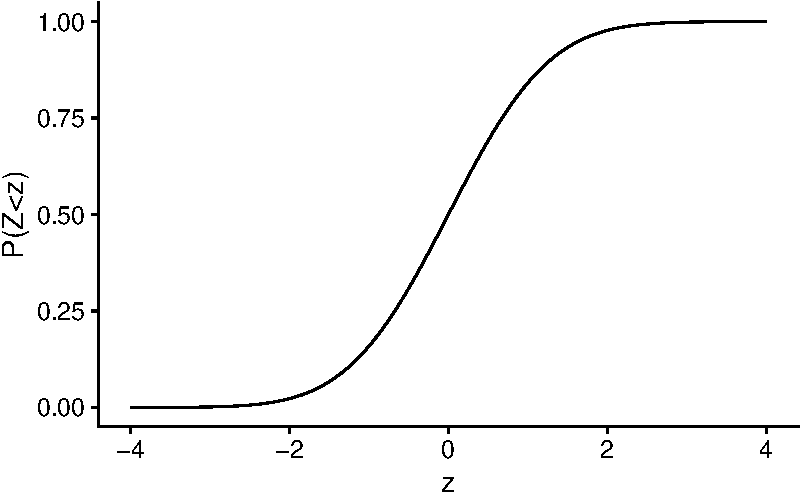
\includegraphics{Reg_files/figure-pdf/fig-snvf-1.pdf}

}

\caption{\label{fig-snvf}Verteilungsfunktion einer
N(0,1)-Zufallsvariable}

\end{figure}%

Da die abhängige Variable eine nichtlineare Funktion der Regressoren
ist, hat der Koeffizient von \(X\) keine einfache Interpretation. Die
Änderung in der Wahrscheinlichkeit, dass \(Y=1\) ist, durch eine
Änderung in \(X\) (partieller Effekt) kann berechnet werden als:

\begin{align}
  \frac{\partial\textup{E}(Y\vert X)}{\partial X} = \frac{\partial\textup{P}(Y=1\vert X)}{\partial X} = \frac{\partial\Phi(\beta_0 + \beta_1 X)}{\partial X} = \phi(\beta_0 + \beta_1 X) \beta_1,
\end{align} wobei \(\phi(\cdot)\) die Dichtefunktion der
Standardnormalverteilung ist. In empirischen Anwendungen wird der
partielle Effekt häufig als Differenz in geschätzten
Wahrscheinlichkeiten angegeben:

\begin{enumerate}
\def\labelenumi{\arabic{enumi}.}
\tightlist
\item
  Berechne die geschätzte Wahrscheinlichkeit, dass \(Y=1\) für einen
  Bezugswert \(X\).
\item
  Berechne die geschätzte Wahrscheinlichkeit, dass \(Y=1\) für
  \(X + \Delta X\).
\item
  Berechne die Differenz zwischen der geschätzten Wahrscheinlichkeiten.
\end{enumerate}

Wie im linearen Wahrscheinlichkeitsmodell kann das Modell
\eqref{eq:probitmodel} auf eine Probit-Regression mit mehreren
Regressoren \(X_j\), \(j=1,\dots,k\) verallgemeinert werden, um das
Risiko einer Verzerrung durch ausgelassene Variablen zu mindern. Die
Schritte 1 bis 3 für die Berechnung des partiellen Effekts einer
Änderung in \(X_j\) erfolgen dann unter der Annahme, dass die übrigen
\(k-1\) Regressoren konstant gehalten werden, wobei der partielle Effekt
von den jeweiligen Regressorwerten abhängt.

\subsection{Logistische Regression}\label{logistische-regression}

\subsection{Schätzung mit R}\label{schuxe4tzung-mit-r}

\begin{Shaded}
\begin{Highlighting}[]
\CommentTok{\# Daten simulieren}
\FunctionTok{set.seed}\NormalTok{(}\DecValTok{1234}\NormalTok{)}

\NormalTok{n }\OtherTok{\textless{}{-}} \DecValTok{2000} \CommentTok{\# Stichprobengröße}

\NormalTok{simdata }\OtherTok{\textless{}{-}} \FunctionTok{tibble}\NormalTok{(}
  \AttributeTok{X =} \FunctionTok{rnorm}\NormalTok{(}\AttributeTok{n =}\NormalTok{ n, }\AttributeTok{mean =} \DecValTok{5}\NormalTok{, }\AttributeTok{sd =} \DecValTok{2}\NormalTok{), }\CommentTok{\# Regressor}
  \AttributeTok{P =} \FunctionTok{pnorm}\NormalTok{(}\FloatTok{0.75} \SpecialCharTok{*}\NormalTok{ X }\SpecialCharTok{{-}} \DecValTok{4} \SpecialCharTok{+} \FunctionTok{rnorm}\NormalTok{(n)), }\CommentTok{\# + Rauschen}
\NormalTok{)}

\CommentTok{\# Binäre Outcome{-}Variable hinzufügen}
\NormalTok{simdata }\OtherTok{\textless{}{-}}\NormalTok{ simdata }\SpecialCharTok{\%\textgreater{}\%}
  \FunctionTok{mutate}\NormalTok{(}\AttributeTok{Y =} \FunctionTok{as.integer}\NormalTok{(}\FunctionTok{runif}\NormalTok{(n) }\SpecialCharTok{\textless{}}\NormalTok{ P))}
\end{Highlighting}
\end{Shaded}

\begin{Shaded}
\begin{Highlighting}[]
\CommentTok{\# lineares Wahrscheinlichkeitsmodell schätzen}
\NormalTok{mod\_lp }\OtherTok{\textless{}{-}} \FunctionTok{lm}\NormalTok{(}\AttributeTok{formula =}\NormalTok{ Y }\SpecialCharTok{\textasciitilde{}}\NormalTok{ X, }\AttributeTok{data =}\NormalTok{ simdata)}
\end{Highlighting}
\end{Shaded}

\begin{Shaded}
\begin{Highlighting}[]
\CommentTok{\# geschätzte Wahrscheinlichkeitsfunktion}
\CommentTok{\# für lineares Modell}
\NormalTok{X }\OtherTok{\textless{}{-}} \FunctionTok{seq}\NormalTok{(}\DecValTok{0}\NormalTok{, }\DecValTok{11}\NormalTok{, }\FloatTok{0.01}\NormalTok{)}

\NormalTok{pred }\OtherTok{\textless{}{-}} \FunctionTok{tibble}\NormalTok{(}
  \AttributeTok{X =}\NormalTok{ X, }
  \AttributeTok{LP =} \FunctionTok{predict}\NormalTok{(}
    \AttributeTok{object =}\NormalTok{ mod\_lp, }
    \AttributeTok{newdata =} \FunctionTok{tibble}\NormalTok{(X)}
\NormalTok{  )}
\NormalTok{)}
\end{Highlighting}
\end{Shaded}

\begin{Shaded}
\begin{Highlighting}[]
\CommentTok{\# geschätztes lineares Modell plotten}
\NormalTok{simdata }\SpecialCharTok{\%\textgreater{}\%}
  \FunctionTok{ggplot}\NormalTok{(}\AttributeTok{mapping =} \FunctionTok{aes}\NormalTok{(}\AttributeTok{x =}\NormalTok{ X, }\AttributeTok{y =}\NormalTok{ Y)) }\SpecialCharTok{+}
  \FunctionTok{geom\_point}\NormalTok{(}
    \AttributeTok{position =} \FunctionTok{position\_jitter}\NormalTok{(}
      \AttributeTok{height =}\NormalTok{ .}\DecValTok{025}\NormalTok{,}
      \AttributeTok{seed =} \DecValTok{1234}
\NormalTok{    ),}
    \AttributeTok{alpha =}\NormalTok{ .}\DecValTok{25}\NormalTok{,}
    \AttributeTok{color =} \StringTok{"blue"}
\NormalTok{  ) }\SpecialCharTok{+}
  \FunctionTok{geom\_line}\NormalTok{(}
    \AttributeTok{data =}\NormalTok{ pred, }
    \AttributeTok{mapping =} \FunctionTok{aes}\NormalTok{(}\AttributeTok{y =}\NormalTok{ LP),}
    \AttributeTok{lwd =}\NormalTok{ .}\DecValTok{75}
\NormalTok{  ) }\SpecialCharTok{+}
  \FunctionTok{theme\_cowplot}\NormalTok{()}
\end{Highlighting}
\end{Shaded}

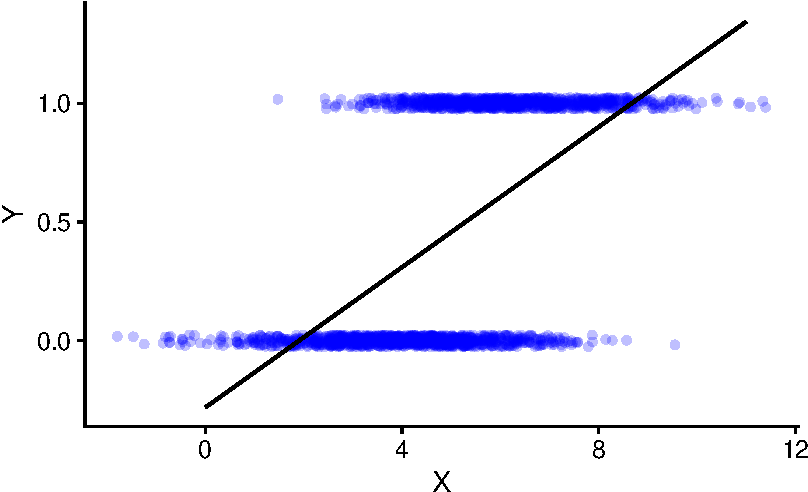
\includegraphics{Reg_files/figure-pdf/unnamed-chunk-6-1.pdf}

\begin{Shaded}
\begin{Highlighting}[]
\CommentTok{\# Probit{-}Modell schätzen}
\NormalTok{mod\_probit }\OtherTok{\textless{}{-}} \FunctionTok{glm}\NormalTok{(}
  \AttributeTok{formula =}\NormalTok{ Y }\SpecialCharTok{\textasciitilde{}}\NormalTok{ X,}
  \AttributeTok{data =}\NormalTok{ simdata, }
  \AttributeTok{family =} \FunctionTok{binomial}\NormalTok{(}\AttributeTok{link =} \StringTok{"probit"}\NormalTok{)}
\NormalTok{)}
\end{Highlighting}
\end{Shaded}

\begin{Shaded}
\begin{Highlighting}[]
\CommentTok{\# Logit{-}Modell schätzen}
\NormalTok{mod\_logit }\OtherTok{\textless{}{-}} \FunctionTok{glm}\NormalTok{(}
  \AttributeTok{formula =}\NormalTok{ Y }\SpecialCharTok{\textasciitilde{}}\NormalTok{ X,}
  \AttributeTok{data =}\NormalTok{ simdata, }
  \AttributeTok{family =} \FunctionTok{binomial}\NormalTok{(}\AttributeTok{link =} \StringTok{"logit"}\NormalTok{)}
\NormalTok{)}
\end{Highlighting}
\end{Shaded}

\begin{Shaded}
\begin{Highlighting}[]
\CommentTok{\# gesch. WSK{-}Funktion für Probit{-} und Logit{-}Modelle}
\NormalTok{pred }\OtherTok{\textless{}{-}}\NormalTok{ pred }\SpecialCharTok{\%\textgreater{}\%}
  \FunctionTok{mutate}\NormalTok{(}
    \AttributeTok{Probit =} \FunctionTok{predict}\NormalTok{(mod\_probit, }\FunctionTok{tibble}\NormalTok{(X), }\AttributeTok{type =} \StringTok{"response"}\NormalTok{),}
    \AttributeTok{Logit =} \FunctionTok{predict}\NormalTok{(mod\_logit, }\FunctionTok{tibble}\NormalTok{(X), }\AttributeTok{type =} \StringTok{"response"}\NormalTok{)}
\NormalTok{  ) }\SpecialCharTok{\%\textgreater{}\%}
  \FunctionTok{pivot\_longer}\NormalTok{(}
  \AttributeTok{cols =}\NormalTok{ LP}\SpecialCharTok{:}\NormalTok{Logit, }
  \AttributeTok{names\_to =} \StringTok{"Methode"}\NormalTok{, }
  \AttributeTok{values\_to =} \StringTok{"Wsk"}
\NormalTok{)}
\end{Highlighting}
\end{Shaded}

\begin{Shaded}
\begin{Highlighting}[]
\CommentTok{\# Vergleich mit linearem Modell}
\NormalTok{simdata }\SpecialCharTok{\%\textgreater{}\%}
  \FunctionTok{ggplot}\NormalTok{(}\AttributeTok{mapping =} \FunctionTok{aes}\NormalTok{(}\AttributeTok{x =}\NormalTok{ X, }\AttributeTok{y =}\NormalTok{ Y) ) }\SpecialCharTok{+}
  \FunctionTok{geom\_point}\NormalTok{(}
    \AttributeTok{position =} \FunctionTok{position\_jitter}\NormalTok{(}
      \AttributeTok{height =}\NormalTok{ .}\DecValTok{01}\NormalTok{, }
      \AttributeTok{seed =} \DecValTok{1234}
\NormalTok{    )}
\NormalTok{  ) }\SpecialCharTok{+}
  \FunctionTok{geom\_line}\NormalTok{(}
    \AttributeTok{data =}\NormalTok{ pred, }
    \AttributeTok{mapping =} \FunctionTok{aes}\NormalTok{(}\AttributeTok{y =}\NormalTok{ Wsk, }\AttributeTok{color =}\NormalTok{ Methode)}
\NormalTok{  ) }\SpecialCharTok{+}
  \FunctionTok{scale\_y\_continuous}\NormalTok{(}\AttributeTok{breaks =} \FunctionTok{c}\NormalTok{(}\DecValTok{0}\NormalTok{, }\DecValTok{1}\NormalTok{)) }\SpecialCharTok{+}
  \FunctionTok{theme\_cowplot}\NormalTok{()}
\end{Highlighting}
\end{Shaded}

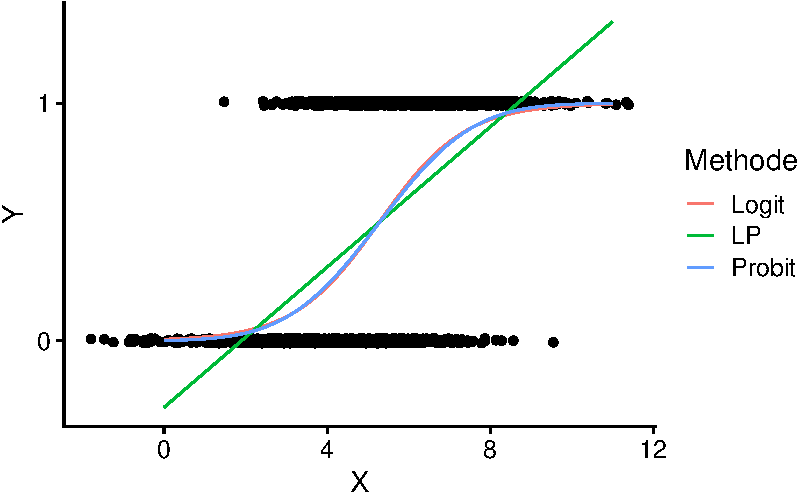
\includegraphics{Reg_files/figure-pdf/unnamed-chunk-10-1.pdf}

\section{Modellierung von Zählvariablen mit
Poisson-Regression}\label{sec-poissonreg}

Die Poisson-Regression ist ein statistisches Modell, das verwendet wird,
um Zählvariablen (d.h. Variablen, die diskrete, nicht-negative Werte
annehmen) zu modellieren, insbesondere wenn die Zählwerte eine
Poisson-Verteilung aufweisen. Dieses Modell wird häufig in Fällen
verwendet, in denen die abhängige Variable die Anzahl der Ereignisse in
einem bestimmten Zeitraum oder Raum beschreibt, wie z.B. die Anzahl der
Verkehrsunfälle in einer Stadt innerhalb eines Monats.

\subsection{Poisson-Verteilung}\label{poisson-verteilung}

Eine Zufallsvariable \(Y\) folgt einer Poisson-Verteilung mit Parameter
\(\lambda\), wenn ihre Wahrscheinlichkeitsverteilung gegeben ist durch:

\begin{align}
P(Y = y) = \frac{\lambda^y e^{-\lambda}}{y!} \quad \text{für} \quad y = 0, 1, 2, \ldots
\end{align}

Hierbei ist \(\lambda\) sowohl der Mittelwert als auch die Varianz der
Verteilung (\(\mathbb{E}[Y] = \text{Var}(Y) = \lambda\)).

\begin{Shaded}
\begin{Highlighting}[]
\NormalTok{n }\OtherTok{\textless{}{-}} \DecValTok{500}
\NormalTok{dat }\OtherTok{\textless{}{-}} \FunctionTok{tibble}\NormalTok{(}
  \AttributeTok{Y =} \FunctionTok{rpois}\NormalTok{(}\AttributeTok{n =}\NormalTok{ n, }\AttributeTok{lambda =} \DecValTok{5}\NormalTok{)}
\NormalTok{)}
\end{Highlighting}
\end{Shaded}

\begin{Shaded}
\begin{Highlighting}[]
\FunctionTok{ggplot}\NormalTok{(}
    \AttributeTok{data =}\NormalTok{ dat, }
    \AttributeTok{mapping =} \FunctionTok{aes}\NormalTok{(}\AttributeTok{x =}\NormalTok{ Y)}
\NormalTok{) }\SpecialCharTok{+}
    \FunctionTok{geom\_histogram}\NormalTok{(}
        \AttributeTok{mapping =} \FunctionTok{aes}\NormalTok{(}\AttributeTok{y =} \FunctionTok{after\_stat}\NormalTok{(density)), }
        \AttributeTok{binwidth =} \DecValTok{1}\NormalTok{, }
        \AttributeTok{color =} \StringTok{"white"}
\NormalTok{    ) }\SpecialCharTok{+}
    \FunctionTok{geom\_line}\NormalTok{(}
        \AttributeTok{data =} \FunctionTok{tibble}\NormalTok{(}
            \AttributeTok{X =} \DecValTok{0}\SpecialCharTok{:}\DecValTok{13}\NormalTok{,}
            \AttributeTok{Y =} \FunctionTok{dpois}\NormalTok{(}\AttributeTok{x =}\NormalTok{ X, }\AttributeTok{lambda =} \DecValTok{5}\NormalTok{)}
\NormalTok{        ),}
        \AttributeTok{mapping =} \FunctionTok{aes}\NormalTok{(}\AttributeTok{x =}\NormalTok{ X, }\AttributeTok{y =}\NormalTok{ Y),}
        \AttributeTok{color =} \StringTok{"red"}
\NormalTok{    ) }\SpecialCharTok{+}
    \FunctionTok{theme\_cowplot}\NormalTok{()}
\end{Highlighting}
\end{Shaded}

\begin{figure}[t]

\centering{

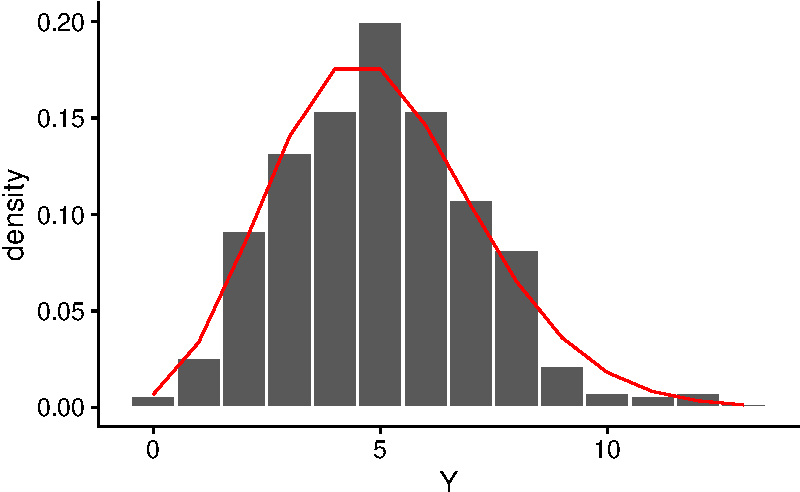
\includegraphics{Reg_files/figure-pdf/fig-poissonexample-1.pdf}

}

\caption{\label{fig-poissonexample}Stichprobenverteilung und
Poisson-Dichtefunktion}

\end{figure}%

\subsection{Der Regressionsansatz}\label{der-regressionsansatz}

In der Poisson-Regression modellieren wir den Erwartungswert der
abhängigen Variable \(Y\) als eine Funktion der unabhängigen Variablen
\(\mathbf{X} = (X_1, X_2, \ldots, X_k)\). Der Erwartungswert von \(Y\)
wird durch den Parameter \(\lambda\) repräsentiert, der wiederum eine
Funktion der unabhängigen Variablen ist. Die Beziehung wird
typischerweise durch eine logarithmische Verknüpfungsfunktion
beschrieben:

\begin{align}
\log(\lambda_i) = \mathbf{X}_i^\top \boldsymbol{\beta}
\end{align}

Dies kann auch als

\begin{align}
\lambda_i = \exp(\mathbf{X}_i^\top \boldsymbol{\beta})
\end{align}

geschrieben werden, wobei:

\begin{itemize}
\item
  \(\lambda_i\) der Erwartungswert von \(Y\) für Beobachtung \(i\),
\item
  \(\mathbf{X}_i\) der Vektor der unabhängigen Variablen für Beobachtung
  \(i\) und
\item
  \(\boldsymbol{\beta}\) der Vektor der Regressionskoeffizienten ist.
\end{itemize}

\subsection{Modellanpassung}\label{modellanpassung}

Die Parameter \(\boldsymbol{\beta}\) werden durch
Maximum-Likelihood-Schätzung (MLE) geschätzt. Die Likelihood-Funktion
für \(n\) Beobachtungen ist gegeben durch

\begin{align}
L(\boldsymbol{\beta}) = \prod_{i=1}^n \frac{\lambda_i^{y_i} e^{-\lambda_i}}{y_i!}.
\end{align}

Die Log-Likelihood-Funktion ist daher

\begin{align}
\mathcal{L}(\boldsymbol{\beta}) = \sum_{i=1}^n \left( y_i \log(\lambda_i) - \lambda_i - \log(y_i!). \right)
\end{align}

Da \(\lambda_i = \exp(\mathbf{X}_i^\top \boldsymbol{\beta})\), wird die
Log-Likelihood-Funktion zu

\begin{align}
\mathcal{L}(\boldsymbol{\beta}) = \sum_{i=1}^n \left( y_i (\mathbf{X}_i^\top \boldsymbol{\beta}) - \exp(\mathbf{X}_i^\top \boldsymbol{\beta}) - \log(y_i!) \right)
\end{align}

Den Maximum-Likelihood-Schätzer \(\widehat{\boldsymbol{\beta}}\)
erhalten wir durch Maximierung der Log-Likelihoodfunktion
\(\mathcal{L}(\boldsymbol{\beta})\). Eine R-Implementierung finden wir
in \texttt{stats::glm()}.

\subsection{Interpretation der
Koeffizienten}\label{interpretation-der-koeffizienten}

Die Koeffizienten \(\boldsymbol{\beta}\) in der Poisson-Regression haben
eine log-lineare Beziehung zur Zählvariable. Für einen bestimmten
Koeffizienten \(\beta_j\) ist die Interpretation wiefolgt:

\begin{itemize}
\item
  Ein Anstieg der unabhängigen Variable \(X_j\) um eine Einheit führt zu
  einer Änderung des \emph{Logarithmus} des Erwartungswertes von \(Y\)
  um \(\beta_j\).
\item
  Der Erwartungswert \(\lambda\) ändert sich \emph{multiplikativ} um
  \(\exp(\beta_j)\).
\end{itemize}

Angenommen, wir haben eine unabhängige Variable \(X\) (z.B. die Anzahl
der durchgeführten Werbekampagnen) und eine Zählvariable \(Y\) (z.B. die
Anzahl der Verkäufe). Das Modell könnte wie folgt aussehen:

\begin{align}
\log(\lambda) = \beta_0 + \beta_1 X
\end{align}

Wenn \(\beta_1 = 0.5\), bedeutet dies, dass jede zusätzliche
Werbekampagne die erwartete Anzahl der Verkäufe um einen Faktor von
\(\exp(0.5) \approx 1.65\) erhöht. Das heißt, die \emph{Rate} der
Verkäufe steigt um 65\% für jede zusätzliche Werbekampagne.

\begin{Shaded}
\begin{Highlighting}[]
\CommentTok{\# Setze den Zufallszahlengenerator für Reproduzierbarkeit}
\CommentTok{\#set.seed(1234)}

\CommentTok{\# Anzahl der Beobachtungen}
\NormalTok{n }\OtherTok{\textless{}{-}} \DecValTok{500}

\CommentTok{\# Simuliere die unabhängige Variable X (Anzahl der Werbekampagnen)}
\NormalTok{X }\OtherTok{\textless{}{-}} \FunctionTok{sample}\NormalTok{(}\DecValTok{1}\SpecialCharTok{:}\DecValTok{8}\NormalTok{, }\AttributeTok{replace =}\NormalTok{ T, }\AttributeTok{size =}\NormalTok{ n)}

\CommentTok{\# Setze die wahren Parameter für das Modell}
\NormalTok{beta\_1 }\OtherTok{\textless{}{-}} \FloatTok{0.4}  \CommentTok{\# Koeffizient für X}

\CommentTok{\# Berechne den Erwartungswert lambda basierend auf dem Modell}
\NormalTok{lambda }\OtherTok{\textless{}{-}} \FunctionTok{exp}\NormalTok{(}\DecValTok{2} \SpecialCharTok{+}\NormalTok{ beta\_1 }\SpecialCharTok{*}\NormalTok{ X)}

\CommentTok{\# Simuliere die abhängige Variable Y (Anzahl der Verkäufe) als Poisson{-}verteilte Zufallsvariable}
\NormalTok{Y }\OtherTok{\textless{}{-}} \FunctionTok{rpois}\NormalTok{(n, }\AttributeTok{lambda =}\NormalTok{ lambda)}

\NormalTok{dat }\OtherTok{\textless{}{-}} \FunctionTok{tibble}\NormalTok{(}\AttributeTok{X =}\NormalTok{ X, }\AttributeTok{Y =}\NormalTok{ Y)}
\end{Highlighting}
\end{Shaded}

\begin{Shaded}
\begin{Highlighting}[]
\FunctionTok{ggplot}\NormalTok{(}
  \AttributeTok{data =}\NormalTok{ dat, }
  \AttributeTok{mapping =} \FunctionTok{aes}\NormalTok{(}\AttributeTok{x =}\NormalTok{ Y)}
\NormalTok{  ) }\SpecialCharTok{+}
  \FunctionTok{geom\_histogram}\NormalTok{(}\AttributeTok{binwidth =} \DecValTok{2}\NormalTok{) }\SpecialCharTok{+}
  \FunctionTok{theme\_cowplot}\NormalTok{()}
\end{Highlighting}
\end{Shaded}

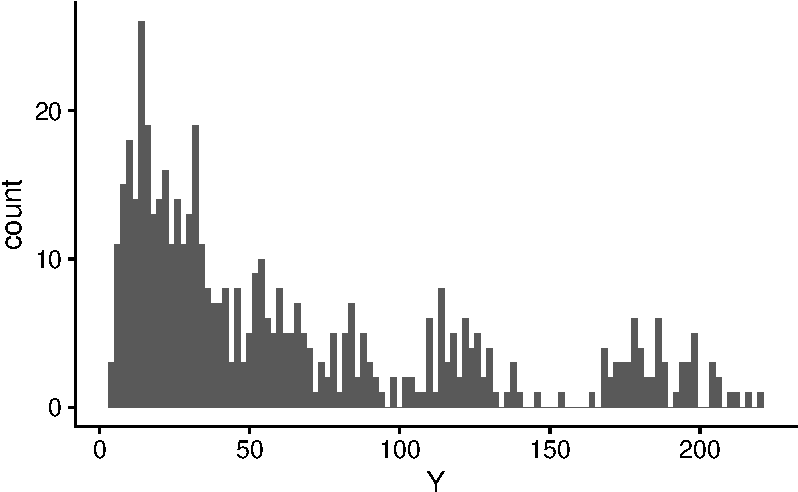
\includegraphics{Reg_files/figure-pdf/unnamed-chunk-14-1.pdf}

\begin{Shaded}
\begin{Highlighting}[]
\CommentTok{\# Poisson{-}Regression schätzen}
\NormalTok{model }\OtherTok{\textless{}{-}} \FunctionTok{glm}\NormalTok{(}
  \AttributeTok{formula =}\NormalTok{ Y }\SpecialCharTok{\textasciitilde{}}\NormalTok{ X, }
  \AttributeTok{family =} \FunctionTok{poisson}\NormalTok{(}\AttributeTok{link =} \StringTok{"log"}\NormalTok{), }
  \AttributeTok{data =}\NormalTok{ dat}
\NormalTok{)}

\CommentTok{\# Zusammenfassung des gesch. Modells}
\FunctionTok{summary}\NormalTok{(model)}
\end{Highlighting}
\end{Shaded}

\begin{verbatim}

Call:
glm(formula = Y ~ X, family = poisson(link = "log"), data = dat)

Coefficients:
            Estimate Std. Error z value Pr(>|z|)    
(Intercept) 1.996150   0.019432   102.7   <2e-16 ***
X           0.402650   0.002977   135.3   <2e-16 ***
---
Signif. codes:  0 '***' 0.001 '**' 0.01 '*' 0.05 '.' 0.1 ' ' 1

(Dispersion parameter for poisson family taken to be 1)

    Null deviance: 22952.0  on 499  degrees of freedom
Residual deviance:   527.4  on 498  degrees of freedom
AIC: 3329.2

Number of Fisher Scoring iterations: 4
\end{verbatim}

\begin{Shaded}
\begin{Highlighting}[]
\CommentTok{\# Vorhersagen}
\NormalTok{dat}\SpecialCharTok{$}\NormalTok{predicted }\OtherTok{\textless{}{-}} \FunctionTok{predict}\NormalTok{(model, }\AttributeTok{type =} \StringTok{"response"}\NormalTok{)}

\CommentTok{\# Simulierte Daten und Schätzungen}
\FunctionTok{ggplot}\NormalTok{(}
  \AttributeTok{data =}\NormalTok{ dat, }
  \AttributeTok{mapping =} \FunctionTok{aes}\NormalTok{(}\AttributeTok{x =}\NormalTok{ X, }\AttributeTok{y =}\NormalTok{ Y)}
\NormalTok{) }\SpecialCharTok{+}
  \FunctionTok{geom\_point}\NormalTok{(}
    \AttributeTok{mapping =} \FunctionTok{aes}\NormalTok{(}\AttributeTok{color =} \StringTok{"Simulierte Daten"}\NormalTok{), }
    \AttributeTok{alpha =} \FloatTok{0.5}\NormalTok{, }
    \AttributeTok{position =} \FunctionTok{position\_jitter}\NormalTok{(}\AttributeTok{width =}\NormalTok{ .}\DecValTok{1}\NormalTok{)}
\NormalTok{  ) }\SpecialCharTok{+}
  \FunctionTok{geom\_line}\NormalTok{(}
    \FunctionTok{aes}\NormalTok{(}\AttributeTok{y =}\NormalTok{ predicted, }\AttributeTok{color =} \StringTok{"Geschätztes Modell"}\NormalTok{)}
\NormalTok{    ) }\SpecialCharTok{+}
  \FunctionTok{labs}\NormalTok{(}
    \AttributeTok{x =} \StringTok{"Anzahl der Werbekampagnen"}\NormalTok{,}
    \AttributeTok{y =} \StringTok{"Anzahl der Eisverkäufe"}
\NormalTok{  ) }\SpecialCharTok{+}
  \FunctionTok{scale\_color\_manual}\NormalTok{(}
    \StringTok{""}\NormalTok{,}
    \AttributeTok{values =} \FunctionTok{c}\NormalTok{(}
      \StringTok{"Simulierte Daten"} \OtherTok{=} \StringTok{"blue"}\NormalTok{, }
      \StringTok{"Geschätztes Modell"} \OtherTok{=} \StringTok{"red"}
\NormalTok{    )}
\NormalTok{  ) }\SpecialCharTok{+}
  \FunctionTok{theme\_cowplot}\NormalTok{() }\SpecialCharTok{+}
  \FunctionTok{theme}\NormalTok{(}\AttributeTok{legend.position =} \StringTok{"top"}\NormalTok{)}
\end{Highlighting}
\end{Shaded}

\begin{figure}[t]

\centering{

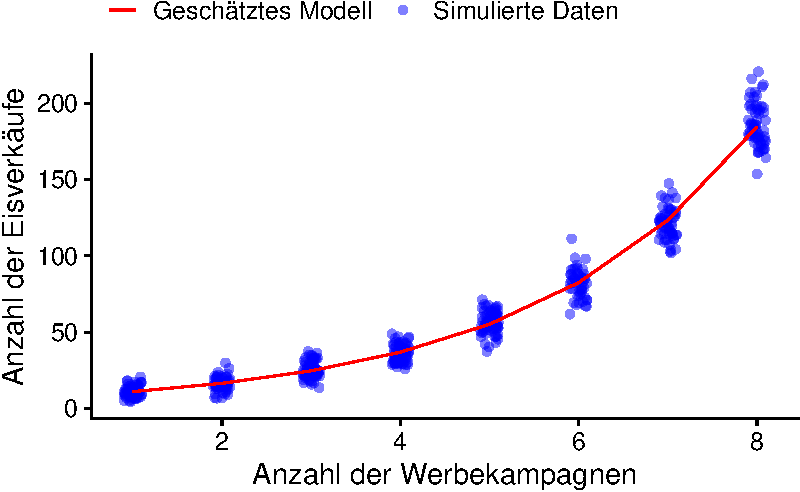
\includegraphics{Reg_files/figure-pdf/fig-poissonregexample-1.pdf}

}

\caption{\label{fig-poissonregexample}Simulierte Daten und angepasstes
Poisson-Modell}

\end{figure}%

\bookmarksetup{startatroot}

\chapter{Matching}\label{matching}

\begin{Shaded}
\begin{Highlighting}[]
\NormalTok{\#| context: setup}
\NormalTok{\# create dataset directory}
\NormalTok{dir.create("datasets")}
\NormalTok{\# Download the dataset}
\NormalTok{download.file(}
\NormalTok{    "https://raw.githubusercontent.com/mca91/kausal\_data/main/darkmode.csv",}
\NormalTok{    \textquotesingle{}datasets/darkmode.csv\textquotesingle{},}
\NormalTok{)}
\end{Highlighting}
\end{Shaded}

\begin{Shaded}
\begin{Highlighting}[]
\NormalTok{\#| context: setup}
\NormalTok{library(dplyr)}
\NormalTok{\# make darkmode available using read.csv for now}
\NormalTok{\# because there\textquotesingle{}s some issue with readr::read\_csv}
\NormalTok{\# I can\textquotesingle{}t fix right now}
\NormalTok{darkmode \textless{}{-} read.csv(}
\NormalTok{    file = "datasets/darkmode.csv", }
\NormalTok{    colClasses = c("numeric", "logical", "numeric", "numeric", "numeric") }
\NormalTok{)}

\NormalTok{options(pillar.bold = TRUE, pillar.subtle = FALSE)}
\end{Highlighting}
\end{Shaded}

In randomisierten kontrollierten Studien stellt eine randomisierte
Behandlung sicher, dass die Individuen beider Gruppen im Mittel
vergleichbar sind, dass heißt es gibt keine systematischen Unterschiede
der Studiensubjekte hinsichtlich der Verteilung von Charakteristika
zwischen den Gruppen. Dann ist es plausibel eine beobachtete mittlere
Differenz in der Outcome-Variable alleine auf die Behandlung
zurückzuführen.

In der Praxis, insbesondere in ökonomischen Studien, sind randomisierte
kontrollierte Studien aus ethischen und/oder finanziellen Gründen nicht
durchführbar. Stattdessen werden nicht-experimentelle Daten genutzt, die
jedoch nur sehr selten eine Vergleichbarkeit von Behandlungs- und
Kontrollgruppe gewährleisten.

In diesem Kapitel betrachten wir Methoden, die in solchen
Forschungsdesigns -- bei hinreichenden Informationen über die
Studiensubjekte -- eine Schätzung kausaler Effekte ermöglichen, indem
eine statistische Vergleichbarkeit von Behandlungs- und Kontrollgruppe
hergestellt wird. Dies kann durch eine gezielte Gewichtung von
Beobachtungen anhand invididueller Merkmale bei der Schätzung des
Behandlungseffekts erfolgen. Andere etablierte Methoden schätzen den
kausalen Effekt nach Selektion von vergleichbaren Teilmengen von
Subjekten beider Gruppen aus der ursprünglichen Stichprobe, sogenanntes
\emph{selektierendes Matching}.

Da Matching Beobachtungen basierend auf beobachtbaren Merkmalen
vergleicht, kann die Wahrscheinlichkeit einer verzerrten Schätzung des
kausalen Effekt durch falsche Modellspezifikationen geringer sein als
für eine Schätzung des Effekts anhand multipler Regression. Weiterhin
basieren Matching-Methoden nicht auf der Annahme eines linearen
Zusammenhangs zwischen Kovariablen und der erklärenden Variable und
können für die Schätzung unterschiedlicher Spezifikationen von
Behandlungseffekten herangezogen werden.

Für die Gültigkeit eines Schätzers basierend auf Matching sind zwei
Annahmen erforderlich.

\begin{enumerate}
\def\labelenumi{\arabic{enumi}.}
\item
  \textbf{\emph{Bedingte Unabhängigkeit.}} Seien \(Y^{(0)}_i\) und
  \(Y^{(1)}_i\) potentielle Ergebnisse der Outcome-Variable \(Y\) für
  ein Subjekt \(i\) mit \(B_i=0\) (keine Zuweisung zur Behandlung)
  beziehungsweise \(B_i=1\) (Behandlung) und \(X_i\) die beobachteten
  Kovariablen. Wir nehmen an, dass \begin{align}
    \left\{Y^{(0)}_i, Y^{(1)}_i\right\} \perp B_i\vert X_i, \label{eq:cia}
  \end{align} d.h. die Behandlungszuweisung/-selektion ist unanabhängig
  von den potentielle Ergebnissen \(Y^{(0)}_i\) und \(Y^{(1)}_i\), wenn
  wir für die Kovariablen \(X\) kontrollieren.
\item
  \textbf{\emph{Überlappung.}} Für jede mögliche Kombination von
  Kovariablen \(X_i\) gibt es eine positive Wahrscheinlichkeit \(<1\),
  sowohl zur Behandlungsgruppe (\(B_i = 1\)) als auch zur Kontrollgruppe
  (\(B_i = 0\)) zugewiesen zu werden, \begin{align}
    0 < \text{P}(B_i=1\lvert X_i) < 1, \label{eq:overlap}
  \end{align} d.h. keine Beobachtung hat eine
  Behandlungswahrscheinlichkeit von exakt \(0\) oder \(1\).
\end{enumerate}

Annahme 1 stellt sicher, dass die Zuweisung zur Behandlungsgruppe nach
Kontrolle für die Kovariablen \(X\) als zufällig betracht werden kann.
Somit ist es möglich den kausalen Effekt der Behandlung zu
identifizieren, indem wir hinsichtlich der Kovariablen \(X\) ähnliche
Subjekte (vgl. Annahme 2) aus Kontroll- und Behandlungsgruppe
vergleichen.

Annahme 2 setzt vorraus, dass es eine ausreichende Überlappung in den
Verteilungen der Kovariablen zwischen Behandlungs- und Kontrollgruppe
gibt. Dann ist sichergestellt, dass für jedes Subjekt in einer Gruppe
ein hinsichtlich seiner Charakteristika vergleichbares Subjekt in der
anderen Gruppe geben kann, sodass ein Vergleich möglich ist.

\section{\texorpdfstring{\emph{Balance}: Vergleichbarkeit von
Behandlungs- und
Kontrollgruppe}{Balance: Vergleichbarkeit von Behandlungs- und Kontrollgruppe}}\label{sec-balance}

Der Lehrstuhl für Ökonometrie an der Universität Duisburg-Essen betreibt
einen Ökonometrie-Blog und interessiert sich für den kausalen Effekt der
Einführung eines
\href{https://en.wikipedia.org/wiki/Wikipedia:Dark_mode}{darkmode} auf
die Verweildauer der User auf der Webseite. Die Webseite ist zwar
nicht-kommerziell, hat sich allerdings insb. für die Aquise
internationaler Studierender für den Studiengang MSc. Econometrics als
wichtiges Marketing-Instrument erwiesen. Ein anprechendes Design wird
daher als hoch-relevant erachtet.

Idealerweise sollte der Effekt des Design-Relaunches auf die
Nutzungsintensität in einem kontrollierten randomisierten Experiment
untersucht werden. Hierbei würden wir Nutzern zufällig das neue oder das
alte Design zuweisen und den Effekt als Differnz des durchschnittlichen
Verweildauer für die Gruppen bestimmen. Eine solche Studie ist jedoch
aus technischen und finanziellen Gründen nicht realisierbar, sodass die
Auswirkungen des darkmode mit vorliegenden nicht-experimenellen
Nutzungsstatistiken für die Webseite geschätzt werden sollen.

Die Nutzungsstatistiken sind im Datensatz
\href{https://raw.githubusercontent.com/mca91/kasa_data/main/darkmode.csv}{\emph{darkmode.csv}}
enthalten und sollen der Analyse des Effekts des darkmode
(\texttt{dark\_mode}) auf die Verweildauer der Leser auf der Webseite
(\texttt{read\_time}) dienen.

Tabelle~\ref{tbl-darkmode} zeigt die Definitionen der Variablen in
\emph{darkmode.csv}.

\begin{longtable}{ll}

\caption{\label{tbl-darkmode}Variablen im Datensatz \emph{darkmode}}

\tabularnewline

\toprule
Variable & Beschreibung \\ 
\midrule\addlinespace[2.5pt]
read\_time & Lesezeit (Minuten/Woche) \\ 
dark\_mode & Indikator: Beobachtung nach Einführung darkmode \\ 
male & Indikator: Individuum männlich \\ 
age & Alter (in Jahren) \\ 
hours & Bisherige Verweildauer auf der Seite \\ 
\bottomrule

\end{longtable}

Für die Analyse lesen wir zunächst den Datensatz \emph{darkmode.csv} mit
\texttt{readr::read\_csv()} ein und verschaffen uns einen Überblick über
die verfügbaren Variablen.

\begin{Shaded}
\begin{Highlighting}[]
\CommentTok{\# Paket \textasciigrave{}tidyverse\textasciigrave{} laden}
\FunctionTok{library}\NormalTok{(tidyverse)}

\CommentTok{\# Datensatz \textquotesingle{}darkmode\textquotesingle{} einlesen}
\NormalTok{darkmode }\OtherTok{\textless{}{-}} \FunctionTok{read\_csv}\NormalTok{(}
  \AttributeTok{file =} \StringTok{"datasets/darkmode.csv"}
\NormalTok{)}
\end{Highlighting}
\end{Shaded}

\texttt{dark\_mode} hat den Typ \texttt{logical}. Mit
\texttt{dplyr::mutate\_all()} können wir komfortabel alle Spalten in den
Typ \texttt{numeric} transformieren.

\begin{Shaded}
\begin{Highlighting}[]
\CommentTok{\# Alle Variablen zu typ \textquotesingle{}numeric\textquotesingle{} formatieren...}
\NormalTok{darkmode }\OtherTok{\textless{}{-}}\NormalTok{ darkmode }\SpecialCharTok{\%\textgreater{}\%} 
  \FunctionTok{mutate\_all}\NormalTok{(}\AttributeTok{.funs =}\NormalTok{ as.numeric)}

\CommentTok{\# ... und überprüfen}
\FunctionTok{glimpse}\NormalTok{(darkmode)}
\end{Highlighting}
\end{Shaded}

\begin{verbatim}
Rows: 300
Columns: 5
$ read_time <dbl> 14.4, 15.4, 20.9, 20.0, 21.5, 19.5, 22.0, 17.4, 23.6, 15.7, ~
$ dark_mode <dbl> 0, 0, 1, 0, 1, 0, 1, 0, 0, 0, 0, 1, 0, 1, 1, 1, 1, 0, 0, 0, ~
$ male      <dbl> 0, 1, 0, 0, 0, 0, 0, 0, 0, 0, 0, 1, 0, 1, 0, 1, 0, 1, 0, 0, ~
$ age       <dbl> 43, 55, 23, 41, 29, 64, 18, 53, 59, 53, 43, 38, 42, 23, 39, ~
$ hours     <dbl> 65.6, 125.4, 642.6, 129.1, 190.2, 185.3, 333.5, 279.3, 1302.~
\end{verbatim}

Eine naive Schätzung des durchschnittlichen Behandlungseffekts (ATE)
\(\widehat{\tau}^{\text{naiv}}\) erhalten wir als Mittelwertdifferenz
von \texttt{read\_time} für die Behandlungsgruppe
(\texttt{dark\_mode\ ==\ 1}) und die Kontrollgruppe
(\texttt{dark\_mode\ ==\ 0}) \begin{align}
  \widehat{\tau}^{\text{naiv}} = \overline{\text{read\_time}}_{\text{Behandlung}} - \overline{\text{read\_time}}_{\text{Kontrolle}}.\label{eq:naivATEdarkmode}
\end{align}

Diese Berechnung ist schnell mit R durchgeführt.

\begin{Shaded}
\begin{Highlighting}[]
\CommentTok{\# Naiver Schätzer für ATE: }
\CommentTok{\# Differenz der Gruppen{-}Durchschnitte}

\CommentTok{\# Outcome in Behandlungsgruppe}
\NormalTok{read\_time\_mTG }\OtherTok{\textless{}{-}}\NormalTok{ darkmode }\SpecialCharTok{\%\textgreater{}\%} 
  \FunctionTok{filter}\NormalTok{(dark\_mode }\SpecialCharTok{==} \DecValTok{1}\NormalTok{) }\SpecialCharTok{\%\textgreater{}\%} 
  \FunctionTok{pull}\NormalTok{(}\StringTok{"read\_time"}\NormalTok{)}

\CommentTok{\# Outcome in Kontrollgruppe}
\NormalTok{read\_time\_mKG }\OtherTok{\textless{}{-}}\NormalTok{ darkmode }\SpecialCharTok{\%\textgreater{}\%} 
  \FunctionTok{filter}\NormalTok{(dark\_mode }\SpecialCharTok{==} \DecValTok{0}\NormalTok{) }\SpecialCharTok{\%\textgreater{}\%} 
  \FunctionTok{pull}\NormalTok{(}\StringTok{"read\_time"}\NormalTok{)}

\CommentTok{\# Mittelwert{-}Differenz}
\FunctionTok{mean}\NormalTok{(read\_time\_mTG) }\SpecialCharTok{{-}} \FunctionTok{mean}\NormalTok{(read\_time\_mKG)}
\end{Highlighting}
\end{Shaded}

\begin{verbatim}
[1] -0.4446331
\end{verbatim}

Die Schätzung ergibt einen negativen Behandlungseffekt, mit der
Interpreation, dass das neue Design zu einer Reduktion der Lesezeit um
etwa 0.44 Minuten pro Woche führt. Dieses Ergebnis ist allerdings
zweifelhaft, weil eine Isolierung des Behandlungseffekts aufgrund von
Backdoor-Pfaden im DGP vermutlich nicht gewähleistet ist. Ein Indikator
hierfür sind systematische Unterschiede hinsichtlich von (möglicherweise
unbeobachtbaren) Charakteristika von Kontrollgruppe und
Behandlungsgruppe.

Da die User sich beim Aufrufen der Seite aktiv für oder gegen den das
neue Design entscheiden müssen (und somit selektieren, ob Sie in der
Behandlungs- oder Kontrollgruppe landen), liegt wahrscheinlich
\emph{Confounding} vor: Unsere Hypothese ist zunächst, dass männliche
User eine durchschnittlich längere Lesezeit aufweisen \emph{und} mit
größerer Wahrscheinlichkeit auf das neue Design wechseln als
nicht-männliche Leser. Dann ist \texttt{male} eine Backdoor-Variable.
Diese Situation ist unter der Annahme, dass nur diese Faktoren den DGP
bestimmen, in Abbildung~\ref{fig-maleCDdarkmode} dargestellt.

\begin{figure}[t]

\centering{

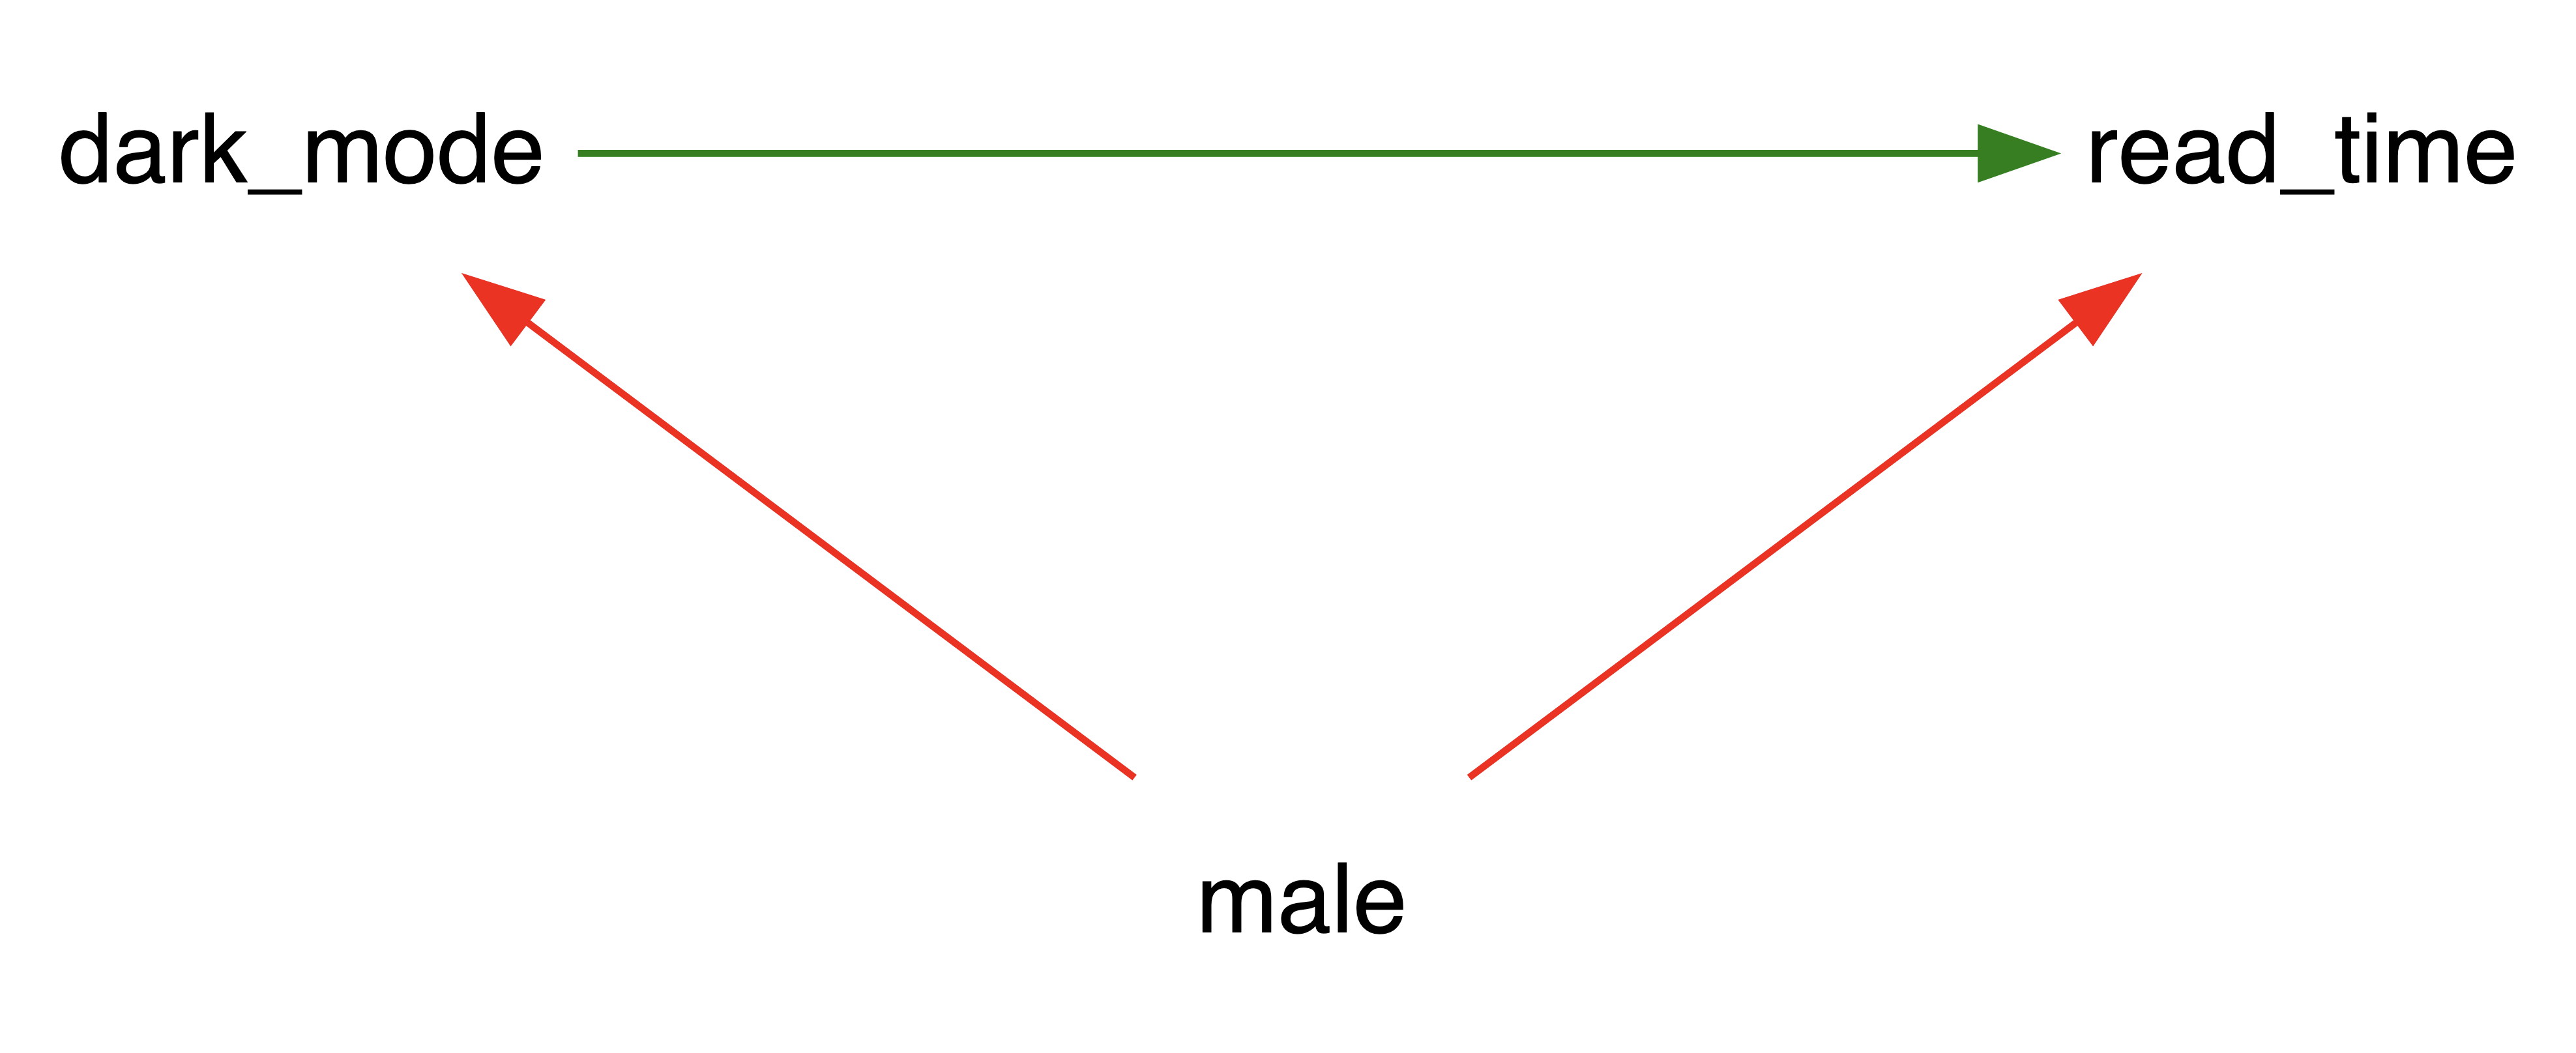
\includegraphics[width=4in,height=3in]{Matching_files/figure-latex/dot-figure-1.png}

}

\caption{\label{fig-maleCDdarkmode}Backdoor durch `male' im
Website-Design-Bespiel}

\end{figure}%

Der DGP in Abbildung~\ref{fig-maleCDdarkmode} führt zu einer verzerrten
Schätzung des kausalen Effekts von \texttt{dark\_mode} auf
\texttt{read\_time} mit \eqref{eq:naivATEdarkmode}, wenn das Verhältnis
von männlichen und nicht-männlichen Usern in Bahandlungs- und
Kontrollgruppe nicht ausgeglichen ist. Wir überprüfen dies mit R.

\begin{Shaded}
\begin{Highlighting}[]
\CommentTok{\# Anteile männlicher und nicht{-}männlicher User}
\NormalTok{(}
\NormalTok{  anteile }\OtherTok{\textless{}{-}}\NormalTok{ darkmode }\SpecialCharTok{\%\textgreater{}\%} 
  \FunctionTok{group\_by}\NormalTok{(dark\_mode) }\SpecialCharTok{\%\textgreater{}\%} 
  \FunctionTok{summarise}\NormalTok{(}
    \AttributeTok{gesamt =} \FunctionTok{n}\NormalTok{(),}
    \AttributeTok{ant\_m =} \FunctionTok{mean}\NormalTok{(male),}
    \AttributeTok{ant\_nm =} \DecValTok{1} \SpecialCharTok{{-}}\NormalTok{ ant\_m,}
    \AttributeTok{anz\_m =} \FunctionTok{sum}\NormalTok{(male),}
    \AttributeTok{anz\_nm =}\NormalTok{ gesamt }\SpecialCharTok{{-}}\NormalTok{ anz\_m}
\NormalTok{    )}
\NormalTok{)}
\end{Highlighting}
\end{Shaded}

\begin{verbatim}
# A tibble: 2 x 6
  dark_mode gesamt ant_m ant_nm anz_m anz_nm
      <dbl>  <int> <dbl>  <dbl> <dbl>  <dbl>
1         0    151 0.338  0.662    51    100
2         1    149 0.658  0.342    98     51
\end{verbatim}

Die Zusammenfassung \texttt{anteile\_m} zeigt, dass der Anteil
männlicher User in der Behandlungsgruppe deutlich höher ist als in der
Kontrollgruppe.

\subsection{Matching durch Gewichtung}\label{matching-durch-gewichtung}

Matching eliminiert die Variation von \texttt{male} zwischen den
Gruppen. Eine Möglichkeit hierfür ist die Gewichtung der Beobachtungen
in der Kontrollgruppe entsprechend der Anteile von Männern und
Nicht-Männern in der Behandlungsgruppe, sodass die Vergleichbarkeit mit
der Behandlungsgruppe hinsichtlich des Geschlechts gewährleistet ist.
Dies wird in der Literatur als \emph{Balance} bezeichnet. Der
Behandlungseffekt wird dann analog zu \eqref{eq:naivATEdarkmode}
geschätzt.

Die Gewichte für Beobachtungen in der Kontrollgruppe \(w_i\) werden
berechnet als \begin{align}
  w_i = 
  \begin{cases}
    \text{ant\_m}_B/\text{anz\_m}_{K}, & \text{falls } \text{male}_i = 1\\
        \text{ant\_nm}_B/\text{anz\_nm}_{K}, & \text{sonst.}\\
  \end{cases}\label{eq:darkmodeweights}
\end{align} Anhand der Formel für einen gewichteten Durchschnitt,
\begin{align}
  \overline{X}_w = \frac{\sum_i w_i \cdot X_i}{\sum_i w_i},
\end{align} berechnen wir die gewichteten Mittelwerte für \texttt{male}
und \texttt{read\_time} in der Kontrollgruppe.

\begin{Shaded}
\begin{Highlighting}[]
\CommentTok{\# Anteile und Anzahlen aus \textasciigrave{}anteile\textasciigrave{} auslesen}
\NormalTok{anz\_m\_K }\OtherTok{\textless{}{-}}\NormalTok{ anteile }\SpecialCharTok{\%\textgreater{}\%} 
  \FunctionTok{filter}\NormalTok{(dark\_mode }\SpecialCharTok{==} \DecValTok{0}\NormalTok{) }\SpecialCharTok{\%\textgreater{}\%} \FunctionTok{pull}\NormalTok{(anz\_m)}

\NormalTok{anz\_nm\_K }\OtherTok{\textless{}{-}}\NormalTok{ anteile }\SpecialCharTok{\%\textgreater{}\%} 
  \FunctionTok{filter}\NormalTok{(dark\_mode }\SpecialCharTok{==} \DecValTok{0}\NormalTok{) }\SpecialCharTok{\%\textgreater{}\%} \FunctionTok{pull}\NormalTok{(anz\_nm)}

\NormalTok{ant\_m\_B }\OtherTok{\textless{}{-}}\NormalTok{ anteile }\SpecialCharTok{\%\textgreater{}\%} 
  \FunctionTok{filter}\NormalTok{(dark\_mode }\SpecialCharTok{==} \DecValTok{1}\NormalTok{) }\SpecialCharTok{\%\textgreater{}\%} \FunctionTok{pull}\NormalTok{(ant\_m)}

\NormalTok{ant\_nm\_B }\OtherTok{\textless{}{-}}\NormalTok{ anteile }\SpecialCharTok{\%\textgreater{}\%} 
  \FunctionTok{filter}\NormalTok{(dark\_mode }\SpecialCharTok{==} \DecValTok{1}\NormalTok{) }\SpecialCharTok{\%\textgreater{}\%} \FunctionTok{pull}\NormalTok{(ant\_nm)}
\end{Highlighting}
\end{Shaded}

\begin{Shaded}
\begin{Highlighting}[]
\CommentTok{\# Gewichtete Mittel für Kontrollgruppe berechnen}
\NormalTok{(}
\NormalTok{gew\_K }\OtherTok{\textless{}{-}}\NormalTok{ darkmode }\SpecialCharTok{\%\textgreater{}\%} 
  \FunctionTok{filter}\NormalTok{(dark\_mode }\SpecialCharTok{==} \DecValTok{0}\NormalTok{) }\SpecialCharTok{\%\textgreater{}\%} 
  \FunctionTok{select}\NormalTok{(read\_time, male) }\SpecialCharTok{\%\textgreater{}\%}
  \FunctionTok{mutate}\NormalTok{(}\AttributeTok{w =} \FunctionTok{ifelse}\NormalTok{(}
\NormalTok{    male }\SpecialCharTok{==} \DecValTok{1}\NormalTok{, }
\NormalTok{    ant\_m\_B}\SpecialCharTok{/}\NormalTok{anz\_m\_K, }
\NormalTok{    ant\_nm\_B}\SpecialCharTok{/}\NormalTok{anz\_nm\_K)}
\NormalTok{    ) }\SpecialCharTok{\%\textgreater{}\%}
  \FunctionTok{summarise}\NormalTok{(}
    \AttributeTok{male\_k =} \FunctionTok{sum}\NormalTok{(male }\SpecialCharTok{*}\NormalTok{ w) }\SpecialCharTok{/} \FunctionTok{sum}\NormalTok{(w),}
    \AttributeTok{mean\_read\_time\_wK =} \FunctionTok{sum}\NormalTok{(read\_time }\SpecialCharTok{*}\NormalTok{ w) }\SpecialCharTok{/} \FunctionTok{sum}\NormalTok{(w)}
\NormalTok{  )}
\NormalTok{)}
\end{Highlighting}
\end{Shaded}

\begin{verbatim}
# A tibble: 1 x 2
  male_k mean_read_time_wK
   <dbl>             <dbl>
1  0.658              18.1
\end{verbatim}

Ein Vergleich des gewichteten Mittelwertes von \texttt{male} in der
Kontrollgruppe mit dem Mittelwert in der Behandlungsgruppe
(\texttt{male\_k}) zeigt, dass die Gewichte die Variation in
\texttt{male} zwischen beiden Gruppen eliminieren, sodass die Backdoor
durch \texttt{male} geschlossen ist. Mit \texttt{wmean\_read\_time\_K}
haben wir einen entsprechend gewichteten Mittelwert der Verweildauer für
die Kontrollgruppe berechnet. Wir schätzen den Behandlungseffekt nun als
\begin{align}
  \widehat{\tau}^{\text{w}} = \overline{\text{read\_time}}_{B} - \overline{\text{read\_time}}_{w,K}.\label{eq:weightedATEdarkmode}
\end{align}

\begin{Shaded}
\begin{Highlighting}[]
\FunctionTok{mean}\NormalTok{(read\_time\_mTG)  }\SpecialCharTok{{-}}\NormalTok{ gew\_K}\SpecialCharTok{$}\NormalTok{mean\_read\_time\_wK}
\end{Highlighting}
\end{Shaded}

\begin{verbatim}
[1] 0.6383579
\end{verbatim}

Entgegen der naiven Schätzung andhand von \eqref{eq:naivATEdarkmode}
erhalten wir nach Matching für \texttt{male} eine positive Schätzung des
Behandlungseffekts von etwa \(0.64\).

Die Schätzung des Behandlungseffekts anhand von
\eqref{eq:weightedATEdarkmode} entspricht dem geschätzten Koeffizienten
\(\widehat{\beta}_1\) aus einer gewichteten KQ-Regression im Modell
\begin{align*}
  \text{read\_time} = \beta_0 + \beta_1 \text{dark\_mode} + u,
\end{align*} wobei die Beobachtungen der Kontrollgruppe wie in
\eqref{eq:darkmodeweights} gewichtet werden und \(w_i=1\) für
Beobachtungen der Behandlungsgruppe ist. Wir überprüfen dies mit R.

\begin{Shaded}
\begin{Highlighting}[]
\NormalTok{darkmode\_w }\OtherTok{\textless{}{-}}\NormalTok{ darkmode }\SpecialCharTok{\%\textgreater{}\%} 
  \FunctionTok{mutate}\NormalTok{(}
    \AttributeTok{w =} \FunctionTok{case\_when}\NormalTok{(}
\NormalTok{      male }\SpecialCharTok{==} \DecValTok{1} \SpecialCharTok{\&}\NormalTok{ dark\_mode }\SpecialCharTok{==} \DecValTok{0} \SpecialCharTok{\textasciitilde{}}\NormalTok{ ant\_m\_B}\SpecialCharTok{/}\NormalTok{anz\_m\_K,}
\NormalTok{      male }\SpecialCharTok{==} \DecValTok{0} \SpecialCharTok{\&}\NormalTok{ dark\_mode }\SpecialCharTok{==} \DecValTok{0} \SpecialCharTok{\textasciitilde{}}\NormalTok{ ant\_nm\_B}\SpecialCharTok{/}\NormalTok{anz\_nm\_K,}
\NormalTok{      T }\SpecialCharTok{\textasciitilde{}} \DecValTok{1}
\NormalTok{    )}
\NormalTok{  ) }

\FunctionTok{lm}\NormalTok{(read\_time }\SpecialCharTok{\textasciitilde{}}\NormalTok{ dark\_mode, }\AttributeTok{weights =}\NormalTok{ w, }\AttributeTok{data =}\NormalTok{ darkmode\_w) }\SpecialCharTok{\%\textgreater{}\%}
  \FunctionTok{summary}\NormalTok{()}
\end{Highlighting}
\end{Shaded}

\begin{verbatim}

Call:
lm(formula = read_time ~ dark_mode, data = darkmode_w, weights = w)

Weighted Residuals:
     Min       1Q   Median       3Q      Max 
-11.4302  -0.6929   0.0814   0.7230  12.8698 

Coefficients:
            Estimate Std. Error t value Pr(>|t|)    
(Intercept)  18.0918     3.4796   5.199 3.72e-07 ***
dark_mode     0.6384     3.4912   0.183    0.855    
---
Signif. codes:  0 '***' 0.001 '**' 0.01 '*' 0.05 '.' 0.1 ' ' 1

Residual standard error: 3.48 on 298 degrees of freedom
Multiple R-squared:  0.0001122, Adjusted R-squared:  -0.003243 
F-statistic: 0.03343 on 1 and 298 DF,  p-value: 0.855
\end{verbatim}

Der geschätzte Koeffizient von \texttt{dark\_mode} entspricht
\(\widehat{\tau}^w\).

Da \texttt{male} eine binäre Variable ist, reduziert sich eine
Beurteilung der Vergleichbarkeit der Verteilungen von \texttt{male} in
Behandlungs- und Kontrollgruppe auf einen simplen Vergleich des
Männeranteils beider Gruppen. In der Praxis gibt es meist eine Vielzahl
potentieller Backdoor-Variablen, die zudem kontinuierlich verteilt sind.
Es scheint plausibel, dass das Alter der Nutzer sowohl die Akzeptanz des
Design-Updates als auch die Lesezeit beeinflusst. Die bisherige
Verweildauer ist mindestens eine plausible Determinante der Lesezeit.

Der erweiterte DGP ist in Abbildung Abbildung~\ref{fig-CDdarkmode}
dargestellt, wobei der zusätzliche Backdoor-Pfad durch \texttt{age}
ebenfalls mit roten Pfeilen gekennzeichnet sind.

\begin{figure}[t]

\centering{

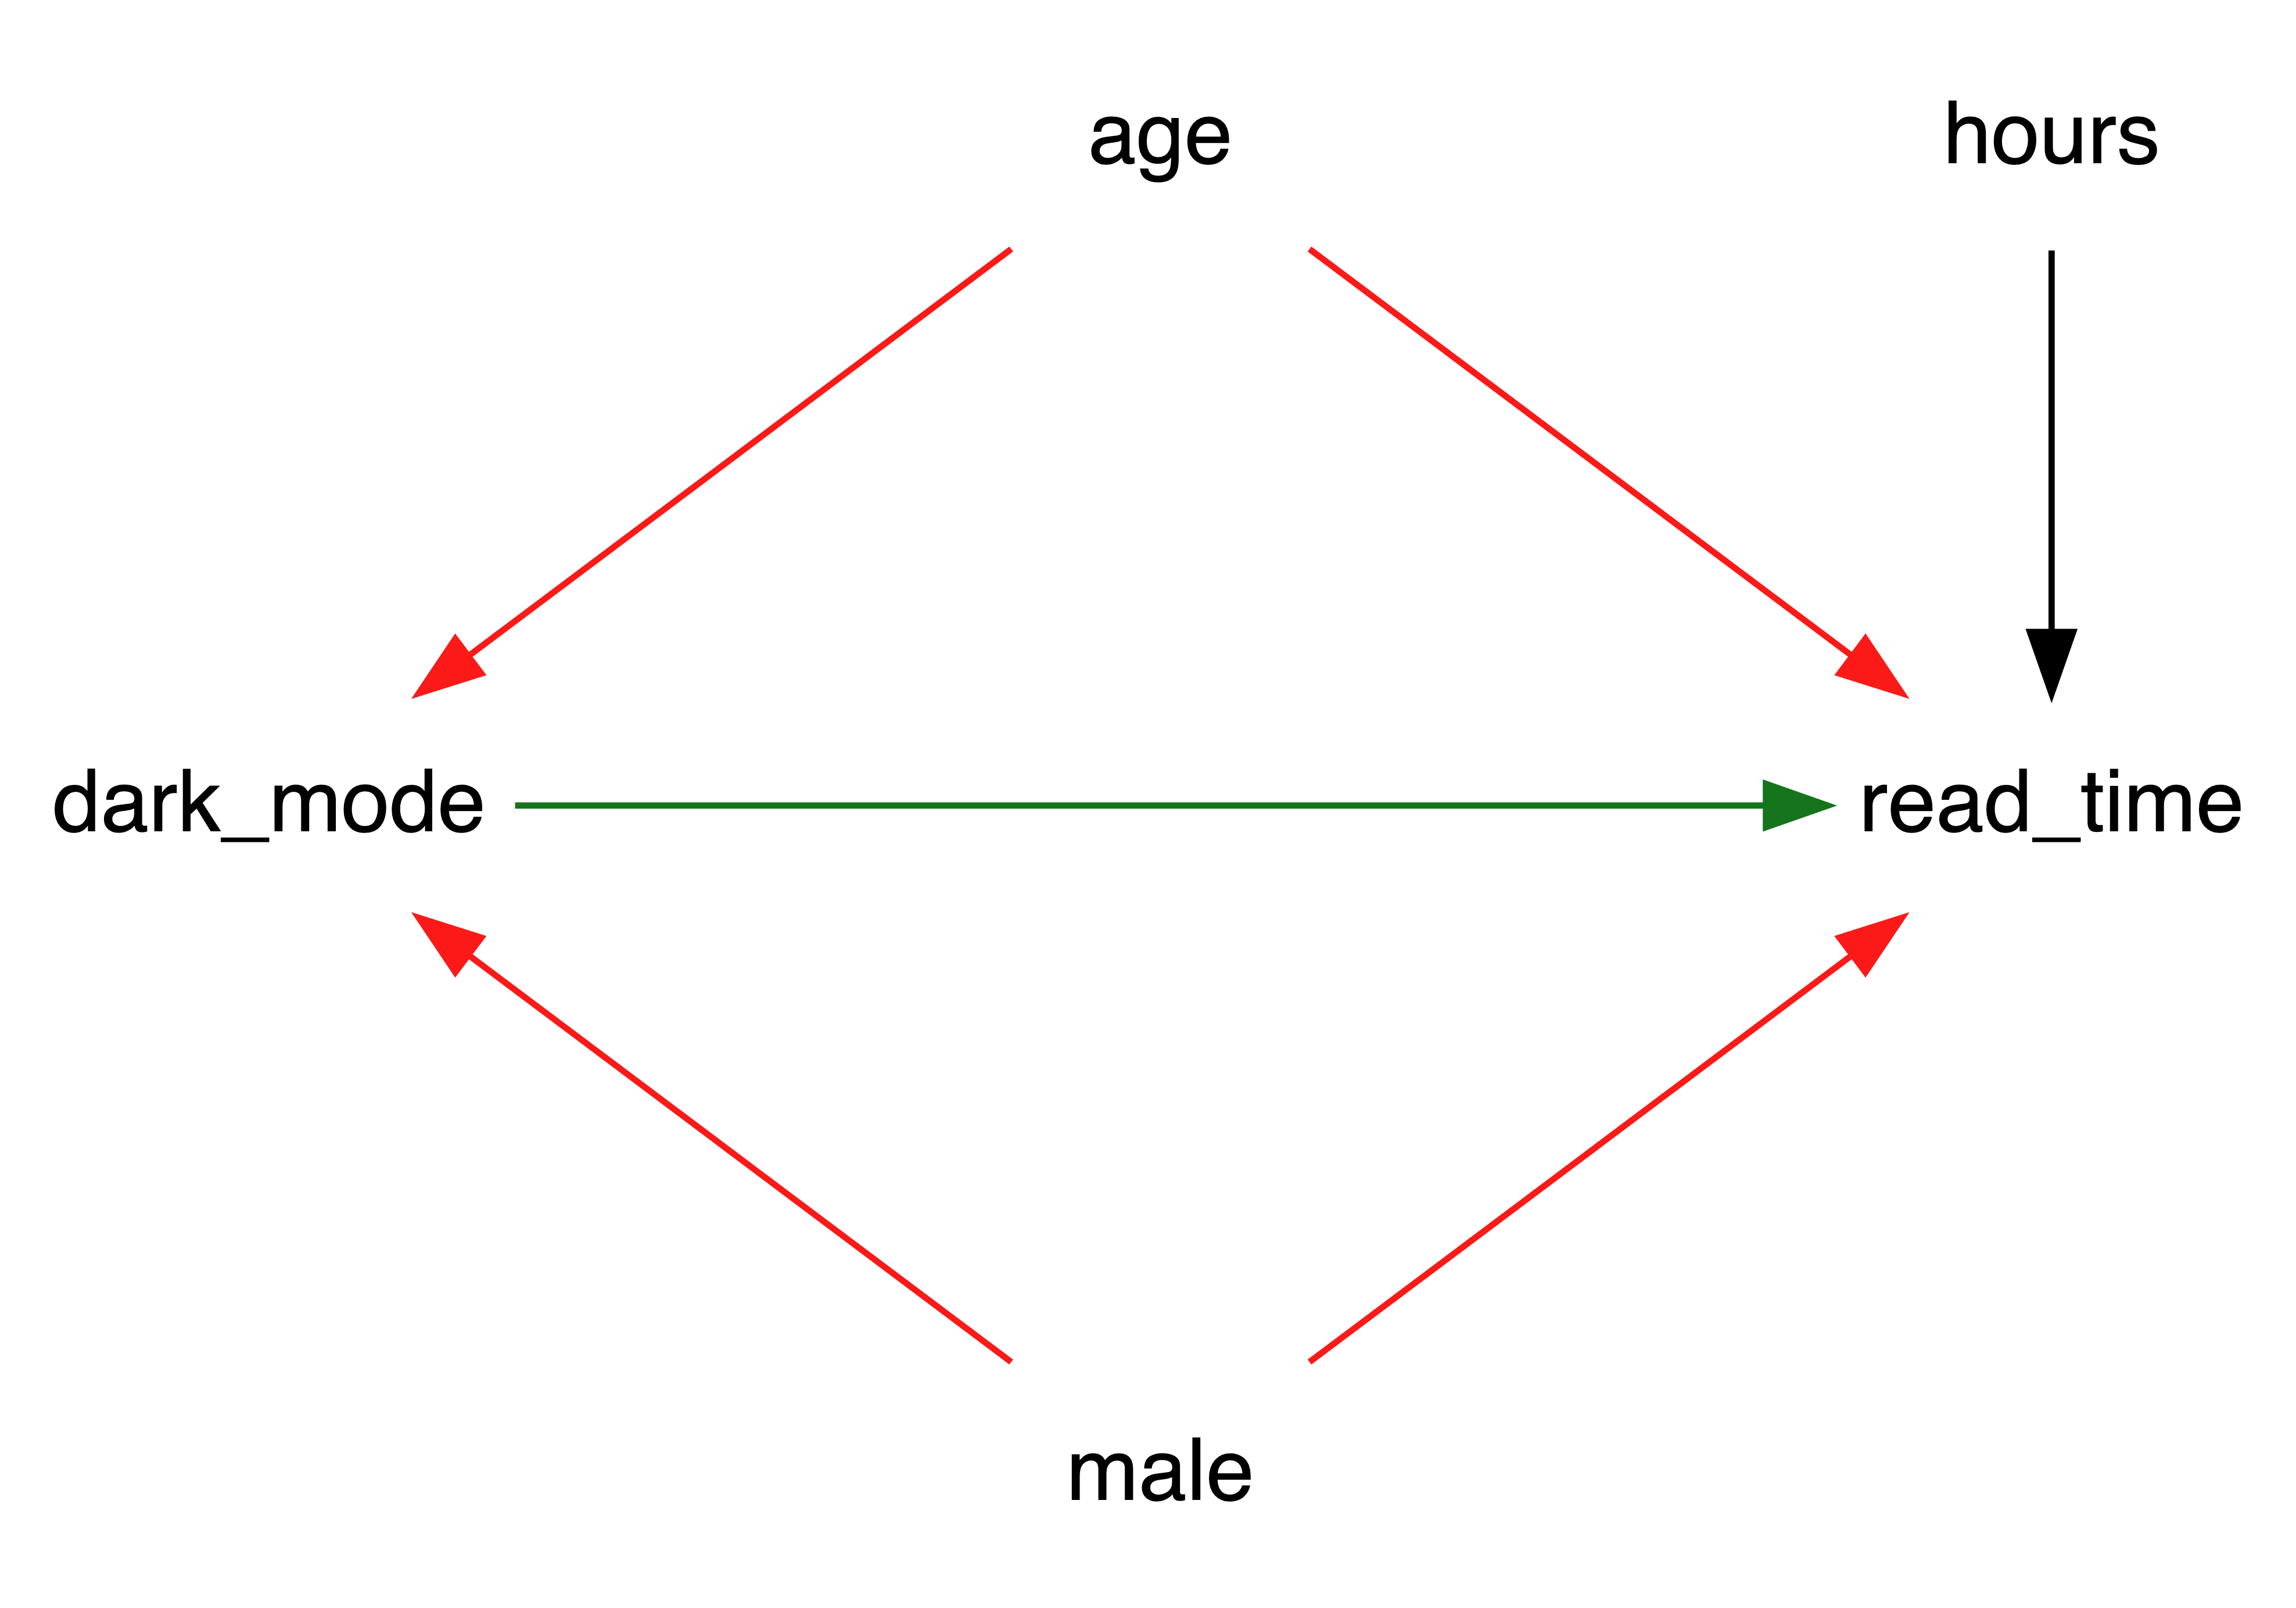
\includegraphics[width=4in,height=3in]{Matching_files/figure-latex/dot-figure-3.png}

}

\caption{\label{fig-CDdarkmode}Erweiterter DGP im
Website-Design-Beispiel}

\end{figure}%

Die Beurteilung der \emph{Balance} von Kontrollgruppe und
Behandlungsgruppe kann durch eine grafische Gegenüberstellung der
empirischen Verteilungen der Kovariablen beider Gruppen erfolgen. Wir
visualisieren die empirischen Verteilungen mit \texttt{ggplot2}. Hierzu
standardisieren wir \texttt{age} und \texttt{hours} zunächst mit
\texttt{scale()}.

\begin{Shaded}
\begin{Highlighting}[]
\CommentTok{\# Datensatz für graphische Darstellung formatieren}
\NormalTok{darkmode\_p }\OtherTok{\textless{}{-}}\NormalTok{ darkmode }\SpecialCharTok{\%\textgreater{}\%} 
  \CommentTok{\# Standardisierung mit \textquotesingle{}scale()\textquotesingle{}}
  \FunctionTok{mutate}\NormalTok{(}
    \AttributeTok{dark\_mode =} \FunctionTok{as\_factor}\NormalTok{(dark\_mode),}
    \AttributeTok{age =} \FunctionTok{scale}\NormalTok{(age), }
    \AttributeTok{hours =} \FunctionTok{scale}\NormalTok{(hours)}
\NormalTok{  )}

\FunctionTok{head}\NormalTok{(darkmode\_p)}
\end{Highlighting}
\end{Shaded}

\begin{verbatim}
# A tibble: 6 x 5
  read_time dark_mode  male age[,1] hours[,1]
      <dbl> <fct>     <dbl>   <dbl>     <dbl>
1      14.4 0             0  0.0377    -0.591
2      15.4 0             1  1.11      -0.459
3      20.9 1             0 -1.74       0.684
4      20   0             0 -0.141     -0.451
5      21.5 1             0 -1.21      -0.316
6      19.5 0             0  1.91      -0.327
\end{verbatim}

Für \texttt{age} und \texttt{hours} eignen sich die geschätzten
Dichtefunktionen für einen Vergleich der Verteilungen in Behandlungs-
und Kontrollgruppe.

\begin{Shaded}
\begin{Highlighting}[]
\CommentTok{\# Vergleich mit Dichteschätzungen}
\NormalTok{darkmode\_p }\SpecialCharTok{\%\textgreater{}\%}
  \FunctionTok{select}\NormalTok{(dark\_mode, hours, age) }\SpecialCharTok{\%\textgreater{}\%}
  \CommentTok{\# in langes Format überführen}
  \FunctionTok{pivot\_longer}\NormalTok{(}\AttributeTok{cols =} \FunctionTok{c}\NormalTok{(}\SpecialCharTok{{-}}\NormalTok{dark\_mode)) }\SpecialCharTok{\%\textgreater{}\%}
  
  \FunctionTok{ggplot}\NormalTok{(}
    \FunctionTok{aes}\NormalTok{(}\AttributeTok{x =}\NormalTok{ value, }\AttributeTok{fill =}\NormalTok{ dark\_mode)}
\NormalTok{    ) }\SpecialCharTok{+}
  \FunctionTok{geom\_density}\NormalTok{(}\AttributeTok{alpha =}\NormalTok{ .}\DecValTok{5}\NormalTok{) }\SpecialCharTok{+} 
  \FunctionTok{facet\_wrap}\NormalTok{(}
    \AttributeTok{facets =} \SpecialCharTok{\textasciitilde{}}\NormalTok{ name, }
    \AttributeTok{scales =} \StringTok{"free"}\NormalTok{, }
    \AttributeTok{nrow =} \DecValTok{2}
\NormalTok{    )}
\end{Highlighting}
\end{Shaded}

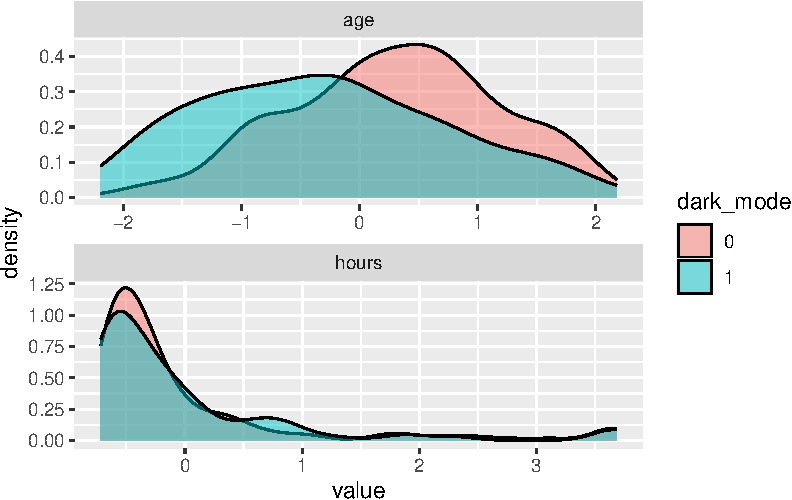
\includegraphics{Matching_files/figure-pdf/unnamed-chunk-14-1.pdf}

Die graphische Analyse zeigt deutliche Unterschiede in den Verteilungen
von \texttt{age} zwischen Kontroll- und Behandlungsgruppe. Für einen
Beurteilung mit deskriptiven Statistiken wird häufig eine sogenannte
\emph{Balance Table} herangezogen. Wir berechnen diese für \texttt{age},
\texttt{hours} und \texttt{male} mit \texttt{cobalt::bal.tab()}

\begin{Shaded}
\begin{Highlighting}[]
\FunctionTok{library}\NormalTok{(cobalt)}

\CommentTok{\# Balance table mit \textquotesingle{}cobalt::bal.tab()\textquotesingle{}}
\FunctionTok{bal.tab}\NormalTok{(}
  \AttributeTok{x =}\NormalTok{ darkmode }\SpecialCharTok{\%\textgreater{}\%} 
    \FunctionTok{select}\NormalTok{(age, hours, male), }
  \AttributeTok{treat =}\NormalTok{ darkmode}\SpecialCharTok{$}\NormalTok{dark\_mode, }
   \CommentTok{\# berechne SMD für KG und TG:}
  \AttributeTok{disp =} \StringTok{"m"}\NormalTok{, }
  \AttributeTok{s.d.denom =} \StringTok{"pooled"}
\NormalTok{)}
\end{Highlighting}
\end{Shaded}

\begin{verbatim}
Balance Measures
         Type   M.0.Un   M.1.Un Diff.Un
age   Contin.  46.0132  39.0940 -0.6469
hours Contin. 337.7775 328.5738 -0.0203
male   Binary   0.3377   0.6577  0.3200

Sample sizes
    Control Treated
All     151     149
\end{verbatim}

Die Einträge \texttt{M.0.Un} und \texttt{M.1.Un} zeigen die jeweiligen
Stichprobenmittelwerte der Variablen für Kontroll- und
Behandlungsgruppe. \texttt{Diff.Un} gibt eine standardisierte
Mittelwertdifferenz \(SMD\) an, wobei \begin{align*}
  SMD_j := \left(\overline{X}_{j,B} - \overline{X}_{j,K}\right) \bigg/ \sqrt{\frac{1}{2}\left(\widehat{\text{Var}}(X_{j,B}) + \widehat{\text{Var}}(X_{j,K})\right)},
\end{align*} mit Stichprobenmitteln \(\overline{X}_{j,B}\) und
\(\overline{X}_{j,K}\) und Stichprobenvarianzen
\(\widehat{\text{Var}}(X_{j,B})\) und \(\widehat{\text{Var}}(X_{j,K})\)
für eine kontinuierliche Kovariable \(j\).\footnote{Siehe P. Austin
  (2011) für einen Überblick zu Balance-Statistiken.} Obwohl es keinen
einheitlichen Schwellenwert für die standardisierte Differenz gibt, der
ein erhebliches Ungleichgewicht anzeigt, gilt für kontinuierliche
Variablen eine standardisierte (absolute) Differenz von weniger als
\(0.1\) als Hinweis auf einen vernachlässigbaren Unterschied zwischen
den Gruppen.

Die Balance Table weist also auf einen vernachlässigbaren Unterschied
für \texttt{hours} hin und bestätigt den aus den Grafiken abgeleiteten
Eindruck einer relevanten Differenzen für \texttt{age}.

\subsection{Entropy Balancing}\label{entropy-balancing}

\emph{Entropy Balancing} (Hainmueller 2012) ist eine weitere Methode zur
Gewährleistung der Vergleichbarkeit von Behandlungs- und Kontrollgruppe
anhand von Gewichten. Das Verfahren nutzt Konzepte aus der
\href{https://de.wikipedia.org/wiki/Informationstheorie}{Informationstheorie}
um die Gewichte für Subjekte in der Kontrollgruppe so anzupassen, dass
die Verteilung der Matchingvariablen in der Kontrollgruppe die
Verteilung in der Behandlungsgruppe möglichst gut approximiert. Dies
geschieht unter der Restriktion, dass bestimmte empirische Momente
(meist Mittelwerte und Varianzen) der Matchingvariablen exakt
übereinstimmen. Mathematisch werden die Gewichte für
Kontrollgruppenbeobachtungen durch Minimierung der
\href{https://de.wikipedia.org/wiki/Kullback-Leibler-Divergenz}{Kullback-Leibler-Divergenz}
zwischen den Verteilungen gefunden, wobei die Divergenz ein Maß für den
Unterschied von Wahrscheinlichkeitsverteilungen ist.

Entropy Balancing ist im R-Paket \texttt{WeightIt} implementiert. Wir
zeigen, wie die benötigten Gewichte für eine Schätzungen des ATT im
Website-Beispiel mit \texttt{WeightIt::wightit()} bestimmt werden
können. Über das Argument \texttt{moments} legen wir fest, dass die
Gewichte unter der Restriktion übereinstimmender Mittelwerte aller
Matching-Variablen zwischen Behandlungs- und Kontrollgruppe erfolgen
soll.

\begin{Shaded}
\begin{Highlighting}[]
\FunctionTok{library}\NormalTok{(WeightIt)}

\CommentTok{\# Gewichte für Entropy Balancing}
\NormalTok{(}
\NormalTok{  W1 }\OtherTok{\textless{}{-}} \FunctionTok{weightit}\NormalTok{(}
\NormalTok{  dark\_mode }\SpecialCharTok{\textasciitilde{}}\NormalTok{ age }\SpecialCharTok{+}\NormalTok{ male }\SpecialCharTok{+}\NormalTok{ hours,}
  \AttributeTok{data =}\NormalTok{ darkmode,}
  \AttributeTok{method =} \StringTok{"ebal"}\NormalTok{, }
  \AttributeTok{estimand =} \StringTok{"ATT"}\NormalTok{,}
  \AttributeTok{moments =} \DecValTok{1}
\NormalTok{  )}
\NormalTok{ )}
\end{Highlighting}
\end{Shaded}

\begin{verbatim}
A weightit object
 - method: "ebal" (entropy balancing)
 - number of obs.: 300
 - sampling weights: none
 - treatment: 2-category
 - estimand: ATT (focal: 1)
 - covariates: age, male, hours
\end{verbatim}

Wir schätzen den Behandlungseffekt nach Entropy Balancing mit
gewichteter Regression.

\begin{Shaded}
\begin{Highlighting}[]
\CommentTok{\# Mittelwert{-}Vergleich mit lm()}
\NormalTok{fit }\OtherTok{\textless{}{-}} \FunctionTok{lm}\NormalTok{(}
  \AttributeTok{formula =}\NormalTok{ read\_time }\SpecialCharTok{\textasciitilde{}}\NormalTok{ dark\_mode, }
  \AttributeTok{data =}\NormalTok{ darkmode, }
  \AttributeTok{weights =}\NormalTok{ W1}\SpecialCharTok{$}\NormalTok{weights}
\NormalTok{)}
\FunctionTok{summary}\NormalTok{(fit)}
\end{Highlighting}
\end{Shaded}

\begin{verbatim}

Call:
lm(formula = read_time ~ dark_mode, data = darkmode, weights = W1$weights)

Weighted Residuals:
     Min       1Q   Median       3Q      Max 
-16.6652  -2.3552   0.8786   2.9585  27.1808 

Coefficients:
            Estimate Std. Error t value Pr(>|t|)    
(Intercept)  17.7601     0.4093  43.395   <2e-16 ***
dark_mode     0.9701     0.5807   1.671   0.0959 .  
---
Signif. codes:  0 '***' 0.001 '**' 0.01 '*' 0.05 '.' 0.1 ' ' 1

Residual standard error: 5.029 on 298 degrees of freedom
Multiple R-squared:  0.009278,  Adjusted R-squared:  0.005953 
F-statistic: 2.791 on 1 and 298 DF,  p-value: 0.09586
\end{verbatim}

Beachte, dass die von \texttt{summary()} berechneten Standardfehler bei
Entropy Balancing ungültig sind. In Abschnitt
Kapitel~\ref{sec-bootmatching} erläutern wir die Berechnung von
Standardfehlern für Matching-Schätzer mit dem Bootstrap.

\subsection{Mehrere Matching-Variablen und der Propensity
Score}\label{sec-PSM}

Bei mehreren Backdoor-Variablen kann eine Gewichtung anhand der
Behandlungswahrscheinlichkeit (\emph{Treatment Propensity}) erfolgen.
Die Idee hierbei ist, dass der DGP wie in
Abbildung~\ref{fig-propCDdarkmode} dargestellt werden kann.

\begin{figure}[t]

\centering{

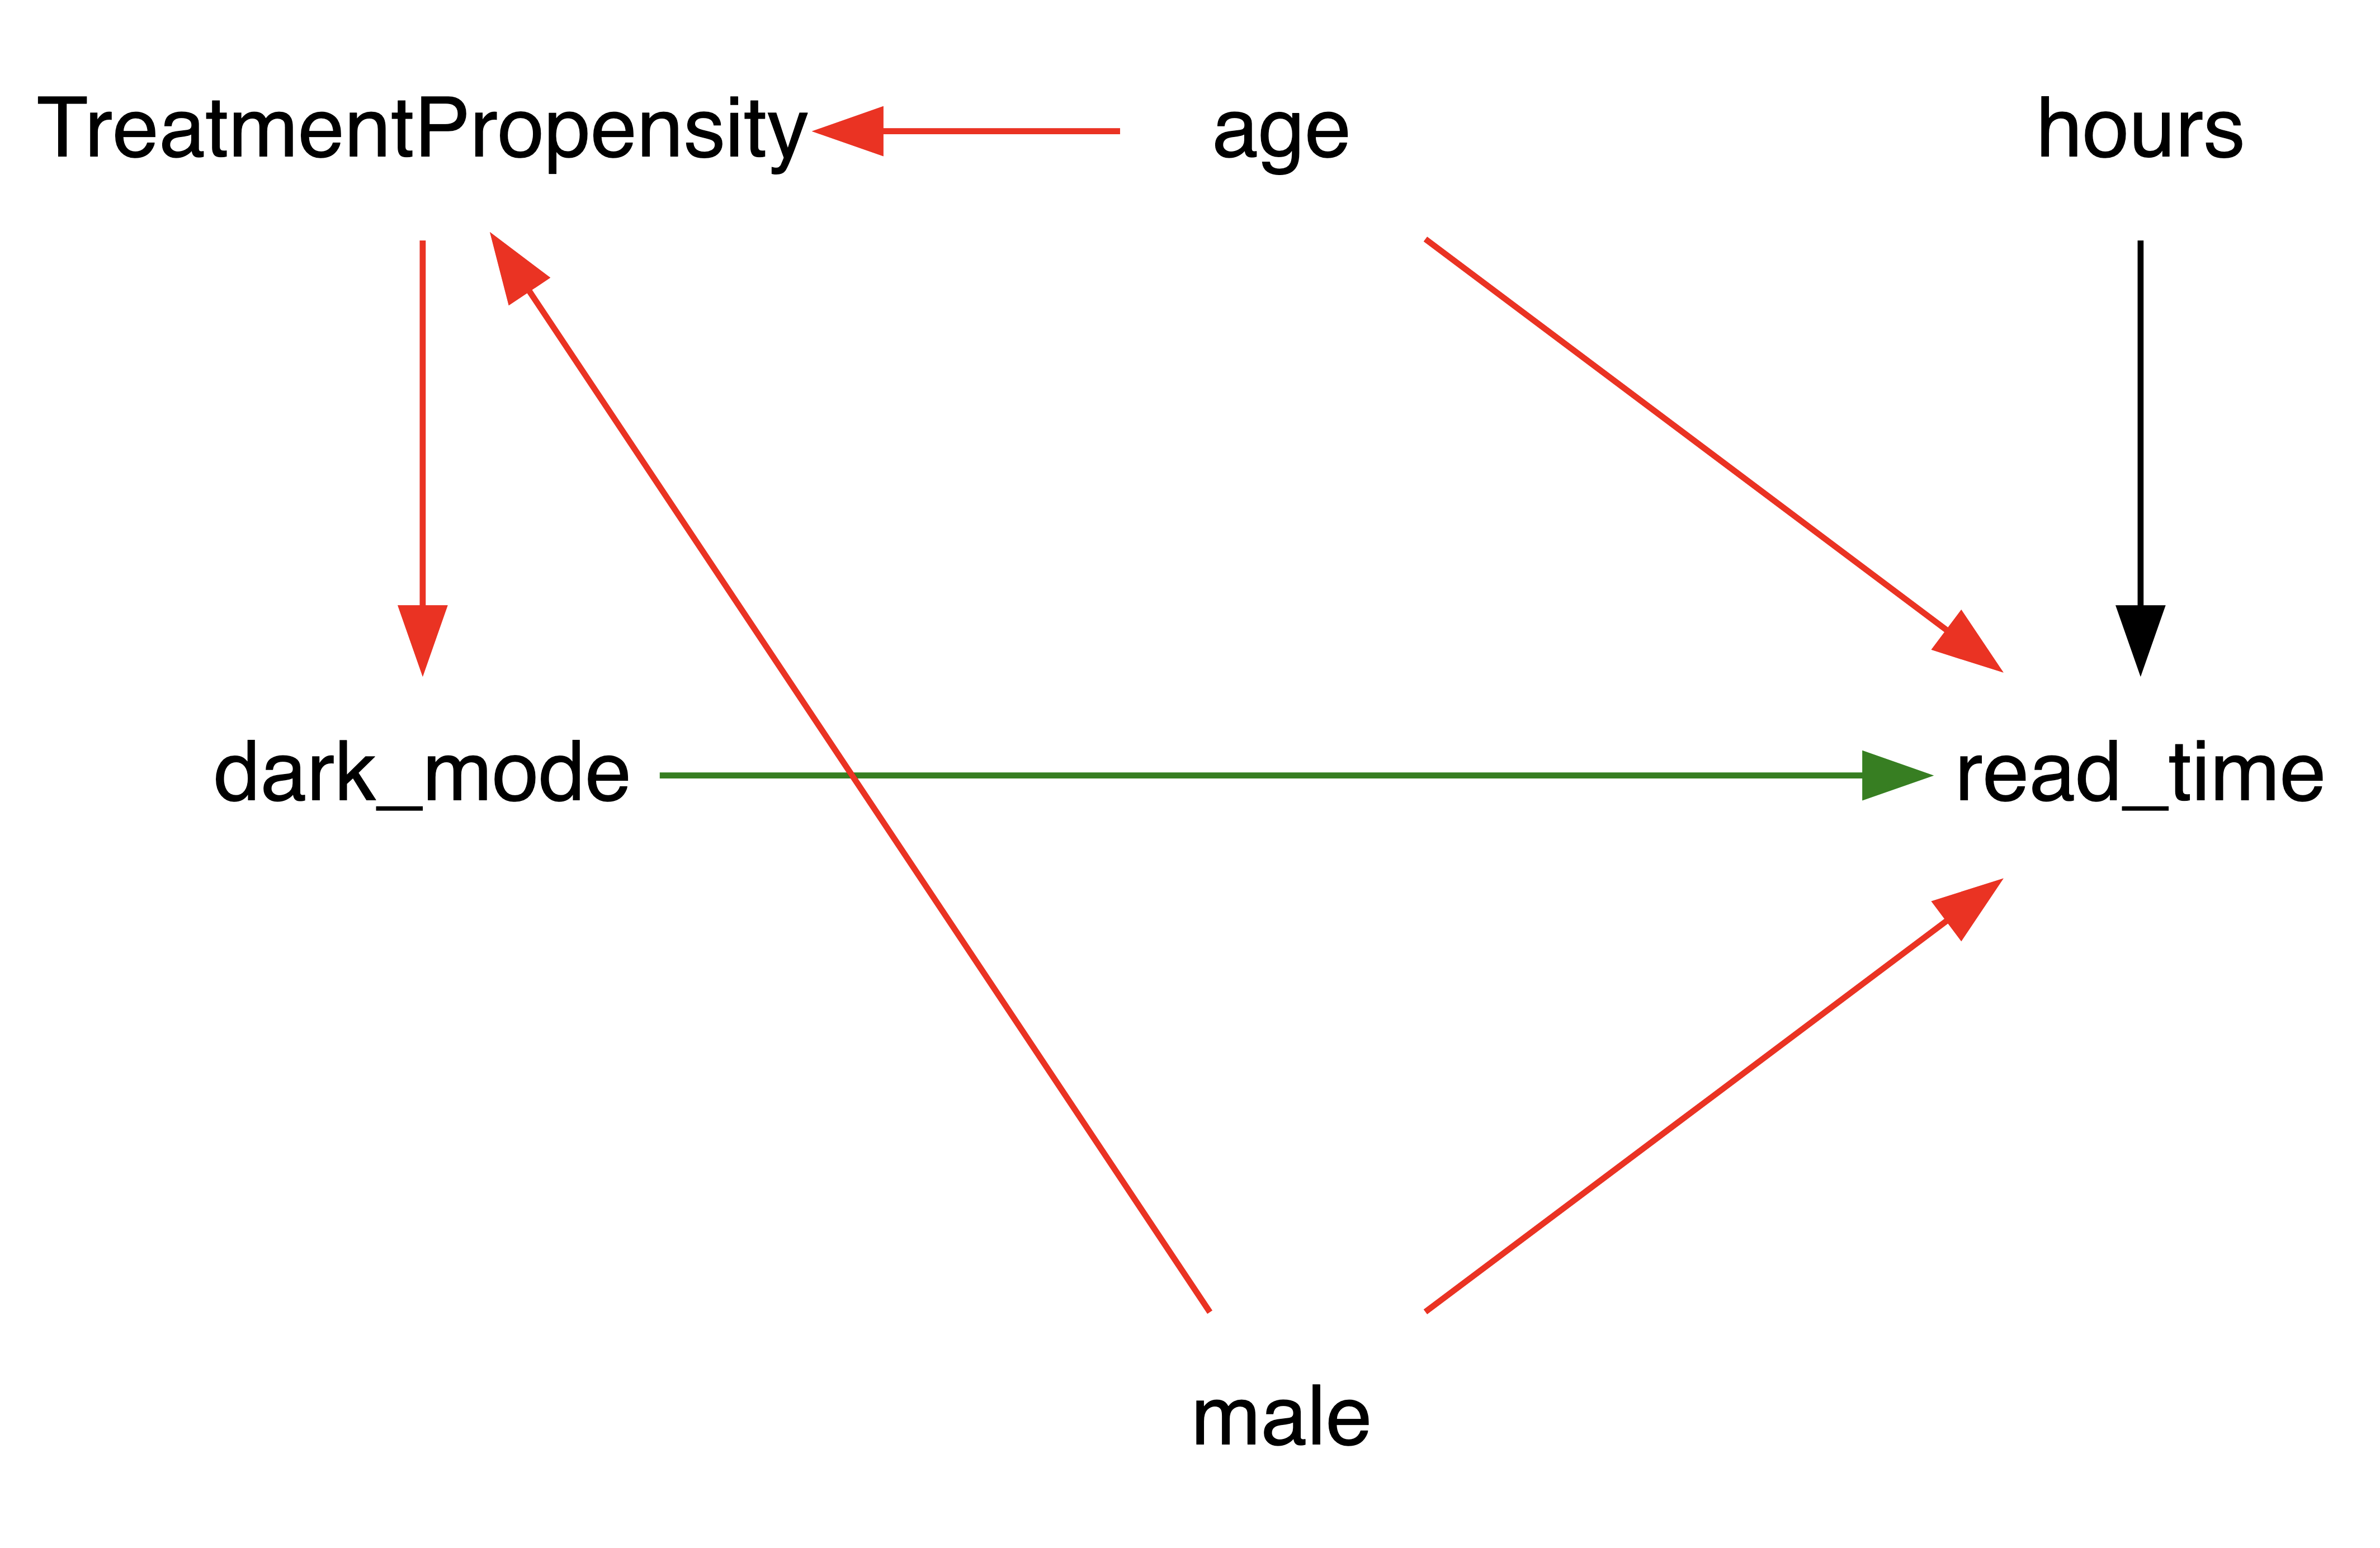
\includegraphics[width=4in,height=3in]{Matching_files/figure-latex/dot-figure-2.png}

}

\caption{\label{fig-propCDdarkmode}Propensity im
Website-Design-Beispiel}

\end{figure}%

Hierbei beeinflussen die Backdoor-Variablen \emph{age} und \emph{male}
die Behandlungsvariable \emph{dark\_mode} lediglich durch die
Behandlungswahrscheinlichkeit \emph{Treatment Propensity}. Diese
Darstellung zeigt, das die mehrdimensionale Information bzgl. der
Ähnlichkeit von Subjekten hinsichtlich der beobachteten Kovariablen in
einer einzigen Variable zusammengefasst werden kann. Die Backdoor-Pfade
können daher geschlossen werden, indem wir Subjekte anhand von
\emph{Treatment Propensity} derart gewichten, dass beide Gruppen
hinsichtlich der Verteilung der Behandlungswahrscheinlichkeit
vergleichbar sind. Betrachte erneut \eqref{eq:cia} und beachte, dass
\begin{align}
  Y_i = Y_i^{(1)} D_i + Y_i^{(0)} (1-D_i).
\end{align} Rosenbaum und Rubin (1983) zeigen, dass es hinsichtlich
\eqref{eq:cia} äquivalent ist für die \emph{Treatment Propensity}
\(P_i(X_i):=P(B_i=1\vert X_i = x)\) zu kontrollieren, d.h. \begin{align}
  \left\{Y_i^{(1)},Y_i^{(0)}\right\} \perp B_i\vert X_i \quad\Leftrightarrow\quad \left\{Y_i^{(1)},Y_i^{(0)}\right\} \perp B_i\vert P_i(X_i).
\end{align}

Der Behandlungseffekt kann so als Differenz von gewichteten
Gruppenmittelwerten berechnet werden, mit inversem
Wahrscheinlichkeitsgewicht (IPW) \(w_{i,B} = 1/P_i(X_i)\) für
Beobachtungen in der Behandlungsgruppe und \(w_{i,K} = 1/(1-P_i(X_i))\)
für Beobachtungen in der Kontrollgruppe, \begin{align}
  \tau^{\text{IPW}} = \frac{1}{n}\sum_{i=1}^n \left[\frac{B_i Y_i}{P_i(X_i)} - \frac{(1-B_i)Y_i}{1-P_i(X_i)} \right].\label{eq:tauipw}
\end{align}

Grundsätzlich ist \emph{TreatmentPropensity} eine nicht beobachtbare
Variable und muss daher aus den Daten geschätzt werden. Eine geschätzte
Behandlungswahrscheinlichkeiten \(\widehat{P}_i(X_i)\) wird als
\emph{Propensity Score} bezeichnet. In der Praxis erfolgt die Schätzung
von \emph{Propensity Scores} meist mit logistischer Regression. Ein
erwartungstreuer Schätzer des ATE ist \begin{align}
  \widehat{\tau}^{\text{IPW}} = \frac{1}{n}\sum_{i=1}^n \left[\frac{B_i Y_i}{\widehat{P}_i(X_i)} - \frac{(1-B_i)Y_i}{1-\widehat{P}_i(X_i)} \right].\label{eq:hattauipw}
\end{align} Hirano, Imbens, und Ridder (2003) diskutieren Alternativen
zu \eqref{eq:hattauipw} für die Schätzung anderer Typen von
Behandlungseffekten.

Wir schätzen nachfolgend die \emph{Propensity Scores} für unser
Anwendungsbeispiel, erläutern die Berechnung der Gewichte sowie die
Schätzung von Behandlungseffekten mit gewichteter Regression. Hierbei
betrachten wir eine Variante von \eqref{eq:hattauipw} mit normalisierten
Gewichten \(\tilde{w}_{i,B} = w_{i,B}/\sum_i w_{i,B}\) und
\(\tilde{w}_{i,K} = w_{i,K}/\sum_i w_{i,K}\) die sich jeweils zu 1
summieren.\footnote{Eine Normalisierung der Gewichte reduziert die
  Varianz des Schätzers, vgl. Hirano, Imbens, und Ridder (2003)} Dies
ergibt den Hájek-Schätzer\footnote{Siehe Hájek (1971).} \begin{align}
    \widehat{\tau}_N^{\text{IPW}} = \frac{\sum_i\tilde{w}_{i,B}Y_i}{\sum_i\tilde{w}_{i,B}} -  \frac{\sum_i\tilde{w}_{i,K}Y_i}{\sum_i\tilde{w}_{i,K}}.\label{eq:hattauhajek}
\end{align}

Zunächst Schätzen wir ein logistisches Regressionsmodell mit
\texttt{age}, \texttt{male} und \texttt{hours} als erklärende Variablen
für \texttt{dark\_mode}.

\begin{Shaded}
\begin{Highlighting}[]
\CommentTok{\# Logit{-}Modell mit \textquotesingle{}glm()\textquotesingle{} schätzen}
\NormalTok{(}
\NormalTok{  darkmode\_ps\_logit }\OtherTok{\textless{}{-}} \FunctionTok{glm}\NormalTok{(}
    \AttributeTok{formula =}\NormalTok{ dark\_mode }\SpecialCharTok{\textasciitilde{}}\NormalTok{ age }\SpecialCharTok{+}\NormalTok{ male }\SpecialCharTok{+}\NormalTok{ hours,}
    \AttributeTok{data =}\NormalTok{ darkmode,}
    \AttributeTok{family =}\NormalTok{ binomial}
\NormalTok{  )}
\NormalTok{)}
\end{Highlighting}
\end{Shaded}

\begin{verbatim}

Call:  glm(formula = dark_mode ~ age + male + hours, family = binomial, 
    data = darkmode)

Coefficients:
(Intercept)          age         male        hours  
  2.330e+00   -7.330e-02    1.623e+00   -9.293e-05  

Degrees of Freedom: 299 Total (i.e. Null);  296 Residual
Null Deviance:      415.9 
Residual Deviance: 346.4    AIC: 354.4
\end{verbatim}

Die \emph{Propensity Scores} erhalten wir als angepasste Werte aus der
Regression \texttt{darkmode\_ps\_logit} mit \texttt{fitted()}. Wir
erweitern den Datensatz mit den Ergebnissen.

\begin{Shaded}
\begin{Highlighting}[]
\CommentTok{\# Datensatz um Propensity Scores erweitern}
\NormalTok{(}
\NormalTok{  darkmode\_probs }\OtherTok{\textless{}{-}} 
\NormalTok{    darkmode }\SpecialCharTok{\%\textgreater{}\%}
    \FunctionTok{mutate}\NormalTok{(}
      \AttributeTok{PS =} \FunctionTok{fitted}\NormalTok{(darkmode\_ps\_logit)}
\NormalTok{    )}
\NormalTok{)}
\end{Highlighting}
\end{Shaded}

\begin{verbatim}
# A tibble: 300 x 6
   read_time dark_mode  male   age  hours     PS
       <dbl>     <dbl> <dbl> <dbl>  <dbl>  <dbl>
 1      14.4         0     0    43   65.6 0.304 
 2      15.4         0     1    55  125.  0.478 
 3      20.9         1     0    23  643.  0.642 
 4      20           0     0    41  129.  0.335 
 5      21.5         1     0    29  190.  0.547 
 6      19.5         0     0    64  185.  0.0849
 7      22           1     0    18  334.  0.727 
 8      17.4         0     0    53  279.  0.171 
 9      23.6         0     0    59 1303.  0.108 
10      15.7         0     0    53   16.1 0.174 
# i 290 more rows
\end{verbatim}

Zur Beurteilung der Überlappung (vgl. Annahme \eqref{eq:overlap} können
wir die Verteilung der \emph{Propensity Scores} nach
Behandlungs-Indikator mit Histogrammen visualisieren.

\begin{Shaded}
\begin{Highlighting}[]
\CommentTok{\# Überlappung prüfen:}
\CommentTok{\# Histogramme der PS nach Treatment{-}Indikator}
\NormalTok{darkmode\_probs }\SpecialCharTok{\%\textgreater{}\%}
  \FunctionTok{ggplot}\NormalTok{(}
    \AttributeTok{mapping =} \FunctionTok{aes}\NormalTok{(}
      \AttributeTok{x =}\NormalTok{ PS, }
      \AttributeTok{fill =} \FunctionTok{factor}\NormalTok{(dark\_mode)}
\NormalTok{    )}
\NormalTok{  ) }\SpecialCharTok{+} 
  \FunctionTok{geom\_histogram}\NormalTok{(}
    \AttributeTok{alpha =}\NormalTok{ .}\DecValTok{5}\NormalTok{, }
    \AttributeTok{bins =} \DecValTok{25}\NormalTok{, }
    \AttributeTok{position =} \StringTok{"identity"}
\NormalTok{  )}
\end{Highlighting}
\end{Shaded}

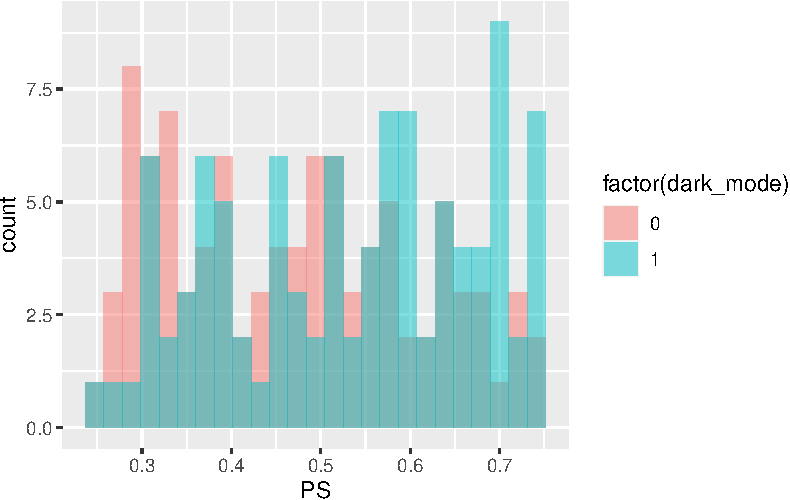
\includegraphics{Matching_files/figure-pdf/unnamed-chunk-21-1.pdf}

Ein Vergleich der Histogramme zeigt, dass die Überlappung der
\emph{Propensity Scores} in der linken Flanken der Verteilungen der
Kontrollgruppe und in der rechten Flanke der Behandlungsgruppe
schlechter wird. Wir entfernen zunächst Beobachtungen aus der Stichprobe
deren \emph{Propensity Scores} wenig bzw. keine Überlappung aufweisen.

\begin{Shaded}
\begin{Highlighting}[]
\CommentTok{\# Datensatz nach PS trimmen}
\NormalTok{darkmode\_probs }\OtherTok{\textless{}{-}}\NormalTok{ darkmode\_probs }\SpecialCharTok{\%\textgreater{}\%} 
  \FunctionTok{filter}\NormalTok{(}
    \FunctionTok{between}\NormalTok{(}
      \AttributeTok{x =}\NormalTok{ PS,}
      \AttributeTok{left =}\NormalTok{ .}\DecValTok{25}\NormalTok{,}
      \AttributeTok{right =}\NormalTok{ .}\DecValTok{75}
\NormalTok{    )}
\NormalTok{  )}
\end{Highlighting}
\end{Shaded}

\begin{Shaded}
\begin{Highlighting}[]
\CommentTok{\# Überlappung nach trimming prüfen:}
\CommentTok{\# Dichteschätzung der PS nach Treatment{-}Indikator}
\NormalTok{darkmode\_probs }\SpecialCharTok{\%\textgreater{}\%}
\FunctionTok{ggplot}\NormalTok{(}
  \AttributeTok{mapping =} \FunctionTok{aes}\NormalTok{(}
    \AttributeTok{x =}\NormalTok{ PS, }
    \AttributeTok{fill =} \FunctionTok{factor}\NormalTok{(dark\_mode))}
\NormalTok{  ) }\SpecialCharTok{+} 
  \FunctionTok{geom\_histogram}\NormalTok{(}
    \AttributeTok{alpha =}\NormalTok{ .}\DecValTok{5}\NormalTok{, }
    \AttributeTok{bins =} \DecValTok{25}\NormalTok{, }
    \AttributeTok{position =} \StringTok{"identity"}
\NormalTok{  )}
\end{Highlighting}
\end{Shaded}

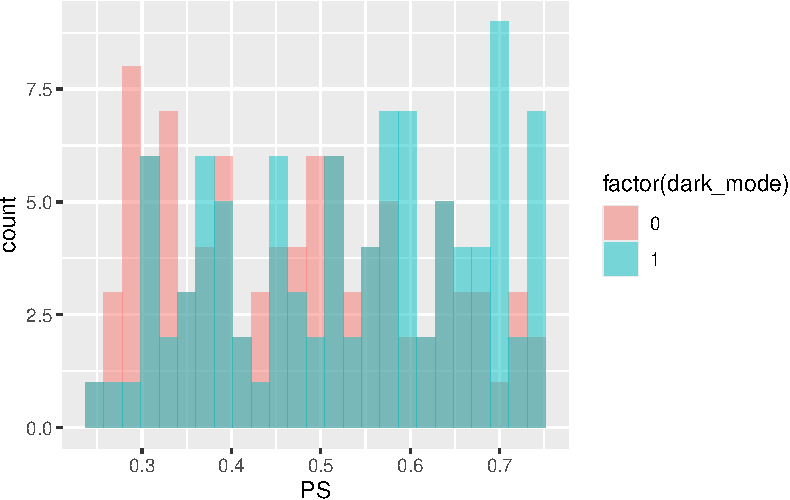
\includegraphics{Matching_files/figure-pdf/unnamed-chunk-23-1.pdf}

IPWs anhand der \emph{Propensity Scores} können schnell mit der
Vorschrift \begin{align}
  \text{IPW} = \frac{\text{dark\_mode}}{\text{PS}} + \frac{1 - \text{dark\_mode}}{1 - \text{PS}},
\end{align} berechnet werden.

\begin{Shaded}
\begin{Highlighting}[]
\CommentTok{\# Datensatz um IPWs erweitern}
\NormalTok{darkmode\_IPW }\OtherTok{\textless{}{-}}\NormalTok{ darkmode\_probs }\SpecialCharTok{\%\textgreater{}\%}
  \FunctionTok{mutate}\NormalTok{(}
    \AttributeTok{IPW =}\NormalTok{ dark\_mode }\SpecialCharTok{/}\NormalTok{ PS }\SpecialCharTok{+}\NormalTok{ (}\DecValTok{1} \SpecialCharTok{{-}}\NormalTok{ dark\_mode) }\SpecialCharTok{/}\NormalTok{ (}\DecValTok{1} \SpecialCharTok{{-}}\NormalTok{ PS)}
\NormalTok{  )}

\NormalTok{darkmode\_IPW }\SpecialCharTok{\%\textgreater{}\%} 
  \FunctionTok{select}\NormalTok{(IPW)}
\end{Highlighting}
\end{Shaded}

\begin{verbatim}
# A tibble: 194 x 1
     IPW
   <dbl>
 1  1.44
 2  1.91
 3  1.56
 4  1.50
 5  1.83
 6  1.38
 7  1.43
 8  1.47
 9  2.71
10  1.42
# i 184 more rows
\end{verbatim}

Eine Schätzung des durchschnittlichen Behandlungseffekts gemäß
\eqref{eq:hattauhajek} implementieren wir mit \texttt{dplyr}.

\begin{Shaded}
\begin{Highlighting}[]
\NormalTok{darkmode\_IPW }\SpecialCharTok{\%\textgreater{}\%}
  \FunctionTok{group\_by}\NormalTok{(dark\_mode) }\SpecialCharTok{\%\textgreater{}\%}
  \FunctionTok{mutate}\NormalTok{(}\AttributeTok{w =}\NormalTok{ IPW }\SpecialCharTok{/} \FunctionTok{sum}\NormalTok{(IPW)) }\SpecialCharTok{\%\textgreater{}\%}
  \FunctionTok{summarise}\NormalTok{(}\AttributeTok{weighted\_mean =} \FunctionTok{sum}\NormalTok{(read\_time }\SpecialCharTok{*}\NormalTok{ w)) }\SpecialCharTok{\%\textgreater{}\%}
  \FunctionTok{summarise}\NormalTok{(}\AttributeTok{diff =} \FunctionTok{diff}\NormalTok{(weighted\_mean))}
\end{Highlighting}
\end{Shaded}

\begin{verbatim}
# A tibble: 1 x 1
   diff
  <dbl>
1  1.90
\end{verbatim}

Diese Schätzung des Behandlungseffekts ist äquivalent zur gewichteten
KQ-Schätzung anhand eines einfachen linearen Regressionsmodells.

\begin{Shaded}
\begin{Highlighting}[]
\CommentTok{\# Mit IPWs gewichteter KQ{-}Schaetzer berechnet den ATE}
\NormalTok{model\_ipw }\OtherTok{\textless{}{-}} \FunctionTok{lm}\NormalTok{(}
  \AttributeTok{formula =}\NormalTok{ read\_time }\SpecialCharTok{\textasciitilde{}}\NormalTok{ dark\_mode, }
  \AttributeTok{data =}\NormalTok{ darkmode\_IPW,}
  \AttributeTok{weights =}\NormalTok{ IPW}
\NormalTok{)}

\FunctionTok{summary}\NormalTok{(model\_ipw)}
\end{Highlighting}
\end{Shaded}

\begin{verbatim}

Call:
lm(formula = read_time ~ dark_mode, data = darkmode_IPW, weights = IPW)

Weighted Residuals:
     Min       1Q   Median       3Q      Max 
-18.5086  -4.4579   0.6096   4.1345  20.4566 

Coefficients:
            Estimate Std. Error t value Pr(>|t|)    
(Intercept)  17.9709     0.4942  36.362  < 2e-16 ***
dark_mode     1.9011     0.6952   2.735  0.00683 ** 
---
Signif. codes:  0 '***' 0.001 '**' 0.01 '*' 0.05 '.' 0.1 ' ' 1

Residual standard error: 6.913 on 192 degrees of freedom
Multiple R-squared:  0.03749,   Adjusted R-squared:  0.03248 
F-statistic: 7.478 on 1 and 192 DF,  p-value: 0.006829
\end{verbatim}

Unsere Schätzung des ATE ist der geschätzte Koeffizient von
\texttt{dark\_mode}. Die ausgegebenen Standardfehler und
Inferenzstatistiken sind jedoch \emph{ungültig} aufgrund der Gewichtung
mit IPWs, den inversen \emph{geschätzten} Wahrscheinlichkeiten für eine
Behandlung. Der Grund hierfür ist, dass die Berechnung der
Standardfehler in \texttt{summary()} die zusätzliche Unsicherheit durch
die geschätzen \emph{Propensity Scores} nicht berücksichtigt! Später im
Kapitel erläutern wir die Berechnung gültiger Standardfehler für
IPW-Schätzer basierend auf \emph{Propensity Scores} mit dem Bootstrap.

\section{Selektierende
Matching-Verfahren}\label{selektierende-matching-verfahren}

Das grundsätzliche Konzept von selektierendem Matching wird in der
nachstehenden interaktiven Grafik veranschaulicht. Hier betrachten wir
beobachtete Ausprägungen von zwei (unabhängig und identisch verteilten)
Matching-Variablen für Subjekte in der Behandlungsgruppe (blau) sowie
Kontrollgruppe (rot). Als Matches qualifizieren sich sämtliche
Beobachtungen der anderen Gruppe, deren
\href{https://de.wikipedia.org/wiki/Euklidischer_Abstand}{Euklidische
Distanz} zu dem ausgewählten Punkt das über den Slider eingestellte
Maximum \emph{Caliper} nicht überschreitet.\footnote{Es handelt sich
  hierbei um einen Spezialfall von Matching anhand der
  Mahalanobis-Distanz.} Diese Region wird durch den gestrichelten Kreis
gekennzeichnet und kann über den zugehörigen Slider angepasst werden.
Per Klick auf eine Beobachtung werden Matches aus der anderen Gruppe
durch eine verbindende Linie und farbliches Hervorheben kenntlich
gemacht. Mit dem Slider für k wird festgelegt, dass nur die nahesten k
qualifizierten Beobachtungen als Matches behandelt werden. Die Grafik
illustriert inbesondere, dass Beobachtungen in Abhängigkeit von k und
Caliper falls gewünscht mehrfach (s.g. Matching mit Zurücklegen) oder
gar nicht gematcht werden können.

Für die nachfolgenden Code-Beispiele verwenden wir das R-Paket
\texttt{MatchIt}. \texttt{MatchIt::matchit()} nutzt standardmäßig
Eins-zu-Eins-Matching (ohne Zurücklegen) von Beobachtungen der
Treatment-Gruppe mit Beobachtungen der Kontrollgruppe.\footnote{Dieses
  Schema zielt auf eine Schätzung des ATT ab.} Die für das Matching zu
verwendenden Variablen werden über das Argument \texttt{formula} als
Funktion des Behandlungsindikators definiert. \texttt{matchit()}
bereitet das Objekt für eine Schätzung des ATT mit einer geeigneten
Funktionen, s. \texttt{?matchit} und hier insb. die Erläuterungen der
Argumente \texttt{replace\ =\ F}, \texttt{ratio\ =\ 1} und
\texttt{estimand\ =\ "ATT"} für Details. Mit \texttt{cobalt::balt.tab()}
erhalten wir eine \emph{balance table} für den gematchten Datensatz.

Wir zeigen als nächstes, wie \texttt{MatchIt::matchit()} für Matching
anhand der Regressoren \texttt{age}, \texttt{hours}, und \texttt{male}
in unserem Website-Beispiel für unterschiedliche Varianten durchgeführt
werden kann.

\subsection{Exaktes Matching}\label{exaktes-matching}

Exaktes Matching ordnet einem Subjekt aus der Behandlungsgruppe ein oder
mehrere Subjekte aus der Kontrollgruppe zu, wenn die boebachteten
Ausprägung der Matching-Variablen \emph{exakt} übereinstimmen. Hierbei
muss die `Distanz' zwischen den Ausprägung der Matching-Variablen
folglich \(0\) sein. Dieses Verfahren findet meist bei ausschließlich
diskret verteilten Merkmalen Anwendung. Bei kontinuierlich verteilten
Merkmalen (vgl. die obige interaktive Grafik) sind exakte Matches zwar
theoretisch unmöglich, ergeben sich jedoch in der Praxis aus der
Datenerfassung, bspw. durch Rundungsfehler. In \texttt{matchit()}
erhalten wir exaktes Ein-zu-eins-Matching mit
\texttt{method\ =\ "exact"}.

\begin{Shaded}
\begin{Highlighting}[]
\FunctionTok{library}\NormalTok{(MatchIt)}

\CommentTok{\# Exaktes Eins{-}zu{-}Eins{-}Matching durchführen}
\NormalTok{res\_em }\OtherTok{\textless{}{-}} \FunctionTok{matchit}\NormalTok{(}
  \AttributeTok{formula =}\NormalTok{ dark\_mode }\SpecialCharTok{\textasciitilde{}}\NormalTok{ age }\SpecialCharTok{+}\NormalTok{ male }\SpecialCharTok{+}\NormalTok{ hours, }
  \AttributeTok{data =}\NormalTok{ darkmode,}
  \AttributeTok{estimand =} \StringTok{"ATT"}\NormalTok{,}
  \AttributeTok{method =} \StringTok{"exact"}
\NormalTok{)}
\end{Highlighting}
\end{Shaded}

\begin{verbatim}
Error in `matchit()`:
! No exact matches were found.
\end{verbatim}

\begin{Shaded}
\begin{Highlighting}[]
\NormalTok{res\_em}
\end{Highlighting}
\end{Shaded}

\begin{verbatim}
Error in eval(expr, envir, enclos): object 'res_em' not found
\end{verbatim}

Aufgrund der kontinulierliche Verteilten Variable \texttt{hours} gibt es
in unserem Website-Beispiel keine exakten Matches. Dieses Verfahren ist
hier folglich ungeeignet.

\subsection{Coarsened Exact Matching}\label{coarsened-exact-matching}

Bei dieser Methode werden kontinuierliche Matching-Variablen grob (Engl.
\emph{coarse}) klassiert, ähnlich wie bei einem Histogram. Diese
Diskretisierung ermöglicht es exakte Übereinstimmungen zwischen
Behandlungs- und Kontrollgruppenbeobachtungen hinsichtlich ihrer
klassierten Ausprägungen zu finden. Sowohl Behandlungs- als auch
Kontrollbeobachtungen die mindestents einen exakten Match haben, werden
Teil des gematchten Datensatzes. In \texttt{matchit()} wird Coarsened
Exact Matching mit \texttt{method\ =\ "cem"} durchgeführt. Über das
Argument \texttt{cutpoints} geben wir an, dass \texttt{hours} in 6
Klassen und \texttt{age} in 4 Klassen eingeteilt werden soll.\footnote{Diese
  Werte wurden ad-hoc gewählt da sie zu einem guten Ergebnis führen.}
Mit \texttt{k1k\ =\ TRUE} erfolgt Eins-zu-eins-Matching: Bei mehreren
exakten Matches wird die Beobachtung mit der geringsten
Mahalanobis-Distanz (für die unklassierten Matching-Variablen) gewählt.

\begin{Shaded}
\begin{Highlighting}[]
\CommentTok{\# Coarsened Exact Matching}
\NormalTok{res\_CEM }\OtherTok{\textless{}{-}} \FunctionTok{matchit}\NormalTok{(}
  \AttributeTok{formula =}\NormalTok{ dark\_mode }\SpecialCharTok{\textasciitilde{}}\NormalTok{ age }\SpecialCharTok{+}\NormalTok{ male }\SpecialCharTok{+}\NormalTok{ hours, }
  \AttributeTok{data =}\NormalTok{ darkmode, }
  \AttributeTok{estimand =} \StringTok{"ATT"}\NormalTok{,}
  \AttributeTok{method =} \StringTok{"cem"}\NormalTok{, }
  \AttributeTok{k2k =} \ConstantTok{TRUE}\NormalTok{,}
  \AttributeTok{cutpoints =} \FunctionTok{list}\NormalTok{(}
    \StringTok{"hours"} \OtherTok{=} \DecValTok{6}\NormalTok{, }
    \StringTok{"age"} \OtherTok{=} \DecValTok{4}
\NormalTok{  ) }
\NormalTok{)}
\NormalTok{res\_CEM}
\end{Highlighting}
\end{Shaded}

\begin{verbatim}
A matchit object
 - method: Coarsened exact matching
 - number of obs.: 300 (original), 164 (matched)
 - target estimand: ATT
 - covariates: age, male, hours
\end{verbatim}

\begin{Shaded}
\begin{Highlighting}[]
\CommentTok{\# Balance{-}Table Coarsened Exact Matching}
\FunctionTok{bal.tab}\NormalTok{(res\_CEM)}
\end{Highlighting}
\end{Shaded}

\begin{verbatim}
Balance Measures
         Type Diff.Adj
age   Contin.   0.0106
male   Binary   0.0000
hours Contin.  -0.0135

Sample sizes
          Control Treated
All           151     149
Matched        82      82
Unmatched      69      67
\end{verbatim}

Mit Coarsened Exact Matching erhalten wir einen Datensatz mit 82
Beobachtungen und guter Balance.

\subsection{Matching mit der
Mahalanobis-Distanz}\label{matching-mit-der-mahalanobis-distanz}

Die Euklidische Distanz misst den direkten Abstand zwischen zwei Punkten
und ist nicht invariant gegenüber Transformationen, insbesondere bei
unterschiedlichen Skalierungen und bei Korrelation der
Matching-Variablen. Die Mahalanobis-Distanz hingegen ist ein
standardisiertes Distanzmaß, das unter Berücksichtigung der
Varianz-Kovarianz-Struktur der Daten angibt, wie viele
Standardabweichungen zwei Datenpunkte voneinander entfernt sind. Die
Mahalanobis-Distanz ist invariant gegenüber linearen Transformationen
(Skalierung, Translation und Rotation) der Daten und bietet ein
genaueres Maß für die Unähnlichkeit zweier Beobachtungen hinsichtlich
ihrer Ausprägungen der Matching-Variablen.

Betrachte die Datenpunkte \(P_1=(X_1,Y_1)'\) und \(P_2=(X_2,Y_2)'\) für
die Matching-Variablen \(X\) und \(Y\). Die Mahalanobis-Distanz zwischen
\(P_1\) und \(P_2\) ist definiert als \begin{align*}
  d_M(P_1,\,P_2) = \sqrt{(P_1 - P_2)'\boldsymbol{S}^{-1} (P_1 - P_2)},
\end{align*} wobei \(\boldsymbol{S}\) die Varianz-Kovarianz-Matrix von
\(X\) und \(Y\) ist. Die Mahalanobis-Distanz \(d_M(P_1,\,P_2)\) ist also
die Euklidische Distanz zwischen den standardisierten Datenpunkten.

In empirischen Anwendungen ersetzen wir die (unbekannten) Komponenten
der Varianz-Kovarianz-Matrix durch Stichprobenvarianten. Dies ergibt die
Formel

\begin{align*}
  \widehat{d}_M(P_1,\,P_2) = \sqrt{
  \begin{pmatrix}
    X_1 - X_2\\
    Y_1 - Y_2
  \end{pmatrix}'
  \begin{pmatrix}
    \widehat{\text{Var}}(X^2) & \widehat{\text{Cov}}(X, Y) \\
     \widehat{\text{Cov}}(X, Y) & \widehat{\text{Var}}(Y^2) 
  \end{pmatrix}^{-1}
    \begin{pmatrix}
    X_1 - X_2\\
    Y_1 - Y_2
  \end{pmatrix}
}.
\end{align*}

Die nachstehende interaktive Grafik zeigt Beobachtungen zweier
Matching-Variablen, die aus einer bivariaten Normalverteilung mit
positiver Korrelation generiert wurden. Diese bivariate Verteilung ist
identisch für Beobachtungen aus der Kontrollgruppe (rot) und
Beobachtungen aus der Behandlungsgruppe (blau). Für die ausgewählte
Beobachtung aus der Behandlungsgruppe (schwarzer Rand) werden
potentielle Matches in der Kontrollgruppe innerhalb der vorgegebenen
Mahalanobis-Distanz in Cyan kenntlich gemacht. Beachte, dass die
Mahalanobis-Distanz Varianzen und Kovarianzen der Daten berücksichtigt,
sodass die gematchten Beobachtungen in einem elliptischen Bereich um die
betrachtete behandelte Beobachtung liegen. Eine Euklidische Distanz
hingegen (gestrichelte Linie) ignoriert die Skalierung der Daten.

\marginnote{\begin{footnotesize}


\includegraphics{img/EDM_qr.png}

\end{footnotesize}}

Für Eins-zu-Eins-Matching im Website-Beispiel anhand der
Mahalanobis-Distanz mit \texttt{matchit()} setzen wir
\texttt{distance\ =\ "mahalanobis"} und wählen
\texttt{method\ =\ "nearest"}. Mit diesen Parametern wird jeder
Behandlung aus der Behandlungsgruppe die gemäß \(d_M\) am ehesten
vergleichbarste Beobachtung aus der Kontrollgruppe zugewiesen, wobei
keine mehrfachen Matches zulässig sind.

\begin{Shaded}
\begin{Highlighting}[]
\CommentTok{\# 1:1 Mahalanobis{-}Distanz{-}Matching}
\NormalTok{res\_maha }\OtherTok{\textless{}{-}} \FunctionTok{matchit}\NormalTok{(}
  \AttributeTok{formula =}\NormalTok{ dark\_mode }\SpecialCharTok{\textasciitilde{}}\NormalTok{ age }\SpecialCharTok{+}\NormalTok{ male }\SpecialCharTok{+}\NormalTok{ hours, }
  \AttributeTok{data =}\NormalTok{ darkmode, }
  \AttributeTok{estimand =} \StringTok{"ATT"}\NormalTok{,}
  \AttributeTok{distance =} \StringTok{"mahalanobis"}\NormalTok{, }
  \AttributeTok{method =} \StringTok{"nearest"}
\NormalTok{)}
\NormalTok{res\_maha}
\end{Highlighting}
\end{Shaded}

\begin{verbatim}
A matchit object
 - method: 1:1 nearest neighbor matching without replacement
 - distance: Mahalanobis
 - number of obs.: 300 (original), 298 (matched)
 - target estimand: ATT
 - covariates: age, male, hours
\end{verbatim}

\begin{Shaded}
\begin{Highlighting}[]
\CommentTok{\# Balance{-}Table für 1:1 Mahalanobis{-}Matching}
\FunctionTok{bal.tab}\NormalTok{(res\_maha)}
\end{Highlighting}
\end{Shaded}

\begin{verbatim}
Balance Measures
         Type Diff.Adj
age   Contin.  -0.5826
male   Binary   0.3154
hours Contin.   0.0106

Sample sizes
          Control Treated
All           151     149
Matched       149     149
Unmatched       2       0
\end{verbatim}

Die Ergebnisse zeigen, dass für sämtliche \(149\) Beobachtungen aus der
Behandlungsgruppe ein individueller Match in der Kontrollgruppe gefunden
werden konnte. Es werden lediglich \(2\) Beobachtungen der \(151\)
Beobachtungen in der Kontrollgruppe nicht gematcht.

Entsprechend zeigt die Balance-Table eine ähnliche Diskrepanz beider
Gruppen hinsichtlich der Matching-Variablen an.

\textbf{Mahalanobis-Distanz mit Caliper .25 für Propensity Scores
basierend auf logistischer Regression}

Für eine strengeres Matching-Kriterium kann ein \emph{Caliper}, d.h.
eine maximal zulässige Distanz, herangezogen werden. Die
Mahalanobis-Distanz hat jedoch keine einheitliche Skala: Ob eine Distanz
als groß oder klein betrachten werden kann, hängt von der Anzahl der
Matching-Variablen und dem Überlappungsgrad zwischen den Gruppen ab.
Daher wird die Beschränkung durch einen Caliper nicht auf
\(\widehat{d}_M\) sondern auf Propensity Scores angewendet.

Im nächsten Code-Beispiel spezifizieren wir mit
\texttt{distance\ =\ "glm"}, dass Propensity Scores gemäß der Vorschrift
in \texttt{formula} geschätzt werden. Mit
\texttt{mahvars\ =\ \textasciitilde{}\ age\ +\ male\ +\ hours} legen wir
die Matching-Variablen für die Berechnung von \(\widehat{d}_M\) fest.
\texttt{caliper\ =\ .25} legt fest, dass lediglich Beobachtungen der
Kontrollgruppe bei einer absoluten Differenz der Propensity Scores von
höchstens \(0.25\) Standardabweichungen als Match für eine Beobachtung
in der Behandlungsgruppe qualifiziert sind.

\begin{Shaded}
\begin{Highlighting}[]
\NormalTok{\#| context: setup}
\NormalTok{\# Logit{-}Modell mit \textquotesingle{}glm()\textquotesingle{} schätzen}
\NormalTok{(}
\NormalTok{  darkmode\_ps\_logit \textless{}{-} glm(}
\NormalTok{    formula = dark\_mode \textasciitilde{} age + male + hours,}
\NormalTok{    data = darkmode,}
\NormalTok{    family = binomial}
\NormalTok{  )}
\NormalTok{)}
\end{Highlighting}
\end{Shaded}

\begin{Shaded}
\begin{Highlighting}[]
\CommentTok{\# Mahalanobis{-}Matchig mit PS{-}Caliper}
\NormalTok{res\_mahaC }\OtherTok{\textless{}{-}} \FunctionTok{matchit}\NormalTok{(}
  \AttributeTok{formula =}\NormalTok{ dark\_mode }\SpecialCharTok{\textasciitilde{}}\NormalTok{ age }\SpecialCharTok{+}\NormalTok{ male }\SpecialCharTok{+}\NormalTok{ hours, }
  \AttributeTok{data =}\NormalTok{ darkmode, }
  \AttributeTok{distance =} \StringTok{"glm"}\NormalTok{,}
  \AttributeTok{estimand =} \StringTok{"ATT"}\NormalTok{,}
  \AttributeTok{method =} \StringTok{"nearest"}\NormalTok{,}
  \AttributeTok{mahvars =} \SpecialCharTok{\textasciitilde{}}\NormalTok{ age }\SpecialCharTok{+}\NormalTok{ male }\SpecialCharTok{+}\NormalTok{ hours,}
  \AttributeTok{caliper =}\NormalTok{ .}\DecValTok{25}
\NormalTok{)}
\NormalTok{res\_mahaC}
\end{Highlighting}
\end{Shaded}

\begin{verbatim}
A matchit object
 - method: 1:1 nearest neighbor matching without replacement
 - distance: Mahalanobis [matching]
             Propensity score [caliper]
             - estimated with logistic regression
 - caliper: <distance> (0.058)
 - number of obs.: 300 (original), 208 (matched)
 - target estimand: ATT
 - covariates: age, male, hours
\end{verbatim}

\begin{Shaded}
\begin{Highlighting}[]
\CommentTok{\# Balance Table}
\FunctionTok{bal.tab}\NormalTok{(res\_mahaC)}
\end{Highlighting}
\end{Shaded}

\begin{verbatim}
Balance Measures
             Type Diff.Adj
distance Distance   0.1812
age       Contin.  -0.1176
male       Binary   0.0481
hours     Contin.  -0.0001

Sample sizes
          Control Treated
All           151     149
Matched       104     104
Unmatched      47      45
\end{verbatim}

Die Balance-Table zeigt einen deutlichen Effekt der Beschränkung
qualifizierter Beobachtungen durch \texttt{caliper\ =\ .25}: Aufgrund
der oberen Grenze für die Propensity-Score-Differenz von \(0.058\) wird
für lediglich \(104\) Beobachtungen aus der Behandlungsgruppe ein
individueller Match in der Kontrollgruppe gefunden.\footnote{Die durch
  \texttt{caliper} implizierte Obergrenze ergibt sich als
  \texttt{.25\ *\ sd(fitted(darkmode\_ps\_logit)))}.} Weiterhin finden
wir eine verbesserte Balance für den gematchten Datensatz.

\subsection{Propensity Score Matching}\label{propensity-score-matching}

Eine gängige Variante ist Matching ausschließlich anhand von Propensity
Scores innerhalb eines Calipers.

\begin{Shaded}
\begin{Highlighting}[]
\CommentTok{\# 1:1 Matching mit PS und Caliper}
\NormalTok{res\_PSC }\OtherTok{\textless{}{-}} \FunctionTok{matchit}\NormalTok{(}
  \AttributeTok{formula =}\NormalTok{ dark\_mode }\SpecialCharTok{\textasciitilde{}}\NormalTok{ age }\SpecialCharTok{+}\NormalTok{ male }\SpecialCharTok{+}\NormalTok{ hours, }
  \AttributeTok{data =}\NormalTok{ darkmode, }
  \AttributeTok{estimand =} \StringTok{"ATT"}\NormalTok{,}
  \AttributeTok{distance =} \StringTok{"glm"}\NormalTok{, }
  \AttributeTok{method =} \StringTok{"nearest"}\NormalTok{, }
  \AttributeTok{caliper =}\NormalTok{ .}\DecValTok{25}
\NormalTok{)}
\NormalTok{res\_PSC}
\end{Highlighting}
\end{Shaded}

\begin{verbatim}
A matchit object
 - method: 1:1 nearest neighbor matching without replacement
 - distance: Propensity score [caliper]
             - estimated with logistic regression
 - caliper: <distance> (0.058)
 - number of obs.: 300 (original), 208 (matched)
 - target estimand: ATT
 - covariates: age, male, hours
\end{verbatim}

\begin{Shaded}
\begin{Highlighting}[]
\CommentTok{\# Balance Table}
\FunctionTok{bal.tab}\NormalTok{(res\_PSC)}
\end{Highlighting}
\end{Shaded}

\begin{verbatim}
Balance Measures
             Type Diff.Adj
distance Distance   0.1640
age       Contin.  -0.0976
male       Binary   0.0481
hours     Contin.   0.0134

Sample sizes
          Control Treated
All           151     149
Matched       104     104
Unmatched      47      45
\end{verbatim}

Laut Balance-Table führt Eins-zu-Eins-Matching basierend auf Propensity
Scores zu einem Datensatz mit \(104\) gematchten Beobachtungen in der
Behandlungsgruppe. Hinsichtlich der standardisierten Mittelwertdifferenz
(\texttt{Diff.Adj}) erzielt diese Methode die beste Balance unter den
betrachteten Ansätzen.

\textbf{Vergleich der Balance verschiedener Verfahren mit Love-Plot}

Standardisierte Mittelwertdifferenzen für verschiedene
Matching-Verfahren können grafisch mit einem Love-Plot (Love 2004)
veranschaulicht werden. Hierzu nutzen wir \texttt{cobalt::love.plot()}
und übergeben die mit \texttt{matchit()} generierten Objekte im Argument
\texttt{weights}.

\begin{Shaded}
\begin{Highlighting}[]
\CommentTok{\# Love{-}Plot für}
\FunctionTok{love.plot}\NormalTok{(}
  \AttributeTok{x =}\NormalTok{ dark\_mode }\SpecialCharTok{\textasciitilde{}}\NormalTok{ age }\SpecialCharTok{+}\NormalTok{ male }\SpecialCharTok{+}\NormalTok{ hours, }
  \AttributeTok{weights =} \FunctionTok{list}\NormalTok{(}
    \AttributeTok{CEM =}\NormalTok{ res\_CEM,}
    \AttributeTok{Mahalanobis =}\NormalTok{ res\_maha,}
    \AttributeTok{Mahalanobis\_Cal =}\NormalTok{ res\_mahaC,}
    \AttributeTok{PSC =}\NormalTok{ res\_PSC}
\NormalTok{  ),}
  \AttributeTok{data =}\NormalTok{ darkmode, }
  \AttributeTok{line =}\NormalTok{ T,}
  \CommentTok{\# absolute Mittelwertdifferenz plotten}
  \AttributeTok{abs =}\NormalTok{ T}
\NormalTok{)}
\end{Highlighting}
\end{Shaded}

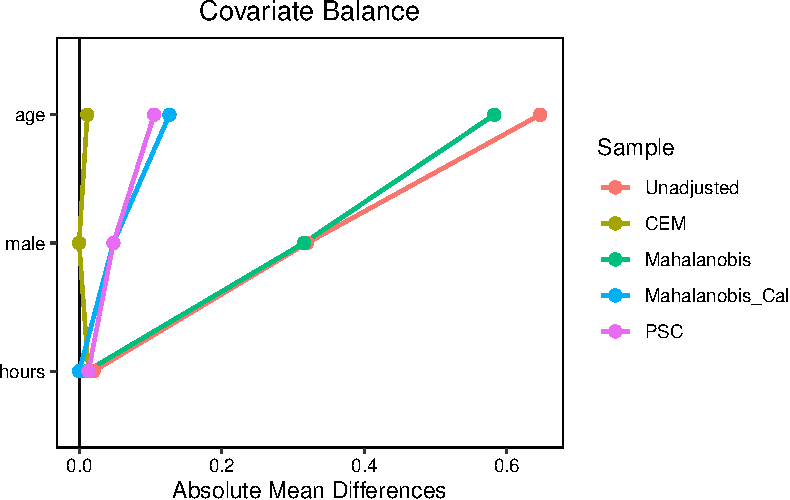
\includegraphics{Matching_files/figure-pdf/unnamed-chunk-37-1.pdf}

Die Grafik zeigt, dass Coarsened Exact Matching (CEM) unter allen
betrachteten Verfahren die Stichprobe mit der besten Balance ergibt.
Diesen gematchten Datensatz erhalten wir mit
\texttt{MatchIt::match.data()}.

\begin{Shaded}
\begin{Highlighting}[]
\CommentTok{\# gematchten Datensatz zuweisen}
\NormalTok{darkmode\_matched\_CEM }\OtherTok{\textless{}{-}} \FunctionTok{match.data}\NormalTok{(res\_CEM)}
\FunctionTok{head}\NormalTok{(darkmode\_matched\_CEM)}
\end{Highlighting}
\end{Shaded}

\begin{verbatim}
# A tibble: 6 x 7
  read_time dark_mode  male   age hours weights subclass
      <dbl>     <dbl> <dbl> <dbl> <dbl>   <dbl> <fct>   
1      15.4         0     1    55  125.       1 26      
2      20.9         1     0    23  643.       1 70      
3      21.5         1     0    29  190.       1 79      
4      22           1     0    18  334.       1 80      
5      17.4         0     0    53  279.       1 11      
6      20.4         0     0    43  138.       1 9       
\end{verbatim}

\texttt{darkmode\_matched} enthält Gewichte (\texttt{weights}) für die
jeweilige Gruppe zu denen gemachte Beobachtungen gehören
(\texttt{subclass}). Dies ist relevant, falls Beobachtungen mehrfach
gematcht werden. Wegen Eins-zu-eins-Matching \emph{ohne} Zurücklegen
gibt es in unserem Beispiel 82 Beobachtungspaare und sämtliche Gewichte
sind 1. Die Berücksichtigung der Gewicht in den nachfolgenden Aufrufen
von Schätzfunktionen (bspw.\texttt{lm()}) ist daher nicht nötig und
erfolgt lediglich zur Illustration der grundsätzlichen Vorgehensweise.

Eine Wiederholung der grafischen Analyse in Kapitel~\ref{sec-balance}
zeigt eine deutlich verbesserte Vergleichbarkeit hinsichtlich der
Verteilung der Matching-Variablen in \texttt{darkmode\_matched}.

\begin{Shaded}
\begin{Highlighting}[]
\NormalTok{darkmode\_matched\_CEM }\SpecialCharTok{\%\textgreater{}\%}
  \FunctionTok{group\_by}\NormalTok{(dark\_mode) }\SpecialCharTok{\%\textgreater{}\%}
  \FunctionTok{select}\NormalTok{(age, hours) }\SpecialCharTok{\%\textgreater{}\%}
  \FunctionTok{mutate\_all}\NormalTok{(scale) }\SpecialCharTok{\%\textgreater{}\%}
  \FunctionTok{pivot\_longer}\NormalTok{(}\AttributeTok{cols =} \FunctionTok{c}\NormalTok{(}\SpecialCharTok{{-}}\NormalTok{dark\_mode)) }\SpecialCharTok{\%\textgreater{}\%}
  
  \FunctionTok{ggplot}\NormalTok{(}
    \FunctionTok{aes}\NormalTok{(}\AttributeTok{x =}\NormalTok{ value, }\AttributeTok{fill =} \FunctionTok{as.factor}\NormalTok{(dark\_mode))}
\NormalTok{  ) }\SpecialCharTok{+}
  \FunctionTok{geom\_density}\NormalTok{( }\AttributeTok{alpha =}\NormalTok{ .}\DecValTok{5}\NormalTok{) }\SpecialCharTok{+} 
  \FunctionTok{facet\_wrap}\NormalTok{(}
    \AttributeTok{facets =} \SpecialCharTok{\textasciitilde{}}\NormalTok{ name, }
    \AttributeTok{scales =} \StringTok{"free"}\NormalTok{, }
    \AttributeTok{nrow =} \DecValTok{3}
\NormalTok{  )}
\end{Highlighting}
\end{Shaded}

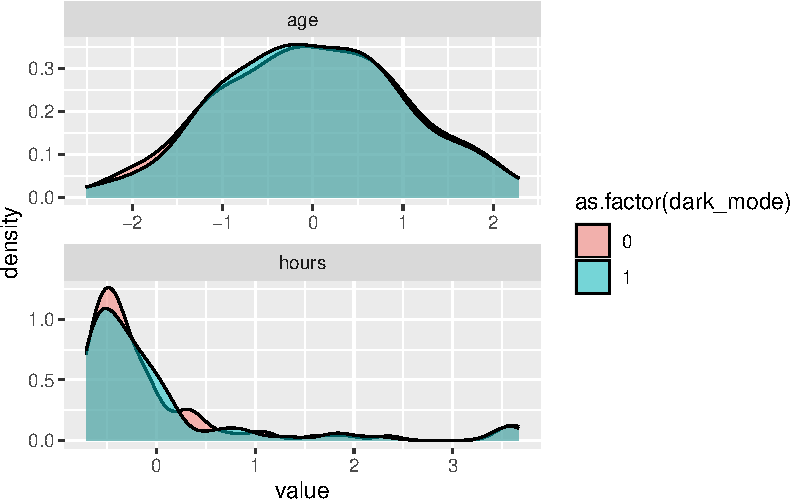
\includegraphics{Matching_files/figure-pdf/unnamed-chunk-39-1.pdf}

\begin{Shaded}
\begin{Highlighting}[]
\NormalTok{darkmode\_matched\_CEM }\SpecialCharTok{\%\textgreater{}\%} 
  \FunctionTok{group\_by}\NormalTok{(dark\_mode) }\SpecialCharTok{\%\textgreater{}\%}
  \FunctionTok{mutate}\NormalTok{(}
    \AttributeTok{male =} \FunctionTok{as.factor}\NormalTok{(male), }
    \AttributeTok{dark\_mode =} \FunctionTok{as.factor}\NormalTok{(dark\_mode)}
\NormalTok{  ) }\SpecialCharTok{\%\textgreater{}\%}
  
  \FunctionTok{ggplot}\NormalTok{(}
    \FunctionTok{aes}\NormalTok{(}\AttributeTok{x =}\NormalTok{ dark\_mode, }\AttributeTok{fill =}\NormalTok{ male)}
\NormalTok{  ) }\SpecialCharTok{+}
  \FunctionTok{geom\_bar}\NormalTok{(}\AttributeTok{position =} \StringTok{"fill"}\NormalTok{) }\SpecialCharTok{+}
  \FunctionTok{ylab}\NormalTok{(}\StringTok{"Anteil"}\NormalTok{)}
\end{Highlighting}
\end{Shaded}

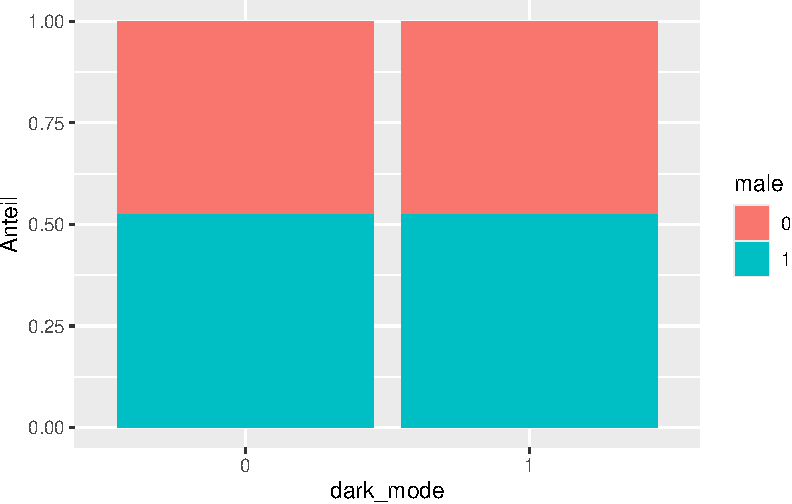
\includegraphics{Matching_files/figure-pdf/unnamed-chunk-39-2.pdf}

Wir beobachten eine bessere Balance bei \texttt{age} und \texttt{hours}.
Inbesondere ist \texttt{male} für Kontroll- und Behandlungsgruppe
ausgeglichen.

\section{Schätzung und Inferenz für den Behandlungseffekt nach
Matching}\label{sec-regadj}

Wir schätzen nun den Behandlungseffekt von \texttt{dark\_mode} auf
\texttt{read\_time} für die mit CEM und Propensity Score Matching
ermittelten Datensätzen und vergleichen die Ergebniss anschließend mit
einer Regressionsschätzung ohne Matching.

Wir kombinieren die Matching-Verfahren mit linearer Regression, d.h. wir
Schätzen den Behandlungseffekt anhand es gematchten Datensatzes als
Mittelwertdifferenz nach zusätzlicher Kontrolle für die
Matching-Variablen. Diese Kombination von Matching mit Regression wird
in der Literatur als \emph{Regression Adjustment} bezeichnet und ist
insbesondere hilfreich, wenn Backdoors mit Matching geschlossen werden
sollen, der kausale Effekt jedoch nur unter Verwendung einer
nicht-trivialen Regressionsfunktion ermittelt werden kann. Zum Beispiel
kann bei einer kontinuierlichen Behandlungsvariable und einem
nicht-linearen Zusammenhang mit \(Y\) der kausale Effekt nicht durch
einen bloßen Mittelwertvergleich erfasst werden, sondern erfordert eine
adäquate Modellierung dieses Zusammenhangs in der Regressionsfunktion.
Die zusätzliche Kontrolle für Matching-Variablen kann die Varianz der
Schätzung verringern und das Risiko einer verzerrten Schätzung
abmildern, falls nach Matching noch Unterschiede in der Balance von
Behandlungs- und Kontrollgruppe vorliegen.

\begin{Shaded}
\begin{Highlighting}[]
\CommentTok{\# ATT mit linearem Modell schätzen: CEM Datensatz}
\NormalTok{ATT\_mod\_CEM }\OtherTok{\textless{}{-}} \FunctionTok{lm}\NormalTok{(}
  \AttributeTok{formula =}\NormalTok{ read\_time }\SpecialCharTok{\textasciitilde{}}\NormalTok{ age }\SpecialCharTok{+}\NormalTok{ male }\SpecialCharTok{+}\NormalTok{ hours }\SpecialCharTok{+}\NormalTok{ dark\_mode,}
  \AttributeTok{data =}\NormalTok{ darkmode\_matched\_CEM, }
  \AttributeTok{weights =}\NormalTok{ weights }
\NormalTok{)}

\FunctionTok{summary}\NormalTok{(ATT\_mod\_CEM)}
\end{Highlighting}
\end{Shaded}

\begin{verbatim}

Call:
lm(formula = read_time ~ age + male + hours + dark_mode, data = darkmode_matched_CEM, 
    weights = weights)

Residuals:
    Min      1Q  Median      3Q     Max 
-8.9310 -2.3856 -0.0194  2.5407 14.0020 

Coefficients:
              Estimate Std. Error t value Pr(>|t|)    
(Intercept) 16.6088953  1.5255529  10.887  < 2e-16 ***
age          0.0380982  0.0344699   1.105  0.27072    
male        -4.0915725  0.6858131  -5.966 1.53e-08 ***
hours        0.0050129  0.0006977   7.185 2.45e-11 ***
dark_mode    1.6532234  0.6149439   2.688  0.00794 ** 
---
Signif. codes:  0 '***' 0.001 '**' 0.01 '*' 0.05 '.' 0.1 ' ' 1

Residual standard error: 3.937 on 159 degrees of freedom
Multiple R-squared:  0.414, Adjusted R-squared:  0.3992 
F-statistic: 28.08 on 4 and 159 DF,  p-value: < 2.2e-16
\end{verbatim}

\begin{Shaded}
\begin{Highlighting}[]
\CommentTok{\# Datensatz für Propensity Score Matching zuweisen}
\NormalTok{darkmode\_matched\_PSC }\OtherTok{\textless{}{-}} \FunctionTok{match.data}\NormalTok{(res\_PSC)}

\CommentTok{\# ATT mit linearem Modell schätzen: PSM Datensatz}
\NormalTok{ATT\_mod\_PSC }\OtherTok{\textless{}{-}} \FunctionTok{lm}\NormalTok{(}
  \AttributeTok{formula =}\NormalTok{ read\_time }\SpecialCharTok{\textasciitilde{}}\NormalTok{ age }\SpecialCharTok{+}\NormalTok{ male }\SpecialCharTok{+}\NormalTok{ hours }\SpecialCharTok{+}\NormalTok{ dark\_mode,}
  \AttributeTok{data =}\NormalTok{ darkmode\_matched\_PSC, }
  \AttributeTok{weights =}\NormalTok{ weights }
\NormalTok{)}

\FunctionTok{summary}\NormalTok{(ATT\_mod\_PSC)}
\end{Highlighting}
\end{Shaded}

\begin{verbatim}

Call:
lm(formula = read_time ~ age + male + hours + dark_mode, data = darkmode_matched_PSC, 
    weights = weights)

Residuals:
   Min     1Q Median     3Q    Max 
-9.972 -2.605 -0.044  2.587 14.951 

Coefficients:
              Estimate Std. Error t value Pr(>|t|)    
(Intercept) 17.3654519  1.2762648  13.606  < 2e-16 ***
age          0.0283941  0.0301484   0.942  0.34741    
male        -3.9858702  0.6480072  -6.151 4.03e-09 ***
hours        0.0046119  0.0006685   6.899 6.53e-11 ***
dark_mode    1.6346636  0.5769812   2.833  0.00507 ** 
---
Signif. codes:  0 '***' 0.001 '**' 0.01 '*' 0.05 '.' 0.1 ' ' 1

Residual standard error: 4.141 on 203 degrees of freedom
Multiple R-squared:  0.3171,    Adjusted R-squared:  0.3037 
F-statistic: 23.57 on 4 and 203 DF,  p-value: 5.098e-16
\end{verbatim}

\begin{Shaded}
\begin{Highlighting}[]
\CommentTok{\# ATT mit linearem Modell ohne Matching}
\NormalTok{ATT\_mod\_org }\OtherTok{\textless{}{-}} \FunctionTok{lm}\NormalTok{(}
  \AttributeTok{formula =}\NormalTok{ read\_time }\SpecialCharTok{\textasciitilde{}}\NormalTok{ age }\SpecialCharTok{+}\NormalTok{ male }\SpecialCharTok{+}\NormalTok{ hours }\SpecialCharTok{+}\NormalTok{ dark\_mode,}
  \AttributeTok{data =}\NormalTok{ darkmode}
\NormalTok{)}

\FunctionTok{summary}\NormalTok{(ATT\_mod\_org)}
\end{Highlighting}
\end{Shaded}

\begin{verbatim}

Call:
lm(formula = read_time ~ age + male + hours + dark_mode, data = darkmode)

Residuals:
     Min       1Q   Median       3Q      Max 
-10.2697  -2.6710   0.0164   2.5909  14.5739 

Coefficients:
             Estimate Std. Error t value Pr(>|t|)    
(Intercept) 16.859075   1.082303  15.577  < 2e-16 ***
age          0.051332   0.022215   2.311  0.02154 *  
male        -4.485545   0.498957  -8.990  < 2e-16 ***
hours        0.004348   0.000516   8.427 1.58e-15 ***
dark_mode    1.385810   0.523793   2.646  0.00859 ** 
---
Signif. codes:  0 '***' 0.001 '**' 0.01 '*' 0.05 '.' 0.1 ' ' 1

Residual standard error: 4.03 on 295 degrees of freedom
Multiple R-squared:  0.3434,    Adjusted R-squared:  0.3345 
F-statistic: 38.57 on 4 and 295 DF,  p-value: < 2.2e-16
\end{verbatim}

Beachte, dass für die gematchten Datensätze jeweils ein
durchschnittlicher Behandlungseffekt für die Beobachtungen \emph{mit}
erfolgter Behandlung ermittelt wird: In sämtlichen oben gezeigten
Matchibg-Verfahren werden mit \texttt{estimand\ =\ "ATT"}
vergleichbarere Kontrollbeobachtungen für die behandelten Beobachtungen
ermittelt. Wir schätzen den Effekt der Behandlung, indem wir die
Ergebnisse von behandelten Personen mit denen von gematchten Personen
vergleichen, die keine Behandlung erhalten haben. Diese Vergleichsgruppe
dient als Ersatz für den hypothetischen Zustand der Behandlungsgruppe,
wenn keine Behandlung erfolgt wäre. Dies entspricht der Definition eines
ATT --- ein average treatment effect \emph{on the treated}.

\subsection{Cluster-robuste
Standardfehler}\label{cluster-robuste-standardfehler}

Für Matching-Verfahren sind die mit \texttt{summary()} berechneten
Standardfehler (und damit auch Konfidenzintervalle, t-Statistiken und
p-Werte) für den Behandlungseffekt \emph{grundsätzlich ungültig}. Je
nach Matching-Verfahren liegen unterschiedliche Quellen von
Schätzunsicherheit vor, die bei der Berechnung von Standardfehlern
zusätzlich zu der ``üblichen'' Stichproben-Variabilität berücksichtig
werden müssen. Gründe hierfür sind der Matching-Prozess ansich oder
weitere Unsicherheit durch die Schätzung zusätzlicher Parameter, etwa
bei der Berechnung von Propensity Scores mit logistischer Regression.
Eine weiterere Ursache zusätzlicher Variation durch den
Matching-Prozess, die wir bisher nicht näher betrachtet haben ensteht
durch Zurücklegen, d.h. wenn Beobachtungen mehrfach gematcht werden
können. Auch dieser Faktor wird in der von \texttt{summary()}
verwendeten Formel für den Standardfehler des Effekt-Schätzers nicht
berücksichtigt.

Die Standardfehlerberechnung für Matching-Schätzer von
Behandlungseffekten ist ein Gegenstand aktueller methodischer Forschung.
P. C. Austin und Small (2014) und A. Abadie und Spiess (2022) belegen
die Gültigkeit von cluster-robusten Standardfehlern mit Clustering auf
Ebene der Beobachtungsgruppen (\texttt{subclass} im output von
\texttt{match.data()}) bei Matching ohne Zurücklegen. Für Matching
anhand von Propensity Scores (auch mit Zurücklegen) zeigt Imbens (2016),
dass ignorieren der zusätzlichen Unsicherheit durch die Schätzung der
Propensity Scores zu konservativer Inferenz für den ATE anhand eines
cluster-robusten Standardfehlerschätzers führt, jedoch ungültige
Inferenz für die Schätzung des ATT bedeuten kann. Ähnlich zu P. C.
Austin und Small (2014) deuten die Ergebnisse der Simulationsstudie von
Bodory u.~a. (2020) jedoch auf grundsätzlich bessere Eigenschaften der
Schätzung hin, wenn die Standardfehler \emph{nicht} für die Schätzung
der Propensity Scores adjustiert werden.

Weiterhin ist die Kontrolle für Kovariablen mit Erklärungskraft für die
Outcome-Variable und für die Matching-Variablen mit \emph{Regression
Adjustment} (vgl. Kapitel~\ref{sec-regadj}) für die Schätzung des
Behandlungseffekts nach Matching eine etablierte Strategie, vgl. Hill
und Reiter (2006) und A. Abadie und Spiess (2022). So können die Varianz
der Schätzung und das Risiko einer Verzerrung der Standardfehler
aufgrund verbleibender Imbalance von Behandlungs- und Kontrollgruppe
nach Matching verringert werden.

Zur Demonstration von (cluster)-robuster Inferenz und für eine
tabellarische Zusammenfassung der Ergebnisse nutzen wir die Pakete
\texttt{marginaleffects} und \texttt{modelsummary}. Mit
\texttt{marginaleffects::avg\_comparisons()} können p-Werte und
Kofindenzintervalle unter Berücksichtigung von robuster Standardfehlern
und der Gewichte aus dem Matching-Verfahren berechnet werden.

\begin{Shaded}
\begin{Highlighting}[]
\FunctionTok{library}\NormalTok{(marginaleffects)}

\CommentTok{\# Inferenz: Multiple Regression, ungematchter Datensatz}
\NormalTok{(}
\NormalTok{  sum\_orig }\OtherTok{\textless{}{-}} \FunctionTok{avg\_comparisons}\NormalTok{(}
    \AttributeTok{model =}\NormalTok{ ATT\_mod\_org,}
    \AttributeTok{variables =} \StringTok{"dark\_mode"}\NormalTok{,}
    \CommentTok{\# Heteroskedastie{-}robuste SE:}
    \AttributeTok{vcov =} \StringTok{"HC3"}\NormalTok{, }
    \CommentTok{\# Identifizierung der Kontrollgruppe:}
    \AttributeTok{newdata =} \FunctionTok{subset}\NormalTok{(darkmode, dark\_mode }\SpecialCharTok{==} \DecValTok{1}\NormalTok{) }
\NormalTok{  )}
\NormalTok{) }
\end{Highlighting}
\end{Shaded}

\begin{verbatim}

      Term          Contrast Estimate Std. Error    z Pr(>|z|)   S 2.5 % 97.5 %
 dark_mode mean(1) - mean(0)     1.39      0.537 2.58  0.00988 6.7 0.333   2.44

Columns: term, contrast, estimate, std.error, statistic, p.value, s.value, conf.low, conf.high, predicted_lo, predicted_hi, predicted 
Type:  response 
\end{verbatim}

\begin{Shaded}
\begin{Highlighting}[]
\CommentTok{\# Inferenz: Multiple Regression bei CEM}
\NormalTok{(}
\NormalTok{  sum\_CEM }\OtherTok{\textless{}{-}} \FunctionTok{avg\_comparisons}\NormalTok{(}
  \AttributeTok{model =}\NormalTok{ ATT\_mod\_CEM ,}
  \AttributeTok{variables =} \StringTok{"dark\_mode"}\NormalTok{,}
  \CommentTok{\# Cluster{-}robuste SE}
  \AttributeTok{vcov =} \SpecialCharTok{\textasciitilde{}}\NormalTok{ subclass, }
  \AttributeTok{newdata =} \FunctionTok{subset}\NormalTok{(darkmode\_matched\_CEM, dark\_mode }\SpecialCharTok{==} \DecValTok{1}\NormalTok{),}
  \AttributeTok{wts =} \StringTok{"weights"}
\NormalTok{  )}
\NormalTok{)}
\end{Highlighting}
\end{Shaded}

\begin{verbatim}

      Term          Contrast Estimate Std. Error    z Pr(>|z|)   S 2.5 % 97.5 %
 dark_mode mean(1) - mean(0)     1.65      0.549 3.01  0.00262 8.6 0.576   2.73

Columns: term, contrast, estimate, std.error, statistic, p.value, s.value, conf.low, conf.high, predicted_lo, predicted_hi, predicted 
Type:  response 
\end{verbatim}

\begin{Shaded}
\begin{Highlighting}[]
\CommentTok{\# Inferenz: Multiple Regression bei PSM}
\NormalTok{(}
\NormalTok{  sum\_PSC }\OtherTok{\textless{}{-}} \FunctionTok{avg\_comparisons}\NormalTok{(}
    \AttributeTok{model =}\NormalTok{ ATT\_mod\_PSC ,}
    \AttributeTok{variables =} \StringTok{"dark\_mode"}\NormalTok{,}
    \AttributeTok{vcov =} \SpecialCharTok{\textasciitilde{}}\NormalTok{ subclass, }
    \AttributeTok{newdata =} \FunctionTok{subset}\NormalTok{(darkmode\_matched\_PSC, dark\_mode }\SpecialCharTok{==} \DecValTok{1}\NormalTok{),}
    \AttributeTok{wts =} \StringTok{"weights"}
\NormalTok{  )}
\NormalTok{)}
\end{Highlighting}
\end{Shaded}

\begin{verbatim}

      Term          Contrast Estimate Std. Error    z Pr(>|z|)   S 2.5 % 97.5 %
 dark_mode mean(1) - mean(0)     1.63      0.565 2.89  0.00381 8.0 0.527   2.74

Columns: term, contrast, estimate, std.error, statistic, p.value, s.value, conf.low, conf.high, predicted_lo, predicted_hi, predicted 
Type:  response 
\end{verbatim}

Wir fassen die Ergebnisse mit \texttt{modelsummary::modelsummary()}
tabellarisch zusammen.

\begin{Shaded}
\begin{Highlighting}[]
\FunctionTok{library}\NormalTok{(modelsummary)}

\CommentTok{\# Tabellarische Zusammenfassung erzeugen}
\FunctionTok{modelsummary}\NormalTok{(}
  \AttributeTok{models =} \FunctionTok{list}\NormalTok{(}
   \StringTok{"Kein Matching"} \OtherTok{=}\NormalTok{ sum\_orig, }
   \StringTok{"Coarsened Exact"} \OtherTok{=}\NormalTok{ sum\_CEM, }
   \StringTok{"Propensity Scores"} \OtherTok{=}\NormalTok{ sum\_PSC}
\NormalTok{  ),}
  \AttributeTok{stars =}\NormalTok{ T, }
  \AttributeTok{gof\_map =} \StringTok{"nobs"}\NormalTok{, }
  \AttributeTok{output =} \StringTok{"gt"}
\NormalTok{) }\SpecialCharTok{\%\textgreater{}\%}
  \FunctionTok{tabopts}\NormalTok{()}
\end{Highlighting}
\end{Shaded}

\setlength{\LTpost}{0mm}
\begin{longtable*}{lccc}
\toprule
  & Kein Matching & Coarsened Exact & Propensity Scores \\ 
\midrule\addlinespace[2.5pt]
dark\_mode & 1.386** & 1.653** & 1.635** \\ 
 & (0.537) & (0.549) & (0.565) \\ 
Num.Obs. & 300 & 164 & 208 \\ 
\bottomrule
\end{longtable*}
\begin{minipage}{\linewidth}
+ p < 0.1, * p < 0.05, ** p < 0.01, *** p < 0.001\\
\end{minipage}

\section{Bootstrap-Schätzung kausaler Effekte bei
Matching}\label{sec-bootmatching}

Ein Bootstrap-Verfahren generiert mit Resampling (wiederholtes Ziehen
mit Zurücklegen) aus dem Original-Datensatz (viele) künstliche
Datensätze, für die der Schätzer (d.h. das gesamte Verfahren inkl.
Matching!) jeweils berechnet wird. Die Verteilung der so gewonnenen
Bootstrap-Schätzwerte approximiert die wahre, unbekannte
Stichprobenverteilung des Schätzers des Behandlungseffekts. Mit dieser
simulierten Verteilung können wir Inferenz betreiben: Wir können einen
Bootstrap-Punktschätzer des Behandlungseffekts (Stichprobenmittel der
Bootstrap-Schätzungen) sowie Standardfehler (Standardabweichung der der
Bootstrap-Schätzungen) und p-Werte berechnen.

Der Bootstrap kann hilfreich sein, wenn unklar ist, wie Standardfehler
für die Unsicherheit des Matching-Prozesses zu adjustieren sind, um
gültige Inferenzsstatistiken zu erhalten. A. Abadie und Imbens (2008)
zeigen analytisch, dass der Standard-Bootstrap die Stichprobenverteilung
für Schätzer kausaler Effekte anhand von gematchten Datensätzen (d.h.
bei Zuordnung/Selektion von Beobachtungen mit Matching) nicht korrekt
abbilden kann. Grundsätzlich problematisch hierbei ist, wenn der
Bootstrap eine verzerrte Schätzung produziert und/oder zu kleine
Standardfehler liefert. A. Abadie und Imbens (2008) belegen die Tendenz
des Bootstraps zu \emph{konservative} (d.h. zu große) Standardfehler zu
produzieren. Simulationsnachweise (Bodory u.~a. 2020; Hill und Reiter
2006; P. C. Austin und Small 2014; P. C. Austin und Stuart 2017) finden,
dass Bootstrap-Standardfehler u.a. bei Propensity Score Matching mit
Zurücklegen leicht konservativ sind somit das gewünschte nominale
Signifikanzniveau eines Bootstrap-Hypothesentests nicht überschritten
wird, weshalb der Standard-Bootstrap trotz seiner Schwächen in der
empirischen Forschung oft angewendet wird.

Wir betrachen als nächstes einen Bootstrap-Algorithmus für Inferenz
bezüglich eines kausalen Effekts nach Matching und demonstrieren die
Schätzung anhand unseres Website-Beispiels für den ATT nach
Propensity-Score-Matching.

\begin{tcolorbox}[enhanced jigsaw, bottomtitle=1mm, colbacktitle=quarto-callout-tip-color!10!white, coltitle=black, arc=.35mm, title={\textbf{Algorithmus: Bootstrap-Schätzer für Matching mit Regression
Adjustment}}, titlerule=0mm, opacityback=0, breakable, bottomrule=.15mm, toprule=.15mm, opacitybacktitle=0.6, colframe=quarto-callout-tip-color-frame, toptitle=1mm, rightrule=.15mm, leftrule=.75mm, left=2mm, colback=white]

\begin{enumerate}
\def\labelenumi{\arabic{enumi}.}
\item
  Generiere eine Bootstrap-Stichprobe durch \(N\) Züge \emph{mit
  Zurücklegen} aus der \(N\)-elementigen originalen Stichprobe.
\item
  Wende das Matching-Verfahren für die Bootstrap-Stichprobe an. Schätze
  den Behandlungseffekt \(\beta\) anhand der gematchten Stichprobe mit
  Regression. Speichere den Punktschätzer des Behandlungseffekts
  \(\widehat{\beta}_b^*\).
\item
  Fürhre die Schritte 1 und 2 für \(b=1,\dots,B\) aus, wobei \(B\) eine
  hinreichend große Anzahl von Bootstrap-Replikationen ist.
\item
  Berechne den Bootstrap-Schätzer des Behandlungseffekts
  \(\overline{\beta}^* = \frac{1}{B}\sum_{b=1} \widehat{\beta}_b^*\) und
  den Standardfehler
  \(\text{SE}(\overline{\beta}^*) = \sqrt{\frac{1}{B-1}\sum_{b=1}^B(\widehat{\beta}_b^*-\overline{\beta}^*)^2}\).
  Berechne Inferenz-Statistiken mit den üblichen Formeln.
\end{enumerate}

\end{tcolorbox}

Wir Implementieren nun einen Bootstrap-Schätzer des ATT im
Website-Beispiel für Propensity-Score-Matching. Hierzu definieren wir
eine \texttt{R}-Funktion \texttt{boot\_fun()} für die Schritte 1 und 2
im obigen Algorithmus.

\begin{Shaded}
\begin{Highlighting}[]
\CommentTok{\# Bootstrap{-}Funktion für Schritte 1 und 2}
\NormalTok{boot\_fun }\OtherTok{\textless{}{-}} \ControlFlowTok{function}\NormalTok{(}
\NormalTok{    data, }\CommentTok{\# originale Stichprobe}
\NormalTok{    i     }\CommentTok{\# Indexmenge f. Bootstrap{-}Stichprobe}
\NormalTok{) \{}
  
  \CommentTok{\# Bootstrap{-}Stichprobe}
\NormalTok{  boot\_data }\OtherTok{\textless{}{-}}\NormalTok{ data[i, ]}
  
  \CommentTok{\# 1:1 PS Matching}
\NormalTok{  match\_res }\OtherTok{\textless{}{-}} \FunctionTok{matchit}\NormalTok{(}
\NormalTok{    dark\_mode }\SpecialCharTok{\textasciitilde{}}\NormalTok{ age }\SpecialCharTok{+}\NormalTok{ hours }\SpecialCharTok{+}\NormalTok{ male,}
    \AttributeTok{estimand =} \StringTok{"ATT"}\NormalTok{,}
    \AttributeTok{distance =} \StringTok{"glm"}\NormalTok{, }
    \AttributeTok{method =} \StringTok{"nearest"}\NormalTok{, }
    \AttributeTok{caliper =}\NormalTok{ .}\DecValTok{25}\NormalTok{,}
    \AttributeTok{data =}\NormalTok{ boot\_data}
\NormalTok{  ) }
  
  \CommentTok{\# Gematchten Datensatz zuweisen}
\NormalTok{  darkmode\_matched }\OtherTok{\textless{}{-}} \FunctionTok{match.data}\NormalTok{(}
    \AttributeTok{object =}\NormalTok{ match\_res, }
    \AttributeTok{data =}\NormalTok{ boot\_data}
\NormalTok{  )}
  
  \CommentTok{\# Outcome{-}Modell schätzen}
\NormalTok{  ATT\_mod }\OtherTok{\textless{}{-}} \FunctionTok{lm}\NormalTok{(}
    \AttributeTok{formula =}\NormalTok{ read\_time }\SpecialCharTok{\textasciitilde{}}\NormalTok{ age }\SpecialCharTok{+}\NormalTok{ male }\SpecialCharTok{+}\NormalTok{ hours }\SpecialCharTok{+}\NormalTok{ dark\_mode,}
    \AttributeTok{data =}\NormalTok{ darkmode\_matched, }
    \AttributeTok{weights =}\NormalTok{ weights }
\NormalTok{  )}
  
  \CommentTok{\#  ATT{-}Schätzung zurückgeben}
  \FunctionTok{return}\NormalTok{(}
\NormalTok{    ATT\_mod}\SpecialCharTok{$}\NormalTok{coefficients[}\StringTok{"dark\_mode"}\NormalTok{]  }
\NormalTok{  )}
\NormalTok{\}}
\end{Highlighting}
\end{Shaded}

Wir berechnen nun eine Bootstrap-Schätzung des ATT von
\texttt{dark\_mode} auf \texttt{readingtime} nach Propensity Score
Matching mit einem caliper von 0.25 sowie den zugehörigen Standardfehler
und ein 95\%-KI mit der zuvor definierten Funktion \texttt{boot\_fun}.

\begin{Shaded}
\begin{Highlighting}[]
\FunctionTok{library}\NormalTok{(}\StringTok{"boot"}\NormalTok{)}
\FunctionTok{set.seed}\NormalTok{(}\DecValTok{4321}\NormalTok{)}

\CommentTok{\# Anz. Bootstrap{-}Replikationen}
\NormalTok{B }\OtherTok{\textless{}{-}} \DecValTok{999}

\CommentTok{\# Bootstrap durchführen}
\NormalTok{(}
\NormalTok{  boot\_out }\OtherTok{\textless{}{-}} \FunctionTok{boot}\NormalTok{(darkmode, boot\_fun, }\AttributeTok{R =}\NormalTok{ B)}
\NormalTok{)}
\end{Highlighting}
\end{Shaded}

\begin{verbatim}

ORDINARY NONPARAMETRIC BOOTSTRAP


Call:
boot(data = darkmode, statistic = boot_fun, R = B)


Bootstrap Statistics :
    original      bias    std. error
t1* 1.634664 -0.08144129   0.5935746
\end{verbatim}

Den Bootstrap-Schätzer des ATT sowie den Bootstrap-Standardfehler
berechnen wir mit \texttt{mean()} und \texttt{sd()} anhand der 999
Bootstrap-Replikationen in \texttt{boot\_out\$t}.

Beachte, dass der Bootstrap-Schätzer des Behandlungseffekts nicht
unmittelbar von \texttt{boot()} ausgegeben wird. \texttt{original} ist
die Schätzung anhand der gesamten Stichprobe (d.h. ohne Bootstrap) und
\texttt{bias} ist die Differenz zwischen dieser Schätzung und dem
Mittelwert der Bootstrap-Schätzungen.

\begin{Shaded}
\begin{Highlighting}[]
\CommentTok{\# Bootstrap{-}Schätzer für den Treatment{-}Effekt}
\FunctionTok{mean}\NormalTok{(boot\_out}\SpecialCharTok{$}\NormalTok{t) }
\end{Highlighting}
\end{Shaded}

\begin{verbatim}
[1] 1.553222
\end{verbatim}

\begin{Shaded}
\begin{Highlighting}[]
\CommentTok{\# bootstrap {-} original = bias}
\FunctionTok{mean}\NormalTok{(boot\_out}\SpecialCharTok{$}\NormalTok{t) }\SpecialCharTok{{-}}\NormalTok{ boot\_out}\SpecialCharTok{$}\NormalTok{t0}
\end{Highlighting}
\end{Shaded}

\begin{verbatim}
  dark_mode 
-0.08144129 
\end{verbatim}

Wir können prüfen, dass die Berechnung des Standardfehlers dem
Stichprobenstandardabweichung der Bootstrap-Schätzungen entspricht.

\begin{Shaded}
\begin{Highlighting}[]
\CommentTok{\# Bootstrap{-}Standardfehler}
\FunctionTok{sd}\NormalTok{(boot\_out}\SpecialCharTok{$}\NormalTok{t)}
\end{Highlighting}
\end{Shaded}

\begin{verbatim}
[1] 0.5935746
\end{verbatim}

Ein 95\%-Konfidenzintervall für den kausalen Effekt erhalten wir mit
\texttt{boot::boot.ci()}.\footnote{\texttt{type\ =\ "bca"}
  (bias-corrected accelerated) ist eine gängige Implementierung für die
  Berechnung des Konfidenz-Intervalls.}

\begin{Shaded}
\begin{Highlighting}[]
\CommentTok{\# 95\% Bootstrap{-}KI für den Treatment{-}Effekt}
\FunctionTok{boot.ci}\NormalTok{(}
  \AttributeTok{boot.out =}\NormalTok{ boot\_out, }
  \AttributeTok{type =} \StringTok{"bca"}\NormalTok{, }
  \AttributeTok{conf =}\NormalTok{ .}\DecValTok{95}
\NormalTok{)}
\end{Highlighting}
\end{Shaded}

\begin{verbatim}
BOOTSTRAP CONFIDENCE INTERVAL CALCULATIONS
Based on 999 bootstrap replicates

CALL : 
boot.ci(boot.out = boot_out, conf = 0.95, type = "bca")

Intervals : 
Level       BCa          
95%   ( 0.527,  2.839 )  
Calculations and Intervals on Original Scale
\end{verbatim}

Beachte, dass der Bootstrap-Standardfehler sowie das
Bootstrap-Konfidenzintervall nahe der mit \texttt{avg\_comarisons}
berechneten Werte für \texttt{sum\_PSC} sind.

\textbf{Bootstrap-Standardfehler für IPW-Schätzer des ATE berechnen}

Die Bootstrap-Funktion \texttt{boot\_fun} kann leicht für eine Schätzung
des Standardfehlers für den IPW-Schätzer des ATE aus
Kapitel~\ref{sec-PSM} angepasst werden. Statt einer Matching-Prozedur
berechnen wir hierzu für \(B\) Bootstrap-Stichproben den Schätzer
\(\widehat{\tau}^\text{IPW}\) mit Trimming der Propensity Scores.

\begin{Shaded}
\begin{Highlighting}[]
\CommentTok{\# IPW estimation with regression adjustment}
\NormalTok{IPW\_boot }\OtherTok{\textless{}{-}} \ControlFlowTok{function}\NormalTok{(}
\NormalTok{    data, }
\NormalTok{    i}
\NormalTok{) \{}
  
  \CommentTok{\# Bootstrap{-}Stichprobe erstellen}
\NormalTok{  data\_boot  }\OtherTok{\textless{}{-}}\NormalTok{ data }\SpecialCharTok{\%\textgreater{}\%} 
    \FunctionTok{slice}\NormalTok{(i)}
  
  \CommentTok{\# Logistischee Regression}
\NormalTok{  glm\_fit }\OtherTok{\textless{}{-}} \FunctionTok{glm}\NormalTok{(}
    \AttributeTok{formula =}\NormalTok{ dark\_mode }\SpecialCharTok{\textasciitilde{}}\NormalTok{ age }\SpecialCharTok{+}\NormalTok{ hours }\SpecialCharTok{+}\NormalTok{ male,}
    \AttributeTok{data =}\NormalTok{ data\_boot, }
    \AttributeTok{family =}\NormalTok{ binomial}
\NormalTok{  )}
  
  \CommentTok{\# Propensity Scores berechnen}
\NormalTok{  data\_boot }\OtherTok{\textless{}{-}}\NormalTok{ data\_boot }\SpecialCharTok{\%\textgreater{}\%}
    \FunctionTok{mutate}\NormalTok{(}
      \AttributeTok{ps =} \FunctionTok{predict}\NormalTok{(glm\_fit, }\AttributeTok{type =} \StringTok{\textquotesingle{}response\textquotesingle{}}\NormalTok{)}
\NormalTok{    )}
  
  \CommentTok{\# Beobachtungen anhand Propensity Scores trimmen}
\NormalTok{  data\_boot }\OtherTok{\textless{}{-}}\NormalTok{ data\_boot }\SpecialCharTok{\%\textgreater{}\%}
    \FunctionTok{filter}\NormalTok{(}
      \FunctionTok{between}\NormalTok{(}
        \AttributeTok{x =}\NormalTok{ ps,}
        \AttributeTok{left =}\NormalTok{ .}\DecValTok{2}\NormalTok{,}
        \AttributeTok{right =}\NormalTok{ .}\DecValTok{7}
\NormalTok{      )}
\NormalTok{    )}
  
  \CommentTok{\# IPW berechnen}
\NormalTok{  data\_boot }\OtherTok{\textless{}{-}}\NormalTok{ data\_boot }\SpecialCharTok{\%\textgreater{}\%}
    \FunctionTok{mutate}\NormalTok{(}
      \AttributeTok{ipw =} \FunctionTok{case\_when}\NormalTok{(}
\NormalTok{        dark\_mode }\SpecialCharTok{==} \DecValTok{1} \SpecialCharTok{\textasciitilde{}} \DecValTok{1} \SpecialCharTok{/}\NormalTok{ ps,}
\NormalTok{        dark\_mode }\SpecialCharTok{==} \DecValTok{0} \SpecialCharTok{\textasciitilde{}} \DecValTok{1} \SpecialCharTok{/}\NormalTok{ (}\DecValTok{1} \SpecialCharTok{{-}}\NormalTok{ ps))}
\NormalTok{    )}
  
  \CommentTok{\# Gewichtete Mittelwerte der Gruppen   }
\NormalTok{  w\_means }\OtherTok{\textless{}{-}}\NormalTok{ data\_boot }\SpecialCharTok{\%\textgreater{}\%}
    \FunctionTok{group\_by}\NormalTok{(dark\_mode) }\SpecialCharTok{\%\textgreater{}\%}
    \FunctionTok{summarize}\NormalTok{(}\AttributeTok{m =} \FunctionTok{weighted.mean}\NormalTok{(read\_time, }\AttributeTok{w =}\NormalTok{ ipw)) }\SpecialCharTok{\%\textgreater{}\%}
    \FunctionTok{arrange}\NormalTok{(dark\_mode)}
  
  \CommentTok{\# ATT{-}Schätzwert}
  \FunctionTok{return}\NormalTok{(w\_means}\SpecialCharTok{$}\NormalTok{m[}\DecValTok{2}\NormalTok{] }\SpecialCharTok{{-}}\NormalTok{ w\_means}\SpecialCharTok{$}\NormalTok{m[}\DecValTok{1}\NormalTok{])}
\NormalTok{\}}
\end{Highlighting}
\end{Shaded}

\begin{Shaded}
\begin{Highlighting}[]
\FunctionTok{set.seed}\NormalTok{(}\DecValTok{1234}\NormalTok{)}
\CommentTok{\# Bootstrap für IPW durchführen}
\NormalTok{(}
\NormalTok{  b\_IPW }\OtherTok{\textless{}{-}} \FunctionTok{boot}\NormalTok{(}
    \AttributeTok{data =}\NormalTok{ darkmode,}
    \AttributeTok{statistic =}\NormalTok{ IPW\_boot, }
    \AttributeTok{R =} \DecValTok{999}
\NormalTok{  )}
\NormalTok{)}
\end{Highlighting}
\end{Shaded}

\begin{verbatim}

ORDINARY NONPARAMETRIC BOOTSTRAP


Call:
boot(data = darkmode, statistic = IPW_boot, R = 999)


Bootstrap Statistics :
    original     bias    std. error
t1* 1.962849 0.06297654   0.6599891
\end{verbatim}

\begin{Shaded}
\begin{Highlighting}[]
\CommentTok{\# Bootstrap{-}Schätzer und Standardfehler berechnen}
\FunctionTok{mean}\NormalTok{(b\_IPW}\SpecialCharTok{$}\NormalTok{t)}
\end{Highlighting}
\end{Shaded}

\begin{verbatim}
[1] 2.025826
\end{verbatim}

\begin{Shaded}
\begin{Highlighting}[]
\FunctionTok{sd}\NormalTok{(b\_IPW}\SpecialCharTok{$}\NormalTok{t)}
\end{Highlighting}
\end{Shaded}

\begin{verbatim}
[1] 0.6599891
\end{verbatim}

In diesem Fall ist der Bootstrap-Standardfehler von ca. 0.66 gut mit dem
anhand von \texttt{summary(model\_ipw)} berechneten Standardfehler
vergleichbar. Ein 95\%-Konfidenzintervall für den ATE erhalten wir wie
zuvor mit \texttt{boot.ci()}.

\begin{Shaded}
\begin{Highlighting}[]
\CommentTok{\# 95\% Bootstrap{-}KI für den ATE}
\FunctionTok{boot.ci}\NormalTok{(b\_IPW, }\AttributeTok{type =} \StringTok{"bca"}\NormalTok{)}
\end{Highlighting}
\end{Shaded}

\begin{verbatim}
BOOTSTRAP CONFIDENCE INTERVAL CALCULATIONS
Based on 999 bootstrap replicates

CALL : 
boot.ci(boot.out = b_IPW, type = "bca")

Intervals : 
Level       BCa          
95%   ( 0.563,  3.134 )  
Calculations and Intervals on Original Scale
\end{verbatim}

\section{Regression, Matching und
Doubly-Robust-Schätzung}\label{regression-matching-und-doubly-robust-schuxe4tzung}

Als \emph{Doubly-Robust-Schätzer} bezeichnet man Methoden, die bei
Fehlspezifikationen im Matching-Verfahrens \emph{oder} der funktionalen
Form der Regressionsfunktion für die Outcome-Variable eine zuverlässige
Schätzungen des kausalen Effekts ermöglichen.\footnote{Bspw. kann eine
  falsche funktionale Form bei logistischer Regression eine verzerrte
  Schätzung von Propensity Scores und damit eine unzureichende Balance
  bedeuten.} Unter der Vorraussetzung, dass die verwendeten
Matching-Variablen sämliche Backdoors schließen, ist so mit
Doubly-Robust-Schätzung eine konsistente Schätzung des
Behandlungseffekts unter abgeschwächten Annahmen gewähtleistet. Dies
macht Doubly-Robust-Schätzer besonders nützlich in Forschungskontexten,
in denen präzise Modellspezifikationen herausfordernd sind.

Der von Wooldridge (2010) vorgeschlagene Doubly-Robust-Schätzer (IPWRA)
für den ATE erreicht seine vorteilhaften Eigenschaften durch eine
geschickte Kombination von IPW und Regression Adjustment.

\begin{tcolorbox}[enhanced jigsaw, bottomtitle=1mm, colbacktitle=quarto-callout-tip-color!10!white, coltitle=black, arc=.35mm, title={\textbf{Algorithmus: IPWRA-Schätzer des ATE}}, titlerule=0mm, opacityback=0, breakable, bottomrule=.15mm, toprule=.15mm, opacitybacktitle=0.6, colframe=quarto-callout-tip-color-frame, toptitle=1mm, rightrule=.15mm, leftrule=.75mm, left=2mm, colback=white]

Vgl. Wooldridge (2010).

\begin{enumerate}
\def\labelenumi{\arabic{enumi}.}
\item
  Berechne IPW anhand von Propensity Score mit logistischer Regression
  unter Verwendung der Matching-Variablen.
\item
  Regression Adjustment:

  \begin{enumerate}
  \def\labelenumii{(\alph{enumii})}
  \item
    Schätze lediglich für die \emph{Behandlungsgruppe} eine mit den IPW
    gewichtete Regressionspezifikation der Outcome-Variable mit
    Kontrolle für die Matching-Variablen.
  \item
    Wiederhole Schritt A für \emph{Kontrollgruppe}.
  \end{enumerate}
\item
  Berechne Vorhersagen der Outcome-Variable für die angepassten Modelle
  aus 2 (a) und 2 (b) anhand des \emph{gesamten} Datensatzes.
\item
  Schätze den ATE als Mittelwert-Differenz der Vorhersagen aus Schritt
  3.
\end{enumerate}

\end{tcolorbox}

Wir implementieren den Doubly-Robust-Schätzer des ATE von Wooldridge
(2010) für das Website-Beispiel in der Funktion \texttt{IPWRA()} under
Adaption des Schemas von \texttt{IPW\_boot()}.

\begin{Shaded}
\begin{Highlighting}[]
\CommentTok{\# IPW estimation with regression adjustment}
\NormalTok{IPWRA }\OtherTok{\textless{}{-}} \ControlFlowTok{function}\NormalTok{(}
\NormalTok{    data, }
    \AttributeTok{i =}\NormalTok{ i) \{}
  
    \CommentTok{\# Bootstrap{-}Stichprobe zuweisen}
\NormalTok{    b\_data }\OtherTok{\textless{}{-}}\NormalTok{ data }\SpecialCharTok{\%\textgreater{}\%} 
      \FunctionTok{slice}\NormalTok{(i)}
    
    \CommentTok{\# Logistische Regression}
\NormalTok{    glm\_fit }\OtherTok{\textless{}{-}} \FunctionTok{glm}\NormalTok{(}
      \AttributeTok{formula =}\NormalTok{ dark\_mode }\SpecialCharTok{\textasciitilde{}}\NormalTok{ age }\SpecialCharTok{+}\NormalTok{ hours }\SpecialCharTok{+}\NormalTok{ male,}
      \AttributeTok{data =}\NormalTok{ b\_data, }
      \AttributeTok{family =} \FunctionTok{binomial}\NormalTok{(}\AttributeTok{link =} \StringTok{\textquotesingle{}logit\textquotesingle{}}\NormalTok{)}
\NormalTok{    )}
    
    \CommentTok{\# Propensity Scores berechnen}
\NormalTok{    b\_data }\OtherTok{\textless{}{-}}\NormalTok{ b\_data }\SpecialCharTok{\%\textgreater{}\%}
        \FunctionTok{mutate}\NormalTok{(}\AttributeTok{ps =} \FunctionTok{predict}\NormalTok{(glm\_fit, }\AttributeTok{type =} \StringTok{\textquotesingle{}response\textquotesingle{}}\NormalTok{))}
    
    \CommentTok{\# Propensity Scores trimmen}
\NormalTok{    b\_data }\OtherTok{\textless{}{-}}\NormalTok{ b\_data }\SpecialCharTok{\%\textgreater{}\%}
      \FunctionTok{filter}\NormalTok{(}
        \FunctionTok{between}\NormalTok{(}
          \AttributeTok{x =}\NormalTok{ ps,}
          \AttributeTok{left =}\NormalTok{ .}\DecValTok{2}\NormalTok{,}
          \AttributeTok{right =}\NormalTok{ .}\DecValTok{7}
\NormalTok{          )}
\NormalTok{    )}
    
    \CommentTok{\# IPW berechnen}
\NormalTok{    b\_data }\OtherTok{\textless{}{-}}\NormalTok{ b\_data }\SpecialCharTok{\%\textgreater{}\%}
      \FunctionTok{mutate}\NormalTok{(}
        \AttributeTok{IPW =} \FunctionTok{case\_when}\NormalTok{(}
\NormalTok{          dark\_mode }\SpecialCharTok{==} \DecValTok{1} \SpecialCharTok{\textasciitilde{}} \DecValTok{1} \SpecialCharTok{/}\NormalTok{ ps,}
\NormalTok{          dark\_mode }\SpecialCharTok{==} \DecValTok{0} \SpecialCharTok{\textasciitilde{}} \DecValTok{1} \SpecialCharTok{/}\NormalTok{ (}\DecValTok{1} \SpecialCharTok{{-}}\NormalTok{ ps))}
\NormalTok{      )}
    
    \CommentTok{\# Regression Adjustment:}
    
    \CommentTok{\# Schätzung des Behandlungseffekts für die ges. Stichprobe}
    \CommentTok{\# mit Modell für Behandlungsgruppe}
\NormalTok{    mtreat }\OtherTok{\textless{}{-}}\NormalTok{ b\_data }\SpecialCharTok{\%\textgreater{}\%}
      \FunctionTok{filter}\NormalTok{(dark\_mode }\SpecialCharTok{==} \DecValTok{1}\NormalTok{) }\SpecialCharTok{\%\textgreater{}\%}
      \FunctionTok{lm}\NormalTok{(read\_time }\SpecialCharTok{\textasciitilde{}}\NormalTok{ age }\SpecialCharTok{+}\NormalTok{ hours }\SpecialCharTok{+}\NormalTok{ male, }\AttributeTok{data =}\NormalTok{ ., }\AttributeTok{weights =}\NormalTok{ .}\SpecialCharTok{$}\NormalTok{IPW) }\SpecialCharTok{\%\textgreater{}\%}
      \FunctionTok{predict}\NormalTok{(}\AttributeTok{newdata =}\NormalTok{ b\_data) }\SpecialCharTok{\%\textgreater{}\%}
      \FunctionTok{mean}\NormalTok{()}

    \CommentTok{\# Schätzung des Behandlungseffekts für die ges. Stichprobe}
    \CommentTok{\# mit Modell für Kontrollgruppe   }
\NormalTok{    mcont }\OtherTok{\textless{}{-}}\NormalTok{ b\_data }\SpecialCharTok{\%\textgreater{}\%}
      \FunctionTok{filter}\NormalTok{(dark\_mode }\SpecialCharTok{==} \DecValTok{0}\NormalTok{) }\SpecialCharTok{\%\textgreater{}\%}
      \FunctionTok{lm}\NormalTok{(read\_time }\SpecialCharTok{\textasciitilde{}}\NormalTok{ age }\SpecialCharTok{+}\NormalTok{ hours }\SpecialCharTok{+}\NormalTok{ male, }\AttributeTok{data =}\NormalTok{ ., }\AttributeTok{weights =}\NormalTok{ .}\SpecialCharTok{$}\NormalTok{ipw) }\SpecialCharTok{\%\textgreater{}\%}
      \FunctionTok{predict}\NormalTok{(}\AttributeTok{newdata =}\NormalTok{ b\_data) }\SpecialCharTok{\%\textgreater{}\%}
      \FunctionTok{mean}\NormalTok{()}
    
    \CommentTok{\# Regression adjusted ATE{-}Schätzer}
    \FunctionTok{return}\NormalTok{(mtreat }\SpecialCharTok{{-}}\NormalTok{ mcont)}
\NormalTok{\}}
\end{Highlighting}
\end{Shaded}

Schätzung des ATE mit \texttt{IPWRA()}:

\begin{Shaded}
\begin{Highlighting}[]
\FunctionTok{IPWRA}\NormalTok{(}\AttributeTok{data =}\NormalTok{ darkmode, }\AttributeTok{i =} \DecValTok{1}\SpecialCharTok{:}\FunctionTok{nrow}\NormalTok{(darkmode))}
\end{Highlighting}
\end{Shaded}

\begin{verbatim}
[1] 1.96847
\end{verbatim}

Wie bei \(\widehat{\tau}^\text{IPW}\) gibt es keine formale Darstellung
des Standardfehlers für den IPWRA-Schätzer, sodass auch hier der
Bootstrap genutzt werden sollte.

\begin{Shaded}
\begin{Highlighting}[]
\FunctionTok{set.seed}\NormalTok{(}\DecValTok{1234}\NormalTok{)}

\CommentTok{\# Bootrstrap für IPWRA durchführen}
\NormalTok{(}
\NormalTok{  b\_IPWRA }\OtherTok{\textless{}{-}} \FunctionTok{boot}\NormalTok{(}
  \AttributeTok{data =}\NormalTok{ darkmode,}
  \AttributeTok{statistic =}\NormalTok{ IPWRA,}
  \AttributeTok{R =}\NormalTok{ B}
\NormalTok{  )}
\NormalTok{)}
\end{Highlighting}
\end{Shaded}

\begin{verbatim}

ORDINARY NONPARAMETRIC BOOTSTRAP


Call:
boot(data = darkmode, statistic = IPWRA, R = B)


Bootstrap Statistics :
    original       bias    std. error
t1*  1.96847 -0.001270721   0.5960465
\end{verbatim}

Wir berechnen die interessierenden Statistiken analog zu der
Vorgehensweise in Kapitel~\ref{sec-bootmatching}.

\begin{Shaded}
\begin{Highlighting}[]
\CommentTok{\# Bootstrap{-}IPWRA{-}Schätzer des ATE}
\FunctionTok{mean}\NormalTok{(b\_IPWRA}\SpecialCharTok{$}\NormalTok{t)}
\end{Highlighting}
\end{Shaded}

\begin{verbatim}
[1] 1.967199
\end{verbatim}

\begin{Shaded}
\begin{Highlighting}[]
\CommentTok{\# Bootstrap{-}Standardfehler}
\FunctionTok{sd}\NormalTok{(b\_IPWRA}\SpecialCharTok{$}\NormalTok{t)}
\end{Highlighting}
\end{Shaded}

\begin{verbatim}
[1] 0.5960465
\end{verbatim}

\begin{Shaded}
\begin{Highlighting}[]
\CommentTok{\# 95\%{-}Bootstrap{-}KI für den ATE}
\FunctionTok{boot.ci}\NormalTok{(b\_IPWRA, }\AttributeTok{type =} \StringTok{"bca"}\NormalTok{)}
\end{Highlighting}
\end{Shaded}

\begin{verbatim}
BOOTSTRAP CONFIDENCE INTERVAL CALCULATIONS
Based on 999 bootstrap replicates

CALL : 
boot.ci(boot.out = b_IPWRA, type = "bca")

Intervals : 
Level       BCa          
95%   ( 0.787,  3.098 )  
Calculations and Intervals on Original Scale
\end{verbatim}

Die Bootstrap-Schätzung des ATE mit IPWRA ist mit den Ergebnissen für
die Bootstrap-Variante von \(\widehat{\tau}^\text{IPW}\) vergleichbar,
hat allerdings einen etwas kleineren Standardfehler und ist somit
genauer.

\bookmarksetup{startatroot}

\chapter{IV-Regression}\label{iv-regression}

Wie in Kapitel Kapitel~\ref{sec-regression} erläutert, können
Regressionsmodelle unter Endogenitätsproblemen leiden: Der Fehlerterm in
unserem Regressionsmodell ist mit dem/den interessierenden Regressor(en)
korreliert, sodass der zugehörige Koeffizient inkonsistent geschätzt
wird und damit nicht als kausaler Effekt interpretiert werden darf. Die
häufigsten Ursachen für Endogenität, die in empirischen Anwendungen
auftreten, sind ausgelassene Variablen, Messfehler und simultane
Kausalität.

Durch Hinzufügen potenziell relevanter Variablen in die Regression kann
das Risiko einer verzerrten Schätzung des interessierenden kausalen
Effekts anhand multipler Regression verringert werden. Wenn jedoch
wichtige ausgelassene Variablen unbeobachtbar (U) sind oder aus anderen
Gründen nicht zur Verfügung stehen, kann multiple Regression die
Endogenität nicht beheben. Diese Problematik ergibt sich insbesondere
bei simultaner Kausalität: Wenn die Kausalität von der
Behandlungsvariable (B) zur Outcomevariable (Y) und umgekehrt verläuft,
gibt es Backdoors, die nicht durch das Hinzufügen von Kontrollvariablen
zum Regressionsmodell geschlossen werden können.

Eine allgemeinere Technik, um Backdoors mit Regression zu schließen, ist
die Regression mit Instrumentvariablen (IV). Bei IV-Regression wird
exogene Variation in einer Instrumentvariablen (Z) verwendet, um den
Teil der Variation in der Behandlungsvariable zu isolieren, der
\emph{nicht} durch unbeobachtbare Faktoren verursacht wird, die sowohl B
als auch Y beeinflussion. Der kausale Effekt von B auf Y wird dann
anhand dieser exogene Variation in B geschätzt. Ein Forschungsdesign, in
dem der kausale Effekt von B auf Y mit IV-Regression geschätzt werden
kann, ist in Abbildung~\ref{fig-IVDAG1} dargestellt.

\begin{figure}[t]

\centering{

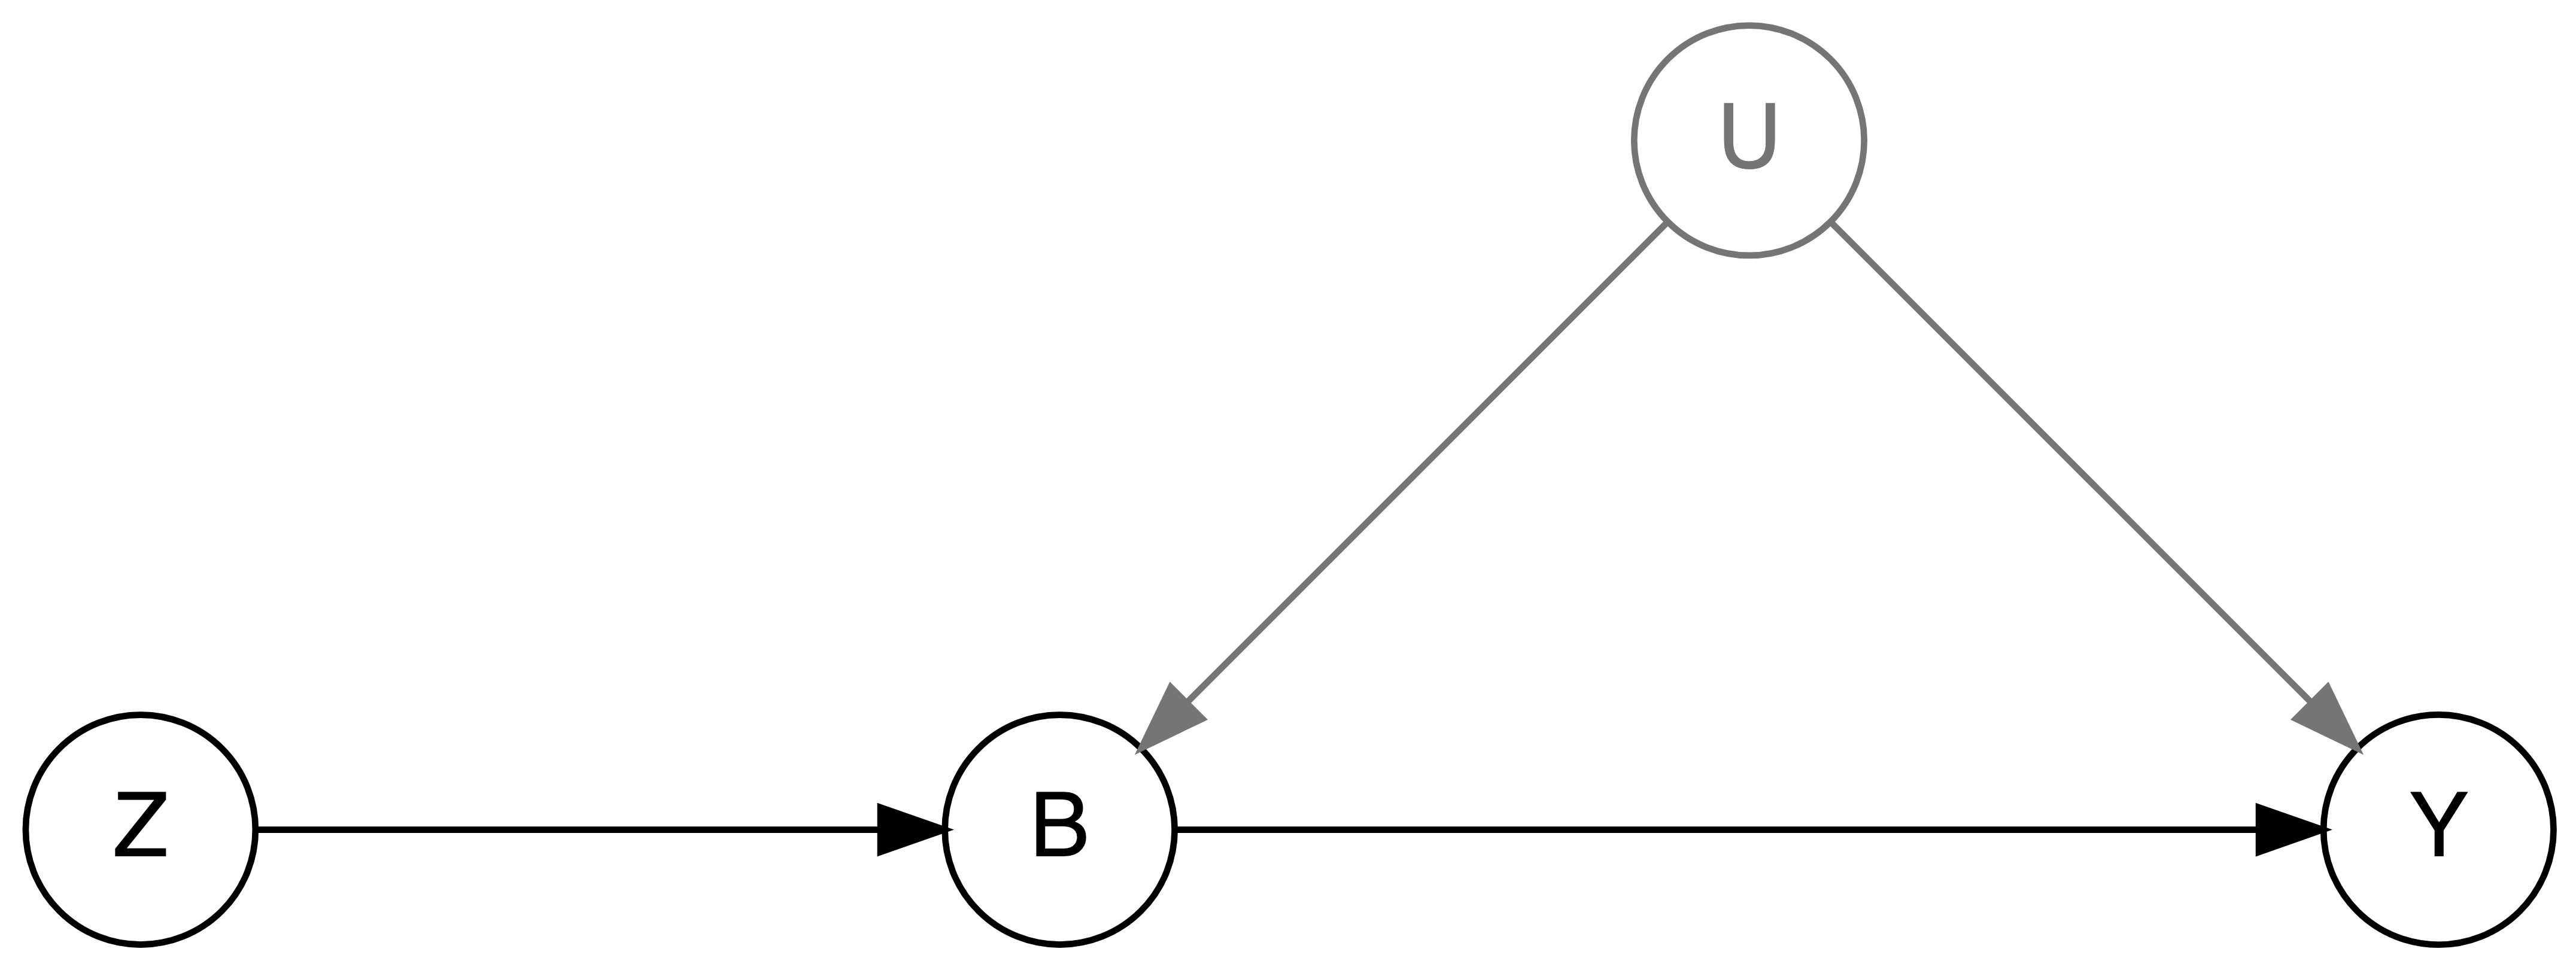
\includegraphics[width=6in,height=4in]{IV_files/figure-latex/dot-figure-1.png}

}

\caption{\label{fig-IVDAG1}IV-Design bei Backdoor durch unb.
Confounder-Variablen}

\end{figure}%

\section{Der einfache lineare
IV-Schätzer}\label{der-einfache-lineare-iv-schuxe4tzer}

Im folgenden nehmen wir an, dass sämtliche Zusammenhänge linear sind.
Zunächst betrachten wir das einfache Regressionsmodell

\begin{align}
  Y_i = \beta_0 + \beta_1 B_i + u_i \ \ , \ \ i=1,\dots,n, \label{eq:simpleiv}
\end{align}

wobei der Fehlerterm \(u_i\) mit dem Regressor \(B_i\) korreliert ist
(d.h. \(B\) ist ein \emph{endogener} Regressor), sodass der KQ-Schätzer
für den kausalen Effekt \(\beta_1\) inkonsistent ist.

Damit \(Z\) ein gültiges Instrument für \(B\) in dem in
Abbildung~\ref{fig-IVDAG1} gezeigten Forschungsdesign ist, müssen die
folgenden Bedingungen erfüllt sein:

Sei \(\text{Cov}(A,B)\) die Kovarianz zwischen den Variablen \(A\) und
\(B\). \(Z\) muss zwei Bedingungen erfüllen, um ein gültiges Instrument
zu sein:

\begin{itemize}
\item
  \textbf{1. Relevanz des Instruments für die endogene Variable}

  \(B\) und \(Z\) \emph{müssen} korreliert sein: \begin{align}
      \text{Cov}(B,Z) \neq 0 \label{eq:ivassum1}
    \end{align}
\item
  \textbf{2. Exogenität des Instruments hinsichtlich der
  Outcome-Variable}

  Das Instrument \(Z\) \emph{darf nicht} mit dem Fehlerterm \(u\) in der
  Modellgleichung \eqref{eq:simpleiv} korreliert sein: \begin{align}
      \text{Cov}(Z,u) = 0 \label{eq:ivassum2}
    \end{align}
\end{itemize}

Unter diesen Annahmen erlaubt das Forschungsdesign die Anwendung des
einfachsten IV-Ansatzes, wobei eine endogene Variable \(B\) durch eine
Instrumentvariable \(Z\) \emph{instrumentiert} wird. Die folgende
Umformung zeigt, warum der kausale Effekt von B auf Y anhand der
(Ko)Variation in diesen Variablen identifiziert werden kann.

\begin{align}
  \textup{Cov}(Z,Y) = &\, \textup{Cov}(Z,\beta_0 + \beta_1 B + u) \tag{Gl. \eqref{eq:simpleiv} einsetzen} \\
  \notag\\
  =&\, \textup{Cov}(Z, \beta_1 B + u) \tag{$\beta_0$ konstant} \\
  \notag\\
  =&\,\, \beta_1\textup{Cov}(Z,B) \tag{IV-Annahme 2} \\
  \notag\\
  \Leftrightarrow \beta_1 =&\, \frac{\textup{Cov}(Z,Y) }{\textup{Cov}(Z,B)} \tag{IV-Annahme 1}
\end{align}

Eine naheliegende Implementierung gemäß dieses Identifikationsprinzips
ist der einfache IV-Schätzer

\begin{align}
  \widehat{\beta}_{\textup{IV}} = \frac{\widehat{\textup{Cov}}(Z,Y) }{\widehat{\textup{Cov}}(Z,B)}, \label{eq:simpleivest}
\end{align}

wobei lediglich die Kovarianzfunktion \(\textup{Cov}(\cdot,\cdot)\)
durch ihr Stichprobenäquivalent \(\widehat{\textup{Cov}}(\cdot,\cdot)\)
ersetzt wird.

\section{2SLS-Verfahren}\label{sls-verfahren}

Der einfache IV-Schätzer \eqref{eq:simpleivest} im Kern ein
Regressionsproblem handelt

\begin{itemize}
\item
  \textbf{1. Stufe: Regression von \(B\) auf \(Z\)}

  Regressiere die endogene Variable \(B\) auf das Instrument \(Z\):
  \begin{align}
      B_i = \alpha_0 + \alpha_1 Z_i + u_i, \quad 1,\dots,n.
    \end{align} Berechne die geschätzten Werte \begin{align}
      \widehat{B}_i = \widehat{\alpha}_0 + \widehat{\alpha}_1 Z_i.
    \end{align}

  Die \(\widehat{B}_i\) aus dieser Regression sind ``bereinigt'': Die
  Variation in den \(\widehat{B}_i\) wird lediglich durch die exogene
  Variation in \(Z\) verursacht.
\item
  \textbf{2. Stufe: Regression von \(Y\) auf \(\widehat{B}\)}

  Regressiere die Beobachtungen der abhängigen Variable \(Y_i\) auf die
  geschätzten Werte \(\widehat{B}_i\) aus der 1. Stufe: \begin{align}
      Y_i = \gamma_0 + \gamma_1 \widehat{B}_i + e_i.
    \end{align} Der geschätzte Koeffizient \(\widehat{\gamma}_1\) aus
  dieser Regression ist der 2SLS-Schätzer von \(\beta_1\)
\end{itemize}

\textbf{Äquivalenz von 2SLS und einfacher IV-Schätzer}

Der KQ-Schätzer von \(\gamma_1\) in der 2. Stufe ist \begin{align}
  \widehat{\gamma}_1 = \frac{\sum (\widehat{B}_i - \overline{\widehat{B}})(Y_i - \bar{Y})}{\sum (\widehat{B}_i - \bar{\widehat{B}})^2}.
\end{align} Da
\(\widehat{B}_i = \widehat{\alpha}_0 + \widehat{\alpha}_1 Z_i\), die
angepassten Werte aus der 1. Stufe, eine lineare Funktion von \(Z_i\)
sind, können wir \(\widehat{\text{Cov}}(\widehat{B}, Y)\) wie folgt
schreiben: \begin{align}
  \widehat{\text{Cov}}(\widehat{B}, Y) = \widehat{\alpha}_1 \widehat{\text{Cov}}(Z, Y)
\end{align} Eine ähnliche Umformung zeigt, dass \begin{align}
  \widehat{\text{Var}}(\widehat{B}) = \widehat{\alpha}_1^2 \widehat{\text{Var}}(Z).
\end{align}

Kombinieren wir diese Ergebnisse, erhalten wir folgende Darstellung für
den KQ-Schätzer von \(\gamma_1\) in der 2. Stufe: \begin{align}
  \widehat{\gamma}_1 = \frac{\widehat{\text{Cov}}(\widehat{B}, Y)}{\widehat{\text{Var}}(\widehat{B})} = \frac{\widehat{\alpha}_1 \widehat{\text{Cov}}(Z, Y)}{\widehat{\alpha}_1^2 \widehat{\text{Var}}(Z)} = \frac{\widehat{\text{Cov}}(Z, Y)}{\widehat{\alpha}_1 \widehat{\text{Var}}(Z)}
\end{align}

Der KQ-Schätzer von \(\widehat{\alpha}_1\) in der 1. Stufe ist definiert
als
\(\widehat{\alpha}_1 = \frac{\widehat{\text{Cov}}(Z, B)}{\widehat{\text{Var}}(Z)}\).
Somit gilt \begin{align}
  \widehat{\gamma}_1 = \frac{\widehat{\text{Cov}}(Z, Y)}{\frac{\widehat{\text{Cov}}(Z, B)}{\widehat{\text{Var}}(Z)} \widehat{\text{Var}}(Z)} = \frac{\widehat{\text{Cov}}(Z, Y)}{\widehat{\text{Cov}}(Z, B)} = \widehat{\beta}_{\textup{IV}}.
\end{align}

In ökonometrischen Softwarepaketen

\begin{center}\rule{0.5\linewidth}{0.5pt}\end{center}

Der im nachfolgenden interaktiven Beispiel betrachtete DGP ist

\begin{align}
  \begin{split}
    X_i =&\, \gamma \cdot Z_i + v_i,\\
    Y_i =&\, \beta_1 \cdot X_i + u_i,
  \end{split}
  \label{eq:OJSIVDGP}
\end{align} wobei \(Z_i \sim N(0, .25^2)\) ist. Die Fehlerterme \(v_i\)
und \(u_i\) sind \(N(0,1)\)-verteilt und folgen einer gemeinsam
Normalverteilung mit Korrelationsparameter \(\rho\), \begin{align}
\begin{pmatrix}
v_i \\ u_i
\end{pmatrix}
\sim N
\bigg[
\begin{pmatrix}
0 \\ 0
\end{pmatrix}
\begin{pmatrix}
1 & \rho \\
\rho & 1
\end{pmatrix}
\bigg].
\end{align}

Wir sind daran interessiert, den Parameter \(\beta_1\) zu schätzen, um
den Effekt von \(X\) auf \(Y\) zu bestimmen, wobei wir \(n=1000\)
Beobachtungen von \((X_i, Y_i, Z_i)\) verwenden.

Beachte, dass \(X_i\) eine Funktion der (exogenen) Variable \(Z_i\) und
des Fehlerterms \(v_i\) ist. Wenn die Fehlerterme \((v_i, u_i)’\) im DGP
\eqref{eq:OJSIVDGP} korreliert sind (\(\rho\neq0\)), dann gibt es eine
Korrelation zwischen \(X_i\) und \(u_i\). Dies impliziert, dass \(X\)
ein endogener Regressor im ``naiven'' Regressionsmodell ist
\begin{align}
Y_i = \beta_0 + \beta_1 X_i + e_i, \quad i = 1,\dots,N,
\end{align} und daher wird der KQ-Schätzer von \(\beta_1\) verzerrt und
inkonsistent sein!

Wenn \(Z\) Erklärungskraft für \(X\) hat, d.h. \(\gamma\neq0\) mit
\(|\gamma|\) nicht zu klein (\(Z\) ist relevant), und \(Z\) nur über
\(X\) auf \(Y\) wirkt (\(Z\) ist exogen in der Gleichung von \(Y_i\)),
dann ist die Instrumentvariablen-Regression eine Möglichkeit,
\(\beta_1\) konsistent zu schätzen.

Zweistufen-Kleinste-Quadrate (2SLS)

\begin{enumerate}
\def\labelenumi{\arabic{enumi}.}
\item
  Erste Stufe: Schätzen Sie das lineare Regressionsmodell

  \begin{align}
   X_i = \alpha_0 + \alpha_1 \cdot Z_i + \epsilon_i
   \end{align} und berechnen Sie die angepassten Werte
  \(\widehat{X}_i\). Dieser Schritt isoliert die exogene Variation in
  \(X_i\), die auf \(Z_i\) zurückzuführen ist.
\item
  Zweite Stufe: Schätzen Sie den Effekt von \(X\) auf \(Y\) unter
  Verwendung von \(\widehat{X}_i\), dem exogenen Teil von \(X_i\) aus
  Schritt 1, mittels der linearen Regression

  \begin{align}
   Y_i = \delta_0 + \delta_1 \cdot \widehat{X}_i  + \varepsilon_i.
   \end{align} Der KQ-Schätzer \(\widehat{\delta}_1\) von \(\delta_1\)
  ist der konsistente 2SLS-Schätzer von \(\beta_1\).
\end{enumerate}

\begin{center}\rule{0.5\linewidth}{0.5pt}\end{center}

\section{Case Study: Ökonomische Schocks und
Bürgerkriege}\label{case-study-uxf6konomische-schocks-und-buxfcrgerkriege}

\texttt{\textasciigrave{}r\ 1+2\textasciigrave{}}

Ein Kernproblem bei der Schätzung der kausalen Beziehung zwischen
wirtschaftlichen Schocks und dem Auftreten von kriegerischen
Auseinandersetzungen ist die Endogenität von Variablen, die
wirtschaftliche Stabilität messen (vgl. Fearon und Laitin 2003).
Beispielsweise kann eine Verschlechterung der wirtschaftlichen
Bedingungen eines Landes die Wahrscheinlichkeit eines Konflikts im
Inland erhöhen. Gleichermaßen beeinflussen kriegerische Handlung im
Inland die wirtschaftliche Situation einer Volkswirtschaft negativ.

\begin{figure}[t]

\centering{

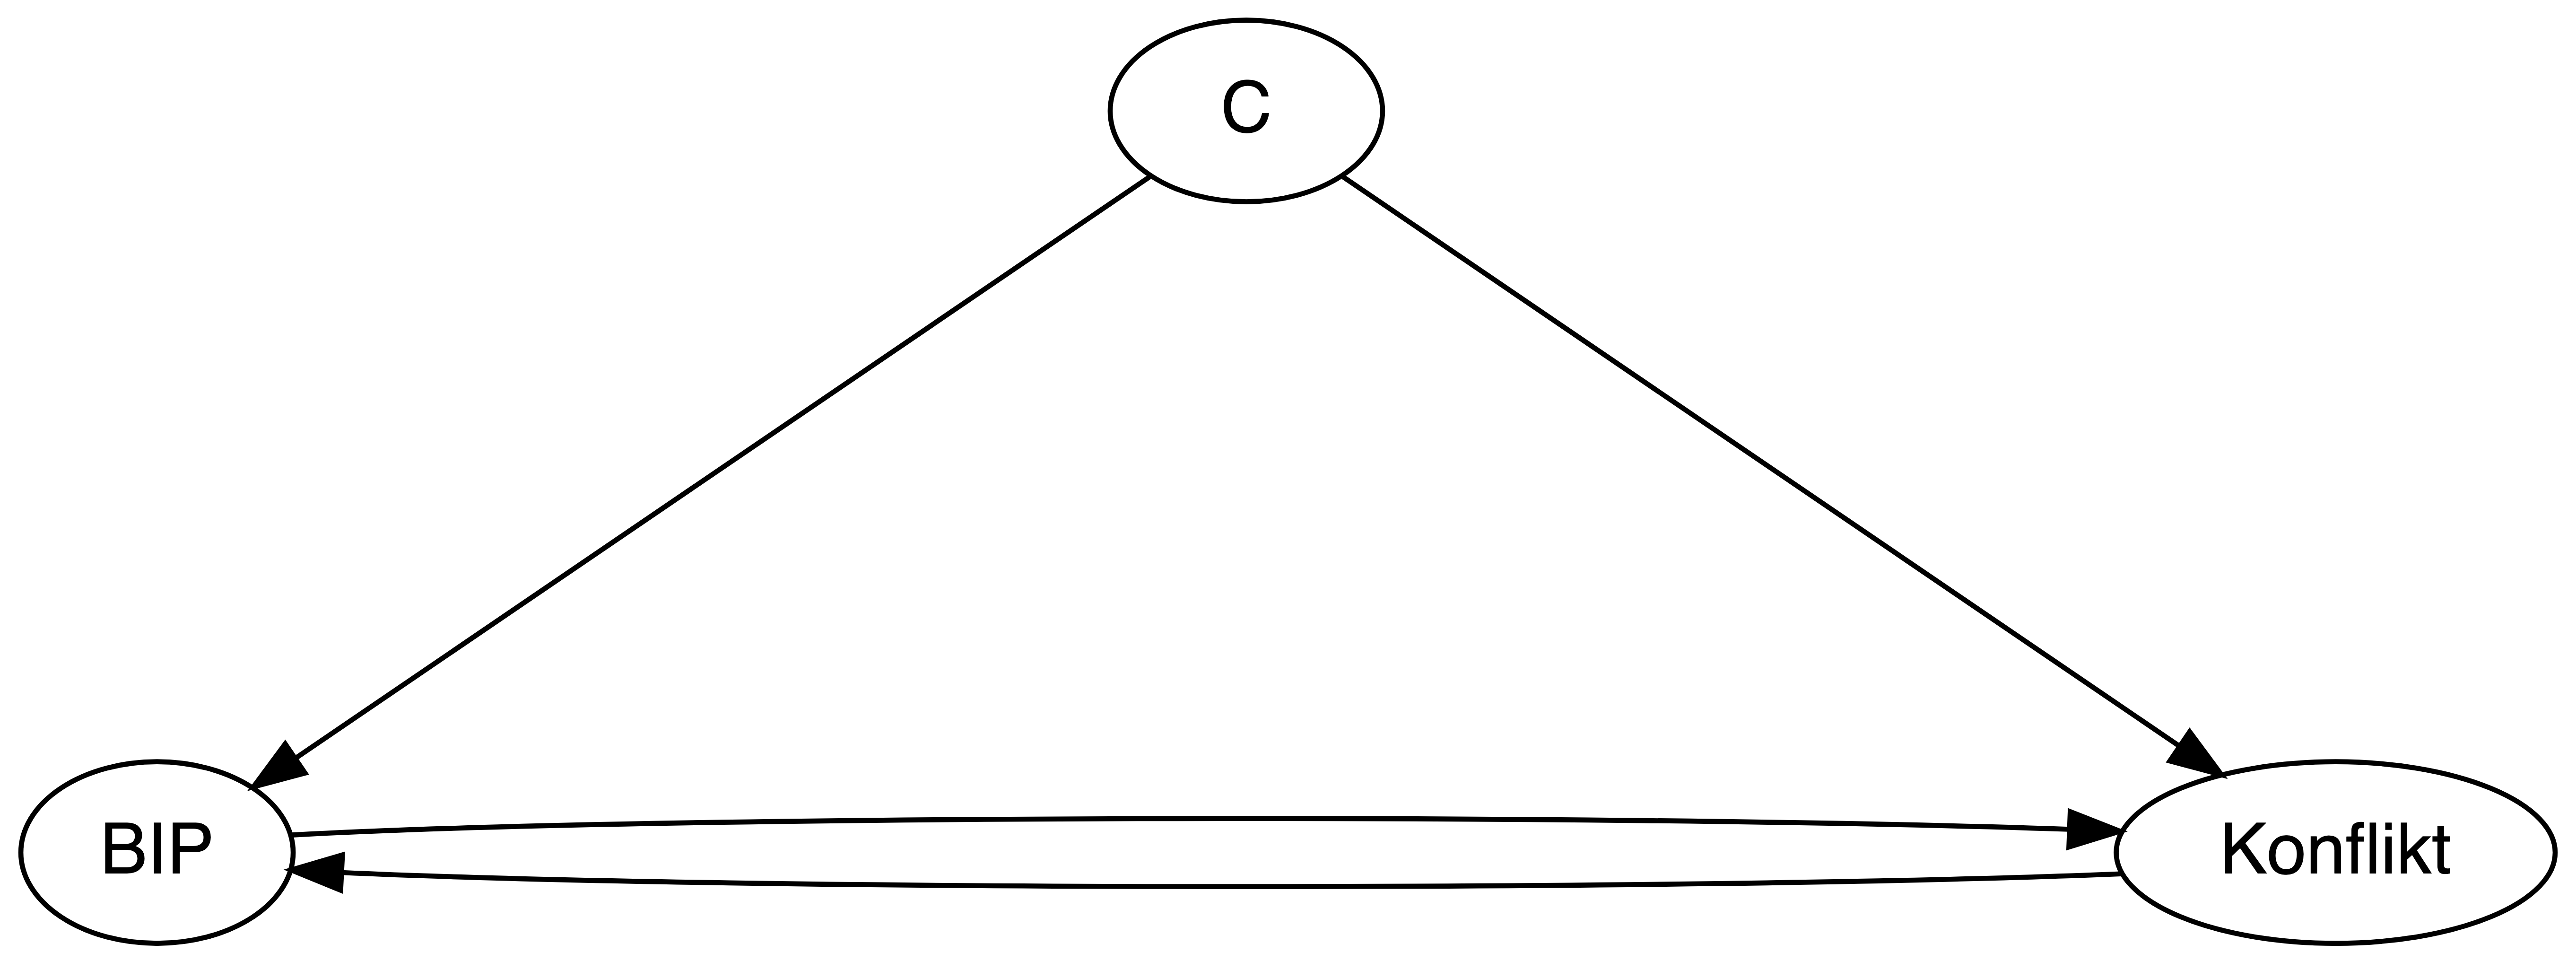
\includegraphics[width=6in,height=4in]{IV_files/figure-latex/dot-figure-3.png}

}

\caption{\label{fig-IVDAGrain1}Simultane Kausalität zw. Kriegsrisiko und
Wirtschaftslage}

\end{figure}%

In der ``Konfliktgleichung''

\begin{align}
  \text{Konflikt-Wsk.} = \beta_0 + \beta_1\, \Delta\text{BIP} + \text{Kontrollv.} + \epsilon\label{eq:rainconf1}
\end{align}

liegt dann Endogenität des Regressors für ``wirtschaftliche
Stabilität'', hier \(\Delta\text{BIP}\), aufgrund von simultanter
Kausalität vor. Die multiple Regression \eqref{eq:rainconf1} liefert
dann eine verzerrte Schätzungen des interessierenden Effekts
\(\beta_1\).

Miguel, Satyanath, und Sergenti (2004) untersuchen die kausale Beziehung
zwischen wirtschaftlichen Schocks und dem Auftreten von Bürgerkriegen in
41 afrikanischen Sub-Sahara-Ländern für den Zeitraum von 1981 bis
1999.\footnote{Siehe
  \texttt{rainconflict\$country\ \%\textgreater{}\%\ unique()}.} Hierbei
adressieren die Autoren das Endogenitätsproblem in einem IV-Ansatz mit
Instrumenten, die mit wirtschaftlichen Schocks korreliert sind, aber
nicht unmittelbar mit der Wahrscheinlichkeit eines Bürgerkriegs
zusammenhängen.

Die Identifikationsstrategie basiert auf metereologischen Faktoren: In
den betrachteten Agrarökonomien sind Schocks in den Niederschlägen
entscheidend für die Entwicklung des Bruttoinlandsprodukts. Ungünstige
Wetterbedingungen, die landwirtschaftliche Erträge negativ beeinflussen,
haben einen direkten (negativen) Effekt auf die wirtschaftliche
Situation. Variation in der Regenmenge ist jedoch keine unmittelbare
Determinante der Konfliktwahrscheinlichkeit und folglich exogen in
Modellgleichung \eqref{eq:rainconf1}. Maße für die Veränderungen in der
Niederschlagsmenge sind somit plausible Instrumente für endogene
Variablen, die Veränderungen im Bruttoinlandsprodukt messen.

\begin{figure}[t]

\centering{

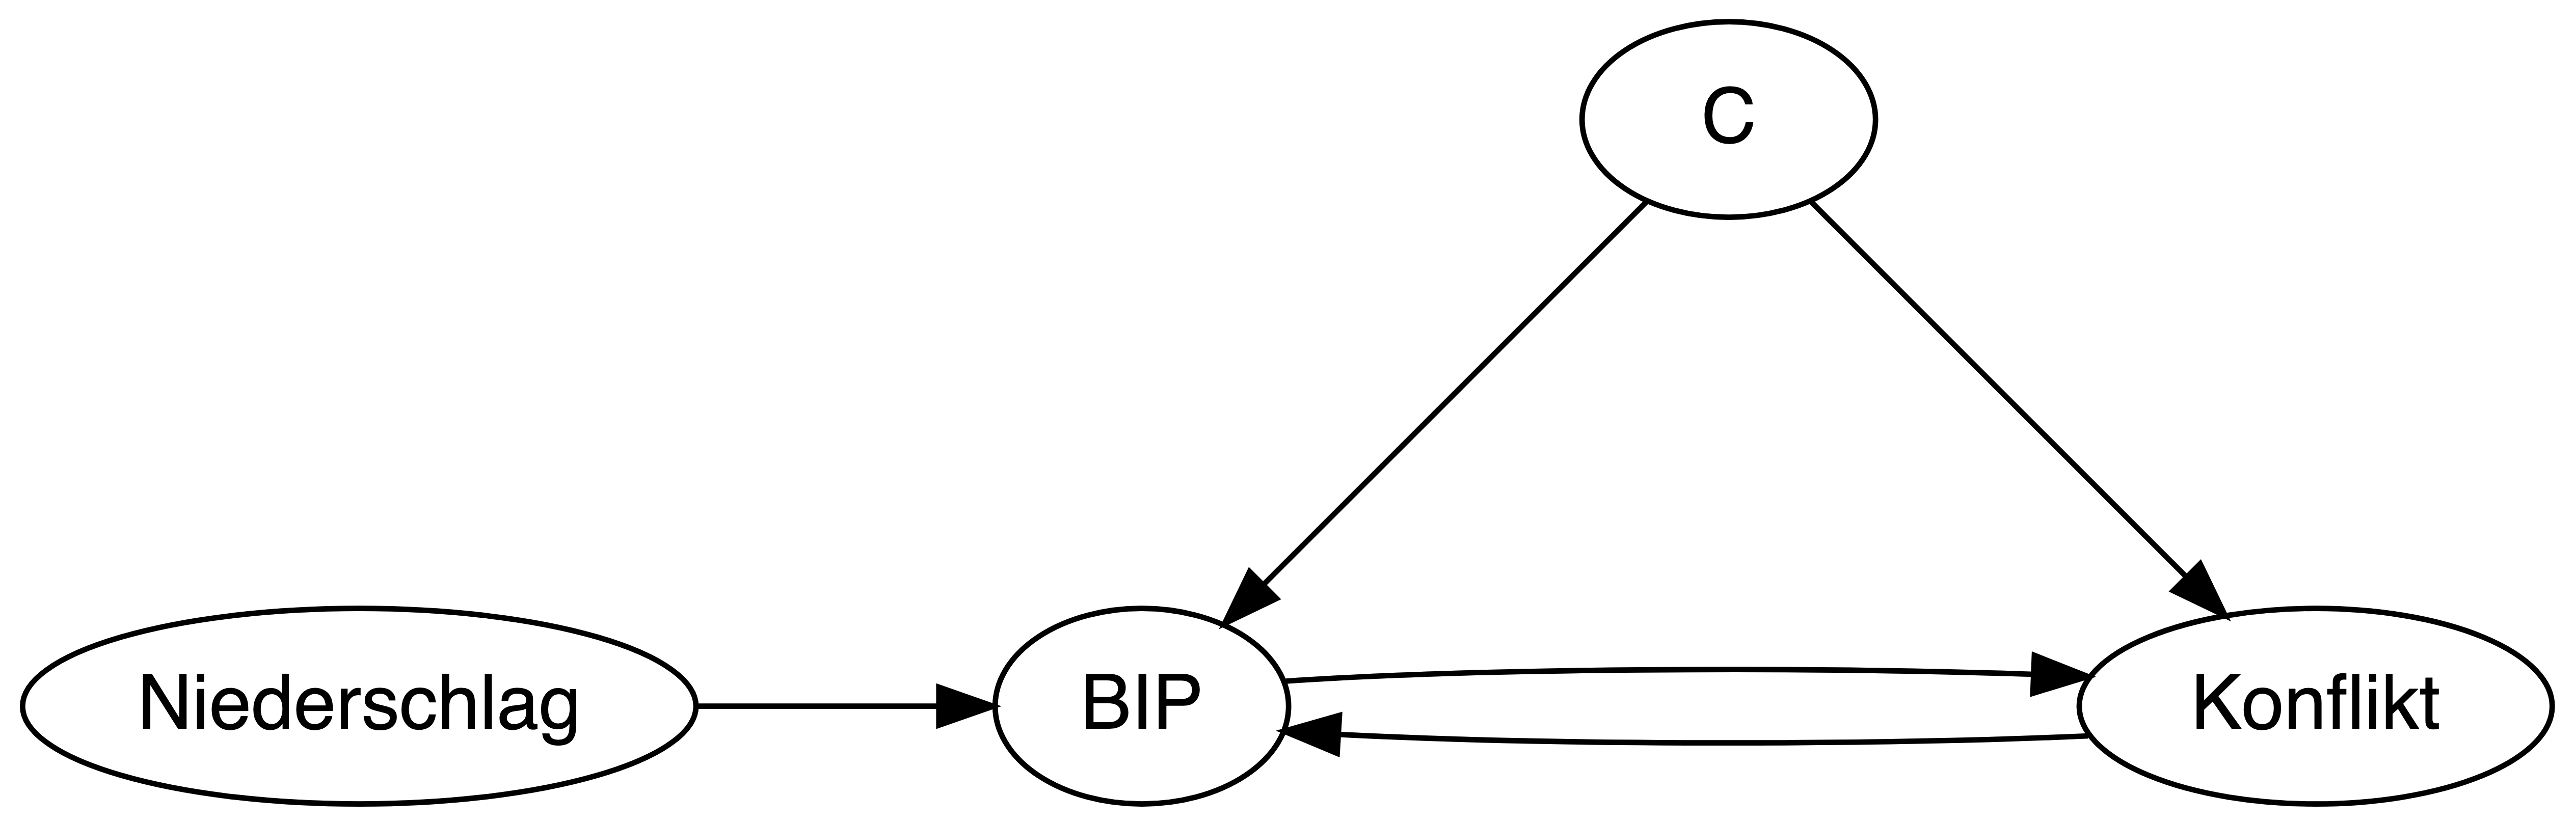
\includegraphics[width=6in,height=4in]{IV_files/figure-latex/dot-figure-2.png}

}

\caption{\label{fig-IVDAGrain2}IV-Design bei simultaner Kausalität zw.
Kriegsrisiko und Wirtschaftslage}

\end{figure}%

Anhand von Länder-Paneldaten mit Informationen über wirtschaftliche
Indikatoren, Konfliktereignisse und Niederschläge, isolieren Miguel,
Satyanath, und Sergenti (2004) in einem IV-Ansatz die exogene Variation
der wirtschaftlichen Entwicklung, d.h. Variation in \(\Delta\text{BIP}\)
die nicht mit dem Fehlerterm in der Konfliktgleichung korreliert ist.
Die Ergebnisse ihrer 2SLS-Schätzungen zeigen, dass negative ökonomische
Schocks die Wahrscheinlichkeit eines Bürgerkriegs signifikant erhöhen.
Miguel, Satyanath, und Sergenti (2004) zeigen weiterhin, dass ihre
Ergebnisse robust gegenüber verschiedenen Modell-Spezifikationen unter
Berücksichtigung diverser Kontrollvariablen sind.

Wir reproduzieren nachfolgend die zentralen Ergebnisse von Miguel,
Satyanath, und Sergenti (2004) anhand eines Auszugs
(\texttt{rainconflict.csv}) aus dem der Studie zugrundeliegenden
Datensatz. Der vollständige Datensatz ist, nach Registrierung,
\href{https://dataverse.harvard.edu/dataset.xhtml?persistentId=doi:10.7910/DVN/27324}{hier}
verfügbar.

\begin{Shaded}
\begin{Highlighting}[]
\FunctionTok{library}\NormalTok{(readr)}

\CommentTok{\# Datensatz \textquotesingle{}rainconflict\textquotesingle{} einlesen}
\NormalTok{rainconflict }\OtherTok{\textless{}{-}} \FunctionTok{read\_csv2}\NormalTok{(}
  \AttributeTok{file =} \StringTok{"datasets/rainconflict.csv"}
\NormalTok{)}
\end{Highlighting}
\end{Shaded}

\begin{Shaded}
\begin{Highlighting}[]
\CommentTok{\# Überblick verschaffen}
\FunctionTok{glimpse}\NormalTok{(rainconflict)}
\end{Highlighting}
\end{Shaded}

\begin{verbatim}
Rows: 743
Columns: 19
$ any_prio   <dbl> 0, 0, 0, 0, 0, 0, 0, 0, 0, 0, 0, 0, 0, 0, 0, 0, 0, 1, 1, 1,~
$ war_prio   <dbl> 0, 0, 0, 0, 0, 0, 0, 0, 0, 0, 0, 0, 0, 0, 0, 0, 0, 1, 0, 0,~
$ ccode      <dbl> 404, 404, 404, 404, 404, 404, 404, 404, 404, 404, 404, 404,~
$ country    <chr> "Guinea-Bissau", "Guinea-Bissau", "Guinea-Bissau", "Guinea-~
$ gdp_g      <dbl> 0.216560572, 0.104712047, -0.042654045, 0.034653414, 0.0366~
$ gdp_g_l    <dbl> -0.152877718, 0.216560572, 0.104712047, -0.042654045, 0.034~
$ GPCP_g     <dbl> 0.170644149, 0.023161817, -0.215036541, 0.098459557, 0.0185~
$ GPCP_g_l   <dbl> -0.048803251, 0.170644149, 0.023161817, -0.215036541, 0.098~
$ GPCP_g_fl  <dbl> 0.023161817, -0.215036541, 0.098459557, 0.018551834, 0.0545~
$ gdp_1979   <dbl> 0.556, 0.556, 0.556, 0.556, 0.556, 0.556, 0.556, 0.556, 0.5~
$ polity2l   <dbl> -7, -7, -7, -7, -8, -8, -8, -8, -8, -8, -6, -6, -6, -6, 5, ~
$ polity2_IV <dbl> -7, -7, -7, -8, -8, -8, -8, -8, -8, -6, -6, -6, -6, 5, 5, 5~
$ ethfrac    <dbl> 0.8037570, 0.8037570, 0.8037570, 0.8037570, 0.8037570, 0.80~
$ relfrac    <dbl> 0.5450, 0.5450, 0.5450, 0.5450, 0.5450, 0.5450, 0.5450, 0.5~
$ oil        <dbl> 0, 0, 0, 0, 0, 0, 0, 0, 0, 0, 0, 0, 0, 0, 0, 0, 0, 0, 0, 0,~
$ lmtnest    <dbl> 0, 0, 0, 0, 0, 0, 0, 0, 0, 0, 0, 0, 0, 0, 0, 0, 0, 0, 0, 0,~
$ lpopl1     <dbl> 6.695799, 6.714170, 6.732211, 6.749931, 6.768493, 6.786717,~
$ tot_100_g  <dbl> 0.3326812088, -0.0604966730, 0.0235692672, 0.6656700373, -0~
$ year       <dbl> 1981, 1982, 1983, 1984, 1985, 1986, 1987, 1988, 1989, 1990,~
\end{verbatim}

\begin{longtable}{ll}

\caption{\label{tbl-rainconfdata}\texttt{rainconflict} --
Polit-ökonomische Charakteristika afrikanischer Länder v. 1981 bis 1999}

\tabularnewline

\toprule
Variable & Beschreibung \\ 
\midrule\addlinespace[2.5pt]
any\_prior & Dummyvariable: Konflikt mit mind. 25 Toten im Jahr t \\ 
war\_prio & Dummyvariable: Konflikt mit mind. 1000 Toten im Jahr t \\ 
ccode & Länderkennung (numerisch) \\ 
country & Name des Landes \\ 
gdp\_g & (BIP\_t - BIP\_t-1) / BIP\_t-1 \\ 
gdp\_g\_l & (BIP\_t-1 - BIP\_t-2) / BIP\_t-2 \\ 
GPCP\_g & (Niederschlag\_t - Niederschlag\_t-1) / Niederschlag\_t-1 \\ 
GPCP\_g\_l & GPCP\_g in t-1 \\ 
GPCP\_g\_fl & GPCP\_g in t+1 \\ 
gdp\_1979 & Log Pro-Kopf-BIP in 1979 \\ 
polity2\_IV & Diff. zw. Demokratie- und Autokrarie-Score im Jahr t (Skala v. -10 bis 10) \\ 
polity2l & polity2\_IV im Jahr t-1 (Skala v. -10 bis 10) \\ 
ethfrac & Ethno-linguistische Fragmentierung (Anteil) \\ 
relfrac & Religiöse Fragmentierung (Anteil) \\ 
oil & Dummy für Öl-exportierendes Land \\ 
lmtnest & Log Anteil Gebirgsregionen an Landesfläche \\ 
lpopl1 & Log Bevölkerung im Jahr t-1 \\ 
tot\_100\_g & Handelsbedingungen (Index, 1995 = 100) \\ 
year & Jahr der Beobachtung \\ 
\bottomrule

\end{longtable}

\begin{Shaded}
\begin{Highlighting}[]
\CommentTok{\# ccode zu Typ \textquotesingle{}factor\textquotesingle{} transformieren}
\NormalTok{rainconflict }\OtherTok{\textless{}{-}}\NormalTok{ rainconflict }\SpecialCharTok{\%\textgreater{}\%} 
  \FunctionTok{mutate}\NormalTok{(}
    \AttributeTok{ccode =} \FunctionTok{as.factor}\NormalTok{(ccode)}
\NormalTok{  )}
\end{Highlighting}
\end{Shaded}

\begin{Shaded}
\begin{Highlighting}[]
\FunctionTok{library}\NormalTok{(modelsummary)}

\CommentTok{\# Statistische Zusammenfassung}
\FunctionTok{datasummary}\NormalTok{(}
  \AttributeTok{formula =} \FunctionTok{All}\NormalTok{( rainconflict }\SpecialCharTok{\%\textgreater{}\%} \FunctionTok{select}\NormalTok{(}\SpecialCharTok{{-}}\NormalTok{ccode, }\SpecialCharTok{{-}}\NormalTok{year) )   }
    \SpecialCharTok{\textasciitilde{}}\NormalTok{ (mean }\SpecialCharTok{+}\NormalTok{ sd) }\SpecialCharTok{*} \FunctionTok{Arguments}\NormalTok{(}\AttributeTok{na.rm =} \ConstantTok{TRUE}\NormalTok{) }
    \SpecialCharTok{+}\NormalTok{ N, }
  \AttributeTok{fmt =} \DecValTok{4}\NormalTok{,}
  \AttributeTok{data =}\NormalTok{ rainconflict }
\NormalTok{) }
\end{Highlighting}
\end{Shaded}

\begin{table}

\caption{\label{tbl-rainconfdatasum}\texttt{rainconflict} --
Statistische Zusammenfassung}

\centering{

\centering
\begin{tblr}[         %% tabularray outer open
]                     %% tabularray outer close
{                     %% tabularray inner open
colspec={Q[]Q[]Q[]Q[]},
column{1}={halign=l,},
column{2}={halign=r,},
column{3}={halign=r,},
column{4}={halign=r,},
}                     %% tabularray inner close
\toprule
& mean & sd & N \\ \midrule %% TinyTableHeader
any\_prio    & \num{0.2678}  & \num{0.4431} & 743 \\
war\_prio    & \num{0.1669}  & \num{0.3731} & 743 \\
gdp\_g       & \num{-0.0048} & \num{0.0707} & 743 \\
gdp\_g\_l   & \num{-0.0056} & \num{0.0724} & 743 \\
GPCP\_g      & \num{0.0182}  & \num{0.2094} & 743 \\
GPCP\_g\_l  & \num{0.0113}  & \num{0.2067} & 743 \\
GPCP\_g\_fl & \num{0.0150}  & \num{0.2107} & 743 \\
gdp\_1979    & \num{1.1639}  & \num{0.9009} & 743 \\
polity2l      & \num{-3.6083} & \num{5.5543} & 743 \\
polity2\_IV  & \num{-3.4035} & \num{5.5766} & 736 \\
ethfrac       & \num{0.6546}  & \num{0.2374} & 743 \\
relfrac       & \num{0.4868}  & \num{0.1857} & 743 \\
oil           & \num{0.1184}  & \num{0.3233} & 743 \\
lmtnest       & \num{1.5783}  & \num{1.4334} & 743 \\
lpopl1        & \num{8.7497}  & \num{1.2068} & 743 \\
tot\_100\_g & \num{-0.0068} & \num{0.1552} & 661 \\
\bottomrule
\end{tblr}

}

\end{table}%

\begin{Shaded}
\begin{Highlighting}[]
\FunctionTok{library}\NormalTok{(fixest)}

\CommentTok{\# (1)}
\NormalTok{(}
\NormalTok{  rncnf\_mod1 }\OtherTok{\textless{}{-}} \FunctionTok{feols}\NormalTok{(}
    \AttributeTok{fml =}\NormalTok{ gdp\_g }\SpecialCharTok{\textasciitilde{}}\NormalTok{ GPCP\_g }\SpecialCharTok{+}\NormalTok{ GPCP\_g\_l,}
    \AttributeTok{data =}\NormalTok{ rainconflict,}
    \AttributeTok{vcov =} \SpecialCharTok{\textasciitilde{}}\NormalTok{ ccode}
\NormalTok{  )}
\NormalTok{)}
\end{Highlighting}
\end{Shaded}

\begin{verbatim}
OLS estimation, Dep. Var.: gdp_g
Observations: 743
Standard-errors: Clustered (ccode) 
             Estimate Std. Error  t value  Pr(>|t|)    
(Intercept) -0.006147   0.002460 -2.49856 0.0166787 *  
GPCP_g       0.055430   0.016301  3.40029 0.0015378 ** 
GPCP_g_l     0.034058   0.013213  2.57761 0.0137398 *  
---
Signif. codes:  0 '***' 0.001 '**' 0.01 '*' 0.05 '.' 0.1 ' ' 1
RMSE: 0.069815   Adj. R2: 0.02088
\end{verbatim}

\begin{Shaded}
\begin{Highlighting}[]
\CommentTok{\# (2)}
\NormalTok{rncnf\_mod2 }\OtherTok{\textless{}{-}} \FunctionTok{feols}\NormalTok{(}
  \AttributeTok{fml =}\NormalTok{ gdp\_g }\SpecialCharTok{\textasciitilde{}}\NormalTok{ GPCP\_g }\SpecialCharTok{+}\NormalTok{ GPCP\_g\_l}
  \SpecialCharTok{+}\NormalTok{ gdp\_1979}
  \SpecialCharTok{+}\NormalTok{ polity2l }
  \SpecialCharTok{+}\NormalTok{ ethfrac }
  \SpecialCharTok{+}\NormalTok{ relfrac }
  \SpecialCharTok{+}\NormalTok{ oil }
  \SpecialCharTok{+}\NormalTok{ lmtnest }
  \SpecialCharTok{+}\NormalTok{ lpopl1}
  \SpecialCharTok{+}\NormalTok{ year}\SpecialCharTok{:}\NormalTok{ccode,}
  \AttributeTok{data =}\NormalTok{ rainconflict,}
  \AttributeTok{vcov =} \SpecialCharTok{\textasciitilde{}}\NormalTok{ ccode}
\NormalTok{) }

\NormalTok{rncnf\_mod2 }\SpecialCharTok{\%\textgreater{}\%} 
  \FunctionTok{print}\NormalTok{(}\AttributeTok{n =} \DecValTok{10}\NormalTok{)}
\end{Highlighting}
\end{Shaded}

\begin{verbatim}
OLS estimation, Dep. Var.: gdp_g
Observations: 743
Standard-errors: Clustered (ccode) 
             Estimate Std. Error   t value  Pr(>|t|)    
(Intercept) -8.380394   7.836789 -1.069366 0.2913157    
GPCP_g       0.053402   0.016788  3.180892 0.0028359 ** 
GPCP_g_l     0.031518   0.013739  2.294105 0.0271135 *  
gdp_1979    -0.568562   0.933728 -0.608916 0.5460230    
polity2l    -0.000462   0.000697 -0.661827 0.5118772    
ethfrac     -0.290995   5.315419 -0.054745 0.9566138    
relfrac      6.344474   6.277193  1.010718 0.3182264    
oil         -0.022946   0.011735 -1.955363 0.0575517 .  
lmtnest     -0.154883   0.950072 -0.163022 0.8713219    
lpopl1      -0.103898   0.140671 -0.738588 0.4644693    
... 41 coefficients remaining
---
Signif. codes:  0 '***' 0.001 '**' 0.01 '*' 0.05 '.' 0.1 ' ' 1
RMSE: 0.067787   Adj. R2: 0.012893
\end{verbatim}

\begin{Shaded}
\begin{Highlighting}[]
\CommentTok{\# (3)}
\NormalTok{rncnf\_mod3 }\OtherTok{\textless{}{-}} \FunctionTok{feols}\NormalTok{(}
  \AttributeTok{fml =}\NormalTok{ gdp\_g }\SpecialCharTok{\textasciitilde{}}\NormalTok{ GPCP\_g }\SpecialCharTok{+}\NormalTok{ GPCP\_g\_l }
  \SpecialCharTok{+}\NormalTok{ year}\SpecialCharTok{:}\NormalTok{ccode}
  \SpecialCharTok{|}\NormalTok{ ccode,}
  \AttributeTok{data =}\NormalTok{ rainconflict,}
  \AttributeTok{vcov =} \SpecialCharTok{\textasciitilde{}}\NormalTok{ ccode}
\NormalTok{) }

\NormalTok{rncnf\_mod3 }\SpecialCharTok{\%\textgreater{}\%} 
  \FunctionTok{print}\NormalTok{(}\AttributeTok{n =} \DecValTok{2}\NormalTok{)}
\end{Highlighting}
\end{Shaded}

\begin{verbatim}
OLS estimation, Dep. Var.: gdp_g
Observations: 743
Fixed-effects: ccode: 41
Standard-errors: Clustered (ccode) 
         Estimate Std. Error t value  Pr(>|t|)    
GPCP_g   0.048582   0.016523 2.94024 0.0054275 ** 
GPCP_g_l 0.028004   0.013779 2.03236 0.0487938 *  
... 41 coefficients remaining
---
Signif. codes:  0 '***' 0.001 '**' 0.01 '*' 0.05 '.' 0.1 ' ' 1
RMSE: 0.065802     Adj. R2: 0.023299
                 Within R2: 0.086915
\end{verbatim}

\begin{Shaded}
\begin{Highlighting}[]
\CommentTok{\# (4)}
\NormalTok{rncnf\_mod4 }\OtherTok{\textless{}{-}} \FunctionTok{feols}\NormalTok{(}
  \AttributeTok{fml =}\NormalTok{ gdp\_g }\SpecialCharTok{\textasciitilde{}}\NormalTok{ GPCP\_g }\SpecialCharTok{+}\NormalTok{ GPCP\_g\_l }\SpecialCharTok{+}\NormalTok{ GPCP\_g\_fl}
  \SpecialCharTok{+}\NormalTok{ year}\SpecialCharTok{:}\NormalTok{ccode }
  \SpecialCharTok{|}\NormalTok{ ccode,}
  \AttributeTok{data =}\NormalTok{ rainconflict,}
  \AttributeTok{vcov =} \SpecialCharTok{\textasciitilde{}}\NormalTok{ ccode}
\NormalTok{) }

\NormalTok{rncnf\_mod4 }\SpecialCharTok{\%\textgreater{}\%} 
  \FunctionTok{print}\NormalTok{(}\AttributeTok{n =} \DecValTok{3}\NormalTok{)}
\end{Highlighting}
\end{Shaded}

\begin{verbatim}
OLS estimation, Dep. Var.: gdp_g
Observations: 743
Fixed-effects: ccode: 41
Standard-errors: Clustered (ccode) 
          Estimate Std. Error  t value  Pr(>|t|)    
GPCP_g    0.048944   0.017837 2.743919 0.0090443 ** 
GPCP_g_l  0.028235   0.013783 2.048544 0.0471081 *  
GPCP_g_fl 0.000617   0.018501 0.033337 0.9735719    
... 41 coefficients remaining
---
Signif. codes:  0 '***' 0.001 '**' 0.01 '*' 0.05 '.' 0.1 ' ' 1
RMSE: 0.065801     Adj. R2: 0.021818
                 Within R2: 0.086917
\end{verbatim}

\begin{Shaded}
\begin{Highlighting}[]
\CommentTok{\# (5)}
\NormalTok{rncnf\_mod5 }\OtherTok{\textless{}{-}} \FunctionTok{feols}\NormalTok{(}
  \AttributeTok{fml =}\NormalTok{ gdp\_g }\SpecialCharTok{\textasciitilde{}}\NormalTok{ GPCP\_g }\SpecialCharTok{+}\NormalTok{ GPCP\_g\_l }
  \SpecialCharTok{+}\NormalTok{ tot\_100\_g }
  \SpecialCharTok{+}\NormalTok{ year}\SpecialCharTok{:}\NormalTok{ccode }
  \SpecialCharTok{|}\NormalTok{ ccode,}
  \AttributeTok{data =}\NormalTok{ rainconflict,}
  \AttributeTok{vcov =} \SpecialCharTok{\textasciitilde{}}\NormalTok{ ccode}
\NormalTok{) }

\NormalTok{rncnf\_mod5 }\SpecialCharTok{\%\textgreater{}\%}
  \FunctionTok{print}\NormalTok{(}\AttributeTok{n =} \DecValTok{3}\NormalTok{)}
\end{Highlighting}
\end{Shaded}

\begin{verbatim}
OLS estimation, Dep. Var.: gdp_g
Observations: 661
Fixed-effects: ccode: 37
Standard-errors: Clustered (ccode) 
           Estimate Std. Error   t value  Pr(>|t|)    
GPCP_g     0.053124   0.017432  3.047509 0.0043049 ** 
GPCP_g_l   0.036616   0.014705  2.490060 0.0175258 *  
tot_100_g -0.002280   0.022286 -0.102318 0.9190722    
... 37 coefficients remaining
---
Signif. codes:  0 '***' 0.001 '**' 0.01 '*' 0.05 '.' 0.1 ' ' 1
RMSE: 0.059582     Adj. R2: 0.052542
                 Within R2: 0.114693
\end{verbatim}

\begin{Shaded}
\begin{Highlighting}[]
\CommentTok{\# Tabellarischer Vergleich mit modelsummary()}
\CommentTok{\# (Tabelle 3 in Ditella und Schargrodsky, 2004)}
\FunctionTok{modelsummary}\NormalTok{(}
  \AttributeTok{models =} \FunctionTok{list}\NormalTok{(}
    \StringTok{"(1)"} \OtherTok{=}\NormalTok{ rncnf\_mod1, }
    \StringTok{"(2)"} \OtherTok{=}\NormalTok{ rncnf\_mod2, }
    \StringTok{"(3)"} \OtherTok{=}\NormalTok{ rncnf\_mod3, }
    \StringTok{"(4)"} \OtherTok{=}\NormalTok{ rncnf\_mod4, }
    \StringTok{"(5)"} \OtherTok{=}\NormalTok{ rncnf\_mod5}
\NormalTok{  ),}
  \AttributeTok{stars =}\NormalTok{ T, }
  \AttributeTok{coef\_omit =} \StringTok{"\^{}year.*$"}\NormalTok{,}
  \AttributeTok{gof\_omit =} \StringTok{"\^{}(?!(R2|Num.Obs.|FE.*)$).*"}\NormalTok{, }
  \AttributeTok{output =} \StringTok{"gt"}
\NormalTok{)}
\end{Highlighting}
\end{Shaded}

\setlength{\LTpost}{0mm}

\begin{longtable}{lccccc}

\caption{\label{tbl-blablabla}First-Stage-Regressionen für
\texttt{gdp\_g}}

\tabularnewline

\toprule
  & (1) & (2) & (3) & (4) & (5) \\ 
\midrule\addlinespace[2.5pt]
(Intercept) & -0.006* & -8.380 &  &  &  \\ 
 & (0.002) & (7.837) &  &  &  \\ 
GPCP\_g & 0.055** & 0.053** & 0.049** & 0.049** & 0.053** \\ 
 & (0.016) & (0.017) & (0.017) & (0.018) & (0.017) \\ 
GPCP\_g\_l & 0.034* & 0.032* & 0.028* & 0.028* & 0.037* \\ 
 & (0.013) & (0.014) & (0.014) & (0.014) & (0.015) \\ 
gdp\_1979 &  & -0.569 &  &  &  \\ 
 &  & (0.934) &  &  &  \\ 
polity2l &  & 0.000 &  &  &  \\ 
 &  & (0.001) &  &  &  \\ 
ethfrac &  & -0.291 &  &  &  \\ 
 &  & (5.315) &  &  &  \\ 
relfrac &  & 6.344 &  &  &  \\ 
 &  & (6.277) &  &  &  \\ 
oil &  & -0.023+ &  &  &  \\ 
 &  & (0.012) &  &  &  \\ 
lmtnest &  & -0.155 &  &  &  \\ 
 &  & (0.950) &  &  &  \\ 
lpopl1 &  & -0.104 &  &  &  \\ 
 &  & (0.141) &  &  &  \\ 
GPCP\_g\_fl &  &  &  & 0.001 &  \\ 
 &  &  &  & (0.019) &  \\ 
tot\_100\_g &  &  &  &  & -0.002 \\ 
 &  &  &  &  & (0.022) \\ 
Num.Obs. & 743 & 743 & 743 & 743 & 661 \\ 
R2 & 0.024 & 0.079 & 0.133 & 0.133 & 0.162 \\ 
FE: ccode &  &  & X & X & X \\ 
\bottomrule

\end{longtable}

\begin{minipage}{\linewidth}
+ p < 0.1, * p < 0.05, ** p < 0.01, *** p < 0.001\\
\end{minipage}

\begin{Shaded}
\begin{Highlighting}[]
\NormalTok{S1\_res }\OtherTok{\textless{}{-}} \FunctionTok{tibble}\NormalTok{(}

  \AttributeTok{x =} \FunctionTok{residuals}\NormalTok{(}
    \FunctionTok{feols}\NormalTok{(}
      \AttributeTok{fml =}\NormalTok{ GPCP\_g }\SpecialCharTok{\textasciitilde{}}\NormalTok{ GPCP\_g\_l}
      \SpecialCharTok{+}\NormalTok{ year}\SpecialCharTok{:}\NormalTok{ccode}
      \SpecialCharTok{|}\NormalTok{ ccode,}
      \AttributeTok{data =}\NormalTok{ rainconflict}
\NormalTok{    )}
\NormalTok{  ),}
  
  \AttributeTok{y =} \FunctionTok{residuals}\NormalTok{(}
    \FunctionTok{feols}\NormalTok{(}
      \AttributeTok{fml =}\NormalTok{ gdp\_g }\SpecialCharTok{\textasciitilde{}}\NormalTok{ GPCP\_g\_l}
      \SpecialCharTok{+}\NormalTok{ year}\SpecialCharTok{:}\NormalTok{ccode}
      \SpecialCharTok{|}\NormalTok{ ccode,}
      \AttributeTok{data =}\NormalTok{ rainconflict}
\NormalTok{    )}
\NormalTok{  )}
  
\NormalTok{)}
\end{Highlighting}
\end{Shaded}

\begin{Shaded}
\begin{Highlighting}[]
\FunctionTok{library}\NormalTok{(ggplot2)}
\FunctionTok{library}\NormalTok{(cowplot)}

\FunctionTok{ggplot}\NormalTok{(}
  \AttributeTok{data =}\NormalTok{ S1\_res,}
  \AttributeTok{mapping =} \FunctionTok{aes}\NormalTok{(}\AttributeTok{x =}\NormalTok{ x, }\AttributeTok{y =}\NormalTok{ y)) }\SpecialCharTok{+}
  \FunctionTok{geom\_point}\NormalTok{(}
    \AttributeTok{size =}\NormalTok{ .}\DecValTok{75}\NormalTok{, }
    \AttributeTok{alpha =}\NormalTok{ .}\DecValTok{5}
\NormalTok{  ) }\SpecialCharTok{+}
  \FunctionTok{geom\_smooth}\NormalTok{(}\AttributeTok{method =} \StringTok{"loess"}\NormalTok{, }\AttributeTok{span =}\NormalTok{ .}\DecValTok{5}\NormalTok{) }\SpecialCharTok{+}
  \FunctionTok{coord\_cartesian}\NormalTok{(}
    \AttributeTok{xlim =} \FunctionTok{c}\NormalTok{(}\SpecialCharTok{{-}}\NormalTok{.}\DecValTok{4}\NormalTok{, .}\DecValTok{4}\NormalTok{), }
    \AttributeTok{ylim =} \FunctionTok{c}\NormalTok{(}\SpecialCharTok{{-}}\NormalTok{.}\DecValTok{1}\NormalTok{, .}\DecValTok{1}\NormalTok{)}
\NormalTok{  ) }\SpecialCharTok{+}
  \FunctionTok{theme\_cowplot}\NormalTok{()}
\end{Highlighting}
\end{Shaded}

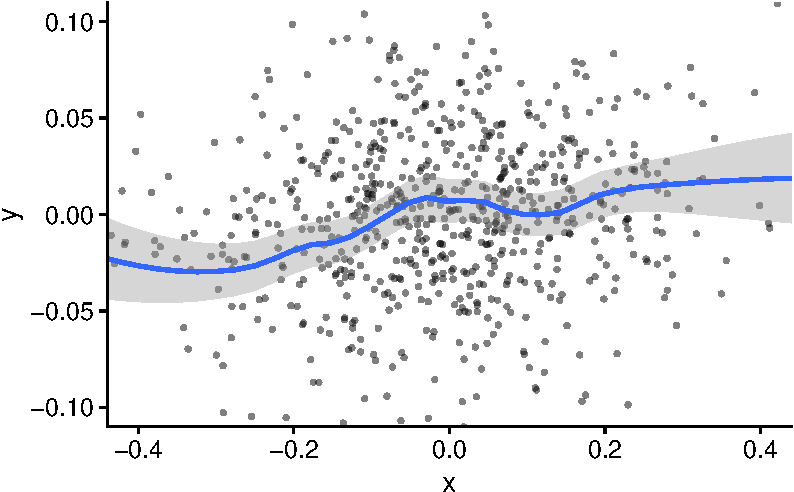
\includegraphics{IV_files/figure-pdf/unnamed-chunk-17-1.pdf}

\begin{Shaded}
\begin{Highlighting}[]
\FunctionTok{feols}\NormalTok{(}
  \AttributeTok{fml =}\NormalTok{ any\_prio }\SpecialCharTok{\textasciitilde{}}\NormalTok{ GPCP\_g }\SpecialCharTok{+}\NormalTok{ GPCP\_g\_l }
  \SpecialCharTok{+}\NormalTok{ year}\SpecialCharTok{:}\NormalTok{ccode}
  \SpecialCharTok{|}\NormalTok{ ccode,}
  \AttributeTok{data =}\NormalTok{ rainconflict,}
  \AttributeTok{vcov =} \SpecialCharTok{\textasciitilde{}}\NormalTok{ ccode}
\NormalTok{) }\SpecialCharTok{\%\textgreater{}\%} 
  \FunctionTok{print}\NormalTok{(}\AttributeTok{n =} \DecValTok{2}\NormalTok{)}
\end{Highlighting}
\end{Shaded}

\begin{verbatim}
OLS estimation, Dep. Var.: any_prio
Observations: 743
Fixed-effects: ccode: 41
Standard-errors: Clustered (ccode) 
          Estimate Std. Error   t value Pr(>|t|)    
GPCP_g   -0.023770   0.041969 -0.566373  0.57430    
GPCP_g_l -0.121936   0.050328 -2.422836  0.02002 *  
... 41 coefficients remaining
---
Signif. codes:  0 '***' 0.001 '**' 0.01 '*' 0.05 '.' 0.1 ' ' 1
RMSE: 0.239168     Adj. R2: 0.671564
                 Within R2: 0.374052
\end{verbatim}

\begin{Shaded}
\begin{Highlighting}[]
\FunctionTok{feols}\NormalTok{(}
  \AttributeTok{fml =}\NormalTok{ war\_prio }\SpecialCharTok{\textasciitilde{}}\NormalTok{ GPCP\_g }\SpecialCharTok{+}\NormalTok{ GPCP\_g\_l }
  \SpecialCharTok{+}\NormalTok{ year}\SpecialCharTok{:}\NormalTok{ccode}
  \SpecialCharTok{|}\NormalTok{ ccode,}
  \AttributeTok{data =}\NormalTok{ rainconflict,}
  \AttributeTok{vcov =} \SpecialCharTok{\textasciitilde{}}\NormalTok{ ccode}
\NormalTok{) }\SpecialCharTok{\%\textgreater{}\%} 
  \FunctionTok{print}\NormalTok{(}\AttributeTok{n =} \DecValTok{2}\NormalTok{)}
\end{Highlighting}
\end{Shaded}

\begin{verbatim}
OLS estimation, Dep. Var.: war_prio
Observations: 743
Fixed-effects: ccode: 41
Standard-errors: Clustered (ccode) 
          Estimate Std. Error  t value Pr(>|t|)    
GPCP_g   -0.062476   0.029051 -2.15060 0.037605 *  
GPCP_g_l -0.068689   0.030678 -2.23904 0.030783 *  
... 41 coefficients remaining
---
Signif. codes:  0 '***' 0.001 '**' 0.01 '*' 0.05 '.' 0.1 ' ' 1
RMSE: 0.204541     Adj. R2: 0.661198
                 Within R2: 0.385205
\end{verbatim}

\begin{Shaded}
\begin{Highlighting}[]
\NormalTok{rf\_res }\OtherTok{\textless{}{-}} \FunctionTok{tibble}\NormalTok{(}
  
  \AttributeTok{x =} \FunctionTok{residuals}\NormalTok{(}
    \FunctionTok{feols}\NormalTok{(}
      \AttributeTok{fml =}\NormalTok{ GPCP\_g\_l }\SpecialCharTok{\textasciitilde{}}\NormalTok{ GPCP\_g}
      \SpecialCharTok{+}\NormalTok{ year}\SpecialCharTok{:}\NormalTok{ccode}
      \SpecialCharTok{|}\NormalTok{ ccode,}
      \AttributeTok{data =}\NormalTok{ rainconflict}
\NormalTok{    )}
\NormalTok{  ),}
  
  \AttributeTok{y =} \FunctionTok{residuals}\NormalTok{(}
    \FunctionTok{feols}\NormalTok{(}
      \AttributeTok{fml =}\NormalTok{ any\_prio }\SpecialCharTok{\textasciitilde{}}\NormalTok{ GPCP\_g}
      \SpecialCharTok{+}\NormalTok{ year}\SpecialCharTok{:}\NormalTok{ccode}
      \SpecialCharTok{|}\NormalTok{ ccode,}
      \AttributeTok{data =}\NormalTok{ rainconflict}
\NormalTok{    )}
\NormalTok{  )}
  
\NormalTok{)}
\end{Highlighting}
\end{Shaded}

\begin{Shaded}
\begin{Highlighting}[]
\FunctionTok{ggplot}\NormalTok{(}
  \AttributeTok{data =}\NormalTok{ rf\_res , }
  \AttributeTok{mapping =} \FunctionTok{aes}\NormalTok{(}\AttributeTok{x =}\NormalTok{ x, }\AttributeTok{y =}\NormalTok{ y)) }\SpecialCharTok{+}
  \FunctionTok{geom\_point}\NormalTok{(}\AttributeTok{pch =} \DecValTok{19}\NormalTok{) }\SpecialCharTok{+}
  \FunctionTok{geom\_smooth}\NormalTok{(}\AttributeTok{method =} \StringTok{"loess"}\NormalTok{) }\SpecialCharTok{+}
  \FunctionTok{coord\_cartesian}\NormalTok{(}
    \AttributeTok{xlim =} \FunctionTok{c}\NormalTok{(}\SpecialCharTok{{-}}\NormalTok{.}\DecValTok{4}\NormalTok{, .}\DecValTok{4}\NormalTok{), }
    \AttributeTok{ylim =} \FunctionTok{c}\NormalTok{(}\SpecialCharTok{{-}}\NormalTok{.}\DecValTok{2}\NormalTok{, .}\DecValTok{4}\NormalTok{)}
\NormalTok{  ) }\SpecialCharTok{+}
  \FunctionTok{theme\_cowplot}\NormalTok{()}
\end{Highlighting}
\end{Shaded}

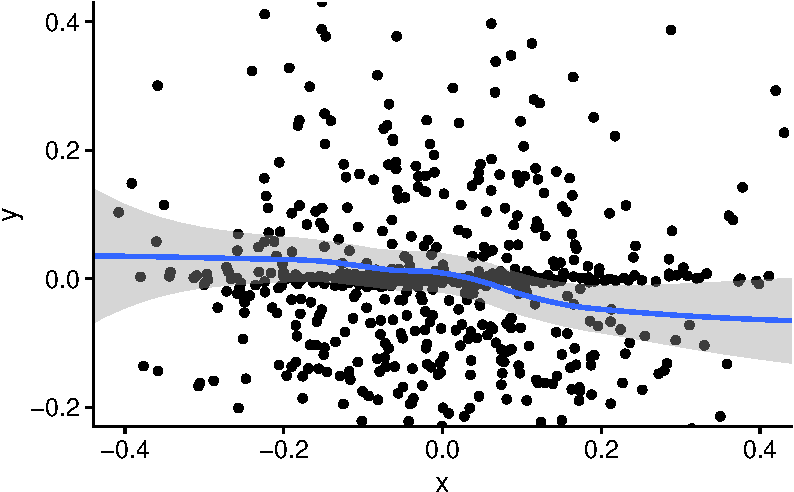
\includegraphics{IV_files/figure-pdf/unnamed-chunk-21-1.pdf}

\begin{Shaded}
\begin{Highlighting}[]
\CommentTok{\# (1)}
\NormalTok{mod\_conf\_probit }\OtherTok{\textless{}{-}} \FunctionTok{feglm}\NormalTok{(}
  \AttributeTok{fml =}\NormalTok{ any\_prio }\SpecialCharTok{\textasciitilde{}}
\NormalTok{    gdp\_g }\SpecialCharTok{+} 
\NormalTok{    gdp\_g\_l}
  \SpecialCharTok{+}\NormalTok{ gdp\_1979}
  \SpecialCharTok{+}\NormalTok{ polity2l }
  \SpecialCharTok{+}\NormalTok{ ethfrac }
  \SpecialCharTok{+}\NormalTok{ relfrac }
  \SpecialCharTok{+}\NormalTok{ oil }
  \SpecialCharTok{+}\NormalTok{ lmtnest }
  \SpecialCharTok{+}\NormalTok{ lpopl1 }
  \SpecialCharTok{+}\NormalTok{ year,}
  \AttributeTok{data =}\NormalTok{ rainconflict,}
  \AttributeTok{vcov =} \SpecialCharTok{\textasciitilde{}}\NormalTok{ ccode, }
  \AttributeTok{family =} \FunctionTok{binomial}\NormalTok{(}\AttributeTok{link =} \StringTok{"probit"}\NormalTok{)}
\NormalTok{) }

\FunctionTok{library}\NormalTok{(marginaleffects)}

\NormalTok{mod\_conf\_probit\_avge }\OtherTok{\textless{}{-}}\NormalTok{ mod\_conf\_probit }\SpecialCharTok{\%\textgreater{}\%} 
  \FunctionTok{avg\_slopes}\NormalTok{() }

\CommentTok{\# (2)}
\NormalTok{(}
\NormalTok{mod\_conf\_ols }\OtherTok{\textless{}{-}} \FunctionTok{feols}\NormalTok{(}
  \AttributeTok{fml =}\NormalTok{ any\_prio }\SpecialCharTok{\textasciitilde{}}
\NormalTok{    gdp\_g }\SpecialCharTok{+} 
\NormalTok{    gdp\_g\_l}
  \SpecialCharTok{+}\NormalTok{ gdp\_1979}
  \SpecialCharTok{+}\NormalTok{ polity2l }
  \SpecialCharTok{+}\NormalTok{ ethfrac }
  \SpecialCharTok{+}\NormalTok{ relfrac }
  \SpecialCharTok{+}\NormalTok{ oil }
  \SpecialCharTok{+}\NormalTok{ lmtnest }
  \SpecialCharTok{+}\NormalTok{ lpopl1 }
  \SpecialCharTok{+}\NormalTok{ year,}
  \AttributeTok{data =}\NormalTok{ rainconflict,}
  \AttributeTok{vcov =} \SpecialCharTok{\textasciitilde{}}\NormalTok{ ccode}
\NormalTok{) }
\NormalTok{)}
\end{Highlighting}
\end{Shaded}

\begin{verbatim}
OLS estimation, Dep. Var.: any_prio
Observations: 743
Standard-errors: Clustered (ccode) 
             Estimate Std. Error   t value Pr(>|t|)    
(Intercept) -5.381928  12.515620 -0.430017 0.669491    
gdp_g       -0.332716   0.263400 -1.263157 0.213846    
gdp_g_l     -0.084997   0.240857 -0.352894 0.726021    
gdp_1979    -0.040662   0.049894 -0.814961 0.419921    
polity2l     0.000642   0.004515  0.142164 0.887664    
ethfrac      0.230431   0.271367  0.849151 0.400851    
relfrac     -0.237764   0.241595 -0.984144 0.330961    
oil          0.045297   0.211526  0.214144 0.831523    
lmtnest      0.075811   0.039371  1.925548 0.061291 .  
lpopl1       0.068052   0.051102  1.331675 0.190506    
year         0.002483   0.006366  0.390106 0.698528    
---
Signif. codes:  0 '***' 0.001 '**' 0.01 '*' 0.05 '.' 0.1 ' ' 1
RMSE: 0.414086   Adj. R2: 0.113662
\end{verbatim}

\begin{Shaded}
\begin{Highlighting}[]
\CommentTok{\# (3)}
\FunctionTok{feols}\NormalTok{(}
  \AttributeTok{fml =}\NormalTok{ any\_prio }\SpecialCharTok{\textasciitilde{}} \SpecialCharTok{{-}}\DecValTok{1}
  \SpecialCharTok{+}\NormalTok{  gdp\_g }\SpecialCharTok{+} 
\NormalTok{    gdp\_g\_l}
  \SpecialCharTok{+}\NormalTok{ gdp\_1979}
  \SpecialCharTok{+}\NormalTok{ polity2l }
  \SpecialCharTok{+}\NormalTok{ ethfrac }
  \SpecialCharTok{+}\NormalTok{ relfrac }
  \SpecialCharTok{+}\NormalTok{ oil }
  \SpecialCharTok{+}\NormalTok{ lmtnest }
  \SpecialCharTok{+}\NormalTok{ lpopl1 }
  \SpecialCharTok{+} \FunctionTok{i}\NormalTok{(ccode, year),}
  \AttributeTok{data =}\NormalTok{ rainconflict,}
  \AttributeTok{vcov =} \SpecialCharTok{\textasciitilde{}}\NormalTok{ ccode}
\NormalTok{) }\SpecialCharTok{\%\textgreater{}\%} 
  \FunctionTok{summary}\NormalTok{(}\AttributeTok{n =} \DecValTok{10}\NormalTok{)}
\end{Highlighting}
\end{Shaded}

\begin{verbatim}
OLS estimation, Dep. Var.: any_prio
Observations: 743
Standard-errors: Clustered (ccode) 
                 Estimate Std. Error   t value Pr(>|t|)    
gdp_g           -0.387996   0.208988 -1.856550 0.070751 .  
gdp_g_l         -0.086461   0.212442 -0.406986 0.686188    
gdp_1979         2.287334   9.856030  0.232075 0.817663    
polity2l        -0.001355   0.004148 -0.326768 0.745547    
ethfrac         43.124761  50.926744  0.846800 0.402145    
relfrac         39.765573  63.751088  0.623763 0.536324    
oil              0.006172   0.086301  0.071511 0.943347    
lmtnest         -3.835094   7.462461 -0.513918 0.610137    
lpopl1           1.211169   0.671842  1.802760 0.078964 .  
ccode::404:year -0.033077   0.019564 -1.690721 0.098669 .  
... 40 coefficients remaining
---
Signif. codes:  0 '***' 0.001 '**' 0.01 '*' 0.05 '.' 0.1 ' ' 1
RMSE: 0.294151   Adj. R2: 0.526933
\end{verbatim}

\begin{Shaded}
\begin{Highlighting}[]
\CommentTok{\# (4)}
\FunctionTok{feols}\NormalTok{(}
  \AttributeTok{fml =}\NormalTok{ any\_prio }\SpecialCharTok{\textasciitilde{}} \SpecialCharTok{{-}}\DecValTok{1}
  \SpecialCharTok{+}\NormalTok{  gdp\_g }
  \SpecialCharTok{+}\NormalTok{  gdp\_g\_l}
  \SpecialCharTok{+} \FunctionTok{i}\NormalTok{(ccode, year)}
  \SpecialCharTok{|}\NormalTok{ ccode,}
  \AttributeTok{data =}\NormalTok{ rainconflict,}
  \AttributeTok{vcov =} \SpecialCharTok{\textasciitilde{}}\NormalTok{ ccode}
\NormalTok{) }\SpecialCharTok{\%\textgreater{}\%} 
  \FunctionTok{summary}\NormalTok{(}\AttributeTok{n =} \DecValTok{10}\NormalTok{)}
\end{Highlighting}
\end{Shaded}

\begin{verbatim}
OLS estimation, Dep. Var.: any_prio
Observations: 743
Fixed-effects: ccode: 41
Standard-errors: Clustered (ccode) 
                 Estimate Std. Error    t value  Pr(>|t|)    
gdp_g           -0.210909   0.156046  -1.351587   0.18410    
gdp_g_l          0.066801   0.158944   0.420279   0.67653    
ccode::404:year  0.028626   0.001635  17.510274 < 2.2e-16 ***
ccode::420:year -0.015243   0.000745 -20.452968 < 2.2e-16 ***
ccode::432:year  0.007220   0.000373  19.349039 < 2.2e-16 ***
ccode::433:year  0.059746   0.000225 265.584211 < 2.2e-16 ***
ccode::434:year  0.000449   0.000485   0.924683   0.36068    
ccode::435:year  0.000223   0.000544   0.410843   0.68338    
ccode::436:year  0.035483   0.000574  61.802750 < 2.2e-16 ***
ccode::437:year  0.000284   0.001085   0.261893   0.79475    
... 33 coefficients remaining
---
Signif. codes:  0 '***' 0.001 '**' 0.01 '*' 0.05 '.' 0.1 ' ' 1
RMSE: 0.239816     Adj. R2: 0.669782
                 Within R2: 0.370655
\end{verbatim}

\begin{Shaded}
\begin{Highlighting}[]
\DocumentationTok{\#\#\#\# IV models \#\#\#\#}

\CommentTok{\# (5)}
\FunctionTok{feols}\NormalTok{(}
  \AttributeTok{fml =}\NormalTok{ any\_prio }\SpecialCharTok{\textasciitilde{}}
  \SpecialCharTok{+}\NormalTok{ gdp\_1979}
  \SpecialCharTok{+}\NormalTok{ polity2l }
  \SpecialCharTok{+}\NormalTok{ ethfrac }
  \SpecialCharTok{+}\NormalTok{ relfrac }
  \SpecialCharTok{+}\NormalTok{ oil }
  \SpecialCharTok{+}\NormalTok{ lmtnest }
  \SpecialCharTok{+}\NormalTok{ lpopl1 }
  \SpecialCharTok{+} \FunctionTok{i}\NormalTok{(ccode, year)}
  \SpecialCharTok{|}\NormalTok{ gdp\_g }\SpecialCharTok{+}\NormalTok{ gdp\_g\_l }\SpecialCharTok{\textasciitilde{}}\NormalTok{ GPCP\_g }\SpecialCharTok{+}\NormalTok{ GPCP\_g\_l, }
  \AttributeTok{data =}\NormalTok{ rainconflict,}
  \AttributeTok{vcov =} \SpecialCharTok{\textasciitilde{}}\NormalTok{ ccode}
\NormalTok{) }\SpecialCharTok{\%\textgreater{}\%} 
  \FunctionTok{summary}\NormalTok{(}\AttributeTok{n =} \DecValTok{10}\NormalTok{)}
\end{Highlighting}
\end{Shaded}

\begin{verbatim}
TSLS estimation - Dep. Var.: any_prio
                  Endo.    : gdp_g, gdp_g_l
                  Instr.   : GPCP_g, GPCP_g_l
Second stage: Dep. Var.: any_prio
Observations: 743
Standard-errors: Clustered (ccode) 
               Estimate Std. Error   t value Pr(>|t|)    
(Intercept) -153.157460  60.518562 -2.530752 0.015419 *  
fit_gdp_g     -1.343217   1.462578 -0.918390 0.363920    
fit_gdp_g_l   -2.714015   1.036990 -2.617205 0.012453 *  
gdp_1979       9.446193  11.069500  0.853353 0.398545    
polity2l      -0.005806   0.004843 -1.198875 0.237631    
ethfrac       83.847478  47.883805  1.751061 0.087601 .  
relfrac       95.038889  64.178048  1.480863 0.146478    
oil           -0.058890   0.066111 -0.890779 0.378375    
lmtnest        2.159746   7.025786  0.307403 0.760132    
lpopl1        -0.336984   0.868944 -0.387809 0.700213    
... 41 coefficients remaining
---
Signif. codes:  0 '***' 0.001 '**' 0.01 '*' 0.05 '.' 0.1 ' ' 1
RMSE: 0.346685   Adj. R2: 0.342806
F-test (1st stage), gdp_g  : stat = 7.81825, p = 4.389e-4, on 2 and 692 DoF.
F-test (1st stage), gdp_g_l: stat = 5.56598, p = 0.003999, on 2 and 692 DoF.
                 Wu-Hausman: stat = 2.56365, p = 0.077756, on 2 and 690 DoF.
\end{verbatim}

\begin{Shaded}
\begin{Highlighting}[]
\CommentTok{\# (6)}
\FunctionTok{feols}\NormalTok{(}
  \AttributeTok{fml =}\NormalTok{ any\_prio }\SpecialCharTok{\textasciitilde{}} 
  \SpecialCharTok{+} \FunctionTok{i}\NormalTok{(ccode, year)}
  \SpecialCharTok{|}\NormalTok{ ccode}
  \SpecialCharTok{|}\NormalTok{ gdp\_g }\SpecialCharTok{+}\NormalTok{ gdp\_g\_l }\SpecialCharTok{\textasciitilde{}}\NormalTok{ GPCP\_g }\SpecialCharTok{+}\NormalTok{ GPCP\_g\_l, }
  \AttributeTok{data =}\NormalTok{ rainconflict,}
  \AttributeTok{vcov =} \SpecialCharTok{\textasciitilde{}}\NormalTok{ ccode}
\NormalTok{) }\SpecialCharTok{\%\textgreater{}\%} 
  \FunctionTok{summary}\NormalTok{(}\AttributeTok{n =} \DecValTok{10}\NormalTok{)}
\end{Highlighting}
\end{Shaded}

\begin{verbatim}
TSLS estimation - Dep. Var.: any_prio
                  Endo.    : gdp_g, gdp_g_l
                  Instr.   : GPCP_g, GPCP_g_l
Second stage: Dep. Var.: any_prio
Observations: 743
Fixed-effects: ccode: 41
Standard-errors: Clustered (ccode) 
                 Estimate Std. Error   t value   Pr(>|t|)    
fit_gdp_g       -1.131763   1.362254 -0.830802 4.1102e-01    
fit_gdp_g_l     -2.546473   1.070475 -2.378825 2.2230e-02 *  
ccode::404:year  0.006632   0.013806  0.480372 6.3358e-01    
ccode::420:year -0.005215   0.006294 -0.828648 4.1222e-01    
ccode::432:year  0.012689   0.003059  4.148704 1.6945e-04 ***
ccode::433:year  0.063170   0.001807 34.960834  < 2.2e-16 ***
ccode::434:year  0.006202   0.004195  1.478344 1.4715e-01    
ccode::435:year  0.008547   0.004353  1.963488 5.6568e-02 .  
ccode::436:year  0.043387   0.004817  9.007338 3.5998e-11 ***
ccode::437:year  0.017506   0.008435  2.075379 4.4425e-02 *  
... 33 coefficients remaining
---
Signif. codes:  0 '***' 0.001 '**' 0.01 '*' 0.05 '.' 0.1 ' ' 1
RMSE: 0.302046     Adj. R2: 0.476172
                 Within R2: 0.001663
F-test (1st stage), gdp_g  : stat = 6.67399, p = 0.001345, on 2 and 699 DoF.
F-test (1st stage), gdp_g_l: stat = 5.70442, p = 0.003488, on 2 and 699 DoF.
                 Wu-Hausman: stat = 3.14562, p = 0.043689, on 2 and 657 DoF.
\end{verbatim}

\begin{Shaded}
\begin{Highlighting}[]
\CommentTok{\# (7)}
\FunctionTok{feols}\NormalTok{(}
  \AttributeTok{fml =}\NormalTok{ war\_prio }\SpecialCharTok{\textasciitilde{}} 
    \SpecialCharTok{+} \FunctionTok{i}\NormalTok{(ccode, year)}
  \SpecialCharTok{|}\NormalTok{ ccode}
  \SpecialCharTok{|}\NormalTok{ gdp\_g }\SpecialCharTok{+}\NormalTok{ gdp\_g\_l }\SpecialCharTok{\textasciitilde{}}\NormalTok{ GPCP\_g }\SpecialCharTok{+}\NormalTok{ GPCP\_g\_l, }
  \AttributeTok{data =}\NormalTok{ rainconflict,}
  \AttributeTok{vcov =} \SpecialCharTok{\textasciitilde{}}\NormalTok{ ccode}
\NormalTok{) }\SpecialCharTok{\%\textgreater{}\%} 
  \FunctionTok{summary}\NormalTok{(}\AttributeTok{n =} \DecValTok{10}\NormalTok{)}
\end{Highlighting}
\end{Shaded}

\begin{verbatim}
TSLS estimation - Dep. Var.: war_prio
                  Endo.    : gdp_g, gdp_g_l
                  Instr.   : GPCP_g, GPCP_g_l
Second stage: Dep. Var.: war_prio
Observations: 743
Fixed-effects: ccode: 41
Standard-errors: Clustered (ccode) 
                 Estimate Std. Error   t value  Pr(>|t|)    
fit_gdp_g       -1.479970   0.800386 -1.849071  0.071848 .  
fit_gdp_g_l     -0.768785   0.678533 -1.133010  0.263956    
ccode::404:year -0.001514   0.007526 -0.201188  0.841571    
ccode::420:year  0.007088   0.003431  2.066077  0.045340 *  
ccode::432:year  0.003375   0.001670  2.020730  0.050037 .  
ccode::433:year  0.015992   0.000992 16.119071 < 2.2e-16 ***
ccode::434:year  0.004765   0.002306  2.065964  0.045351 *  
ccode::435:year  0.004698   0.002393  1.963229  0.056599 .  
ccode::436:year  0.005405   0.002624  2.059408  0.046005 *  
ccode::437:year  0.008802   0.004699  1.872980  0.068392 .  
... 33 coefficients remaining
---
Signif. codes:  0 '***' 0.001 '**' 0.01 '*' 0.05 '.' 0.1 ' ' 1
RMSE: 0.228949     Adj. R2: 0.575516
                 Within R2: 0.229726
F-test (1st stage), gdp_g  : stat = 6.67399, p = 0.001345, on 2 and 699 DoF.
F-test (1st stage), gdp_g_l: stat = 5.70442, p = 0.003488, on 2 and 699 DoF.
                 Wu-Hausman: stat = 1.46546, p = 0.231725, on 2 and 657 DoF.
\end{verbatim}

\begin{Shaded}
\begin{Highlighting}[]
\FunctionTok{library}\NormalTok{(modelsummary)}

\FunctionTok{modelsummary}\NormalTok{(}
  \AttributeTok{models =} \FunctionTok{list}\NormalTok{(}
\NormalTok{    mod\_conf\_probit\_avge, }
\NormalTok{    mod\_conf\_ols}
\NormalTok{    )}
\NormalTok{  )}
\end{Highlighting}
\end{Shaded}

\begin{table}
\centering
\begin{tblr}[         %% tabularray outer open
]                     %% tabularray outer close
{                     %% tabularray inner open
colspec={Q[]Q[]Q[]},
column{1}={halign=l,},
column{2}={halign=c,},
column{3}={halign=c,},
hline{24}={1,2,3}{solid, 0.05em, black},
}                     %% tabularray inner close
\toprule
& (1) & (2) \\ \midrule %% TinyTableHeader
ethfrac     & \num{0.220}   & \num{0.230}    \\
& (\num{0.242}) & (\num{0.271})  \\
gdp\_1979  & \num{-0.063}  & \num{-0.041}   \\
& (\num{0.058}) & (\num{0.050})  \\
gdp\_g     & \num{-0.350}  & \num{-0.333}   \\
& (\num{0.301}) & (\num{0.263})  \\
gdp\_g\_l & \num{-0.127}  & \num{-0.085}   \\
& (\num{0.251}) & (\num{0.241})  \\
lmtnest     & \num{0.072}   & \num{0.076}    \\
& (\num{0.036}) & (\num{0.039})  \\
lpopl1      & \num{0.074}   & \num{0.068}    \\
& (\num{0.049}) & (\num{0.051})  \\
oil         & \num{0.015}   & \num{0.045}    \\
& (\num{0.210}) & (\num{0.212})  \\
polity2l    & \num{0.001}   & \num{0.001}    \\
& (\num{0.005}) & (\num{0.005})  \\
relfrac     & \num{-0.271}  & \num{-0.238}   \\
& (\num{0.241}) & (\num{0.242})  \\
year        & \num{0.003}   & \num{0.002}    \\
& (\num{0.006}) & (\num{0.006})  \\
(Intercept) &                & \num{-5.382}   \\
&                & (\num{12.516}) \\
Num.Obs.    & \num{743}     & \num{743}      \\
R2          & \num{0.122}   & \num{0.126}    \\
R2 Adj.     & \num{0.099}   & \num{0.114}    \\
AIC         & \num{779.8}   & \num{820.4}    \\
BIC         & \num{830.6}   & \num{871.1}    \\
RMSE        & \num{0.42}    & \num{0.41}     \\
Std.Errors  &                & by: ccode       \\
\bottomrule
\end{tblr}
\end{table}

\bookmarksetup{startatroot}

\chapter{Difference-in-Differences}\label{difference-in-differences}

Der Difference-in-Differences (DID) Ansatz erlaubt die Schätzung
kausaler Effekte in quasi-experimentellen Forschungsdesigns, in denen
Boebachtungen für Kontroll- und Behandlungsgruppe zu mindestens zwei
Zeitpunkten vorliegen und die Behandlung zwischen diesen Zeitpunkten
stattfindet: Wir beobachten sowohl die Kontroll- als auch die
Behandlungsgruppe vor und nachdem die Behandlung erfolgt ist. Die
Motivation für die Anwendung des DID-Ansatzes liegt in der Fähigkeit,
typische Risiken einer Verzerrungen zu umgehen, die bei einfachen
Vorher-Nachher-Vergleichen oder reinen Querschnittsvergleichen auftreten
können. Die Kernidee ist eine Schätzung des ATT durch einen Vergleich
durchschnittlicher Differenzen der Outcome-Variable beider Gruppen
zwischen den Perdioden vor und nach der Intervention.
Abbildung~\ref{fig-CDDID} zeigt ein kausales Diagramm für ein
Forschungsdesign, in dem DID den ATT identifizieren kann.

\begin{figure}[t]

\centering{

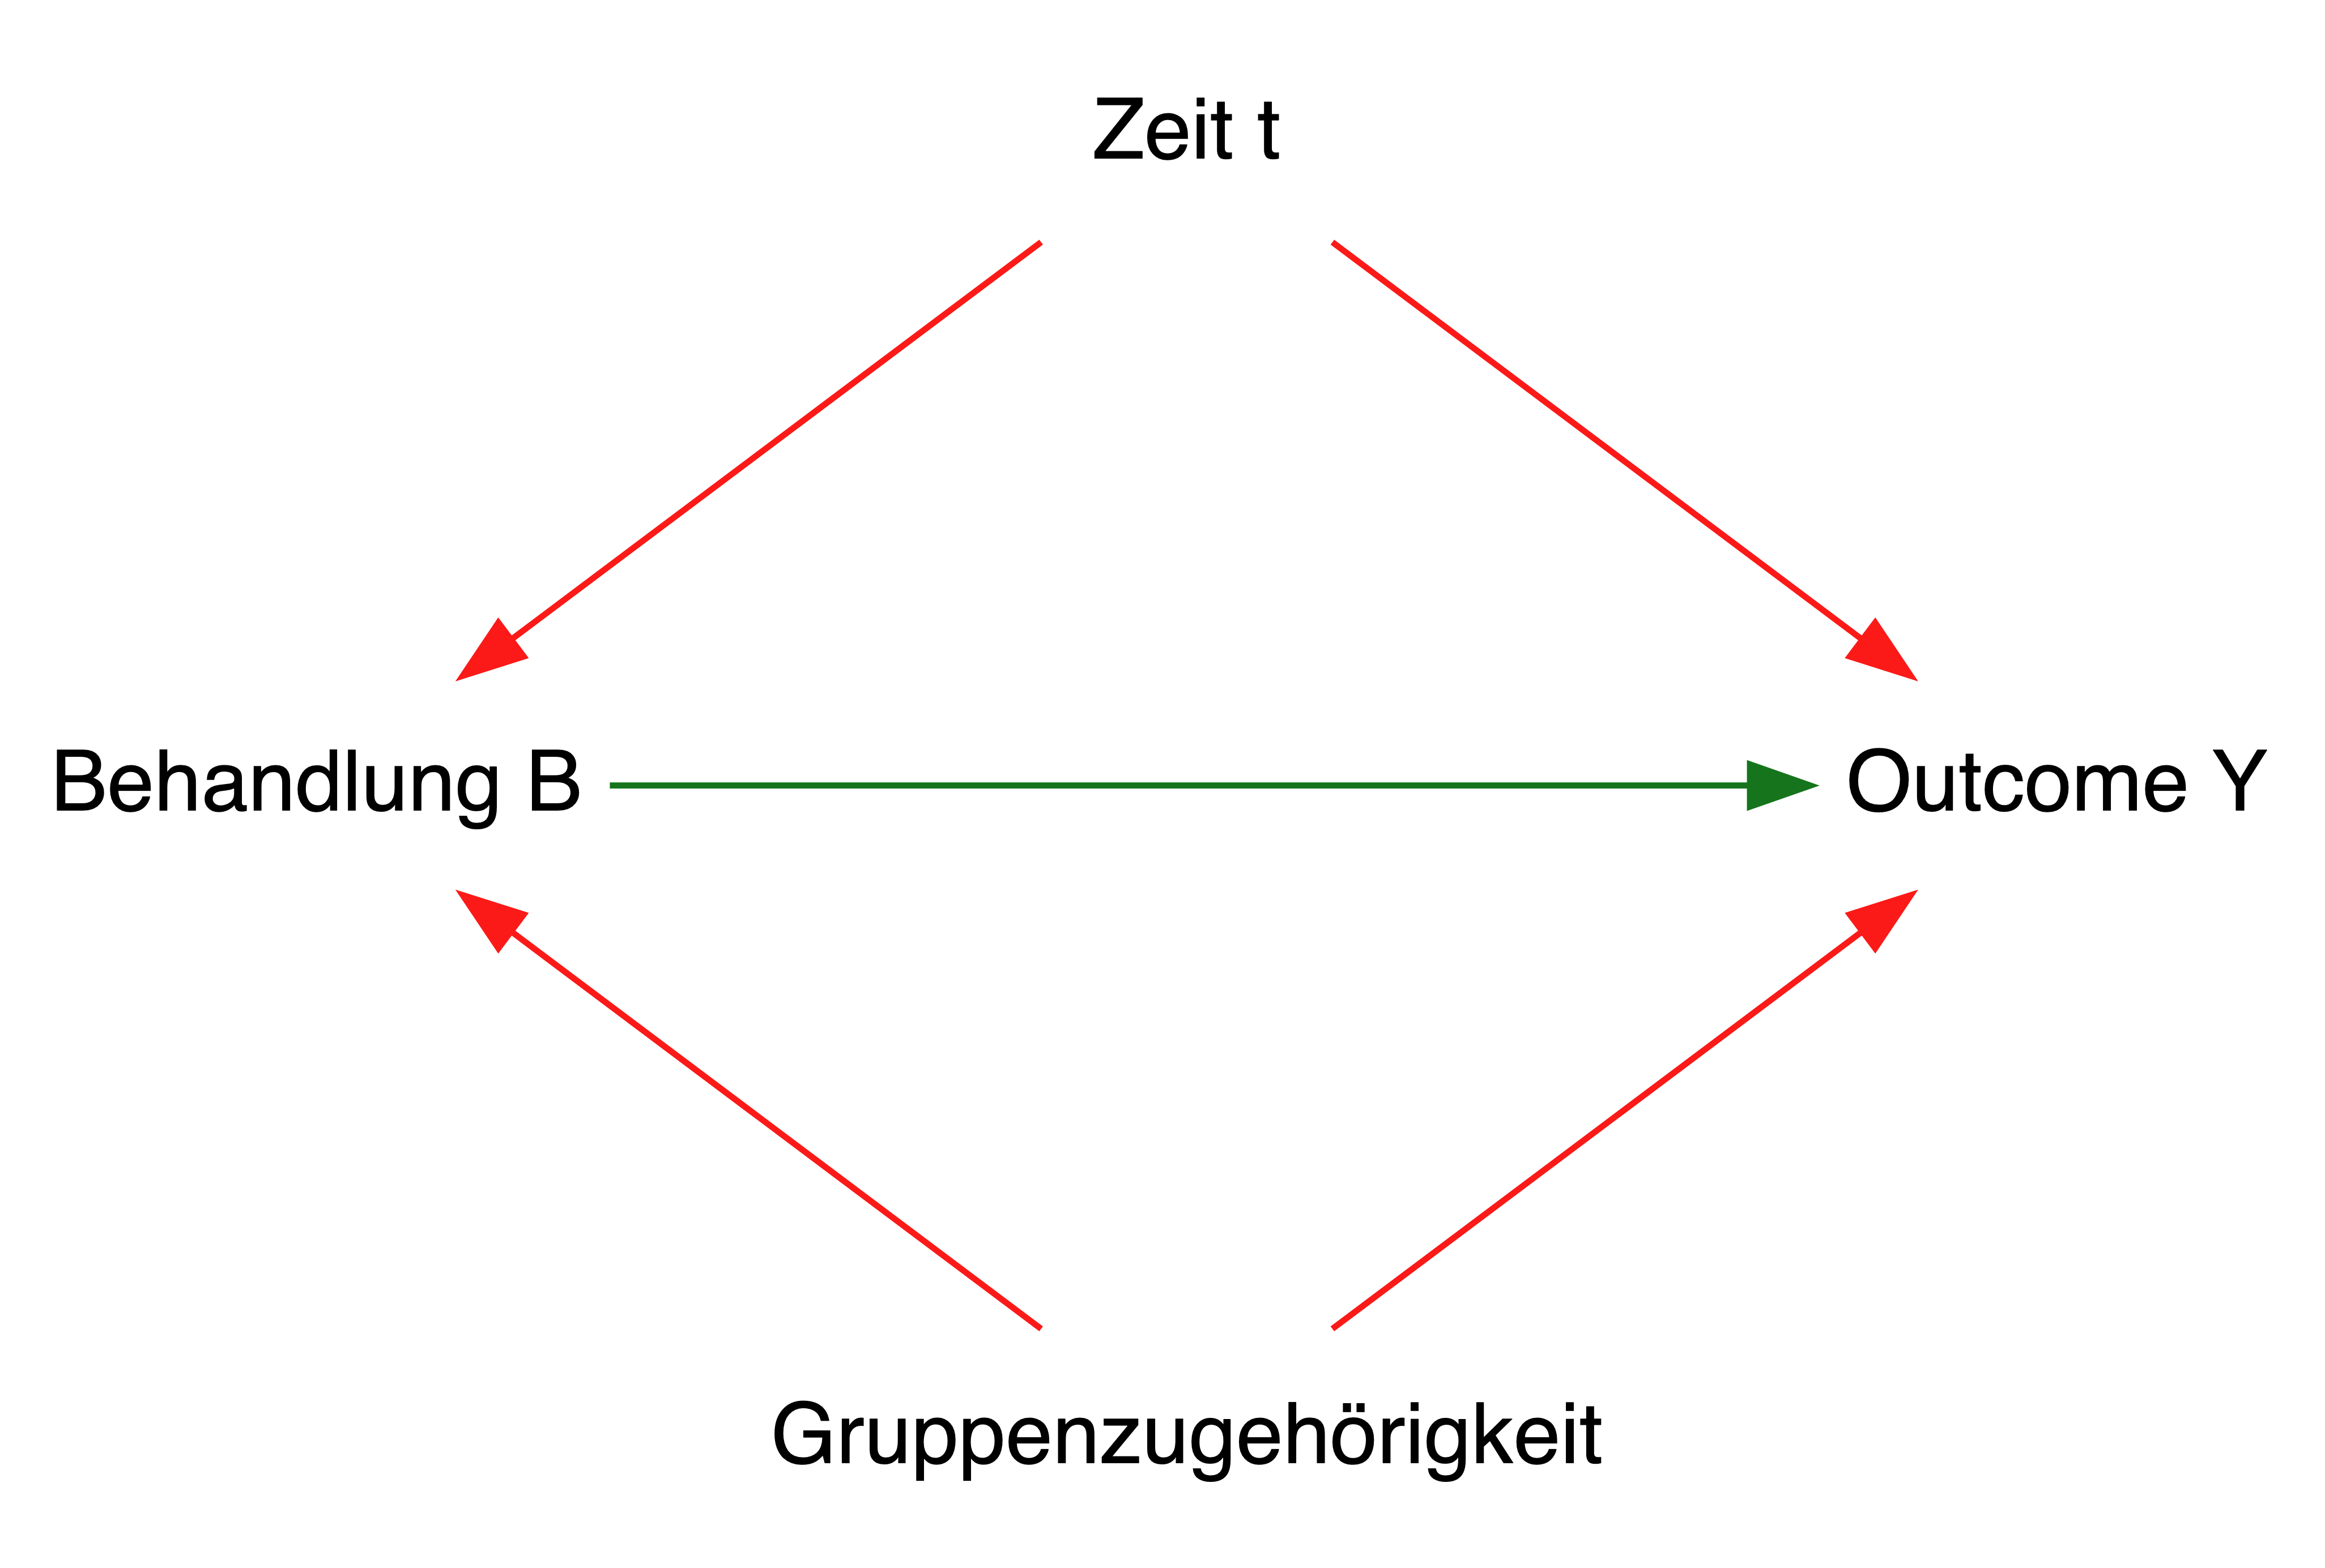
\includegraphics[width=5in,height=3in]{DiD_files/figure-latex/dot-figure-1.png}

}

\caption{\label{fig-CDDID}Kausales Diagramm für DID}

\end{figure}%

Abbildung~\ref{fig-CDDID} illustriert Confounding bei der Bestimmung des
Behandlungseffekts durch Backdoors in der Zeit \(t\) und der
Gruppenzugehörigkeit:

\begin{itemize}
\item
  \textbf{Zeit}: Der Behandlungszustand der behandelten Gruppe ändert
  sich durch die Intervention zwischen der Vor- und der
  Nachbehandlungsperiode. Die Outcome-Variable \(Y\) ändert sich für
  beide Gruppen über die Zeit hinweg.
\item
  \textbf{Gruppenzugehörigkeit}: Die Gruppenzugehörigkeit legt fest, ob
  eine Behandlung erfolgt. Systematische Unterschiede zwischen
  Behandlungs- und Kontrollgruppe wirken sich auf die Outcome-Variable
  \(Y\) aus.
\end{itemize}

In einem DID-Ansatz ermöglicht die Beobachtung von Kontroll- und
Behandlungsgruppen jeweils \emph{bevor und nach} einer Intervention das
Herausrechnen von systematischen Unterschieden zwischen Behandlungs- und
Kontrollgruppe und von Zeiteffekten, sodass die Backdoors durch
Gruppenzugehörigkeit und Zeit geschlossen. Die Schätzung eines
durchschnittlichen Behandlungseffekts erfolgt hierbei unter der Annahme,
dass die Outcome-Variable beider Gruppen \emph{ohne die Intervention}
einen hinreichend ähnlichen Verlauf aufweisen würde und damit die
Kontrollgruppe ein plausibles Counterfactual für die Behandlungsgruppe
darstellt.

\section{Einordnung im Potential Outcomes
Framework}\label{einordnung-im-potential-outcomes-framework}

Im Potential Outcomes Framework nehmen wir an, dass jede Einheit \(i\)
in Abhänigkeit ihres Behandlungsstatus zwei potentielle Ergebnisse hat.
Wir unterscheiden zwischen Beobachtungen in Behandlungs- und
Kontrollgruppe:

\begin{itemize}
\tightlist
\item
  \(Y_{i,B}(1)\): \(Y\) für Einheit \(i\) in der Behandlungsgruppe, wenn
  diese behandelt wird.
\item
  \(Y_{i,B}(0)\): \(Y\) für Einheit \(i\) in der Behandlungsgruppe, wenn
  diese \emph{nicht} behandelt wird.
\item
  \(Y_{i,K}(1)\): \(Y\) für Einheit \(i\) in der Kontrollgruppe, wenn
  diese behandelt wird.
\item
  \(Y_{i,K}(0)\): \(Y\) für Einheit \(i\) in der Kontrollgruppe, wenn
  diese \emph{nicht} behandelt wird.
\end{itemize}

In einem DID-Forschungsdesign hängen tatsächliche und potentielle
Outcomes von der Zeit \(t\) ab: Die Behandlungsgruppe wird zwischen den
Zeitpunkten \(t = 0\) und \(t = 1\) behandelt, während die
Kontrollgruppe unbehandelt bleibt. Für die Identifizierung des
Behandlungseffekts wird unterstellt, dass \(Y\) sich zwischen \(t=0\)
und \(t=1\) in der Behandlungsgruppe \emph{ohne eine Behandlung} (im
Erwartungswert) mit demselben Trend entwickelt hätte, mit dem sich die
Kontrollgruppe tatsächlich entwickelt hat (parallele Trends). Die
Gültigkeit paralleler Trends ist entscheidend für die Validität der
DID-Methode, da so sicherstellt ist, dass die beobachteten Unterschiede
in den Ergebnissen auf die Behandlung zurückzuführen sind und nicht auf
andere zeitgleich auftretende Faktoren. Der Behandlungseffekt kann dann
als eine \emph{Differenz von Differenzen} geschrieben werden:

\begin{align}
  \begin{split}
    \beta_\textup{DID} =& \, \bigg({\color{red}\textup{E}\big[Y_B(1)\vert t=1\big] - \textup{E}\big[Y_B(0)\vert t=0\big]} \bigg)\\
  -&\, \bigg({\color{blue}\textup{E}\big[Y_K(0)\vert t=1\big] -  \textup{E}\big[Y_K(0)\vert t=0\big]} \bigg)
  \end{split}\label{eq:DID-ATT1}
\end{align}

Der Effekt \(\beta_\textup{DID}\) ist ein ATT, der über das Schließen
der Backdoor in der Zeit (rote und blaue Differenzen der Erwartungswerte
zwischen \(t=0\) und \(t=1\)) sowie der Backdoor in der
Gruppenzugehörigkeit (Differenz der Erwartungswert-Differenzen)
identifiziert wird.

Eine Null-Ergänzung von \eqref{eq:DID-ATT1} mit
\({\color{blue}\textup{E}\big[Y_K(0)\vert t=1\big] -  \textup{E}\big[Y_K(0)\vert t=1\big]}\)
zeigt die Wichtigkeit der Gültigkeit paralleler Trends:

\begin{align*}
    \beta_\textup{DID} =& \, \bigg({\color{red}\textup{E}\big[Y_B(1)\vert t=1\big] - \textup{E}\big[Y_B(0)\vert t=0\big]} \bigg)
  - \bigg({\color{blue}\textup{E}\big[Y_K(0)\vert t=1\big] -  \textup{E}\big[Y_K(0)\vert t=0\big]} \bigg)\\ + &\,
{\color{blue}\textup{E}\big[Y_K(0)\vert t=1\big] -  \textup{E}\big[Y_K(0)\vert t=1\big]}\\
    \\
    =&\, \underbrace{{\color{red}\textup{E}\big[Y_B(1)\vert t=1\big]} - {\color{blue}\textup{E}\big[Y_B(1)\vert t=1\big]}}_{=\textup{ATT}}\\
    +&\, \underbrace{\bigg({\color{red}\textup{E}\big[Y_B(0)\vert t=1\big] - \textup{E}\big[Y_B(0)\vert t=0\big]} \bigg) - \bigg({\color{blue}\textup{E}\big[Y_K(0)\vert t=1\big] -  \textup{E}\big[Y_K(0)\vert t=0\big]} \bigg)}_{ = \textup{Verzerrung durch nicht-parallele Trends}}
\end{align*}

Diese Zerlegung zeigt, dass der ATT nur bei parallelen Trends
identifziert werden kann, d.h. wir benötigen

\begin{align*}
{\color{red}\textup{E}\big[Y_B(0)\vert t=1\big] - \textup{E}\big[Y_B(0)\vert t=0\big]} = {\color{blue}\textup{E}\big[Y_K(0)\vert t=1\big] -  \textup{E}\big[Y_K(0)\vert t=0\big]}.
\end{align*}

Beachte, dass \({\color{red}\textup{E}\big[Y_B(0)\vert t=1\big]}\) der
Erwartungswert des potentiellen Outcomes einer unbehandelten
Behandlungsgruppe in \(t=1\) ist. Somit kann die Verzerrung durch
nicht-parallele Trends nicht empirisch überprüft werden und muss
ausschließlich durch das Forschungsdesign gewährleistet sein. In
Anwendungen kann die Plausibilität der Annahme graphisch anhand
geschätzter Trends in der Outcome-Variable oder durch Placebo-Tests
untersucht werden.

\textbf{Annahmen für DID}

\begin{enumerate}
\def\labelenumi{\arabic{enumi}.}
\item
  \textbf{Parallele Trends}: Die Trends in der Outcome Variable \(Y\) in
  Behandlungs- und Kontrollgruppe würden bis einschließlich \(t=1\)
  parallel verlaufen, wenn es keine Behandlung gäbe. Diese Annahme ist
  Voraussetzung dafür, dass Veränderungen im Outcome \(Y\) für die
  Behandlungsgruppe, die sich von \(Y\) für die Kontrollgruppe
  unterscheidet, auschließlich dem Effekt der Behandlung zugeschrieben
  werden kann.
\item
  \textbf{Keine Interferenz und konsistente Behandlung (SUTVA)}:

  \begin{itemize}
  \item
    \emph{Keine Interferenz}: Die Behandlung eines Individums hat keinen
    Einfluss auf das potentielle Outcome anderer Individuen, unabhängig
    von der Gruppenzugehörigkeit.
  \item
    \emph{Konsistete Behandlung}: Es gibt keine Variation in der
    Intensität oder Art der Behandlung innerhalb der Behandlungsgruppe.
  \end{itemize}
\end{enumerate}

\section{Schätzung des ATT mit DID}\label{schuxe4tzung-des-att-mit-did}

Für die Schätzung von \(\beta_\text{DID}\) ersetzen wir die
Erwartungswerte in \eqref{eq:DID-ATT1} durch ihre Stichprobenmomente.
Dies liefert den Schätzer

\begin{align}
  \widehat{\beta}_\textup{DID} = \bigg({\color{red}\overline{Y_B(1)\vert t=1} - \overline{Y_B(0)\vert t=0}} \bigg) -  \bigg({\color{blue}\overline{Y_K(0)\vert t=1} - \overline{Y_K(0)\vert t=0}}\bigg). \label{eq:DIDMOMENTS}
\end{align}

Die Implementierung von DID-Schätzern erfolgt meist anhand linearer
Regression. Das Modell für zwei Zeitperioden ist

\begin{align}
  Y_{i,\,t} = \alpha + \beta_1 B_i + \beta_2 Z_t + \beta_3 (B_i \times Z_t) + \epsilon_{i,\,t}, \quad t\in\{0,1\}, \label{eq:DIDREG}
\end{align}

wobei \(\beta_3\) der interessierende Behandlungseffekt ist. Der
Regressor \(B_i \times Z_t\) ist die Interaktion zwischen der
Behandlungsgruppenzugehörigkeit \(B_i\) und einem Indikator für den
Zeitpunkt \emph{nach} der Intervention, \(Z_i = \mathbb{I}_{\{t=1\}}\).
Beachte, dass wir in Modell \eqref{eq:DIDREG} für Zeiteffekte und
Gruppenzugehörig kontrollieren und damit die sich durch das
Forschungsdesign ergebenden Backdoors (vgl. Abbildung~\ref{fig-CDDID})
schließen.

Es ist \(\widehat\beta_3 = \widehat{\beta}_\text{DID}\), d.h. der
KQ-Schätzer von \(\beta_3\) ist der DID-Schätzer des ATT und numerisch
äquivalent zu \eqref{eq:DIDMOMENTS}. Die Berechnung von
\(\widehat\beta_\text{DID}\) anhand von Modell \eqref{eq:DIDREG} ist
praktisch, da wir so Inferenzstatistiken mit etablierten R-Funktionen
wie \texttt{summary()} und \texttt{lmtest::coeftest()} wie gewohnt
berechnen können.

In empirischen Anwendungen stehen oft Datensätze mit mehreren Gruppen
und mehr als zwei Beobachtungsperioden zur Verfügung. Beachte, dass das
Modell \eqref{eq:DIDREG} ein Spezialfall des allgemeinen
Forschungsdesigns mit \(t=1,\dots,T\) für \(T\geq2\)
Beobachtungsperioden und mehr als zwei Gruppen (mehrere Kontroll- und
Behandlungsgruppen) ist. Eine dann häufig genutzte Modellspezifikation
für die Schätzung des ATT mit DID ist eine Panel-Regression mit
\emph{Two-way Fixed Effects},

\begin{align}
  Y_{i,\,t} =  \theta_i + \eta_t + \beta_\text{DID}^\text{TWFE} D_{i,\, t} + \epsilon_{i,\,t}, \quad t = 1,\dots,T, \label{eq:TWFEDIDREG}
\end{align}

wobei \(\theta_i\) und \(\eta_t\) Dummy-Variablen für Gruppen und
Zeitperioden sind und \(D_{i,\, t}\) der Behandlungsindikator ist.
Dieses lineare Paneldaten-Modell kann komfortabel mit dem R-Paket
\texttt{fixest} (s. \texttt{fixtest::feols()}) implementiert werden. Bei
mehreren Gruppen sollten cluster-robuste Standardfehler auf
Gruppen-Ebene verwendet werden.

In Modell \eqref{eq:TWFEDIDREG} indentifiziert
\(\beta_\text{DID}^\text{TWFE}\) den ATE, sofern die Annahmen 1
(parallele Trends) und 2 (SUTVA) gelten. Damit die Annahme paralleler
Trends gewährleistet ist, dürfen keine heterogenen Behandlungseffekte
vorliegen, d.h. die Behandlungseffekte

\begin{itemize}
\tightlist
\item
  variieren nicht zwischen verschiedenen Gruppen
\item
  sind unabhängig vom Zeitpunkt der Behandlung (relevant bei
  unterschiedlichen Behandlungszeitpunkten)
\item
  entwickeln sich nicht dynamisch über die Zeit\footnote{Siehe bspw.
    Goodman-Bacon (2021) für eine detaillierte Diskussion dieser
    Problematik.}
\end{itemize}

Der Umgang mit heterogenen Behandlungseffekten ist Gegenstand der
aktuellen ökonometrischen Forschung zu DID-Schätzern. Callaway und
Sant'Anna (2021) schlagen eine nicht-parametrische Schätzung von
gruppenspezifischen ATE zu veschiedenen Zeitpunkten vor, die zu einem
globalen ATT zusammengefasst werden können.\footnote{Die Methoden von
  Callaway und Sant'Anna (2021) sind im R-Paket \texttt{did}
  implementiert.}

\begin{tcolorbox}[enhanced jigsaw, bottomtitle=1mm, colbacktitle=quarto-callout-note-color!10!white, coltitle=black, arc=.35mm, title=\textcolor{quarto-callout-note-color}{\faInfo}\hspace{0.5em}{Key Facts zum einfachen DID-Schätzer}, titlerule=0mm, opacityback=0, breakable, bottomrule=.15mm, toprule=.15mm, opacitybacktitle=0.6, colframe=quarto-callout-note-color-frame, toptitle=1mm, rightrule=.15mm, leftrule=.75mm, left=2mm, colback=white]

\begin{itemize}
\item
  Im DID-Forschungsdesign kann der ATT durch einen Vergleich von
  \emph{Differenzen} in den Ergebnissen vor und nach einer Behandlung
  zwischen Behandlungs- und Kontrollgruppen identifiziert werden.
\item
  DID benötigt Beobachtungen einer Behandlungs- und einer Kontrollgruppe
  zu \emph{mindestens} zwei verschiedenen Zeitpunkten, wobei der
  Behandlung zwischen diesen Zeitpunkten erfolgt.
\item
  DID ist empfindlich gegenüber Verletzungen der Annahme, dass die
  zeitlichen Trends in der Outcome-Variable für die Behandlungs- und die
  Kontrollgruppen vor der Intervention parallel verlaufen.
\item
  DID-Schätzer können in linearen Interaktionsmodellen mit Fixed Effects
  für Zeitperioden und Gruppenzugehörigkeit implementiert werden. Der
  interessierenden Effekt sind die Koeffizienten von Interaktionstermem
  zwischen den Indikatoren für die Nachbehandlungsperioden und für die
  Zugehörigkeit zu einer Behandlungsgruppe.
\item
  In R können DID-Modelle mit \texttt{lm()} oder, in Fällen mit mehr als
  zwei Beobachtungsperioden, mit \texttt{fixest::feols()} geschätzt
  werden. In Forschungsdesigns mit mehreren Gruppen sollten
  cluster-robuste Standardfehler verwendet werden.
\end{itemize}

\end{tcolorbox}

\begin{center}\rule{0.5\linewidth}{0.5pt}\end{center}

Die nachfolgende interaktive Grafik illustriert die Schätzung des ATT
mit DID sowie die Verletzung der Annahme paralleler Trends anhand
simulierte Daten für mehrere Zeitperioden. Der verwendete DID-Schätzer
ist der KQ-Schätzer in Modell \eqref{eq:DIDREG}, d.h. wir betrachten ein
Forschungsdesign in dem zwei Zeitperioden für die Schätzung verwendet
werden, wobei die Behandlung zwischen diesen Perioden erfolgt.

\textbf{Interaktive Elemente der Visualisierung}

\begin{itemize}
\item
  Die Beobachtungen der Individuen zu 6 verschiedenen Zeitpunkten werden
  als Punkte dargestellt. Die Datenpunkte könn mit \emph{Zeige Daten}
  ein- und ausgeblendet werden.
\item
  Die geschätzten Trends beider Gruppen für den gesamten
  Beobachtungszeitraum und die Gruppenzugehörigkeit können mit
  \emph{Zeige Trends} ein- und ausgeblendet werden. Die Auswahl
  \emph{Parallele Trends} stellt sicher, dass beide Gruppen (mit
  Ausnahme des Behandlungseffekts in der Behandlungsgruppe) dem selben
  zeitlichen Trend folgen. Bei nicht-parallelen Trends folgt die
  Behandlungsgruppe einem positiven Trend mit größerer positiver
  Steigung als in der Kontrollgruppe.
\item
  Die Behandlung erfolgt zwischen der mit dem Slider \emph{Zeitpunkt}
  ausgewählten und der darauf folgenden Periode. Der tatsächliche
  Behandlungseffekt kann über den Slider \emph{Effekt} festgelegt
  werden.
\end{itemize}

\textbf{Anatomie der Schätzung des ATT bei \emph{parallelen} Trends}

\begin{itemize}
\item
  Wir illustrieren die Schätzen des ATT mit Formel
  \eqref{eq:DIDMOMENTS}. Kreise zeigen Mittelwerte für Kontroll- und
  Behandlungsgruppe \emph{vor} der Intervention. Dreiecke zeigen
  Mittelwerte \emph{nach} der Intervention.
\item
  Die gestrichelte rote Linie zeigt den (kontrafaktischen) Verlauf der
  Behandlungsgruppe \emph{ohne} Behandlung. Hierbei wird unterstellt,
  dass sich die Behandlungsgruppe mit demselben Trend \emph{wie die
  Kontrollgruppe entwickelt hätte} (blaue Linie).
\item
  Der geschätzte Behandlungseffekt wird als orangene vertikale Linie
  dargestellt. Dies ist die Differenz zwischen dem tatsächlichen
  post-Behandlungs-Mittelwert und dem kontrafaktischen Mittelwert der
  Behandlungsgruppe.
\end{itemize}

\textbf{Anatomie der Schätzung des ATT bei \emph{nicht-parallelen}
Trends}

\begin{itemize}
\item
  Für nicht-parallele Trends zeigt die Grafik den unterstellten
  kontrafaktischen Trend der Behandlungsgruppe als gestrichelte blaue
  linie. Der'' ``tatsächliche'' kontrafaktische Verlauf der
  Behandlungsgruppe wird als gestrichelte rote Linie dargestellt.
\item
  Aufgrund des steileren (positiven) Trends in der Behandlungsgruppe
  ergibt sich eine \emph{positive} Verzerrung von
  \(\color{orange}\widehat{\beta}_\text{DID}\). Diese Verzerrung wird
  durch die gestrichelte vertikale schwarze Linie kenntlich gemacht.

  \begin{itemize}
  \item
    Für \emph{positive} Behandlungseffekte wird der ATT
    \emph{überschätzt}: die Verzerrung entspricht der Überlagerung der
    gestrichelten schwarzen linie mit der orangenen Linie des
    geschätzten Effekts.
  \item
    Für \emph{negative} Behandlungseffekte wird der ATT unterschätzt:
    die Verzerrung entspricht der gestrichelten schwarzen Linie oberhalb
    der orangenen Linie des geschätzten Effekts.
  \end{itemize}
\end{itemize}

\begin{center}\rule{0.5\linewidth}{0.5pt}\end{center}

\section{Schätzung von DID-Forschungsdesigns mit
R}\label{schuxe4tzung-von-did-forschungsdesigns-mit-r}

Wir erläutern nachfolgend die Schätzung von DID-Designs mit zwei
Zeitperioden mit R und visualisieren die geschätzten Komponenten von
\(\widehat{\beta}_\text{DID}\) ähnlich wie in der interaktiven
Visualisierung. Hierzu erzeugen wir simulierte Daten gemäß der
Vorschrift

\begin{align*}
  Y_{i,t} &= 2 + 3 \cdot Z_t + 5 \cdot B_i + 4 \cdot (Z_t \cdot B_i) + \epsilon_{i,t}\\
  \epsilon_{i,t} &\sim N(0, 1)\\
  Z_t &= \mathbb{I}_{\{ t = 1 \}} \\
  B_i &= \mathbb{I}_{\{ i \in \textup{Behandlungsgruppe} \}},
\end{align*} wobei wir jeweils \(100\) Beobachtungen beider Gruppen zu
beiden Zeitpunkten generieren.

\begin{Shaded}
\begin{Highlighting}[]
\FunctionTok{library}\NormalTok{(tibble)}
\FunctionTok{library}\NormalTok{(dplyr)}

\CommentTok{\# Seed setzen}
\FunctionTok{set.seed}\NormalTok{(}\DecValTok{1234}\NormalTok{)}

\CommentTok{\# Anzahl der Beobachtungen (pro Gruppe u. Zeitpunkt)}
\NormalTok{n }\OtherTok{\textless{}{-}} \DecValTok{100}

\CommentTok{\# Daten simulieren}
\NormalTok{did\_data }\OtherTok{\textless{}{-}} \FunctionTok{tibble}\NormalTok{(}
  \AttributeTok{Z =} \FunctionTok{rep}\NormalTok{(}\FunctionTok{rep}\NormalTok{(}\FunctionTok{c}\NormalTok{(}\DecValTok{0}\NormalTok{, }\DecValTok{1}\NormalTok{), }\AttributeTok{each =}\NormalTok{ n), }\AttributeTok{times =} \DecValTok{2}\NormalTok{),}
  \AttributeTok{B =} \FunctionTok{rep}\NormalTok{(}\FunctionTok{c}\NormalTok{(}\DecValTok{0}\NormalTok{, }\DecValTok{1}\NormalTok{), }\AttributeTok{each =} \DecValTok{2} \SpecialCharTok{*}\NormalTok{ n),}
  \AttributeTok{epsilon =} \FunctionTok{rnorm}\NormalTok{(}\DecValTok{4} \SpecialCharTok{*}\NormalTok{ n),}
  \AttributeTok{outcome =} \DecValTok{2} \SpecialCharTok{+} \DecValTok{3} \SpecialCharTok{*}\NormalTok{ Z }\SpecialCharTok{+} \DecValTok{5} \SpecialCharTok{*}\NormalTok{ B }\SpecialCharTok{+} \DecValTok{4} \SpecialCharTok{*}\NormalTok{ Z }\SpecialCharTok{*}\NormalTok{ B }\SpecialCharTok{+}\NormalTok{ epsilon}
\NormalTok{)}

\CommentTok{\# Überblick}
\FunctionTok{glimpse}\NormalTok{(did\_data)}
\end{Highlighting}
\end{Shaded}

\begin{verbatim}
Rows: 400
Columns: 4
$ Z       <dbl> 0, 0, 0, 0, 0, 0, 0, 0, 0, 0, 0, 0, 0, 0, 0, 0, 0, 0, 0, 0, 0,~
$ B       <dbl> 0, 0, 0, 0, 0, 0, 0, 0, 0, 0, 0, 0, 0, 0, 0, 0, 0, 0, 0, 0, 0,~
$ epsilon <dbl> -1.20706575, 0.27742924, 1.08444118, -2.34569770, 0.42912469, ~
$ outcome <dbl> 0.7929343, 2.2774292, 3.0844412, -0.3456977, 2.4291247, 2.5060~
\end{verbatim}

Mit \texttt{lm()} implementieren wir ein einfaches Interaktionsmodell
und lesen den geschätzten Effekt aus.

\begin{Shaded}
\begin{Highlighting}[]
\CommentTok{\# Modell mit Regression schätzen}
\NormalTok{did\_model }\OtherTok{\textless{}{-}} \FunctionTok{lm}\NormalTok{(}
  \AttributeTok{formula =}\NormalTok{ outcome }\SpecialCharTok{\textasciitilde{}}\NormalTok{ Z }\SpecialCharTok{*}\NormalTok{ B, }
  \AttributeTok{data =}\NormalTok{ did\_data}
\NormalTok{)}

\CommentTok{\# Geschätzten ATE auslesen}
\NormalTok{(}
\NormalTok{  estimated\_effect }\OtherTok{\textless{}{-}} \FunctionTok{coef}\NormalTok{(did\_model)[}\StringTok{"Z:B"}\NormalTok{]}
\NormalTok{)}
\end{Highlighting}
\end{Shaded}

\begin{verbatim}
     Z:B 
3.639286 
\end{verbatim}

Die Schätzung des Behandlungseffekts von \(3.64\) liegt nahe beim wahren
Effekt von \(4\). Eine äquivalente Schätzung können wir mit
\texttt{fixest::feols()} erhalten.

\begin{Shaded}
\begin{Highlighting}[]
\FunctionTok{library}\NormalTok{(fixest)}

\CommentTok{\# Interaktionsmodell mit feols() schätzen}
\FunctionTok{feols}\NormalTok{(}
  \AttributeTok{fml =}\NormalTok{ outcome }\SpecialCharTok{\textasciitilde{}}\NormalTok{ Z }\SpecialCharTok{*}\NormalTok{ B,}
  \AttributeTok{data =}\NormalTok{ did\_data}
\NormalTok{)}
\end{Highlighting}
\end{Shaded}

\begin{verbatim}
OLS estimation, Dep. Var.: outcome
Observations: 400
Standard-errors: IID 
            Estimate Std. Error t value  Pr(>|t|)    
(Intercept)  1.84324   0.101233 18.2078 < 2.2e-16 ***
Z            3.19800   0.143166 22.3378 < 2.2e-16 ***
B            5.31137   0.143166 37.0994 < 2.2e-16 ***
Z:B          3.63929   0.202467 17.9747 < 2.2e-16 ***
---
Signif. codes:  0 '***' 0.001 '**' 0.01 '*' 0.05 '.' 0.1 ' ' 1
RMSE: 1.00726   Adj. R2: 0.950969
\end{verbatim}

Für eine Schätzung mit Two-way-fixed-effects modifizieren wir den
Funktionsaufruf von \texttt{feols()}

\begin{Shaded}
\begin{Highlighting}[]
\CommentTok{\# Two{-}way{-}FE{-}Regression}
\FunctionTok{feols}\NormalTok{(}
  \AttributeTok{fml =}\NormalTok{ outcome }\SpecialCharTok{\textasciitilde{}} \FunctionTok{I}\NormalTok{(Z }\SpecialCharTok{*}\NormalTok{ B) }\SpecialCharTok{|}\NormalTok{ B }\SpecialCharTok{+}\NormalTok{ Z,}
  \AttributeTok{data =}\NormalTok{ did\_data}
\NormalTok{)}
\end{Highlighting}
\end{Shaded}

\begin{verbatim}
OLS estimation, Dep. Var.: outcome
Observations: 400
Fixed-effects: B: 2,  Z: 2
Standard-errors: Clustered (B) 
         Estimate Std. Error      t value   Pr(>|t|)    
I(Z * B)  3.63929    4.2e-15 8.666101e+14 7.3461e-16 ***
---
Signif. codes:  0 '***' 0.001 '**' 0.01 '*' 0.05 '.' 0.1 ' ' 1
RMSE: 1.00726     Adj. R2: 0.950969
                Within R2: 0.449304
\end{verbatim}

Beachte, dass im Formel-Argument \texttt{fml} mit \texttt{I(Z\ *\ B)}
lediglich der Interaktionseffekt als Regressor festgelegt wird. Fixe
Effekte für Gruppenzugehörigkeit und Zeitpunkte werden durch den Zusatz
\texttt{\textbar{}\ B\ +\ Z} spezifiziert.\footnote{\texttt{I(Z\ *\ B)}
  statt \texttt{Z\ *\ B} stellt sicher, dass perferkte
  Multikollinearität aufgrund der Fixed-Effekts für \texttt{B} und
  \texttt{Z} vermieden wird.} Diese Reihenfolge führt zur Berechnung von
cluster-robusten Standardfehlern auf Gruppen-Ebene (\texttt{B}). Wie
erwartet können wir anhand des \(t\)-Tests die Nullhypothese
\(H_0:\,\beta_\text{DID} = 0\) zu jeden relevanten Signifikanzniveau
ablehnen.

Für die Visualisierung der Schätzung mit \texttt{ggplot2::ggplot()}
berechnen wir zunächst Stichprobenmittelwerte für die Outcome-Variable
\texttt{y} beider Gruppen zu beiden Zeitpunkten.

\begin{Shaded}
\begin{Highlighting}[]
\CommentTok{\# Stichprobenmittelwerte berechnen}
\FunctionTok{options}\NormalTok{(}\AttributeTok{digits =} \DecValTok{4}\NormalTok{)}
\NormalTok{(}
\NormalTok{  means }\OtherTok{\textless{}{-}}\NormalTok{ did\_data }\SpecialCharTok{\%\textgreater{}\%}
  \FunctionTok{group\_by}\NormalTok{(Z, B) }\SpecialCharTok{\%\textgreater{}\%}
  \FunctionTok{summarize}\NormalTok{(}
    \AttributeTok{mean\_outcome =} \FunctionTok{mean}\NormalTok{(outcome), }
   \AttributeTok{.groups =} \StringTok{\textquotesingle{}drop\textquotesingle{}}
\NormalTok{  )}
\NormalTok{)}
\end{Highlighting}
\end{Shaded}

\begin{verbatim}
# A tibble: 4 x 3
      Z     B mean_outcome
  <dbl> <dbl>        <dbl>
1     0     0          1.8
2     0     1          7.2
3     1     0          5.0
4     1     1         14. 
\end{verbatim}

Die Stichprobenmittelwerte in \texttt{means} ermöglichen uns die
Schätzung von \(\textcolor{red}{E(Y_B(0)|t=2)}\), das kontrafaktische
erwartete Outcome (counterfactual) der Behandlungsgruppe zum Zeitpunkt
\(t=2\),

\begin{align*}
  \textcolor{red}{\overline{Y_B(0)|t=2}} =&\, \textcolor{red}{\overline{Y_B(0)|t=1}}
  + \bigg( \textcolor{blue}{\overline{Y_K(0)|t=2}} - \textcolor{blue}{\overline{Y_K(0)|t=1}} \bigg)\\
  =&\, \textcolor{red}{7.2} + (\textcolor{blue}{5.0} - \textcolor{blue}{1.8}) \\
  =&\, \textcolor{red}{10.4}.
\end{align*}

\begin{Shaded}
\begin{Highlighting}[]
\CommentTok{\# Counterfactual für Behandlungsgruppe in t=1}
\NormalTok{(}
\NormalTok{  counterfactual }\OtherTok{\textless{}{-}}\NormalTok{ means }\SpecialCharTok{\%\textgreater{}\%}
  \FunctionTok{filter}\NormalTok{(Z }\SpecialCharTok{==} \DecValTok{0} \SpecialCharTok{\&}\NormalTok{ B }\SpecialCharTok{==} \DecValTok{1}\NormalTok{) }\SpecialCharTok{\%\textgreater{}\%}
  \FunctionTok{pull}\NormalTok{(mean\_outcome) }\SpecialCharTok{+}
  
\NormalTok{  (}
\NormalTok{    means }\SpecialCharTok{\%\textgreater{}\%}
     \FunctionTok{filter}\NormalTok{(Z }\SpecialCharTok{==} \DecValTok{1} \SpecialCharTok{\&}\NormalTok{ B }\SpecialCharTok{==} \DecValTok{0}\NormalTok{) }\SpecialCharTok{\%\textgreater{}\%}
     \FunctionTok{pull}\NormalTok{(mean\_outcome) }\SpecialCharTok{{-}}
   
\NormalTok{    means }\SpecialCharTok{\%\textgreater{}\%}
     \FunctionTok{filter}\NormalTok{(Z }\SpecialCharTok{==} \DecValTok{0} \SpecialCharTok{\&}\NormalTok{ B }\SpecialCharTok{==} \DecValTok{0}\NormalTok{) }\SpecialCharTok{\%\textgreater{}\%}
     \FunctionTok{pull}\NormalTok{(mean\_outcome)}
\NormalTok{   )}
\NormalTok{)}
\end{Highlighting}
\end{Shaded}

\begin{verbatim}
[1] 10.35
\end{verbatim}

Der geschätzte Behandlungseffekt ist \begin{align*}
\textcolor{orange}{\widehat{\beta}_\text{DID}} =&\, \textcolor{red}{\overline{Y_B(1)\vert t=2}} - \textcolor{red}{\overline{Y_B(0)\vert t=2}}\\
=&\,\textcolor{red}{14} - \textcolor{red}{10.4}\\
=&\, \textcolor{orange}{3.6}.
\end{align*}

Wir plotten die Daten mit \texttt{ggplot2} und zeichnen die Trends sowie
den geschätzten Behandlungseffekt ein.

\begin{Shaded}
\begin{Highlighting}[]
\CommentTok{\# Simulierte daten plotten}
\NormalTok{did\_data }\SpecialCharTok{\%\textgreater{}\%}
  \FunctionTok{ggplot}\NormalTok{(}
    \AttributeTok{mapping =} \FunctionTok{aes}\NormalTok{(}
      \AttributeTok{x =} \FunctionTok{factor}\NormalTok{(Z), }
      \AttributeTok{y =}\NormalTok{ outcome, }
      \AttributeTok{color =} \FunctionTok{factor}\NormalTok{(B), }
      \AttributeTok{group =} \FunctionTok{factor}\NormalTok{(B))}
\NormalTok{    ) }\SpecialCharTok{+}
  \FunctionTok{geom\_point}\NormalTok{(}
    \AttributeTok{position =} \FunctionTok{position\_jitter}\NormalTok{(}
      \AttributeTok{width =}\NormalTok{ .}\DecValTok{1}\NormalTok{, }
      \AttributeTok{seed =} \DecValTok{1234}
\NormalTok{      )}
\NormalTok{    ) }\SpecialCharTok{+}
  \FunctionTok{labs}\NormalTok{(}
    \AttributeTok{x =} \StringTok{"Zeitpunkt"}\NormalTok{,}
    \AttributeTok{y =} \StringTok{"Outcome Y"}\NormalTok{,}
    \AttributeTok{color =} \StringTok{"B"}
\NormalTok{  ) }\SpecialCharTok{+}
  \FunctionTok{scale\_color\_manual}\NormalTok{(}
    \AttributeTok{values =} \FunctionTok{c}\NormalTok{(}\StringTok{"1"} \OtherTok{=} \StringTok{"red"}\NormalTok{, }\StringTok{"0"} \OtherTok{=} \StringTok{"blue"}\NormalTok{)}
\NormalTok{  ) }\SpecialCharTok{+}
  \CommentTok{\# Trendlinien einzeichnen}
  \FunctionTok{stat\_summary}\NormalTok{(}
    \AttributeTok{fun =}\NormalTok{ mean, }
    \AttributeTok{geom =} \StringTok{"line"}\NormalTok{, }
    \AttributeTok{size =} \FloatTok{1.5}
\NormalTok{    ) }\SpecialCharTok{+}
  \CommentTok{\# Counterfactual für B{-}Gruppe einzeichnen}
  \FunctionTok{geom\_segment}\NormalTok{(}
    \AttributeTok{mapping =} \FunctionTok{aes}\NormalTok{(}
      \AttributeTok{x =} \DecValTok{1}\NormalTok{, }
      \AttributeTok{xend =} \DecValTok{2}\NormalTok{, }
      \AttributeTok{y =}\NormalTok{ means}\SpecialCharTok{$}\NormalTok{mean\_outcome[}
\NormalTok{        means}\SpecialCharTok{$}\NormalTok{Z }\SpecialCharTok{==} \DecValTok{0} \SpecialCharTok{\&}\NormalTok{ means}\SpecialCharTok{$}\NormalTok{B }\SpecialCharTok{==} \DecValTok{1}
\NormalTok{        ],}
      \AttributeTok{yend =}\NormalTok{ counterfactual}
\NormalTok{    ),}
    \AttributeTok{linetype =} \StringTok{"dashed"}\NormalTok{, }
    \AttributeTok{color =} \StringTok{"red"}\NormalTok{, }
    \AttributeTok{size =} \DecValTok{1}
\NormalTok{    ) }\SpecialCharTok{+}
  \CommentTok{\# gesch. Behandlungseffekt einzeichnen}
  \FunctionTok{geom\_segment}\NormalTok{(}
    \AttributeTok{mapping =} \FunctionTok{aes}\NormalTok{(}
      \AttributeTok{x =} \DecValTok{2}\NormalTok{, }
      \AttributeTok{xend =} \DecValTok{2}\NormalTok{, }
      \AttributeTok{y =}\NormalTok{ counterfactual,}
      \AttributeTok{yend =}\NormalTok{ counterfactual }\SpecialCharTok{+}\NormalTok{ estimated\_effect}
\NormalTok{    ),}
    \AttributeTok{linetype =} \StringTok{"dashed"}\NormalTok{, }
    \AttributeTok{color =} \StringTok{"orange"}\NormalTok{, }
    \AttributeTok{size =} \DecValTok{1}\NormalTok{) }\SpecialCharTok{+}
  \FunctionTok{theme\_cowplot}\NormalTok{() }\SpecialCharTok{+}
  \FunctionTok{theme}\NormalTok{(}\AttributeTok{legend.position =} \StringTok{"top"}\NormalTok{)}
\end{Highlighting}
\end{Shaded}

\begin{figure}[t]

\centering{

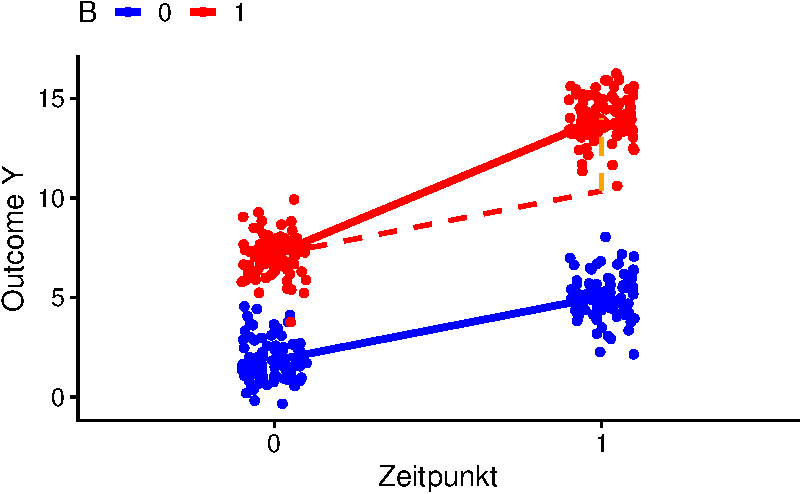
\includegraphics{DiD_files/figure-pdf/fig-DIDSIMB-1.pdf}

}

\caption{\label{fig-DIDSIMB}Einfache DID-Schätzung mit R für simulierte
Daten}

\end{figure}%

\section{Case Study: Effekt von Steuererleichterungen auf
Erwerbsbeteilligung}\label{case-study-effekt-von-steuererleichterungen-auf-erwerbsbeteilligung}

Der
\href{https://www.irs.gov/credits-deductions/individuals/earned-income-tax-credit-eitc}{Earned
Income Tax Credit} (EITC) ist ein Steuerguthaben für US-Amerkanische
Familien, die unterhalb einer gesetztlich festgelegten Einkoemmnsgrenze
liegen. Der genaue Betrag des EITC hängt gestaffelt vom Einkommen ab
und, ähnlich zum Kindergeld in Deutschland, steigt mit der Anzahl der zu
versorgenden Kinder. Ein wichtiger Unterschied zum Kindergeld ist, dass
der EITC nicht beantragt werden muss: Qualifizierten Familien wird der
Betrag automatisch durch die Behörden im Jahressteuerausgleich
gutgeschrieben. Somit kann Selbstselektion in die Behandlungsgruppe
ausgeschlossen werden, da sich die Behandlung ausschließlich durch die
im Rahmen der EITC-Ausweitung geänderten Anspruchsgrundlagen ergibt.

Eissa und Liebman (1996) betrachten Veränderungen in der
EITC-Gesetzgebung als Intervention, deren Auswirkungen mit
sozio-ökonomischen Paneldaten in einem DID-Ansatz untersucht werden
können. Die Studie analysiert die Auswirkungen der ersten Ausweitung des
EITC im Jahr 1986 auf die Erwerbsbeteiligung und die Löhne von Müttern
im erwerbsfähigen Alter. Diese Erweiterung erhöhte die gewährten
Steuererleichterungen und die zur Qualifikation für das Programm zu
unterschreitende Einkommensgrenze.

Ein zentraler Befund der Studie ist, dass die EITC-Ausweitung von 1986
einen statistisch signifikanten Anstieg der Arbeitsbeteiligung
alleinerziehender Frauen von geschätzten 3\% bewirkt hat. Eissa und
Liebman (1996) finden weiterhin signifikante positive Effekte auf die
geleisteten Arbeitsstunden und Evidenz für Einkommensverbesserungen in
dieser Gruppe. Die Studienergebnisse sind starke Evidenz, dass Maßnahmen
wie der EITC effektiv dazu beitragen können, die Erwerbssituation in der
Zielgruppe zu steigern und somit die wirtsschafts- und sozialpolitische
Ziele derartiger Programme realisierbar sind.

Im Jahr 1993 wurde das Programm erneut ausgweitet: Vor 1993 gab es
lediglich eine Einkommensstufe für Familien mit Kindern. 1993 wurde eine
zusätzliche Stufe für Familien mit zwei oder mehr Kindern eigeführt, die
damit einen höheren maximalen Kreditbetrag erhalten konnten als Familien
mit nur einem Kind. Dies führte zu einer größeren steuerlichen
Entlastung armutsbedrohter Familien.

Adireksombat (2010) untersucht die Effekte der zweiten EITC-Ausweitung
ebenfalls mit einem DID Ansatz und findet Evidenz für einen Anstieg der
Arbeitbeteiligung von etwa 5\% in der Zielgruppe alleinerziehender
Frauen mit mindestens 2 Kindern.

Zur Illustration der empirischen Anwendung von DID mit R untersuchen wir
Effekte der EITC-Ausweitung von 1993 nachfolgend anhand eines ähnlichen
Datensatzes aus dem
\href{https://www.census.gov/programs-surveys/cps.html}{CPS} wie in der
Studie von Adireksombat (2010). Diese Daten umfassen jährliche
sozio-ökonomische Merkmale für US-amerikanische Frauen im Zeitraum von
1991 bis 1996 und sind in der Datei \texttt{eitc\_data.csv} verfügbar.

Wir lesen den Datensatz zunächst ein.

\begin{Shaded}
\begin{Highlighting}[]
\FunctionTok{library}\NormalTok{(readr)}

\CommentTok{\# EITC{-}Datensatz einlesen}
\NormalTok{eitc\_data }\OtherTok{\textless{}{-}} \FunctionTok{read\_csv}\NormalTok{(}\StringTok{"datasets/eitc\_data.csv"}\NormalTok{)}
\end{Highlighting}
\end{Shaded}

Eine Übersicht des Datensatzes \texttt{eitc\_data} ist in
Tabelle~\ref{tbl-EITCdata} dargestellt.

\begin{longtable}{ll}

\caption{\label{tbl-EITCdata}Sozi-ökomonische Variablen zu US-Familien
aus dem CPS}

\tabularnewline

\toprule
Variable & Beschreibung \\ 
\midrule\addlinespace[2.5pt]
state & ID-Code Bundesstaat \\ 
year & Steuerjahr \\ 
urate & Arbeitslosenquote im Bundesstaat (\%) \\ 
children & Anz. Kinder der Frau \\ 
nonwhite & Dummy für nicht-weiße Frauen \\ 
finc & Haushaltseinkommen im Steuerjahr (US-\$) \\ 
earn & Einkommen der Frau im Steuerjahr (US-\$) \\ 
age & Alter \\ 
ed & Ausbildungsniveau der Frau (Jahre) \\ 
work & Dummy für Berufstätigkeit \\ 
unearn & = Haushaltseinkommen - Einkommen der Frau (Tsd. US-\$)  \\ 
\bottomrule

\end{longtable}

Wir erweitern das \texttt{tibble}-Objekt zunächst um eine Dummy-Variable
für Mütter (\texttt{anykids}), sowie spezifischere Dummies für Frauen
mit einem Kind (\texttt{onechild}) oder mit zwei oder mehr Kindern
(\texttt{twomorekids}). Weiterhin erzeugen wir einen Indikator für
Beobachtungen \emph{nach} der EITC-Ausweitung im Jahr 1993
(\texttt{after1993}).

\begin{Shaded}
\begin{Highlighting}[]
\CommentTok{\# Dummies für Frauen mit Kindern}
\CommentTok{\# und Post{-}Interventionsprediode hinzufügen }
\NormalTok{eitc\_data }\OtherTok{\textless{}{-}}\NormalTok{ eitc\_data }\SpecialCharTok{\%\textgreater{}\%}
  \FunctionTok{mutate}\NormalTok{(}
    \AttributeTok{onechild =} \FunctionTok{if\_else}\NormalTok{(children }\SpecialCharTok{==} \DecValTok{1}\NormalTok{, }\ConstantTok{TRUE}\NormalTok{, }\ConstantTok{FALSE}\NormalTok{),}
    \AttributeTok{twomorekids =} \FunctionTok{if\_else}\NormalTok{(children }\SpecialCharTok{\textgreater{}=} \DecValTok{2}\NormalTok{, }\ConstantTok{TRUE}\NormalTok{, }\ConstantTok{FALSE}\NormalTok{),}
    \AttributeTok{anykids =} \FunctionTok{if\_else}\NormalTok{(children }\SpecialCharTok{\textgreater{}} \DecValTok{0}\NormalTok{, }\ConstantTok{TRUE}\NormalTok{, }\ConstantTok{FALSE}\NormalTok{),}
    \AttributeTok{after1993 =} \FunctionTok{if\_else}\NormalTok{(year }\SpecialCharTok{\textgreater{}} \DecValTok{1993}\NormalTok{, }\ConstantTok{TRUE}\NormalTok{, }\ConstantTok{FALSE}\NormalTok{)}
\NormalTok{  )}
\end{Highlighting}
\end{Shaded}

Einen Überblick über den modifizierten Datensatz erhalten wir mit
\texttt{glimpse()}.

\begin{Shaded}
\begin{Highlighting}[]
\CommentTok{\# Modifikationen kontrollieren}
\FunctionTok{glimpse}\NormalTok{(eitc\_data)}
\end{Highlighting}
\end{Shaded}

\begin{verbatim}
Rows: 13,746
Columns: 15
$ state       <dbl> 11, 12, 13, 14, 15, 16, 21, 22, 23, 31, 32, 33, 34, 35, 41~
$ year        <dbl> 1991, 1991, 1991, 1991, 1991, 1991, 1991, 1991, 1991, 1991~
$ urate       <dbl> 7.6, 7.2, 6.4, 9.1, 8.6, 6.8, 7.3, 6.7, 7.0, 6.4, 6.0, 7.2~
$ children    <dbl> 0, 1, 2, 0, 3, 1, 0, 0, 1, 2, 0, 2, 0, 0, 0, 1, 1, 0, 0, 0~
$ nonwhite    <dbl> 1, 0, 0, 1, 1, 0, 1, 1, 1, 1, 0, 0, 0, 0, 1, 0, 0, 0, 0, 0~
$ finc        <dbl> 18714, 4839, 8178, 9370, 14707, 21605, 19147, 64312, 17676~
$ earn        <dbl> 18714.4, 471.4, 0.0, 0.0, 14706.6, 18854.6, 14141.0, 63802~
$ age         <dbl> 26, 22, 33, 43, 23, 53, 52, 51, 20, 32, 51, 29, 54, 28, 27~
$ ed          <dbl> 10, 9, 11, 11, 7, 7, 11, 11, 11, 11, 9, 10, 9, 11, 11, 7, ~
$ work        <dbl> 1, 1, 0, 0, 1, 1, 1, 1, 1, 1, 1, 1, 0, 0, 0, 0, 0, 1, 1, 1~
$ unearn      <dbl> 0.0000, 4.3672, 8.1782, 9.3696, 0.0000, 2.7504, 5.0059, 0.~
$ onechild    <lgl> FALSE, TRUE, FALSE, FALSE, FALSE, TRUE, FALSE, FALSE, TRUE~
$ twomorekids <lgl> FALSE, FALSE, TRUE, FALSE, TRUE, FALSE, FALSE, FALSE, FALS~
$ anykids     <lgl> FALSE, TRUE, TRUE, FALSE, TRUE, TRUE, FALSE, FALSE, TRUE, ~
$ after1993   <lgl> FALSE, FALSE, FALSE, FALSE, FALSE, FALSE, FALSE, FALSE, FA~
\end{verbatim}

Die Plausibilität der Annahme paralleler Trends können wir graphisch
anhand einer Gegenüberstellung der \emph{Beschäftigungsquote}
(\texttt{avg.work\ =\ mean(work)}) für Frauen mit und ohne Kindern
(\texttt{anykids}) über die Zeit (\texttt{year}) einschätzen. Wir
gruppieren hierzu den Datensatz entsprechend und fassen die
Outcome-Variable (\texttt{work}) gruppenweise zusammen.

\begin{Shaded}
\begin{Highlighting}[]
\CommentTok{\# Zeitpunkt{-}Gruppen{-}Mittelwerte berechnen}
\NormalTok{(}
\NormalTok{  eitc\_summarised }\OtherTok{\textless{}{-}}\NormalTok{ eitc\_data }\SpecialCharTok{\%\textgreater{}\%}
  \FunctionTok{group\_by}\NormalTok{(year, anykids) }\SpecialCharTok{\%\textgreater{}\%}
  \FunctionTok{summarise}\NormalTok{(}
    \AttributeTok{avg.work =} \FunctionTok{mean}\NormalTok{(work)}
\NormalTok{  )}
\NormalTok{)}
\end{Highlighting}
\end{Shaded}

\begin{verbatim}
# A tibble: 12 x 3
# Groups:   year [6]
    year anykids avg.work
   <dbl> <lgl>      <dbl>
 1  1991 FALSE       0.58
 2  1991 TRUE        0.46
 3  1992 FALSE       0.57
 4  1992 TRUE        0.44
 5  1993 FALSE       0.57
 6  1993 TRUE        0.44
 7  1994 FALSE       0.59
 8  1994 TRUE        0.46
 9  1995 FALSE       0.57
10  1995 TRUE        0.51
11  1996 FALSE       0.55
12  1996 TRUE        0.50
\end{verbatim}

\begin{Shaded}
\begin{Highlighting}[]
\CommentTok{\# Graphischer Vergleich der Trends}
\FunctionTok{ggplot}\NormalTok{(}\AttributeTok{data =}\NormalTok{ eitc\_summarised) }\SpecialCharTok{+}
  \FunctionTok{geom\_line}\NormalTok{(}
    \AttributeTok{mapping =} \FunctionTok{aes}\NormalTok{(}
      \AttributeTok{x =}\NormalTok{ year, }
      \AttributeTok{y =}\NormalTok{ avg.work, }
      \AttributeTok{col =}\NormalTok{ anykids}
\NormalTok{    )}
\NormalTok{  ) }\SpecialCharTok{+}
  \CommentTok{\# Indikator für EITC{-}Erweiterung 1993}
  \FunctionTok{geom\_vline}\NormalTok{(}
    \AttributeTok{xintercept =} \DecValTok{1993}\NormalTok{, }
    \AttributeTok{lty =} \StringTok{"dashed"}
\NormalTok{  ) }\SpecialCharTok{+}
  \FunctionTok{scale\_x\_continuous}\NormalTok{(}\StringTok{"Jahr"}\NormalTok{) }\SpecialCharTok{+}
  \FunctionTok{scale\_y\_continuous}\NormalTok{(}\StringTok{"Beschäftigungsquote"}\NormalTok{) }\SpecialCharTok{+}
  \FunctionTok{scale\_color\_manual}\NormalTok{(}
    \AttributeTok{values =} \FunctionTok{c}\NormalTok{(}\StringTok{"TRUE"} \OtherTok{=} \StringTok{"red"}\NormalTok{, }\StringTok{"FALSE"} \OtherTok{=} \StringTok{"blue"}\NormalTok{)}
\NormalTok{  ) }\SpecialCharTok{+}
  \FunctionTok{guides}\NormalTok{(}\AttributeTok{color =} \FunctionTok{guide\_legend}\NormalTok{(}\AttributeTok{title =} \StringTok{"Kinder?"}\NormalTok{)) }\SpecialCharTok{+}
  \FunctionTok{theme\_cowplot}\NormalTok{()}
\end{Highlighting}
\end{Shaded}

\begin{figure}[t]

\centering{

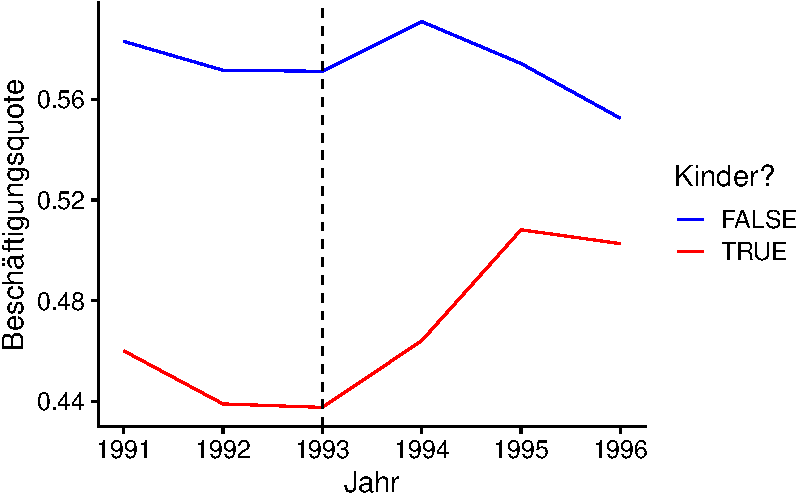
\includegraphics{DiD_files/figure-pdf/fig-EITCtrends-1.pdf}

}

\caption{\label{fig-EITCtrends}Trends in der Erwerbsbeteiligung
US-amerikanischer Frauen im CPS-Datensatz}

\end{figure}%

Abbildung~\ref{fig-EITCtrends} zeigt, dass die Beschäftigungsquote für
kinderlose Frauen deutlich oberhalb der Quote für Mütter verläuft. Die
Trends vor der EITC-Ausweitung im Jahr 1993 sind sehr ähnlich, sodass
eine parallele Entwicklung plausibel scheint.

\subsection{Schätzungen des ATT mit linearen
Modellen}\label{sec-didattest}

Wir berechnen Zunächst den Behandlungseffekt der für Frauen mit Kindern
relativ zu kinderlosen Frauen gemäß \eqref{eq:DIDMOMENTS}, wobei wir
jeweils \emph{sämtliche} Perioden vor und nach der Behandlung
einbeziehen. Dies führt zu den Ergebnissen in Tabelle~\ref{tbl-EITCSM},
wobei \begin{align}
  \textcolor{orange}{\widehat\beta_\text{DID}} = (\textcolor{red}{B} - \textcolor{red}{A}) - (\textcolor{blue}{D} - \textcolor{blue}{C})
\end{align} der geschätzte Behandlungseffekt ist.

\begin{longtable}[]{@{}
  >{\raggedright\arraybackslash}p{(\columnwidth - 6\tabcolsep) * \real{0.3390}}
  >{\centering\arraybackslash}p{(\columnwidth - 6\tabcolsep) * \real{0.2119}}
  >{\centering\arraybackslash}p{(\columnwidth - 6\tabcolsep) * \real{0.2119}}
  >{\centering\arraybackslash}p{(\columnwidth - 6\tabcolsep) * \real{0.2373}}@{}}
\caption{\texttt{eitc\_data}: Stichprobenmittelwerte für
\texttt{work}}\label{tbl-EITCSM}\tabularnewline
\toprule\noalign{}
\begin{minipage}[b]{\linewidth}\raggedright
\end{minipage} & \begin{minipage}[b]{\linewidth}\centering
v. EITC-Ausweitung
\end{minipage} & \begin{minipage}[b]{\linewidth}\centering
n.~EITC-Ausweitung
\end{minipage} & \begin{minipage}[b]{\linewidth}\centering
Differenz
\end{minipage} \\
\midrule\noalign{}
\endfirsthead
\toprule\noalign{}
\begin{minipage}[b]{\linewidth}\raggedright
\end{minipage} & \begin{minipage}[b]{\linewidth}\centering
v. EITC-Ausweitung
\end{minipage} & \begin{minipage}[b]{\linewidth}\centering
n.~EITC-Ausweitung
\end{minipage} & \begin{minipage}[b]{\linewidth}\centering
Differenz
\end{minipage} \\
\midrule\noalign{}
\endhead
\bottomrule\noalign{}
\endlastfoot
\textbf{Kinder} & \(\textcolor{red}{A = .446}\) &
\(\textcolor{red}{B = .491}\) & \(\textcolor{red}{.045}\) \\
\textbf{k. Kinder} & \(\textcolor{blue}{C = .575}\) &
\(\textcolor{blue}{D = .573}\) & \(\textcolor{blue}{-.002}\) \\
\(\textcolor{orange}{\widehat{\beta}_\text{DID}}\) & & &
\(\textcolor{orange}{.047}\) \\
\end{longtable}

Die nachfolgenden Code-Chunks zeigen die Schritte zur Berechnung von
\(\widehat{\beta}_\text{DID}\) mit R.

\begin{Shaded}
\begin{Highlighting}[]
\CommentTok{\# A, B, C und D berechnen}
\NormalTok{(}
\NormalTok{  ABCD }\OtherTok{\textless{}{-}}\NormalTok{ eitc\_data }\SpecialCharTok{\%\textgreater{}\%}
    \FunctionTok{group\_by}\NormalTok{(after1993, anykids) }\SpecialCharTok{\%\textgreater{}\%}
    \FunctionTok{summarise}\NormalTok{(}\AttributeTok{avg.work =} \FunctionTok{mean}\NormalTok{(work))}
\NormalTok{)}
\end{Highlighting}
\end{Shaded}

\begin{verbatim}
# A tibble: 4 x 3
# Groups:   after1993 [2]
  after1993 anykids avg.work
  <lgl>     <lgl>      <dbl>
1 FALSE     FALSE       0.58
2 FALSE     TRUE        0.45
3 TRUE      FALSE       0.57
4 TRUE      TRUE        0.49
\end{verbatim}

\begin{Shaded}
\begin{Highlighting}[]
\CommentTok{\# Differenzen bilden}
\NormalTok{DminusC }\OtherTok{\textless{}{-}}\NormalTok{ ABCD }\SpecialCharTok{\%\textgreater{}\%}
    \FunctionTok{filter}\NormalTok{(anykids }\SpecialCharTok{==} \ConstantTok{FALSE}\NormalTok{) }\SpecialCharTok{\%\textgreater{}\%}
    \FunctionTok{pull}\NormalTok{(avg.work) }\SpecialCharTok{\%\textgreater{}\%}
    \FunctionTok{diff}\NormalTok{()}

\NormalTok{BminusA }\OtherTok{\textless{}{-}}\NormalTok{ ABCD }\SpecialCharTok{\%\textgreater{}\%}
    \FunctionTok{filter}\NormalTok{(anykids }\SpecialCharTok{==} \ConstantTok{TRUE}\NormalTok{) }\SpecialCharTok{\%\textgreater{}\%}
    \FunctionTok{pull}\NormalTok{(avg.work) }\SpecialCharTok{\%\textgreater{}\%}
    \FunctionTok{diff}\NormalTok{()}
\end{Highlighting}
\end{Shaded}

\begin{Shaded}
\begin{Highlighting}[]
\CommentTok{\# DID{-}Schätzung: Differenz der Stichprobenmittel{-}Differenzen}
\NormalTok{beta\_DID\_means }\OtherTok{\textless{}{-}}\NormalTok{ BminusA }\SpecialCharTok{{-}}\NormalTok{ DminusC}
\NormalTok{beta\_DID\_means}
\end{Highlighting}
\end{Shaded}

\begin{verbatim}
[1] 0.04687
\end{verbatim}

Durch Iteration von \texttt{summarise()} können wir diese Rechenschritte
effizienter ausführen.

\begin{Shaded}
\begin{Highlighting}[]
\CommentTok{\# Effizienter:}
\NormalTok{eitc\_data  }\SpecialCharTok{\%\textgreater{}\%} 
    \FunctionTok{group\_by}\NormalTok{(after1993, anykids) }\SpecialCharTok{\%\textgreater{}\%} 
    \FunctionTok{summarise}\NormalTok{(}\AttributeTok{avg.work =} \FunctionTok{mean}\NormalTok{(work)) }\SpecialCharTok{\%\textgreater{}\%}
    \FunctionTok{summarise}\NormalTok{(}\AttributeTok{diff\_time =} \FunctionTok{diff}\NormalTok{(avg.work)) }\SpecialCharTok{\%\textgreater{}\%}
    \FunctionTok{summarise}\NormalTok{(}\AttributeTok{beta\_DID\_means =} \FunctionTok{diff}\NormalTok{(diff\_time)) }\SpecialCharTok{\%\textgreater{}\%}
    \FunctionTok{pull}\NormalTok{(beta\_DID\_means)}
\end{Highlighting}
\end{Shaded}

\begin{verbatim}
[1] 0.04687
\end{verbatim}

Wir erhalten also eine positive Schätzung des Behandlungseffekts. Die
Interpretation ist, dass die Ausweitung des EITC im Jahr 1993 zu einem
Anstieg der Erwerbsbeteiligung in der Gruppe der Frauen mit Kindern von
durchschittlich \(4.69\%\) in den Folgeperioden geführt hat.

Für die Berechnung von Inferenzstatistiken bezüglich
\(\beta_\text{DID}\) schätzen wir ein lineares Interaktionsmodell gemäß
\eqref{eq:DIDREG},

\begin{align}
  \begin{split}
    \text{work}_{i,t} =&\, \beta_0 + \beta_1 \text{anykids}_{i,t} + \beta_2 \text{after1993}_t \\
  +&\, \beta_3 (\text{anykids}_{i,t} \times \text{after1993}_t) + \epsilon_{i,t}.
  \end{split}\label{eq:eitcmod}
\end{align}

\begin{Shaded}
\begin{Highlighting}[]
\CommentTok{\# Equivalente Schätzung u. Inferenz }
\CommentTok{\# mit linearem Interaktionsmodell}
\NormalTok{DiD\_reg }\OtherTok{\textless{}{-}} \FunctionTok{lm}\NormalTok{(}
  \AttributeTok{formula =}\NormalTok{ work }\SpecialCharTok{\textasciitilde{}}\NormalTok{ anykids }\SpecialCharTok{*}\NormalTok{ after1993, }
  \AttributeTok{data =}\NormalTok{ eitc\_data}
\NormalTok{)}
\end{Highlighting}
\end{Shaded}

Der geschätzte Koeffizient des Interkationsterms stimmt mit der händisch
berechneten Schätzung überein.

\begin{Shaded}
\begin{Highlighting}[]
\FunctionTok{tidy}\NormalTok{(DiD\_reg) }\SpecialCharTok{\%\textgreater{}\%} 
  \FunctionTok{filter}\NormalTok{(term }\SpecialCharTok{==} \StringTok{"anykidsTRUE:after1993TRUE"}\NormalTok{) }\SpecialCharTok{\%\textgreater{}\%} 
  \FunctionTok{pull}\NormalTok{(estimate)}
\end{Highlighting}
\end{Shaded}

\begin{verbatim}
[1] 0.04687
\end{verbatim}

Mit \texttt{coeftest()} berechnen wir heteroskedastie-robuste
Inferenzstatistiken.

\begin{Shaded}
\begin{Highlighting}[]
\CommentTok{\# Robuste Inferenzstatistiken}
\FunctionTok{coeftest}\NormalTok{(}
  \AttributeTok{x =}\NormalTok{ DiD\_reg, }
  \AttributeTok{vcov. =}\NormalTok{ vcovHC, }
  \AttributeTok{type =} \StringTok{"HC1"}
\NormalTok{)}
\end{Highlighting}
\end{Shaded}

\begin{verbatim}

t test of coefficients:

                          Estimate Std. Error t value Pr(>|t|)    
(Intercept)                0.57546    0.00880   65.38   <2e-16 ***
anykidsTRUE               -0.12950    0.01165  -11.12   <2e-16 ***
after1993TRUE             -0.00207    0.01287   -0.16   0.8720    
anykidsTRUE:after1993TRUE  0.04687    0.01714    2.73   0.0063 ** 
---
Signif. codes:  0 '***' 0.001 '**' 0.01 '*' 0.05 '.' 0.1 ' ' 1
\end{verbatim}

Der Koeffizient des Interaktionsterms ist zum 1\%-Niveau signifikant.
\texttt{fixest::feols()} liefert eine identische Schätzung.

\begin{Shaded}
\begin{Highlighting}[]
\FunctionTok{library}\NormalTok{(fixest)}
\NormalTok{(}
\NormalTok{  DID\_twoway }\OtherTok{\textless{}{-}} \FunctionTok{feols}\NormalTok{(}
    \AttributeTok{fml =}\NormalTok{ work }\SpecialCharTok{\textasciitilde{}}\NormalTok{ anykids }\SpecialCharTok{*}\NormalTok{ after1993,}
    \AttributeTok{data =}\NormalTok{ eitc\_data, }
    \AttributeTok{vcov =} \StringTok{"HC1"}
\NormalTok{  )}
\NormalTok{)}
\end{Highlighting}
\end{Shaded}

\begin{verbatim}
OLS estimation, Dep. Var.: work
Observations: 13,746
Standard-errors: Heteroskedasticity-robust 
                           Estimate Std. Error  t value  Pr(>|t|)    
(Intercept)                0.575460   0.008802  65.3756 < 2.2e-16 ***
anykidsTRUE               -0.129498   0.011648 -11.1176 < 2.2e-16 ***
after1993TRUE             -0.002074   0.012873  -0.1611 0.8720396    
anykidsTRUE:after1993TRUE  0.046873   0.017144   2.7342 0.0062619 ** 
---
Signif. codes:  0 '***' 0.001 '**' 0.01 '*' 0.05 '.' 0.1 ' ' 1
RMSE: 0.496672   Adj. R2: 0.012384
\end{verbatim}

Wir erweitern Modell \eqref{eq:eitcmod} nun um Fixed Effekts für den
\href{https://cps.ipums.org/cps-action/variables/statefip}{US-Bundesstaat}
sowie das Jahr,

\begin{align}
  \begin{split}
    \text{work}_{i,t} =&\, \theta_\text{Staat} + \eta_t \\
    +&\, \beta_1 \text{anykids}_{i,t} + \beta_2 (\text{anykids}_{i,t} \times \text{after1993}_t) + \epsilon_{i,t}.
    \end{split}\label{eq:eitcmodfe}
\end{align}

Anhand der Dummy-Variablen für Bundesstaaten (\(\theta_\text{Staat}\))
und Jahre (\(\eta_t\)) kontrollieren wir für unbeobachtete
zeitinvariante Unterschiede zwischen den Bundesstaaten sowie für
allgemeine zeitliche Trends und Schocks, die alle Bundesstaaten in einem
bestimmten Jahr betreffen. Dies schließt etwaige Backdoor-Pfade durch
den Einfluss spezifischer Eigenschaften der Bundesstaaten (Kultur,
Geografie, langfristige politische Einstellungen, etc.) und gemeinsamer
zeitlicher Einflüsse.

\begin{Shaded}
\begin{Highlighting}[]
\FunctionTok{library}\NormalTok{(fixest)}
\NormalTok{(}
\NormalTok{  DID\_twoway }\OtherTok{\textless{}{-}} \FunctionTok{feols}\NormalTok{(}
    \AttributeTok{fml =}\NormalTok{ work }\SpecialCharTok{\textasciitilde{}}\NormalTok{ anykids }\SpecialCharTok{+} \FunctionTok{I}\NormalTok{(anykids }\SpecialCharTok{*}\NormalTok{ after1993) }
    \SpecialCharTok{|}\NormalTok{ state }\SpecialCharTok{+}\NormalTok{ year,}
    \AttributeTok{data =}\NormalTok{ eitc\_data}
\NormalTok{  )}
\NormalTok{)}
\end{Highlighting}
\end{Shaded}

\begin{verbatim}
OLS estimation, Dep. Var.: work
Observations: 13,746
Fixed-effects: state: 51,  year: 6
Standard-errors: Clustered (state) 
                       Estimate Std. Error t value   Pr(>|t|)    
anykidsTRUE            -0.12391    0.01593  -7.776 3.6952e-10 ***
I(anykids * after1993)  0.04579    0.01656   2.765 7.9497e-03 ** 
---
Signif. codes:  0 '***' 0.001 '**' 0.01 '*' 0.05 '.' 0.1 ' ' 1
RMSE: 0.489063     Adj. R2: 0.038633
                 Within R2: 0.011101
\end{verbatim}

Die Schätzung des ATT bei Kontrolle für Zeit- und Bundesstaat-Effekte in
\eqref{eq:eitcmodfe} unterscheidet sich nur geringfügig gegenüber dem
Ergebnis für das Modell \eqref{eq:eitcmod}. Beachte, dass der
Behandlungseffekt auch bei geclusterten Standardfehlern auf
Bundesstaaten-Ebene (\texttt{\textbar{}\ state\ +\ year}) signifikant
ist.

Ein weiterer Vorteil von DID-Schätzungen mit Regression ist die
Möglichkeit zur Kontrolle für individuen-spezifische Kovariablen, um
Backdoors aufgrund systematischer Unterschiede zwischen Kontroll- und
Behandlungsgruppen zu vermeiden.

Wir erweitern Modell \eqref{eq:eitcmodfec} um sozio-ökonomische
Charakteristika der Frauen: Einen Dummy für nicht-weiße Frauen
(\texttt{nonwhite}), quadratische Terme in Alter (\texttt{age}) und
Ausbildungsniveau (\texttt{ed}) sowie weitere Einkünfte des Haushalts
(\texttt{unearn}),

\begin{align}
  \begin{split}
    \text{work}_{i,t} =&\, \theta_\text{Staat} + \eta_t \\
    +&\, \beta_1 \text{anykids}_{i,t} + \beta_2 (\text{anykids}_{i,t} \times \text{after1993}_t) \\
    +&\, \beta_3 \text{unearn} + \beta_4 \text{nonwhite} \\
    +&\, \beta_5 \text{age} + \beta_6 \text{age}^2 + \beta_7 \text{ed} + \beta_8 \text{ed}^2 \\
    +&\, \epsilon_{i,t}.
    \end{split}\label{eq:eitcmodfec}
\end{align}

\begin{Shaded}
\begin{Highlighting}[]
\CommentTok{\# Year{-}FE + State{-}FE + Kontrollvariablen}
\NormalTok{(}
\NormalTok{  DID\_FE\_controls }\OtherTok{\textless{}{-}} \FunctionTok{feols}\NormalTok{(}
    \AttributeTok{fml =}\NormalTok{ work }\SpecialCharTok{\textasciitilde{}}\NormalTok{ anykids }\SpecialCharTok{+} \FunctionTok{I}\NormalTok{(anykids }\SpecialCharTok{*}\NormalTok{ after1993) }
    
    \SpecialCharTok{+}\NormalTok{ unearn }\SpecialCharTok{+}\NormalTok{ nonwhite }
    \SpecialCharTok{+}\NormalTok{ age }\SpecialCharTok{+} \FunctionTok{I}\NormalTok{(age}\SpecialCharTok{\^{}}\DecValTok{2}\NormalTok{)}
    \SpecialCharTok{+}\NormalTok{ ed }\SpecialCharTok{+} \FunctionTok{I}\NormalTok{(ed}\SpecialCharTok{\^{}}\DecValTok{2}\NormalTok{)}
    
    \SpecialCharTok{|}\NormalTok{ state }\SpecialCharTok{+}\NormalTok{ year, }
    
    \AttributeTok{data =}\NormalTok{ eitc\_data}
\NormalTok{  )}
\NormalTok{)}
\end{Highlighting}
\end{Shaded}

\begin{verbatim}
OLS estimation, Dep. Var.: work
Observations: 13,746
Fixed-effects: state: 51,  year: 6
Standard-errors: Clustered (state) 
                        Estimate Std. Error  t value   Pr(>|t|)    
anykidsTRUE            -0.119221   0.010673 -11.1709 3.4010e-15 ***
I(anykids * after1993)  0.055755   0.014385   3.8759 3.1021e-04 ***
unearn                 -0.017695   0.000959 -18.4575  < 2.2e-16 ***
nonwhite               -0.080399   0.028048  -2.8665 6.0589e-03 ** 
age                     0.026323   0.003664   7.1847 3.0857e-09 ***
I(age^2)               -0.000316   0.000052  -6.0298 1.9673e-07 ***
ed                     -0.004160   0.006270  -0.6634 5.1013e-01    
I(ed^2)                 0.001536   0.000535   2.8701 6.0002e-03 ** 
---
Signif. codes:  0 '***' 0.001 '**' 0.01 '*' 0.05 '.' 0.1 ' ' 1
RMSE: 0.46896     Adj. R2: 0.115657
                Within R2: 0.090729
\end{verbatim}

Die Schätzung von \eqref{eq:eitcmodfec} ergibt mit \(0.0558\) eine etwas
größere Schätzung eines positiven signifikanten Effekt der
EITC-Ausweitung auf die Erwerbsbeteiligung von Müttern.

Wie oben erläutert, führte die EITC-Ausweitung von 1993 unter anderem
ein Stufensystem für die Höhe des EITC in Ahängigkeit der Kinder-Anzahl
ein, sodass unterschiedlich starke Anreize zur Aufnahme einer
Beschäftigung für Mütter mit nur einem Kind und mehreren Kindern
plausibel sind. Anhand der Dummy-Variablen für (genau) ein Kind
(\texttt{onechild}) sowie zwei oder mehr Kinder (\texttt{twomorekids})
können wir eine differenziertere Schätzung des Effekts hinsichtlich des
Betreuungsaufwands erhalten. Hierzu modifizieren wir Modell
\eqref{eq:eitcmodfec} entsprechend:

\begin{align}
  \begin{split}
    \text{work}_{i,t} =&\, \theta_\text{Staat} + \eta_t \\
    +&\, \beta_1 \text{onechild}_{i,t} + \beta_2 (\text{onechild}_{i,t} \times \text{after1993}_t) \\
    +&\, \beta_3 \text{twomorechild}_{i,t} + \beta_4 (\text{twomorechild}_{i,t} \times \text{after1993}_t) \\
    +&\, \beta_5 \text{unearn} + \beta_6 \text{nonwhite} + \beta_7 \text{age} + \beta_8 \text{age}^2 + \beta_9 \text{ed} + \beta_{10} \text{ed}^2 \\
    +&\, \epsilon_{i,t}.
  \end{split}\label{eq:eitcmodfecd}
\end{align}

\begin{Shaded}
\begin{Highlighting}[]
\CommentTok{\# Differenzierung: onechild / twomorekids}
\NormalTok{(}
\NormalTok{  DID\_FE\_spec\_controls }\OtherTok{\textless{}{-}} \FunctionTok{feols}\NormalTok{(}
    \AttributeTok{fml =}\NormalTok{ work }\SpecialCharTok{\textasciitilde{}} 
\NormalTok{      onechild }\SpecialCharTok{+} \FunctionTok{I}\NormalTok{(onechild }\SpecialCharTok{*}\NormalTok{ after1993) }
    \SpecialCharTok{+}\NormalTok{ twomorekids }\SpecialCharTok{+} \FunctionTok{I}\NormalTok{(twomorekids }\SpecialCharTok{*}\NormalTok{ after1993) }
    
    \SpecialCharTok{+}\NormalTok{ unearn }\SpecialCharTok{+}\NormalTok{ nonwhite }
    \SpecialCharTok{+}\NormalTok{ age }\SpecialCharTok{+} \FunctionTok{I}\NormalTok{(age}\SpecialCharTok{\^{}}\DecValTok{2}\NormalTok{)}
    \SpecialCharTok{+}\NormalTok{ ed }\SpecialCharTok{+} \FunctionTok{I}\NormalTok{(ed}\SpecialCharTok{\^{}}\DecValTok{2}\NormalTok{)}
    
    \SpecialCharTok{|}\NormalTok{ state }\SpecialCharTok{+}\NormalTok{ year,}
    
    \AttributeTok{data =}\NormalTok{ eitc\_data}
\NormalTok{  )}
\NormalTok{)}
\end{Highlighting}
\end{Shaded}

\begin{verbatim}
OLS estimation, Dep. Var.: work
Observations: 13,746
Fixed-effects: state: 51,  year: 6
Standard-errors: Clustered (state) 
                            Estimate Std. Error  t value   Pr(>|t|)    
onechildTRUE               -0.063581   0.013327  -4.7708 1.6319e-05 ***
I(onechild * after1993)     0.040539   0.017829   2.2737 2.7311e-02 *  
twomorekidsTRUE            -0.161675   0.013127 -12.3166  < 2.2e-16 ***
I(twomorekids * after1993)  0.064799   0.016411   3.9485 2.4649e-04 ***
unearn                     -0.017334   0.000992 -17.4790  < 2.2e-16 ***
nonwhite                   -0.073759   0.027833  -2.6501 1.0745e-02 *  
age                         0.028990   0.003475   8.3433 4.9204e-11 ***
I(age^2)                   -0.000357   0.000049  -7.2889 2.1209e-09 ***
ed                         -0.003765   0.006350  -0.5929 5.5595e-01    
I(ed^2)                     0.001517   0.000552   2.7474 8.3318e-03 ** 
---
Signif. codes:  0 '***' 0.001 '**' 0.01 '*' 0.05 '.' 0.1 ' ' 1
RMSE: 0.467886     Adj. R2: 0.119572
                 Within R2: 0.094887
\end{verbatim}

Die interessierenden geschätzten Koeffizienten von
\texttt{I(onechild\ *\ after1993)} und
\texttt{I(twomorekids\ *\ after1993)} sind \(0.0405\) und \(0.0648\).
Auch hier sind die Koeffizienten signifikant von null verschieden. Der
größere Koeffizient für den Effekt auf Mütter mit zwei oder mehr Kinder
liefert Evidenz dafür, dass die Einführung der Zahlstufe für größere
Familien im Rahmen der EITC-Ausweitung von 1993 tatsächlich einen etwas
stärkeren Anreiz auf die Zielgruppe mit mehreren Kindern hatte.

\subsection{Probit-Spezifikationen}\label{sec-eitc-probit}

In sämtlichen Modellen in Kapitel~\ref{sec-didattest} haben wir
\(\text{work}_{i,t}\) als kontinulierliche Variable behandelt und den
bedingten Erwartungswert als lineare Funktion modelliert. Da
\(\text{work}_{i,t}\) eine binäre Variable ist, haben wir damit implizit
die bedingte \emph{Wahrscheinlichkeit} der Erwerbsbeteiligung
\(P(\text{work}_{i,t} = 1\vert \boldsymbol{x}_{i,t})\) modelliert. Wie
in Kapitel~\ref{sec-lpm} erläutert, kann ein solches lineares
Wahrscheinlichkeitsmodell (LPM) einen nicht-linearen Verlauf der
Wahrscheinlichkeitsfunktion
\(P(\text{work}_{i,t} = 1\vert \boldsymbol{x}_{i,t})\) nicht exakt
abbilden, wobei tatsächliche Behandlungseffekte unter- oder überschätzt
werden können. In manchen Fällen können geschätzte Wahrscheinlichkeiten
sogar außerhalb des Intervalls \([0,1]\) liegen. Statt eines LPM sollte
ein generalisiertes lineares Modell (GLM) verwendet werden.

Wir modellieren nachfolgend den Effekt der EITC-Anpassung auf die
Wahrscheinlichkeit einer Erwerbsbeteiligung von Müttern mit
\hyperref[sec-abcd]{Probit-Regression}. Anstatt \texttt{stats::glm()}
verwenden wir \texttt{fixest::feglm()}.\footnote{Eine weitere Option ist
  \texttt{alpaca::feglm()}.} Analog zu \texttt{fixest::feols()} erlaubt
\texttt{fixest::feglm()} die Schätzung von Probit-Regressionen mit Fixed
Effekts. Partielle Effekte können mit dem Paket \texttt{marginaleffects}
berechnet werden. Wir schätzen zunächst eine
Fixed-Effects-Probit-Regression analog zu \eqref{eq:eitcmodfe}, d.h.

\begin{align}
  \begin{split}
    \Phi^{-1}\bigg[P(\text{work}_{i,t} = 1\vert \boldsymbol{x}_{i,t})\bigg] 
    =&\, \eta_t + \theta_\text{Staat} + \beta_1 \text{anykids}_{i,t}\\ 
    +&\, \beta_2 (\text{anykids}_{i,t} \times \text{after1993}_{i,t}).\\
  \end{split}
\end{align}

Für die Berechnung der partiellen Effekte mit
\texttt{marginaleffects::avg\_slopes()} definieren wir die
interargierten Regressoren direkt im Datensatz.

\begin{Shaded}
\begin{Highlighting}[]
\CommentTok{\# Interagierte Regressoren definieren}
\NormalTok{eitc\_data }\OtherTok{\textless{}{-}}\NormalTok{ eitc\_data }\SpecialCharTok{\%\textgreater{}\%} 
  \FunctionTok{mutate}\NormalTok{(}
    \AttributeTok{int\_anykids =}\NormalTok{ anykids }\SpecialCharTok{*}\NormalTok{ after1993,}
    \AttributeTok{int\_onechild =}\NormalTok{ onechild }\SpecialCharTok{*}\NormalTok{ after1993,}
    \AttributeTok{int\_twomore =}\NormalTok{ twomorekids }\SpecialCharTok{*}\NormalTok{ after1993}
\NormalTok{  )}
\end{Highlighting}
\end{Shaded}

Die Struktur von \texttt{feglm()} folgt dem selben Schema wie
\texttt{feols()}. Das zusätzliche Argument
\texttt{family\ =\ binomial("probit")} legt die entsprechende
Link-Funktion fest.

\begin{Shaded}
\begin{Highlighting}[]
\CommentTok{\# Probit{-}Regression mit TWFE}
\NormalTok{(}
\NormalTok{  EITC\_DID\_probit }\OtherTok{\textless{}{-}} \FunctionTok{feglm}\NormalTok{(}
    \AttributeTok{fml =}\NormalTok{ work }\SpecialCharTok{\textasciitilde{}}\NormalTok{ anykids }\SpecialCharTok{+}\NormalTok{ int\_anykids}
    \SpecialCharTok{|}\NormalTok{ state }\SpecialCharTok{+}\NormalTok{ year, }
    \AttributeTok{family =} \FunctionTok{binomial}\NormalTok{(}\StringTok{"probit"}\NormalTok{),}
    \AttributeTok{data =}\NormalTok{ eitc\_data}
\NormalTok{  )}
\NormalTok{)}
\end{Highlighting}
\end{Shaded}

\begin{verbatim}
GLM estimation, family = binomial, Dep. Var.: work
Observations: 13,746
Fixed-effects: state: 51,  year: 6
Standard-errors: Clustered (state) 
            Estimate Std. Error z value   Pr(>|z|)    
anykidsTRUE  -0.3204    0.04212  -7.606 2.8361e-14 ***
int_anykids   0.1189    0.04276   2.780 5.4308e-03 ** 
---
Signif. codes:  0 '***' 0.001 '**' 0.01 '*' 0.05 '.' 0.1 ' ' 1
Log-Likelihood: -9,224.4   Adj. Pseudo R2: 0.025402
           BIC: 19,001.5     Squared Cor.: 0.042557
\end{verbatim}

Die Schätzung ergibt einen positiven Effekt für \texttt{int\_anykids}.
Wie im linearen Modell ist der Koeffizient von \texttt{int\_anykids}
signifikant. Beachte, dass dieser Koeffizient die geschätzte Änderung
der \emph{latenten Variable} des Probit-Modells misst und \emph{nicht}
direkt als Behandlungseffekt interpretiert werden darf. Stattdessen
können wir mit \texttt{marginaleffects::avg\_slopes()} den
durchschnittlichen partiellen Effekt des Interaktionsterms für Frauen in
der Behandlungsgruppe für die Jahre 1994 bis 1996 berechnen.
\texttt{marginaleffects::datagrid()} setzt Variablen ohne spezifizierte
Werte auf ihren Mittelwert (kontinuierlich) oder Modus (kategorisch).
Der Modus von \texttt{state} ist 93 (California).

\begin{Shaded}
\begin{Highlighting}[]
\FunctionTok{library}\NormalTok{(marginaleffects)}

\NormalTok{EITC\_DID\_probit }\SpecialCharTok{\%\textgreater{}\%} 
  \FunctionTok{avg\_slopes}\NormalTok{(}
    \AttributeTok{variables =} \StringTok{"int\_anykids"}\NormalTok{, }
    \AttributeTok{newdata =} \FunctionTok{datagrid}\NormalTok{(}
      \AttributeTok{anykids =} \DecValTok{1}\NormalTok{, }
      \AttributeTok{year =} \DecValTok{1994}\SpecialCharTok{:}\DecValTok{1996}
\NormalTok{    )}
\NormalTok{  )}
\end{Highlighting}
\end{Shaded}

\begin{verbatim}

        Term          Contrast Estimate Std. Error    z Pr(>|z|)   S 2.5 %
 int_anykids mean(1) - mean(0)   0.0456     0.0161 2.83  0.00465 7.7 0.014
 97.5 %
 0.0771

Columns: term, contrast, estimate, std.error, statistic, p.value, s.value, conf.low, conf.high, predicted_lo, predicted_hi, predicted 
Type:  response 
\end{verbatim}

Der geschätzte durchschnittliche partielle Effekt der EITC-Ausweitung
für Mütter im Bundesstaat California für die Jahre 1994 bis 1996 ist
eine Erhöhung der Wahrscheinlichkeit der Erwerbsbeteiligung um etwa
\(4.57\%\).

Analog zu Modell \eqref{eq:eitcmodfecd} kontrollieren wir in einer
weiteren Regression zusätzlich für sozio-ökonomische Charakteristika und
differenzieren zwischen dem Effekt für Frauen mit einem Kind und Müttern
mit zwei oder mehr Kindern anhand des Modells

\begin{align}
  \begin{split}
    \Phi^{-1}\bigg[P(\text{work}_{i,t} = 1)\bigg] =&\, \theta_\text{Staat} + \eta_t \\
    +&\, \beta_1 \text{onechild}_{i,t} + \beta_2 (\text{onechild}_{i,t} \times \text{after1993}_t) \\
    +&\, \beta_3 \text{twomorechild}_{i,t} + \beta_4 (\text{twomorechild}_{i,t} \times \text{after1993}_t) \\
    +&\, \beta_5 \text{unearn} + \beta_6 \text{nonwhite} + \beta_7 \text{age} + \beta_8 \text{age}^2 + \beta_9 \text{ed} + \beta_{10} \text{ed}^2 \\
    +&\, \epsilon_{i,t}.
  \end{split}
\end{align}

\begin{Shaded}
\begin{Highlighting}[]
\CommentTok{\# Probit{-}FE{-}Regression mit Kontrollvariablen}
\CommentTok{\# und Differenzierung des Effekts}
\NormalTok{(}
\NormalTok{  EITC\_DID\_probit }\OtherTok{\textless{}{-}} \FunctionTok{feglm}\NormalTok{(}
    \AttributeTok{fml =}\NormalTok{ work }\SpecialCharTok{\textasciitilde{}}\NormalTok{ onechild }\SpecialCharTok{+}\NormalTok{ int\_onechild}
    \SpecialCharTok{+}\NormalTok{ twomorekids }\SpecialCharTok{+}\NormalTok{ int\_twomore}
    
    \SpecialCharTok{+}\NormalTok{ unearn }\SpecialCharTok{+}\NormalTok{ nonwhite }\SpecialCharTok{+}\NormalTok{ age }\SpecialCharTok{+}\NormalTok{ ed }
    \SpecialCharTok{+} \FunctionTok{I}\NormalTok{(ed}\SpecialCharTok{\^{}}\DecValTok{2}\NormalTok{) }\SpecialCharTok{+} \FunctionTok{I}\NormalTok{(age}\SpecialCharTok{\^{}}\DecValTok{2}\NormalTok{)}
    
    \SpecialCharTok{|}\NormalTok{ year }\SpecialCharTok{+}\NormalTok{ state, }
    \AttributeTok{family =} \FunctionTok{binomial}\NormalTok{(}\StringTok{"probit"}\NormalTok{),}
    \AttributeTok{data =}\NormalTok{ eitc\_data}
\NormalTok{  )}
\NormalTok{)}
\end{Highlighting}
\end{Shaded}

\begin{verbatim}
GLM estimation, family = binomial, Dep. Var.: work
Observations: 13,746
Fixed-effects: year: 6,  state: 51
Standard-errors: Clustered (year) 
                 Estimate Std. Error  z value   Pr(>|z|)    
onechildTRUE    -0.180374   0.029751  -6.0628 1.3378e-09 ***
int_onechild     0.120223   0.041680   2.8844 3.9218e-03 ** 
twomorekidsTRUE -0.436599   0.022144 -19.7165  < 2.2e-16 ***
int_twomore      0.183897   0.072453   2.5381 1.1144e-02 *  
unearn          -0.053551   0.003109 -17.2227  < 2.2e-16 ***
nonwhite        -0.206060   0.026744  -7.7048 1.3105e-14 ***
age              0.078925   0.006161  12.8110  < 2.2e-16 ***
ed              -0.009102   0.028450  -0.3199 7.4903e-01    
I(ed^2)          0.004198   0.001867   2.2479 2.4580e-02 *  
I(age^2)        -0.000966   0.000082 -11.8142  < 2.2e-16 ***
---
Signif. codes:  0 '***' 0.001 '**' 0.01 '*' 0.05 '.' 0.1 ' ' 1
Log-Likelihood: -8,586.0   Adj. Pseudo R2: 0.091602
           BIC: 17,800.9     Squared Cor.: 0.145969
\end{verbatim}

Wir können nun zwei partielle Effekte berechnen: 1. für
\texttt{int\_onechild} und 2. für \texttt{int\_twomore}. Hierzu setzten
wir jeweils die übrigen Dummy-Variablen mit Bezug zur Anzahl der Kinder
auf null. Weiterhin setzen wir \texttt{nonwhite\ =\ 0}, d.h. wir
betrachten den Effekt für weiße Frauen im Bundesstaat California, wobei
die übrigen Regressoren den Wert der jeweiligen Stichprobenmittel haben.

\begin{Shaded}
\begin{Highlighting}[]
\CommentTok{\# 1. Durchschn. Partieller Effekt onechild}
\NormalTok{EITC\_DID\_probit }\SpecialCharTok{\%\textgreater{}\%} 
  \FunctionTok{avg\_slopes}\NormalTok{(}
    \AttributeTok{variable =} \StringTok{"int\_onechild"}\NormalTok{,}
    \FunctionTok{datagrid}\NormalTok{(}
      \AttributeTok{onechild =} \DecValTok{1}\NormalTok{, }
      \AttributeTok{twomorekids =} \DecValTok{0}\NormalTok{, }
      \AttributeTok{int\_twomore =} \DecValTok{0}\NormalTok{,}
      \AttributeTok{year =} \DecValTok{1994}\SpecialCharTok{:}\DecValTok{1996}\NormalTok{,}
      \AttributeTok{nonwhite =} \DecValTok{0}
\NormalTok{    )}
\NormalTok{  )}
\end{Highlighting}
\end{Shaded}

\begin{verbatim}

         Term          Contrast Estimate Std. Error   z Pr(>|z|)    S  2.5 %
 int_onechild mean(1) - mean(0)   0.0411     0.0117 3.5   <0.001 11.1 0.0181
 97.5 %
 0.0641

Columns: term, contrast, estimate, std.error, statistic, p.value, s.value, conf.low, conf.high, predicted_lo, predicted_hi, predicted 
Type:  response 
\end{verbatim}

\begin{Shaded}
\begin{Highlighting}[]
\CommentTok{\# 1. Durchschn. Partieller Effekt twomore}
\NormalTok{EITC\_DID\_probit }\SpecialCharTok{\%\textgreater{}\%} 
  \FunctionTok{avg\_slopes}\NormalTok{(}
    \AttributeTok{variable =} \StringTok{"int\_twomore"}\NormalTok{,}
    \FunctionTok{datagrid}\NormalTok{(}
      \AttributeTok{int\_onechild =} \DecValTok{0}\NormalTok{, }
      \AttributeTok{onechild =} \DecValTok{0}\NormalTok{, }
      \AttributeTok{twomorekids =} \DecValTok{1}\NormalTok{, }
      \AttributeTok{year =} \DecValTok{1994}\SpecialCharTok{:}\DecValTok{1996}\NormalTok{,}
      \AttributeTok{nonwhite =} \DecValTok{0}
\NormalTok{    )}
\NormalTok{  )}
\end{Highlighting}
\end{Shaded}

\begin{verbatim}

        Term          Contrast Estimate Std. Error   z Pr(>|z|)   S  2.5 %
 int_twomore mean(1) - mean(0)   0.0616     0.0228 2.7  0.00687 7.2 0.0169
 97.5 %
  0.106

Columns: term, contrast, estimate, std.error, statistic, p.value, s.value, conf.low, conf.high, predicted_lo, predicted_hi, predicted 
Type:  response 
\end{verbatim}

Ähnlich wie in Modell \eqref{eq:eitcmodfecd} erhalten wir signifikante
positive Schätzungen. Der durchschnittliche Effekt für
\texttt{int\_twomore} ist mit einer Erhöhung der Wahrscheinlichkeit zur
Aufnahme einer Beschäftigung von etwa \(6.16\%\) etwas höher als die
\(4.11\%\) für \texttt{int\_onechild}.

\section{Case Study: Effekt von Polizeipräsenz auf
Autodiebstähle}\label{case-study-effekt-von-polizeipruxe4senz-auf-autodiebstuxe4hle}

Nach einem Terroranschlag auf das größte jüdische Gemeindezentrum in
Buenos Aires am 18. Juli 1994 wurden sämtliche jüdische und muslimische
Einrichtungen in der Stadt rund um die Uhr von der argentinischen
Polizei geschützt. Somit führte dieses Ereignis zu einer geografischen
quasi-experimentellen Allokation von Polizeikräften in Gegenden mit
entsprechenden Einrichtungen. In einem Forschungsdesign, dass die lokale
Straßenkriminalität Kriminalität erklären soll, kann die sich aus der
Allokation ergebende Variation in der Polizeipräsenz als exogen
angenommen werden. Di Tella und Schargrodsky (2004) nutzen diesen
Umstand, um anhand von Polizeistatistiken und Daten zu Autodiebstählen
in Buenos Aires vor und nach dem Terroranschlag den Effekt erhöhter
Polizeipräsenz auf die Kriminalität in einem
Difference-in-Differences-Ansatz zu untersuchen. Die Studienergebnisse
deuten darauf hin, dass es einen starken abschreckenden Effekt von
Polizeistreifen gibt, der sich nur in einem engen Umkreis um
Häuserblocks in denen die Polizeipräsenz erhöht wurde, auswirkt.

In diesem Kapitel reproduzieren wir Kernergebnisse der Studie mit R. Die
benötigten Daten sind auf der
\href{https://www.aeaweb.org/articles?id=10.1257/000282804322970733}{Webseite
der American Economic Association} verfügbar. Die Daten stammen aus drei
nicht zusammenhängenden Stadtvierteln von Buenos Aires die etwa
\(3.2\%\) der Stadtfläche ausmachen und \(6.9\%\) der Bevölkerung
beherbergen, wobei sich jedem Viertel eine Polizeistation befindet. Bei
den untersuchten Stadtvierteln handelt es sich um die Viertel mit der
größten Anzahl jüdischer Einrichtungen in der Stadt. Der Großteil der
Häuserblocks in diesen Vierteln (insgesamt 876 Blocks) liegen nicht in
der Nähe einer geschützten Einrichtung. Blocks die mehr als zwei Blocks
von einer geschützten Einrichtung entfernt liegen, bilden die
Kontrollgruppe.

Wir verwenden nachfolgend den modifizierten Datensatz
\texttt{polizeipraesenz.RDS}.

\begin{Shaded}
\begin{Highlighting}[]
\CommentTok{\# Datensatz einlesen}
\NormalTok{polizeipraesenz }\OtherTok{\textless{}{-}} \FunctionTok{readRDS}\NormalTok{(}\StringTok{"datasets/polizeipraesenz.RDS"}\NormalTok{)}
\end{Highlighting}
\end{Shaded}

\begin{longtable}[]{@{}cc@{}}
\caption{\texttt{polizeipraesenz}: Autodiebstähle in Buenos
Aires}\label{tbl-polpr}\tabularnewline
\toprule\noalign{}
Variable & Beschreibung \\
\midrule\noalign{}
\endfirsthead
\toprule\noalign{}
Variable & Beschreibung \\
\midrule\noalign{}
\endhead
\bottomrule\noalign{}
\endlastfoot
institut & Jüdische Einrichtung im Block \\
barrio & Stadtviertel \\
distanz & Entf. zu Block mit Einrichtung (in Blocks) \\
monat & Monat der Beobachtung \\
observ & ID-Variable für Block \\
totrob & Diebstähle pro Monat (normalisiert) \\
\end{longtable}

\subsection{Trend-Vergleich}\label{trend-vergleich}

Zur Einschätzung der Annahme paralleler Trends berechnen wir zunächst
die Durschnittliche Anzahl an Autodiebstählen Blocks mit bzw. ohne
jüdische Institutionen für die Monate April bis Dezember. Beachte, dass
die Variable \texttt{monat} zwei Ausprägungen für den Monat des
Anschlags aufweist: \texttt{Juli\ (1\ -\ 17)} für die Juli-Tage vor dem
Anschlag und für die verbleibenden Tage \texttt{Juli\ (18\ -\ 31)}.

\begin{Shaded}
\begin{Highlighting}[]
\CommentTok{\# Trends berechnen}
\NormalTok{(}
\NormalTok{  polizeipraesenz\_Trends }\OtherTok{\textless{}{-}}\NormalTok{ polizeipraesenz }\SpecialCharTok{\%\textgreater{}\%}
    \FunctionTok{mutate}\NormalTok{(}\AttributeTok{institut =} \FunctionTok{as.factor}\NormalTok{(institut)) }\SpecialCharTok{\%\textgreater{}\%}
    \FunctionTok{group\_by}\NormalTok{(monat, institut) }\SpecialCharTok{\%\textgreater{}\%}
    \FunctionTok{summarise}\NormalTok{(}
      \StringTok{\textasciigrave{}}\AttributeTok{Durchschn. Diebstähle}\StringTok{\textasciigrave{}} \OtherTok{=} \FunctionTok{mean}\NormalTok{(totrob)}
\NormalTok{    )}
\NormalTok{)}
\end{Highlighting}
\end{Shaded}

\begin{verbatim}
# A tibble: 20 x 3
# Groups:   monat [10]
   monat          institut `Durchschn. Diebstähle`
   <ord>          <fct>                      <dbl>
 1 April          0                          0.11 
 2 April          1                          0.12 
 3 Mai            0                          0.10 
 4 Mai            1                          0.088
 5 Juni           0                          0.076
 6 Juni           1                          0.13 
 7 Juli (1 - 17)  0                          0.041
 8 Juli (1 - 17)  1                          0.020
 9 Juli (18 - 31) 0                          0.054
10 Juli (18 - 31) 1                          0.027
11 August         0                          0.11 
12 August         1                          0.047
13 September      0                          0.099
14 September      1                          0.014
15 Oktober        0                          0.11 
16 Oktober        1                          0.061
17 November       0                          0.10 
18 November       1                          0.027
19 Dezember       0                          0.11 
20 Dezember       1                          0.027
\end{verbatim}

Die in \texttt{polizeipraesenz\_Trends} erfasste Trendentwicklung für
Blocks in der Behandlungsgruppe (\texttt{institut\ ==\ 1}) und in der
Kontrollgruppe (\texttt{institut\ ==\ 0}) plotten wir mit
\texttt{ggplot2()}.

\begin{Shaded}
\begin{Highlighting}[]
\CommentTok{\# Trends plotten}
\NormalTok{polizeipraesenz\_Trends }\SpecialCharTok{\%\textgreater{}\%}
  \FunctionTok{ggplot}\NormalTok{(}
    \AttributeTok{mapping =} \FunctionTok{aes}\NormalTok{(}
      \AttributeTok{x =}\NormalTok{ monat, }
      \AttributeTok{y =} \StringTok{\textasciigrave{}}\AttributeTok{Durchschn. Diebstähle}\StringTok{\textasciigrave{}}\NormalTok{, }
      \AttributeTok{color =}\NormalTok{ institut, }
      \AttributeTok{group =}\NormalTok{ institut}
\NormalTok{    )}
\NormalTok{  ) }\SpecialCharTok{+}
  \FunctionTok{geom\_line}\NormalTok{() }\SpecialCharTok{+}
  \FunctionTok{geom\_vline}\NormalTok{(}
    \AttributeTok{xintercept =} \StringTok{"Juli (18 {-} 31)"}\NormalTok{, }
    \AttributeTok{lty =} \StringTok{"dashed"}\NormalTok{) }\SpecialCharTok{+}
  \FunctionTok{geom\_point}\NormalTok{() }\SpecialCharTok{+}
  \FunctionTok{labs}\NormalTok{(}
    \AttributeTok{x =} \StringTok{"Monat"}\NormalTok{,}
    \AttributeTok{y =} \StringTok{"Durchschn. Anz. Diebstähle / Monat"}
\NormalTok{  ) }\SpecialCharTok{+}
  \FunctionTok{theme\_cowplot}\NormalTok{() }\SpecialCharTok{+}
  \FunctionTok{theme}\NormalTok{(}
    \AttributeTok{axis.text.x =} \FunctionTok{element\_text}\NormalTok{(}
      \AttributeTok{angle =} \DecValTok{45}\NormalTok{, }
      \AttributeTok{hjust =} \DecValTok{1}
\NormalTok{    ), }
    \AttributeTok{legend.position =} \StringTok{"top"}
\NormalTok{  )}
\end{Highlighting}
\end{Shaded}

\begin{figure}[t]

\centering{

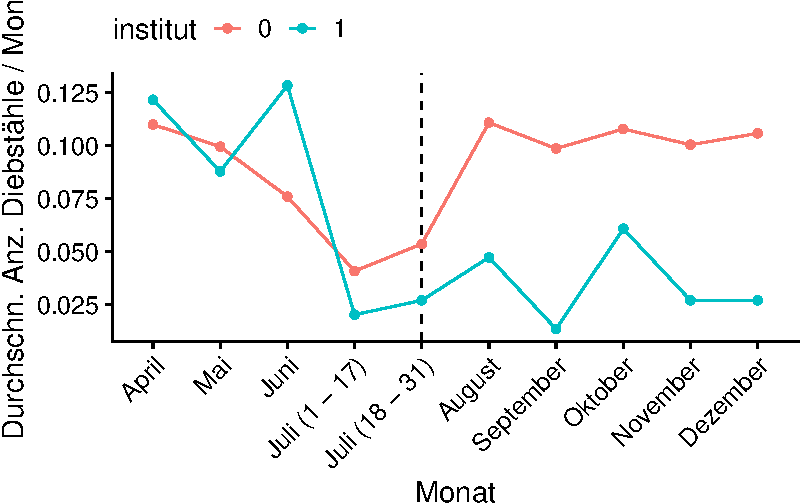
\includegraphics{DiD_files/figure-pdf/fig-totrobtrends-1.pdf}

}

\caption{\label{fig-totrobtrends}Geschätzte Trends für Autodiebstähle in
Buenos Aires im Jahr 1994}

\end{figure}%

Abbildung~\ref{fig-totrobtrends} zeigt einen ähnlichen Verlauf der
Trends für den Zeitraum unmittelbar vor dem Anschalg am 18. Juli.

Tabelle 2 in Di Tella und Schargrodsky (2004) präsentiert t-Tests für
Unterschiede in der Mittleren Anzahl der Diebstähle pro Monat zwischen
Blocks mit jüdischen Einrichtungen und verschiedenen distanz-basierten
Untergruppen von Blocks ohne eine jüdische Einrichtungen für jede
Periode. Zur Reproduktion dieser Ergebnisse erstellen zunächst eine
Listen-Spalten für die beobachteten Diebstähle in Abhängigkeit der
Distanz zum nächsten Block mit einer jüdischen Einrichtung.

\begin{itemize}
\tightlist
\item
  \texttt{d2more} Zwei oder mehr Blocks entfernt
\item
  \texttt{d2}: Zwei Blocks entfernt
\item
  \texttt{d1}: Ein Block entfernt
\item
  \texttt{same}: Jüdische Einrichtung im selben Block
\end{itemize}

\begin{Shaded}
\begin{Highlighting}[]
\NormalTok{(}
\NormalTok{  dat\_listcol }\OtherTok{\textless{}{-}}\NormalTok{ polizeipraesenz }\SpecialCharTok{\%\textgreater{}\%} 
    \FunctionTok{group\_by}\NormalTok{(observ, monat) }\SpecialCharTok{\%\textgreater{}\%}
    \FunctionTok{transmute}\NormalTok{(}
      \AttributeTok{d2more =} \FunctionTok{list}\NormalTok{(totrob[distanz }\SpecialCharTok{\textgreater{}} \DecValTok{2}\NormalTok{]),}
      \AttributeTok{d2 =} \FunctionTok{list}\NormalTok{(totrob[distanz }\SpecialCharTok{==} \DecValTok{2}\NormalTok{]),}
      \AttributeTok{d1 =} \FunctionTok{list}\NormalTok{(totrob[distanz }\SpecialCharTok{==} \DecValTok{1}\NormalTok{]),}
      \AttributeTok{same =} \FunctionTok{list}\NormalTok{(totrob[institut }\SpecialCharTok{==} \DecValTok{1}\NormalTok{])}
\NormalTok{    )}
\NormalTok{)}
\end{Highlighting}
\end{Shaded}

\begin{verbatim}
# A tibble: 8,760 x 6
# Groups:   observ, monat [8,760]
   observ monat d2more    d2        d1        same     
    <dbl> <ord> <list>    <list>    <list>    <list>   
 1    870 April <dbl [0]> <dbl [0]> <dbl [1]> <dbl [0]>
 2    851 April <dbl [0]> <dbl [1]> <dbl [0]> <dbl [0]>
 3    843 April <dbl [0]> <dbl [0]> <dbl [0]> <dbl [1]>
 4    796 April <dbl [0]> <dbl [0]> <dbl [1]> <dbl [0]>
 5    790 April <dbl [0]> <dbl [0]> <dbl [0]> <dbl [1]>
 6    789 April <dbl [0]> <dbl [0]> <dbl [1]> <dbl [0]>
 7    844 April <dbl [0]> <dbl [0]> <dbl [0]> <dbl [1]>
 8    858 April <dbl [0]> <dbl [0]> <dbl [1]> <dbl [0]>
 9    787 April <dbl [0]> <dbl [0]> <dbl [1]> <dbl [0]>
10    850 April <dbl [0]> <dbl [0]> <dbl [1]> <dbl [0]>
# i 8,750 more rows
\end{verbatim}

Mit \texttt{summarise()} können wir Stichprobenmittel und
Standardabweichungen der Diebstähle in Blocks dieser Kategorien für alle
Perioden berechnen. Anschließend kombinieren wir die Ergebnisse jeweils
mit \texttt{sprintf()} und formatieren das Ergebnis mit
\texttt{modelsummary::modelsummary\_df()}.\footnote{\texttt{"\%.4f\textbackslash{}n(\%.4f)"}
  gibt das Format des resultierenden \texttt{character} an: Mittelwerte
  und SDs (in Klammern), gerundet auf vier Nachkommastellen.
  \texttt{\textbackslash{}n} bewirkt einen Zeilenumbruch.}
Tabelle~\ref{tbl-deskstatdistanz} Zeit die Spalten A bis D aus Tabelle 2
in Di Tella und Schargrodsky (2004).

\begin{Shaded}
\begin{Highlighting}[]
\FunctionTok{library}\NormalTok{(modelsummary)}

\CommentTok{\# Mittelwerte und Standardabweichungen}
\NormalTok{mean\_sd }\OtherTok{\textless{}{-}}\NormalTok{ dat\_listcol }\SpecialCharTok{\%\textgreater{}\%}
  \FunctionTok{group\_by}\NormalTok{(monat) }\SpecialCharTok{\%\textgreater{}\%}
  \FunctionTok{summarise}\NormalTok{(}
    \FunctionTok{across}\NormalTok{(}
\NormalTok{      d2more}\SpecialCharTok{:}\NormalTok{same,}
      \AttributeTok{.fns =} \FunctionTok{list}\NormalTok{(}
        \AttributeTok{mean =} \SpecialCharTok{\textasciitilde{}} \FunctionTok{mean}\NormalTok{(}\FunctionTok{unlist}\NormalTok{(.)), }
        \AttributeTok{sd =} \SpecialCharTok{\textasciitilde{}} \FunctionTok{sd}\NormalTok{(}\FunctionTok{unlist}\NormalTok{(.))}
\NormalTok{      )}
\NormalTok{    ),}
    \AttributeTok{.groups =} \StringTok{"keep"}
\NormalTok{  )}

\CommentTok{\# Desk. Statistiken kombinieren}
\NormalTok{formatted\_mean\_sd }\OtherTok{\textless{}{-}}\NormalTok{ mean\_sd }\SpecialCharTok{\%\textgreater{}\%}
  \FunctionTok{transmute}\NormalTok{(}
\NormalTok{    monat,}
    \StringTok{"D\textgreater{}2 (A)"} \OtherTok{=} \FunctionTok{sprintf}\NormalTok{(}\StringTok{"\%.4f}\SpecialCharTok{\textbackslash{}n}\StringTok{(\%.4f)"}\NormalTok{, d2more\_mean, d2more\_sd),}
    \StringTok{"same (B)"} \OtherTok{=} \FunctionTok{sprintf}\NormalTok{(}\StringTok{"\%.4f}\SpecialCharTok{\textbackslash{}n}\StringTok{(\%.4f)"}\NormalTok{, same\_mean, same\_sd),}
    \StringTok{"D1 (C)"} \OtherTok{=} \FunctionTok{sprintf}\NormalTok{(}\StringTok{"\%.4f}\SpecialCharTok{\textbackslash{}n}\StringTok{(\%.4f)"}\NormalTok{, d1\_mean, d1\_sd),}
    \StringTok{"D2 (D)"} \OtherTok{=} \FunctionTok{sprintf}\NormalTok{(}\StringTok{"\%.4f}\SpecialCharTok{\textbackslash{}n}\StringTok{(\%.4f)"}\NormalTok{, d2\_mean, d2\_sd)}
\NormalTok{  )}

\CommentTok{\# Tabelle mit modelsummary\_df() ausgeben}
\NormalTok{modelsummary}\SpecialCharTok{::}\FunctionTok{datasummary\_df}\NormalTok{(formatted\_mean\_sd)}
\end{Highlighting}
\end{Shaded}

\begin{table}

\caption{\label{tbl-deskstatdistanz}Deskriptive Statistiken für
Diebstähle nach Entfernung zur nächsten jüdischen Einrichtung}

\centering{

\centering
\begin{tblr}[         %% tabularray outer open
]                     %% tabularray outer close
{                     %% tabularray inner open
colspec={Q[]Q[]Q[]Q[]Q[]},
column{1}={halign=l,},
column{2}={halign=l,},
column{3}={halign=l,},
column{4}={halign=l,},
column{5}={halign=l,},
}                     %% tabularray inner close
\toprule
monat & D>2 (A) & same (B) & D1 (C) & D2 (D) \\ \midrule %% TinyTableHeader
April          & 0.0996(0.2481) & 0.1216(0.3614) & 0.1211(0.2879) & 0.1228(0.2974) \\
Mai            & 0.1084(0.2357) & 0.0878(0.2060) & 0.0776(0.1817) & 0.0973(0.2591) \\
Juni           & 0.0785(0.1961) & 0.1284(0.2864) & 0.0776(0.2151) & 0.0697(0.1867) \\
Juli (1 - 17)  & 0.0393(0.1451) & 0.0203(0.0692) & 0.0590(0.2101) & 0.0310(0.1419) \\
Juli (18 - 31) & 0.0393(0.1460) & 0.0270(0.0787) & 0.0730(0.2177) & 0.0686(0.2386) \\
August         & 0.1184(0.2871) & 0.0473(0.1752) & 0.0668(0.2197) & 0.1272(0.3048) \\
September      & 0.1018(0.2566) & 0.0135(0.0573) & 0.0901(0.2761) & 0.0985(0.2483) \\
Oktober        & 0.1211(0.2671) & 0.0608(0.2157) & 0.0978(0.2610) & 0.0885(0.2367) \\
November       & 0.0962(0.2404) & 0.0270(0.0787) & 0.1102(0.2889) & 0.1018(0.2177) \\
Dezember       & 0.1018(0.2682) & 0.0270(0.0787) & 0.1165(0.2782) & 0.1062(0.2256) \\
\bottomrule
\end{tblr}

}

\end{table}%

Der nächste Chunk reproduziert die Spalten E bis F von Tabelle 2 in Di
Tella und Schargrodsky (2004). Die Einträge sind Mittelwertdifferenzen
(Standardfehler in Klammern) zwischen den betrachteten Gruppen von
Blocks sowie Ergebnisse für t-Tests (Signifikanz-Sternchen) der
Hypothese, dass die jeweilige mittlere Anzahl an Autodiebstählen nicht
verschieden ist.

Wir definieren zunächst eine Funktion \texttt{format\_ttest()}, die die
gewünschen Statistiken aus einem mit \texttt{t.test()} berechneten
Objekte ausliest und entsprechend formatiert. Anschließend nutzen wir
diese Funktion, um die Daten in \texttt{dat\_listcol} entsprechend der
Definition in Di Tella und Schargrodsky (2004) für jeden Monat
zusammenzufassen. Die Ergebnisse formatieren wir wieder mit
\texttt{datasummary\_df()}.

\begin{Shaded}
\begin{Highlighting}[]
\CommentTok{\# Funktion: Ergebnisse von t.test() }
\CommentTok{\# mit Signifikanzsternchen}
\NormalTok{format\_ttest }\OtherTok{\textless{}{-}} \ControlFlowTok{function}\NormalTok{(ttest\_result) \{}
\NormalTok{  estimate }\OtherTok{\textless{}{-}} \FunctionTok{diff}\NormalTok{(ttest\_result}\SpecialCharTok{$}\NormalTok{estimate)}
\NormalTok{  stderr }\OtherTok{\textless{}{-}}\NormalTok{ ttest\_result}\SpecialCharTok{$}\NormalTok{stderr}
\NormalTok{  p\_value }\OtherTok{\textless{}{-}}\NormalTok{ ttest\_result}\SpecialCharTok{$}\NormalTok{p.value}
  
\NormalTok{  stars }\OtherTok{\textless{}{-}} \ControlFlowTok{if}\NormalTok{ (p\_value }\SpecialCharTok{\textless{}} \FloatTok{0.001}\NormalTok{) \{}
    \StringTok{"***"}
\NormalTok{  \} }\ControlFlowTok{else} \ControlFlowTok{if}\NormalTok{ (p\_value }\SpecialCharTok{\textless{}} \FloatTok{0.01}\NormalTok{) \{}
    \StringTok{"**"}
\NormalTok{  \} }\ControlFlowTok{else} \ControlFlowTok{if}\NormalTok{ (p\_value }\SpecialCharTok{\textless{}} \FloatTok{0.05}\NormalTok{) \{}
    \StringTok{"*"}
\NormalTok{  \} }\ControlFlowTok{else}\NormalTok{ \{}
    \StringTok{""}
\NormalTok{  \}}
  
  \FunctionTok{sprintf}\NormalTok{(}\StringTok{"\%.4f (\%.4f)\%s"}\NormalTok{, estimate, stderr, stars)}
\NormalTok{\}}

\CommentTok{\# Berechnung der t{-}Tests, Formatierung der Ergebnisse}
\NormalTok{results }\OtherTok{\textless{}{-}}\NormalTok{ dat\_listcol }\SpecialCharTok{\%\textgreater{}\%}
  \FunctionTok{group\_by}\NormalTok{(monat) }\SpecialCharTok{\%\textgreater{}\%}
  \FunctionTok{summarise}\NormalTok{(}
    \StringTok{"(E) Diff: B {-} A"} \OtherTok{=} \FunctionTok{format\_ttest}\NormalTok{(}\FunctionTok{t.test}\NormalTok{(}\FunctionTok{unlist}\NormalTok{(d2more), }\FunctionTok{unlist}\NormalTok{(same))),}
    \StringTok{"(F) Diff: C {-} A"} \OtherTok{=} \FunctionTok{format\_ttest}\NormalTok{(}\FunctionTok{t.test}\NormalTok{(}\FunctionTok{unlist}\NormalTok{(d2more), }\FunctionTok{unlist}\NormalTok{(d1))),}
    \StringTok{"(G) Diff: D {-} A"} \OtherTok{=} \FunctionTok{format\_ttest}\NormalTok{(}\FunctionTok{t.test}\NormalTok{(}\FunctionTok{unlist}\NormalTok{(d2more), }\FunctionTok{unlist}\NormalTok{(d2)))}
\NormalTok{  )}

\CommentTok{\# Formatierung der Tabelle mit modelsummary\_df()}
\NormalTok{modelsummary}\SpecialCharTok{::}\FunctionTok{datasummary\_df}\NormalTok{(results)}
\end{Highlighting}
\end{Shaded}

\begin{table}

\caption{\label{tbl-ttestsdist}Mittelwertdifferenzen in Autodiebstählen
und t-Tests}

\centering{

\centering
\begin{tblr}[         %% tabularray outer open
]                     %% tabularray outer close
{                     %% tabularray inner open
colspec={Q[]Q[]Q[]Q[]},
column{1}={halign=l,},
column{2}={halign=l,},
column{3}={halign=l,},
column{4}={halign=l,},
}                     %% tabularray inner close
\toprule
monat & (E) Diff: B - A & (F) Diff: C - A & (G) Diff: D - A \\ \midrule %% TinyTableHeader
April          & 0.0221 (0.0606)     & 0.0216 (0.0255)   & 0.0232 (0.0230)  \\
Mai            & -0.0206 (0.0356)    & -0.0308 (0.0181)  & -0.0111 (0.0205) \\
Juni           & 0.0498 (0.0480)     & -0.0009 (0.0193)  & -0.0088 (0.0155) \\
Juli (1 - 17)  & -0.0190 (0.0133)    & 0.0197 (0.0179)   & -0.0083 (0.0116) \\
Juli (18 - 31) & -0.0122 (0.0146)    & 0.0337 (0.0185)   & 0.0293 (0.0173)  \\
August         & -0.0711 (0.0318)*   & -0.0516 (0.0220)* & 0.0088 (0.0244)  \\
September      & -0.0883 (0.0153)*** & -0.0117 (0.0249)  & -0.0033 (0.0205) \\
Oktober        & -0.0603 (0.0376)    & -0.0233 (0.0241)  & -0.0326 (0.0201) \\
November       & -0.0692 (0.0172)*** & 0.0140 (0.0254)   & 0.0055 (0.0184)  \\
Dezember       & -0.0747 (0.0181)*** & 0.0147 (0.0253)   & 0.0044 (0.0196)  \\
\bottomrule
\end{tblr}

}

\end{table}%

Tabelle~\ref{tbl-ttestsdist} zeigt eine einschlägige Entwicklung der
Differenzen über die Zeit: In den Monaten \emph{vor} dem Anschlag (und
der anschließenden Allokation von Polizeipräsenz) bestehen weder
zwischen weit entfernten Blocks und solchen mit einer jüdischen
Einrichtung (Spalte E) noch zwischen Blocks ohne eine Einrichtung
(Spalten F und G) signifikante unterschiede in der Anzahl der
Autodiebstähle. \emph{Nach} der politischen Intervention ergibt sich ein
anderes Bild: In Spalte (E) von Tabelle~\ref{tbl-ttestsdist} finden wir
signifikante \emph{negative} Differenzen. Dies ist Evidenz, das die
Kriminalität in besonders gut bewachten Blocks (Spalte B in
Tabelle~\ref{tbl-deskstatdistanz}) in den Folgeperioden des Anschlags
geringer war als in Blocks die, mehr als zwei Blocks von einer
bewachteten Einrichtung entfernt sind (Spalte A in
Tabelle~\ref{tbl-deskstatdistanz}). Mit Ausnahme einer Signifikanten
Differenz im August 1994 finden wir keine Hinweise auf derartige
Unterschiede zwischen Blocks in den Kontrollgruppen (Spalten F und G).

\subsection{Two-Way-Fixed-Effects-Schätzungen}\label{two-way-fixed-effects-schuxe4tzungen}

Di Tella und Schargrodsky (2004) betrachten (Sub-Modelle) der folgenden
Regressionsspezifikation für die Schätzung des Effekts von
Polizeipräsenz auf die Anzahl der Autodiebstähle.

\begin{align}
  \begin{split}
  \text{totrob}_{i,t} =&\, \text{monat}_t + \text{block}_i \\
  + &\, \alpha_0 \text{same}_{i,t} + \alpha_1 \text{oneblock}_{i,t} \\
  + &\, \alpha_2 \text{twoblocks}_{i,t} + \epsilon_{i,t}
  \end{split}\label{eq:ppbase}
\end{align}

Hierbei sind \(\text{monat}_t\) und \(\text{block}_i\) Fixed Effekte für
den Monat sowie den Block. Die übrigen Variablen sind für Beobachtungen
ab dem Anschlag am 18. Juli 1994 und in Abhäbgigkeit der Distanz zur
nächsten jüdischen Einrichtnug definiert:

\begin{itemize}
\item
  \(\text{same}_{i,t}\): Dummy-Variable für jüdische Einrichtung im
  Block und Beobachtung nach dem 17. Juli 1994
\item
  \(\text{oneblock}_{i,t}\): Dummy-Variable für Blocks mit einem Block
  Entfernung zum nächsten Block mit einer jüdischen Einrichtung und
  Beobachtung nach dem 17. Juli 1994
\item
  \(\text{twoblocks}_{i,t}\): Dummy-Variable für Blocks mit einer
  Entfernung von zwei Blocks zum nächsten Block mit einer jüdischen
  Einrichtung und Beobachtung nach dem 17. Juli 1994
\end{itemize}

Im nächsten Code-Chunk definieren wir diese Variablen und, gemäß der
Vorgehensweise in Di Tella und Schargrodsky (2004), entfernen
Beobachtungen für den Zeitraum im Juli nach dem Anschlag (18.07.1994 bis
31.07.1994).

\begin{Shaded}
\begin{Highlighting}[]
\CommentTok{\# Variablen definieren und Beobachtungen subsetten}
\NormalTok{dat\_DID }\OtherTok{\textless{}{-}}\NormalTok{ polizeipraesenz }\SpecialCharTok{\%\textgreater{}\%}
  \FunctionTok{mutate}\NormalTok{(}
    \AttributeTok{same =}\NormalTok{ institut }\SpecialCharTok{==} \DecValTok{1} \SpecialCharTok{\&}\NormalTok{ monat }\SpecialCharTok{\textgreater{}} \StringTok{"Juli (1 {-} 17)"}\NormalTok{,}
    \AttributeTok{oneblock =}\NormalTok{ distanz }\SpecialCharTok{==} \DecValTok{1} \SpecialCharTok{\&}\NormalTok{  monat }\SpecialCharTok{\textgreater{}} \StringTok{"Juli (1 {-} 17)"}\NormalTok{,}
    \AttributeTok{twoblocks =}\NormalTok{ distanz }\SpecialCharTok{==} \DecValTok{2} \SpecialCharTok{\&}\NormalTok{  monat }\SpecialCharTok{\textgreater{}} \StringTok{"Juli (1 {-} 17)"}
\NormalTok{  ) }\SpecialCharTok{\%\textgreater{}\%} 
  \FunctionTok{filter}\NormalTok{(monat }\SpecialCharTok{!=} \StringTok{"Juli (18 {-} 31)"}\NormalTok{)}
\end{Highlighting}
\end{Shaded}

Die Kernergebnisse der Studie werden in Tabelle 3 im Paper präsentiert.
Hier werden fünf Regressionen betrachtet:

\begin{itemize}
\item
  \textbf{Regression (A)}

  \begin{align}
      \begin{split}
        \text{totrob}_{i,t} 
          =&\, \text{monat}_t + \text{block}_i \\
         + &\, \alpha_0 \text{same}_{i,t} \\
         + &\, \epsilon_{i,t}
      \end{split}\label{eq:ppbaseA}
  \end{align}

  Modell \eqref{eq:ppbaseA} betrachtet lediglich die geographisch
  ``engste'' Definition des Behandlungseffekts: \(\alpha_0\) ist der ATT
  für Blocks mit einer jüdischen Einrichtung. Die Kontrollgruppe besteht
  aus \emph{sämtlichen} Blocks ohne jüdische Einrichtung.
\item
  \textbf{Regression (B)}

  \begin{align}
      \begin{split}
        \text{totrob}_{i,t} 
          =&\, \text{monat}_t + \text{block}_i \\
         + &\, \alpha_0 \text{same}_{i,t} \\
         + &\, \alpha_1 \text{oneblock}_{i,t} \\
         + &\, \epsilon_{i,t}
      \end{split}\label{eq:ppbaseB}
  \end{align}

  Modell \eqref{eq:ppbaseB} erweitert die Behandlungsgruppe um Blocks,
  die genau einen Block von einem Block mit erhötem Polizeischutz
  entfernt sind. Die Kontrollgruppe besteht aus Blocks mit einer
  Entfernung von \emph{zwei oder mehr Blocks} bis zur nächsten jüdischen
  Einrichtung.
\item
  \textbf{Regression (C)}

  \begin{align}
      \begin{split}
        \text{totrob}_{i,t} 
          =&\, \text{monat}_t + \text{block}_i \\
         + &\, \alpha_0 \text{same}_{i,t} \\
         + &\, \alpha_1 \text{oneblock}_{i,t} \\
         + &\, \alpha_1 \text{twoblocks}_{i,t} \\
         + &\, \epsilon_{i,t}
      \end{split}\label{eq:ppbaseC}
  \end{align}

  Modell \eqref{eq:ppbaseC} betrachtet zusätzlich den Behandlungseffekt
  in Blocks mit zwei Blocks entfernung zu einem Block mir erhöhter
  Polizeipräsenz. Die Kontrollgruppe besteht aus Blocks mit einer
  Entfernung von \emph{mehr als zwei Blocks} bis zur nächsten jüdischen
  Einrichtung.
\item
  \textbf{Regression (D) -- Querschnitts-Variation}

  Da Di Tella und Schargrodsky (2004) eine große Ähnlichkeit
  hinsichtlich demografischer Merkmale und Autodiebstahlsraten vor der
  Intervention in Gebieten mit und ohne jüdische Einrichtungen
  beobachten, betrachten sie auch einen einfachen Querschnittsschätzer.
  Regression (D) nutzt die Spezifikation \eqref{eq:ppbaseC}, aber
  berücksichtigt nur Beobachtungen für den Zeitraum nach dem Anschlag
  (August bis Dezember) und nutzt lediglich Fixed Effekts für die
  \emph{Monate}.
\item
  \textbf{Regression (E) -- Zeitreihen-Variation}

  Regression (E) ist eine alternative Spezifikation zu
  \eqref{eq:ppbaseC} bei der lediglich die zeitliche Variation in der
  Behandlungsgruppe (Entfernung zur nächsten Einrichtung \(\leq\) zwei
  Blocks) genutzt wird. Hierzu werden Fixed Effekts nur für die
  \emph{Blocks}, jedoch nicht für die Monate berechnet.
\end{itemize}

Wie implementieren nachfolgend die Regressionen (A) bis (E) mit
\texttt{fixest::feols()} unter Verwendung heteroskedastie-robuster
Standardfehler (\texttt{vcov\ =\ "HC1"}). Alle Regressionen nutzen den
oben definierten Datensatz \texttt{dat\_DID}, wobei wir für die
Schätzungen in (D) und (E) mit \texttt{filter()} die entsprechenden
Subsets auswählen.

\begin{Shaded}
\begin{Highlighting}[]
\CommentTok{\# Regression (A)}
\NormalTok{(}
\NormalTok{  T3A }\OtherTok{\textless{}{-}} \FunctionTok{feols}\NormalTok{(}
    \AttributeTok{fml =}\NormalTok{ totrob }\SpecialCharTok{\textasciitilde{}} 
\NormalTok{      same}
    \SpecialCharTok{|}\NormalTok{ observ }\SpecialCharTok{+}\NormalTok{ monat, }
    \AttributeTok{data =}\NormalTok{ dat\_DID, }
    \AttributeTok{vcov =} \StringTok{"HC1"}
\NormalTok{  )}
\NormalTok{)}
\end{Highlighting}
\end{Shaded}

\begin{verbatim}
OLS estimation, Dep. Var.: totrob
Observations: 7,884
Fixed-effects: observ: 876,  monat: 9
Standard-errors: Heteroskedasticity-robust 
         Estimate Std. Error t value   Pr(>|t|)    
sameTRUE -0.07753    0.02244  -3.456 0.00055241 ***
---
Signif. codes:  0 '***' 0.001 '**' 0.01 '*' 0.05 '.' 0.1 ' ' 1
RMSE: 0.216676     Adj. R2: 0.097072
                 Within R2: 0.001277
\end{verbatim}

\begin{Shaded}
\begin{Highlighting}[]
\CommentTok{\# Regression (B)}
\NormalTok{(}
\NormalTok{  T3B }\OtherTok{\textless{}{-}} \FunctionTok{feols}\NormalTok{(}
    \AttributeTok{fml =}\NormalTok{ totrob }\SpecialCharTok{\textasciitilde{}} 
\NormalTok{      same  }
    \SpecialCharTok{+}\NormalTok{ oneblock }
    \SpecialCharTok{|}\NormalTok{ observ }\SpecialCharTok{+}\NormalTok{ monat, }
    \AttributeTok{data =}\NormalTok{ dat\_DID, }
    \AttributeTok{vcov =} \StringTok{"HC1"}
\NormalTok{  )}
\NormalTok{)}
\end{Highlighting}
\end{Shaded}

\begin{verbatim}
OLS estimation, Dep. Var.: totrob
Observations: 7,884
Fixed-effects: observ: 876,  monat: 9
Standard-errors: Heteroskedasticity-robust 
             Estimate Std. Error t value   Pr(>|t|)    
sameTRUE     -0.08007    0.02257 -3.5480 0.00039068 ***
oneblockTRUE -0.01326    0.01386 -0.9564 0.33889333    
---
Signif. codes:  0 '***' 0.001 '**' 0.01 '*' 0.05 '.' 0.1 ' ' 1
RMSE: 0.216661     Adj. R2: 0.097067
                 Within R2: 0.001414
\end{verbatim}

\begin{Shaded}
\begin{Highlighting}[]
\CommentTok{\# Regression (C)}
\NormalTok{(}
\NormalTok{  T3C }\OtherTok{\textless{}{-}} \FunctionTok{feols}\NormalTok{(}
    \AttributeTok{fml =}\NormalTok{ totrob }\SpecialCharTok{\textasciitilde{}} 
\NormalTok{      same}
    \SpecialCharTok{+}\NormalTok{ oneblock }
    \SpecialCharTok{+}\NormalTok{ twoblocks }
    \SpecialCharTok{|}\NormalTok{ observ }\SpecialCharTok{+}\NormalTok{ monat, }
    \AttributeTok{data =}\NormalTok{ dat\_DID, }
    \AttributeTok{vcov =} \StringTok{"HC1"}
\NormalTok{  )}
\NormalTok{)}
\end{Highlighting}
\end{Shaded}

\begin{verbatim}
OLS estimation, Dep. Var.: totrob
Observations: 7,884
Fixed-effects: observ: 876,  monat: 9
Standard-errors: Heteroskedasticity-robust 
               Estimate Std. Error t value   Pr(>|t|)    
sameTRUE      -0.080802    0.02295 -3.5216 0.00043173 ***
oneblockTRUE  -0.013988    0.01447 -0.9669 0.33362749    
twoblocksTRUE -0.002185    0.01232 -0.1774 0.85920503    
---
Signif. codes:  0 '***' 0.001 '**' 0.01 '*' 0.05 '.' 0.1 ' ' 1
RMSE: 0.21666     Adj. R2: 0.096942
                Within R2: 0.001419
\end{verbatim}

\begin{Shaded}
\begin{Highlighting}[]
\CommentTok{\# Regression (D)}
\NormalTok{(}
\NormalTok{  T3D }\OtherTok{\textless{}{-}} \FunctionTok{feols}\NormalTok{(}
    \AttributeTok{fml =}\NormalTok{ totrob }\SpecialCharTok{\textasciitilde{}} 
\NormalTok{      same}
    \SpecialCharTok{+}\NormalTok{ oneblock}
    \SpecialCharTok{+}\NormalTok{ twoblocks }
    \SpecialCharTok{|}\NormalTok{ monat,}
    \AttributeTok{data =}\NormalTok{ dat\_DID }\SpecialCharTok{\%\textgreater{}\%} 
      \FunctionTok{filter}\NormalTok{(}
\NormalTok{        monat }\SpecialCharTok{\textgreater{}=} \StringTok{"August"}
\NormalTok{      ),}
    \AttributeTok{vcov =} \StringTok{"HC1"}
\NormalTok{  )}
\NormalTok{)}
\end{Highlighting}
\end{Shaded}

\begin{verbatim}
OLS estimation, Dep. Var.: totrob
Observations: 4,380
Fixed-effects: monat: 5
Standard-errors: Heteroskedasticity-robust 
               Estimate Std. Error t value   Pr(>|t|)    
sameTRUE      -0.072719    0.01139 -6.3852 1.8897e-10 ***
oneblockTRUE  -0.011581    0.01090 -1.0623 2.8815e-01    
twoblocksTRUE -0.003429    0.00925 -0.3707 7.1086e-01    
---
Signif. codes:  0 '***' 0.001 '**' 0.01 '*' 0.05 '.' 0.1 ' ' 1
RMSE: 0.256214     Adj. R2: 0.002028
                 Within R2: 0.00325 
\end{verbatim}

\begin{Shaded}
\begin{Highlighting}[]
\CommentTok{\# Regression (E)}
\NormalTok{(}
\NormalTok{  T3E }\OtherTok{\textless{}{-}} \FunctionTok{feols}\NormalTok{(}
    \AttributeTok{fml =}\NormalTok{ totrob }\SpecialCharTok{\textasciitilde{}}
\NormalTok{      same }
    \SpecialCharTok{+}\NormalTok{ oneblock }
    \SpecialCharTok{+}\NormalTok{ twoblocks }
    \SpecialCharTok{|}\NormalTok{ observ,}
    \AttributeTok{data =}\NormalTok{ dat\_DID }\SpecialCharTok{\%\textgreater{}\%} 
      \FunctionTok{filter}\NormalTok{(}
\NormalTok{        distanz }\SpecialCharTok{\textless{}=} \DecValTok{2}
\NormalTok{      ), }
    \AttributeTok{vcov =} \StringTok{"HC1"}
\NormalTok{  )}
\NormalTok{)}
\end{Highlighting}
\end{Shaded}

\begin{verbatim}
OLS estimation, Dep. Var.: totrob
Observations: 3,816
Fixed-effects: observ: 424
Standard-errors: Heteroskedasticity-robust 
              Estimate Std. Error t value Pr(>|t|)    
sameTRUE      -0.05439    0.02201 -2.4713 0.013510 *  
oneblockTRUE   0.01242    0.01260  0.9861 0.324146    
twoblocksTRUE  0.02423    0.01011  2.3972 0.016577 *  
---
Signif. codes:  0 '***' 0.001 '**' 0.01 '*' 0.05 '.' 0.1 ' ' 1
RMSE: 0.216568     Adj. R2: 0.093304
                 Within R2: 0.003304
\end{verbatim}

Zur Reproduktion von Tabelle 3 in Di Tella und Schargrodsky (2004)
sammeln wir die geschätzten Modelle und erzeugen einen tabelarrische
Zusammenfassung mit \texttt{modelsummary::modelsummary()}. Über das
Argument
\texttt{gof\_omit\ =\ "\^{}(?!(R2\textbar{}Num.Obs.\textbar{}FE.*)\$).*"}
wählen wir unter den Goodness-of-Fit-Statistiken \(R^2\), die Anzahl der
Beobachtungen, sowie Indikatoren für die verwendeten Fixed Effekts mit
einem \href{https://de.wikipedia.org/wiki/Regulärer_Ausdruck}{Regular
Expression} aus.\footnote{Der Ausdruck
  \texttt{\^{}(?!(R2\textbar{}Num.Obs.\textbar{}FE.*)\$).*} matcht jede
  Zeichenkette, außer sie ist ``R2'', ``Num.Obs.'' oder beginnt mit
  ``FE''. Andere Statistiken als diese Matches werden also in der
  Tabelle ausgelassen.}

\begin{Shaded}
\begin{Highlighting}[]
\CommentTok{\# Tabellarischer Vergleich mit modelsummary()}
\CommentTok{\# (Tabelle 3 in Ditella und Schargrodsky, 2004)}
\FunctionTok{modelsummary}\NormalTok{(}
  \AttributeTok{models =} \FunctionTok{list}\NormalTok{(}
    \StringTok{"(3A)"} \OtherTok{=}\NormalTok{ T3A, }
    \StringTok{"(3B)"} \OtherTok{=}\NormalTok{ T3B, }
    \StringTok{"(3C)"} \OtherTok{=}\NormalTok{ T3C, }
    \StringTok{"(3D)"} \OtherTok{=}\NormalTok{ T3D, }
    \StringTok{"(3E)"} \OtherTok{=}\NormalTok{ T3E}
\NormalTok{  ),}
  \AttributeTok{stars =}\NormalTok{ T,}
  \AttributeTok{gof\_omit =} \StringTok{"\^{}(?!(R2|Num.Obs.|FE.*)$).*"}\NormalTok{, }
  \AttributeTok{output =} \StringTok{"gt"}
\NormalTok{)}
\end{Highlighting}
\end{Shaded}

\setlength{\LTpost}{0mm}

\begin{longtable}{lccccc}

\caption{\label{tbl-ditella3}Schätzungen des Effekts von Polizeipräsenz
auf Autodiebstähle}

\tabularnewline

\toprule
  & (3A) & (3B) & (3C) & (3D) & (3E) \\ 
\midrule\addlinespace[2.5pt]
sameTRUE & -0.078*** & -0.080*** & -0.081*** & -0.073*** & -0.054* \\ 
 & (0.022) & (0.023) & (0.023) & (0.011) & (0.022) \\ 
oneblockTRUE &  & -0.013 & -0.014 & -0.012 & 0.012 \\ 
 &  & (0.014) & (0.014) & (0.011) & (0.013) \\ 
twoblocksTRUE &  &  & -0.002 & -0.003 & 0.024* \\ 
 &  &  & (0.012) & (0.009) & (0.010) \\ 
Num.Obs. & 7884 & 7884 & 7884 & 4380 & 3816 \\ 
R2 & 0.198 & 0.198 & 0.198 & 0.004 & 0.195 \\ 
FE: observ & X & X & X &  & X \\ 
FE: monat & X & X & X & X &  \\ 
\bottomrule

\end{longtable}

\begin{minipage}{\linewidth}
+ p < 0.1, * p < 0.05, ** p < 0.01, *** p < 0.001\\
\end{minipage}

Tabelle~\ref{tbl-ditella3} präsentiert die Ergebnisse. Der Koeffizient
von \texttt{same} ist jeweils in den Regressionen (3A), (3B) und (3C)
negativ und hoch-signifikant. Die Stärke des geschätzten Effekt (und der
Standardfehler) unterscheidet sich kaum zwischen den Modellen. Weiterhin
sind die Koeffizienten von \texttt{oneblock} und \texttt{twoblocks}
jeweils nicht signifikant von null verschieden. Die Interpretation
dieser Ergebnisse ist, dass es einen lokal-beschränkten Effekt der
erhöhten Polizeipräsenz auf Autodiebstähle in Blocks mit Polizeischutz
gab: Die Polizeipräsenz verringerte die durchschnittliche Anzahl der
Diebstähle in diesen Blocks um etwa \(.08\) Diebstähle pro Monat.

Die Ergebnisse für die Modelle (3D) und (3E) zeigen ebenfalls
signifikante negative Effekte des Polizeischutz anhand von Querschnitts-
und Zeitreihenvariation und untermauern damit die Robustheit des
gewählten Forschungsdesigns.

Zur besseren Interpretation des geschätzten Effekt in Modell (C)
vergleichen wir mit der durchschnittlichen Anzahl der Diebstähle pro
Monat in der Kontrollgruppe (Blocks mit einer Entfernung von mehr als
zwei Blocks zum nächsten geschützten Block) für den Zeitraum von August
1994 bis Dezember 1994:\footnote{Wir berechnen also
  \(\widehat{\alpha}_0 / \overline{\text{Diebstahlrate}} \cdot 100\).}

\begin{Shaded}
\begin{Highlighting}[]
\CommentTok{\# Vergl. Effekt mit durchschnittlicher Anz. Diebstähle }
\CommentTok{\# in der Kontrollgruppe}
\NormalTok{( }
  \CommentTok{\# gesch. Effekt}
\NormalTok{  T3C }\SpecialCharTok{\%\textgreater{}\%} 
    \FunctionTok{coefficients}\NormalTok{() }\SpecialCharTok{\%\textgreater{}\%} 
\NormalTok{    .[}\StringTok{"sameTRUE"}\NormalTok{] }
\NormalTok{) }\SpecialCharTok{/} 
\NormalTok{  ( }\CommentTok{\# Durchschnittt}
\NormalTok{    polizeipraesenz }\SpecialCharTok{\%\textgreater{}\%} 
      \FunctionTok{filter}\NormalTok{(}
\NormalTok{        monat }\SpecialCharTok{\textgreater{}=} \StringTok{"August"} \SpecialCharTok{\&}\NormalTok{ monat }\SpecialCharTok{\textless{}=} \StringTok{"Dezember"}\NormalTok{,}
\NormalTok{        distanz }\SpecialCharTok{\textgreater{}} \DecValTok{2}
\NormalTok{      ) }\SpecialCharTok{\%\textgreater{}\%}
      \FunctionTok{summarise}\NormalTok{(}
        \AttributeTok{m\_totrob =} \FunctionTok{mean}\NormalTok{(totrob)}
\NormalTok{      ) }\SpecialCharTok{\%\textgreater{}\%} 
      \FunctionTok{pull}\NormalTok{(m\_totrob)}
\NormalTok{  ) }\SpecialCharTok{*} \DecValTok{100}
\end{Highlighting}
\end{Shaded}

\begin{verbatim}
sameTRUE 
  -74.92 
\end{verbatim}

Die Rechnung zeigt, dass es in dem betrachten Zeitraum durch die
Behandlung mit zusätzlicher Polizeipräsenz zu einem Rückgang der Anzahl
an Autodiebstählen um durchschnittlich \(75\%\) in Blocks mit jüdischen
Einrichtungen kam.

\subsection{Placebo-Tests}\label{placebo-tests}

Placebo-Tests sind nützlich, um zu überprüfen, ob der geschätzte
Zusammenhang zwischen der Erhöhung der Polizeipräsenz und der
Verringerung der Kriminalität tatsächlich kausal ist oder ob andere
Faktoren eine Rolle spielen. Ein möglicher Einfluss könnte
beispielsweise durch zufällige temporäre Schwankungen in den
Kriminalitätsraten entstehen. Di Tella und Schargrodsky (2004)
wiederholen hierzu die Analyse anhand der Spezifikationen (3A), (3B) und
(3C) für fiktive Interventionszeitpunkte \emph{vor dem Anschlag}.
Hierbei werden Ende April (4A), Ende Mai (4B) und Ende Juni (4C) als
fiktive Zeitpunkte für die Placebo-Behandlung gewählt. Wenn diese
Placebo-Tests ähnliche Ergebnisse (signifikante negative Schätzungen)
wie die ursprüngliche Untersuchung liefern, könnte dies darauf
hindeuten, dass die in Tabelle~\ref{tbl-ditella3} geschätzten Effekte
nicht kausal sind.

Wir replizieren diese Ergebnisse, indem wir die Schätzungen von (3A),
(3B) und (3C) mit entsprechender Definition des Behandlungsindikators
(\texttt{group}) jeweils für modifizierte Datensätze mit sämtlichen
\(3504\) Beobachtungen vor dem Anschlag
(\texttt{filter(monat\ \textless{}=\ "Juli\ (1\ -\ 17)")}) wiederholen.

\begin{Shaded}
\begin{Highlighting}[]
\CommentTok{\# (4A)}
\CommentTok{\# Placebo{-}Schätzung für }
\NormalTok{dat\_T4A }\OtherTok{\textless{}{-}}\NormalTok{ polizeipraesenz }\SpecialCharTok{\%\textgreater{}\%}
  \FunctionTok{mutate}\NormalTok{(}
    \AttributeTok{group =}\NormalTok{ monat }\SpecialCharTok{\textgreater{}=} \StringTok{"Mai"} \SpecialCharTok{\&}\NormalTok{ monat }\SpecialCharTok{\textless{}=} \StringTok{"Juli (1 {-} 17)"}\NormalTok{,}
    \AttributeTok{same =}\NormalTok{ (institut }\SpecialCharTok{==} \DecValTok{1}\NormalTok{) }\SpecialCharTok{*}\NormalTok{ group,}
    \AttributeTok{oneblock =}\NormalTok{ (distanz }\SpecialCharTok{==} \DecValTok{1}\NormalTok{) }\SpecialCharTok{*}\NormalTok{ group,}
    \AttributeTok{twoblocks =}\NormalTok{ (distanz }\SpecialCharTok{==} \DecValTok{2}\NormalTok{) }\SpecialCharTok{*}\NormalTok{ group}
\NormalTok{  ) }\SpecialCharTok{\%\textgreater{}\%} 
  \FunctionTok{filter}\NormalTok{(monat }\SpecialCharTok{\textless{}=} \StringTok{"Juli (1 {-} 17)"}\NormalTok{)}

\NormalTok{(}
\NormalTok{  T4A }\OtherTok{\textless{}{-}} \FunctionTok{feols}\NormalTok{(}
    \AttributeTok{fml =}\NormalTok{ totrob }\SpecialCharTok{\textasciitilde{}} 
\NormalTok{      same }\SpecialCharTok{+}
\NormalTok{      oneblock }\SpecialCharTok{+}
\NormalTok{      twoblocks }
    \SpecialCharTok{|}\NormalTok{ observ }\SpecialCharTok{+}\NormalTok{ monat, }
    \AttributeTok{data =}\NormalTok{ dat\_T4A, }
    \AttributeTok{vcov =} \StringTok{"HC1"}
\NormalTok{  )}
\NormalTok{)}
\end{Highlighting}
\end{Shaded}

\begin{verbatim}
OLS estimation, Dep. Var.: totrob
Observations: 3,504
Fixed-effects: observ: 876,  monat: 4
Standard-errors: Heteroskedasticity-robust 
          Estimate Std. Error t value Pr(>|t|) 
same      -0.01864    0.05323 -0.3502  0.72622 
oneblock  -0.02554    0.02519 -1.0138  0.31075 
twoblocks -0.03263    0.02264 -1.4410  0.14969 
---
Signif. codes:  0 '***' 0.001 '**' 0.01 '*' 0.05 '.' 0.1 ' ' 1
RMSE: 0.18282     Adj. R2: 0.092254
                Within R2: 0.001211
\end{verbatim}

\begin{Shaded}
\begin{Highlighting}[]
\CommentTok{\# (4B)}
\NormalTok{dat\_T4B }\OtherTok{\textless{}{-}}\NormalTok{ dat\_T4A }\SpecialCharTok{\%\textgreater{}\%}
  \FunctionTok{mutate}\NormalTok{(}
    \AttributeTok{group =}\NormalTok{ monat }\SpecialCharTok{\textgreater{}=} \StringTok{"Juni"} \SpecialCharTok{\&}\NormalTok{ monat }\SpecialCharTok{\textless{}=} \StringTok{"Juli (1 {-} 17)"}\NormalTok{,}
    \AttributeTok{same =}\NormalTok{ (institut }\SpecialCharTok{==} \DecValTok{1}\NormalTok{) }\SpecialCharTok{*}\NormalTok{ group,}
    \AttributeTok{oneblock =}\NormalTok{ (distanz }\SpecialCharTok{==} \DecValTok{1}\NormalTok{) }\SpecialCharTok{*}\NormalTok{ group,}
    \AttributeTok{twoblocks =}\NormalTok{ (distanz }\SpecialCharTok{==} \DecValTok{2}\NormalTok{) }\SpecialCharTok{*}\NormalTok{ group}
\NormalTok{  ) }

\NormalTok{(}
\NormalTok{  T4B }\OtherTok{\textless{}{-}} \FunctionTok{feols}\NormalTok{(}
    \AttributeTok{fml =}\NormalTok{ totrob }\SpecialCharTok{\textasciitilde{}} 
\NormalTok{      same}
    \SpecialCharTok{+}\NormalTok{ oneblock}
    \SpecialCharTok{+}\NormalTok{ twoblocks }
    \SpecialCharTok{|}\NormalTok{ observ }\SpecialCharTok{+}\NormalTok{ monat, }
    \AttributeTok{data =}\NormalTok{ dat\_T4B, }
    \AttributeTok{vcov =} \StringTok{"HC1"}
\NormalTok{  )}
\NormalTok{)}
\end{Highlighting}
\end{Shaded}

\begin{verbatim}
OLS estimation, Dep. Var.: totrob
Observations: 3,504
Fixed-effects: observ: 876,  monat: 4
Standard-errors: Heteroskedasticity-robust 
          Estimate Std. Error t value Pr(>|t|) 
same       0.01467    0.04011  0.3658  0.71451 
oneblock   0.01402    0.01976  0.7096  0.47799 
twoblocks -0.01466    0.01736 -0.8443  0.39856 
---
Signif. codes:  0 '***' 0.001 '**' 0.01 '*' 0.05 '.' 0.1 ' ' 1
RMSE: 0.182863     Adj. R2: 0.091835
                 Within R2: 7.494e-4
\end{verbatim}

\begin{Shaded}
\begin{Highlighting}[]
\CommentTok{\# (4C)}
\NormalTok{dat\_T4C }\OtherTok{\textless{}{-}}\NormalTok{ dat\_T4A }\SpecialCharTok{\%\textgreater{}\%}
  \FunctionTok{mutate}\NormalTok{(}
    \AttributeTok{group =}\NormalTok{ monat }\SpecialCharTok{\%in\%} \FunctionTok{c}\NormalTok{(}\StringTok{"Juli (1 {-} 17)"}\NormalTok{),}
    \AttributeTok{same =}\NormalTok{ (institut }\SpecialCharTok{==} \DecValTok{1}\NormalTok{) }\SpecialCharTok{*}\NormalTok{ group,}
    \AttributeTok{oneblock =}\NormalTok{ (distanz }\SpecialCharTok{==} \DecValTok{1}\NormalTok{) }\SpecialCharTok{*}\NormalTok{ group,}
    \AttributeTok{twoblocks =}\NormalTok{ (distanz }\SpecialCharTok{==} \DecValTok{2}\NormalTok{) }\SpecialCharTok{*}\NormalTok{ group}
\NormalTok{  ) }

\NormalTok{(}
\NormalTok{  T4C }\OtherTok{\textless{}{-}} \FunctionTok{feols}\NormalTok{(}
    \AttributeTok{fml =}\NormalTok{ totrob }\SpecialCharTok{\textasciitilde{}} 
\NormalTok{      same}
    \SpecialCharTok{+}\NormalTok{ oneblock}
    \SpecialCharTok{+}\NormalTok{ twoblocks}
    \SpecialCharTok{|}\NormalTok{ observ }\SpecialCharTok{+}\NormalTok{ monat, }
    \AttributeTok{data =}\NormalTok{ dat\_T4C, }
    \AttributeTok{vcov =} \StringTok{"HC1"}
\NormalTok{  )}
\NormalTok{)}
\end{Highlighting}
\end{Shaded}

\begin{verbatim}
OLS estimation, Dep. Var.: totrob
Observations: 3,504
Fixed-effects: observ: 876,  monat: 4
Standard-errors: Heteroskedasticity-robust 
           Estimate Std. Error t value Pr(>|t|) 
same      -0.036111    0.03858 -0.9361  0.34933 
oneblock   0.023105    0.02245  1.0294  0.30340 
twoblocks -0.009403    0.01693 -0.5554  0.57870 
---
Signif. codes:  0 '***' 0.001 '**' 0.01 '*' 0.05 '.' 0.1 ' ' 1
RMSE: 0.182841     Adj. R2: 0.09205 
                 Within R2: 9.857e-4
\end{verbatim}

\begin{Shaded}
\begin{Highlighting}[]
\CommentTok{\# Tabellarische Zusamenfassung mit modelsummary()}
\CommentTok{\# (Tabelle 4 in Ditella und Schargrodsky, 2004)}
\FunctionTok{modelsummary}\NormalTok{(}
  \AttributeTok{models =} \FunctionTok{list}\NormalTok{(}
    \StringTok{"(4A)"} \OtherTok{=}\NormalTok{ T4A,}
    \StringTok{"(4B)"} \OtherTok{=}\NormalTok{ T4B,}
    \StringTok{"(4C)"} \OtherTok{=}\NormalTok{ T4C}
\NormalTok{  ), }
  \AttributeTok{stars =}\NormalTok{ T,}
  \AttributeTok{gof\_omit =} \StringTok{"\^{}(?!(R2|Num.Obs.|FE.*)$).*"}\NormalTok{, }
  \AttributeTok{notes =} \StringTok{"Fiktive Interventionen: (4A) Ende April. (4B): Ende Mai. (4C): Ende Juni."}\NormalTok{,}
  \AttributeTok{output =} \StringTok{"gt"}
\NormalTok{) }
\end{Highlighting}
\end{Shaded}

\setlength{\LTpost}{0mm}

\begin{longtable}{lccc}

\caption{\label{tbl-placebopp}Placebo-Tests für fiktive
Anschlagszeitpunkte bis Ende Juni}

\tabularnewline

\toprule
  & (4A) & (4B) & (4C) \\ 
\midrule\addlinespace[2.5pt]
same & -0.019 & 0.015 & -0.036 \\ 
 & (0.053) & (0.040) & (0.039) \\ 
oneblock & -0.026 & 0.014 & 0.023 \\ 
 & (0.025) & (0.020) & (0.022) \\ 
twoblocks & -0.033 & -0.015 & -0.009 \\ 
 & (0.023) & (0.017) & (0.017) \\ 
Num.Obs. & 3504 & 3504 & 3504 \\ 
R2 & 0.321 & 0.320 & 0.320 \\ 
FE: observ & X & X & X \\ 
FE: monat & X & X & X \\ 
\bottomrule

\end{longtable}

\begin{minipage}{\linewidth}
+ p < 0.1, * p < 0.05, ** p < 0.01, *** p < 0.001\\
Fiktive Interventionen: (4A) Ende April. (4B): Ende Mai. (4C): Ende Juni.\\
\end{minipage}

Die Ergebnisse in Tabelle~\ref{tbl-placebopp} stützen die kausale
Interpretation der Regressionen in Tabelle~\ref{tbl-ditella3}: Für
keinen der fiktiven Zeitpunkte einer Intervention vor dem tatsächlichen
Anschlag im Juli 1994 finden wir signifikante Unterschiede in der
beobachteten Diebstahlrate zwischen Blocks mit einer jüdischen
Einrichtung und solchen ohne.

\subsection{Weitere Robustness-Checks}\label{weitere-robustness-checks}

Di Tella und Schargrodsky (2004) betrachten weitere Robustness-Checks.
Die Autoren merken zunächst an, dass (positive) Korrelation innerhalb
der Block-spezifischen Fehlerterme über die Zeit (und zwischen den
Blocks eines Viertels) zu einer Unterschätzung der Unsicherheit der
Treatment-Effekt-Schätzer in den DID-Regressionen mit herkömmlichen
Standardfehler-Formeln führen kann. In DID-Designs kann dieses Problem
durch die Korrelation der Behandlung über die Zeit noch verstärkt
werden. Daher werden alternative Spezifikationen betrachtet, um die
Robustheit der Interenzstatistiken in Tabelle~\ref{tbl-ditella3}
hinsichtlich Korrelation in den Fehlerterme zu überprüfen. Dies
geschieht in den Regressionen (T5A) bis (T5C). Weitere Modelle
kontrollieren für Stadtviertel-spezifische Effekte (T5D), verwenden eine
um Blocks ohne gemeldete Diebstähle reduzierten Datensatz (T5E) und
nutzen eine Poisson-Spezifikation. Wir fassen diese Ansätze kurz
zusammen:

\begin{itemize}
\item
  Regression (T5A): Entfernen der Zeitvariation von
  \(\textit{totrob}_{i,t}\) \emph{innerhalb} der Blocks durch Verwendung
  von Durchschnittswerten für die Monate vor und nach dem Anschlag.
  Regression dieser Durchschnittswerte auf die Behandlungsvariablen, wie
  in \eqref{eq:ppbaseC}.
\item
  Regression (T5B): Schätzung der Spezifikation \eqref{eq:ppbaseC} und
  Berechnung von Inferenzstatistiken mit cluster-robusten
  Standardfehlern (Clustering auf Block-Ebene).
\item
  Regression (T5C): Um in Regression \eqref{eq:ppbaseC} möglicher
  Korrelation zwischen den Blocks innerhalb eines Standviertel und
  Korrelation Stadtviertel-spezifischer Schocks über die Zeit zu
  begegnen, clustern Di Tella und Schargrodsky (2004) Standardfehler auf
  Stadtviertel-Monats-Ebene.
\item
  Regression (T5D): Diese Regression ersetzt in \eqref{eq:ppbaseC} die
  Fixed Effects für die Monate durch Stadtviertel-spezifische
  Zeit-Effekte (anhand von Indikatorvariablen zur Berechenung der
  geclusterten Standardfehler in T5C). Wenn keine
  Stadtviertel-spezifischen Einflüsse vorliegen, sollten die geschätzten
  Koeffizienten mit denen für das Modell \eqref{eq:ppbaseC} vergleichbar
  sein.
\item
  Regresion (T5E): Regression \eqref{eq:ppbaseC} ohne Blocks in denen
  keine Diebstähle im Beobachtungszeitraum erfasst wurden. Auslassen
  dieser Beobachtungen sollte die Signifikanz des ATT-Schätzer nicht
  beeinflussen, jedoch zu einem stärkeren (negativen) Effekt führen, da
  die Kontrollgruppe dann ausschließlich aus Blocks mit gemeldeten
  Auto-Diebstählen besteht.
\item
  Regresion (T5F): Die Daten erfassen das Aufkommen von Ereignissen
  (Diebstähle) innerhalb eines bestimmten Raum-Zeitbezugs (pro Block und
  Monat) beschreiben. Solche Daten können mit Modellen für Zählvariablen
  beschrieben werden. Di Tella und Schargrodsky (2004) schätzen eine
  \href{sec-poissonreg}{Poisson-Regression}. Hierbei wird der (log)
  Poisson-Parameter \(\lambda_{i,t}\) (die \emph{Inzidenzrate}) durch
  die lineare Funktion in \eqref{eq:ppbaseC} modelliert, d.h.

  \begin{align}
    \begin{split}
      \log(\lambda_{i,t}) 
        =&\, \text{monat}_t + \text{block}_i \\
        + &\, \alpha_0 \text{same}_{i,t} \\
        + &\, \alpha_1 \text{oneblock}_{i,t} \\
        + &\, \alpha_1 \text{twoblocks}_{i,t} \\
        + &\, \epsilon_{i,t}.
      \end{split}\label{eq:pppois}
    \end{align}

  Eine Schätzung des Behandlungseffekts anhand von Poisson-Regression
  sollte zu ähnlichen Schlussfolgerungen führen, wie die lineare
  Regression \eqref{eq:ppbaseC}.
\end{itemize}

Für die Reproduktion der Robustness-Checks mit R erweitern wir
\texttt{dat\_DID} um eine Indikatorvariable für den Zeitraum vor dem
Anschlag (\texttt{pre}) und eine kategorische Variable für
Stadtviertel-Monat-Effekte \texttt{mbc}.

\begin{Shaded}
\begin{Highlighting}[]
\CommentTok{\# Datensatz für weitere Robustness{-}Checks}
\NormalTok{dat\_DID\_T5 }\OtherTok{\textless{}{-}}\NormalTok{ dat\_DID }\SpecialCharTok{\%\textgreater{}\%}
  \FunctionTok{mutate}\NormalTok{(}
    \CommentTok{\# Indikator: vor Anschlag}
    \AttributeTok{pre =}\NormalTok{ monat }\SpecialCharTok{\textless{}} \StringTok{"Juli (18 {-} 31)"}\NormalTok{,}
    \CommentTok{\# Interaktion: Stadtviertel x Monat}
    \AttributeTok{mbc =} \FunctionTok{paste0}\NormalTok{(barrio, }\StringTok{"\_"}\NormalTok{, monat)}
\NormalTok{  )}
\end{Highlighting}
\end{Shaded}

Die Spezifikationen (T5A) bis (T5E) implementieren wir wie zuvor mit
\texttt{fixest::feols()} unter Anpassung des Datensatzes, sofern
relevant. Für cluster-robuste Standardfehler kann das Argument
\texttt{vcov\ =\ \textasciitilde{}\ cluster} gesetzt werden, wobei
\texttt{cluster} zu verwendende Ebene ist. Die Poisson-Spezifikation
\eqref{eq:pppois} in (T5F) schätzen wir mit
\texttt{fixest::feglm()}.\footnote{Der R-Befehl hierfür ist ähnlich wie
  für die Probit-Regressionen in Kapitel~\ref{sec-eitc-probit}.}

\begin{Shaded}
\begin{Highlighting}[]
\CommentTok{\# (5A)}
\NormalTok{(}
\NormalTok{  T5A }\OtherTok{\textless{}{-}} \FunctionTok{feols}\NormalTok{(}
    \AttributeTok{fml =}\NormalTok{ totrob }\SpecialCharTok{\textasciitilde{}} 
\NormalTok{      same}
    \SpecialCharTok{+}\NormalTok{ oneblock}
    \SpecialCharTok{+}\NormalTok{ twoblocks}
    \SpecialCharTok{|}\NormalTok{ observ }\SpecialCharTok{+}\NormalTok{ monat,}
    \AttributeTok{data =}\NormalTok{ dat\_DID\_T5 }\SpecialCharTok{\%\textgreater{}\%}
      \FunctionTok{group\_by}\NormalTok{(observ, pre) }\SpecialCharTok{\%\textgreater{}\%}
      \FunctionTok{mutate}\NormalTok{(}
        \AttributeTok{totrob =} \FunctionTok{mean}\NormalTok{(totrob)}
\NormalTok{      )}
\NormalTok{  )}
\NormalTok{)}
\end{Highlighting}
\end{Shaded}

\begin{verbatim}
OLS estimation, Dep. Var.: totrob
Observations: 7,884
Fixed-effects: observ: 876,  monat: 9
Standard-errors: Clustered (observ) 
               Estimate Std. Error t value   Pr(>|t|)    
sameTRUE      -0.080802    0.02394 -3.3752 0.00077008 ***
oneblockTRUE  -0.013988    0.01509 -0.9272 0.35406278    
twoblocksTRUE -0.002185    0.01239 -0.1763 0.86008157    
---
Signif. codes:  0 '***' 0.001 '**' 0.01 '*' 0.05 '.' 0.1 ' ' 1
RMSE: 0.07623     Adj. R2: 0.617109
                Within R2: 0.011346
\end{verbatim}

\begin{Shaded}
\begin{Highlighting}[]
\CommentTok{\# (5B)}
\NormalTok{(}
\NormalTok{  T5B }\OtherTok{\textless{}{-}} \FunctionTok{feols}\NormalTok{(}
    \AttributeTok{fml =}\NormalTok{ totrob }\SpecialCharTok{\textasciitilde{}} 
\NormalTok{      same}
    \SpecialCharTok{+}\NormalTok{ oneblock}
    \SpecialCharTok{+}\NormalTok{ twoblocks}
    \SpecialCharTok{|}\NormalTok{ observ }\SpecialCharTok{+}\NormalTok{ monat,}
    \AttributeTok{data =}\NormalTok{ dat\_DID\_T5, }
    \AttributeTok{vcov =} \SpecialCharTok{\textasciitilde{}}\NormalTok{ observ}
\NormalTok{  )}
\NormalTok{)}
\end{Highlighting}
\end{Shaded}

\begin{verbatim}
OLS estimation, Dep. Var.: totrob
Observations: 7,884
Fixed-effects: observ: 876,  monat: 9
Standard-errors: Clustered (observ) 
               Estimate Std. Error t value   Pr(>|t|)    
sameTRUE      -0.080802    0.02394 -3.3752 0.00077008 ***
oneblockTRUE  -0.013988    0.01509 -0.9272 0.35406278    
twoblocksTRUE -0.002185    0.01239 -0.1763 0.86008157    
---
Signif. codes:  0 '***' 0.001 '**' 0.01 '*' 0.05 '.' 0.1 ' ' 1
RMSE: 0.21666     Adj. R2: 0.096942
                Within R2: 0.001419
\end{verbatim}

\begin{Shaded}
\begin{Highlighting}[]
\CommentTok{\# (5C)}
\NormalTok{(}
\NormalTok{  T5C }\OtherTok{\textless{}{-}} \FunctionTok{feols}\NormalTok{(}
    \AttributeTok{fml =}\NormalTok{ totrob }\SpecialCharTok{\textasciitilde{}} 
\NormalTok{      same}
    \SpecialCharTok{+}\NormalTok{ oneblock}
    \SpecialCharTok{+}\NormalTok{ twoblocks}
    \SpecialCharTok{|}\NormalTok{ observ }\SpecialCharTok{+}\NormalTok{ monat,}
    \AttributeTok{data =}\NormalTok{ dat\_DID\_T5, }
    \AttributeTok{vcov =} \SpecialCharTok{\textasciitilde{}}\NormalTok{ mbc}
\NormalTok{  )}
\NormalTok{)}
\end{Highlighting}
\end{Shaded}

\begin{verbatim}
OLS estimation, Dep. Var.: totrob
Observations: 7,884
Fixed-effects: observ: 876,  monat: 9
Standard-errors: Clustered (mbc) 
               Estimate Std. Error t value  Pr(>|t|)    
sameTRUE      -0.080802    0.02206 -3.6630 0.0011186 ** 
oneblockTRUE  -0.013988    0.01631 -0.8576 0.3989448    
twoblocksTRUE -0.002185    0.01702 -0.1284 0.8988318    
---
Signif. codes:  0 '***' 0.001 '**' 0.01 '*' 0.05 '.' 0.1 ' ' 1
RMSE: 0.21666     Adj. R2: 0.096942
                Within R2: 0.001419
\end{verbatim}

\begin{Shaded}
\begin{Highlighting}[]
\CommentTok{\# (5D)}
\NormalTok{(}
\NormalTok{  T5D }\OtherTok{\textless{}{-}} \FunctionTok{feols}\NormalTok{(}
    \AttributeTok{fml =}\NormalTok{ totrob }\SpecialCharTok{\textasciitilde{}} 
\NormalTok{      same }
    \SpecialCharTok{+}\NormalTok{ oneblock }
    \SpecialCharTok{+}\NormalTok{ twoblocks }
    \SpecialCharTok{|}\NormalTok{ observ }\SpecialCharTok{+}\NormalTok{ mbc,}
    \AttributeTok{data =}\NormalTok{ dat\_DID\_T5,}
    \AttributeTok{vcov =} \StringTok{"HC1"}
\NormalTok{  )}
\NormalTok{)}
\end{Highlighting}
\end{Shaded}

\begin{verbatim}
OLS estimation, Dep. Var.: totrob
Observations: 7,884
Fixed-effects: observ: 876,  mbc: 27
Standard-errors: Heteroskedasticity-robust 
               Estimate Std. Error t value  Pr(>|t|)    
sameTRUE      -0.083449    0.02434  -3.429 0.0006096 ***
oneblockTRUE  -0.016584    0.01571  -1.056 0.2912270    
twoblocksTRUE -0.002437    0.01289  -0.189 0.8500732    
---
Signif. codes:  0 '***' 0.001 '**' 0.01 '*' 0.05 '.' 0.1 ' ' 1
RMSE: 0.216318     Adj. R2: 0.09747 
                 Within R2: 0.001412
\end{verbatim}

\begin{Shaded}
\begin{Highlighting}[]
\CommentTok{\# (5E)}
\NormalTok{(}
\NormalTok{  T5E }\OtherTok{\textless{}{-}} \FunctionTok{feols}\NormalTok{(}
    \AttributeTok{fml =}\NormalTok{ totrob }\SpecialCharTok{\textasciitilde{}} 
\NormalTok{      same}
    \SpecialCharTok{+}\NormalTok{ oneblock}
    \SpecialCharTok{+}\NormalTok{ twoblocks}
    \SpecialCharTok{|}\NormalTok{ observ }\SpecialCharTok{+}\NormalTok{ monat,}
    \AttributeTok{data =}\NormalTok{ dat\_DID\_T5 }\SpecialCharTok{\%\textgreater{}\%} 
      \FunctionTok{group\_by}\NormalTok{(observ) }\SpecialCharTok{\%\textgreater{}\%} 
      \FunctionTok{filter}\NormalTok{(}
        \FunctionTok{sum}\NormalTok{(totrob) }\SpecialCharTok{\textgreater{}} \DecValTok{0}
\NormalTok{      ),}
    \AttributeTok{vcov =} \StringTok{"HC1"}
\NormalTok{  )}
\NormalTok{)}
\end{Highlighting}
\end{Shaded}

\begin{verbatim}
OLS estimation, Dep. Var.: totrob
Observations: 5,967
Fixed-effects: observ: 663,  monat: 9
Standard-errors: Heteroskedasticity-robust 
               Estimate Std. Error t value   Pr(>|t|)    
sameTRUE      -0.126179    0.03742 -3.3719 0.00075199 ***
oneblockTRUE  -0.017895    0.01942 -0.9213 0.35692825    
twoblocksTRUE -0.003944    0.01579 -0.2498 0.80278849    
---
Signif. codes:  0 '***' 0.001 '**' 0.01 '*' 0.05 '.' 0.1 ' ' 1
RMSE: 0.248595     Adj. R2: 0.054989
                 Within R2: 0.002067
\end{verbatim}

\begin{Shaded}
\begin{Highlighting}[]
\CommentTok{\# (5F) }
\NormalTok{(}
\NormalTok{  T5F }\OtherTok{\textless{}{-}} \FunctionTok{feglm}\NormalTok{(}
    \AttributeTok{fml =}\NormalTok{ totrob }\SpecialCharTok{\textasciitilde{}} 
\NormalTok{      same}
    \SpecialCharTok{+}\NormalTok{ oneblock}
    \SpecialCharTok{+}\NormalTok{ twoblocks}
    \SpecialCharTok{|}\NormalTok{ observ }\SpecialCharTok{+}\NormalTok{ monat,}
    \AttributeTok{data =}\NormalTok{ dat\_DID\_T5 }\SpecialCharTok{\%\textgreater{}\%} 
      \FunctionTok{group\_by}\NormalTok{(observ) }\SpecialCharTok{\%\textgreater{}\%} 
      \FunctionTok{filter}\NormalTok{(}
        \FunctionTok{sum}\NormalTok{(totrob) }\SpecialCharTok{\textgreater{}} \DecValTok{0}
\NormalTok{      ), }
    \AttributeTok{family =} \StringTok{"poisson"}\NormalTok{, }
    \AttributeTok{vcov =} \StringTok{"HC1"}
\NormalTok{  )}
\NormalTok{)}
\end{Highlighting}
\end{Shaded}

\begin{verbatim}
GLM estimation, family = poisson, Dep. Var.: totrob
Observations: 5,967
Fixed-effects: observ: 663,  monat: 9
Standard-errors: Heteroskedasticity-robust 
              Estimate Std. Error z value   Pr(>|z|)    
sameTRUE      -1.21621     0.3525 -3.4502 0.00056013 ***
oneblockTRUE  -0.14272     0.1593 -0.8956 0.37044224    
twoblocksTRUE -0.01691     0.1347 -0.1255 0.90009545    
---
Signif. codes:  0 '***' 0.001 '**' 0.01 '*' 0.05 '.' 0.1 ' ' 1
Log-Likelihood: -1,902.7   Adj. Pseudo R2: -0.193316
           BIC:  9,665.2     Squared Cor.:  0.172849
\end{verbatim}

\begin{Shaded}
\begin{Highlighting}[]
\CommentTok{\# Tabellarische Zusamenfassung}
\CommentTok{\# (Tabelle 5 in Di Tella und Schargrodsky, 2004)}
\FunctionTok{modelsummary}\NormalTok{(}
  \AttributeTok{models =} \FunctionTok{list}\NormalTok{(}
    \StringTok{"(T5A)"} \OtherTok{=}\NormalTok{ T5A,}
    \StringTok{"(T5B)"} \OtherTok{=}\NormalTok{ T5B,}
    \StringTok{"(T5C)"} \OtherTok{=}\NormalTok{ T5C,}
    \StringTok{"(T5D)"} \OtherTok{=}\NormalTok{ T5D,}
    \StringTok{"(T5E)"} \OtherTok{=}\NormalTok{ T5E,}
    \StringTok{"(T5F)"} \OtherTok{=}\NormalTok{ T5F}
\NormalTok{  ), }
  \AttributeTok{stars =}\NormalTok{ T,}
  \AttributeTok{gof\_omit =} \StringTok{"\^{}(?!(R2|Std.Errors|Num.Obs.|FE.*)$).*"}\NormalTok{, }
  \AttributeTok{exponentiate =} \FunctionTok{c}\NormalTok{(}\FunctionTok{rep}\NormalTok{(F, }\DecValTok{5}\NormalTok{), T),}
  \AttributeTok{vcov =} \FunctionTok{list}\NormalTok{(}\StringTok{"HC1"}\NormalTok{, }\SpecialCharTok{\textasciitilde{}}\NormalTok{observ, }\SpecialCharTok{\textasciitilde{}}\NormalTok{mbc, }\StringTok{"HC1"}\NormalTok{, }\StringTok{"HC1"}\NormalTok{, }\StringTok{"HC1"}\NormalTok{),  }
  \AttributeTok{output =} \StringTok{"gt"}
\NormalTok{) }
\end{Highlighting}
\end{Shaded}

\setlength{\LTpost}{0mm}

\begin{longtable}{lcccccc}

\caption{\label{tbl-pprobust}Weitere Robustness-Checks}

\tabularnewline

\toprule
  & (T5A) & (T5B) & (T5C) & (T5D) & (T5E) & (T5F) \\ 
\midrule\addlinespace[2.5pt]
sameTRUE & -0.081*** & -0.081*** & -0.081** & -0.083*** & -0.126*** & 0.296*** \\ 
 & (0.009) & (0.024) & (0.022) & (0.024) & (0.037) & (0.104) \\ 
oneblockTRUE & -0.014* & -0.014 & -0.014 & -0.017 & -0.018 & 0.867 \\ 
 & (0.005) & (0.015) & (0.016) & (0.016) & (0.019) & (0.138) \\ 
twoblocksTRUE & -0.002 & -0.002 & -0.002 & -0.002 & -0.004 & 0.983 \\ 
 & (0.004) & (0.012) & (0.017) & (0.013) & (0.016) & (0.132) \\ 
Num.Obs. & 7884 & 7884 & 7884 & 7884 & 5967 & 5967 \\ 
R2 & 0.660 & 0.198 & 0.198 & 0.201 & 0.162 & 0.118 \\ 
Std.Errors & HC1 & by: observ & by: mbc & HC1 & HC1 & HC1 \\ 
FE: observ & X & X & X & X & X & X \\ 
FE: monat & X & X & X &  & X & X \\ 
FE: mbc &  &  &  & X &  &  \\ 
\bottomrule

\end{longtable}

\begin{minipage}{\linewidth}
+ p < 0.1, * p < 0.05, ** p < 0.01, *** p < 0.001\\
\end{minipage}

Anhand von Tabelle~\ref{tbl-pprobust} finden wir weitere Evidenz für die
Robustheit der DID-Schätzung (T3C) in Tabelle~\ref{tbl-ditella3}:

\begin{itemize}
\item
  Die Schlussfolgerungen anhand der Inferenzstatistiken sind nicht
  sensibel gegenüber den unterschiedlichen Spezifikationen für die
  Berechnung der Standardfehler in (T5A) bis (T5C).
\item
  Die Alternative Spezifikation von Fixed Effects für Kombination von
  Stadtviertel und Monat (\texttt{mbc}) in (T5D) beeinflusst den
  Koeffizientenschätzer von \texttt{same} nur marginal. Auch hier ist
  der geschätzte ATT signifikant.
\item
  Wie erwartet führt die Verkleinerung der Kontrollgruppe auf Blocks mit
  gemeldeten Diebstählen in (T5E) zu einer größeren Schätzung des
  Effekts. Der Effekt bleibt signifikant.
\item
  In der Poisson-Regression in (T5F) finden wir ebenfalls einen
  signifikanten Effekt von \texttt{same}. Beachte das dieser Koeffizient
  den \emph{multiplikativen} Einfluss von Polizeipräsenz auf die
  Inzidenzrate (durchschnittliche Anzahl an Diebstählen pro Monat pro
  Block) angibt. Die Interpretation des Schätzwerts von etwa \(0.3\)
  bedeutet also eine \emph{Reduktion} der Inzidenz um eta \(70\%\) in
  Blocks mit erhöhter Polizeipräsenz gegenüber der Kontrollgruppe
  (Blocks mit mehr als zwei Blocks Entfernung zur nächsten jüdischen
  Einrichtung). Diese Schätzung stimmt also gut überein mit unserer
  Interpretation der Ergebnisse in Tabelle~\ref{tbl-ditella3}.
\end{itemize}

\section{Zusammenfassung}\label{zusammenfassung}

Der DID-Schätzer liefert uns eine Schätzung des ATT, indem er die
Veränderung der Ergebnisse in der Behandlungsgruppe vor und nach der
Intervention mit der entsprechenden Veränderung in der Kontrollgruppe
vergleicht. Die Annahme paralleler Trends ist entscheidend: Nur wenn
diese Annahme gilt, können wir sicher sein, dass die Differenz in den
Differenzen tatsächlich den kausalen Effekt der Behandlung widerspiegelt
und nicht durch andere zeitgleiche Faktoren beeinflusst wird.

Zusammenfassend bietet der DID-Ansatz im Potential Outcomes Framework
eine robuste Methode zur Schätzung kausaler Effekte, insbesondere wenn
randomisierte Experimente nicht durchführbar sind. Durch den Vergleich
von Zeitverläufen in Behandlungs- und Kontrollgruppen unter der Annahme
paralleler Trends können wir verlässliche Schätzungen des ATT gewinnen.

\bookmarksetup{startatroot}

\chapter{Regression Discontiniuty
Designs}\label{regression-discontiniuty-designs}

Regression Discontinuity Design (RDD) ist ein Ansatz für die Schätzung
von Behandlungseffekten mit Regression, wenn durch einen experimentell
oder natürlich gegebenen Umstand die Behandlung an einem Schwellenwert
(\(c\)) einer \emph{Laufvariable} (\(X\)) sprunghaft beeinflusst wird.
Ein RDD-Schätzer wird so implementiert, dass lediglich Beobachtungen mit
Ausprägungen von \(X\), die knapp ober- oder knapp unterhalb von \(c\)
liegen, berücksichtigt werden. Die zentrale Idee hierbei ist, dass
Individuen nahe bei \(c\) im Durchschnitt ähnliche Merkmale aufweisen.
Beobachtungen nahe \(c\) sind dann insbesondere hinsichtlich
potentieller Backdoor-Variablen vergleichbar, sodass deren
problematische Pfade geschlossen sind. Das kausale Diagram in
Abbildung~\ref{fig-CDRDD} zeigt den grundsätzlichen Zusammenhang.

\begin{figure}[t]

\centering{

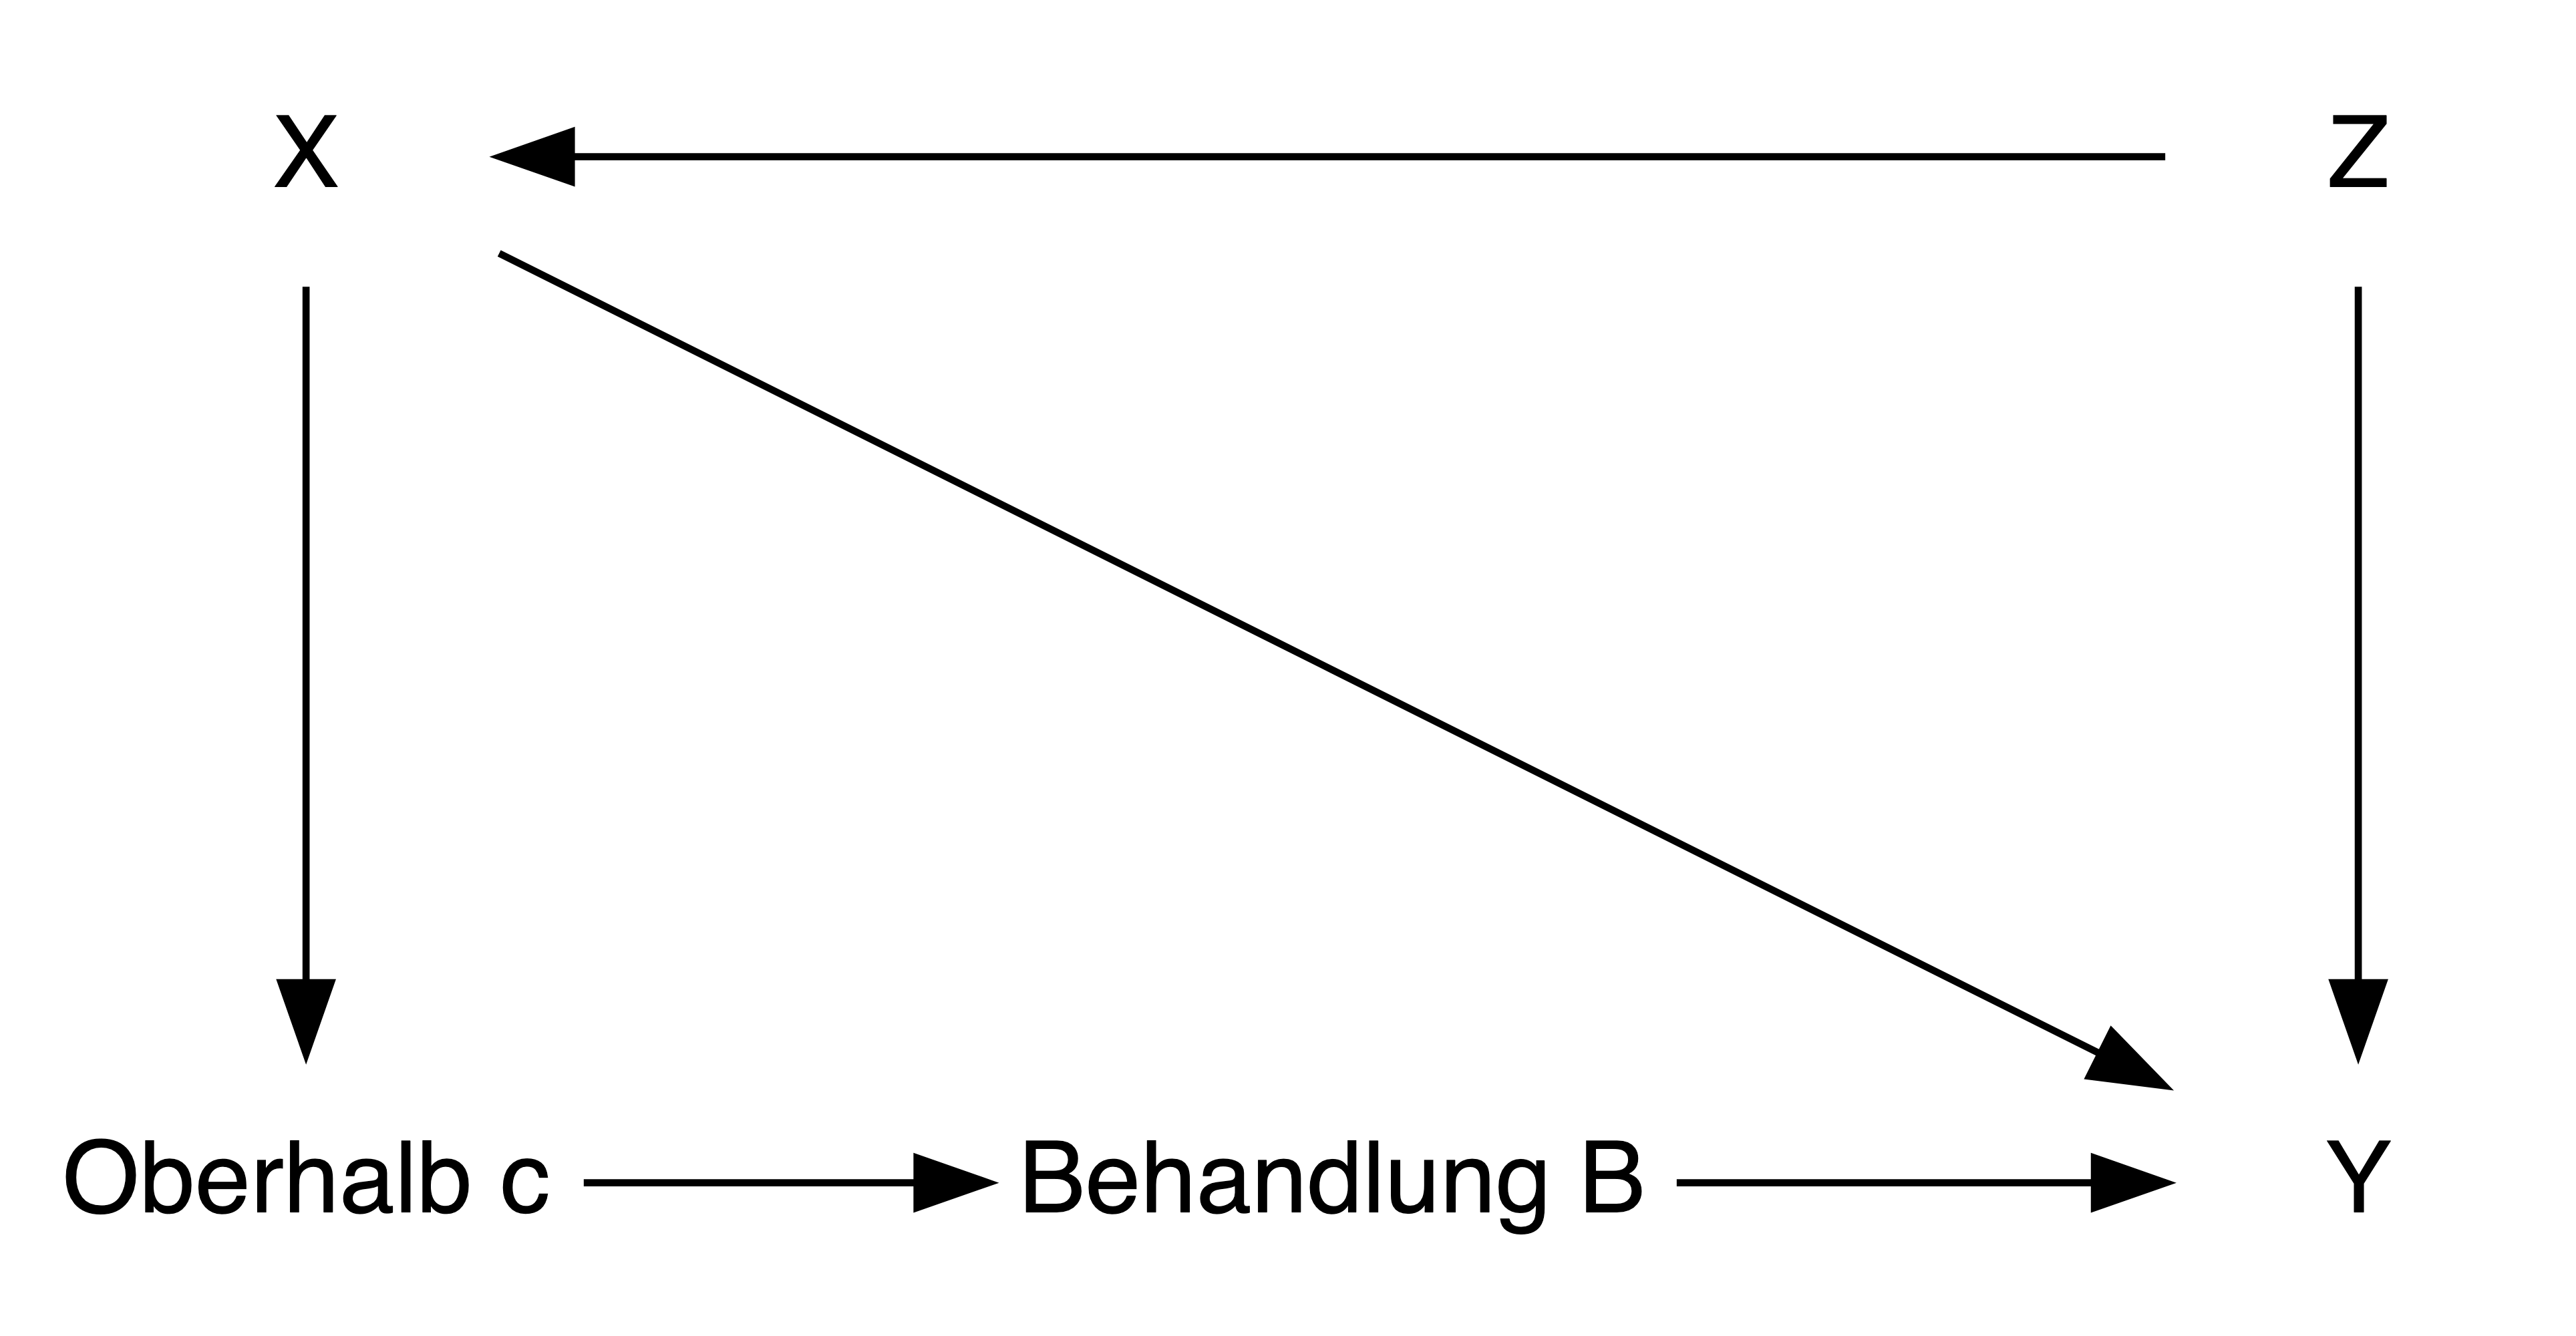
\includegraphics[width=5in,height=3in]{RDD_files/figure-latex/dot-figure-1.png}

}

\caption{\label{fig-CDRDD}Kausales Diagramm für Sharp RDD}

\end{figure}%

RDD isoliert Variation auf dem Pfad \emph{Oberhalb C → Behandlung B →
Y}. Somit können Backdoor-Pfade über \(X\) oder weitere (möglichweise
unbeobachtbare) Confounder (\(Z\)) vermieden werden, siehe
Abbildung~\ref{fig-CDRDD}. Der kausale Effekt wird dabei als (lokaler)
durchschnittlicher Behandlungseffekt der Diskontinuität auf die
Outcome-Variable (\(Y\)) anhand von Beobachtungen \emph{nahe bei c}
ermittelt.

Hinsichtlich der Beeinflussung der Behandlung unterscheiden wir zwischen
\emph{Sharp} und \emph{Fuzzy} Regression Discontinuity Designs
(SRDD/FRDD). Bei einem SRDD ist die Zuweisung der Behandlung
\emph{deterministisch}, d.h. der Schwellenwert in der Laufvariable ist
eine harte Grenze für die Gruppenzugehörigkeit: Die
\emph{Wahrscheinlichkeit} der Behandlung \(p\) springt bei \(X=c\) von
\(p=0\) um \(\Delta p = 1\) auf \(p=1\).

Bei einem FRDD ist die Zuordnung in Behandlungs- und Kontrollgruppe
nicht perfekt durch den Schwellenwert \(c\) bestimmt: Die
Behandlungswahrscheinlichkeit \(p\) springt bei \(X=c\) um
\(\Delta p<1\). Im FRDD können grundsätzlich also sowohl behandelte
Subjekte als auch Kontroll-Beobachtungen auf beiden Seiten der
Diskontinuität vorliegen -- die Trennung der Gruppen ist
``unscharf''\footnote{Engl. \emph{fuzzy}.}. Dieser Umstand ist oft in
empirischen Studien mit nicht-experimentellen Daten gegeben, wenn es
neben der Überschreitung von \(c\) weitere Determinanten der Behandlung
gibt (für die wir nicht kontrollieren können). Die Wahl zwischen SRDD
und FRDD hängt grundsätzlich vom datenerzeugenden Prozess und der
Forschungsfrage ab.

\section{Sharp Regression Discontinuity
Design}\label{sharp-regression-discontinuity-design}

\textbf{Modell und funktionale Form}

Die korrekte Spezifikation der funktionalen Form für ein RDD ist
wichtig, um eine verzerrte Schätzung des Effekts zu vermeiden. Die
einfachste Form eines SRDD kann anhand der linearen Regression
\begin{align}
Y_i = \beta_0 + \beta_1 B_i + \beta_2 X_i + u_i\label{eq-simpleSRDD}
\end{align} geschätzt werden, wobei \(B_i\) eine Dummy-Variable für das
Überschreiten des Schwellenwertes \(c\) ist, d.h. \begin{align*}
  B_i=\begin{cases}
    0 & X_i < c\\
    1 & X_i \geq c.
  \end{cases}
\end{align*} Damit ist \(B_i\) eine \emph{deterministische} Funktion der
Laufvariable \(X_i\) und zeigt die Zugehörigkeit zur Behandlungs- oder
Treatmentgruppe an. Der Koeffizient \(\beta_1\) misst den
Behandlungseffekt.

Das Modell \eqref{eq-simpleSRDD} unterstellt, dass \(X\) links- und
rechtsseitig von \(c\) denselben Effekt auf \(Y\) hat. Diese Annahme ist
restriktiv. Eine Alternative ist ein lineares Interaktionsmodell
\begin{align}
Y_i = \beta_0 + \beta_1 B_i + \beta_2 (X_i - c) + \beta_3(X_i - c)\times B_i + u_i.\label{eq:linearSRDD}
\end{align} Das Modell \eqref{eq:linearSRDD} kann unterschiedliche
lineare Effekte von \(X\) auf \(Y\) unterhalb (\(\beta_2\)) und oberhalb
(\(\beta_2 + \beta_3\)) von \(c\) abbilden. Beachte, dass \((X_i - c)\)
die um den Schwellenwert zentrierte Laufvariable ist, sodass \(\beta_1\)
wie in \eqref{eq-simpleSRDD} den Unterschied des Effekts von \(X\) auf
\(Y\) für Beoabachtungen am Schwellenwert erfasst.

Um unterschiedliche nicht-lineare Zusammenhänge von \(X\) und \(Y\)
unterhalb und oberhalb von \(c\) abzubilden, können (interargierte)
Polynom-Terme in \(X\) verwendet werden. Häufig wird eine quadratische
Regressionsfunktion genutzt, \begin{align}
  Y_i =&\, \beta_0 + \beta_1 B_i + \beta_2 (X_i - c) + \beta_3 (X_i - c)^2\\ 
       &+\, \beta_4(X_i - c)\times B_i + \beta_5(X_i - c)\times B_i + u_i.\label{eq:quadSRDD}
\end{align} Gelman und Imbens (2019) zeigen, dass Polynome höherer
Ordnung zu verzerrten Schätzern und hoher Varianz führen
können.\footnote{Ursachen sind Überanpassung an die Daten sowie
  instabiles Verhalten der Schätzung nahe des Schwellenwertes.} Die
Authoren empfehlen stattdessen die Schätzung mit lokaler Regression.

\textbf{Nicht-parametrische Schätzung und Bandweite}

Aktuelle Studien nutzen nicht-parametrische Schätzer, die den
Behandlungseffekt als Differenz der geschätzten Regressionsfunktionen am
Schwellenwert \(c\) berechnen. Um auch nicht-lineare
Regressionsfunktionen abzubilden zu können, wird häufig lokale
Regression verwendet. Dieses Verfahren liefert eine ``lokale'' Schätzung
der Regressionsfunktionen am Schwellenwert, bei der nur Beobachtungen
nahe \(X = c\) für die Schätzung berücksichtigt werden. Hinreichende
Nähe wird hierbei durch eine sogenannte Bandweite \(h\) festgelegt,
wobei \begin{align}
  \lvert(X_i-c)\rvert\leq h \label{eq:bwc}
\end{align} das Kriterium für eine Berücksichtigung von Beobachtung
\(i\) bei der Schätzung ist.

Unter Verwendung einer Bandweite \(h\) wird der Regressionsansatz
\eqref{eq:linearSRDD} als \emph{lokale lineare Regression} mit
Uniform-Kernelfunktion bezeichnet. Der Uniform-Kernel gibt allen
Beobachtungen, innerhalb der Bandweite \(h\) dasselbe Gewicht. Ist \(h\)
so groß, dass der gesamte Datensatz in die Schätzung einbezogen wird,
entspricht der lokale lineare Regressions-Schätzer mit Uniform-Kernel
dem (globalen) KQ-Schätzer in einem linearen Interaktionsmodell anhand
aller Beobachtungen. Neben dem Uniform-Kernel ist der Triangular-Kernel
eine in der Praxis häufig genutzte lineare Kernelfunktion. Der
nachstehende Code plottet die Uniform- (grün) sowie die
Triangular-Kernelfunktion (blau), siehe Abbildung~\ref{fig-linearkern}.

\begin{Shaded}
\begin{Highlighting}[]
\FunctionTok{library}\NormalTok{(ggplot2)}
\FunctionTok{library}\NormalTok{(cowplot)}

\CommentTok{\# Kernelfunktionen zeichnen}
\FunctionTok{ggplot}\NormalTok{() }\SpecialCharTok{+} 
    \FunctionTok{geom\_function}\NormalTok{(}
      \AttributeTok{fun =} \SpecialCharTok{\textasciitilde{}} \FunctionTok{ifelse}\NormalTok{(}
        \AttributeTok{test =} \FunctionTok{abs}\NormalTok{(.) }\SpecialCharTok{\textless{}=} \DecValTok{1}\NormalTok{,}
        \AttributeTok{yes =}  \DecValTok{1}\SpecialCharTok{/}\DecValTok{2}\NormalTok{, }
        \AttributeTok{no =} \DecValTok{0}
\NormalTok{      ), }
      \AttributeTok{col =} \StringTok{"green"}\NormalTok{, }
      \AttributeTok{n =} \DecValTok{1000}
\NormalTok{      ) }\SpecialCharTok{+} 
    \FunctionTok{geom\_function}\NormalTok{(}
      \AttributeTok{fun =} \SpecialCharTok{\textasciitilde{}} \FunctionTok{ifelse}\NormalTok{(}
        \AttributeTok{test =} \FunctionTok{abs}\NormalTok{(.) }\SpecialCharTok{\textless{}=} \DecValTok{1}\NormalTok{, }
        \AttributeTok{yes =} \DecValTok{1} \SpecialCharTok{{-}} \FunctionTok{abs}\NormalTok{(.), }
        \AttributeTok{no =} \DecValTok{0}
\NormalTok{      ), }
      \AttributeTok{col =} \StringTok{"blue"}\NormalTok{, }
      \AttributeTok{n =} \DecValTok{100}
\NormalTok{      ) }\SpecialCharTok{+} 
    \FunctionTok{scale\_x\_continuous}\NormalTok{(}
      \AttributeTok{name =} \StringTok{"x"}\NormalTok{, }
      \AttributeTok{limits =} \FunctionTok{c}\NormalTok{(}\SpecialCharTok{{-}}\FloatTok{1.5}\NormalTok{, }\FloatTok{1.5}\NormalTok{), }
      \AttributeTok{breaks =} \FunctionTok{c}\NormalTok{(}\SpecialCharTok{{-}}\DecValTok{1}\NormalTok{, }\DecValTok{0}\NormalTok{, }\DecValTok{1}\NormalTok{)}
\NormalTok{    ) }\SpecialCharTok{+}
    \FunctionTok{scale\_y\_continuous}\NormalTok{(}
      \AttributeTok{name =} \StringTok{"K(x)"}\NormalTok{, }
      \AttributeTok{breaks =} \FunctionTok{c}\NormalTok{(}\DecValTok{0}\NormalTok{, }\DecValTok{1}\NormalTok{), }
      \AttributeTok{limits =} \FunctionTok{c}\NormalTok{(}\DecValTok{0}\NormalTok{, }\FloatTok{1.25}\NormalTok{)}
\NormalTok{    ) }\SpecialCharTok{+}
    \FunctionTok{theme\_cowplot}\NormalTok{()}
\end{Highlighting}
\end{Shaded}

\begin{figure}[t]

\centering{

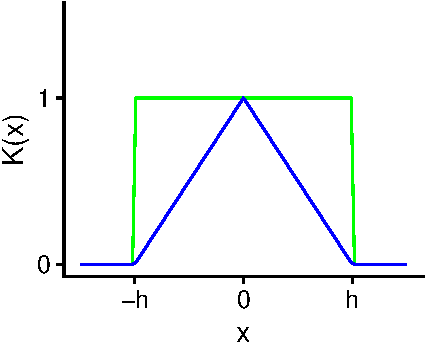
\includegraphics{RDD_files/figure-pdf/fig-linearkern-1.pdf}

}

\caption{\label{fig-linearkern}Kernelfunktionen auf {[}-1, 1{]}}

\end{figure}%

In empirischen Studien wird als Basis-Spezifikation oft eine lokale
lineare Regression anhand von \eqref{eq:linearSRDD} mit einer linearen
Kernelfunktionen und geringer bandweite \(h\) genutzt. Anschließend wird
die Robustheit der Ergebnisse anhand flexiblerer Spezifikationen, die
Nicht-Linearitäten in der Regressionsfunktion besser abbilden können,
geprüft.

Die nachstehende Visualisierung zeigt die Schätzung des kausalen
Effektes der Behandlung \(B_i\) anhand lokaler linearer Regression mit
einem Uniform-Kernel für wiefolgt simulierte Daten: \begin{align*}
  Y_i =&\, \beta_1 X_i + \beta_2 B + \beta_3 X_i^2 \times B_i + u_i,\\
  \\
  u_i \sim&\, N(0, 0.5), \quad X_i \sim U(0, 10), \quad B = \mathbb{I}(X_i \geq c = 5)\\
  \beta_1 =&\, .5, \quad \beta_2 = 1.5, \quad \beta_3 = -0.15
\end{align*}

Diese Vorschrift ist schnell mit R umgesetzt:

\begin{Shaded}
\begin{Highlighting}[]
\FunctionTok{set.seed}\NormalTok{(}\DecValTok{1234}\NormalTok{)}
\CommentTok{\# Anz.Beobachtungen}
\NormalTok{n }\OtherTok{\textless{}{-}} \DecValTok{750}

\CommentTok{\# Parameter definieren}
\NormalTok{c }\OtherTok{\textless{}{-}} \DecValTok{5}
\NormalTok{beta\_1 }\OtherTok{\textless{}{-}}\NormalTok{ .}\DecValTok{5}
\NormalTok{beta\_2 }\OtherTok{\textless{}{-}} \FloatTok{1.5}
\NormalTok{beta\_3 }\OtherTok{\textless{}{-}} \SpecialCharTok{{-}}\NormalTok{.}\DecValTok{15}

\CommentTok{\# Regressionsfunktion definieren}
\NormalTok{f }\OtherTok{\textless{}{-}} \ControlFlowTok{function}\NormalTok{(X) \{}
\NormalTok{  beta\_1 }\SpecialCharTok{*}\NormalTok{ (X }\SpecialCharTok{{-}}\NormalTok{ c) }\SpecialCharTok{+}\NormalTok{ beta\_2 }\SpecialCharTok{*}\NormalTok{ B }\SpecialCharTok{+}\NormalTok{ beta\_3 }\SpecialCharTok{*}\NormalTok{ B }\SpecialCharTok{*}\NormalTok{ (X }\SpecialCharTok{{-}}\NormalTok{ c)}\SpecialCharTok{\^{}}\DecValTok{2}
\NormalTok{\}}

\CommentTok{\# Daten erzeugen}
\NormalTok{X }\OtherTok{\textless{}{-}} \FunctionTok{runif}\NormalTok{(n, }\DecValTok{0}\NormalTok{, }\DecValTok{11}\NormalTok{)}
\NormalTok{B }\OtherTok{\textless{}{-}} \FunctionTok{ifelse}\NormalTok{(X }\SpecialCharTok{{-}}\NormalTok{ c }\SpecialCharTok{\textgreater{}=} \DecValTok{0}\NormalTok{, }\DecValTok{1}\NormalTok{, }\DecValTok{0}\NormalTok{)}
\NormalTok{Y }\OtherTok{\textless{}{-}} \FunctionTok{f}\NormalTok{(X) }\SpecialCharTok{+} \FunctionTok{rnorm}\NormalTok{(n, }\AttributeTok{sd =}\NormalTok{ .}\DecValTok{5}\NormalTok{)}

\CommentTok{\# Beoabchtungen sammeln}
\NormalTok{dat }\OtherTok{\textless{}{-}} \FunctionTok{data.frame}\NormalTok{(}
  \AttributeTok{Y =}\NormalTok{ Y, }\AttributeTok{X =}\NormalTok{ X }\SpecialCharTok{{-}}\NormalTok{ c, }\AttributeTok{B =}\NormalTok{ B}
\NormalTok{)}
\end{Highlighting}
\end{Shaded}

\begin{center}\rule{0.5\linewidth}{0.5pt}\end{center}

\textbf{\emph{Diese interaktive Komponente des Buchs ist nur in der
Online-Version verfügbar.}}

\begin{center}\rule{0.5\linewidth}{0.5pt}\end{center}

Der interssierende Effekt am Schwellenwert \(c=5\) beträgt
\(\beta_2 = 1.5\). Beachte, dass aufgrund des Terms
\(\beta_3 X_i^2 \times B_i\) ein quadratischer Zusammenhang von \(Y\)
und \(X\) oberhalb von \(X_i = c\) vorliegt. Es können folgende
Eigenschaften der Schätzung in Abhängigkeit von der Bandweite \(h\)
beobachtet werden:

\begin{itemize}
\item
  Für die voreingestellte Bandweite \(h = 1.3\) liefert die lokale
  lineare Regression eine gute Approximation des
  Regressionszusammenhangs auf beiden Seiten des Schwellenwertes und die
  Schätzung des Behandlungseffekts liegt nahe beim wahren Wert
  \(\beta_2 = 1.5\).
\item
  Für kleinere Bandweiten verringert sich die Datenbasis der Schätzung.
  Die Varianz der Schätzung nimmt zu und die Approximation der
  Regressionsfunktion verschlechtert sich. Wir beobachten eine mit
  \(h\to0\) zunehmende Verzerrung bei der Schätzung des
  Behandlungseffekts.
\item
  Größere Bandweiten \(h\) erhöhen die Datenbasis der Schätzung, führen
  aber zu einer Annäherung der lokalen Schätzung an die globale
  KQ-Schätzung. Linksseitig des Schwellenwertes erzielen wir damit eine
  Schätzung mit hoher Güte. Rechsseitig von \(X_i = c\) verschlechtert
  sich die lokale Anpassung am Schwellenwert deutlich, weil die lineare
  Schätzung den tatsächlichen (nicht-linearen) Zusammenhang nicht
  adäquat abbilden kann. Die Schätzung des Behandlungseffekts ist hier
  deutlich verzerrt.
\end{itemize}

Die Wahl der Bandweite ist also eine wichtige Komponenten der
RDD-Schätzung: Kleine Bandweiten erlauben eine Schätzung der
Regressionsfunktion nahe des Schwellenwertes mit wenig Verzerrung.
Allerdings kann diese Schätzung unpräzise sein, wenn nur wenige
Beobachtungen \eqref{eq:bwc} erfüllen. In der Praxis wird \(h\) daher
mit einem analytischen Schätzer (vgl. G. Imbens und Kalyanaraman 2012)
oder anhand von \emph{Cross Validation} (bspw. G. W. Imbens und Lemieux
2008) bestimmt. Die später in diesem Kapitel betrachteten R-Pakete
halten diese Methoden bereit.

\section{Manipulation am
Schwellenwert}\label{manipulation-am-schwellenwert}

Eine wichtige Annahmen für die Gültigkeit einer RDD-Schätzung ist, dass
keine Manipulation der Gruppenzugehörigkeit am Schwellenwert vorliegt.
Wenn sich Subjekte nahe des Schwellenwertes \(c\) --- d.h. in
Abhängigkeit der Laufvariable \(X\) --- systematisch in den Confoundern
\(Z\) unterscheiden, können wir den Backdoor-Pfad \emph{Oberhalb C →
Behandlung B → Y} nicht isolieren. Wir erhalten dann eine verzerrte
Schätzung des Behandlungseffekts.

In empirischen Studien mit Individuen kann Selbstselektion auftreten:
Menschen mit \(X<c\) aber nahe \(c\) (hier Kontrollgruppe) könnten
aufgrund unbeobachtbarer Eigenschaften \(Z\) die Ausprägung ihrer
Laufvariable zu \(X>c\) (hier Behandlungsgruppe) manipulieren. Wenn
\(Z\) die Outcome-Variable beeinflusst, bleibt der Backdoor-Pfad
\emph{Oberhalb C → Behandlung B → Y} so bestehen.

Manipulation resultiert in Häufung von Beobachtungen am Schwellenwert.
Dei Verteilung der Laufvariable kann auf diese Unregelmäßigkeit hin
untersucht werden. McCrary (2008) schlägt hierfür einen Verfahren vor,
das die Kontinuität der Dichtefunktion von \(X\) am Schwellenwert
testet.

Der Test von McCrary (2008) ist in \texttt{rdd::DCdensity()}
implementiert. Wir zeigen die Anwendung des Tests anhand der oben
simulierten Daten. Beachte, dass \(X_i\sim U(0, 10)\), d.h. die
Laufvariable ist bei \(X_i = c\) kontinuierlich verteilt. Die
Nullhypothese (keine Manipulation) gilt für die simulierten Daten

\begin{Shaded}
\begin{Highlighting}[]
\CommentTok{\# McCrary{-}Test durchführen}
\NormalTok{p\_mccrary }\OtherTok{\textless{}{-}}\NormalTok{ rdd}\SpecialCharTok{::}\FunctionTok{DCdensity}\NormalTok{(}
  \AttributeTok{runvar =}\NormalTok{ X, }
  \AttributeTok{cutpoint =}\NormalTok{ c, }
  \AttributeTok{plot =}\NormalTok{ F}
\NormalTok{)}

\CommentTok{\# p{-}Wert}
\NormalTok{p\_mccrary}
\end{Highlighting}
\end{Shaded}

\begin{verbatim}
[1] 0.5013939
\end{verbatim}

Der p-Wert 0.5 ist größer als jedes übliche Signifikanzniveau. Damit
liegt starke Evidenz für die Nullhypothese (keine Diskontinuität) und
gegen Manipulation am Schwellenwert vor.

Cattaneo, Jansson, und Ma (2020) (CMJ) schlagen eine Weiterentwicklung
des McCrary-Tests vor, die höhere statistische Macht gegenüber
Diskontinuitäten hat am Schwellenwert hat. Der CJM-Test ist im Paket
\texttt{rddensity} implementiert.

\begin{Shaded}
\begin{Highlighting}[]
\FunctionTok{library}\NormalTok{(rddensity)}

\CommentTok{\# CJM Schätzer berechnen}
\NormalTok{CJM }\OtherTok{\textless{}{-}} \FunctionTok{rddensity}\NormalTok{(X, }\AttributeTok{c =} \DecValTok{5}\NormalTok{)}
\end{Highlighting}
\end{Shaded}

Mit der Funktion \texttt{rddensity::rdplotdensity()} erzeugen wir
Abbildung~\ref{fig-cjmtsim}.

\begin{Shaded}
\begin{Highlighting}[]
\CommentTok{\# Plot für Dichtefunktion erstellen}
\NormalTok{plot }\OtherTok{\textless{}{-}} \FunctionTok{rdplotdensity}\NormalTok{(}
  \AttributeTok{rdd =}\NormalTok{ CJM, }
  \AttributeTok{X =}\NormalTok{ X, }
  \CommentTok{\# für Punkte{-} und Linienplots:}
  \AttributeTok{type =} \StringTok{"both"} 
\NormalTok{)}
\end{Highlighting}
\end{Shaded}

\begin{figure}[t]

\centering{

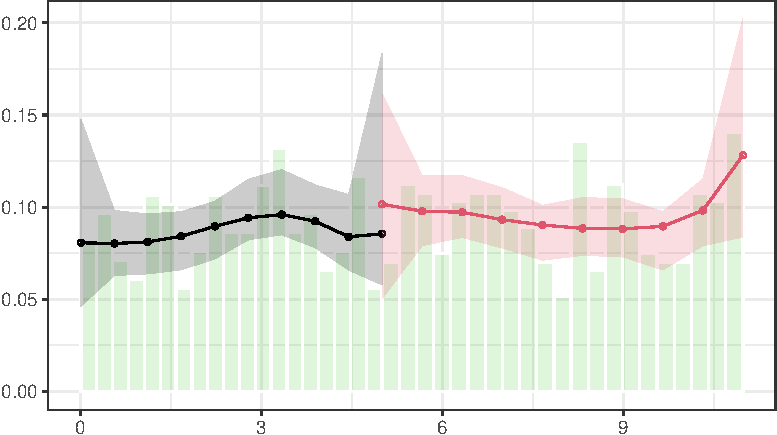
\includegraphics{RDD_files/figure-pdf/fig-cjmtsim-1.pdf}

}

\caption{\label{fig-cjmtsim}CJM-Test -- geschätzte Dichtefunktionen der
Laufvariable auf beiden Seiten des Schwellenwerts c = 5}

\end{figure}%

Abbildung~\ref{fig-cjmtsim} zeigt die geschätzten Dichtefunktionen.
Erwartungsgemäß finden wir eine große Überlappung der zugehörigen
Konfidenzbänder (schattierte Flächen) am Schwellenwert \(c=5\).

Mit \texttt{summary()} erhalten wir eine detaillierte Zusammenfassung
des Tests.

\begin{Shaded}
\begin{Highlighting}[]
\CommentTok{\# Statistische Zusammenfassung des CJM{-}Tests}
\FunctionTok{summary}\NormalTok{(CJM)}
\end{Highlighting}
\end{Shaded}

\begin{verbatim}

Manipulation testing using local polynomial density estimation.

Number of obs =       750
Model =               unrestricted
Kernel =              triangular
BW method =           estimated
VCE method =          jackknife

c = 5                 Left of c           Right of c          
Number of obs         329                 421                 
Eff. Number of obs    133                 154                 
Order est. (p)        2                   2                   
Order bias (q)        3                   3                   
BW est. (h)           1.918               2.124               

Method                T                   P > |T|             
Robust                -0.3338             0.7385              


P-values of binomial tests (H0: p=0.5).

Window Length              <c     >=c    P>|T|
0.346     + 0.346          20      21    1.0000
0.521     + 0.544          34      37    0.8126
0.696     + 0.742          44      57    0.2323
0.870     + 0.939          54      64    0.4075
1.045     + 1.137          62      77    0.2349
1.220     + 1.334          73      98    0.0661
1.394     + 1.532          86     106    0.1701
1.569     + 1.729          96     124    0.0685
1.743     + 1.927         119     140    0.2139
1.918     + 2.124         133     154    0.2377
\end{verbatim}

Gemäß des p-Werts (\texttt{P\ \textgreater{}\ \textbar{}T\textbar{}})
von 0.74 spricht der CJM-Test noch deutlicher gegen eine Diskontinuität
als der McCrary-Test.

\subsection{Case Study: Amtsinhaber-Vorteil (Lee
2008)}\label{case-study-amtsinhaber-vorteil-lee2008}

Lee (2008) untersucht den Einfluss des Amtsinhaber-Vorteils auf die Wahl
von Mitgliedern des US-Repräsentantenhaus. In den meisten Wahlkreisen
entfallen große Anteile der Stimmen (oder gar ausschließlich) auf
demokratische und republikanische Kanditat*innen, sodass sich die Studie
auf diese Parteien beschränkt. Entfällt die Mehrheit der Stimmen auf
eine*n Kandiat*in, gewinnt diese*r den Sitz für den Wahlkreis. Durch die
Analyse der 6558 Wahlen im Zeitraum 1946-1998 mit einem SRDD kommt die
Studie zu dem Ergebnis, dass Amtsinhabende im Durchschnitt einen Vorteil
von etwa 8\% bis 10\% bei der Wahl haben. Dieses Ergebnis kann
verschiedene Ursachen haben, bspw. dass die amtierende Partei höhere
finanzielle Ressourcen besitzt und von einer besseren Organisation und
durch Instrumenalisierung staatlicher Strukturen für die eigenen Zwecke
profitiert.

Anhand der Datensätze \texttt{house} und \texttt{house\_binned}
illustrieren wir nachfolgend die Schätzung von SRDD-Modellen für den
Wahlerfolg der demokratischen Partei, wenn diese Amtsinhaber ist. Wir
lesen hierfür zunächst die Datensätze \texttt{house} und
\texttt{house\_binned} ein und verschaffen uns einen Überblick.

\begin{Shaded}
\begin{Highlighting}[]
\FunctionTok{library}\NormalTok{(tidyverse)}
\FunctionTok{library}\NormalTok{(modelsummary)}

\CommentTok{\# Daten einlesen}
\NormalTok{house }\OtherTok{\textless{}{-}} \FunctionTok{read\_csv}\NormalTok{(}\StringTok{"datasets/house.csv"}\NormalTok{)}
\CommentTok{\# Gruppierter Datensatz}
\NormalTok{house\_binned }\OtherTok{\textless{}{-}} \FunctionTok{read\_csv}\NormalTok{(}\StringTok{"datasets/house\_binned.csv"}\NormalTok{)}

\CommentTok{\# Überblick verschaffen}
\FunctionTok{glimpse}\NormalTok{(house)}
\end{Highlighting}
\end{Shaded}

\begin{verbatim}
Rows: 6,558
Columns: 2
$ StimmenTm1 <dbl> 0.1049, 0.1393, -0.0736, 0.0868, 0.3994, 0.1681, 0.2516, 0.~
$ StimmenT   <dbl> 0.5810, 0.4611, 0.5434, 0.5846, 0.5803, 0.6244, 0.4873, 0.5~
\end{verbatim}

\begin{Shaded}
\begin{Highlighting}[]
\FunctionTok{glimpse}\NormalTok{(house\_binned)}
\end{Highlighting}
\end{Shaded}

\begin{verbatim}
Rows: 100
Columns: 2
$ StimmenT   <dbl> 0.5995600, 0.5657000, 0.4272554, 0.5637456, 0.6868627, 0.60~
$ StimmenTm1 <dbl> 0.104764444, 0.135005263, -0.075690769, 0.084570886, 0.3951~
\end{verbatim}

Der Datensatz \texttt{house} enthält die Stimmenanteile demokratischer
Kandidat*innen bei der Wahl zum Zeitpunkt \(T\) (\(StimmenT\)) sowie die
Differenz zwischen demokratischen und republikanischen Stimmenanteilen
bei der vorherigen Wahl, d.h. zum Zeitpunkt \(T-1\) (\(StimmenTm1\)).
Der Schwellenwert für einen Wahlsieg liegt bei Stimmengleichheit, d.h.
\(StimmenTm1 = 0\).

\texttt{house\_binned} ist eine aggregierte Version von \texttt{house}
mit Mittelwerten von jeweils 50 gleichgroßen Intervallen oberhalb und
unterhalb der Schwelle von \(StimmenTm1 = 0\). Dieser Datensatz eignet
sich, um einen ersten Eindruck des funktionalen Zusammenhangs auf beiden
Seiten zu erhalten. Wir stellen zunächst diese klassierten Daten mit
\texttt{ggplot2} graphisch dar.

\begin{Shaded}
\begin{Highlighting}[]
\CommentTok{\# Klassierte Daten plotten}
\NormalTok{house\_binned }\SpecialCharTok{\%\textgreater{}\%}
  \FunctionTok{ggplot}\NormalTok{(}
    \FunctionTok{aes}\NormalTok{(}\AttributeTok{x =}\NormalTok{ StimmenTm1, }\AttributeTok{y =}\NormalTok{ StimmenT)}
\NormalTok{    ) }\SpecialCharTok{+}
  \FunctionTok{geom\_point}\NormalTok{() }\SpecialCharTok{+}
  \FunctionTok{geom\_vline}\NormalTok{(}\AttributeTok{xintercept =} \DecValTok{0}\NormalTok{, }\AttributeTok{lty =} \DecValTok{2}\NormalTok{)}
\end{Highlighting}
\end{Shaded}

\begin{figure}[t]

\centering{

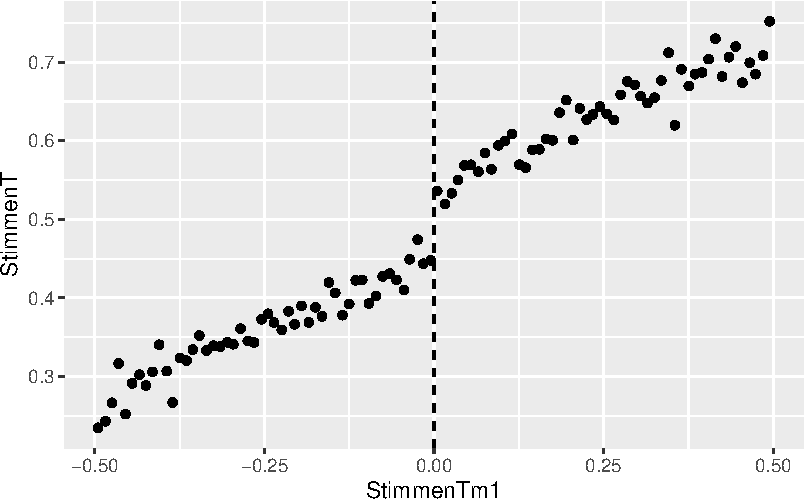
\includegraphics{RDD_files/figure-pdf/fig-LeeDataClass-1.pdf}

}

\caption{\label{fig-LeeDataClass}Klassierte Daten aus Lee (2008)}

\end{figure}%

Die Grafik zeigt eindeutig einen Sprung von \(StimmenT\) bei
\(StimmenTm1 = 0\). Weiterhin erkennen wir, dass der Zusammenhang nahe
\(0\) vermutlich jeweils gut durch eine lineare Funktion approximiert
werden kann. Eine Modell-Spezifikation mit gleicher Steigung auf beiden
Seiten des Schwellenwertes scheint hingegen weniger gut geeignet. Wir
vergleichen diese Spezifikationen nachfolgend.

Zunächst fügen wir dem Datensatz eine Dummyvariable \texttt{B} hinzu.
Diese dient als Indikator für den Wahlgewinn in der letzten Wahl und
zeigt die Amtsinhaberschaft (Behandlung) an.

\begin{Shaded}
\begin{Highlighting}[]
\CommentTok{\# Behandlungsindikator B hinzufügen}
\NormalTok{house }\OtherTok{\textless{}{-}}\NormalTok{ house }\SpecialCharTok{\%\textgreater{}\%} 
  \FunctionTok{mutate}\NormalTok{(}\AttributeTok{B =}\NormalTok{ StimmenTm1 }\SpecialCharTok{\textgreater{}} \DecValTok{0}\NormalTok{)}

\FunctionTok{glimpse}\NormalTok{(house)}
\end{Highlighting}
\end{Shaded}

\begin{verbatim}
Rows: 6,558
Columns: 3
$ StimmenTm1 <dbl> 0.1049, 0.1393, -0.0736, 0.0868, 0.3994, 0.1681, 0.2516, 0.~
$ StimmenT   <dbl> 0.5810, 0.4611, 0.5434, 0.5846, 0.5803, 0.6244, 0.4873, 0.5~
$ B          <lgl> TRUE, TRUE, FALSE, TRUE, TRUE, TRUE, TRUE, TRUE, TRUE, TRUE~
\end{verbatim}

Wir überprüfen die Laufvariable mit dem CJM-Test auf Manipulation am
Schwellenwert \(c=0\).

\begin{Shaded}
\begin{Highlighting}[]
\CommentTok{\# CJM{-}Test durchführen}
\NormalTok{CJM\_Lee }\OtherTok{\textless{}{-}} \FunctionTok{rddensity}\NormalTok{(}\AttributeTok{X =}\NormalTok{ house}\SpecialCharTok{$}\NormalTok{StimmenTm1)}

\CommentTok{\# Zusammenfassung anzeigen}
\FunctionTok{summary}\NormalTok{(CJM\_Lee)}
\end{Highlighting}
\end{Shaded}

\begin{verbatim}

Manipulation testing using local polynomial density estimation.

Number of obs =       6558
Model =               unrestricted
Kernel =              triangular
BW method =           estimated
VCE method =          jackknife

c = 0                 Left of c           Right of c          
Number of obs         2740                3818                
Eff. Number of obs    1297                1360                
Order est. (p)        2                   2                   
Order bias (q)        3                   3                   
BW est. (h)           0.236               0.243               

Method                T                   P > |T|             
Robust                1.4346              0.1514              


P-values of binomial tests (H0: p=0.5).

Window Length / 2          <c     >=c    P>|T|
0.004                      21      24    0.7660
0.007                      38      46    0.4452
0.011                      50      60    0.3909
0.014                      73      77    0.8066
0.018                      91     104    0.3902
0.022                     124     132    0.6618
0.025                     149     149    1.0000
0.029                     163     174    0.5860
0.032                     176     202    0.1984
0.036                     197     223    0.2225
\end{verbatim}

\begin{Shaded}
\begin{Highlighting}[]
\CommentTok{\# CJM{-}Plot}
\NormalTok{plot }\OtherTok{\textless{}{-}} \FunctionTok{rdplotdensity}\NormalTok{(}
  \AttributeTok{rdd =}\NormalTok{ CJM\_Lee,}
  \AttributeTok{X =}\NormalTok{ house}\SpecialCharTok{$}\NormalTok{StimmenTm1, }
  \AttributeTok{type =} \StringTok{"both"}\NormalTok{, }
\NormalTok{)}
\end{Highlighting}
\end{Shaded}

\begin{figure}[t]

\centering{

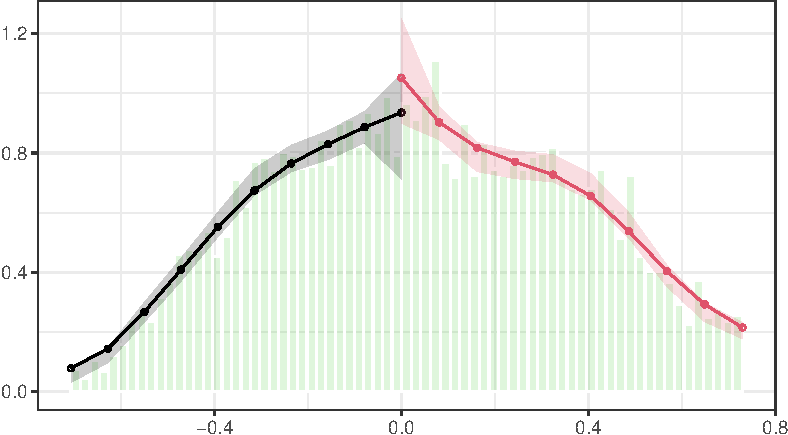
\includegraphics{RDD_files/figure-pdf/fig-cjm-lee-1.pdf}

}

\caption{\label{fig-cjm-lee}CJM-Test -- geschätzte Dichtefunktionen der
Laufvariable}

\end{figure}%

Abbildung~\ref{fig-cjm-lee} und der p-Wert von \(0.15\) sind Evidenz
gegen eine Manipulation am Schwellenwert.

Um den Behandlungseffekt anhand eines SRDDs zu ermitteln, schätzen wir
das Interaktionsmodell \begin{align*}
  \text{StimmenT}_i =&\, \beta_0 + \beta_1 B_i + \beta_2 (\text{StimmenTm1}_i - 50)\\ 
  +&\, \beta_3(\text{StimmenTm1}_i - 50)\times B_i + u_i
\end{align*} zunächst für eine Bandweite von \(h = 0.5\). Aufgrund der
Skalierung der Daten (Wahlergebnisse in \%) bedeutet dies die Verwendung
des \emph{gesamten} Datensatzes für die Schätzung.

\begin{Shaded}
\begin{Highlighting}[]
\CommentTok{\# Interaktionsmodell schätzen}
\NormalTok{house\_llr1 }\OtherTok{\textless{}{-}} \FunctionTok{lm}\NormalTok{(}
  \AttributeTok{formula =}\NormalTok{ StimmenT }\SpecialCharTok{\textasciitilde{}}\NormalTok{ B }\SpecialCharTok{*}\NormalTok{ StimmenTm1, }
  \AttributeTok{data =}\NormalTok{ house}
\NormalTok{)}

\CommentTok{\# Zusammenfassung anzeigen  }
\FunctionTok{modelsummary}\NormalTok{(}
  \AttributeTok{models =}\NormalTok{ house\_llr1, }
  \AttributeTok{vcov =} \StringTok{"HC1"}\NormalTok{, }\CommentTok{\# robuste Standardfehler}
  \AttributeTok{stars =}\NormalTok{ T, }
  \AttributeTok{gof\_map =} \StringTok{"nobs"}\NormalTok{, }
  \AttributeTok{output =} \StringTok{"gt"}
\NormalTok{) }\SpecialCharTok{\%\textgreater{}\%} 
\NormalTok{  tabopts}
\end{Highlighting}
\end{Shaded}

\setlength{\LTpost}{0mm}
\begin{longtable*}{lc}
\toprule
  & (1) \\ 
\midrule\addlinespace[2.5pt]
(Intercept) & 0.433*** \\ 
 & (0.004) \\ 
BTRUE & 0.118*** \\ 
 & (0.006) \\ 
StimmenTm1 & 0.297*** \\ 
 & (0.016) \\ 
BTRUE × StimmenTm1 & 0.046* \\ 
 & (0.018) \\ 
Num.Obs. & 6558 \\ 
\bottomrule
\end{longtable*}
\begin{minipage}{\linewidth}
+ p < 0.1, * p < 0.05, ** p < 0.01, *** p < 0.001\\
\end{minipage}

Der geschätzte Koeffizient von \(B\) (\texttt{BTRUE}) beträgt etwa
\(0.12\) und ist hochsignifikant. Übereinstimmend mit
Abbildung~\ref{fig-LeeDataClass} erhalten wir also eine positive
Schätzung des Behandlungseffekts. Die Interpretation ist, dass die
amtierenden Demokraten bei der Wahl von einem Amtsinhabervorteil
profitieren. Dieser Effekt schlägt sich als Stimmenbonus von geschätzten
12\% nieder. Diese Schätzung des Behandlungseffekts könnte jedoch
verzerrt sein:

\begin{itemize}
\item
  Die (implizite) Wahl von \(h=0.5\) in unserer Schätzung macht die
  Isolation des relevanten Frontdoor-Paths (\(c=0\) → Treatment →
  StimmenT) wenig plausibel. \(h\) sollte mit einer datengetriebenen
  Methode gewählt werden.
\item
  Weiterhin könnte die lineare funktionale Form der Regression inadäquat
  sein: Die lineare Approximation der wahren Regressionsfunktion nahe
  des Schwellenwerts \(0\) könnte unzureichend sein und in einer
  verzerrten Schätzung des Effekts resultieren. Zur Überprüfung der
  Robustheit der Ergebnisse sollte mit Schätzungen anhand nicht-linearer
  Spezifikationen verglichen werden.
\end{itemize}

Um diesen Gefahren für die Validität der Studie zu begegnen, schätzen
wir nun weitere Spezifikationen. Im Folgenden verwenden wir eine
Bandweitenschätzung gemäß G. Imbens und Kalyanaraman (2012).

\begin{Shaded}
\begin{Highlighting}[]
\CommentTok{\# Bandweite mit Schätzer von IK (2012) berechnen}
\NormalTok{(}
\NormalTok{IK\_BW }\OtherTok{\textless{}{-}} 
\NormalTok{  rdd}\SpecialCharTok{::}\FunctionTok{IKbandwidth}\NormalTok{(}
    \AttributeTok{X =}\NormalTok{ house}\SpecialCharTok{$}\NormalTok{StimmenTm1, }
    \AttributeTok{Y =}\NormalTok{ house}\SpecialCharTok{$}\NormalTok{StimmenT}
\NormalTok{  )}
\NormalTok{)}
\end{Highlighting}
\end{Shaded}

\begin{verbatim}
[1] 0.2685123
\end{verbatim}

Wir schätzen zunächst erneut das lineare Interaktionsmodell, diesmal
jedoch mit der Bandweite \texttt{IK\_BW}.

\begin{Shaded}
\begin{Highlighting}[]
\CommentTok{\# Lineares Interaktionsmodelle mit IK{-}Bandweite}
\NormalTok{house\_llin\_IK }\OtherTok{\textless{}{-}} \FunctionTok{lm}\NormalTok{(}
  \AttributeTok{formula =}\NormalTok{ StimmenT }\SpecialCharTok{\textasciitilde{}}\NormalTok{ B }\SpecialCharTok{*}\NormalTok{ StimmenTm1, }
  \AttributeTok{data =}\NormalTok{ house }\SpecialCharTok{\%\textgreater{}\%} 
    \FunctionTok{filter}\NormalTok{(}
      \FunctionTok{abs}\NormalTok{(StimmenTm1) }\SpecialCharTok{\textless{}=}\NormalTok{ IK\_BW}
\NormalTok{    )}
\NormalTok{)}
\end{Highlighting}
\end{Shaded}

Für den Vergleich mit einer nicht-linearen Spezifikation schätzen wir
auch ein quadratisches Interaktionsmodell.

\begin{Shaded}
\begin{Highlighting}[]
\CommentTok{\# Quadratisches Interaktionsmodell mit IK{-}Bandweite}
\NormalTok{house\_poly\_IK }\OtherTok{\textless{}{-}} \FunctionTok{update}\NormalTok{(}
  \AttributeTok{object =}\NormalTok{ house\_llin\_IK,}
  \AttributeTok{formula =}\NormalTok{ StimmenT }\SpecialCharTok{\textasciitilde{}}\NormalTok{ B }\SpecialCharTok{*} \FunctionTok{poly}\NormalTok{(StimmenTm1, }\AttributeTok{degree =} \DecValTok{2}\NormalTok{, }\AttributeTok{raw =}\NormalTok{ T)}
\NormalTok{)}
\end{Highlighting}
\end{Shaded}

Für eine Gegenüberstellung der Ergebnisse verwenden wir
\texttt{modelsummary()}.

\begin{Shaded}
\begin{Highlighting}[]
\CommentTok{\# Tabellarischer Modellvergleich}
\FunctionTok{modelsummary}\NormalTok{(}
  \AttributeTok{models =} \FunctionTok{list}\NormalTok{(}
    \StringTok{"Linear int."} \OtherTok{=}\NormalTok{ house\_llin\_IK, }
    \StringTok{"Quadratisch int."} \OtherTok{=}\NormalTok{ house\_poly\_IK}
\NormalTok{  ),  }
  \AttributeTok{vcov =} \StringTok{"HC1"}\NormalTok{, }
  \AttributeTok{stars =}\NormalTok{ T,}
  \AttributeTok{gof\_map =} \StringTok{"nobs"}\NormalTok{, }
  \AttributeTok{output =} \StringTok{"gt"}
\NormalTok{) }\SpecialCharTok{\%\textgreater{}\%} 
\NormalTok{  tabopts}
\end{Highlighting}
\end{Shaded}

\setlength{\LTpost}{0mm}

\begin{longtable}{lcc}

\caption{\label{tbl-intmodsLee}Vergleich von SRDD-Interaktionsmodellen
für Lee (2008)}

\tabularnewline

\toprule
  & Linear int. & Quadratisch int. \\ 
\midrule\addlinespace[2.5pt]
(Intercept) & 0.450*** & 0.460*** \\ 
 & (0.005) & (0.008) \\ 
BTRUE & 0.085*** & 0.068*** \\ 
 & (0.008) & (0.012) \\ 
StimmenTm1 & 0.360*** &  \\ 
 & (0.036) &  \\ 
BTRUE × StimmenTm1 & 0.055 &  \\ 
 & (0.059) &  \\ 
poly(StimmenTm1, degree = 2, raw = T)1 &  & 0.573*** \\ 
 &  & (0.138) \\ 
poly(StimmenTm1, degree = 2, raw = T)2 &  & 0.798 \\ 
 &  & (0.493) \\ 
BTRUE × poly(StimmenTm1, degree = 2, raw = T)1 &  & 0.036 \\ 
 &  & (0.219) \\ 
BTRUE × poly(StimmenTm1, degree = 2, raw = T)2 &  & -1.529+ \\ 
 &  & (0.834) \\ 
Num.Obs. & 2956 & 2956 \\ 
\bottomrule

\end{longtable}

\begin{minipage}{\linewidth}
+ p < 0.1, * p < 0.05, ** p < 0.01, *** p < 0.001\\
\end{minipage}

Die Spalte (1) in Tabelle~\ref{tbl-intmodsLee} zeigt die lokale
Schätzung mit einem linearen Interaktionsmodell. Wir erhalten damit
einen Behandlungseffekt von etwa \(8.5\%\). Der Schätzwert fällt also
etwas geringer aus als für die globale KQ-Schätzung des linearen
Interaktionsmodells. Für das Modell (2) mit quadratischer Spezifikation
liegt der Schätzwert mit \(6.8\%\) in der selben Größenordnung. Beide
Schätzungen ergeben einen signifikant von \(0\) verschieden Effekt.
Weiterhin fällt auf, dass in beiden Modellen keine Evidenz für
unterschiedliche Formen der Regressionsfunktionen auf beiden Seiten des
Schwellenwerts vorliegen: sämtliche Koeffizientenschätzwerte der
Interaktionsterme haben hohe Standardfehler und sind nicht signifikant.
Im quadratischen Modell hat auch der Term \(StimmenTm1^2\) keinen
signifikanten Effekt. Diese Ergebnisse deuten darauf hin, dass eine
lineare Spezifikation ausreichend ist.

\textbf{SRDD-Schätzung mit LOESS}

Wir illustrieren nachfolgend die Schätzung des Behandlungseffekts mit
einer flexiblen und in der Praxis häufig verwendeten Methode für lokale
Regression. Die nachfolgende interaktive Grafik zeigt die klassierten
Daten aus Lee (2008) auf dem Intervall \([-0.5,0.5]\) gemeinsam mit
einer nicht-parametrischen Schätzung des Zusammenhangs von
\texttt{StimmenT} und \texttt{StimmenTm1} mittels LOESS.\footnote{\href{https://en.wikipedia.org/wiki/Local_regression}{LOESS}
  ist eine Variante von lokaler Polynom-Regression.} Diese
Implementierung von lokaler Regression nutzt einen
\href{https://en.wikipedia.org/wiki/Kernel_(statistics)}{tricube
kernel}. Über den Input kann eine Bandweite \(l\in(0,1]\) für den
LOESS-Schätzer auf beiden Seiten des Schwellenwerts \(0\) gewählt
werden. Die Bandweite ist hier der \emph{Anteil der Beobachtungen an der
gesamten Anzahl an Beobachtungen}, die in die Schätzung einbezogen
werden sollen.

Für die Schätzung am Schwellenwert berücksichtigte Daten sind in orange
kenntlich gemacht. Die rote linie zeigt die geschätzte
Regressionsfunktion über gleichmäßig verteilte Werte von
\texttt{StimmenTm1} auf \([-0.5,0.5]\). Die Grafik verdeutlicht, dass
die LOESS-Methode flexibel genug ist, um lineare und nicht-lineare
Zusammenhänge abbilden zu können. Wie zuvor ist eine adäquate Wahl der
Bandweite wichtig:

\begin{itemize}
\item
  Der mit LOESS geschätzte Zusammenhang auf beiden Seiten des
  Schwellenwerts ist etwa linear für den voreingestellten Parameter
  (\(l = 0.28\)).
\item
  Für größere Werte von \(l\) nähert sich die Schätzung weiter einem
  linearen Verlauf an. Die Schätzung des Effekts bleibt vergleichbar mit
  den Ergebnissen des linearen Interaktionsmodell (s. oben).
\item
  Für kleinere \(l\) erhalten wir eine stärkere Anpassung der Schätzung
  an die Daten. Zu kleine Werte führen zu einer Überanpassung
  (\emph{overfitting}). Insbesondere tendiert die geschätzte Funktion zu
  extremer Steigung nahe des Schwellenwerts → stark verzerrte Schätzung
  des Effekts!
\end{itemize}

\begin{center}\rule{0.5\linewidth}{0.5pt}\end{center}

\textbf{\emph{Diese interaktive Komponente des Buchs ist nur in der
Online-Version verfügbar.}}

\begin{center}\rule{0.5\linewidth}{0.5pt}\end{center}

\section{Fuzzy Regression Discontinuity
Design}\label{fuzzy-regression-discontinuity-design}

\begin{figure}[t]

\centering{

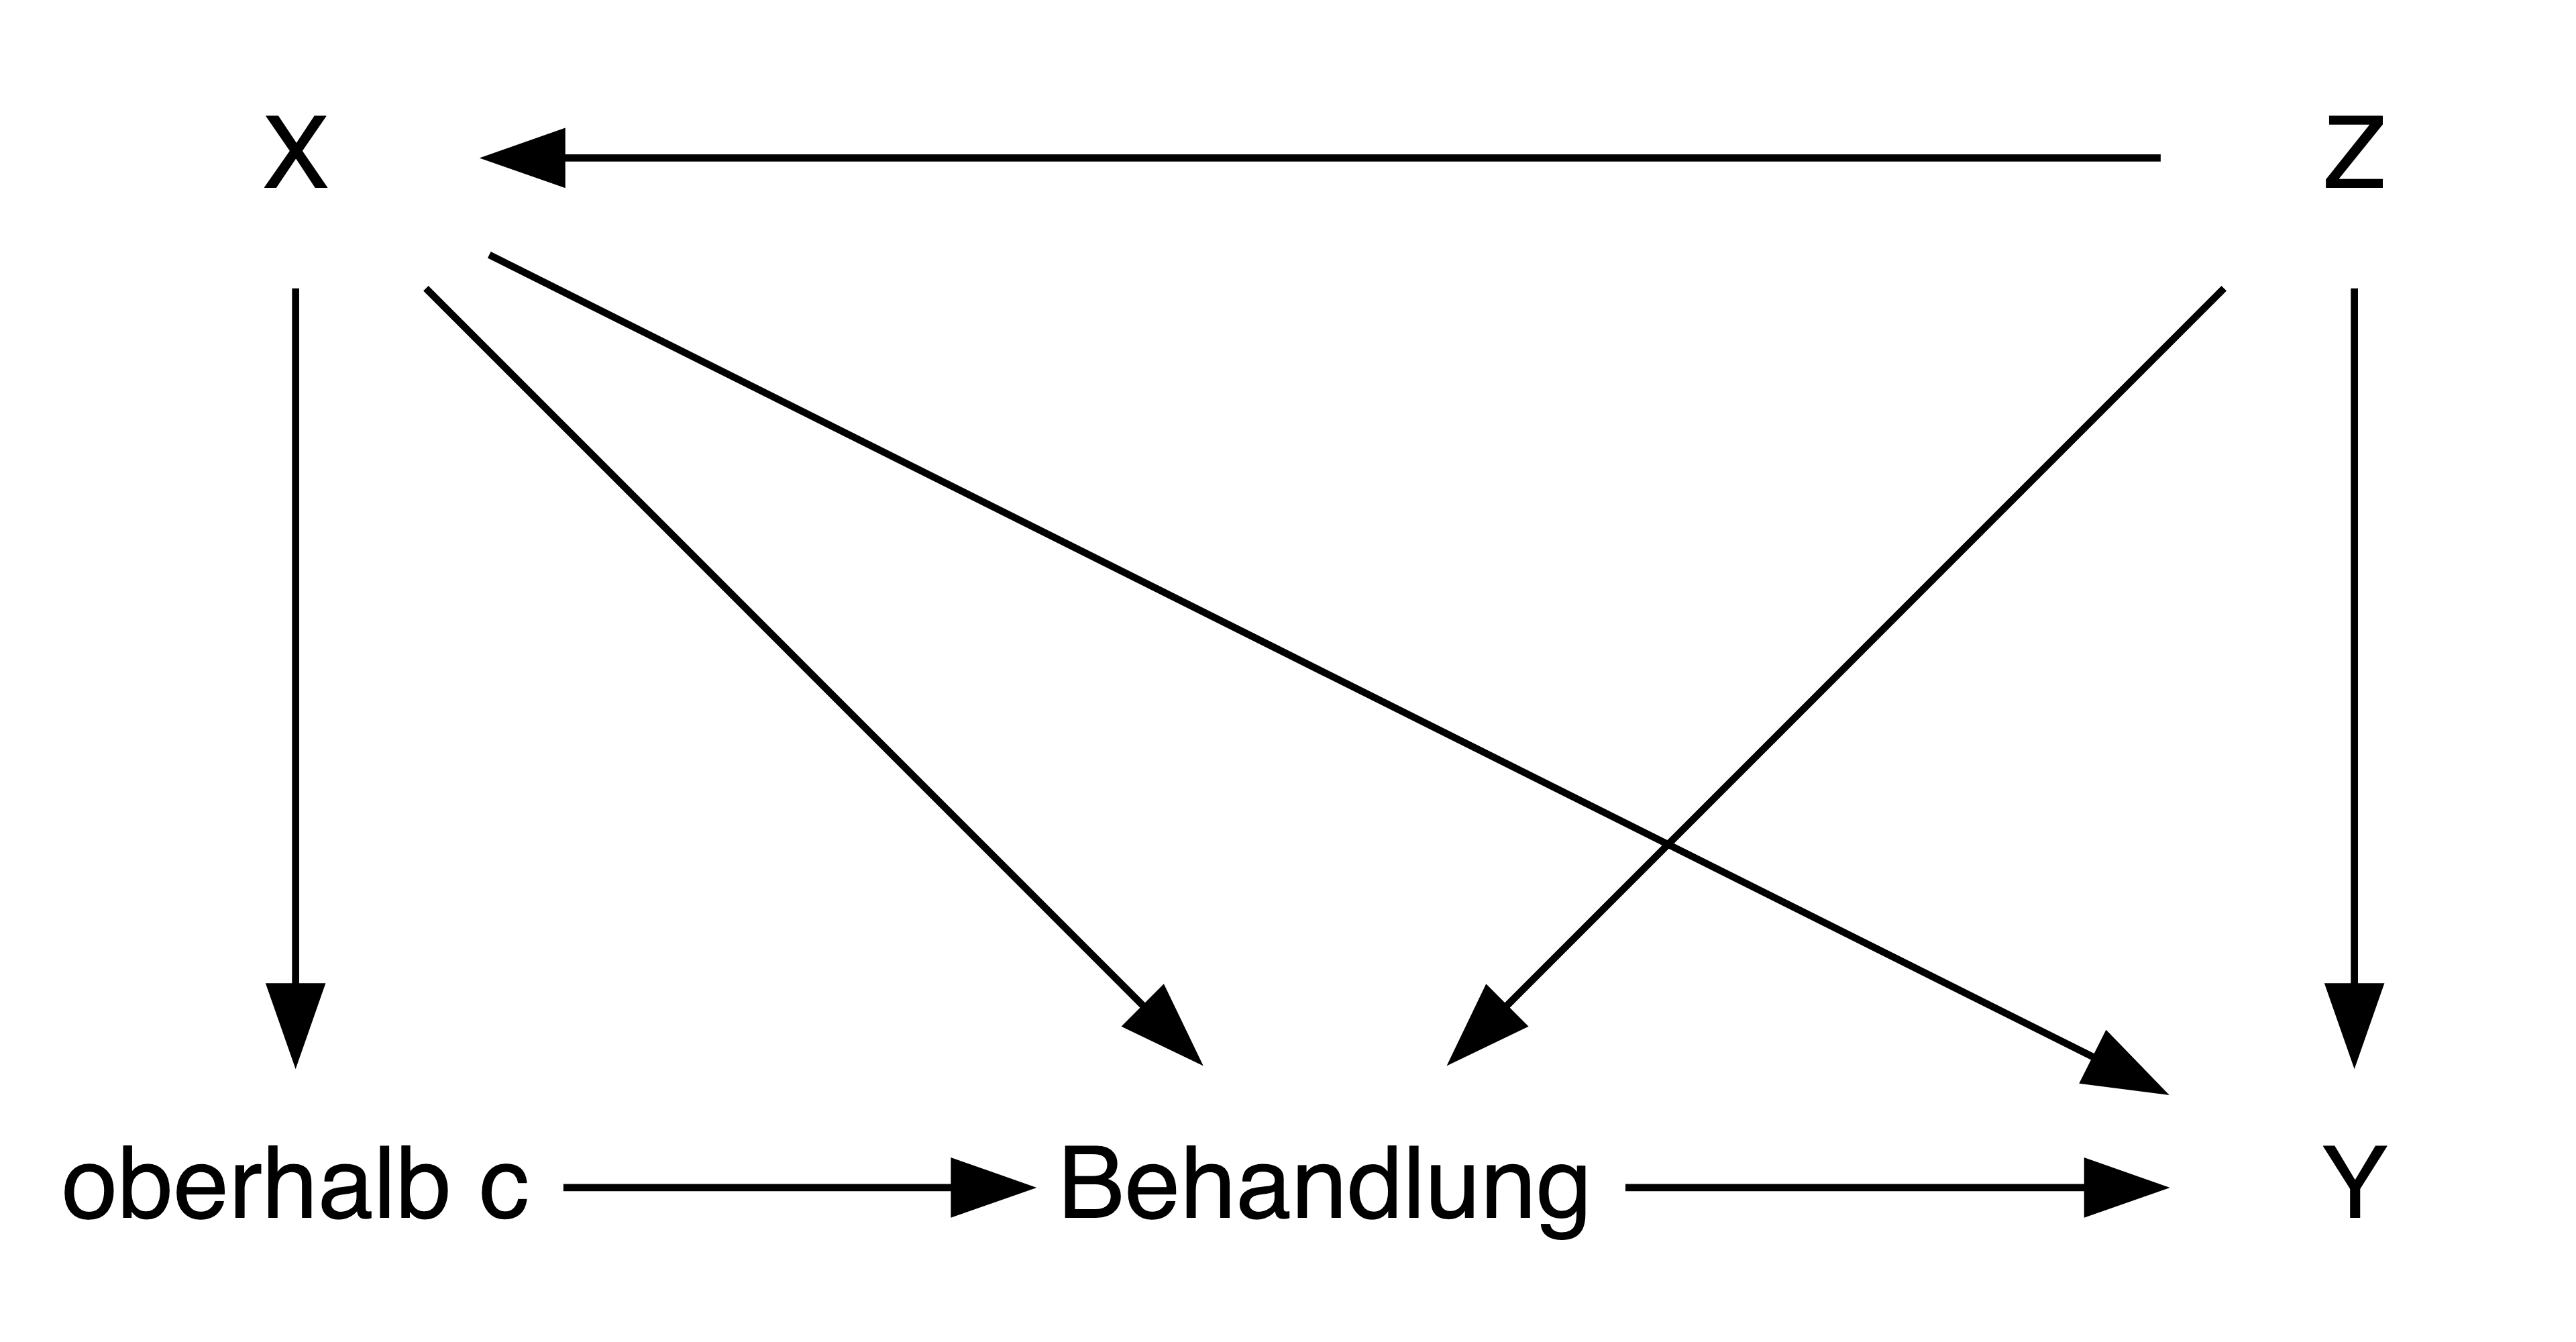
\includegraphics[width=5in,height=3in]{RDD_files/figure-latex/dot-figure-2.png}

}

\caption{\label{fig-CDFRDD}Kausales Diagram für FRDD}

\end{figure}%

Ein FRDD liegt vor, wenn die Zuweisung der Behandlung \(B\) durch die
Laufvariable \(X\) (und möglicherweise weitere Variablen \(Z\))
beeinflusst wird. Im Vergleich zum SRDD ist die Behandlung dann also
\emph{nicht} ausschließlich durch Überschreiten des Schwellenwerts
\(X = c\) bestimmt.

Abbildung~\ref{fig-CDFRDD} zeigt den grundsätzlichen Zusammenhang. Hier
genügt es weiterhin für \(X\) (und ggf. \(Z\)) zu kontrollieren, um den
Pfad \emph{oberhalb \(C\) → Behandlung \(B\) → \(Y\)} zu isolieren. Der
so für \emph{Behandlung \(B\)} ermittelte Effekt auf \(Y\) entspricht
jedoch \emph{nicht} dem ``vollständigen'' Behandlungseffekt, da bei
\(c\) die Zuweisung der Behandlung nicht von \(0\) auf \(100\%\)
springt. Die Schätzung des FRDD berücksichtigt dies und skaliert den
geschätzten Effekt entsprechend.

Wir betrachten zunächst den Zusammenhang \begin{align}
  Y_i = \beta_0 + \beta_1 B_i + \beta_2 (X_i - c) + u_i.\label{eq-simpleFRDD}
\end{align} In einem FRDD springt die Behandlungswahrscheinlichkeit am
Schwellenwert \(c\) um \(\Delta p<1\). Wir können \(B\) also nicht als
deterministische Funktion von \(X\), welche die Zuweisung zu
Behandlungs- bzw. Kontrollgruppe am Schwellenwert \(c\) anzeigt (wie im
SRDD), definieren. Stattdessen betrachten wir \begin{align}
  P(B_i=1\vert X_i) = 
  \begin{cases}
    g_{X_i<c}(X_i), & X_i < c \\ 
    g_{X_i\geq c}(X_i) & X_i \geq c
  \end{cases}\,. \label{eq-BFRDD}
\end{align} Die Funktionen \(g_{X_i<c}\) und \(g_{X_i\geq c}\) können
verschieden sein. Es muss jedoch
\[g_{X_i<c}(X_i = c) \neq g_{X_i\geq c}(X_i = c)\] gelten. Die
Behandlungsvariable \(B_i\) ist im FRDD also eine (binäre)
Zufallsvariable, deren bedingte Wahrscheinlichkeitsfunktion
\(P(B_i=1\vert X_i)\) am Schwellenwert \(c\) eine Diskontinuität
aufweist. Abbildung~\ref{fig-FRDDprobD} zeigt heispielhafte Verläufe
nicht-linearer bedingter Wahrscheinlichkeitsfunktion für die Behandlung
mit einer Diskontinuität bei \(X_i = c\).

\begin{Shaded}
\begin{Highlighting}[]
\FunctionTok{library}\NormalTok{(ggplot2)}
\FunctionTok{library}\NormalTok{(cowplot)}

\CommentTok{\# Bedingte Behandlungswahrscheinlichkeit im FRDD illustrieren}
\FunctionTok{ggplot}\NormalTok{() }\SpecialCharTok{+} 
  \FunctionTok{geom\_function}\NormalTok{(}
    \AttributeTok{fun =} \SpecialCharTok{\textasciitilde{}} \FunctionTok{ifelse}\NormalTok{(}
\NormalTok{      . }\SpecialCharTok{\textless{}} \DecValTok{0}\NormalTok{, }
      \SpecialCharTok{{-}}\NormalTok{.}\DecValTok{1} \SpecialCharTok{*}\NormalTok{ .}\SpecialCharTok{\^{}}\DecValTok{2} \SpecialCharTok{+}\NormalTok{ .}\DecValTok{25}\NormalTok{, }
      \SpecialCharTok{{-}}\NormalTok{.}\DecValTok{1} \SpecialCharTok{*}\NormalTok{ (.}\SpecialCharTok{{-}}\FloatTok{1.5}\NormalTok{)}\SpecialCharTok{\^{}}\DecValTok{2} \SpecialCharTok{+} \DecValTok{1}
\NormalTok{    ), }
    \AttributeTok{n =} \DecValTok{1000}
\NormalTok{  ) }\SpecialCharTok{+} 
    \FunctionTok{geom\_function}\NormalTok{(}
    \AttributeTok{fun =} \SpecialCharTok{\textasciitilde{}} \FunctionTok{ifelse}\NormalTok{(}
\NormalTok{      . }\SpecialCharTok{\textless{}} \DecValTok{0}\NormalTok{, }
\NormalTok{     .}\DecValTok{35}\NormalTok{, }
\NormalTok{     .}\DecValTok{65}
\NormalTok{    ),}
    \AttributeTok{n =} \DecValTok{1000}\NormalTok{, }
    \AttributeTok{lty =} \DecValTok{2}\NormalTok{, }
    \AttributeTok{col =} \StringTok{"red"}
\NormalTok{  ) }\SpecialCharTok{+} 
  \FunctionTok{scale\_x\_continuous}\NormalTok{(}
    \AttributeTok{name =} \StringTok{"Laufvariable X"}\NormalTok{, }
    \AttributeTok{limits =} \FunctionTok{c}\NormalTok{(}\SpecialCharTok{{-}}\FloatTok{1.5}\NormalTok{, }\FloatTok{1.5}\NormalTok{),}
    \AttributeTok{labels =} \ConstantTok{NULL}\NormalTok{,}
    \AttributeTok{breaks =} \ConstantTok{NULL}
\NormalTok{  ) }\SpecialCharTok{+}
  \FunctionTok{scale\_y\_continuous}\NormalTok{(}
    \AttributeTok{name =} \StringTok{"P(D=1|X)"}\NormalTok{, }
    \AttributeTok{breaks =} \FunctionTok{c}\NormalTok{(}\DecValTok{0}\NormalTok{, }\DecValTok{1}\NormalTok{), }
    \AttributeTok{limits =} \FunctionTok{c}\NormalTok{(}\DecValTok{0}\NormalTok{, }\DecValTok{1}\NormalTok{)}
\NormalTok{  ) }\SpecialCharTok{+}
  \FunctionTok{theme\_cowplot}\NormalTok{()}
\end{Highlighting}
\end{Shaded}

\begin{figure}[t]

\centering{

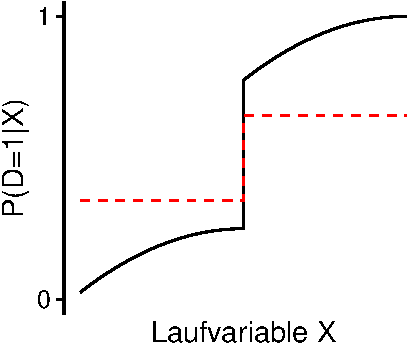
\includegraphics{RDD_files/figure-pdf/fig-FRDDprobD-1.pdf}

}

\caption{\label{fig-FRDDprobD}Bedingte Behandlungswahrscheinlichkeiten
im FRDD}

\end{figure}%

Definition \eqref{eq-BFRDD} bedeutet, dass eine KQ-Schätzung von
\(\beta_1\) anhand \eqref{eq-simpleFRDD} eine \emph{verzerrte} Schätzung
des Behandlungseffekts ist: Der in \(\widehat{\beta}_1\) erfasste Effekt
auf \(Y\) ist auf einen Sprung der Behandlungswahrscheinlichkeit bei
\(X_i = c\) um \emph{weniger} als \(100\%\) zurückzuführen. Der wahre
Behandlungseffekt wird also \emph{unterschätzt}. Daher muss
\(\widehat{\beta}_1\) skaliert werden, sodass die Schätzung als Effekt
einer Änderung der Behandlungswahrscheinlichkei um \(100\%\)
interpretiert werden kann --- der erwartete Effekt, wenn ausschließlich
Subjekte mit \(X_i\geq c\) behandelt würden. Diese skalierte Schätzung
erhalten wir mit IV-Regression (vgl. Kapitel XYZ). Hierfür nutzen wir
für \(B_i\) die Instrumentvariable \begin{align*}
  D_i = \begin{cases}
    0, & X_i < c \\ 
    1, & X_i \geq c.
  \end{cases}
\end{align*}

Angenommen \(g_{X_i\geq c}(X_i) = \alpha_0\) und
\(g_{X_i<c}(X_i) = \alpha_0 + \alpha_1\) mit \(\alpha_0 + \alpha_1 < 1\)
(vgl. rote Funktion in Abbildung~\ref{fig-CDFRDD}). Der FRDD-Schätzer
des Behandlungseffekts ist dann \(\widehat{\gamma}_\textup{FRDD}\) im
2SLS-Verfahren mit den Regressionen \begin{align}
  \begin{split}
  (\mathrm{I})\qquad B_i =&\, \alpha_0 + \alpha_1 D_i + \alpha_2 (X_i - c) + e_i,\\
  (\mathrm{II})\qquad Y_i =&\, \gamma_0 + \gamma_1 \widehat{B}_i + \gamma_2 (X_i - c) + \epsilon_i,
  \end{split}\label{eq:FRDD_simpleIV}
\end{align} wobei \(\widehat{B}_i\) die angepassten Werte aus Stufe
\((\mathrm I)\) und \(e_i\) sowie \(\epsilon_i\) Fehlterterme sind.

Analog zum SRDD müssen in empirischen Anwendungen geeignete
Spezifikationen für die Regressionsfunktionen \eqref{eq-simpleFRDD} und
\eqref{eq-BFRDD} gewählt und der 2SLS-Schätzer \eqref{eq:FRDD_simpleIV}
entsprechend angepasst werden. Ein einfaches Interaktionsmodell wäre
\begin{align}
  \begin{split}
  (\mathrm{I})\qquad B_i =&\, \alpha_0 + \alpha_1 D_i + \alpha_2 (X_i - c)\\ 
  +&\, \alpha_3 (X_i - c) \times D_i + e_i,\\
  \\
  (\mathrm{II})\qquad Y_i =&\, \gamma_0 + \gamma_1 \widehat{B}_i\\
  +&\, \gamma_2 (X_i - c) + \gamma_3 (X_i-c)\times\widehat{B}_i, \epsilon_i
  \end{split},\label{eq:FRDD_lintIV}
\end{align} d.h. wir instrumentieren \(B_i\) mit \(D_i\) und dem
Interaktionsterm \((X_i-c)\times D_i\).

Wie im SRDD werden die IV-Ansätze für das FRDD \eqref{eq:FRDD_simpleIV}
und \eqref{eq:FRDD_lintIV} in empirischen Studien unter Berücksichtigung
einer Bandweite (i.d.R. dieselbe Bandweite für beide Stufen) angewendet.

\section{Case Study: Protestantische
Arbeitsethik}\label{case-study-protestantische-arbeitsethik}

Die Studie \emph{Beyond Work Ethic: Religion, Individual, and Political
Preferences} (Basten und Betz 2013) untersucht den Zusammenhang zwischen
Religion, individuellen Merkmalen und politischen Präferenzen. Das
Hauptaugenmerk ist die Rolle von Religiosität als Einflussfaktor auf
politische Einstellungen. Die Hypothese der Autoren ist, dass
Religiosität eines Individuums über den traditionellen Rahmen von
Moralvorstellungen und sozialen Normen hinaus auch die politischen
Präferenzen beeinflusst. Eine entsprechende Theorie wurde zu Beginn des
20. Jahrhunderts entwickelt und prominent von Max Weber (vgl. Weber
2004) vertreten. Weber argumentiert, dass die protestantische
Arbeitsethik einen entscheidenden Einfluss auf die Entwicklung des
Kapitalismus hatte. Laut Weber führte der protestantische Glaube an
harte Arbeit, ein sparsames Leben und ethisches Verhalten zur einer in
den damaligen Gesellschaften weit verbreiteten Geisteshaltung, die
wirtschaftliches Wachstum förderte und den Aufstieg des Kapitalismus
begünstigte.

Basten und Betz (2013) nutzen Wahlergebnisse sowie geo- und
soziodemographische Datensätze für schweizer Gemeinden, um den
Zusammenhang zwischen Religiosität und politischen Präferenzen wie
links-rechts-Ausrichtung, Einstellungen zur Umverteilung und
Einwanderung zu untersuchen. Hierfür verwenden die Autoren ein FRDD,
dass eine historisch bedingte Diskontinuität der geographischen
Verteilung von evanglischer bzw. katholischer Religionszugehörigkeit
zwischen den Kantonen Freiburg (überwiegend dunkelrote Region, frz.
\emph{Fribourg}) und Waadt (kleinere hellrote Region, frz. \emph{Vaud})
ausnutzt. Die historische Verteilung der Konfessionen in der
betrachteten Region im 16. Jahrhundert durch Abspaltung des Kantons
Freiburg ist in Abbildung~\ref{fig-vaudfb} dargestellt.

Aufgrund von Bevölkerungsbewegungen ist die Verteilung der Konfessionen
zwar nicht mehr eindeutig durch die Kantonsgrenze bestimmt, jedoch sind
die Gemeinden der betrachteten Kantone auch heute noch mehrheitlich
protestantisch bzw. katholisch. Es ist plausibel, dass eine Prägung
gemäß Webers Theorie vorliegt, sich die Gemeinden nahe der Grenz aber
hinsichtlich anderer Charakteristika (insb. der Bevölkerungsstruktur)
nicht systematisch unterscheiden. Somit liegt ein quai

{
\makeatletter
\def\LT@makecaption#1#2#3{%
  \noalign{\smash{\hbox{\kern\textwidth\rlap{\kern\marginparsep
  \parbox[t]{\marginparwidth}{%
    \footnotesize{%
      \vspace{(1.1\baselineskip)}
    #1{#2: }\ignorespaces #3}}}}}}%
    }
\makeatother

\begin{figure}[t]

\sidecaption{\label{fig-vaudfb}Historische Verteilung von
Religionszugehörigkeit in Schweizer Gemeinden im 16. Jahrhundert.
Quelle: Basten und Betz (2013).}

\centering{

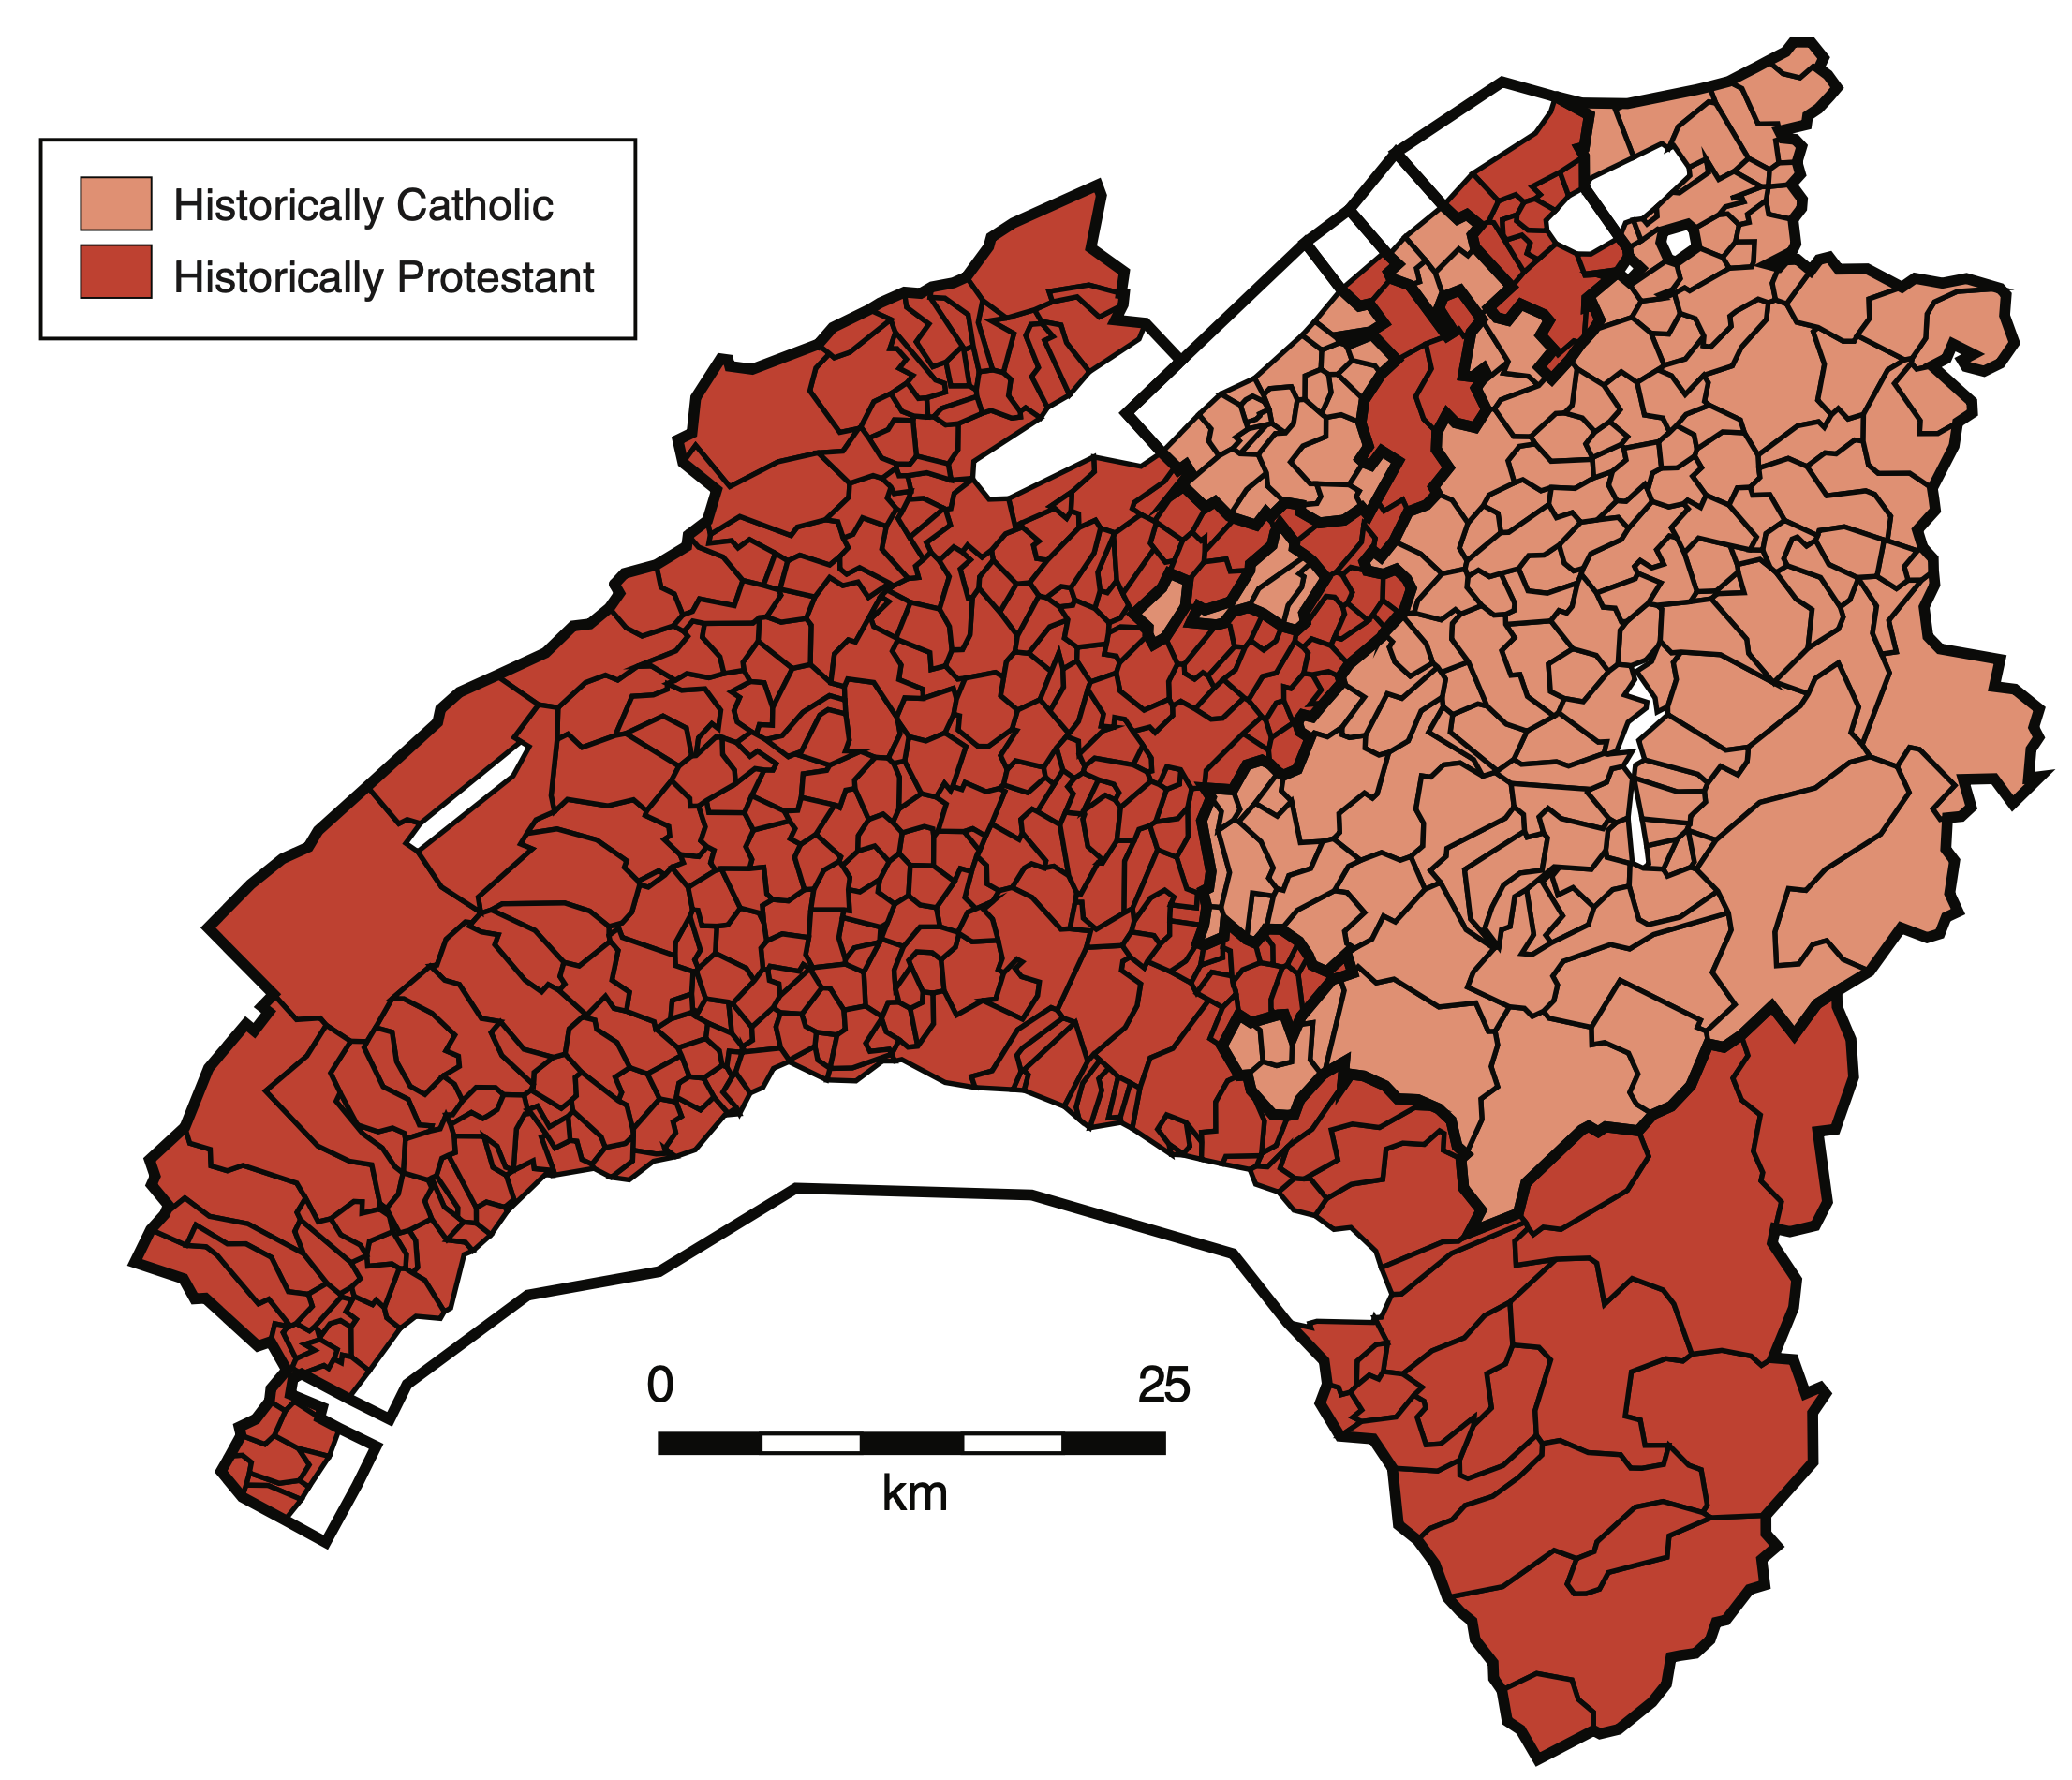
\includegraphics[width=4.16667in,height=\textheight]{img/WaadtFribourg.png}

}

\end{figure}%

}

Die Ergebnisse der Studie zeigen einen signifikanten Einfluss von
Protestantismus auf politische Präferenzen, die über traditionelle
Moralvorstellungen hinausgehen: Die Autoren finden Hinweise, dass
Einwohner evangelisch geprägter Gemeinden eher konservative soziale und
politische Ansichten vertreten. Eine mögliche Erklärung für diesen
Effekt ist, dass religiöse Institutionen auch eine soziale und
politische Agenda verfolgen, die von den Gläubigen internalisiert wird.

\subsection{Aufbereitung der Daten}\label{aufbereitung-der-daten}

In diesem Kapitel zeigen wir, wie die Kernergebnisse der Studie mit R
reproduziert werden können. Hierfür werden folgende Pakete benötigt.

\begin{Shaded}
\begin{Highlighting}[]
\FunctionTok{library}\NormalTok{(tidyverse)}
\FunctionTok{library}\NormalTok{(haven)}
\FunctionTok{library}\NormalTok{(vtable)}
\FunctionTok{library}\NormalTok{(rdrobust)}
\end{Highlighting}
\end{Shaded}

Das Papier sowie der Datensatz \texttt{BastenBetz.dta} sind auf der
\href{https://www.aeaweb.org/articles?id=10.1257/pol.5.3.67}{Übersichtsseite
der AEA} verfügbar und liegt im STATA-Format \texttt{.dta}
vor.\footnote{Siehe alternativ das
  \href{https://papers.ssrn.com/sol3/papers.cfm?abstract_id=2133848}{working
  paper}, falls kein Abbonement für AEA-Journals vorliegt.}

\begin{Shaded}
\begin{Highlighting}[]
\CommentTok{\# Datensatz einlesen}
\NormalTok{BastenBetz }\OtherTok{\textless{}{-}} \FunctionTok{read\_dta}\NormalTok{(}\StringTok{\textquotesingle{}BastenBetz.dta\textquotesingle{}}\NormalTok{)}
\end{Highlighting}
\end{Shaded}

Der Datensatz \texttt{BastenBetz} enthält Beobachtungen zu 509 schweizer
Gemeinden. Eine Vielzahl an Variablen ist lediglich für
Robustheits-Checks relevant. Für die Reproduktion der Kernergebnisse
erstellen wir zunächst einen reduzierten Datensatz und transformieren
einige Variablen.

\begin{Shaded}
\begin{Highlighting}[]
\CommentTok{\# Reduzierten Datensatz erstellen}
\NormalTok{BastenBetz }\OtherTok{\textless{}{-}}\NormalTok{ BastenBetz }\SpecialCharTok{\%\textgreater{}\%}
  \FunctionTok{transmute}\NormalTok{(}
    \AttributeTok{gini =}\NormalTok{ Ecoplan\_gini,}
    \AttributeTok{prot =}\NormalTok{ prot1980s,}
    \AttributeTok{bord =}\NormalTok{ borderdis, }
\NormalTok{    vaud,}
\NormalTok{    pfl, }
\NormalTok{    pfr, }
\NormalTok{    pfi}
\NormalTok{  )}
\end{Highlighting}
\end{Shaded}

Die Definitionen der Variablen sind in Tabelle~\ref{tbl-BastenBetzRed}
gegeben. Die Präferenzen \texttt{pfl}, \texttt{pfr} und \texttt{pfi}
basieren auf Wahlergebnissen auf Gemeindeebene zu Volksentscheiden.

\begin{longtable}[]{@{}
  >{\raggedright\arraybackslash}p{(\columnwidth - 2\tabcolsep) * \real{0.1806}}
  >{\raggedright\arraybackslash}p{(\columnwidth - 2\tabcolsep) * \real{0.8194}}@{}}
\caption{\texttt{BastenBetz} -- Variablen und
Definitionen}\label{tbl-BastenBetzRed}\tabularnewline
\toprule\noalign{}
\begin{minipage}[b]{\linewidth}\raggedright
Variable
\end{minipage} & \begin{minipage}[b]{\linewidth}\raggedright
Definition
\end{minipage} \\
\midrule\noalign{}
\endfirsthead
\toprule\noalign{}
\begin{minipage}[b]{\linewidth}\raggedright
Variable
\end{minipage} & \begin{minipage}[b]{\linewidth}\raggedright
Definition
\end{minipage} \\
\midrule\noalign{}
\endhead
\bottomrule\noalign{}
\endlastfoot
\texttt{prot} & Anteil Prothestanten im Jahr 1980 (\%) \\
\texttt{gini} & Gini-Koeffizient \\
\texttt{bord} & Laufdistanz zur Kantonsgrenze (Km) \\
\texttt{vaud} & Dummyvariable: Gemeine im Kanton Waadt \\
\texttt{pfl} & Präferenz für Freizeit (\%) \\
\texttt{pfr} & Präferenz für Umverteilung (\%) \\
\texttt{pfi} & Präferenz für wirtschaftliche Intervention des Staats
(\%) \\
\end{longtable}

Für die Berechnung der optimalen Bandweite des FRDD verwenden wir einen
MSE-optimalen Schätzer, der in der Funktion
\texttt{rdrobust::rdbwselect()} implementiert ist.\footnote{Basten und
  Betz (2013) setzen BW = 5.01, den Durchschnitt von IK-Schätzungen über
  Modelle sämtlicher betrachteter Outcome-Variablen. Diese Bandweite
  liegt nahe des Ergebnisses von \texttt{rdbwselect}. Wir verwenden
  nachfolgend die Schätzung \texttt{OB}.}

\begin{Shaded}
\begin{Highlighting}[]
\CommentTok{\# Bandweite schätzen (Bsp. für Freizeitpräferenz)}
\NormalTok{bw\_selection }\OtherTok{\textless{}{-}} \FunctionTok{rdbwselect}\NormalTok{(}
  \AttributeTok{y =}\NormalTok{ BastenBetz}\SpecialCharTok{$}\NormalTok{pfl,}
  \AttributeTok{x =}\NormalTok{ BastenBetz}\SpecialCharTok{$}\NormalTok{bord,}
  \AttributeTok{fuzzy =}\NormalTok{ BastenBetz}\SpecialCharTok{$}\NormalTok{prot, }
  \AttributeTok{bwselect =} \StringTok{"mserd"}\NormalTok{, }
  \AttributeTok{kernel =} \StringTok{"uniform"}
\NormalTok{) }

\CommentTok{\# Bandweite auslesen und zuweisen}
\NormalTok{(OB }\OtherTok{\textless{}{-}}\NormalTok{ bw\_selection}\SpecialCharTok{$}\NormalTok{bws[}\DecValTok{1}\NormalTok{])}
\end{Highlighting}
\end{Shaded}

\begin{verbatim}
[1] 5.078001
\end{verbatim}

\subsection{Deskriptive Statistiken}\label{deskriptive-statistiken}

Zur Reproduktion von Tabelle 1 aus Basten und Betz (2013) erzeugen wir
eine nach Kantonen gruppierte Zusammenfassung der Daten und berechnen
deskriptive Statistiken. Wie im Paper berücksichtigen wir hierbei nur
Gemeinden innerhalb der geschätzten optimalen Bandweite \texttt{OB}.

\begin{Shaded}
\begin{Highlighting}[]
\CommentTok{\# Datensatz für Reproduktion von Table 1 formatieren}
\NormalTok{T1 }\OtherTok{\textless{}{-}}\NormalTok{ BastenBetz }\SpecialCharTok{\%\textgreater{}\%}
  \FunctionTok{filter}\NormalTok{(}\FunctionTok{abs}\NormalTok{(bord) }\SpecialCharTok{\textless{}}\NormalTok{ OB) }\SpecialCharTok{\%\textgreater{}\%}
  \FunctionTok{mutate}\NormalTok{(}
    \AttributeTok{vaud =} \FunctionTok{ifelse}\NormalTok{(}
      \AttributeTok{test =}\NormalTok{ vaud }\SpecialCharTok{==} \DecValTok{1}\NormalTok{, }
      \AttributeTok{yes =} \StringTok{"Waadt"}\NormalTok{, }
      \AttributeTok{no =} \StringTok{"Freiburg"}
\NormalTok{    ),}
    \AttributeTok{prot =}\NormalTok{ prot }\SpecialCharTok{*} \DecValTok{100}
\NormalTok{  ) }\SpecialCharTok{\%\textgreater{}\%}
  \FunctionTok{group\_by}\NormalTok{(vaud) }\SpecialCharTok{\%\textgreater{}\%}
  \FunctionTok{summarise}\NormalTok{(}
    \FunctionTok{across}\NormalTok{(}
      \FunctionTok{everything}\NormalTok{(), }
      \FunctionTok{list}\NormalTok{(}
        \AttributeTok{Mean =}\NormalTok{ mean, }
        \AttributeTok{SD =}\NormalTok{ sd, }
        \AttributeTok{N =}\NormalTok{ length}
\NormalTok{      )}
\NormalTok{    )}
\NormalTok{  ) }\SpecialCharTok{\%\textgreater{}\%}
  \FunctionTok{pivot\_longer}\NormalTok{(}
    \AttributeTok{cols =} \SpecialCharTok{{-}}\NormalTok{vaud,}
    \AttributeTok{names\_to =} \FunctionTok{c}\NormalTok{(}\StringTok{"variable"}\NormalTok{, }\StringTok{"statistic"}\NormalTok{), }
    \AttributeTok{names\_sep =} \StringTok{"\_"}
\NormalTok{  )}
\end{Highlighting}
\end{Shaded}

Für die tabellarische Darstellung transformieren wir in ein weites
Format, sodass die Tabelle die deskriptive Statistiken spaltenweise für
die Kantone zeigt.

\begin{Shaded}
\begin{Highlighting}[]
\CommentTok{\# Daten in weites Format überführen}
\NormalTok{T1\_wider }\OtherTok{\textless{}{-}}\NormalTok{ T1 }\SpecialCharTok{\%\textgreater{}\%} 
  \FunctionTok{pivot\_wider}\NormalTok{(}
    \AttributeTok{names\_from =} \FunctionTok{c}\NormalTok{(}\StringTok{"vaud"}\NormalTok{, }\StringTok{"statistic"}\NormalTok{)}
\NormalTok{  )}
\end{Highlighting}
\end{Shaded}

Die Tabelle erzeugen wir mit \texttt{gt::gt()}.

\begin{Shaded}
\begin{Highlighting}[]
\CommentTok{\# Tabelle mit gt() erzeugen}
\NormalTok{T1\_wider }\SpecialCharTok{\%\textgreater{}\%}
  \FunctionTok{gt}\NormalTok{(}\AttributeTok{rowname\_col =} \StringTok{"Variable"}\NormalTok{) }\SpecialCharTok{\%\textgreater{}\%} 
  \FunctionTok{tab\_spanner\_delim}\NormalTok{(}
    \AttributeTok{delim =} \StringTok{"\_"}\NormalTok{,}
\NormalTok{  ) }\SpecialCharTok{\%\textgreater{}\%}
\NormalTok{ tabopts}
\end{Highlighting}
\end{Shaded}

\begin{longtable}{lrrrrrr}

\caption{\label{tbl-sumstat}Datensatz \texttt{BastenBetz} --
Zusammenfassende Statistiken}

\tabularnewline

\toprule
 & \multicolumn{3}{c}{Freiburg} & \multicolumn{3}{c}{Waadt} \\ 
\cmidrule(lr){2-4} \cmidrule(lr){5-7}
variable & Mean & SD & N & Mean & SD & N \\ 
\midrule\addlinespace[2.5pt]
gini & $0.302$ & $0.029$ & $49$ & $0.367$ & $0.052$ & $84$ \\ 
prot & $9.428$ & $5.695$ & $49$ & $83.245$ & $11.411$ & $84$ \\ 
bord & $-2.327$ & $1.274$ & $49$ & $2.493$ & $1.201$ & $84$ \\ 
pfl & $48.239$ & $4.774$ & $49$ & $39.508$ & $5.723$ & $84$ \\ 
pfr & $43.049$ & $2.634$ & $49$ & $39.19$ & $5.025$ & $84$ \\ 
pfi & $52.642$ & $2.94$ & $49$ & $47.086$ & $3.368$ & $84$ \\ 
\bottomrule

\end{longtable}

Die Statistiken in Tabelle~\ref{tbl-sumstat} scheinen konsistent mit der
(historischen) Verteilung der Religionszugehörigkeit und politischen
Einstellung gemäß der Hypothese: Im überwiegend katholischen Freiburg
finden wir eine größere Einkommensungleichkeit und höhere aus
Wahlergebnissen abgeleitete Präferenzen für Freizeit, Umverteilung sowie
staatliche Interventionen.

\subsection{Modellspezifikation und
First-Stage-Ergebnisse}\label{modellspezifikation-und-first-stage-ergebnisse}

\begin{Shaded}
\begin{Highlighting}[]
\NormalTok{CJM\_BB }\OtherTok{\textless{}{-}} \FunctionTok{rddensity}\NormalTok{(BastenBetz}\SpecialCharTok{$}\NormalTok{bord, }\AttributeTok{c =} \DecValTok{0}\NormalTok{, }\AttributeTok{kernel =} \StringTok{"epanechnikov"}\NormalTok{)}
\FunctionTok{summary}\NormalTok{(CJM\_BB)}
\end{Highlighting}
\end{Shaded}

\begin{verbatim}

Manipulation testing using local polynomial density estimation.

Number of obs =       509
Model =               unrestricted
Kernel =              epanechnikov
BW method =           estimated
VCE method =          jackknife

c = 0                 Left of c           Right of c          
Number of obs         127                 382                 
Eff. Number of obs    69                  124                 
Order est. (p)        2                   2                   
Order bias (q)        3                   3                   
BW est. (h)           8.531               9.57                

Method                T                   P > |T|             
Robust                0.7552              0.4501              


P-values of binomial tests (H0: p=0.5).

Window Length              <c     >=c    P>|T|
1.400     + 1.400          20      20    1.0000
2.192     + 2.308          27      47    0.0265
2.985     + 3.215          34      60    0.0095
3.777     + 4.123          40      72    0.0032
4.570     + 5.031          44      84    0.0005
5.362     + 5.939          51      95    0.0003
6.154     + 6.846          56     100    0.0005
6.947     + 7.754          60     106    0.0004
7.739     + 8.662          67     114    0.0006
8.531     + 9.570          69     124    0.0001
\end{verbatim}

\begin{Shaded}
\begin{Highlighting}[]
\CommentTok{\# CJM{-}Plot}
\NormalTok{plot }\OtherTok{\textless{}{-}} \FunctionTok{rdplotdensity}\NormalTok{(}
  \AttributeTok{rdd =}\NormalTok{ CJM\_BB,}
  \AttributeTok{X =}\NormalTok{ BastenBetz}\SpecialCharTok{$}\NormalTok{bord, }
  \AttributeTok{type =} \StringTok{"both"}\NormalTok{, }\AttributeTok{plotN =} \DecValTok{20}\NormalTok{, }
\NormalTok{)}
\end{Highlighting}
\end{Shaded}

\begin{center}
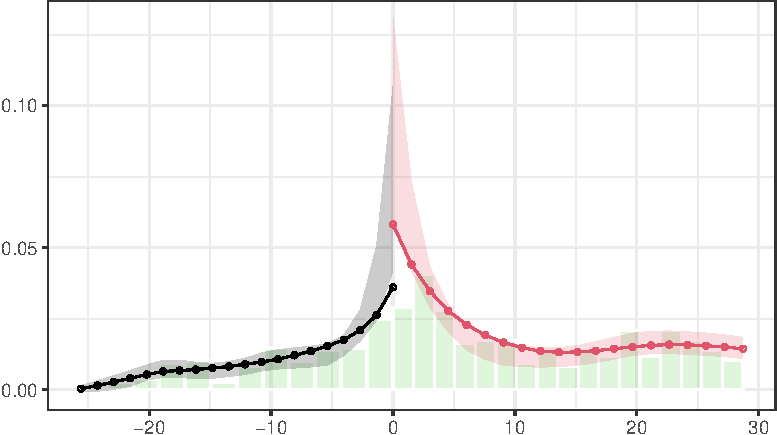
\includegraphics{RDD_files/figure-pdf/unnamed-chunk-38-1.pdf}
\end{center}

Die Kantone Waadt und Freiburg haben bis heute mehrheitlich
protestantische bzw. katholische Gemeinden. Die Verteilung von
Protestantismus ist also, u.a. aufgrund von Bevölkerungsbewegungen,
nicht mehr deterministisch. An der Kantonsgrenze besteht jedoch eine
deutliche Diskontinuität im Anteil protestantischer Einwohner, die auf
die historische Verteilung der Religionszugehörigkeit zurückzuführen
ist. Damit kann ein FRDD implementiert werden, bei dem die Distanz zur
Grenze (\texttt{bord}) die zentrierte Laufvariable ist und die
Zugehörigkeit zum Kanton Waadt (\texttt{vaud}) ein Instrument für die
Behandlungsvariable (\texttt{prot}) ist.

Wir nutzen die Funktion \texttt{rdrobust::rdplot} um diesen Zusammenhang
für verschiedene Bandweiten anhand des linearen Interaktionsmodells
\begin{align}
  \begin{split}
  prot_i =&\, \alpha_0 + \alpha_1 vaud_i + \alpha_2 bord_i \\
  +&\, \alpha_3 bord_i \times vaud_i + u_i
  \end{split}\label{eq:BBFSR}
\end{align} grafisch darzustellen. Dies ist die First-Stage-Regression
für die 2SLS-Schätzung der Behandlungseffekte.

\begin{Shaded}
\begin{Highlighting}[]
\CommentTok{\# Reproduktion von Abbildung 3 in Basten und Betz (2013)}
\NormalTok{plots\_BB }\OtherTok{\textless{}{-}} \FunctionTok{list}\NormalTok{(}
  \CommentTok{\# gesch. optimale Bandweite}
  \AttributeTok{p\_OB =} \FunctionTok{rdplot}\NormalTok{(}
    \AttributeTok{y =}\NormalTok{ BastenBetz}\SpecialCharTok{$}\NormalTok{prot, }
    \AttributeTok{x =}\NormalTok{ BastenBetz}\SpecialCharTok{$}\NormalTok{bord, }
    \AttributeTok{h =} \FunctionTok{c}\NormalTok{(OB, OB), }
    \AttributeTok{x.label =} \StringTok{"Distanz zur Grenze (bord)"}\NormalTok{,}
    \AttributeTok{y.label =} \StringTok{"Anteil Protestanten (prot)"}\NormalTok{, }
    \AttributeTok{title =} \StringTok{"Gesch. Bandweite"}\NormalTok{,}
    \AttributeTok{p =} \DecValTok{1}\NormalTok{, }
    \AttributeTok{nbins =} \FunctionTok{c}\NormalTok{(}\DecValTok{6}\NormalTok{, }\DecValTok{14}\NormalTok{), }
    \AttributeTok{masspoints =} \StringTok{"off"}
\NormalTok{  ),}
  
  \CommentTok{\# Bandweite 10}
  \AttributeTok{p\_BW10 =} \FunctionTok{rdplot}\NormalTok{(}
    \AttributeTok{y =}\NormalTok{ BastenBetz}\SpecialCharTok{$}\NormalTok{prot, }
    \AttributeTok{x =}\NormalTok{ BastenBetz}\SpecialCharTok{$}\NormalTok{bord, }
    \AttributeTok{h =} \FunctionTok{c}\NormalTok{(}\DecValTok{10}\NormalTok{, }\DecValTok{10}\NormalTok{), }
    \AttributeTok{x.label =} \StringTok{"Distanz zur Grenze (bord)"}\NormalTok{,}
    \AttributeTok{y.label =} \StringTok{"Anteil Protestanten  (prot)"}\NormalTok{, }
    \AttributeTok{title =} \StringTok{"Bandweite = 10"}\NormalTok{,}
    \AttributeTok{p =} \DecValTok{1}\NormalTok{, }
    \AttributeTok{nbins =} \FunctionTok{c}\NormalTok{(}\DecValTok{6}\NormalTok{, }\DecValTok{14}\NormalTok{),}
    \AttributeTok{masspoints =} \StringTok{"off"}
\NormalTok{  ),}
  
  \CommentTok{\# Bandweite 20}
  \AttributeTok{p\_BW20 =} \FunctionTok{rdplot}\NormalTok{(}
    \AttributeTok{y =}\NormalTok{ BastenBetz}\SpecialCharTok{$}\NormalTok{prot, }
    \AttributeTok{x =}\NormalTok{ BastenBetz}\SpecialCharTok{$}\NormalTok{bord, }
    \AttributeTok{h =} \FunctionTok{c}\NormalTok{(}\DecValTok{20}\NormalTok{, }\DecValTok{20}\NormalTok{), }
    \AttributeTok{x.label =} \StringTok{"Distanz zur Grenze (bord)"}\NormalTok{,}
    \AttributeTok{y.label =} \StringTok{"Anteil Protestanten  (prot)"}\NormalTok{, }
    \AttributeTok{title =} \StringTok{"Bandweite = 20"}\NormalTok{,}
    \AttributeTok{p =} \DecValTok{1}\NormalTok{, }
    \AttributeTok{nbins =} \FunctionTok{c}\NormalTok{(}\DecValTok{6}\NormalTok{, }\DecValTok{14}\NormalTok{),}
    \AttributeTok{masspoints =} \StringTok{"off"}
\NormalTok{  ),}
  
  \CommentTok{\# Gesamter Datensatz}
  \AttributeTok{p\_G =} \FunctionTok{rdplot}\NormalTok{(}
    \AttributeTok{y =}\NormalTok{ BastenBetz}\SpecialCharTok{$}\NormalTok{prot, }
    \AttributeTok{x =}\NormalTok{ BastenBetz}\SpecialCharTok{$}\NormalTok{bord,}
    \AttributeTok{x.label =} \StringTok{"Distanz zur Grenze (bord)"}\NormalTok{,}
    \AttributeTok{y.label =} \StringTok{"Anteil Protestanten"}\NormalTok{, }
    \AttributeTok{title =} \StringTok{"Ges. Datensatz"}\NormalTok{,}
    \AttributeTok{p =} \DecValTok{1}\NormalTok{, }
    \AttributeTok{nbins =} \FunctionTok{c}\NormalTok{(}\DecValTok{6}\NormalTok{, }\DecValTok{14}\NormalTok{),}
    \AttributeTok{masspoints =} \StringTok{"off"}
\NormalTok{  )}
\NormalTok{)}
\end{Highlighting}
\end{Shaded}

Wir sammeln die Ergebnisse in einem Plot-Gitter mit
\texttt{cowplot::plot\_grid()}.

\begin{Shaded}
\begin{Highlighting}[]
\CommentTok{\# Reproduktion von Abbildung 3 in Basten und Betz (2013)}
\FunctionTok{plot\_grid}\NormalTok{(}
  \AttributeTok{plotlist =} \FunctionTok{map}\NormalTok{(plots\_BB, }\SpecialCharTok{\textasciitilde{}}\NormalTok{ .}\SpecialCharTok{$}\NormalTok{rdplot), }\AttributeTok{ncol =} \DecValTok{2}
\NormalTok{)}
\end{Highlighting}
\end{Shaded}

\begin{figure}[t]

\sidecaption{\label{fig-BastenBetzFS}First-Stage-Regressionen}

\centering{

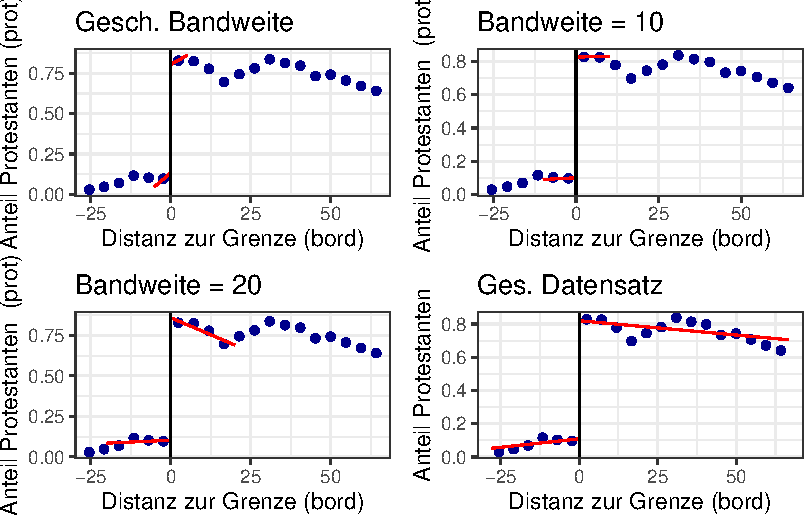
\includegraphics{RDD_files/figure-pdf/fig-BastenBetzFS-1.pdf}

}

\end{figure}%

Die Grafiken in Abbildung~\ref{fig-BastenBetzFS} zeigen deutliche
Hinweise auf die Diskontinuität in \texttt{prot} nahe der Kantonsgrenze.
Die Größe des geschätzten Sprungs scheint nur wenig sensitiv gegenüber
der gewählten Bandweite zu sein. Die Signifikanz des Effekts können wir
anhand der jeweiligen KQ-Regressionen beurteilen.\footnote{Wir nutzen
  \texttt{update()} um die Regression mit weniger Code für verschiedene
  Bandweiten zu schätzen.}

\begin{Shaded}
\begin{Highlighting}[]
\CommentTok{\# Reproduktion der First{-}Stage{-}Regressionen}
\CommentTok{\# s. Tabelle 2 in Basten und Betz (2013)}

\CommentTok{\# (1) BW = OB}
\NormalTok{FS1 }\OtherTok{\textless{}{-}} \FunctionTok{lm}\NormalTok{(}
  \AttributeTok{formula =}\NormalTok{ prot }\SpecialCharTok{\textasciitilde{}}\NormalTok{ vaud }\SpecialCharTok{+}\NormalTok{ bord }\SpecialCharTok{+}\NormalTok{ vaud }\SpecialCharTok{*}\NormalTok{ bord, }
  \AttributeTok{data =}\NormalTok{ BastenBetz }\SpecialCharTok{\%\textgreater{}\%} 
    \FunctionTok{filter}\NormalTok{(}
      \FunctionTok{abs}\NormalTok{(bord) }\SpecialCharTok{\textless{}=}\NormalTok{ OB}
\NormalTok{    )}
\NormalTok{)}

\CommentTok{\# (2) BW = 10}
\NormalTok{FS2 }\OtherTok{\textless{}{-}} \FunctionTok{update}\NormalTok{(}
\NormalTok{  FS1,}
  \AttributeTok{data =}\NormalTok{ BastenBetz }\SpecialCharTok{\%\textgreater{}\%} 
    \FunctionTok{filter}\NormalTok{(}
      \FunctionTok{abs}\NormalTok{(bord) }\SpecialCharTok{\textless{}=} \DecValTok{10}
\NormalTok{    )}
\NormalTok{)}

\CommentTok{\# (3) BW = 20}
\NormalTok{FS3 }\OtherTok{\textless{}{-}} \FunctionTok{update}\NormalTok{(}
\NormalTok{  FS1,}
  \AttributeTok{data =}\NormalTok{ BastenBetz }\SpecialCharTok{\%\textgreater{}\%}
    \FunctionTok{filter}\NormalTok{(}
      \FunctionTok{abs}\NormalTok{(bord) }\SpecialCharTok{\textless{}=} \DecValTok{20}
\NormalTok{    )}
\NormalTok{)}

\CommentTok{\# (4) Ges. Datensatz}
\NormalTok{FS4 }\OtherTok{\textless{}{-}} \FunctionTok{update}\NormalTok{(}
  \AttributeTok{object =}\NormalTok{ FS1,}
  \AttributeTok{data =}\NormalTok{ BastenBetz}
\NormalTok{)}
\end{Highlighting}
\end{Shaded}

\begin{Shaded}
\begin{Highlighting}[]
\CommentTok{\# Tabellarische Darstellung}
\FunctionTok{modelsummary}\NormalTok{(}
  \FunctionTok{list}\NormalTok{(}
    \StringTok{"BW = OB"}\OtherTok{=}\NormalTok{ FS1, }
    \StringTok{"BW = 10"} \OtherTok{=}\NormalTok{ FS2, }
    \StringTok{"BW=20"} \OtherTok{=}\NormalTok{ FS3, }
    \StringTok{"Ges. Datensatz"} \OtherTok{=}\NormalTok{ FS4}
\NormalTok{  ), }
  \AttributeTok{vcov =} \StringTok{"HC1"}\NormalTok{, }
  \AttributeTok{stars =}\NormalTok{ T, }
  \AttributeTok{gof\_map =} \StringTok{"nobs"}\NormalTok{, }
  \AttributeTok{output =} \StringTok{"gt"}
\NormalTok{) }\SpecialCharTok{\%\textgreater{}\%}
  \FunctionTok{tabopts}\NormalTok{()}
\end{Highlighting}
\end{Shaded}

\setlength{\LTpost}{0mm}

\begin{longtable}{lcccc}

\caption{\label{tbl-BastenBetzFS}First-Stage-Regressionen}

\tabularnewline

\toprule
  & BW = OB & BW = 10 & BW=20 & Ges. Datensatz \\ 
\midrule\addlinespace[2.5pt]
(Intercept) & 0.134*** & 0.100*** & 0.103*** & 0.109*** \\ 
 & (0.017) & (0.013) & (0.010) & (0.009) \\ 
vaud & 0.671*** & 0.726*** & 0.756*** & 0.710*** \\ 
 & (0.034) & (0.022) & (0.018) & (0.014) \\ 
bord & 0.017** & 0.001 & 0.001 & 0.002* \\ 
 & (0.006) & (0.003) & (0.001) & (0.001) \\ 
vaud × bord & -0.006 & -0.001 & -0.009*** & -0.004*** \\ 
 & (0.012) & (0.005) & (0.003) & (0.001) \\ 
Num.Obs. & 133 & 207 & 312 & 509 \\ 
\bottomrule

\end{longtable}

\begin{minipage}{\linewidth}
+ p < 0.1, * p < 0.05, ** p < 0.01, *** p < 0.001\\
\end{minipage}

Für die geschätze Bandweite schätzen wir einen hochsignifikanten Sprung
in \texttt{prot} von etwa 67\% an der Kantonsgrenze. Auch für größere
Bandweiten von 10km und 20km sowie für den gesamten Datensatz finden wir
vergleichbare signifikante Effekte, was eine bei zunehmender Distanz zur
Grenze persistente Diskrepanz der Religionszugehörigkeit bestätigt.

\subsection{Second-Stage-Ergebnisse}\label{second-stage-ergebnisse}

Wir schätzen nun den LATE von Protestantismus für die Outcome-Variablen
\texttt{gini}, \texttt{pfl}, \texttt{pfi} und \texttt{pfr}, vgl.
Tabelle~\ref{tbl-BastenBetzRed}. Die Spezifikation für die
Second-Stage-Regression der FRDD-Schätzung ist \begin{align}
  \begin{split}
    Y_i = \gamma_0 + \gamma_1 \widehat{prot}_i +  \gamma_2 bord_i + \gamma_3 bord_i  \times vaud_i + e_i
  \end{split},
\end{align} wobei \(\widehat{prot}_i\) angepasste Werte aus der
KQ-Schätzung von \eqref{eq:BBFSR} mit Bandweite \texttt{OB} sind. Dazu
erzeugen wir zunächst eine angepasste Version des Objekts
\texttt{BastenBetz}, welche nur Gemeinden innerhalb der Bandweite
enthält.

\begin{Shaded}
\begin{Highlighting}[]
\CommentTok{\# Gemeinden innerhalb der Bandweite filtern}
\NormalTok{BastenBetz\_OB }\OtherTok{\textless{}{-}}\NormalTok{ BastenBetz }\SpecialCharTok{\%\textgreater{}\%} 
  \FunctionTok{filter}\NormalTok{(}
    \FunctionTok{abs}\NormalTok{(bord) }\SpecialCharTok{\textless{}=}\NormalTok{ OB}
\NormalTok{  )}
\end{Highlighting}
\end{Shaded}

Zur Illustration schätzen wir nun die Second-Stage-Regression für
\(Y = pfl\).

\begin{Shaded}
\begin{Highlighting}[]
\CommentTok{\# Second{-}Stage{-}Regression für \textasciigrave{}pfl\textasciigrave{}}
\NormalTok{BastenBetz\_OB }\SpecialCharTok{\%\textgreater{}\%} 
  \FunctionTok{mutate}\NormalTok{(}
    \AttributeTok{prot\_fitted =} \FunctionTok{fitted}\NormalTok{(FS1)}
\NormalTok{    ) }\SpecialCharTok{\%\textgreater{}\%}

\FunctionTok{lm}\NormalTok{(}
\NormalTok{  pfl }\SpecialCharTok{\textasciitilde{}}\NormalTok{ prot\_fitted }\SpecialCharTok{+}\NormalTok{ bord }\SpecialCharTok{+}\NormalTok{ vaud}\SpecialCharTok{:}\NormalTok{bord, }
  \AttributeTok{data =}\NormalTok{ .}
\NormalTok{) }\SpecialCharTok{\%\textgreater{}\%} 
  \FunctionTok{summary}\NormalTok{()}
\end{Highlighting}
\end{Shaded}

\begin{verbatim}

Call:
lm(formula = pfl ~ prot_fitted + bord + vaud:bord, data = .)

Residuals:
     Min       1Q   Median       3Q      Max 
-12.8870  -3.8621  -0.0423   3.4993  12.1636 

Coefficients:
            Estimate Std. Error t value Pr(>|t|)    
(Intercept)  50.5275     1.9721  25.621  < 2e-16 ***
prot_fitted -13.4600     3.1749  -4.240 4.24e-05 ***
bord          0.4380     0.6528   0.671    0.503    
bord:vaud    -0.3636     0.7939  -0.458    0.648    
---
Signif. codes:  0 '***' 0.001 '**' 0.01 '*' 0.05 '.' 0.1 ' ' 1

Residual standard error: 5.433 on 129 degrees of freedom
Multiple R-squared:  0.383, Adjusted R-squared:  0.3686 
F-statistic: 26.69 on 3 and 129 DF,  p-value: 1.704e-13
\end{verbatim}

Der Koeffizient \texttt{prot\_fitted} ist der gesuchte
Behandlungseffekt. Beachte, dass die von \texttt{summary()} berechneten
Standardfehler ungültig sind, weil diese die zusätzliche Unsicherheit
durch die Berechnung von \(\widehat{prot}\) über die
First-Stage-Regression nicht berücksichtigen. Nachfolgend nutzen wir
\texttt{AER::ivreg()}, um komfortabel gültige (heteroskedastie-robuste)
Inferenz betreiben zu können.\footnote{Die Autoren geben an, robuste SEs
  zu nutzen. Das scheint nicht der Fall zu sein, denn
  \texttt{vcov\ =\ "HC0"} liefert die Ergebinsse im Paper. Die von Stata
  berechneten HC1-SEs weichen ab. Dies ändert allerdings nichts an der
  Signifikanz der Koeffizienten. Wir nutzen \texttt{vcov\ =\ "HC1"}.}

\begin{Shaded}
\begin{Highlighting}[]
\CommentTok{\# Schätzung mit 2SlS}
\CommentTok{\# s. Tabelle 4 in Basten und Betz (2013)}
\CommentTok{\#}
\CommentTok{\# Wir instrumentieren Treatment (\textasciigrave{}prot1980s\textasciigrave{}) mit dem Schwellenindikator (\textasciigrave{}vaud\textasciigrave{})}
\CommentTok{\# ivreg: exogene Variablen instrumentieren sich selbst, daher}
\CommentTok{\# \textquotesingle{} | vaud * borderdis \textquotesingle{}}
\FunctionTok{library}\NormalTok{(AER)}
\CommentTok{\# (1) Präferenz für Freizeit}
\NormalTok{SS\_pfl }\OtherTok{\textless{}{-}} \FunctionTok{ivreg}\NormalTok{(}
  \AttributeTok{formula =}\NormalTok{ pfl }\SpecialCharTok{\textasciitilde{}}\NormalTok{ prot }\SpecialCharTok{+}\NormalTok{ bord}\SpecialCharTok{:}\NormalTok{vaud }\SpecialCharTok{+}\NormalTok{ bord }\SpecialCharTok{|}\NormalTok{ vaud }\SpecialCharTok{*}\NormalTok{ bord,}
  \AttributeTok{data =}\NormalTok{ BastenBetz\_OB}
\NormalTok{)}

\CommentTok{\# (2) Präferenz für Umverteilung}
\NormalTok{SS\_pfr }\OtherTok{\textless{}{-}} \FunctionTok{update}\NormalTok{(}
  \AttributeTok{object =}\NormalTok{ SS\_pfl,}
  \AttributeTok{formula =}\NormalTok{ pfr }\SpecialCharTok{\textasciitilde{}}\NormalTok{ prot }\SpecialCharTok{+}\NormalTok{ bord}\SpecialCharTok{:}\NormalTok{vaud }\SpecialCharTok{+}\NormalTok{ bord }\SpecialCharTok{|}\NormalTok{ vaud }\SpecialCharTok{*}\NormalTok{ bord,}
\NormalTok{)}

\CommentTok{\# (3) Präferenz für Intervention}
\NormalTok{SS\_pfi }\OtherTok{\textless{}{-}} \FunctionTok{update}\NormalTok{(}
  \AttributeTok{object =}\NormalTok{ SS\_pfl,}
  \AttributeTok{formula =}\NormalTok{ pfi }\SpecialCharTok{\textasciitilde{}}\NormalTok{ prot }\SpecialCharTok{+}\NormalTok{ bord}\SpecialCharTok{:}\NormalTok{vaud }\SpecialCharTok{+}\NormalTok{ bord }\SpecialCharTok{|}\NormalTok{ vaud }\SpecialCharTok{*}\NormalTok{ bord,}
\NormalTok{)}

\CommentTok{\# (4) Einkommensungleichheit}
\NormalTok{SS\_gini }\OtherTok{\textless{}{-}} \FunctionTok{update}\NormalTok{(}
  \AttributeTok{object =}\NormalTok{ SS\_pfl,}
  \AttributeTok{formula =}\NormalTok{ pfi }\SpecialCharTok{\textasciitilde{}}\NormalTok{ prot }\SpecialCharTok{+}\NormalTok{ bord}\SpecialCharTok{:}\NormalTok{vaud }\SpecialCharTok{+}\NormalTok{ bord }\SpecialCharTok{|}\NormalTok{ vaud }\SpecialCharTok{*}\NormalTok{ bord,}
\NormalTok{)}
\end{Highlighting}
\end{Shaded}

\begin{Shaded}
\begin{Highlighting}[]
\CommentTok{\# Tabellarische Darstellung}
\FunctionTok{modelsummary}\NormalTok{(}
  \FunctionTok{list}\NormalTok{(}
    \StringTok{"(1) Freizeit"}\OtherTok{=}\NormalTok{ SS\_pfl, }
    \StringTok{"(2) Umverteilung"} \OtherTok{=}\NormalTok{ SS\_pfr, }
    \StringTok{"(3) Intervention"} \OtherTok{=}\NormalTok{ SS\_pfi, }
    \StringTok{"(4) Ungleichheit"} \OtherTok{=}\NormalTok{ SS\_gini}
\NormalTok{  ), }
  \AttributeTok{vcov =} \StringTok{"HC1"}\NormalTok{, }
  \AttributeTok{stars =}\NormalTok{ T, }
  \AttributeTok{gof\_map =} \StringTok{"nobs"}\NormalTok{, }
  \AttributeTok{output =} \StringTok{"gt"}
\NormalTok{) }\SpecialCharTok{\%\textgreater{}\%}
  \FunctionTok{tabopts}\NormalTok{()}
\end{Highlighting}
\end{Shaded}

\setlength{\LTpost}{0mm}

\begin{longtable}{lcccc}

\caption{\label{tbl-BastenBetzSS}Ergebnisse der
Second-Stage-Regressionen}

\tabularnewline

\toprule
  & (1) Freizeit & (2) Umverteilung & (3) Intervention & (4) Ungleichheit \\ 
\midrule\addlinespace[2.5pt]
(Intercept) & 50.528*** & 44.560*** & 52.871*** & 52.871*** \\ 
 & (1.918) & (0.950) & (1.063) & (1.063) \\ 
prot & -13.460*** & -5.061* & -6.487*** & -6.487*** \\ 
 & (3.161) & (2.161) & (1.738) & (1.738) \\ 
bord & 0.438 & 0.444 & -0.165 & -0.165 \\ 
 & (0.639) & (0.357) & (0.332) & (0.332) \\ 
bord × vaud & -0.364 & -0.909 & 0.011 & 0.011 \\ 
 & (0.811) & (0.561) & (0.432) & (0.432) \\ 
Num.Obs. & 133 & 133 & 133 & 133 \\ 
\bottomrule

\end{longtable}

\begin{minipage}{\linewidth}
+ p < 0.1, * p < 0.05, ** p < 0.01, *** p < 0.001\\
\end{minipage}

Die Koeffizienten von \texttt{prot} in Tabelle~\ref{tbl-BastenBetzSS}
sind die mit 2SLS ermittelten erwarteten Behandlungseffekte einer
100\%-Reformation (d.h. von 100\% katholisch zu 100\% protestantisch)
für eine durchschnittliche Gemeine nahe der Kantonsgrnze. Es handelt
sich jeweils um einen lokalen durchschnittlichen Behandlungseffekt
(LATE). Gem. der Definition der abhängigen Variablen, interpretieren wir
die Koeffizienten von \texttt{prot} in de Regressionen (1), (2) und (3)
als erwartete Prozentänderung durch Reformation. Der Koeffizient in
Regression (4) gibt die erwartete Änderung des Gini-Index an. Sämtliche
geschätzte Effekte sind signifikant und haben ein mit der Hypothese der
Autoren konsistentes negatives Vorzeichen.

Die Ergebnisse sind Evidenz, dass Protestantismus zu verringerter
Präferenz für Freizeit, Umverteilung sowie wirtschaftspolitische
Intervention seitens des Staats führt. Auch die ökonomische Ungleichheit
ist signifikant geringer, als in einer durchschnittlichen vollständig
katholischen Gemeinde.

\subsection{\texorpdfstring{Addendum: FRDD-Schätzung mit
\texttt{rdrobust()}}{Addendum: FRDD-Schätzung mit rdrobust()}}\label{addendum-frdd-schuxe4tzung-mit-rdrobust}

Die Funktion \texttt{rdrobust::rdrobust()} erlaubt die Schätzung von
SRDD und FRDD mit einer Vielzahl von Optionen, s. \texttt{?rdrobust}.
Dies erleichtert die Schätzung mehrerer Modellspezifikationenen und
Bandweiten. Mit dem nachstehenden Befehl schätzen wir den LATE von
Reformation auf die Präferenz für Umverteilung anhand lokaler
quadratischer Regression. Der Output gibt einen Überblick der
Bandweitenschätzung sowie der 2 Stufen des 2SLS-Schätzers, inkl.
robuster Inferenzstatistiken.

\begin{Shaded}
\begin{Highlighting}[]
\NormalTok{pfr\_rdr }\OtherTok{\textless{}{-}} \FunctionTok{rdrobust}\NormalTok{(}
  \AttributeTok{y =}\NormalTok{ BastenBetz}\SpecialCharTok{$}\NormalTok{pfr,}
  \AttributeTok{x =}\NormalTok{ BastenBetz}\SpecialCharTok{$}\NormalTok{bord,}
  \AttributeTok{fuzzy =}\NormalTok{ BastenBetz}\SpecialCharTok{$}\NormalTok{prot, }
  \AttributeTok{p =} \DecValTok{2}\NormalTok{,}
  \AttributeTok{kernel =} \StringTok{"uniform"}\NormalTok{,}
  \AttributeTok{vce =} \StringTok{"HC1"}
\NormalTok{) }

\NormalTok{pfr\_rdr }\SpecialCharTok{\%\textgreater{}\%} 
  \FunctionTok{summary}\NormalTok{()}
\end{Highlighting}
\end{Shaded}

\begin{verbatim}
Fuzzy RD estimates using local polynomial regression.

Number of Obs.                  509
BW type                       mserd
Kernel                      Uniform
VCE method                      HC1

Number of Obs.                  127          382
Eff. Number of Obs.              85          131
Order est. (p)                    2            2
Order bias  (q)                   3            3
BW est. (h)                  10.796       10.796
BW bias (b)                  22.271       22.271
rho (h/b)                     0.485        0.485
Unique Obs.                      97          261

First-stage estimates.

=============================================================================
        Method     Coef. Std. Err.         z     P>|z|      [ 95% C.I. ]       
=============================================================================
  Conventional     0.701     0.039    17.782     0.000     [0.624 , 0.778]     
        Robust         -         -    15.837     0.000     [0.599 , 0.768]     
=============================================================================

Treatment effect estimates.

=============================================================================
        Method     Coef. Std. Err.         z     P>|z|      [ 95% C.I. ]       
=============================================================================
  Conventional    -5.047     2.254    -2.239     0.025    [-9.464 , -0.629]    
        Robust         -         -    -2.210     0.027   [-10.114 , -0.607]    
=============================================================================
\end{verbatim}

Auch für die quadratische Spezifikation erhalten wir mit -5.047 ein
vergleichbares signifikantes Ergebnis für den LATE von Protestantismus
auf Umverteilung, vgl. Spalte (2) in Tabelle~\ref{tbl-BastenBetzSS}.

Mit der Option \texttt{bwselect\ =\ "msetwo"} kann die Bandweite jeweils
für die lokale Regression links- und rechtssetig des Schwellenwerts
geschätzt werden.

\begin{Shaded}
\begin{Highlighting}[]
\NormalTok{pfr\_rdr }\SpecialCharTok{\%\textgreater{}\%} 
  \FunctionTok{update}\NormalTok{(}\AttributeTok{bwselect =} \StringTok{"msetwo"}\NormalTok{) }\SpecialCharTok{\%\textgreater{}\%}
  \FunctionTok{summary}\NormalTok{()}
\end{Highlighting}
\end{Shaded}

\begin{verbatim}
Fuzzy RD estimates using local polynomial regression.

Number of Obs.                  509
BW type                      msetwo
Kernel                      Uniform
VCE method                      HC1

Number of Obs.                  127          382
Eff. Number of Obs.              51          134
Order est. (p)                    2            2
Order bias  (q)                   3            3
BW est. (h)                   5.340       11.387
BW bias (b)                  13.917       22.330
rho (h/b)                     0.384        0.510
Unique Obs.                      97          261

First-stage estimates.

=============================================================================
        Method     Coef. Std. Err.         z     P>|z|      [ 95% C.I. ]       
=============================================================================
  Conventional     0.649     0.046    14.216     0.000     [0.560 , 0.739]     
        Robust         -         -    11.970     0.000     [0.534 , 0.743]     
=============================================================================

Treatment effect estimates.

=============================================================================
        Method     Coef. Std. Err.         z     P>|z|      [ 95% C.I. ]       
=============================================================================
  Conventional    -7.487     3.378    -2.216     0.027   [-14.109 , -0.866]    
        Robust         -         -    -2.156     0.031   [-14.750 , -0.704]    
=============================================================================
\end{verbatim}

Trotz Diskrepanz der geschätzten Bandweiten erhalten wir eine größere
aber vergleichbare Schätzung für einen negativen Effekt.

\bookmarksetup{startatroot}

\chapter{Regularisierte Regression}\label{regularisierte-regression}

In diesem Kapitel betrachten wir Varianten von Koeffizientenschätzern im
linearen Modell \begin{align}
 Y_i = \beta_1 X_{1,i} + \dots + \beta_k X_{k,i} + u_i, \quad i = 1,\dots,n,\label{eq:slm}
\end{align} deren Motivation die Schätzung von
\(\boldsymbol{\beta} := (\beta_1, \dots,\beta_k)'\) in Anwendungen ist,
in denen der KQ-Schätzer \begin{align}
  \begin{split}
  \widehat{\boldsymbol{\beta}} =&\, \arg\min_{\boldsymbol{\beta}}\mathrm{RSS}(\boldsymbol{\beta})\\ 
  =&\,  \arg\min_{\boldsymbol{\beta}}  \sum_{i=1}^n\left(Y_i-\beta_1 X_{1,i} + \dots + \beta_k X_{k,i}\right)^2
  \end{split}\label{eq:KQLoss}
\end{align} keine stabile Schätzung zulässt oder nicht eindeutig
definiert ist, und damit gar nicht erst berechnet werden kann. Solche
Szenarien ergeben sich in der empirischen Forschung, wenn die
Regressoren stark korreliert sind und/oder das Modell viele Regressoren
enthält (\(k\lesssim n\)), oder das Regressionsproblem hoch-dimensional
ist (\(k>n\)).

Regularisierte Regressionsschätzer begegnen dieser Problematik mit einer
Modifikation der Verlustfunktion \(\mathrm{RSS}\) in \eqref{eq:KQLoss},
\begin{align}
  \mathrm{RSS}(\boldsymbol{\beta}, p, \lambda) := \mathrm{RSS}(\boldsymbol{\beta}) + \lambda\lVert\boldsymbol{\beta}\rVert_p.
\end{align} Hierbei ist \(\lambda>0\) ein Tuning-Parameter und
\(p\geq1\) definiert die \(p\)-Norm des Koeffizientenvektors,
\begin{align}
  \lVert\boldsymbol{\beta}\rVert_p := \left(\sum_{j=1}^k \lvert\beta_j\rvert^{p}\right)^{1/p}>0.\label{eq:pnorm}
\end{align}

Wegen \(\lambda\lVert\boldsymbol{\beta}\rVert_p>0\) kann die \(p\)-Norm
des Koeffizientenvektors \(\boldsymbol{\beta}\) das Optimierungsproblem
\[\min_{\boldsymbol{\beta}} \mathrm{RSS}(\boldsymbol{\beta}, p, \lambda) \vert\, p,\, \lambda\]
derart restringieren, dass die geschätzten Koeffizienten \begin{align*}
  \widehat{\boldsymbol{\beta}}_{p,\,\lambda} := \arg\min_{\boldsymbol{\beta}} \mathrm{RSS}(\boldsymbol{\beta}, p, \lambda)
\end{align*} im Erwartungswert absolut kleiner ausfallen als bei der
KQ-Schätzung: Der Schätzer ist in Richtung 0 verzerrt.\footnote{Beachte,
  dass für \(\lambda=0\) die Verlustfunktion des KQ-Schätzers folgt.}
Dieser Effekt der Regularisierung wird in der Literatur als
\emph{Shrinkage} bezeichnet.

Die grundlegenden Eigenschaften des Schätzers
\(\widehat{\boldsymbol{\beta}}_{p,\,\lambda}\) werden maßgeblich durch
den Parameter \(p\) bestimmt, der hinsichtlich des zu lösenden
Regressionsproblems \emph{a priori} gewählt wird.\footnote{D.h. wir
  wählen \(p\), um einen Schätzer mit für die konkrete Anwendung
  hilfreichen Eigenschaften zu erhalten.}

Shrinkage ist eine Motivation für die Anwendung regularisierter Schätzer
in Modellen, die auch mit KQ geschätzt werden könnten. Um dies zu
verstehen, nehmen wir an, dass die Gauss-Markov-Annahmen in
\eqref{eq:slm} gelten. Dann hat der KQ-Schätzer die kleinste Varianz
unter allen \emph{unverzerrten} Schätzern. Aufgrund der Shrinkage fallen
regularisierte Schätzer zwar nicht unter das Gauss-Markov-Theorem,
können dafür aber eine geringere Varianz haben als KQ. Schätzer mit
solchen Eigenschaften sind nützlich, wenn eine unverzerrte Schätzung von
\(\boldsymbol{\beta}\) nicht unser primäres Ziel ist: Für Vorhersagen
kann es hilfreich sein, etwas Verzerrung bei der Koeffizientenschätzung
in Kauf zu nehmen, um eine hinreichend große Varianzreduktion zu
erreichen, sodass ein geringerer erwarteter Vorhersagefehler als für KQ
resultiert. Hierbei liegt, eine Abwägung zwischen Verzerrung und Varianz
(\emph{Bias Variance Tradeoff}) vor, der durch den
Regularisierungsparameter \(\lambda\) beeinflusst wird.

Für die Berechnung des Schätzers in empirischen Anwendungen wird
\(\lambda\) meist datengetrieben (mit
\href{https://de.wikipedia.org/wiki/Kreuzvalidierungsverfahren}{Cross
Validation} oder einem Informationskriterium) geschätzt oder mit einer
analytisch fundierten Faustregel gewählt.

Nachfolgend betrachten wir zwei häufig verwendete regularisierte
Schätzer, die sich durch die Wahl \(p=1\) (Lasso Regression) bzw.
\(p=2\) (Ridge Regression) ergeben und illustrieren ihre Anwendung mit
R.

\section{Ridge Regression}\label{ridge-regression}

Ridge Regression wurde von Hoerl und Kennard (1970) als Alternative zur
KQ-Schätzung bei hoch-korrelierten Regressoren eingeführt. Die
Verlustfunktion lautet \begin{align}
  \mathrm{RSS}(\boldsymbol{\beta},p=2,\lambda) = \mathrm{RSS}(\boldsymbol{\beta}) + \lambda \lVert\boldsymbol{\beta}\rVert_2,\label{eq:ridgeloss}
\end{align} d.h. der Parameter \(\lambda\) reguliert den Einfluss eines
\(\ell_2\)-Strafterms \begin{align*}
  \lVert\boldsymbol{\beta}\rVert_2 = \sqrt{\sum_{j=1}^k\beta_j^2}
\end{align*} auf die Verlustfunktion
\(\mathrm{RSS}(\boldsymbol{\beta},p=2,\lambda)\). Der Ridge-Schätzer
ergibt sich als \begin{align}
  \widehat{\boldsymbol{\beta}}^{\mathrm{R}}_\lambda := \arg\min_{\boldsymbol{\beta}}\mathrm{RSS}(\boldsymbol{\beta}) + \lambda \lVert\boldsymbol{\beta}\rVert_2.\label{eq:ridgereg}
\end{align}

Für Das Optimierungsproblem \eqref{eq:ridgereg} kann wir aus den
Bedingungen 1. Ordnung \begin{align}
  -2\boldsymbol{X}'(\boldsymbol{Y} - \boldsymbol{X}\boldsymbol{\beta}) + 2\lambda\boldsymbol{\beta} = \boldsymbol{0}
\end{align} die analytische Lösung \begin{align}
  \widehat{\boldsymbol{\beta}}^{\mathrm{R}}_\lambda = (\boldsymbol{X}'\boldsymbol{X} + \lambda\boldsymbol{I}_p)^{-1}\boldsymbol{X}'\boldsymbol{Y},\label{eq:ridgecf}
\end{align} bestimmt werden, wobei \(\boldsymbol{I}_k\) die
\(k\times k\) Einheitsmatrix ist. Aus Gleichung \eqref{eq:ridgecf} kann
die Wirkungsweise des Strafterms
\(\lambda \lVert\boldsymbol{\beta}\rVert_2\) abgeleitet werden: Ridge
Regression modifiziert die Diagonale der zu invertierenden Matrix
\(\boldsymbol{X}'\boldsymbol{X}\) durch Addition von \(\lambda>0\). Dies
ist hilfreich, wenn

\begin{itemize}
\item
  \(k\geq n\) und damit \(\boldsymbol{X}'\boldsymbol{X}\) nicht
  invertiertbar (singulär) ist. Dann kann der KQ-Schätzer nicht
  berechnet werden.\footnote{Beispiel:
    \texttt{X\ \textless{}-\ matrix(rnorm(100),\ ncol\ =\ 10)}.
    Vergleiche \texttt{solve(t(X)\ \%*\%\ X)} und
    \texttt{solve(t(X)\ \%*\%\ X\ +\ diag(.01,\ nrow\ =\ 10))}} Die
  Inverse
  \((\boldsymbol{X}'\boldsymbol{X} + \lambda\boldsymbol{I}_p)^{-1}\)
  hingegen existiert unter milden Bedingungen.
\item
  hohe Kollinearität vorliegt, sodass
  \((\boldsymbol{X}'\boldsymbol{X})^{-1}\) zwar existiert, aber zu einer
  instablilen KQ-Schätzung mit hoher Varianz führt.
\end{itemize}

Für eine grafische Betrachtung des Optimierungskalküls
\eqref{eq:ridgereg} betrachten wir die äquivalente Darstellung als
Lagrange-Problem \begin{align}
  \widehat{\boldsymbol{\beta}}^{\mathrm{R}}_\lambda := \arg\min_{\lVert\boldsymbol{\beta}\rVert<t}\mathrm{RSS}(\boldsymbol{\beta}).\label{eq:ridgeLg}
\end{align} In der folgenden interaktiven Grafik illustrieren wir das
Optimierungsproblem \eqref{eq:ridgeLg} sowie den resultierenden Schätzer
der Koeffizienten \((\beta_1, \beta_2)\) in einem multiplen
Regressionsmodell mit den Regressoren \(X_1\) und \(X_2\).

\begin{itemize}
\item
  Die blaue Ellipse ist die Menge aller Schätzwerte
  \(\left(\widehat\beta_{1},\, \widehat\beta_{2}\right)\) für den
  angegebenen Wert von \(\mathrm{RSS}\). Im Zentrum der Ellipse liegt
  der KQ-Schätzer, welcher \(\mathrm{RSS}\) minimiert.
\item
  Der blaue Kreis ist die Menge aller Koeffizienten-Paare
  \((\beta_1, \beta_2)\), welche die Restriktion
  \(\beta_1^2 + \beta_2^2\leq t\) erfüllen. Beachte, dass die Größe des
  Kreises nur durch den Parameter \(t\) bestimmt wird, welcher für einen
  vorgegebenen Wertebereich variiert werden kann.
\item
  Der blaue Punkt ist der Ridge-Schätzer
  \((\widehat\beta^R_{1,t},\, \widehat\beta^R_{2,t})\). Dieser ergibt
  sich als Schnittpunkt zwischen der blauen \(\mathrm{RSS}\)-Ellipse und
  der Restriktionsregion und variiert mit \(t\). Die gestrichelte rote
  Kurve zeigt den Ridge-Lösungspfad.
\item
  Für kleine Werte \(t\) drückt die Shrinkage die geschätzten
  Koeffizienten Richtung 0, wobei der Lösungspfad i.d.R. nicht-linear
  verläuft, d.h. die Shrinkage auf den Koeffizienten ist grundsätzlich
  unterschiedlich. Die Lösung
  \((\widehat\beta^R_{1,t},\, \widehat\beta^R_{2,t}) = (0,0)\) existiert
  nur als Grenzwert für \(t\to0\).
\item
  Beachte, dass der Effekt von \(t\) auf die Schätzung umgekehrt für
  \(\lambda\) verläuft: Größere \(\lambda\) führen zu stärkerer
  Regularisierung.
\end{itemize}

\begin{center}\rule{0.5\linewidth}{0.5pt}\end{center}

\textbf{\emph{Diese Interaktive Komponente des Buchs ist nur in der
Online-Version verfügbar.}}

\begin{center}\rule{0.5\linewidth}{0.5pt}\end{center}

\subsection{Eigenschaften des
Schätzers}\label{eigenschaften-des-schuxe4tzers}

Der Ridge-Schätzer \(\widehat{\boldsymbol{\beta}}^{\mathrm{R}}_\lambda\)
ist nicht invariant gegenüber der Skalierung der Regressoren. Für
empirische Daten sollte daher vorab eine Standardisierung der
erklärenden Variablen durchgeführt werden.\footnote{Bspw. mit der
  Funktion \texttt{scale()}.} Um die Eigenschaften des Ridge-Schätzers
besser zu verstehen, betrachten wir hier den Fall orthonormaler
Regressoren \(\boldsymbol{X}_j\).\footnote{Orthonormalität heißt
  \(\boldsymbol{X}_i'\boldsymbol{X}_j = 1\) für \(i=j\) und \(0\) sonst.
  Dann ist \(\boldsymbol{X}\)'\(\boldsymbol{X} = \boldsymbol{I}_k\).}
Dann ist \begin{align}
  \widehat{\beta}^{\mathrm{R}}_{\lambda,\,j} = (1+\lambda)^{-1} \cdot\widehat{\beta}_j,\quad j = 1,\dots,k,\label{eq:ridgeortho}
\end{align} d.h. der Ridge-Schätzer skaliert die KQ-Lösung mit einem von
\(\lambda\) abhängigen Faktor.\footnote{\((1+\lambda)^{-1}\) wird auch
  als \emph{Shrinkage-Faktor} bezeichnet.}

Wir illustrieren dies, indem wir den Zusammenhang zwischen KQ- und
Ridge-Schätzer im orthonormalen Fall als R-Funktion
\texttt{ridge\_ortho()} implementieren und für die Parameterwerte
\(\lambda\in\{0,0.5,2\}\) plotten.

\begin{Shaded}
\begin{Highlighting}[]
\FunctionTok{library}\NormalTok{(tidyverse)}

\CommentTok{\# Funktion für Rige Regression bei orthonormalen Regressoren}
\NormalTok{ridge\_ortho }\OtherTok{\textless{}{-}} \ControlFlowTok{function}\NormalTok{(KQ, lambda) \{}
  \DecValTok{1}\SpecialCharTok{/}\NormalTok{(}\DecValTok{1} \SpecialCharTok{+}\NormalTok{ lambda) }\SpecialCharTok{*}\NormalTok{ KQ}
\NormalTok{\}}
\end{Highlighting}
\end{Shaded}

\begin{Shaded}
\begin{Highlighting}[]
\CommentTok{\# KQ{-}Schätzer gegen Ridge{-}Schätzer plotten}
\NormalTok{dat }\OtherTok{\textless{}{-}} \FunctionTok{tibble}\NormalTok{(}\AttributeTok{KQ =} \FunctionTok{seq}\NormalTok{(}\SpecialCharTok{{-}}\DecValTok{1}\NormalTok{, }\DecValTok{1}\NormalTok{, .}\DecValTok{01}\NormalTok{))}

\FunctionTok{ggplot}\NormalTok{(dat) }\SpecialCharTok{+}
  \FunctionTok{geom\_function}\NormalTok{(}\AttributeTok{fun =}\NormalTok{ ridge\_ortho, }
                \AttributeTok{args =} \FunctionTok{list}\NormalTok{(}\AttributeTok{lambda =}  \DecValTok{0}\NormalTok{), }
                \AttributeTok{lty =} \DecValTok{2}\NormalTok{) }\SpecialCharTok{+} 
  \FunctionTok{geom\_function}\NormalTok{(}\AttributeTok{fun =}\NormalTok{ ridge\_ortho, }
                \AttributeTok{args =} \FunctionTok{list}\NormalTok{(}\AttributeTok{lambda =}\NormalTok{ .}\DecValTok{5}\NormalTok{), }
                \AttributeTok{col =} \StringTok{"red"}\NormalTok{) }\SpecialCharTok{+} 
  \FunctionTok{geom\_function}\NormalTok{(}\AttributeTok{fun =}\NormalTok{ ridge\_ortho, }
                \AttributeTok{args =} \FunctionTok{list}\NormalTok{(}\AttributeTok{lambda =} \DecValTok{2}\NormalTok{), }
                \AttributeTok{col =} \StringTok{"blue"}\NormalTok{) }\SpecialCharTok{+} 
  \FunctionTok{xlim}\NormalTok{(}\SpecialCharTok{{-}}\NormalTok{.}\DecValTok{4}\NormalTok{, .}\DecValTok{4}\NormalTok{) }\SpecialCharTok{+}
  \FunctionTok{xlab}\NormalTok{(}\StringTok{"KQ{-}Schätzer von beta\_1"}\NormalTok{) }\SpecialCharTok{+}
  \FunctionTok{ylab}\NormalTok{(}\StringTok{"Ridge{-}Schätzer von beta\_1"}\NormalTok{)}
\end{Highlighting}
\end{Shaded}

\begin{figure}[t]

\centering{

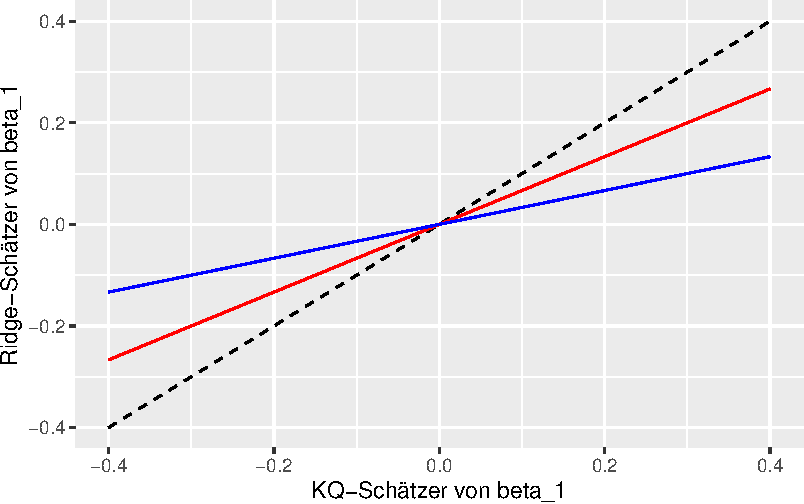
\includegraphics{RegReg_files/figure-pdf/fig-ridgeortho-1.pdf}

}

\caption{\label{fig-ridgeortho}Shrinkage des OLS-Schätzers bei Ridge
Regression}

\end{figure}%

Abbildung~\ref{fig-ridgeortho} zeigt, dass der Ridge-Schätzer eine
lineare Transformation des KQ-Schätzers (gestrichelte Linie) ist.
Größere Werte des Regularisierungsparameters \(\lambda\) führen zu
stärkerer Shrinkage des Koeffizientenschätzers in Richtung 0. Die
\(\ell_2\)-Norm führt zu proportional zum Absolutwert des KQ-Schätzers
verlaufender Shrinkage: Größere Koeffizienten werden stärker bestraft
als kleine Koeffizienten.

Die Eigenschaft
\[\mathrm{E}\left(\widehat{\boldsymbol{\beta}}^{\mathrm{R}}_{\lambda,\,j}\right) = (1+\lambda)^{-1} \cdot \beta_j\]
zeigt, dass \(\widehat{\boldsymbol{\beta}}^{\mathrm{R}}_{\lambda,\,j}\)
(für fixes \(\lambda>0\)) nicht erwartungstreu für \(\beta_j\) ist.
Weiterhin ist \begin{align*}
  \mathrm{Var}\left(\widehat{\beta}^{\mathrm{R}}_{\lambda,\,j}\right) =&\, 
  \mathrm{Var}\left(\widehat{\beta}_j\right) \cdot \left(\frac{\lambda}{1+\lambda^2}\right)\\
    =&\, \sigma^2\cdot \left(\frac{\lambda}{1+\lambda^2}\right),
\end{align*} wobei \(\sigma^2\) die Varianz des Regressionsfehlers \(u\)
ist. Wegen \(\lambda<(1+\lambda)^2\) für \(\lambda>0\) gilt
\[\mathrm{Var}\left(\widehat{\beta}^{\mathrm{R}}_{\lambda,\,j}\right)<\mathrm{Var}\left(\widehat{\beta}_j\right).\]
Der Ridge-Schätzer hat also eine kleinere Varianz als der KQ-Schätzer.
Diese Eigenschaften können auch für korrelierte Regressoren gezeigt
werden.

\subsection{\texorpdfstring{Ridge Regression mit
\texttt{glmnet}}{Ridge Regression mit glmnet}}\label{ridge-regression-mit-glmnet}

Wir zeigen nun anhand simulierter Daten, wie der Ridge-Lösungspfad mit
dem R-Paket \texttt{glmnet} berechnet werden kann. Wir erzeugen zunächst
Daten gemäß der Vorschrift \begin{align}
  \begin{split}
  Y_i =&\, \boldsymbol{X}_i' \boldsymbol{\beta} + u_i,\\
  \\
  \beta_j =&\,  \frac{5}{j^2}, \qquad\qquad\ j=1,\dots,5,\\ 
  \beta_j =&\, -\frac{5}{(j-5)^2}, \quad j=6,\dots,10,\\
  \\
  \boldsymbol{X}_i \sim&\, N(\boldsymbol{0}, \boldsymbol{\Sigma}), \quad u_i \overset{u.i.v.}{\sim} N(0, 1), \quad i = 1,\dots,25.
  \end{split} \label{eq:ridgedgp1}
\end{align} Hierbei wird \(\boldsymbol{\Sigma}\) so definiert, dass
jeder Regressor \(N(0,1)\)-verteilt ist und eine Korrelation von \(0.8\)
mit allen anderen Regressoren aufweist. Mit der Vorschrift für die
\(\beta_j\) stellen wir sicher, dass es wenige Variablen gibt, die \(Y\)
stark beeinflussen, da der Absolutbetrag der Koeffizienten in \(j\)
abnimmt.\footnote{Für bessere Interpretierbarkeit der Grafischen
  Auswertung, wählen wir positive und negative Koeffizienten mit
  gleichem Bertag.}

\begin{Shaded}
\begin{Highlighting}[]
\FunctionTok{library}\NormalTok{(gendata)}
\FunctionTok{set.seed}\NormalTok{(}\DecValTok{1234}\NormalTok{)}

\CommentTok{\# Parameter definieren}
\NormalTok{N }\OtherTok{\textless{}{-}} \DecValTok{80}
\NormalTok{k }\OtherTok{\textless{}{-}} \DecValTok{10}

\NormalTok{coefs }\OtherTok{\textless{}{-}} \DecValTok{5}\SpecialCharTok{/}\NormalTok{(}\DecValTok{1}\SpecialCharTok{:}\NormalTok{(k}\SpecialCharTok{/}\DecValTok{2}\NormalTok{))}\SpecialCharTok{\^{}}\DecValTok{2}
\NormalTok{beta }\OtherTok{\textless{}{-}} \FunctionTok{c}\NormalTok{(coefs, }\SpecialCharTok{{-}}\NormalTok{coefs)}

\CommentTok{\# Beobachtungen simulieren}
\NormalTok{X }\OtherTok{\textless{}{-}} \FunctionTok{as.matrix}\NormalTok{(}
  \FunctionTok{genmvnorm}\NormalTok{(}
    \AttributeTok{k =}\NormalTok{ k, }
    \AttributeTok{cor =} \FunctionTok{rep}\NormalTok{(.}\DecValTok{8}\NormalTok{, (k}\SpecialCharTok{\^{}}\DecValTok{2}\SpecialCharTok{{-}}\NormalTok{k)}\SpecialCharTok{/}\DecValTok{2}\NormalTok{), }
    \AttributeTok{n =}\NormalTok{ N)}
\NormalTok{  )}
\NormalTok{Y }\OtherTok{\textless{}{-}}\NormalTok{ X }\SpecialCharTok{\%*\%}\NormalTok{ beta }\SpecialCharTok{+} \FunctionTok{rnorm}\NormalTok{(N)}
\end{Highlighting}
\end{Shaded}

Wir schätzen nun ein Modell mit allen 10 Regressoren mit
\texttt{glmnet}. Beachte, dass für den Ridge-Strafterm
\texttt{alpha\ =\ 0} gesetzt werden muss.\footnote{\texttt{alpha} ist
  ein Mischparameter im Algorithmus für
  \href{https://en.wikipedia.org/wiki/Elastic_net_regularization}{elastic
  net}, siehe \texttt{?glmnet}.}

\begin{Shaded}
\begin{Highlighting}[]
\FunctionTok{library}\NormalTok{(glmnet)}

\CommentTok{\# Ridge{-}Regression anpassen}
\NormalTok{ridge\_fit }\OtherTok{\textless{}{-}} \FunctionTok{glmnet}\NormalTok{(}
  \AttributeTok{x =}\NormalTok{ X, }
  \AttributeTok{y =}\NormalTok{ Y, }
  \AttributeTok{alpha =} \DecValTok{0} \CommentTok{\# für Ridge{-}Strafterm}
\NormalTok{)}
\end{Highlighting}
\end{Shaded}

Der Lösungspfad der Ridge-Schätzung kann nach Transformation der
geschätzen Koeffizienten und der zugehörigen \(\lambda\)-Werte in ein
langes Format überführt und komfortabel mit \texttt{ggplot2} dargestellt
werden.

\begin{Shaded}
\begin{Highlighting}[]
\CommentTok{\# Lambda{-}Sequenz auslesen}
\NormalTok{lambdas }\OtherTok{\textless{}{-}}\NormalTok{ ridge\_fit}\SpecialCharTok{$}\NormalTok{lambda}

\CommentTok{\# Ridge{-}Schätzung für Lambdas im langen Format }
\FunctionTok{as.matrix}\NormalTok{(ridge\_fit}\SpecialCharTok{$}\NormalTok{beta) }\SpecialCharTok{\%\textgreater{}\%} 
  \FunctionTok{as\_tibble}\NormalTok{() }\SpecialCharTok{\%\textgreater{}\%} 
  \FunctionTok{rownames\_to\_column}\NormalTok{(}\StringTok{"Variable"}\NormalTok{) }\SpecialCharTok{\%\textgreater{}\%}
  \FunctionTok{pivot\_longer}\NormalTok{(}\SpecialCharTok{{-}}\NormalTok{Variable) }\SpecialCharTok{\%\textgreater{}\%} 
  \FunctionTok{group\_by}\NormalTok{(Variable) }\SpecialCharTok{\%\textgreater{}\%} 
  \FunctionTok{mutate}\NormalTok{(}\AttributeTok{lambda =}\NormalTok{ lambdas) }\SpecialCharTok{\%\textgreater{}\%}
  
  \CommentTok{\# Grafik mit ggplot erzeugen}
  \FunctionTok{ggplot}\NormalTok{(}
    \AttributeTok{mapping =} \FunctionTok{aes}\NormalTok{(}
      \AttributeTok{x =}\NormalTok{ lambda, }
      \AttributeTok{y =}\NormalTok{ value, }
      \AttributeTok{col =}\NormalTok{ Variable}
\NormalTok{    )}
\NormalTok{  ) }\SpecialCharTok{+} 
  \FunctionTok{geom\_line}\NormalTok{() }\SpecialCharTok{+}
  \FunctionTok{ylab}\NormalTok{(}\StringTok{"gesch. Koeffizienten"}\NormalTok{) }\SpecialCharTok{+}
  \FunctionTok{scale\_x\_log10}\NormalTok{(}\StringTok{"log\_10(lambda)"}\NormalTok{)}
\end{Highlighting}
\end{Shaded}

\begin{figure}[t]

\centering{

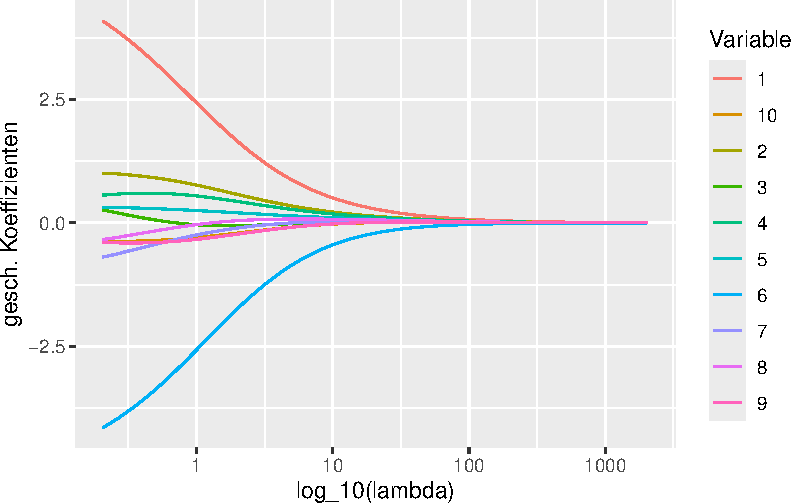
\includegraphics{RegReg_files/figure-pdf/fig-ridgesolpath-1.pdf}

}

\caption{\label{fig-ridgesolpath}Lösungspfad für Ridge-Schätzung}

\end{figure}%

Abbildung~\ref{fig-ridgesolpath} zeigt den nicht-linearen Verlauf der
Shrinkage auf den geschätzten Modellkoeffizienten. Die Koeffizienten
werden mit zunehmendem \(\lambda\) von der KQ-Lösung ausgehend (linkes
Ende der Skala) in Richtung 0 gezwungen.

Über die Funktion \texttt{cv.glmnet()} kann ein optimales \(\lambda\)
mit Cross Validation (CV) ermittelt werden. Ähnlich wie bei
\texttt{glmnet()} wird für die Validierung automatisch eine
\(\lambda\)-Sequenz erzeugt. Wir nutzen \texttt{autoplot()} aus dem
R-Paket \texttt{ggfortify} für die Visualisierung der Ergebnisse mit
\texttt{ggplot2}.

\begin{Shaded}
\begin{Highlighting}[]
\FunctionTok{library}\NormalTok{(ggfortify)}

\CommentTok{\# Cross{-}validierte Bestimmung von lambda}
\NormalTok{ridge\_cvfit }\OtherTok{\textless{}{-}} \FunctionTok{cv.glmnet}\NormalTok{(}
  \AttributeTok{y =}\NormalTok{ Y, }
  \AttributeTok{x =}\NormalTok{ X, }
  \AttributeTok{intercept =}\NormalTok{ F,}
  \AttributeTok{alpha =} \DecValTok{0}
\NormalTok{) }

\CommentTok{\# Ergebnisse plotten}
\NormalTok{ridge\_cvfit }\SpecialCharTok{\%\textgreater{}\%} 
  \FunctionTok{autoplot}\NormalTok{(}\AttributeTok{label.n =} \DecValTok{0}\NormalTok{)}
\end{Highlighting}
\end{Shaded}

\begin{figure}[t]

\centering{

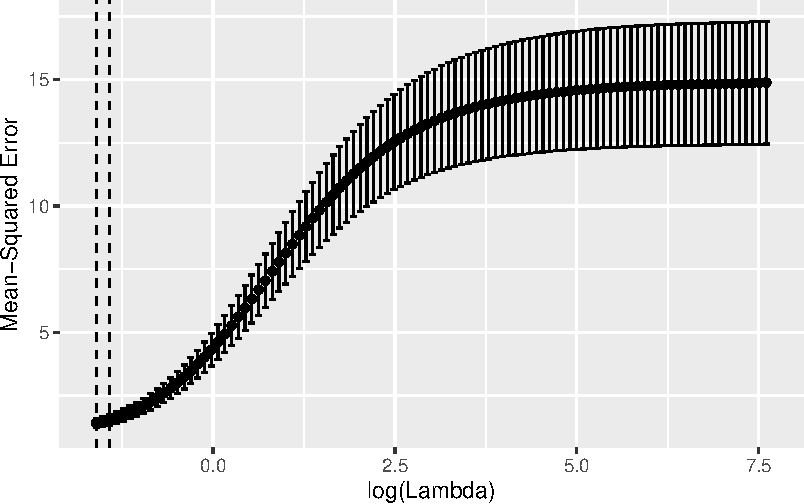
\includegraphics{RegReg_files/figure-pdf/fig-ridgecvplot-1.pdf}

}

\caption{\label{fig-ridgecvplot}Lösungspfad für Ridge-Schätzung}

\end{figure}%

Abbildung~\ref{fig-ridgecvplot} zeigt \texttt{ridge\_cvfit\$lambda.min},
das optimale \(\lambda\) mit dem geringsten CV Mean-Squarred-Error
(linke gestrichelte Linie) und \texttt{ridge\_cvfit\$lambda.1se}, das
größte \(\lambda\), welches innerhalb einer Standardabweichung entfernt
ist (rechte gestrichelte Linie).\footnote{Die Wahl von
  \texttt{lambda.1se} ist eine Heuristik, welche die Schätzunsicherheit
  berücksichtigt und zu einem ``sparsameren'' Modell tendiert.} Wir
berechnen die Schätzung für \texttt{lambda.min}.

\begin{Shaded}
\begin{Highlighting}[]
\NormalTok{(}
\NormalTok{  ridge\_coefs }\OtherTok{\textless{}{-}} \FunctionTok{coef}\NormalTok{(}
    \AttributeTok{object =}\NormalTok{ ridge\_cvfit, }
    \AttributeTok{s =}\NormalTok{ ridge\_cvfit}\SpecialCharTok{$}\NormalTok{lambda.min}
\NormalTok{  )}
\NormalTok{)}
\end{Highlighting}
\end{Shaded}

\begin{verbatim}
11 x 1 sparse Matrix of class "dgCMatrix"
                    s1
(Intercept)  .        
X1           4.1302194
X2           1.0245661
X3           0.3139297
X4           0.5697498
X5           0.2928664
X6          -4.1693524
X7          -0.7509305
X8          -0.3844761
X9          -0.3841997
X10         -0.4078514
\end{verbatim}

Wir schätzen das Modell nun mit KQ und vergleichen die Koeffizienten mit
der Ridge-Schätzung.

\begin{Shaded}
\begin{Highlighting}[]
\CommentTok{\# KQ{-}Schätzung durchführen}
\NormalTok{KQ\_fit }\OtherTok{\textless{}{-}} \FunctionTok{lm}\NormalTok{(Y }\SpecialCharTok{\textasciitilde{}}\NormalTok{ X }\SpecialCharTok{{-}} \DecValTok{1}\NormalTok{)}

\CommentTok{\# Koeffizienten auslesen und transformieren:}
\FunctionTok{tibble}\NormalTok{(}
  \AttributeTok{Ridge =} \FunctionTok{as.matrix}\NormalTok{(ridge\_coefs)[}\DecValTok{2}\SpecialCharTok{:}\DecValTok{11}\NormalTok{, ],}
  \AttributeTok{KQ =}\NormalTok{ KQ\_fit}\SpecialCharTok{$}\NormalTok{coefficients}
\NormalTok{) }\SpecialCharTok{\%\textgreater{}\%} 
  \FunctionTok{mutate}\NormalTok{(}\AttributeTok{j =} \FunctionTok{factor}\NormalTok{(}\DecValTok{1}\SpecialCharTok{:}\DecValTok{10}\NormalTok{)) }\SpecialCharTok{\%\textgreater{}\%}
  \FunctionTok{pivot\_longer}\NormalTok{(}
    \AttributeTok{cols =}\NormalTok{ Ridge}\SpecialCharTok{:}\NormalTok{KQ, }
    \AttributeTok{names\_to =} \StringTok{"Methode"}\NormalTok{, }
    \AttributeTok{values\_to =} \StringTok{"Koeffizient"}
\NormalTok{  ) }\SpecialCharTok{\%\textgreater{}\%}

\CommentTok{\# Bar{-}Plot für Koeffizientenvergleich erzeugen  }
  \FunctionTok{ggplot}\NormalTok{(}
    \AttributeTok{mapping =} \FunctionTok{aes}\NormalTok{(}
      \AttributeTok{x =}\NormalTok{ j, }
      \AttributeTok{y =}\NormalTok{ Koeffizient, }
      \AttributeTok{fill =}\NormalTok{ Methode}
\NormalTok{    )}
\NormalTok{  ) }\SpecialCharTok{+}
  \FunctionTok{geom\_bar}\NormalTok{(}
    \AttributeTok{position =} \StringTok{"dodge"}\NormalTok{, }
    \AttributeTok{stat =} \StringTok{"identity"}\NormalTok{, }
    \AttributeTok{width =}\NormalTok{ .}\DecValTok{5}
\NormalTok{  )}
\end{Highlighting}
\end{Shaded}

\begin{figure}[t]

\centering{

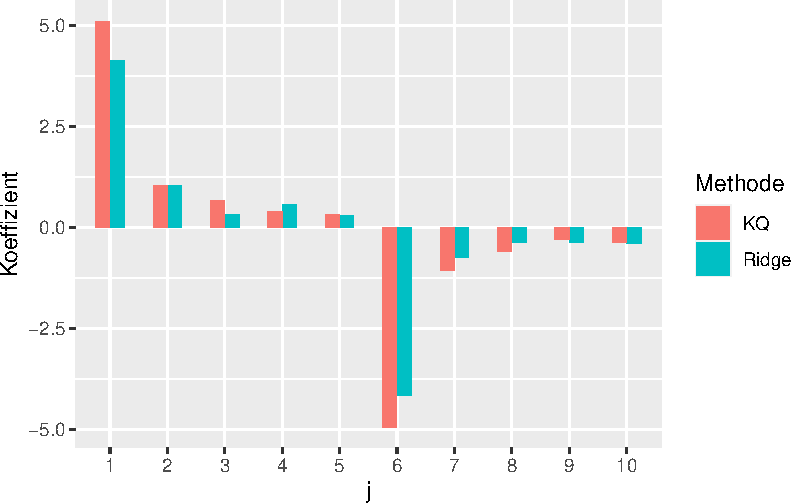
\includegraphics{RegReg_files/figure-pdf/fig-KoefRidgeVsKQ-1.pdf}

}

\caption{\label{fig-KoefRidgeVsKQ}Koeffizientenvergleich: Ridge vs.~KQ}

\end{figure}%

Der Vergleich anhand von Abbildung~\ref{fig-KoefRidgeVsKQ} zeigt
deutlich, dass Ridge Regression im Vergleich mit KQ zu absolut kleineren
Koeffizientenschätzungen tendiert. Inwiefern dies Konsequenzen für die
Prognosegüte der Schätzung hat, können wir Anhand eines Testdatensatzes
bestimmen. Hierzu vergleichen wir die mittleren Fehler (MSE) bei der
Prognose von \(Y\) für die Beobachtungen im Testdatensatz. Für die
Simulation des Testdatensatzes nutzen wir erneut die Vorschrift
\eqref{eq:ridgedgp1} um 80 neue Beobachtungen zu erzeugen.

\begin{Shaded}
\begin{Highlighting}[]
\CommentTok{\# Test{-}Datensatz erstellen}
\FunctionTok{set.seed}\NormalTok{(}\DecValTok{4321}\NormalTok{)}
\CommentTok{\# Regressoren}
\NormalTok{new\_X }\OtherTok{\textless{}{-}} \FunctionTok{as.matrix}\NormalTok{(}
  \FunctionTok{genmvnorm}\NormalTok{(}
    \AttributeTok{k =}\NormalTok{ k, }
    \AttributeTok{cor =} \FunctionTok{rep}\NormalTok{(.}\DecValTok{85}\NormalTok{, (k}\SpecialCharTok{\^{}}\DecValTok{2}\SpecialCharTok{{-}}\NormalTok{k)}\SpecialCharTok{/}\DecValTok{2}\NormalTok{), }
    \AttributeTok{n =}\NormalTok{ N}
\NormalTok{  )}
\NormalTok{)}
\CommentTok{\# Abh. Variable}
\NormalTok{new\_Y }\OtherTok{\textless{}{-}}\NormalTok{ new\_X }\SpecialCharTok{\%*\%}\NormalTok{ beta }\SpecialCharTok{+} \FunctionTok{rnorm}\NormalTok{(N)}
\end{Highlighting}
\end{Shaded}

Für beide Methoden können wir \texttt{predict()} für die Prognosen von
\(Y\) für den Testdatensatz (\texttt{new\_Y}) nutzen.

\begin{Shaded}
\begin{Highlighting}[]
\CommentTok{\# Ridge: Vorhersage von new\_Y für Test{-}Datensatz}
\NormalTok{Y\_predict\_ridge }\OtherTok{\textless{}{-}} \FunctionTok{predict}\NormalTok{(}
  \AttributeTok{object =}\NormalTok{ ridge\_cvfit, }
  \AttributeTok{newx =}\NormalTok{ new\_X, }
  \AttributeTok{s =}\NormalTok{ ridge\_cvfit}\SpecialCharTok{$}\NormalTok{lambda.min}
\NormalTok{)}

\CommentTok{\# Ridge: MSE für Test{-}Datensatz berechnen}
\FunctionTok{mean}\NormalTok{((Y\_predict\_ridge }\SpecialCharTok{{-}}\NormalTok{ new\_Y)}\SpecialCharTok{\^{}}\DecValTok{2}\NormalTok{)}
\end{Highlighting}
\end{Shaded}

\begin{verbatim}
[1] 1.288457
\end{verbatim}

Die Vorhersage für \texttt{lm()} benötigt dieselben Variablennamen wie
im angepassten Modell, s. \texttt{KQ\_fit\$coefficients}.

\begin{Shaded}
\begin{Highlighting}[]
\CommentTok{\# Test{-}Datensatz für predict.lm() formatieren}
\NormalTok{new\_X }\OtherTok{\textless{}{-}} \FunctionTok{as.data.frame}\NormalTok{(new\_X)}
\FunctionTok{colnames}\NormalTok{(new\_X) }\OtherTok{\textless{}{-}} \FunctionTok{paste0}\NormalTok{(}\StringTok{"X"}\NormalTok{, }\DecValTok{1}\SpecialCharTok{:}\NormalTok{k)}

\CommentTok{\# KQ: Vorhersage von new\_Y für Test{-}Datensatz}
\NormalTok{Y\_predict\_KQ }\OtherTok{\textless{}{-}} \FunctionTok{predict}\NormalTok{(}
  \AttributeTok{object =}\NormalTok{ KQ\_fit, }
  \AttributeTok{newdata =}\NormalTok{ new\_X}
\NormalTok{)}

\CommentTok{\# KQ: MSE für Test{-}Datensatz berechnen}
\FunctionTok{mean}\NormalTok{((Y\_predict\_KQ }\SpecialCharTok{{-}}\NormalTok{ new\_Y)}\SpecialCharTok{\^{}}\DecValTok{2}\NormalTok{)}
\end{Highlighting}
\end{Shaded}

\begin{verbatim}
[1] 29.33797
\end{verbatim}

Die Ergebnisse zeigen, dass der Ridge-Schätzer trotz seiner Verzerrung
einen deutlich geringeren mittleren Vorhersagefehler für die Testdaten
erzielt als der KQ-Schätzer. Diese Eigenschaft der
Koeffizientenschätzung kann die Prognosegüte von Ridge Regression
gegenüber der KQ-Regression verbessern.

\subsection{Beispiel: Vorhersage von Abschlussnoten in
Mathe}\label{beispiel-vorhersage-von-abschlussnoten-in-mathe}

Zur Illustration von Ridge Regression nutzen wir den Datensatz
\texttt{SP} aus Cortez und Silva (2008).\footnote{Wir verwenden eine
  Auszug aus dem Orignaldatensatz, der nebst ausführlicher
  Variablenbeschreibung
  \href{https://archive.ics.uci.edu/dataset/320/student+performance}{hier}
  verfügbar ist.} \texttt{SP} enhält Beobachtungen zu Leistungen von
insgesamt 100 Schülerinnen und Schülern im Fach Mathematik in der
Sekundarstufe an zwei portugiesischen Schulen. Neben der Abschlussnote
in Mathe (\texttt{G3}, Skala von 0 bis 20) beinhaltet \texttt{SP}
diverse demografische, soziale und schulbezogene Merkmale, die mithilfe
von Schulberichten und Fragebögen erhoben wurden. Ziel ist es, ein
Modell für die Prognose von \texttt{G3} anzupassen.

Wir lesen zunächst die Daten (im .csv-Format) ein.

\begin{Shaded}
\begin{Highlighting}[]
\CommentTok{\# Daten einlesen}
\NormalTok{SP }\OtherTok{\textless{}{-}} \FunctionTok{read\_csv}\NormalTok{(}\AttributeTok{file =} \StringTok{"datasets/SP.csv"}\NormalTok{)}
\end{Highlighting}
\end{Shaded}

Ein Überblick zeigt, dass der Großteil der Regressoren aus kategorialen
Variablen mit sozio-ökonomischen Informationen besteht.

\begin{Shaded}
\begin{Highlighting}[]
\CommentTok{\# Überblick}
\FunctionTok{glimpse}\NormalTok{(SP)}
\end{Highlighting}
\end{Shaded}

\begin{verbatim}
Rows: 100
Columns: 31
$ school     <chr> "GP", "GP", "GP", "MS", "GP", "GP", "GP", "GP", "GP", "GP",~
$ sex        <chr> "M", "M", "F", "F", "M", "F", "F", "F", "F", "F", "M", "M",~
$ age        <dbl> 17, 18, 19, 17, 16, 16, 19, 16, 16, 16, 18, 16, 15, 17, 17,~
$ address    <chr> "R", "R", "U", "U", "U", "U", "U", "U", "U", "R", "U", "U",~
$ famsize    <chr> "GT3", "GT3", "LE3", "GT3", "LE3", "GT3", "GT3", "GT3", "GT~
$ Pstatus    <chr> "T", "T", "T", "T", "A", "T", "T", "T", "A", "T", "T", "T",~
$ Medu       <dbl> 1, 4, 3, 2, 3, 2, 0, 2, 3, 4, 4, 2, 1, 2, 2, 3, 3, 4, 4, 2,~
$ Fedu       <dbl> 2, 3, 2, 2, 4, 3, 1, 1, 1, 4, 4, 2, 2, 3, 2, 3, 1, 3, 4, 2,~
$ Mjob       <chr> "at_home", "teacher", "services", "other", "services", "oth~
$ Fjob       <chr> "other", "services", "other", "at_home", "other", "other", ~
$ reason     <chr> "home", "course", "reputation", "home", "home", "reputation~
$ guardian   <chr> "mother", "mother", "other", "mother", "mother", "mother", ~
$ traveltime <dbl> 1, 1, 2, 1, 1, 1, 1, 1, 1, 1, 1, 2, 1, 1, 1, 2, 1, 1, 1, 1,~
$ studytime  <dbl> 2, 3, 2, 3, 2, 2, 2, 1, 2, 2, 1, 2, 2, 2, 1, 1, 2, 3, 1, 2,~
$ failures   <dbl> 0, 0, 1, 0, 0, 0, 3, 0, 3, 0, 0, 0, 0, 0, 0, 0, 0, 0, 0, 0,~
$ schoolsup  <chr> "no", "no", "no", "no", "yes", "yes", "no", "no", "no", "no~
$ famsup     <chr> "no", "no", "yes", "no", "yes", "yes", "yes", "no", "yes", ~
$ paid       <chr> "no", "no", "yes", "no", "no", "yes", "no", "no", "yes", "n~
$ activities <chr> "no", "no", "no", "yes", "yes", "yes", "no", "no", "no", "y~
$ nursery    <chr> "yes", "yes", "no", "yes", "yes", "yes", "no", "yes", "yes"~
$ higher     <chr> "yes", "yes", "yes", "yes", "yes", "yes", "no", "yes", "yes~
$ internet   <chr> "no", "yes", "yes", "no", "yes", "no", "no", "yes", "yes", ~
$ romantic   <chr> "no", "yes", "yes", "yes", "no", "no", "no", "yes", "no", "~
$ famrel     <dbl> 3, 5, 4, 3, 5, 4, 3, 4, 2, 2, 1, 5, 4, 5, 3, 5, 4, 4, 5, 5,~
$ freetime   <dbl> 1, 3, 2, 4, 3, 4, 4, 5, 3, 4, 4, 4, 3, 3, 4, 4, 5, 2, 3, 4,~
$ goout      <dbl> 3, 2, 2, 3, 3, 3, 2, 2, 3, 4, 2, 4, 2, 3, 4, 2, 4, 2, 3, 4,~
$ Dalc       <dbl> 1, 1, 1, 1, 1, 1, 1, 1, 2, 2, 2, 2, 1, 1, 1, 1, 2, 1, 1, 1,~
$ Walc       <dbl> 5, 2, 2, 1, 1, 3, 1, 1, 2, 3, 2, 4, 1, 3, 3, 1, 3, 2, 1, 1,~
$ health     <dbl> 3, 4, 1, 3, 5, 4, 5, 5, 4, 4, 1, 5, 5, 3, 5, 5, 1, 3, 5, 5,~
$ absences   <dbl> 4, 9, 22, 8, 4, 6, 2, 20, 5, 6, 5, 0, 2, 2, 12, 0, 17, 0, 4~
$ G3         <dbl> 10, 16, 11, 11, 11, 10, 9, 12, 7, 11, 16, 12, 9, 12, 12, 13~
\end{verbatim}

Um die Prognosegüte des Modells beurteilen zu können, partitionieren wir
\texttt{SP} zufällig in einen Test- sowie einen Trainingsdatensatz (mit
30 und 70 Beobachtungen), jeweils für die Regressoren und die abhängige
Variable.

\begin{Shaded}
\begin{Highlighting}[]
\CommentTok{\# ID für Beobachtungen im Testdatensatz zufällig erzeugen}
\FunctionTok{set.seed}\NormalTok{(}\DecValTok{1234}\NormalTok{)}
\NormalTok{ID }\OtherTok{\textless{}{-}} \FunctionTok{sample}\NormalTok{(}\DecValTok{1}\SpecialCharTok{:}\FunctionTok{nrow}\NormalTok{(SP), }\AttributeTok{size =} \DecValTok{30}\NormalTok{)}

\CommentTok{\# Regressoren aufteilen}
\NormalTok{SP\_test }\OtherTok{\textless{}{-}}\NormalTok{ SP[ID,]}
\NormalTok{SP\_train }\OtherTok{\textless{}{-}}\NormalTok{ SP[}\SpecialCharTok{{-}}\NormalTok{ID,]}

\CommentTok{\# Abh. Variable aufteilen}
\NormalTok{Y\_test }\OtherTok{\textless{}{-}}\NormalTok{ SP\_test}\SpecialCharTok{$}\NormalTok{G3}
\NormalTok{Y\_train }\OtherTok{\textless{}{-}}\NormalTok{ SP\_train}\SpecialCharTok{$}\NormalTok{G3}
\end{Highlighting}
\end{Shaded}

Als nächstes passen wir ein Ridge-Regressionsmodell für alle Regressoren
in \texttt{SP\_train} an und ermitteln ein optimales \(\lambda\) mit
Cross Validation. Beachte, dass \texttt{cv.glmnet} nicht für Regressoren
im \texttt{data.frame}/\texttt{tibble}-Format ausgelegt ist, sondern ein
\texttt{matrix}-Format erwartet. Wir transformieren \texttt{SP\_train}
daher mit \texttt{data.matrix()}.

\begin{Shaded}
\begin{Highlighting}[]
\CommentTok{\# Ridge{-}Regression und CV für Trainingsdaten}
\NormalTok{SP\_fit\_cv }\OtherTok{\textless{}{-}} \FunctionTok{cv.glmnet}\NormalTok{(}
  \AttributeTok{x =} \FunctionTok{data.matrix}\NormalTok{(SP\_train }\SpecialCharTok{\%\textgreater{}\%} \FunctionTok{select}\NormalTok{(}\SpecialCharTok{{-}}\NormalTok{G3)), }
  \AttributeTok{y =}\NormalTok{ Y\_train, }
  \AttributeTok{alpha =} \DecValTok{0}
\NormalTok{)}

\CommentTok{\# CV{-}Ergebnisse für lambda visualisieren}
\NormalTok{SP\_fit\_cv }\SpecialCharTok{\%\textgreater{}\%} 
  \FunctionTok{autoplot}\NormalTok{(}\AttributeTok{label.n =} \DecValTok{0}\NormalTok{)}
\end{Highlighting}
\end{Shaded}

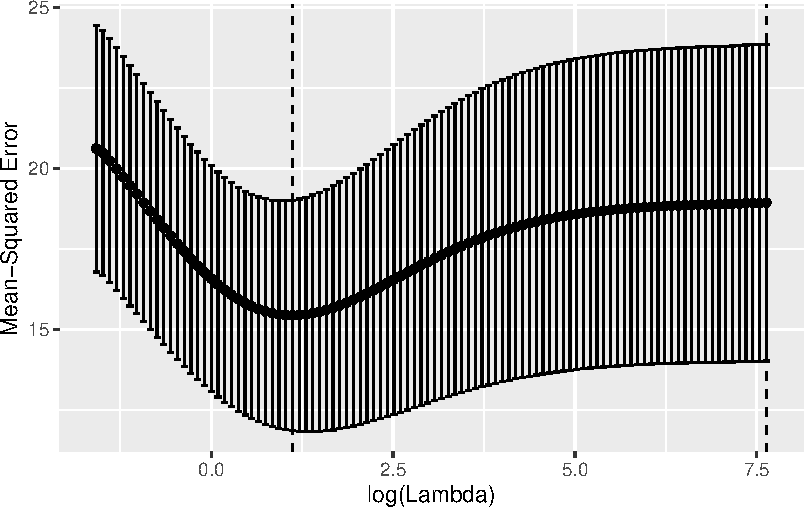
\includegraphics{RegReg_files/figure-pdf/unnamed-chunk-16-1.pdf}

Wie für das Beispiel mit simulierten Daten erhalten wir mit
\texttt{predict()} Vorhersagen für die erzielte Punktzahl. Beachte, dass
wir den MSE nicht für die Trainingsdaten \texttt{SP\_train}, sondern für
die Testdaten \texttt{SP\_test} berechnen.

\begin{Shaded}
\begin{Highlighting}[]
\CommentTok{\# Prognose von G3 anhand des Ridge{-}Modells}
\NormalTok{Y\_predict\_ridge }\OtherTok{\textless{}{-}} \FunctionTok{predict}\NormalTok{(}
  \AttributeTok{object =}\NormalTok{ SP\_fit\_cv, }
  \AttributeTok{newx =} \FunctionTok{data.matrix}\NormalTok{(}
\NormalTok{    SP\_test }\SpecialCharTok{\%\textgreater{}\%} 
      \FunctionTok{select}\NormalTok{(}\SpecialCharTok{{-}}\NormalTok{G3)}
\NormalTok{    ), }
  \AttributeTok{s =}\NormalTok{ SP\_fit\_cv}\SpecialCharTok{$}\NormalTok{lambda.min}
\NormalTok{)}

\CommentTok{\# MSE für Testdaten berechnen}
\FunctionTok{mean}\NormalTok{((Y\_predict\_ridge }\SpecialCharTok{{-}}\NormalTok{ Y\_test)}\SpecialCharTok{\^{}}\DecValTok{2}\NormalTok{)}
\end{Highlighting}
\end{Shaded}

\begin{verbatim}
[1] 21.13249
\end{verbatim}

Auch in diesem empirischen Beispiel zeigt ein Vergleich der MSEs, dass
Ridge Regression dem KQ-Schätzer hinsichtlich der Vorhersagegüte
überlegen ist.

\begin{Shaded}
\begin{Highlighting}[]
\CommentTok{\# Modell mit KQ schätzen}
\NormalTok{SP\_fit\_KQ }\OtherTok{\textless{}{-}} \FunctionTok{lm}\NormalTok{(G3 }\SpecialCharTok{\textasciitilde{}}\NormalTok{ ., SP\_train)}

\CommentTok{\# Prognose}
\NormalTok{Y\_predict\_KQ }\OtherTok{\textless{}{-}} \FunctionTok{predict}\NormalTok{(}
  \AttributeTok{object =}\NormalTok{ SP\_fit\_KQ, }
  \AttributeTok{newdata =}\NormalTok{ SP\_test }\SpecialCharTok{\%\textgreater{}\%} 
    \FunctionTok{select}\NormalTok{(}\SpecialCharTok{{-}}\NormalTok{G3)}
\NormalTok{)}

\CommentTok{\# Testset{-}MSE berechnen}
\FunctionTok{mean}\NormalTok{((Y\_predict\_KQ }\SpecialCharTok{{-}}\NormalTok{ Y\_test)}\SpecialCharTok{\^{}}\DecValTok{2}\NormalTok{)}
\end{Highlighting}
\end{Shaded}

\begin{verbatim}
[1] 29.76893
\end{verbatim}

Der MSE für Ridge ist mit \(21.13\) deutlich kleiner als \(29.77\), der
MSE für KQ.

Für die Interpretation der Ridge-Schätzung erweitern den Code für die
\texttt{ggplot2}-Grafik der Koeffizienten-Pfade um eine vertikale Linie
des mit CV ermittelten \(\lambda\) und fügen mit dem Paket
\texttt{ggrepel} Labels für die Pfade der größten Koeffizienten hinzu.

\begin{Shaded}
\begin{Highlighting}[]
\FunctionTok{library}\NormalTok{(ggrepel)}

\CommentTok{\# Lambda{-}Sequenz auslesen}
\NormalTok{lambdas }\OtherTok{\textless{}{-}}\NormalTok{ SP\_fit\_cv}\SpecialCharTok{$}\NormalTok{lambda}

\CommentTok{\# Ridge{-}Schätzung für Lambdas im langen Format }
\NormalTok{df }\OtherTok{\textless{}{-}} \FunctionTok{as.matrix}\NormalTok{(SP\_fit\_cv}\SpecialCharTok{$}\NormalTok{glmnet.fit}\SpecialCharTok{$}\NormalTok{beta) }\SpecialCharTok{\%\textgreater{}\%} 
  \FunctionTok{as\_tibble}\NormalTok{() }\SpecialCharTok{\%\textgreater{}\%} 
  \FunctionTok{mutate}\NormalTok{(}
    \AttributeTok{Variable =} \FunctionTok{rownames}\NormalTok{(SP\_fit\_cv}\SpecialCharTok{$}\NormalTok{glmnet.fit}\SpecialCharTok{$}\NormalTok{beta)}
\NormalTok{  ) }\SpecialCharTok{\%\textgreater{}\%}
  \FunctionTok{pivot\_longer}\NormalTok{(}\SpecialCharTok{{-}}\NormalTok{Variable) }\SpecialCharTok{\%\textgreater{}\%} 
  \FunctionTok{group\_by}\NormalTok{(Variable) }\SpecialCharTok{\%\textgreater{}\%} 
  \FunctionTok{mutate}\NormalTok{(}\AttributeTok{lambda =}\NormalTok{ lambdas) }

\CommentTok{\# Grafik mit ggplot erzeugen}
\NormalTok{df }\SpecialCharTok{\%\textgreater{}\%}
  \FunctionTok{ggplot}\NormalTok{(}
    \AttributeTok{mapping =} \FunctionTok{aes}\NormalTok{(}
      \AttributeTok{x =}\NormalTok{ lambda, }
      \AttributeTok{y =}\NormalTok{ value, }
      \AttributeTok{col =}\NormalTok{ Variable}
\NormalTok{    )}
\NormalTok{  ) }\SpecialCharTok{+} 
  \FunctionTok{geom\_line}\NormalTok{() }\SpecialCharTok{+}
  \FunctionTok{geom\_label\_repel}\NormalTok{(}
    \AttributeTok{data =}\NormalTok{ df }\SpecialCharTok{\%\textgreater{}\%} 
      \FunctionTok{filter}\NormalTok{(lambda }\SpecialCharTok{==} \FunctionTok{min}\NormalTok{(lambdas)),}
    \AttributeTok{mapping =} \FunctionTok{aes}\NormalTok{(}\AttributeTok{label =}\NormalTok{ Variable), }
    \AttributeTok{seed =} \DecValTok{1234}\NormalTok{,}
    \AttributeTok{size =} \DecValTok{5}\NormalTok{, }
    \AttributeTok{max.overlaps =} \DecValTok{8}\NormalTok{, }
    \AttributeTok{nudge\_x =} \SpecialCharTok{{-}}\NormalTok{.}\DecValTok{5}\NormalTok{) }\SpecialCharTok{+}
  \FunctionTok{ylab}\NormalTok{(}\StringTok{"gesch. Koeffizienten"}\NormalTok{) }\SpecialCharTok{+}
  \FunctionTok{scale\_x\_log10}\NormalTok{(}\StringTok{"log\_10(lambda)"}\NormalTok{) }\SpecialCharTok{+}
  \FunctionTok{geom\_vline}\NormalTok{(}
    \AttributeTok{xintercept =}\NormalTok{ SP\_fit\_cv}\SpecialCharTok{$}\NormalTok{lambda.min, }
    \AttributeTok{col =} \StringTok{"red"}\NormalTok{, }
    \AttributeTok{lty =} \DecValTok{2}
\NormalTok{  ) }\SpecialCharTok{+}
  \FunctionTok{theme}\NormalTok{(}\AttributeTok{legend.position =} \StringTok{"none"}\NormalTok{)}
\end{Highlighting}
\end{Shaded}

\begin{figure}[t]

\centering{

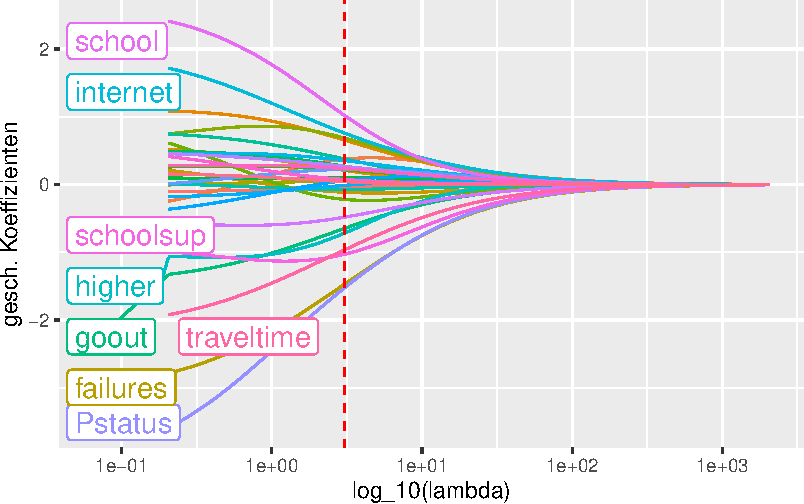
\includegraphics{RegReg_files/figure-pdf/fig-ridgAppPlot-1.pdf}

}

\caption{\label{fig-ridgAppPlot}Lösungspfad für Ridge-Schätzung}

\end{figure}%

Abbildung~\ref{fig-ridgAppPlot} gibt Hinweise darauf, dass neben der
Schulzugehörigkeit und Indikatoren für schulische Leistung (bspw.
\texttt{failures}) sozio-ökonomische Prädiktoren wie \texttt{internet}
(Internetzugang zuhause), \texttt{Pstatus} (Zusammenleben der Eltern)
und \texttt{address}/\texttt{traveltime} (sozialer Status) relevante
Variablen zu sein scheinen.

Das optimale \(\lambda_\mathrm{cv} \approx 0.21\) (gestrichelte rote
Linie in Abbildung~\ref{fig-ridgAppPlot}) führt zu deutlicher Shrinkage,
was eine mögliche Erklärung für den besseren Testset-MSE von Ridge
Regression ist: Die Koeffizienten von Variablen mit wenig
Erklärungskraft werden durch die Regularisierung in Richtung 0 gezwungen
und reduzieren so die Varianz der Vorhersage gegenüber der
(idealerweise) unverzerrten KQ-Schätzung.

\begin{tcolorbox}[enhanced jigsaw, bottomtitle=1mm, colbacktitle=quarto-callout-note-color!10!white, coltitle=black, arc=.35mm, title=\textcolor{quarto-callout-note-color}{\faInfo}\hspace{0.5em}{Key Facts zu Ridge Regression}, titlerule=0mm, opacityback=0, breakable, bottomrule=.15mm, toprule=.15mm, opacitybacktitle=0.6, colframe=quarto-callout-note-color-frame, toptitle=1mm, rightrule=.15mm, leftrule=.75mm, left=2mm, colback=white]

\begin{itemize}
\item
  Ridge-Regression regularisiert den KQ-Schätzer mit der \(\ell_2\)-Norm
  der Koeffizienten. Diese Form von Regularisierung ist eine Alternative
  für KQ in Anwendungen mit mehr Regressoren als Beobachtugen
  (\(k\geq n\)) und/oder wenn KQ aufgrund starker Kollinearität eine
  hohe Varianz aufweist.
\item
  Der Ridge-Schätzer
  \(\widehat{\boldsymbol{\beta}}^{\mathrm{R}}_\lambda\) ist \emph{nicht}
  erwartungstreu. Die geschätzten Koeffizienten sind auch für
  \(n\to\infty\) verzerrt.
\item
  Aufgrund der verzerrten Schätzung ist statistische Inferenz für
  Koeffizienten mit
  \(\widehat{\boldsymbol{\beta}}^{\mathrm{R}}_\lambda\) problematisch.
  Anstatt für strukturelle Modelle oder die Schätzung kausaler Effekte
  wird Ridge Regression in der Praxis daher überwiegend für Prognosen
  verwendet.
\item
  Die Wahl von \(\lambda\) impliziert einen Tradeoff zwischen Verzerrung
  und Varianz: Große \(\lambda\) schrumpfen die Koeffizientenschätzer
  Richtung 0 (mehr Verzerrung), führen aber zu einer kleineren Varianz
  der Schätzung. Entsprechend können Vorhersagen mit mehr Verzerrung
  aber weniger Varianz als mit KQ getroffen werden.
\item
  Ridge Regression kann in R mit dem Paket \texttt{glmnet} berechnet
  werden.
\end{itemize}

\end{tcolorbox}

\section{Lasso Regression}\label{lasso-regression}

Least Absolute Shrinkage and Selection Operator (Lasso) ist ein von
Tibshirani (1996) vorgeschlagener Schätzer, der die Verlustfunktion des
KQ-Schätzers um einen Strafterm für die Summe der (absoluten) Größe der
Koeffizienten \(\boldsymbol\beta = (\beta_1, \dots,\beta_k)'\)
erweitert. Die Verlustfunktion des Lasso-Schätzers von
\(\boldsymbol{\beta}\) lautet \begin{align}
\mathrm{RSS}(\boldsymbol{\beta},p=1,\lambda) = \mathrm{RSS}(\boldsymbol{\beta}) + \lambda \lVert\boldsymbol{\beta}\rVert_1.\label{eq:lassoloss}
\end{align} Für den Strafterm wird also die \(\ell_1\)-norm \[
\lVert\boldsymbol{\beta}\rVert_1 = \sum_{j=1}^k \lvert\beta_j \rvert
\] verwendet. Der Lasso-Schätzer
\(\widehat{\boldsymbol{\beta}}^{\mathrm{L}}_\lambda\) für
\(\boldsymbol{\beta}\) minimiert \eqref{eq:lassoloss}, \begin{align}
\boldsymbol{\beta}^{\mathrm{L}}_\lambda = \arg\min_{\boldsymbol{\beta}} \ \mathrm{RSS}(\boldsymbol{\beta},p=1,\lambda).
\end{align} Entsprechend erhalten wir in Abhängigkeit von \(\lambda\)
ein Kontinuum an Lösungen \begin{align}
  \left\{\widehat{\boldsymbol{\beta}}^{\mathrm{L}}_\lambda\right\}_{\lambda=0}^{\lambda=\infty},\label{eq:LassoPath}
\end{align} der sogenannte \emph{Lasso-Pfad}.

Das Optimierungsproblem \eqref{eq:lassoloss} hat die äquivalente
Darstellung \begin{align}
  \begin{split}
    \widehat{\boldsymbol{\beta}}^{\mathrm{L}}_\lambda =&\, \arg\min_{\boldsymbol{\beta}} \mathrm{RSS}(\boldsymbol{\beta}) + \lambda\left(\lVert\boldsymbol{\beta}\rVert_1 - t\right)\\
    =&\, \arg\min_{\lVert\boldsymbol{\beta}\rVert_1\leq t} \mathrm{RSS}(\boldsymbol{\beta}), 
  \end{split}\label{eq:lassolagrange}
\end{align} welche über den
\href{https://de.wikipedia.org/wiki/Lagrange-Multiplikator\#Beispiel_mit_Anwendungsbezug}{Lagrange-Ansatz}
unter der Nebenbedingung \(\lVert\boldsymbol{\beta}\rVert_1 \leq t\)
gelöst werden kann.

Ähnlich wie der KQ-Schätzer ist der Lasso-Schätzer
\(\widehat{\boldsymbol{\beta}}^{\mathrm{L}}_\lambda\) durch Bedingungen
1. Ordnung bestimmt. Diese Bedingungen lassen sich komfortabel in
Matrix-Schreibweise darstellen als \begin{align}
  -2\boldsymbol{X}_j'(\boldsymbol{Y} - \boldsymbol{X}\boldsymbol{\beta}) + \lambda\cdot\mathrm{sgn}(\beta_j) = 0, \quad j = 1,\dots,k.\label{eq:LassoFOC}
\end{align} Aus Gleichung \eqref{eq:LassoFOC} folgt, dass der
Lasso-Schätzer aufgrund des Strafterms im Allgemeinen nicht algebraisch
bestimmt werden kann.\footnote{Zur Bestimmung des Schätzers werden
  Algorithmen der nicht-linearen Optimierung genutzt.}

In Abhängigkeit von \(\lambda\) zwingt der Lasso-Schätzer die
KQ-Schätzung von \(\beta_j\) zu einem (absolut) kleineren Wert: Ähnlich
wie bei Ridge Regression bewirkt der \(\ell_1\)-Strafterm eine mit
\(\lambda\) zunehmende Schrumpfung der geschätzen Koeffizienten in
Richtung 0. Charakteristisch für die Lösung des Lasso-Schätzers ist,
dass \(\widehat{\boldsymbol{\beta}}^{\mathrm{L}}_j = 0\), wenn die
Bedingung \begin{align}
  \left\lvert\boldsymbol{X}_j'(\boldsymbol{Y} - \boldsymbol{X}\widehat{\boldsymbol{\beta}}^{\mathrm{L}}_\lambda)\right\rvert - \lambda/2 \leq 0 \label{eq:lassoselection}
\end{align} erfüllt ist. In Abhängigkeit von \(\lambda\) kann der
Lasso-Schätzer folglich geschätzte Regressionskoeffizienten nicht nur in
Richtung \(0\), sondern diese auch \emph{exakt} mit \(0\) schätzen und
damit \emph{Variablenselektion} betreiben. Aufgrund der mit \(\lambda\)
zunehmenden Shrinkage bis die Bedingung \eqref{eq:lassoselection}
erfüllt und der Koeffizient gleich \(0\) gesetzt wird, bezeichnet man
Lasso auch als einen \emph{Soft Thresholding Operator}. Im nächsten
Abschnitt betrachten wir die Eigenschaften von Lasso-Regularisierung
unter vereinfachten Annahmen bzgl. der Regressoren.

\subsection{Lasso ist Soft
Thresholding}\label{lasso-ist-soft-thresholding}

Wir betrachten nun eine mathematische Darstellung von Selektions- und
Shrinkage-Eigenschaft des Lasso-Schätzers in einem vereinfachten Modell.
Wenn die Regressoren \(\boldsymbol{X}\) orthonormal zueinander sind,
existiert eine analytische Lösung des Lasso-Schätzers, \begin{align}
  \widehat{\boldsymbol{\beta}}^{\mathrm{L}}_\lambda =
  \begin{cases}
    \widehat{\boldsymbol{\beta}}_j - \lambda/2 &, \ \ \widehat{\boldsymbol{\beta}}_j > \lambda/2\\
    0 &, \ \ \lvert\widehat{\boldsymbol{\beta}}_j\rvert\leq\lambda/2\\
    \widehat{\boldsymbol{\beta}}_j + \lambda/2 &, \ \ \widehat{\boldsymbol{\beta}}_j < \lambda/2
  \end{cases},\label{eq:lassoST}
\end{align} wobei \(\widehat{\boldsymbol{\beta}}_j\) der KQ-Schätzer von
\(\beta_j\) ist. Anhand von \eqref{eq:lassoST} können wir die
Selektionseigenschaft sowie die Schrumpfung der
KQ-Koeffizientenschätzung in Abhängigkeit der durch \(\lambda\)
regulierten \(\ell_1\)-Strafe erkennen. Für eine Visualisierung
implementieren wir \eqref{eq:lassoST} als R-Funktion
\texttt{lasso\_st()} und zeichnen die resultierenden
Koeffizientenschätzungen für die Parameterwerte
\(\lambda\in\{0, 0.2, 0.4\}\).

Wir definieren zunächst die Funktion \texttt{lasso\_st()}.

\begin{Shaded}
\begin{Highlighting}[]
\FunctionTok{library}\NormalTok{(tidyverse)}

\CommentTok{\# Funktion für Lasso soft{-}thresholding definieren}
\NormalTok{lasso\_st }\OtherTok{\textless{}{-}} \ControlFlowTok{function}\NormalTok{(KQ, lambda) \{}
  \FunctionTok{case\_when}\NormalTok{(}
\NormalTok{    KQ }\SpecialCharTok{\textgreater{}}\NormalTok{ lambda}\SpecialCharTok{/}\DecValTok{2}         \SpecialCharTok{\textasciitilde{}}\NormalTok{ KQ }\SpecialCharTok{{-}}\NormalTok{ lambda}\SpecialCharTok{/}\DecValTok{2}\NormalTok{,}
    \FunctionTok{abs}\NormalTok{(KQ) }\SpecialCharTok{\textless{}=}\NormalTok{ lambda}\SpecialCharTok{/}\DecValTok{2}   \SpecialCharTok{\textasciitilde{}} \DecValTok{0}\NormalTok{,}
\NormalTok{    KQ }\SpecialCharTok{\textless{}} \SpecialCharTok{{-}}\NormalTok{lambda}\SpecialCharTok{/}\DecValTok{2}        \SpecialCharTok{\textasciitilde{}}\NormalTok{ KQ }\SpecialCharTok{+}\NormalTok{ lambda}\SpecialCharTok{/}\DecValTok{2}\NormalTok{,}
\NormalTok{  )}
\NormalTok{\}}
\end{Highlighting}
\end{Shaded}

Im nächsten Schritt zeichnen wir \texttt{lasso\_st()} für eine Sequenz
von KQ-Schätzwerten gegeben \(\lambda\).

\begin{Shaded}
\begin{Highlighting}[]
\CommentTok{\# Sequenz von KQ{-}Schätzwerten für Illustration definieren}
\NormalTok{dat }\OtherTok{\textless{}{-}} \FunctionTok{tibble}\NormalTok{(}
  \AttributeTok{KQ =} \FunctionTok{seq}\NormalTok{(}\SpecialCharTok{{-}}\DecValTok{1}\NormalTok{, }\DecValTok{1}\NormalTok{, .}\DecValTok{01}\NormalTok{)}
\NormalTok{)}

\CommentTok{\# Lasso{-}Schätzer als Funktion des KQ{-}Schätzers plotten}
\FunctionTok{ggplot}\NormalTok{(dat) }\SpecialCharTok{+}
  \FunctionTok{geom\_function}\NormalTok{(}
    \AttributeTok{fun =}\NormalTok{ lasso\_st, }
    \AttributeTok{args =} \FunctionTok{list}\NormalTok{(}\AttributeTok{lambda =} \DecValTok{0}\NormalTok{), }
    \AttributeTok{lty =} \DecValTok{2}
\NormalTok{  ) }\SpecialCharTok{+} 
  \FunctionTok{geom\_function}\NormalTok{(}
    \AttributeTok{fun =}\NormalTok{ lasso\_st, }
    \AttributeTok{args =} \FunctionTok{list}\NormalTok{(}\AttributeTok{lambda =}\NormalTok{ .}\DecValTok{2}\NormalTok{),}
    \AttributeTok{col =} \StringTok{"red"}
\NormalTok{  ) }\SpecialCharTok{+} 
  \FunctionTok{geom\_function}\NormalTok{(}
    \AttributeTok{fun =}\NormalTok{ lasso\_st, }
    \AttributeTok{args =} \FunctionTok{list}\NormalTok{(}\AttributeTok{lambda =}\NormalTok{ .}\DecValTok{4}\NormalTok{), }
    \AttributeTok{col =} \StringTok{"blue"}
\NormalTok{  ) }\SpecialCharTok{+} 
  \FunctionTok{xlim}\NormalTok{(}\SpecialCharTok{{-}}\NormalTok{.}\DecValTok{4}\NormalTok{, .}\DecValTok{4}\NormalTok{) }\SpecialCharTok{+}
  \FunctionTok{xlab}\NormalTok{(}\StringTok{"KQ{-}Schätzer von beta\_1"}\NormalTok{) }\SpecialCharTok{+}
  \FunctionTok{ylab}\NormalTok{(}\StringTok{"Lasso{-}Schätzer von beta\_1"}\NormalTok{)}
\end{Highlighting}
\end{Shaded}

\begin{figure}[t]

\centering{

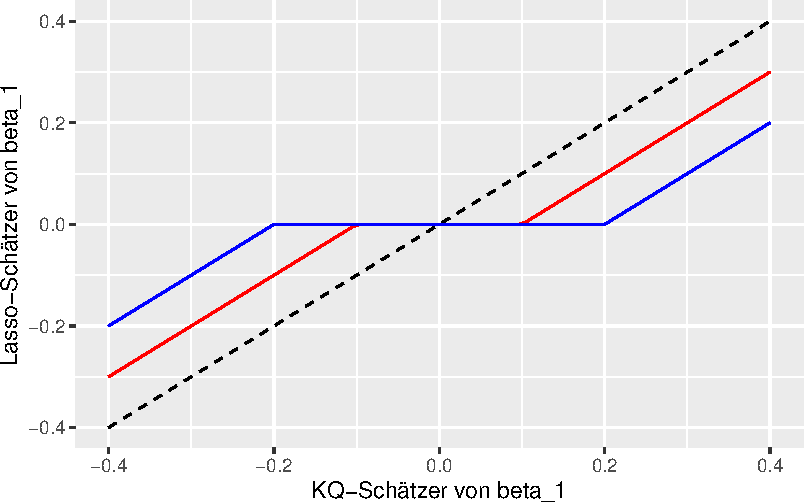
\includegraphics{RegReg_files/figure-pdf/fig-lassoST-1.pdf}

}

\caption{\label{fig-lassoST}Shrinkage und Selektion von
OLS-Koeffizienten mit Lasso}

\end{figure}%

Abbildung~\ref{fig-lassoST} zeigt, dass der \(\ell_1\)-Strafterm des
Lasso-Schätzers zu einem linearen Verlauf der auf den KQ-Schätzer
(gezeichnet für \(\lambda = 0\), gestrichelte Linie) applizierten
Shrinkage führt: Der Lasso-Schätzer ist eine abschnittsweise-lineare
Funktion des KQ-Schätzers in \(\lambda\): Je größer der Parameter
\(\lambda\), desto größer ist das Intervall von KQ-Schätzwerten
\([-\lambda/2,\lambda/2]\), wo der Lasso-Schätzer zu Variablenselektion
führt, d.h. hier den Koeffizienten \(\beta_j\) als \(0\) schätzt (rote
bzw. blaue Linie).

Anhand von Abbildung~\ref{fig-lassoST} kann abgeleitet werden, dass der
Lasso-Schätzer nicht invariant gegenüber der Skalierung der Regressoren
ist: Die Stärke der Regularisierung durch \(\lambda\) ist hängt von der
Magnitude des KQ-Schätzers ab. Daher müssen die Regressoren vor
Berechnung der Schätzung standardsiert werden. Üblich ist hierbei eine
Normierung auf einen Mittelwert von \(0\) und eine Varianz von \(1\).

Die nachstehende interaktive Grafik illustriert das
Lasso-Optimierungsproblem \eqref{eq:lassolagrange} sowie den
resultierenden Schätzer der Koeffizienten \((\beta_1, \beta_2)\) in
einem multiplen Regressionsmodell mit korrelierten Regressoren \(X_1\)
und \(X_2\).

\begin{itemize}
\item
  Die blaue Ellipse ist die Menge aller Schätzwerte
  \(\left(\widehat\beta_{1},\, \widehat\beta_{2}\right)\) für den
  angegebenen Wert von \(\mathrm{RSS}\). Im Zentrum der Ellipse liegt
  der KQ-Schätzer, welcher \(\mathrm{RSS}\) minimiert.
\item
  Das graue Quadrat ist die Menge aller Koeffizienten-Paare
  \((\beta_1, \beta_2)\), welche die Restriktion
  \(\lvert\beta_1\rvert+\lvert\beta_2\rvert\leq t\) erfüllen. Beachte,
  dass die Größe dieser Region nur durch den Parameter \(t\) bestimmt
  wird.
\item
  Der blaue Punkt ist der Lasso-Schätzer
  \((\widehat{\boldsymbol{\beta}}^L_{1,t},\, \widehat{\boldsymbol{\beta}}^L_{2,t})\).
  Dieser ergibt sich als Schnittpunkt zwischen der blauen
  \(\mathrm{RSS}\)-Ellipse und der Restriktionsregion und variiert mit
  \(t\). Die gestrichelte rote Linie zeigt den Lasso-Lösungspfad.
\item
  Für kleine Werte, erhalten wir starke Shrinkage auf
  \(\widehat\beta_{1,t}\) bis zum Wertebereich \(t\leq50\), wo
  \(\widehat{\boldsymbol{\beta}}^L_{1,t}=0\). Hier erfolgt
  Variablenselektion: Die Regularisierung führt zu einem geschätzten
  Modell, das lediglich \(X_2\) als erklärende Variable enthält. In
  diesem Bereich von \(t\) bewirkt die Shrinkage, dass
  \(\widehat{\boldsymbol{\beta}}^L_{2,t}\to0\) für \(t\to0\).
\end{itemize}

\begin{center}\rule{0.5\linewidth}{0.5pt}\end{center}

\textbf{\emph{Diese Interaktive Komponente des Buchs ist nur in der
Online-Version verfügbar.}}

\begin{center}\rule{0.5\linewidth}{0.5pt}\end{center}

Beachte, dass der rote Lasso-Pfad (die Menge aller Lasso-Lösungen)
äquivalent als Funktion von \(\lambda\) im Optimierungsproblem
\eqref{eq:lassoloss} dargestellt werden kann. Implementierungen mit
statistischer Software berechnen die Lasso-Lösung häufig in Abhängigkeit
von \(\lambda\). Ein Algorithmus hierfür ist LARS.

\subsection{Berechnung der Lasso-Lösung mit dem
LARS-Algorithmus}\label{berechnung-der-lasso-luxf6sung-mit-dem-lars-algorithmus}

Für die Berechnung des Lasso-Lösungspfads kann der
\href{https://en.wikipedia.org/wiki/Least-angle_regression}{LARS-Algorithmus}
von Efron u.~a. (2004) im Lasso-Modus genutzt werden.\footnote{LARS
  steht für \emph{Least Angle Regression}.} Der Lasso-Lösungspfad
beinhaltet geschätzte Koeffizienten über ein Intervall für \(\lambda\),
welches sämtliche Modellkomplexitäten zwischen der (trivialen) Lösung
mit maximaler Shrinkage auf allen Koeffizienten (\(\lambda\) groß, alle
gesch. Koeffizienten sind \(0\)) und der unregularisierten Lösung
(\(\lambda = 0\), KQ-Schätzung) abbildet. Der LARS-Algorithmus erzeugt
den Lösungspfad sequentiell, sodass die Schätzung als Funktion von
\(\lambda\) veranschaulicht werden kann, ähnlich wie bei Ridge
Regression.

Wir zeigen nun anhand simulierter Daten, wie Lasso-Lösungen mit dem
R-Paket \texttt{lars} berechnet werden können. Hierfür erzeugen wir
Daten gemäß der Vorschrift \begin{align}
  \begin{split}
  Y_i =&\, \boldsymbol{X}_i' \boldsymbol{\beta}_v + u_i\\
  \\
  \boldsymbol{\beta}_v =&\, (-1.25, -.75, 0, 0, 0, 0, 0, .75, 1.25)'\\
  \\
  \boldsymbol{X}_i \sim&\, N(\boldsymbol{0}, \boldsymbol{I}_{9\times9}), \quad u_i \overset{u.i.v.}{\sim} N(0, 1), \quad i = 1,\dots,25.
  \end{split}\label{eq:larsdgp}
\end{align}

\begin{Shaded}
\begin{Highlighting}[]
\FunctionTok{library}\NormalTok{(lars)}
\FunctionTok{set.seed}\NormalTok{(}\DecValTok{1234}\NormalTok{)}

\CommentTok{\# Parameter definieren}
\NormalTok{N }\OtherTok{\textless{}{-}} \DecValTok{25}
\NormalTok{beta\_v }\OtherTok{\textless{}{-}} \FunctionTok{c}\NormalTok{(}\SpecialCharTok{{-}}\FloatTok{1.25}\NormalTok{, }\SpecialCharTok{{-}}\NormalTok{.}\DecValTok{75}\NormalTok{, }\DecValTok{0}\NormalTok{, }\DecValTok{0}\NormalTok{, }\DecValTok{0}\NormalTok{, }\DecValTok{0}\NormalTok{, }\DecValTok{0}\NormalTok{, .}\DecValTok{75}\NormalTok{, }\FloatTok{1.25}\NormalTok{)}

\CommentTok{\# Beobachtungen simulieren}
\NormalTok{X }\OtherTok{\textless{}{-}} \FunctionTok{matrix}\NormalTok{(}\FunctionTok{rnorm}\NormalTok{(N }\SpecialCharTok{*} \DecValTok{9}\NormalTok{), }\AttributeTok{ncol =} \DecValTok{9}\NormalTok{)}
\NormalTok{Y }\OtherTok{\textless{}{-}}\NormalTok{ X }\SpecialCharTok{\%*\%}\NormalTok{ beta\_v }\SpecialCharTok{+} \FunctionTok{rnorm}\NormalTok{(N)}
\end{Highlighting}
\end{Shaded}

Entsprechend des DGP passen wir ein Modell ohne Konstante an. Damit
\texttt{lars::lars()} den Lösungspfad des Lasso-Schätzers berechnet,
muss \texttt{type\ =\ "lasso"} gewählt werden.\footnote{\texttt{lars()}
  standardisiert die Regressoren standardmäßig (aufgrund des DGPs hier
  nicht nötig).}

\begin{Shaded}
\begin{Highlighting}[]
\CommentTok{\# Lösungen des Lasso{-}Schätzers mit LARS berechnen}
\NormalTok{(}
\NormalTok{  fit\_lars }\OtherTok{\textless{}{-}} \FunctionTok{lars}\NormalTok{(}
    \AttributeTok{x =}\NormalTok{ X, }
    \AttributeTok{y =}\NormalTok{ Y, }
    \AttributeTok{intercept =}\NormalTok{ F,}
    \AttributeTok{type =} \StringTok{"lasso"} \CommentTok{\# Wichtig: Lasso{-}Modus}
\NormalTok{  )}
\NormalTok{)}
\end{Highlighting}
\end{Shaded}

\begin{verbatim}

Call:
lars(x = X, y = Y, type = "lasso", intercept = F)
R-squared: 0.858 
Sequence of LASSO moves:
                      
Var  9 2 8 1 3 5 4 7 6
Step 1 2 3 4 5 6 7 8 9
\end{verbatim}

Die Zusammenfassung zeigt, dass der LARS-Algorithmus als erstes die
(relevante) Variable \(X_9\) aktiviert.\footnote{Aktivierung meint die
  Aufnahme einer Variable in der Modell gegeben eines hinreichend
  kleinen \(\lambda\).} Mit abnehmender Regularisierung (kleinere
\(\lambda\)) werden in den nächsten 3 Schritten die übrigen relevanten
Variablen \(X_2\), \(X_8\) und \(X_1\) aktiviert. Über die weiteren
Schritte nähert der Algorithmus die Lösung an die \emph{saturierte}
Schätzung (das Modell mit allen neun Regressoren) an und aktiviert
schrittweise die übrigen, irrelevanten Variablen.

Wir visualisieren die geschätzen Koeffizienten an jedem Schritt des
Lösungspfads als Funktion von \(\lambda\). In der Praxis wird der
Regularisierungsparameter häufig auf der natürlichen log-Skala
dargestellt.

\begin{Shaded}
\begin{Highlighting}[]
\CommentTok{\# Transformation in ein weites Format}
\NormalTok{fit\_lars}\SpecialCharTok{$}\NormalTok{beta }\SpecialCharTok{\%\textgreater{}\%} 
  \FunctionTok{as\_tibble}\NormalTok{() }\SpecialCharTok{\%\textgreater{}\%} 
  \FunctionTok{mutate}\NormalTok{(}
    \AttributeTok{lambda =} \FunctionTok{c}\NormalTok{(fit\_lars}\SpecialCharTok{$}\NormalTok{lambda, }\FloatTok{1e{-}2}\NormalTok{)}
\NormalTok{  ) }\SpecialCharTok{\%\textgreater{}\%} 
  \FunctionTok{pivot\_longer}\NormalTok{(}
    \AttributeTok{cols =} \DecValTok{1}\SpecialCharTok{:}\DecValTok{9}\NormalTok{, }
    \AttributeTok{names\_to =} \StringTok{"Variable"}\NormalTok{, }
    \AttributeTok{values\_to =} \StringTok{"gesch. Koeffizient"}
\NormalTok{  ) }\SpecialCharTok{\%\textgreater{}\%} 
  
\CommentTok{\# Visualisierung mit ggplot  }
  \FunctionTok{ggplot}\NormalTok{(}
    \AttributeTok{mapping =} \FunctionTok{aes}\NormalTok{(}
      \AttributeTok{x =} \FunctionTok{log}\NormalTok{(lambda), }
      \AttributeTok{y =} \StringTok{\textasciigrave{}}\AttributeTok{gesch. Koeffizient}\StringTok{\textasciigrave{}}\NormalTok{, }
      \AttributeTok{color =}\NormalTok{ Variable}
\NormalTok{    )}
\NormalTok{  ) }\SpecialCharTok{+} 
  \FunctionTok{geom\_line}\NormalTok{() }
\end{Highlighting}
\end{Shaded}

\begin{figure}[t]

\centering{

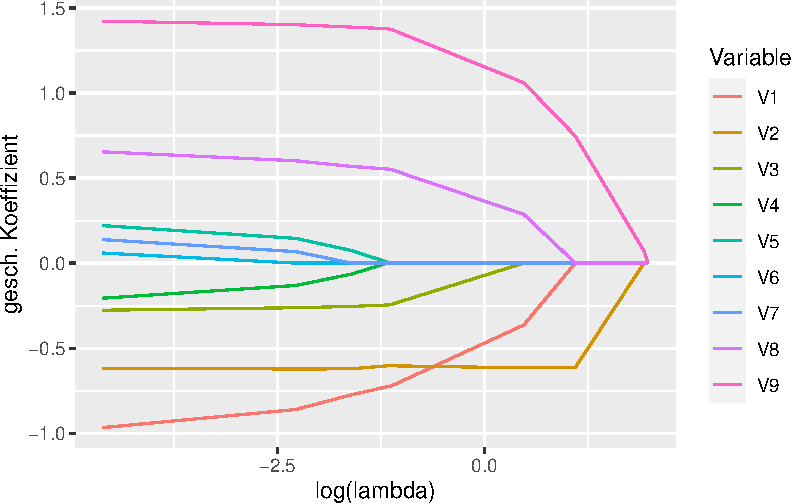
\includegraphics{RegReg_files/figure-pdf/fig-larssolpath-1.pdf}

}

\caption{\label{fig-larssolpath}LARS-Lösungspfad für Lasso-Schätzung}

\end{figure}%

Abbildung~\ref{fig-larssolpath} zeigt, dass die Shrinkage der
geschätzten Koeffizienten nach der Aktivierung rasch abnimmt und sich
für kleine Werte von \(\lambda\) der KQ-Lösung annähert. Wir sehen auch,
dass es einen Bereich von \(\lambda\)-Werten gibt, für die das wahre
Modell mit den Variablen \(X_1\), \(X_2\), \(X_8\) und \(X_9\)
selektiert werden kann. Je nach Ziel der Analyse kann es sinnvoll sein,
ein \(\lambda\) in diesem Intervall zu schätzen.

\subsection{\texorpdfstring{Wahl des Regularisierungsparameters
\(\lambda\) für den
Lasso-Schätzer}{Wahl des Regularisierungsparameters \textbackslash lambda für den Lasso-Schätzer}}\label{wahl-des-regularisierungsparameters-lambda-fuxfcr-den-lasso-schuxe4tzer}

Wie zuvor bei Ridge Regression muss in empirischen Anwendungen ein Wert
für den Tuning-Parameter \(\lambda\) gewählt werden. Hierbei besteht die
Herausforderung darin, einen geeigneten Wert zu finden, der zu
wünschenswerten Eigenschaften des resultierenden Modells führt. So ist
für gute Vorhersagen wichtig, dass das Modell nicht zu sehr an die Daten
angepasst ist (\emph{Overfitting}), um eine gute Generalisierung auf
neue Daten zu ermöglichen. Gleichzeitig muss das Modell flexibel genug
sein, um wesentliche Eigenschaften des datenerzeugenden Prozesses
hinreichend gut zu erfassen. In der Regel wird hierbei eine sparsame
Modellierung angestrebt, die nur eine Teilmenge der Prädiktoren nutzt.

In der Praxis werden verschiedene Verfahren verwendet, um den Wert für
den Tuning-Parameter \(\lambda\) zu bestimmen. Gängige Methoden sind
\emph{Cross Validation} (CV) und Informationskriterien. In Abhängigkeit
der Methode und der Daten ergeben sich ober- oder unterparameterisierte
Modelle. Aufgrund der Implementierung im R-Paket \texttt{lars}
betrachten wir CV.\footnote{Chetverikov, Liao, and Chernozhukov (2020)
  zeigen, dass CV zu konsistenter Modellselektion führen kann.} Wir
zeigen nachfolgend anhand der simulierten Daten aus dem letzten
Abschnitt, wie für die LARS-Schätzung ein optimales \(\lambda\) mit
leave-one-out CV (LOO-CV) bestimmt werden kann. Hierzu nutzen wir
\texttt{lars::cv.lars()} unter Verwendung derselben Argumente wie zuvor
im Aufruf von \texttt{lars()}.

\begin{Shaded}
\begin{Highlighting}[]
\CommentTok{\# LARS{-}Lösungen mit CV evaluieren}
\NormalTok{fit\_lars\_cv }\OtherTok{\textless{}{-}} \FunctionTok{cv.lars}\NormalTok{(}
  \AttributeTok{x =}\NormalTok{ X, }
  \AttributeTok{y =}\NormalTok{ Y, }
  \AttributeTok{intercept =}\NormalTok{ F,}
  \AttributeTok{normalize =}\NormalTok{ T,}
  \AttributeTok{type =} \StringTok{"lasso"}\NormalTok{, }
  \AttributeTok{plot.it =}\NormalTok{ F, }
  \AttributeTok{K =}\NormalTok{ N }\CommentTok{\# für LOO{-}CV}
\NormalTok{) }
\end{Highlighting}
\end{Shaded}

Das Objekt \texttt{fit\_lars\_cv} ist eine Liste mit den CV-Ergebnissen.
Wir können diese einfach mit \texttt{ggplot} visualisieren.
\texttt{index} ist hierbei das Verhältnis der \(\ell_1\)-Norm des
Lasso-Schätzers für einen spezifischen Wert von \(\lambda\) und der
\(\ell_1\)-Norm des KQ-Schätzers. Das optimale \(\lambda\) wird so
implizit geschätzt. \texttt{cv.error} ist der mit CV geschätzte MSE.

\begin{Shaded}
\begin{Highlighting}[]
\CommentTok{\# CV{-}MSE}
\NormalTok{fit\_lars\_cv }\SpecialCharTok{\%\textgreater{}\%} 
  \FunctionTok{as\_tibble}\NormalTok{() }\SpecialCharTok{\%\textgreater{}\%}

  \FunctionTok{ggplot}\NormalTok{(}
    \AttributeTok{mapping =} \FunctionTok{aes}\NormalTok{(}
      \AttributeTok{x =}\NormalTok{ index, }
      \AttributeTok{y =}\NormalTok{ cv.error}
\NormalTok{    )}
\NormalTok{  ) }\SpecialCharTok{+} 
  \FunctionTok{geom\_line}\NormalTok{() }\SpecialCharTok{+}
  \FunctionTok{xlab}\NormalTok{(}\StringTok{"|beta\_lambda| / |beta|"}\NormalTok{) }\SpecialCharTok{+}
  \FunctionTok{ylab}\NormalTok{(}\StringTok{"CV{-}MSE"}\NormalTok{)}
\end{Highlighting}
\end{Shaded}

\begin{figure}[t]

\centering{

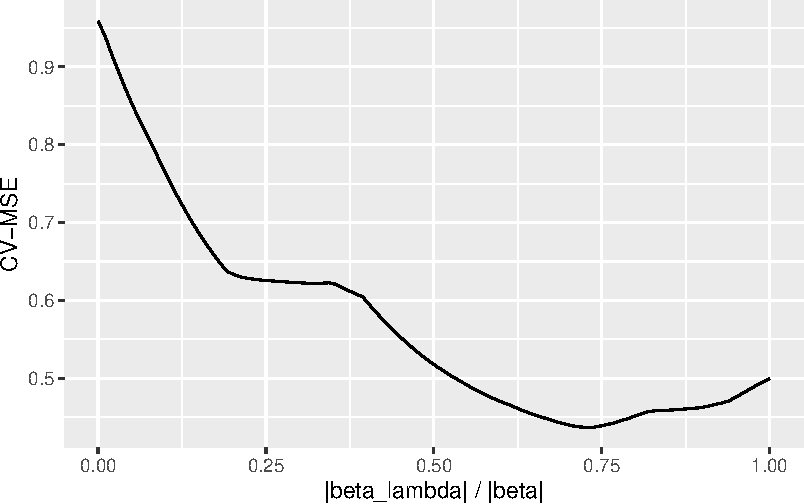
\includegraphics{RegReg_files/figure-pdf/fig-larscv-1.pdf}

}

\caption{\label{fig-larscv}CV-MSE und relative Position von \(\lambda\)
auf dem Lassopfad}

\end{figure}%

In der Grafik erkennen wir ein Minimum des CV-MSEs bei etwa 0.73.

\begin{Shaded}
\begin{Highlighting}[]
\CommentTok{\# CV{-}MSE{-}minimierendes Lambda bestimmen}
\NormalTok{ID }\OtherTok{\textless{}{-}} \FunctionTok{which.min}\NormalTok{(fit\_lars\_cv}\SpecialCharTok{$}\NormalTok{cv.error) }\CommentTok{\# Index}

\NormalTok{(}
\NormalTok{  fraction\_opt }\OtherTok{\textless{}{-}}\NormalTok{ fit\_lars\_cv}\SpecialCharTok{$}\NormalTok{index[ID]}
\NormalTok{)}
\end{Highlighting}
\end{Shaded}

\begin{verbatim}
[1] 0.7272727
\end{verbatim}

Die geschätzten Koeffizienten für die optimale Regularisierung können
mit \texttt{coef()} ausgelesen werden.

\begin{Shaded}
\begin{Highlighting}[]
\CommentTok{\# LARS{-}Lasso{-}Fit für optimales lambda bestimmen}
\FunctionTok{coef}\NormalTok{(}
  \AttributeTok{object =}\NormalTok{ fit\_lars, }
  \AttributeTok{s =}\NormalTok{ fraction\_opt, }
  \AttributeTok{mode =} \StringTok{"fraction"}
\NormalTok{)}
\end{Highlighting}
\end{Shaded}

\begin{verbatim}
[1] -0.6513191 -0.6060906 -0.1946089  0.0000000  0.0000000  0.0000000  0.0000000
[8]  0.4977908  1.3122407
\end{verbatim}

Das Ergebnis veranschaulicht die Selektionseigenschaft von Lasso: Gemäß
DGP \eqref{eq:larsdgp} sind die Variablen \(X_3\) bis \(X_7\)
\emph{irrelevante} Prädiktoren für \(Y\); ihre wahren Koeffizienten sind
\(0\). In der kreuzvalidierten Lasso-Schätzung erreicht die
Regularisierung, dass die Koeffizienten der Variablen \(X_4\) bis
\(X_7\) tatsächlich mit 0 geschätzt werden. Wir schätzen für das mit CV
bestimmte \(\lambda\) also ein leicht überspezifiziertes Modell mit den
Regressoren \(X_1\), \(X_2\), \(X_3\), \(X_8\) und \(X_9\). Beachte,
dass die Lasso-Schätzung einen Kompromiss impliziert: Die Varianz der
Schätzung ist geringer als die des KQ-Schätzers im Modell mit allen
Variablen.\footnote{Wegen \(N=25\) verbleiben bei der KQ-Schätzung mit 9
  Regressoren nur 16 Freiheitsgrade.} Aufgrund der Regularisierung sind
die mit Lasso geschätzten Koeffizienten der relevanten Variablen jedoch
in Richtung \(0\) verzerrt.

Einen positiven Effekt dieses Kompromisses beobachten wir anhand des
mittleren Vorhersagefehlers für Daten, die \emph{nicht} zur Berechnung
des Schätzers verwendet wurden. Wir vergleichen den Vorhersagefehler
nachfolgend anhand eines solchen simulierten Test-Datensatzes mit 25
neuen Beobachtungen. Den Vorhersagefehler bestimmen wir als MSE zwischen
den vorhergesagten und den tatsächlichen Ausprägungen für \(Y\).

\begin{Shaded}
\begin{Highlighting}[]
\CommentTok{\# Test{-}Datensatz erstellen}
\FunctionTok{set.seed}\NormalTok{(}\DecValTok{4321}\NormalTok{)}
\NormalTok{new\_X }\OtherTok{\textless{}{-}} \FunctionTok{matrix}\NormalTok{(}\FunctionTok{rnorm}\NormalTok{(N }\SpecialCharTok{*} \DecValTok{9}\NormalTok{), }\AttributeTok{ncol =} \DecValTok{9}\NormalTok{)}
\NormalTok{new\_Y }\OtherTok{\textless{}{-}}\NormalTok{ new\_X }\SpecialCharTok{\%*\%}\NormalTok{ beta\_v }\SpecialCharTok{+} \FunctionTok{rnorm}\NormalTok{(N)}

\CommentTok{\# Lasso: Vorhersage von new\_Y für Test{-}Datensatz}
\NormalTok{Y\_predict\_lars }\OtherTok{\textless{}{-}} \FunctionTok{predict}\NormalTok{(}
  \AttributeTok{object =}\NormalTok{ fit\_lars, }
  \AttributeTok{s =}\NormalTok{ fraction\_opt, }
  \AttributeTok{type =} \StringTok{"fit"}\NormalTok{, }
  \AttributeTok{mode =} \StringTok{"fraction"}\NormalTok{, }
  \AttributeTok{newx =}\NormalTok{ new\_X}
\NormalTok{)}\SpecialCharTok{$}\NormalTok{fit}

\CommentTok{\# Lasso: MSE für Test{-}Datensatz berechnen}
\FunctionTok{mean}\NormalTok{((Y\_predict\_lars }\SpecialCharTok{{-}}\NormalTok{ new\_Y)}\SpecialCharTok{\^{}}\DecValTok{2}\NormalTok{)}
\end{Highlighting}
\end{Shaded}

\begin{verbatim}
[1] 1.419817
\end{verbatim}

Wir schätzen nun das große Modell mit allen 9 Variablen mit KQ und
berechnen ebenfalls den MSE der Prognosen für den Test-Datensatz.

\begin{Shaded}
\begin{Highlighting}[]
\CommentTok{\# KQ{-}Schätzung des großen Modells durchführen}
\NormalTok{KQ\_fit }\OtherTok{\textless{}{-}} \FunctionTok{lm}\NormalTok{(Y }\SpecialCharTok{\textasciitilde{}}\NormalTok{ X }\SpecialCharTok{{-}} \DecValTok{1}\NormalTok{)}

\CommentTok{\# Test{-}Datensatz für predict.lm() formatieren}
\NormalTok{new\_X }\OtherTok{\textless{}{-}} \FunctionTok{as.data.frame}\NormalTok{(new\_X)}
\FunctionTok{colnames}\NormalTok{(new\_X) }\OtherTok{\textless{}{-}} \FunctionTok{paste0}\NormalTok{(}\StringTok{"X"}\NormalTok{, }\DecValTok{1}\SpecialCharTok{:}\DecValTok{9}\NormalTok{)}

\CommentTok{\# KQ: Vorhersage von new\_Y für Test{-}Datensatz}
\NormalTok{Y\_predict\_KQ }\OtherTok{\textless{}{-}} \FunctionTok{predict}\NormalTok{(}
  \AttributeTok{object =}\NormalTok{ KQ\_fit, }
  \AttributeTok{newdata =}\NormalTok{ new\_X}
\NormalTok{)}

\CommentTok{\# KQ: MSE für Test{-}Datensatz berechnen}
\FunctionTok{mean}\NormalTok{((Y\_predict\_KQ }\SpecialCharTok{{-}}\NormalTok{ new\_Y)}\SpecialCharTok{\^{}}\DecValTok{2}\NormalTok{)}
\end{Highlighting}
\end{Shaded}

\begin{verbatim}
[1] 9.851932
\end{verbatim}

Offenbar führt die Lasso-Schätzung zu einem deutlich geringeren MSE der
Vorhersage von \texttt{Y} für den Test-Datensatz als die KQ-Schätzung
und damit zu einer höheren Vorhersagegüte. Das ``sparsame'' mit
Lasso-Regression geschätzte Modell ist dem ``großen'' mit KQ geschätztem
Modell in dieser Hinsicht also überlegen.

\begin{tcolorbox}[enhanced jigsaw, bottomtitle=1mm, colbacktitle=quarto-callout-note-color!10!white, coltitle=black, arc=.35mm, title=\textcolor{quarto-callout-note-color}{\faInfo}\hspace{0.5em}{Key Facts zu Lasso-Regression}, titlerule=0mm, opacityback=0, breakable, bottomrule=.15mm, toprule=.15mm, opacitybacktitle=0.6, colframe=quarto-callout-note-color-frame, toptitle=1mm, rightrule=.15mm, leftrule=.75mm, left=2mm, colback=white]

\begin{itemize}
\item
  Lasso-Regression bestraft die Verlustfunktion des KQ-Schätzers mit der
  \(\ell_1\)-Norm der Koeffizienten.
\item
  Neben Koeffizientenschätzung mit Shrinkage in Richtung \(0\) kann der
  Lasso-Schätzer Variablenselektion durchführen:
  Regressionskoeffizienten können exakt mit \(0\) geschätzt und so ein
  ``sparsames'', leichter zu interpretierendes Modell gewählt werden.
\item
  Wie bei Ridge Regression impliziert die Wahl von \(\lambda\) einen
  Bias-Variance-Tradeoff, der für Vorhersagen nützlich ist: Für größere
  \(\lambda\) wird mehr Verzerrung induziert und möglicherweise
  relevante Variablen mit kleinen Koeffizienten aus dem Modell entfernt.
  Ein solches sparsames Modell kann eine höhere Prognosegüte haben als
  ein komplexes, unregularisiertes Modell.
\item
  Der Lasso-Schätzer \(\widehat{\boldsymbol{\beta}}_\lambda^L\) ist
  \emph{nicht} erwartungstreu.
\item
  Lasso Regression kann bspw. mit dem LARS-Algorithmus (Paket
  \texttt{lars}) oder mit \texttt{glmnet} berechnet werden.
\end{itemize}

\end{tcolorbox}

\section{Vergleich von Lasso- und Ridge-Regression mit
Simulation}\label{vergleich-von-lasso--und-ridge-regression-mit-simulation}

In diesem Kapitel illustrieren wir Vor- und Nachteile von Lasso- und
Ridge-Regression in Prognose-Anwendungen anhand von
Monte-Carlo-Simulationen. Wir betrachten hierbei datenerzeugende
Prozesse, die sich hinsichtlich der Anzahl relevanter Variablen sowie
der Korrelation dieser Variablen unterscheiden.

Die grundlegende Vorschrift für die Simulationen ist \begin{align*}
  Y_i = \sum_{j=1}^{k=40} \beta_j X_{i,j} + u_i, \quad u_i \overset{u.i.v.}{\sim} N(0,1), \quad i=1,\dots,100,
\end{align*} wobei die Regressoren \(X_j\) eine Varianz von \(1\) haben
und aus einer multivariaten Normalverteilung mit Korrelation
\[\rho\in(0,0.5,0.8)\] gezogen werden.

Für die Koeffizienten \(\boldsymbol{\beta}\) unterscheiden wir zwei
Szenarien. In Szenario A ist \[\boldsymbol{\beta} = (1,\dots,1)',\] d.h.
alle Variablen sind relevant und haben denselben Einfluss auf \(Y\). In
Szenario B erzeugen wir \(\boldsymbol{\beta}\) einmalig vorab so, dass
\[\beta_j = \begin{cases}1,\quad \text{mit Wsk.  }p\\ 0,\quad \text{mit Wsk.  }1-p, \end{cases}\]
d.h. nur eine Teilmenge der Variablen beeinflusst \(Y\) jeweils mit
demselben Effekt \(\beta_j = 1\). Die übrigen Variablen sind irrelevant.

Wir schätzen und validieren die Modelle mit \texttt{glmnet()}.

\subsection{Prognosegüte in diversen Szenarien}\label{sec-pdz}

\begin{Shaded}
\begin{Highlighting}[]
\CommentTok{\# Simulationsparameter definieren}
\NormalTok{rho }\OtherTok{\textless{}{-}} \FunctionTok{c}\NormalTok{(}\DecValTok{0}\NormalTok{, }\FloatTok{0.5}\NormalTok{, }\FloatTok{0.8}\NormalTok{)   }\CommentTok{\# Korrelation}
\NormalTok{k }\OtherTok{\textless{}{-}} \DecValTok{40}                 \CommentTok{\# Anz. Regressoren}
\NormalTok{N }\OtherTok{\textless{}{-}} \DecValTok{100}                \CommentTok{\# Anz. Beobachtungen}
\NormalTok{n\_sim }\OtherTok{\textless{}{-}} \DecValTok{100}            \CommentTok{\# Anz. Simulationen}
\end{Highlighting}
\end{Shaded}

Damit der Code für die Simulation möglichst wenig repetitiv ist,
definieren wir eine Funktion \texttt{cv.glmnet\_MSE()}, die unter Angabe
der Daten \texttt{X} und \texttt{Y}, des Trainingssets \texttt{train}
sowie des Parameters \texttt{alpha} den gewünschten regularisierten
Schätzer under Verwendung von Cross Validation anpasst und den
Testset-MSE zurückgibt.

\begin{Shaded}
\begin{Highlighting}[]
\CommentTok{\# allg. Funktion für Testset{-}MSE nach CV}
\NormalTok{cv.glmnet\_MSE }\OtherTok{\textless{}{-}} \ControlFlowTok{function}\NormalTok{(X, Y, train, alpha) \{}
  
  \CommentTok{\# Modell mit glmnet schätzen; lambda per CV bestimmen}
\NormalTok{  fit\_cv }\OtherTok{\textless{}{-}} \FunctionTok{cv.glmnet}\NormalTok{(}
    \AttributeTok{x =}\NormalTok{ X[train,],}
    \AttributeTok{y =}\NormalTok{Y[train],}
    \AttributeTok{alpha =}\NormalTok{ alpha}
\NormalTok{  )}
  
  \CommentTok{\# Vorhersagen treffen}
\NormalTok{  Y\_pred }\OtherTok{\textless{}{-}} \FunctionTok{predict}\NormalTok{(}
    \AttributeTok{object =}\NormalTok{ fit\_cv, }
    \AttributeTok{s =}\NormalTok{ fit\_cv}\SpecialCharTok{$}\NormalTok{lambda.min, }
    \AttributeTok{newx =}\NormalTok{ X[}\SpecialCharTok{{-}}\NormalTok{train,])}
  
  \FunctionTok{return}\NormalTok{(}
    \CommentTok{\# Testset{-}MSE berechnen}
    \FunctionTok{mean}\NormalTok{(}
\NormalTok{      (Y[}\SpecialCharTok{{-}}\NormalTok{train] }\SpecialCharTok{{-}}\NormalTok{ Y\_pred)}\SpecialCharTok{\^{}}\DecValTok{2}
\NormalTok{      )}
\NormalTok{  )}
\NormalTok{\}}
\end{Highlighting}
\end{Shaded}

Wir initialisieren zunächst Matrizen, in welche die MSEs aus den 100
Simulationsdurchläufen reihenweise geschrieben werden.
\texttt{lasso\_mse} und \texttt{ridge\_mse} haben je eine Spalte für
jede Korrelation in \texttt{rho}

\begin{Shaded}
\begin{Highlighting}[]
\CommentTok{\# Matrizen für simulierte MSEs initialisieren...}
\NormalTok{lasso\_mse }\OtherTok{\textless{}{-}} \FunctionTok{matrix}\NormalTok{(}
  \AttributeTok{data =} \ConstantTok{NA}\NormalTok{, }
  \AttributeTok{nrow =}\NormalTok{ n\_sim, }
  \AttributeTok{ncol =} \FunctionTok{length}\NormalTok{(rho)}
\NormalTok{) }
\NormalTok{ridge\_mse }\OtherTok{\textless{}{-}}\NormalTok{ lasso\_mse}

\CommentTok{\# ... und benennen}
\FunctionTok{colnames}\NormalTok{(lasso\_mse) }\OtherTok{\textless{}{-}} \FunctionTok{paste0}\NormalTok{(}\StringTok{"Kor="}\NormalTok{, rho)}
\FunctionTok{colnames}\NormalTok{(ridge\_mse) }\OtherTok{\textless{}{-}} \FunctionTok{colnames}\NormalTok{(lasso\_mse)}
\end{Highlighting}
\end{Shaded}

Für die Simulation iterieren wir mit \texttt{purrr::walk} über den
Vektor \texttt{rho} sowie über die Laufvariable \texttt{1:n\_sim}. Beide
Schleifen nutzen den Syntax für anonyme Funktionen:

\begin{Shaded}
\begin{Highlighting}[]
\CommentTok{\# Die anonyme Funktion}
\ControlFlowTok{function}\NormalTok{(x) }\FunctionTok{return}\NormalTok{(x)}
\CommentTok{\# ist äquivalent definiert als}
\NormalTok{\textbackslash{}(x) }\FunctionTok{return}\NormalTok{(x)}
\end{Highlighting}
\end{Shaded}

In jeden Simulationsdurchlauf erzeugen wir den Datensatz entsprechend
der obigen Vorschrift, teilen die Daten auf und berechnen MSEs für
Lasso- und Ridge-Regression mit \texttt{cv.glmnet\_MSE()}.

\textbf{Szenario A}

\begin{Shaded}
\begin{Highlighting}[]
\CommentTok{\# Koeffizienten{-}Vektor definieren}
\NormalTok{beta }\OtherTok{\textless{}{-}} \FunctionTok{rep}\NormalTok{(}\DecValTok{1}\NormalTok{, k) }
\end{Highlighting}
\end{Shaded}

\begin{Shaded}
\begin{Highlighting}[]
\FunctionTok{library}\NormalTok{(mvtnorm)}
\FunctionTok{library}\NormalTok{(tidyverse)}

\FunctionTok{set.seed}\NormalTok{(}\DecValTok{1234}\NormalTok{)}

\CommentTok{\# Simulation durchführen}
\FunctionTok{walk}\NormalTok{(}\DecValTok{1}\SpecialCharTok{:}\FunctionTok{length}\NormalTok{(rho), \textbackslash{}(j) \{}
  
  \CommentTok{\# Korrelationsmatrix definieren}
\NormalTok{  Sigma }\OtherTok{\textless{}{-}} \FunctionTok{matrix}\NormalTok{(}
    \AttributeTok{data =}\NormalTok{ rho[j], }
    \AttributeTok{nrow =}\NormalTok{ k, }
    \AttributeTok{ncol =}\NormalTok{ k}
\NormalTok{  )}
  \FunctionTok{diag}\NormalTok{(Sigma) }\OtherTok{\textless{}{-}} \DecValTok{1}
  
  \FunctionTok{walk}\NormalTok{(}\DecValTok{1}\SpecialCharTok{:}\NormalTok{n\_sim, \textbackslash{}(i) \{}
    
  \CommentTok{\# Daten simulieren}
\NormalTok{  X }\OtherTok{\textless{}{-}} \FunctionTok{rmvnorm}\NormalTok{(}
    \AttributeTok{n =}\NormalTok{ N, }
    \AttributeTok{mean =} \FunctionTok{rep}\NormalTok{(}\DecValTok{0}\NormalTok{, k), }
    \AttributeTok{sigma =}\NormalTok{ Sigma}
\NormalTok{  )}
\NormalTok{  Y }\OtherTok{\textless{}{-}}\NormalTok{ X }\SpecialCharTok{\%*\%}\NormalTok{ beta }\SpecialCharTok{+} \FunctionTok{rnorm}\NormalTok{(N)}
    
  \CommentTok{\# Trainingsdaten definieren}
\NormalTok{  ID\_train }\OtherTok{\textless{}{-}} \FunctionTok{sample}\NormalTok{(}
    \AttributeTok{x =} \FunctionTok{c}\NormalTok{(}\DecValTok{1}\SpecialCharTok{:}\NormalTok{N), }
    \AttributeTok{size =}\NormalTok{ N}\SpecialCharTok{/}\DecValTok{2}
\NormalTok{  )}
    
  \CommentTok{\# Modelle mit CV schätzen und MSEs berechnen}
  \CommentTok{\# Ridge{-}Regression}
\NormalTok{  ridge\_mse[i, j] }\OtherTok{\textless{}\textless{}{-}} \FunctionTok{cv.glmnet\_MSE}\NormalTok{(}
    \AttributeTok{X =}\NormalTok{ X, }
    \AttributeTok{Y =}\NormalTok{ Y, }
    \AttributeTok{train =}\NormalTok{ ID\_train, }
    \AttributeTok{alpha =} \DecValTok{0}
\NormalTok{  )}
  
  \CommentTok{\# Lasso{-}Regression}
\NormalTok{  lasso\_mse[i, j] }\OtherTok{\textless{}\textless{}{-}} \FunctionTok{cv.glmnet\_MSE}\NormalTok{(}
    \AttributeTok{X =}\NormalTok{ X, }
    \AttributeTok{Y =}\NormalTok{ Y, }
    \AttributeTok{train =}\NormalTok{ ID\_train, }
    \AttributeTok{alpha =} \DecValTok{1}
\NormalTok{  )}
  
\NormalTok{  \})}
  
\NormalTok{\})}
\end{Highlighting}
\end{Shaded}

Beachte, dass hier der Super-Assignment-Operator
\texttt{\textless{}\textless{}-} genutzt wird, damit \texttt{walk} die
Matrizen \texttt{ridge\_mse} und \texttt{lasso\_mse} in der globalen
Umgebung überschreibt.\footnote{Dies folgt aus der Definition von
  \texttt{walk}. \texttt{\textless{}-} bewirkt hier lediglich Assignment
  in der Funktionsumgebung.}

Wir berechnen jeweils den mittleren MSEs, sammeln die Ergebnisse in
einer \texttt{tibble()} und nutzen \texttt{gt()} für die tabellarische
Darstellung.

\begin{Shaded}
\begin{Highlighting}[]
\FunctionTok{library}\NormalTok{(gt)}

\CommentTok{\# Ergebnisse tabellarisch darstellen}
\FunctionTok{tibble}\NormalTok{(}
  \AttributeTok{Methode =} \FunctionTok{c}\NormalTok{(}
    \StringTok{"Lasso{-}Regression"}\NormalTok{, }
    \StringTok{"Ridge{-}Regression"}
\NormalTok{  ),}
\NormalTok{) }\SpecialCharTok{\%\textgreater{}\%}
  \FunctionTok{bind\_cols}\NormalTok{(}
    \FunctionTok{bind\_rows}\NormalTok{(}
      \FunctionTok{colMeans}\NormalTok{(lasso\_mse),}
      \FunctionTok{colMeans}\NormalTok{(ridge\_mse)  }
\NormalTok{    )    }
\NormalTok{  ) }\SpecialCharTok{\%\textgreater{}\%}
  \FunctionTok{gt}\NormalTok{() }\SpecialCharTok{\%\textgreater{}\%}
\NormalTok{  tabopts}
\end{Highlighting}
\end{Shaded}

\begin{longtable}{lrrr}

\caption{\label{tbl-lrsimA}Durchschnittliche Testset-MSEs für Setting A}

\tabularnewline

\toprule
Methode & Kor=0 & Kor=0.5 & Kor=0.8 \\ 
\midrule\addlinespace[2.5pt]
Lasso-Regression & $7.17$ & $10.398$ & $7.581$ \\ 
Ridge-Regression & $4.841$ & $1.615$ & $1.517$ \\ 
\bottomrule

\end{longtable}

Tabelle~\ref{tbl-lrsimA} zeigt, dass Ridge-Regression gegenüber
Lasso-Regression für jede der drei betrachteten Korrelationen überlegen
ist. Insbesondere bei stärker korrelierten Regressoren ist Ridge
vorteilhaft.

Für Szenario B überschreiben wir \texttt{beta} nach Multiplikation mit
einem zufälligen binären Vektor, sodass einige der Koeffizienten \(0\)
und die zugehörigen Variablen irrelevant für \(Y\) sind.

\textbf{Szenario B}

\begin{Shaded}
\begin{Highlighting}[]
\CommentTok{\# Wsk. für Relevanz einer Variable}
\NormalTok{p }\OtherTok{\textless{}{-}}\NormalTok{ .}\DecValTok{3}

\CommentTok{\# Koeffizienten{-}Vektor definieren}
\FunctionTok{set.seed}\NormalTok{(}\DecValTok{123}\NormalTok{)}
\NormalTok{beta }\OtherTok{\textless{}{-}}\NormalTok{ beta }\SpecialCharTok{*} \FunctionTok{sample}\NormalTok{(}
  \AttributeTok{x =} \DecValTok{0}\SpecialCharTok{:}\DecValTok{1}\NormalTok{, }
  \AttributeTok{size =}\NormalTok{ k, }
  \AttributeTok{replace =}\NormalTok{ T, }
  \AttributeTok{prob =} \FunctionTok{c}\NormalTok{(}\DecValTok{1}\SpecialCharTok{{-}}\NormalTok{p, p)}
\NormalTok{)}

\CommentTok{\# Koeffizienten prüfen}
\FunctionTok{head}\NormalTok{(beta, }\AttributeTok{n =} \DecValTok{10}\NormalTok{)}
\end{Highlighting}
\end{Shaded}

\begin{verbatim}
 [1] 0 1 0 1 1 0 0 1 0 0
\end{verbatim}

Eine wiederholung der Simulation für die modifizierten Koeffizienten
\texttt{beta} und liefert folgende tabellarische Auswertung.

\begin{longtable}{lrrr}

\caption{\label{tbl-lrsimB}Durchschnittliche Testset-MSEs für Szenario
B}

\tabularnewline

\toprule
Methode & Kor=0 & Kor=0.5 & Kor=0.8 \\ 
\midrule\addlinespace[2.5pt]
Lasso & $2.51$ & $2.143$ & $1.923$ \\ 
Ridge & $3.331$ & $2.562$ & $2.014$ \\ 
\bottomrule

\end{longtable}

Die Ergebnisse in Tabelle~\ref{tbl-lrsimB} zeigen, dass Ridge-Regression
in Szenario B bis auf den Fall unkorrelierter Regressoren etwas
schlechter abschneidet als in Szenario A. Die hohe Anzahl irrelevanter
Variablen verbessert die Leistung von Lasso deutlich: Hier ist es
plausibel, dass Lasso aufgrund der Thresholding-Eigenschaft die
Koeffizienten einiger irrelevanten Variablen häufig exakt \(0\) setzt
und damit ein sparsameres Modell schätzt als Ridge. Entsprechend erzielt
Lasso in diesem Szenario insbesondere für \(\rho = 0\) genauere
Vorhersagen als Ridge Regression.

\subsection{Visualisierung des Bias-Variance-Tradeoffs bei
Prognosen}\label{visualisierung-des-bias-variance-tradeoffs-bei-prognosen}

Für ein besseres Verständnis, wie sich der Regularisierungsparameter
\(\lambda\) auf den Bias-Variance-Tradeoff bei Prognosen mit Ridge- und
Lasso-Regression auswirkt, vergleichen wir für beide Methoden
nachfolgend die Abhängigkeit des MSEs der Prognose \(\widehat{Y}_0\) für
den Wert \(Y_0\) der abhängigen Variable eines Datenpunkts anhand seiner
Regressoren \(\boldsymbol{X}_0'\), wobei \begin{align}
  \text{MSE}(\widehat{Y}_0) = \text{Bias}(\widehat{Y}_0)^2 + \text{Var}(\widehat{Y}_0) + \text{Var}(Y_0) \label{eq:pbvdecomp}
\end{align} Beachte, dass \(\text{Var}(Y_0)\) die durch den
datenerzeugenden Prozess (und damit unvermeidbare) Varianz von \(Y_0\)
ist, wohingegen \(\text{Bias}(\widehat{Y}_0)^2\) und
\(\text{Var}(\widehat{Y}_0)\) von dem verwendeten Schätzer für
\(\widehat{Y}_0\) abhängt.

Für die Simulation betrachten wir erneut Szenario A aus
Kapitel~\ref{sec-pdz} mit \(50\) Beobachtungen für ein Modell mit \(40\)
unkorrelierten Regressoren. Wir legen zunächst die Simulationsparameter
fest und erzeugen den vorherzusagenden Datenpunkt (\texttt{X\_0},
\texttt{Y\_0}).

\begin{Shaded}
\begin{Highlighting}[]
\CommentTok{\# Parameter festlegen}
\FunctionTok{set.seed}\NormalTok{(}\DecValTok{1234}\NormalTok{)}
\NormalTok{n }\OtherTok{\textless{}{-}} \DecValTok{200} \CommentTok{\# Anz. Iterationen}
\NormalTok{N }\OtherTok{\textless{}{-}} \DecValTok{50}  \CommentTok{\# Anz. Beobachtungen}
\NormalTok{k }\OtherTok{\textless{}{-}} \DecValTok{40}  \CommentTok{\# Anz. Variablen}

\CommentTok{\# Korrelationsmatrix definieren}
\NormalTok{Sigma }\OtherTok{\textless{}{-}} \FunctionTok{diag}\NormalTok{(k) }\CommentTok{\# Diagonalmatrix}
\NormalTok{beta }\OtherTok{\textless{}{-}} \FunctionTok{rep}\NormalTok{(}\AttributeTok{x =} \DecValTok{1}\NormalTok{, k)}

\CommentTok{\# Prognose{-}Ziel vorab zufällig generieren:}

\CommentTok{\# Regressoren}
\NormalTok{X\_0 }\OtherTok{\textless{}{-}} \FunctionTok{rmvnorm}\NormalTok{(}
  \AttributeTok{n =} \DecValTok{1}\NormalTok{, }
  \AttributeTok{mean =} \FunctionTok{rep}\NormalTok{(}\AttributeTok{x =} \DecValTok{0}\NormalTok{, k)}
\NormalTok{)}

\CommentTok{\# Abh. Variable}
\NormalTok{Y\_0 }\OtherTok{\textless{}{-}}\NormalTok{ X\_0 }\SpecialCharTok{\%*\%}\NormalTok{ beta }\SpecialCharTok{+} \FunctionTok{rnorm}\NormalTok{(}\AttributeTok{n =} \DecValTok{1}\NormalTok{) }\SpecialCharTok{\%\textgreater{}\%} 
  \FunctionTok{as.vector}\NormalTok{()}
\end{Highlighting}
\end{Shaded}

Anhand der Simulationsergebnisse wollen wir die von der verwendeten
Schätzfunktion abhängigen Komponenten von \eqref{eq:pbvdecomp}
untersuchen. Wir initialisieren hierzu die Listen \texttt{ridge\_fits}
und \texttt{lasso\_fits}, in die unsere Simulationsergebnisse
geschrieben werden.

\begin{Shaded}
\begin{Highlighting}[]
\CommentTok{\# Listen für Simulationsergebnisse initialisieren}
\NormalTok{ridge\_fits }\OtherTok{\textless{}{-}} \FunctionTok{list}\NormalTok{()}
\NormalTok{lasso\_fits }\OtherTok{\textless{}{-}} \FunctionTok{list}\NormalTok{()}
\end{Highlighting}
\end{Shaded}

Weiterhin definieren wir separate \(\lambda\)-Sequenzen für Lasso- und
Ridge-Schätzer.\footnote{Die Sequenzen haben wir in Abhängigkeit des DGP
  so gewählt, dass die Abhängigkeit der Prognosegüte von \(\lambda\) gut
  visualisiert werden kann.}

\begin{Shaded}
\begin{Highlighting}[]
\CommentTok{\# Lambda{-}Sequenzen festlegen}
\NormalTok{lambdas\_r }\OtherTok{\textless{}{-}} \FunctionTok{seq}\NormalTok{(.}\DecValTok{25}\NormalTok{, }\FloatTok{2.5}\NormalTok{, }\AttributeTok{length.out =} \DecValTok{100}\NormalTok{)}
\NormalTok{lambdas\_l }\OtherTok{\textless{}{-}} \FunctionTok{seq}\NormalTok{(.}\DecValTok{05}\NormalTok{, }\FloatTok{0.5}\NormalTok{, }\AttributeTok{length.out =} \DecValTok{100}\NormalTok{)}
\end{Highlighting}
\end{Shaded}

Für die Simulation iterieren wir mit \texttt{walk()} über simulierte
Datensätze und schreiben jeweils den vollständigen Output von
\texttt{glmnet()} in die zuvor definierten Listen \texttt{ridge\_fits}
und \texttt{lasso\_fits}.

\begin{Shaded}
\begin{Highlighting}[]
\CommentTok{\# Simulation}
\FunctionTok{walk}\NormalTok{(}\DecValTok{1}\SpecialCharTok{:}\NormalTok{n, \textbackslash{}(i) \{}
  
  \CommentTok{\# Daten simulieren}
\NormalTok{  X }\OtherTok{\textless{}{-}} \FunctionTok{rmvnorm}\NormalTok{(}
    \AttributeTok{n =}\NormalTok{ N, }
    \AttributeTok{mean =} \FunctionTok{rep}\NormalTok{(}\DecValTok{0}\NormalTok{, k), }
    \AttributeTok{sigma =}\NormalTok{ Sigma}
\NormalTok{  )}
\NormalTok{  Y }\OtherTok{\textless{}{-}}\NormalTok{ X }\SpecialCharTok{\%*\%}\NormalTok{ beta }\SpecialCharTok{+} \FunctionTok{rnorm}\NormalTok{(}\AttributeTok{n =}\NormalTok{ N, }\AttributeTok{sd =} \DecValTok{5}\NormalTok{)}
  
  \CommentTok{\# Modelle mit glmnet schätzen}
  \CommentTok{\# Ridge{-}Regression}
\NormalTok{  ridge\_fits[[i]] }\OtherTok{\textless{}\textless{}{-}} \FunctionTok{glmnet}\NormalTok{(}
    \AttributeTok{x =}\NormalTok{ X, }
    \AttributeTok{y =}\NormalTok{ Y, }
    \AttributeTok{alpha =} \DecValTok{0}\NormalTok{, }
    \AttributeTok{intercept =}\NormalTok{ F}
\NormalTok{  )}
  \CommentTok{\# Lasso{-}Regression}
\NormalTok{  lasso\_fits[[i]] }\OtherTok{\textless{}\textless{}{-}} \FunctionTok{glmnet}\NormalTok{(}
    \AttributeTok{x =}\NormalTok{ X, }
    \AttributeTok{y =}\NormalTok{ Y, }
    \AttributeTok{alpha =} \DecValTok{1}\NormalTok{, }
    \AttributeTok{intercept =}\NormalTok{ F}
\NormalTok{  )}
  
\NormalTok{\})}
\end{Highlighting}
\end{Shaded}

Wir nutzen Funktionen aus \texttt{purrr} und \texttt{dplyr}, um über die
in den Simulationsdurchläufen angepassten Modelle zu iterieren. Mit
\texttt{predict()} erhalten wir Punktvorhersagen für \texttt{Y\_0} für
jedes \(\lambda\) der zuvor definierten \(\lambda\)-Sequenzen. Beachte,
dass \texttt{map()} jeweils eine Liste mit 200 Punktvorhersagen für
jedes der 100 zurückgibt. Mit \texttt{list\_rbind()} können wir die
Ergebnisse komfortabel jeweils in einer \texttt{tibble} sammeln.

\begin{Shaded}
\begin{Highlighting}[]
\CommentTok{\# Prognosen für Ridge{-}Regression}
\NormalTok{pred\_r }\OtherTok{\textless{}{-}} \FunctionTok{map}\NormalTok{(}
  \AttributeTok{.x =}\NormalTok{ ridge\_fits, }
  \AttributeTok{.f =} \SpecialCharTok{\textasciitilde{}} \FunctionTok{as\_tibble}\NormalTok{(}
    \FunctionTok{predict}\NormalTok{(}
      \AttributeTok{object =}\NormalTok{ ., }
      \AttributeTok{s =}\NormalTok{ lambdas\_r, }
      \AttributeTok{newx =}\NormalTok{ X\_0}
\NormalTok{    )}
\NormalTok{  ) }
\NormalTok{) }\SpecialCharTok{\%\textgreater{}\%}
  \FunctionTok{list\_rbind}\NormalTok{() }

\CommentTok{\# Prognosen für Lasso{-}Regression}
\NormalTok{pred\_l }\OtherTok{\textless{}{-}} \FunctionTok{map}\NormalTok{(}
  \AttributeTok{.x =}\NormalTok{ lasso\_fits, }
  \AttributeTok{.f =} \SpecialCharTok{\textasciitilde{}} \FunctionTok{as\_tibble}\NormalTok{(}
    \FunctionTok{predict}\NormalTok{(}
      \AttributeTok{object =}\NormalTok{ ., }
      \AttributeTok{s =}\NormalTok{ lambdas\_l, }
      \AttributeTok{newx =}\NormalTok{ X\_0)}
\NormalTok{    ) }
\NormalTok{) }\SpecialCharTok{\%\textgreater{}\%}
  \FunctionTok{list\_rbind}\NormalTok{() }
\end{Highlighting}
\end{Shaded}

Für die statistische Auswertung berechnen wir jeweils
\(\text{MSE}(\widehat{Y}_0)\), \(\text{Bias}(\widehat{Y}_0)^2\) und
\(\text{Var}(\widehat{Y}_0)\) und führen die Ergebnisse mit
\texttt{pivot\_longer()} in ein langes Format \texttt{sim\_data\_r}
über. Wir berechnen weiterhin mit \texttt{MSE\_min\_r} das \(\lambda\),
für das wir über die Simulationsdurchläufe durchschnittlich den
geringsten \(\text{MSE}\) beobachten.

\textbf{Ridge-Regression}

\begin{Shaded}
\begin{Highlighting}[]
\CommentTok{\# Ergebnisse für Ridge{-}Regression zusammenfassen}
\NormalTok{sim\_data\_r }\OtherTok{\textless{}{-}} \FunctionTok{tibble}\NormalTok{(}
  
  \AttributeTok{lambda =}\NormalTok{ lambdas\_r,}
  
  \StringTok{"MSE"} \OtherTok{=} \FunctionTok{map\_dbl}\NormalTok{(}
    \AttributeTok{.x =}\NormalTok{ pred\_r,  }
    \AttributeTok{.f =} \SpecialCharTok{\textasciitilde{}} \FunctionTok{mean}\NormalTok{((.x }\SpecialCharTok{{-}}\NormalTok{ Y\_0)}\SpecialCharTok{\^{}}\DecValTok{2}\NormalTok{)}
\NormalTok{  ),}
  
  \StringTok{"Bias\^{}2"} \OtherTok{=} \FunctionTok{map\_dbl}\NormalTok{(}
    \AttributeTok{.x =}\NormalTok{ pred\_r, }
    \AttributeTok{.f =} \SpecialCharTok{\textasciitilde{}}\NormalTok{ (}\FunctionTok{mean}\NormalTok{(.x) }\SpecialCharTok{{-}}\NormalTok{ Y\_0)}\SpecialCharTok{\^{}}\DecValTok{2}
\NormalTok{  ),}
  
  \StringTok{"Varianz"} \OtherTok{=} \FunctionTok{map\_dbl}\NormalTok{(}
    \AttributeTok{.x =}\NormalTok{ pred\_r, }
    \AttributeTok{.f =} \SpecialCharTok{\textasciitilde{}} \FunctionTok{var}\NormalTok{(.x)}
\NormalTok{  )}
\NormalTok{) }\SpecialCharTok{\%\textgreater{}\%}
  \FunctionTok{pivot\_longer}\NormalTok{(}
    \AttributeTok{cols =} \SpecialCharTok{{-}}\NormalTok{lambda, }
    \AttributeTok{values\_to =} \StringTok{"Wert"}\NormalTok{,}
    \AttributeTok{names\_to =} \StringTok{"Statistik"}
\NormalTok{  )}

\CommentTok{\# Lambda bei MSE{-}Minimum bestimmen}
\NormalTok{MSE\_min\_r }\OtherTok{\textless{}{-}}\NormalTok{ sim\_data\_r }\SpecialCharTok{\%\textgreater{}\%} 
  \FunctionTok{filter}\NormalTok{(}
\NormalTok{    Statistik }\SpecialCharTok{==} \StringTok{"MSE"}\NormalTok{,}
\NormalTok{    Wert }\SpecialCharTok{==} \FunctionTok{min}\NormalTok{(Wert)}
\NormalTok{  ) }
\end{Highlighting}
\end{Shaded}

\textbf{Lasso-Regression}

\begin{Shaded}
\begin{Highlighting}[]
\CommentTok{\# Ergebnisse zusammenfassen}
\NormalTok{sim\_data\_l }\OtherTok{\textless{}{-}} \FunctionTok{tibble}\NormalTok{(}
  
  \AttributeTok{lambda =}\NormalTok{ lambdas\_l,}
  
  \StringTok{"MSE"} \OtherTok{=} \FunctionTok{map\_dbl}\NormalTok{(}
    \AttributeTok{.x =}\NormalTok{ pred\_l,  }
    \AttributeTok{.f =} \SpecialCharTok{\textasciitilde{}} \FunctionTok{mean}\NormalTok{((. }\SpecialCharTok{{-}}\NormalTok{ Y\_0)}\SpecialCharTok{\^{}}\DecValTok{2}\NormalTok{)}
\NormalTok{  ),}
  
  \StringTok{"Bias\^{}2"} \OtherTok{=} \FunctionTok{map\_dbl}\NormalTok{(}
    \AttributeTok{.x =}\NormalTok{ pred\_l, }
    \AttributeTok{.f =} \SpecialCharTok{\textasciitilde{}}\NormalTok{ (}\FunctionTok{mean}\NormalTok{(.) }\SpecialCharTok{{-}}\NormalTok{ Y\_0)}\SpecialCharTok{\^{}}\DecValTok{2}
\NormalTok{  ),}
  
  \StringTok{"Varianz"} \OtherTok{=} \FunctionTok{map\_dbl}\NormalTok{(}
    \AttributeTok{.x =}\NormalTok{ pred\_l, }
    \AttributeTok{.f =} \SpecialCharTok{\textasciitilde{}} \FunctionTok{var}\NormalTok{(.)}
\NormalTok{  )}
\NormalTok{) }\SpecialCharTok{\%\textgreater{}\%}
  \FunctionTok{pivot\_longer}\NormalTok{(}
    \AttributeTok{cols =} \SpecialCharTok{{-}}\NormalTok{lambda, }
    \AttributeTok{values\_to =} \StringTok{"Wert"}\NormalTok{, }
    \AttributeTok{names\_to =} \StringTok{"Statistik"}
\NormalTok{  )}

\CommentTok{\# Lambda bei MSE{-}Minimum bestimmen}
\NormalTok{MSE\_min\_l }\OtherTok{\textless{}{-}}\NormalTok{ sim\_data\_l }\SpecialCharTok{\%\textgreater{}\%} 
  \FunctionTok{filter}\NormalTok{(}
\NormalTok{    Statistik }\SpecialCharTok{==} \StringTok{"MSE"}\NormalTok{,}
\NormalTok{    Wert }\SpecialCharTok{==} \FunctionTok{min}\NormalTok{(Wert)}
\NormalTok{  ) }
\end{Highlighting}
\end{Shaded}

Die Datensätze im langen Format, \texttt{sim\_data\_r} und
\texttt{sim\_data\_l}, werden nun für die Visualisierung der Ergebnisse
mit \texttt{ggplo2} genutzt.

\begin{Shaded}
\begin{Highlighting}[]
\CommentTok{\# MSE, Bias\^{}2 und Varianz gegen Lambda plotten}

\CommentTok{\# Ridge{-}Regression}
\NormalTok{sim\_data\_r }\SpecialCharTok{\%\textgreater{}\%}
  \FunctionTok{ggplot}\NormalTok{(}
    \AttributeTok{mapping =} \FunctionTok{aes}\NormalTok{(}
      \AttributeTok{x =}\NormalTok{ lambda, }
      \AttributeTok{y =}\NormalTok{ Wert, }
      \AttributeTok{color =}\NormalTok{ Statistik}
\NormalTok{    )}
\NormalTok{  ) }\SpecialCharTok{+}
  \FunctionTok{geom\_line}\NormalTok{() }\SpecialCharTok{+}
  \FunctionTok{geom\_point}\NormalTok{(}\AttributeTok{data =}\NormalTok{ MSE\_min\_r)}

\CommentTok{\# Lasso{-}Regression}
\NormalTok{sim\_data\_l }\SpecialCharTok{\%\textgreater{}\%}
  \FunctionTok{ggplot}\NormalTok{(}
    \AttributeTok{mapping =} \FunctionTok{aes}\NormalTok{(}
      \AttributeTok{x =}\NormalTok{ lambda, }
      \AttributeTok{y =}\NormalTok{ Wert, }
      \AttributeTok{color =}\NormalTok{ Statistik}
\NormalTok{    )}
\NormalTok{  ) }\SpecialCharTok{+}
  \FunctionTok{geom\_line}\NormalTok{() }\SpecialCharTok{+}
  \FunctionTok{geom\_point}\NormalTok{(}\AttributeTok{data =}\NormalTok{ MSE\_min\_l)}
\end{Highlighting}
\end{Shaded}

\begin{figure}[t]

\begin{minipage}{\linewidth}

\centering{

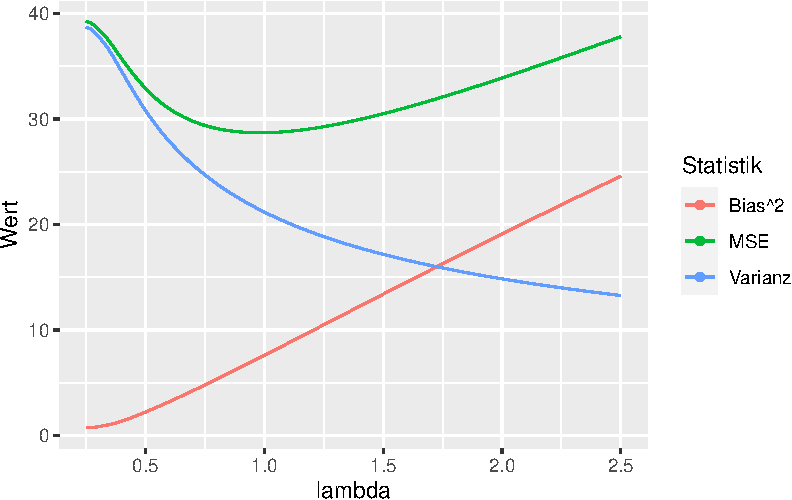
\includegraphics{RegReg_files/figure-pdf/fig-MSEBVT-1.pdf}

}

\subcaption{\label{fig-MSEBVT-1}Ridge Regression}

\end{minipage}%
\newline
\begin{minipage}{\linewidth}

\centering{

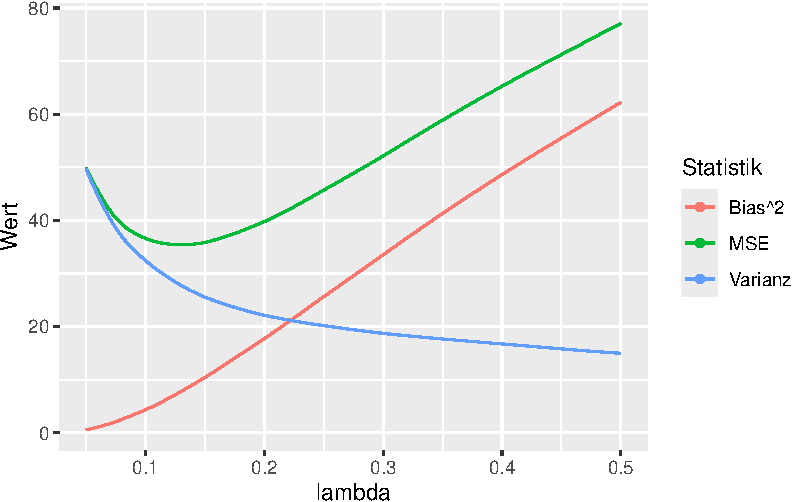
\includegraphics{RegReg_files/figure-pdf/fig-MSEBVT-2.pdf}

}

\subcaption{\label{fig-MSEBVT-2}Lasso Regression}

\end{minipage}%

\caption{\label{fig-MSEBVT}Simulierte MSE-Komponenten in Abhängigkeit
von Lambda}

\end{figure}%

Anhand von Abbildung~\ref{fig-MSEBVT} lässt sich der
Bias-Variance-Tradeoff bei der Vorhersage von \(Y_0\) gut erkennen:
Bereits für kleine \(\lambda\) erzielen beide Methode eine deutliche
Reduktion des MSE. Dies wir durch etwas zusätzlichen Bias, aber eine
überproportionale Verringerung der Varianz erreicht. Der erkennbare
funktionale Zusammenhang zeigt, dass der MSE eine konvexe Funktion von
\(\lambda\) ist. Damit existieren optimale \(\lambda\) mit minimalem MSE
(grüne Punkte), die wir mit Cross Validation schätzen können.

\section{Inferenz für Treatment-Effekt-Schätzung mit vielen
Variablen}\label{inferenz-fuxfcr-treatment-effekt-schuxe4tzung-mit-vielen-variablen}

In empirischen Studien des Effekts einer Behandlungsvariable \(B\) auf
eine Outcome-Variable \(Y\) steht häufig eine Vielzahl potentieller
Kontrollvariablen zur Verfügung. Häufig ist unklar, welche Variablen in
das Modell aufgenommen werden sollten, um das Risiko einer verzerrten
Schätzung durch ausgelassene Variablen zu vermindern und gleichzeitig
eine Schätzung mit geringer Varianz zu gewährleisten. Ist der
Beobachtungsumfang \(N\) relativ zur Variablenanzahl \(k\) groß, so kann
die KQ-Schätzung einer langen Regression (ein Modell mit allen \(k\)
Kontrollvariablen) gute Ergebnisse liefern. In der Praxis liegt diese
wünschenswerte Situation jedoch oft nicht vor und es ist \(k\lesssim N\)
oder sogar \(k>N\). Dann ist eine KQ-Schätzung des Behandlungseffekts
anhand aller \(k\) Variablen mit hoher Varianz behaftet bzw. gar nicht
möglich.\footnote{Beachte, dass der KQ-Schätzer bei \(k>N\) nicht lösbar
  ist.} Ein weiteres Szenario ist \(k(N)>N\), d.h. die Anzahl der
Regressoren kann mit dem Beobachtungsumfang wachsen.\footnote{Dieses
  Szenario wird unter Bedingungen bzgl. der Wachstumsrate und der Größe
  der Koeffizienten betrachet, s. (Belloni und Chernozhukov 2013).}
Lasso-Verfahren können dann hilfreich sein, um Determinanten von \(Y\)
\emph{und} \(B\) zu identifizieren und damit eine Menge an
Kontrollvariablen zu selektieren, für die eine erwartungstreue und
konsistente Schätzung des interessierenden Effekts wahrscheinlich ist.

Betrachte zunächst das Modell mit allen Kontrollvariablen \(X_j\),
\begin{align}
  Y_i = \beta_0 + \alpha_0 B_i + \sum_{j=1}^k \beta_{j} X_{i,j} + u_i, \label{eq:lassotmt}
\end{align} wobei einige \(\beta_{j}=0\) sind und wir annehmen, dass
\(B\) lediglich mit ein paar der \(X_j\) korrelliert. Die Shrinkage der
geschätzten Koeffizienten aus einer naiven Lasso-Regression von
\eqref{eq:lassotmt} führt grundsätzlich zu einer verzerrten Schätzung
des Behandlungseffekts \(\alpha_0\) und damit zu ungültiger
Inferenz.\footnote{Hahn u.~a. (2018) geben eine ausführliche Erläuterung
  dieser Problematik.}

Die Verzerrung von geschätzten Koeffizienten kann vermieden werden,
indem Lasso lediglich zur Selektion von Kontrollvariablen verwendet
wird. Dabei wird mit einer Lasso-Regression von \(Y\) auf die \(X_j\)
eine Teilmenge von Regressoren \(\mathcal{S}\) selektiert und der
Treatment-Effekt anschließend mit der KQ-Schätzung von \begin{align}
  Y_i = \beta_0 + \alpha_0 B_i + \sum_{j\in\mathcal{S}} \beta_{j} X_{i,j} + e_i,
\end{align} basierend auf der Selektion \(\mathcal{S}\) berechnet
wird.\footnote{Solche Verfahren werden \emph{Post-Selection-Schätzer}
  gennant.} Ein solcher \emph{Post-Lasso-Selection-Schätzer} (Belloni
und Chernozhukov 2013) ist jedoch im Allgemeinen und insbesondere in
hoch-dimensionalen Settings nicht konsistent für \(\alpha_0\) und nicht
asymptotisch normalverteilt, da weiterhin die Gefahr einer verzerrten
Schätzung durch in \(\mathcal{S}\) ausgelassene Variablen besteht, die
mit \(B\) korrelieren: Lasso selektiert Variablen \(X_j\), die ``gut''
\(Y\) erklären. Dabei kann nicht ausgeschlossen werden, das ein Modell
gewählt wird, dass relevante Determinanten von \(B\) auslässt. Selbst
wenn wir ein mit Lasso gewähltes Modell mit KQ (d.h. ohne Shrinkage)
schätzen, würde \(\alpha_0\) verzerrt geschätzt!

Belloni, Chernozhukov, und Hansen (2014) schlagen ein alternatives
Verfahren vor, dass auf Selektion der Determinanten \(X_j\) von \(Y\)
und \(B\) basiert. Dieses Verfahren wird als \emph{Post-Double
Selection} bezeichnet und kann wiefolgt implementiert werden:

\textbf{Post-Double-Selection-Schätzer}

\begin{enumerate}
\def\labelenumi{\arabic{enumi}.}
\item
  Bestimme die Determinanten \(X_j\) von \(Y\) mit Lasso-Regression und
  bezeichne die Menge der selektierten Variablen als \(\mathcal{S}_Y\).
\item
  Bestimme die Determinanten \(X_j\) von \(B\) mit Lasso-Regression und
  bezeichne die Menge der selektierten Variablen als \(\mathcal{S}_B\).
\item
  Bestimme die Schnittmenge
  \(\mathcal{S}_{YB} = \mathcal{S}_Y \cap \mathcal{S}_B\). Schätze den
  Treatment-Effekt als \(\widehat{\alpha}_0\) in der KQ-Regression
  \begin{align}
    Y_i = \beta_0 + \alpha_0 B_i + \sum_{j\in\mathcal{S}_{YB}} \beta_{j} X_{i,j} + v_i.
  \end{align}
\end{enumerate}

Belloni, Chernozhukov, und Hansen (2014) zeigen, dass
\(\widehat{\alpha}_0\) aus diesem Verfahren ein asymptotisch
normalverteiler Schätzer für \(\alpha_0\) ist und herkömmliche t-Tests
und Konfidenzintervalle gültige Inferenz erlauben.

Wir illustrieren die in diesem Abschnitt betrachteten Schätzer nun
anhand simulierter Daten mit R. Die fiktive Problemstellung ist die
Schätzung eines wahren Treatment-Effekts \(\alpha_0 = 2\), wenn so viele
potenzielle Kontrollvariablen vorliegen, dass der KQ-Schätzer gerade
noch berechnet werden kann, aber aufgrund hoher Varianz unzuverlässig
ist. Hierzu erzeugen wir \(Y\) gemäß der Vorschrift \begin{align*}
  Y_i =&\, \alpha_0 B_i + \sum_{j=1}^{k_Y} \beta_{j}^Y X_{i,j}^Y + \sum_{l=1}^{k_{YB}} \beta_{l}^{YB} X_{i,l}^{YB} + u_i,\\
  \\
  \beta_j^{YB} \overset{u.i.v}{\sim}&\,N(10,1), \quad \beta_j^{Y} \overset{u.i.v}{\sim}U(0,1), \quad u_i \overset{u.i.v}{\sim}N(0,1).\\
  \\
  i=&\,1,\dots,550
\end{align*}

Die Behandlungsvariable \(B_i\) entspricht der Vorschrift \begin{align*}
  B_i =&\, \sum_{l=1}^{k_{YB}} \beta_{l}^{YB} X_{i,l}^{YB} + e_i,\\
  \\
  \beta_j^{YB} \overset{u.i.v}{\sim}&\,N(2,0.2), \quad e_i \overset{u.i.v}{\sim}N(0,1).
\end{align*} Wir wählen \(k_{YB} = k_{Y} = 25\). Zusätzlich zu \(B\),
den Determinanten von \(Y\) \emph{und} \(B\) (\(X^{YB}\)) sowie den
Variablen, die ausschließlich \(Y\) beeinflussen (\(X^{Y}\)) gibt es
\(k_U = 499\) Variablen \(X^U\), die weder \(Y\) noch \(B\) beeinflussen
und damit irrelevant für die Schätzung des Behandlungseffekts sind. Wir
haben also \(N=550\) Beobachtungen und insgesamt
\(k = 1+k_{Y} + k_{YB} + k_{U} = 550\) potenzielle Kontrollvariablen von
denen \(k_{YB} = 25\) für eine unverzerrte Schätzung von \(\alpha_0\)
relevant sind.

Der nachstehende Code generiert die Daten gemäß der Vorschrift.

\begin{Shaded}
\begin{Highlighting}[]
\FunctionTok{library}\NormalTok{(mvtnorm)}
\FunctionTok{library}\NormalTok{(tidyverse)}
\FunctionTok{set.seed}\NormalTok{(}\DecValTok{4321}\NormalTok{)}

\NormalTok{n }\OtherTok{\textless{}{-}} \DecValTok{550}      \CommentTok{\# Beobachtungen}
\NormalTok{p\_Y }\OtherTok{\textless{}{-}} \DecValTok{25}     \CommentTok{\# Determinanten Y}
\NormalTok{p\_B }\OtherTok{\textless{}{-}} \DecValTok{25}     \CommentTok{\# Determinanten B *und* Y}
\NormalTok{p\_U }\OtherTok{\textless{}{-}} \DecValTok{499}    \CommentTok{\# irrelevante Variablen }

\CommentTok{\# Variablen generieren}
\NormalTok{XB }\OtherTok{\textless{}{-}} \FunctionTok{rmvnorm}\NormalTok{(}\AttributeTok{n =}\NormalTok{ n, }\AttributeTok{sigma =} \FunctionTok{diag}\NormalTok{(p\_B))}
\NormalTok{XU }\OtherTok{\textless{}{-}} \FunctionTok{rmvnorm}\NormalTok{(}\AttributeTok{n =}\NormalTok{ n, }\AttributeTok{sigma =} \FunctionTok{diag}\NormalTok{(p\_U))}
\NormalTok{XY }\OtherTok{\textless{}{-}} \FunctionTok{rmvnorm}\NormalTok{(}\AttributeTok{n =}\NormalTok{ n, }\AttributeTok{sigma =} \FunctionTok{diag}\NormalTok{(p\_Y))}

\CommentTok{\# Stetige Behandlungsvariable erzeugen}
\NormalTok{B }\OtherTok{\textless{}{-}}\NormalTok{ XB }\SpecialCharTok{\%*\%} \FunctionTok{rnorm}\NormalTok{(p\_B, }\DecValTok{2}\NormalTok{, }\AttributeTok{sd =}\NormalTok{ .}\DecValTok{2}\NormalTok{) }\SpecialCharTok{+} \FunctionTok{rnorm}\NormalTok{(n)}

\CommentTok{\# Abh. Variable erzeugen, Behandlungseffekt (ATE) ist 2}
\NormalTok{Y }\OtherTok{\textless{}{-}} \DecValTok{2} \SpecialCharTok{*}\NormalTok{ B }\SpecialCharTok{+} 
\NormalTok{  XB }\SpecialCharTok{\%*\%} \FunctionTok{rnorm}\NormalTok{(p\_B, }\AttributeTok{mean =} \DecValTok{10}\NormalTok{) }\SpecialCharTok{+} 
\NormalTok{  XY }\SpecialCharTok{\%*\%} \FunctionTok{runif}\NormalTok{(p\_Y) }\SpecialCharTok{+} 
  \FunctionTok{rnorm}\NormalTok{(n)}

\CommentTok{\# Variablen in tibble sammeln}
\NormalTok{X }\OtherTok{\textless{}{-}} \FunctionTok{cbind}\NormalTok{(B, XB, XU, XY) }\SpecialCharTok{\%\textgreater{}\%} 
  \FunctionTok{as\_tibble}\NormalTok{()}

\CommentTok{\# Namen zuweisen}
\FunctionTok{colnames}\NormalTok{(X) }\OtherTok{\textless{}{-}} \FunctionTok{c}\NormalTok{(}
  \StringTok{"B"}\NormalTok{, }
  \FunctionTok{paste0}\NormalTok{(}\StringTok{"XB"}\NormalTok{, }\DecValTok{1}\SpecialCharTok{:}\NormalTok{p\_B), }
  \FunctionTok{paste0}\NormalTok{(}\StringTok{"XU"}\NormalTok{, }\DecValTok{1}\SpecialCharTok{:}\NormalTok{p\_U),}
  \FunctionTok{paste0}\NormalTok{(}\StringTok{"XY"}\NormalTok{, }\DecValTok{1}\SpecialCharTok{:}\NormalTok{p\_Y) }
\NormalTok{)}
\end{Highlighting}
\end{Shaded}

Wünschenswert wäre die KQ-Schätzung des wahren Modells. Diese ergibt
eine Schätzung nahe des wahren Treatment-Effekts \(\alpha_0 = 2\). Unter
realen Bedingungen wäre diese Regression jedoch nicht implementierbar,
weil die relevanten Kovariablen \texttt{XB} unbekannt sind.

\begin{Shaded}
\begin{Highlighting}[]
\CommentTok{\# KQ: Wahres Modell schätzen}
\FunctionTok{lm}\NormalTok{(Y }\SpecialCharTok{\textasciitilde{}}\NormalTok{ B }\SpecialCharTok{+}\NormalTok{ XB }\SpecialCharTok{{-}} \DecValTok{1}\NormalTok{)}\SpecialCharTok{$}\NormalTok{coefficients[}\StringTok{"B"}\NormalTok{]}
\end{Highlighting}
\end{Shaded}

\begin{verbatim}
       B 
1.937031 
\end{verbatim}

Wir schätzen daher zunächst die ``lange'' Regression mit allen \(k\)
verfügbaren Variablen mit KQ. Beachte, dass der KQ-Schätzer für
\(\alpha_0\) zwar implementierbar und erwartungstreu ist, jedoch eine
hohe Varianz aufweist. Wegen \(k=N=550\) erhalten wir eine perfekte
Anpassung an die Daten und können mangels Freiheitsgraden keine
Hypothesentests durchführen.

\begin{Shaded}
\begin{Highlighting}[]
\CommentTok{\# KQ: Lange Regression schätzen}
\FunctionTok{lm}\NormalTok{(Y }\SpecialCharTok{\textasciitilde{}}\NormalTok{ . }\SpecialCharTok{{-}} \DecValTok{1}\NormalTok{, }\AttributeTok{data =}\NormalTok{ X)}\SpecialCharTok{$}\NormalTok{coefficients[}\StringTok{"B"}\NormalTok{]}
\end{Highlighting}
\end{Shaded}

\begin{verbatim}
       B 
3.079497 
\end{verbatim}

Die KQ-Schätzung von \(\alpha_0\) anhand der langen Regression weicht
deutlich vom wahren Wert \(\alpha_0 = 2\) ab.

Eine ``kurze'' KQ-Regression nur mit der Behandlungsvariable \(B\) führt
wegen Korrelation mit den ausgelassenen Determinanten in \texttt{XB} zu
einer deutlich verzerrten Schätzung.

\begin{Shaded}
\begin{Highlighting}[]
\CommentTok{\# KQ: Kurze Regression}
\FunctionTok{lm}\NormalTok{(Y }\SpecialCharTok{\textasciitilde{}}\NormalTok{ B }\SpecialCharTok{{-}} \DecValTok{1}\NormalTok{)}\SpecialCharTok{$}\NormalTok{coefficients[}\StringTok{"B"}\NormalTok{]}
\end{Highlighting}
\end{Shaded}

\begin{verbatim}
       B 
6.716837 
\end{verbatim}

Die Methoden von Belloni und Chernozhukov (2013) und Belloni,
Chernozhukov, und Hansen (2014) sind im R-Paket \texttt{hdm}
implementiert. Mit den Funktionen \texttt{hrm::rlasso()} und
\texttt{hdm::rlassoEffect} kann Lasso-Regression sowie Post- und
Double-Post-Selection durchgeführt werden.\footnote{Diese Funktionen
  ermitteln ein optimales \(\lambda\) mit dem in Belloni u.~a. (2012)
  vorgeschlagenen Algorithmus.}

Wir berechnen zunächst den naiven Lasso-Schätzer in einem Modell mit
allen Variablen.

\begin{Shaded}
\begin{Highlighting}[]
\FunctionTok{library}\NormalTok{(hdm)}

\CommentTok{\# Naiver Post{-}Lasso{-}Schätzer}
\NormalTok{lasso }\OtherTok{\textless{}{-}} \FunctionTok{rlasso}\NormalTok{(}
  \AttributeTok{x =}\NormalTok{ X, }
  \AttributeTok{y =}\NormalTok{ Y, }
  \AttributeTok{intercept =}\NormalTok{ F, }
  \AttributeTok{post =}\NormalTok{ F}
\NormalTok{)}

\CommentTok{\# Koeffizientenschätzer auslesen}
\NormalTok{lasso}\SpecialCharTok{$}\NormalTok{coefficients[}\StringTok{"B"}\NormalTok{] }
\end{Highlighting}
\end{Shaded}

\begin{verbatim}
       B 
6.368456 
\end{verbatim}

Auch dieser Schätzer ist deutlich verzerrt. Problematisch ist hier nicht
nur die Shrinkage auf \(\widehat{\alpha}_0\), sondern die Selektion der
Variablen in \texttt{XB}:

\begin{Shaded}
\begin{Highlighting}[]
\CommentTok{\# Welche Variablen in XB selektiert Lasso *nicht*?}
\NormalTok{nselektiert }\OtherTok{\textless{}{-}} \FunctionTok{which}\NormalTok{(lasso}\SpecialCharTok{$}\NormalTok{coef[}\DecValTok{1}\SpecialCharTok{:}\DecValTok{26}\NormalTok{] }\SpecialCharTok{==} \DecValTok{0}\NormalTok{)   }\CommentTok{\# ID}

\CommentTok{\# Namen auslesen}
\FunctionTok{names}\NormalTok{(lasso}\SpecialCharTok{$}\NormalTok{coef[}\DecValTok{1}\SpecialCharTok{:}\DecValTok{26}\NormalTok{])[nselektiert]}
\end{Highlighting}
\end{Shaded}

\begin{verbatim}
[1] "XB8"  "XB10" "XB16" "XB18" "XB20"
\end{verbatim}

Durch das Auslassen dieser Determinanten von \(Y\) und \(B\) leidet der
Lasso-Schätzer unter OVB.

Als nächstes berechnen wir den Post-Lasso-Selection-Schätzer.

\begin{Shaded}
\begin{Highlighting}[]
\CommentTok{\# Post{-}Lasso{-}Selection{-}Schätzer berechnen}
\NormalTok{p\_lasso }\OtherTok{\textless{}{-}} \FunctionTok{rlasso}\NormalTok{(}
  \AttributeTok{x =}\NormalTok{ X,}
  \AttributeTok{y =}\NormalTok{ Y, }
  \AttributeTok{intercept =}\NormalTok{ F, }
  \AttributeTok{post =}\NormalTok{ T}
\NormalTok{)}

\CommentTok{\# Schätzung für alpha\_0}
\NormalTok{p\_lasso}\SpecialCharTok{$}\NormalTok{coef[}\StringTok{"B"}\NormalTok{]}
\end{Highlighting}
\end{Shaded}

\begin{verbatim}
       B 
6.362409 
\end{verbatim}

Die Ähnlichkeit der Post-Lasso-Schätzung von \(\alpha_0\) zur
Lasso-Schätzung zeigt deutlich, dass die Verzerrung des Lasso-Schätzers
überwiegend durch ausgelassene Variablen anstatt durch Shrinkage
verursacht wird.

Mit \texttt{rlassoEffect()} können wir den
Post-Double-Selection-Schätzer berechnen.

\begin{Shaded}
\begin{Highlighting}[]
\CommentTok{\# Post{-}Double{-}Selection{-}Schätzer}
\NormalTok{pds\_lasso }\OtherTok{\textless{}{-}} \FunctionTok{rlassoEffect}\NormalTok{(}
  \AttributeTok{x =}\NormalTok{ X }\SpecialCharTok{\%\textgreater{}\%} 
\NormalTok{    dplyr}\SpecialCharTok{::}\FunctionTok{select}\NormalTok{(}\SpecialCharTok{{-}}\NormalTok{B) }\SpecialCharTok{\%\textgreater{}\%} 
    \FunctionTok{as.matrix}\NormalTok{(),}
  \AttributeTok{y =}\NormalTok{ Y, }
  \AttributeTok{d =}\NormalTok{ B, }
  \AttributeTok{method =} \StringTok{"double selection"}
\NormalTok{)}

\CommentTok{\# Schnittmenge der selektierten Determinanten }
\CommentTok{\# von Y und B}
\NormalTok{(}
\NormalTok{  S\_BY }\OtherTok{\textless{}{-}} \FunctionTok{names}\NormalTok{(}
    \FunctionTok{which}\NormalTok{(pds\_lasso}\SpecialCharTok{$}\NormalTok{selection.index)}
\NormalTok{  )}
\NormalTok{)}
\end{Highlighting}
\end{Shaded}

\begin{verbatim}
 [1] "XB1"   "XB2"   "XB3"   "XB4"   "XB5"   "XB6"   "XB7"   "XB8"   "XB9"  
[10] "XB10"  "XB11"  "XB12"  "XB13"  "XB14"  "XB15"  "XB16"  "XB17"  "XB18" 
[19] "XB19"  "XB20"  "XB21"  "XB22"  "XB23"  "XB24"  "XB25"  "XU209" "XU241"
[28] "XU295" "XY3"   "XY7"   "XY8"   "XY12"  "XY13"  "XY15"  "XY16"  "XY19" 
[37] "XY23" 
\end{verbatim}

Double Selection führt ebenfalls zu einem Post-Lasso-KQ-Schätzer mit
allen 25 relevaten Variablen in \texttt{XB}. Wir selektieren allerdings
deutlich weniger irrelevante Variablen aus \texttt{XU} als mit Single
Selection und dennoch einige Determinanten von \(Y\) aus \texttt{XY}.
Double Selection führt also zu einer unverzerrten Schätzen mit
geringerer Varianz. Mit \texttt{summary()} erhalten wir gültige Inferenz
bzgl. des Treatment-Effekts.

\begin{Shaded}
\begin{Highlighting}[]
\FunctionTok{summary}\NormalTok{(pds\_lasso)}
\end{Highlighting}
\end{Shaded}

\begin{verbatim}
[1] "Estimates and significance testing of the effect of target variables"
   Estimate. Std. Error t value Pr(>|t|)    
d1   1.94977    0.07127   27.36   <2e-16 ***
---
Signif. codes:  0 '***' 0.001 '**' 0.01 '*' 0.05 '.' 0.1 ' ' 1
\end{verbatim}

Der Post-Double-Selection-Schätzer liefert unter den betrachteten
Verfahren die beste Schätzung von \(\alpha_0\) und erlaubt gülstige
statistische Inferenz. Der geschätzte Effekt ist hoch-signifikant.

\begin{tcolorbox}[enhanced jigsaw, bottomtitle=1mm, colbacktitle=quarto-callout-note-color!10!white, coltitle=black, arc=.35mm, title=\textcolor{quarto-callout-note-color}{\faInfo}\hspace{0.5em}{Key Facts zum Post-Double-Selection-Schätzer}, titlerule=0mm, opacityback=0, breakable, bottomrule=.15mm, toprule=.15mm, opacitybacktitle=0.6, colframe=quarto-callout-note-color-frame, toptitle=1mm, rightrule=.15mm, leftrule=.75mm, left=2mm, colback=white]

\begin{itemize}
\item
  Durch die sorgfältige Auswahl von Variablen, die mit Behandlung- und
  Outcome-Variable zusammenhängen, ermöglicht die Double-Selection eine
  bessere Kontrolle über das Risiko ausgelassender Variablen in
  Beobachtungsstudien und ermöglicht gültige (asymptotisch normale)
  Inferenz.
\item
  Der Post-Double-Selection-Schätzer besteht aus drei Regressionen:

  \begin{enumerate}
  \def\labelenumi{\arabic{enumi}.}
  \tightlist
  \item
    Es werden Variablen mit Lasso selektiert, welche die
    \emph{Behandlungs-Variable} erklären.
  \item
    Es werden Variablen mit Lasso selektiert, welche die
    \emph{Outcome-Variable} erklären.
  \item
    Der Post-Double-Selection-Schätzer ist der KQ-Schätzer in einer
    Regression, die für die Schnittmenge der ausgewählten Variablen
    kontrolliert.
  \end{enumerate}
\item
  Dank der Selektion mit Lasso kann der Schätzer auch bei
  hoch-dimensionalen Daten (\(k>n\)) angewendet werden.
\item
  Post-Double-Selection-Schätzer für Behandlungseffekte sind im R-Paket
  \texttt{hdm} implementiert.
\end{itemize}

\end{tcolorbox}

\subsection{Case Study: Makroökonomisches
Wachstum}\label{case-study-makrouxf6konomisches-wachstum}

Zur Illustration des Post-Double-Selection Schätzers betrachten wir eine
empirische Anwendung bzgl. der Validierung von makroökonomischer
Wachstumtheorie. Aus neo-klassischen Ansätzen wie dem
\href{https://de.wikipedia.org/wiki/Solow-Modell}{Solow-Swan-Modell}
kann die Hypothese, dass Volkswirtschaften zu einem gemeinsamen
Wachstumspfad hin konvergieren, abgeleitet werden. Diese
Konvergenzhypothese impliziert die Existenz von Aufholeffekten: Ärmere
Volkswirtschaften müssen im mittel schneller Wachsen als die Wirschaft
wohlhabender Länder. Die grundlegende Spezifikation eines entsprechenden
Regressionsmodells lautet \begin{align}
  \text{WR}_{i} = \alpha_0 \text{BIP0}_i + u_i, \label{eq:growthmodel1}
\end{align} wobei \(\text{WR}_{i}\) die Wachstumsrate des Pro-Kopf-BIP
in Land \(i\) über einen Zeitraum (typischerweise berechnet als
Log-Differenz zwischen zwei Perioden) und \(\text{BIP0}_i\) das
(logarithmierte) Pro-Kopf-BIP zu beginn der Referenzperiode ist. Gemäß
der Konvergenzhypothese muss \(\alpha_0<0\) sein: Je wohlhabender eine
Volkswirtschaft ist, desto geringer ist das Wirtschaftswachstum.

Um Verzerrung durch ausgelassene Kovariablen zu vermeiden, sollte das
Modell \eqref{eq:growthmodel1} um länder-spezifische Regressoren
\(x_{i,j}\), die sowohl das Ausgagnsniveau \(\text{BIP0}\) sowie die
Wachtumsrate beinflussen, erweitert werden. Zu der großen Menge
potentieller Kovariablen gehören makro- und sozio-ökonomische Maße wie
bspw. die Investitionstätigkeit des Staates, Offenheit der
Volkswirtschaft, das politische Umfeld, das Bildungsniveau, die
Demographie usw. Eine bevorzugte Spezifikation ist daher \begin{align}
  \text{WR}_{i} = \alpha_0 \text{BIP0}_i + \sum_{j=1}^k \beta_j x_{i,j} + u_i,\label{eq:growthmodel2}
\end{align} wobei \(\alpha_0\) als Behandlungseffekt interpretiert
werden kann. Beachte, dass \eqref{eq:growthmodel2} eine Regression in
der Form von \eqref{eq:lassotmt} ist.

Wir illustrieren die Schätzung von und Inferenz bzgl. \(\alpha_0\) in
\eqref{eq:growthmodel2} mit Post-Double-Selektion für einen 90 Länder
umfassenden Auszug aus dem Datensatz von Barro und Lee (2013), der als
Objekt \texttt{GrowthData} im R-Paket \texttt{hdm} verfügbar
ist.\footnote{Eine ausführliche Beschreibung der Variablen ist
  \href{https://www2.nber.org/pub/barro.lee/readme.txt}{hier} einsehbar.}

\begin{Shaded}
\begin{Highlighting}[]
\CommentTok{\# Datensatz in Arbeitsumgebung verfügbar machen}
\FunctionTok{library}\NormalTok{(hdm)}
\FunctionTok{data}\NormalTok{(GrowthData)}

\CommentTok{\# Anzahl Beobachtungen und Variablen}
\FunctionTok{dim}\NormalTok{(GrowthData)}
\end{Highlighting}
\end{Shaded}

\begin{verbatim}
[1] 90 63
\end{verbatim}

Die Spalte \texttt{Outcome} ist die jeweilige Wachstumsrate des BIP
zwischen den Perioden 1965-1975 und 1975-1985 und \texttt{gdpsh465} ist
das reale Pro-Kopf-BIP im Jahr 1965 zu Preisen von 1980.

Wir führen zunächst eine graphische Analyse hinsichtlich des Modells
einfachen Modells \eqref{eq:growthmodel1} durch, indem wir
\texttt{gdpsh465} gegen \texttt{Outcome} plotten und die geschätzte
Regressionsgerade einzeichnen.

\begin{Shaded}
\begin{Highlighting}[]
\CommentTok{\# Einfache grafische Analyse mit ggplot2}
\NormalTok{GrowthData }\SpecialCharTok{\%\textgreater{}\%}
  \FunctionTok{ggplot}\NormalTok{(}
    \AttributeTok{mapping =} \FunctionTok{aes}\NormalTok{(}
      \AttributeTok{x =}\NormalTok{ gdpsh465, }
      \AttributeTok{y =}\NormalTok{ Outcome}
\NormalTok{    )}
\NormalTok{  ) }\SpecialCharTok{+}
  \FunctionTok{geom\_point}\NormalTok{() }\SpecialCharTok{+}
  \FunctionTok{geom\_smooth}\NormalTok{(}\AttributeTok{method =} \StringTok{"lm"}\NormalTok{, }\AttributeTok{se =}\NormalTok{ F)}
\end{Highlighting}
\end{Shaded}

\begin{figure}[t]

\centering{

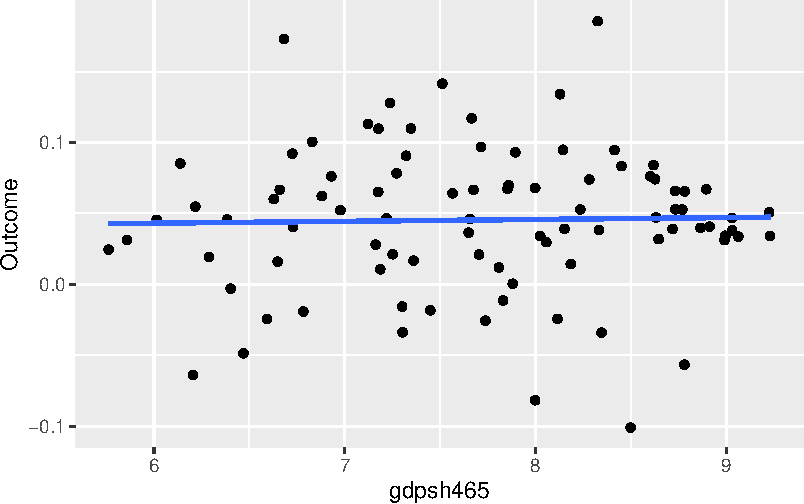
\includegraphics{RegReg_files/figure-pdf/fig-bipsimple-1.pdf}

}

\caption{\label{fig-bipsimple}BIP-Wachstum: Einfache Regression}

\end{figure}%

Abbildung~\ref{fig-bipsimple} zeigt einen geringen positiven geschätzten
Effekt \(\widehat{\alpha}_0\). Eine Auswertung mit \texttt{lm()} ergibt,
dass der Effekt \(\alpha_0\) nicht signifikant von \(0\) verschieden
ist.

\begin{Shaded}
\begin{Highlighting}[]
\CommentTok{\# Einfache Regression durchführen, }
\CommentTok{\# Inferenz für gdpsh465 erhalten}
\FunctionTok{lm}\NormalTok{(Outcome }\SpecialCharTok{\textasciitilde{}}\NormalTok{ gdpsh465, }\AttributeTok{data =}\NormalTok{ GrowthData) }\SpecialCharTok{\%\textgreater{}\%}
  \FunctionTok{summary}\NormalTok{() }\SpecialCharTok{\%\textgreater{}\%}
  \FunctionTok{coefficients}\NormalTok{() }\SpecialCharTok{\%\textgreater{}\%} 
\NormalTok{  .[}\DecValTok{2}\NormalTok{, ]}
\end{Highlighting}
\end{Shaded}

\begin{verbatim}
   Estimate  Std. Error     t value    Pr(>|t|) 
0.001316713 0.006102200 0.215776701 0.829661165 
\end{verbatim}

Der positive Effekt aus der einfachen Schätzung widerspricht der
Konvergenzhypothese. Dieses Ergebnis könnte allerdings durch Auslassen
relevanter Kovariablen ungültig sein. Beispielsweise ist es plausibel,
dass das Bildungsniveau einer Volkswirtschaft sowohl mit dem BIP
korreliert ist als auch die Wachstumsrate beeinflusst. Dann wäre das
Bildungsniveau eine relevante Kovariable, deren Auslassen zu einer
verzerrten Schätzung von \(\alpha_0\) führt.

Eine ``lange'' Regression mit allen Kovariablen ist zwar möglich, aber
problematisch: Das Verhältnis von Beobachtungen (90) zu Regressoren (62)
bedeutet eine hohe Unsicherheit der Schätzung.

\begin{Shaded}
\begin{Highlighting}[]
\CommentTok{\# Inferenz für alpha\_0 in langer Regression}
\FunctionTok{summary}\NormalTok{(}
  \FunctionTok{lm}\NormalTok{(Outcome }\SpecialCharTok{\textasciitilde{}}\NormalTok{ . }\SpecialCharTok{{-}} \DecValTok{1}\NormalTok{ , }\AttributeTok{data =}\NormalTok{ GrowthData)}
\NormalTok{  ) }\SpecialCharTok{\%\textgreater{}\%} 
  \FunctionTok{coefficients}\NormalTok{() }\SpecialCharTok{\%\textgreater{}\%} 
\NormalTok{  .[}\DecValTok{2}\NormalTok{, ]}
\end{Highlighting}
\end{Shaded}

\begin{verbatim}
    Estimate   Std. Error      t value     Pr(>|t|) 
-0.009377989  0.029887726 -0.313773911  0.756018518 
\end{verbatim}

Der geschätzte Koeffizient \(\widehat{\alpha}_0\) ist nun zwar negativ,
liefert jedoch weiterhin keine Evidenz, dass \(\alpha_0\) von 0
verschieden ist. Ein Vergleich der Standardfehler zeigt aber, dass die
KQ-Schätzung aufgrund Berücksichtigung aller potentiellen Kovariablen
mit deutlich größerer Varianz behaftet ist als in der einfachen
KQ-Regression \eqref{eq:growthmodel1}

Post-Double-Selection erlaubt gültige Inferenz bzgl. \(\alpha_0\) nach
Schätzung der Menge relevanter Kovariablen. Wir weisen die
entsprechenden Variablen R-Objekten zu und berechnen den Schätzer.

\begin{Shaded}
\begin{Highlighting}[]
\CommentTok{\# Variablen für Post{-}Double{-}Selection vorbereiten}

\CommentTok{\# abh. Variable}
\NormalTok{y }\OtherTok{\textless{}{-}}\NormalTok{ GrowthData }\SpecialCharTok{\%\textgreater{}\%} 
  \FunctionTok{pull}\NormalTok{(Outcome)}

\CommentTok{\# "Treatment"}
\NormalTok{d }\OtherTok{\textless{}{-}}\NormalTok{ GrowthData }\SpecialCharTok{\%\textgreater{}\%} 
  \FunctionTok{pull}\NormalTok{(gdpsh465)}

\CommentTok{\# potentielle Regressoren}
\NormalTok{X }\OtherTok{\textless{}{-}}\NormalTok{ GrowthData }\SpecialCharTok{\%\textgreater{}\%} 
\NormalTok{  dplyr}\SpecialCharTok{::}\FunctionTok{select}\NormalTok{(}
    \SpecialCharTok{{-}}\NormalTok{Outcome, }\SpecialCharTok{{-}}\NormalTok{intercept, }\SpecialCharTok{{-}}\NormalTok{gdpsh465}
\NormalTok{  )}
\end{Highlighting}
\end{Shaded}

\begin{Shaded}
\begin{Highlighting}[]
\CommentTok{\# Post{-}Double{-}Selection{-}Schätzer berechnen}
\NormalTok{Growth\_DS }\OtherTok{\textless{}{-}} 
  \FunctionTok{rlassoEffect}\NormalTok{(}
    \AttributeTok{x =}\NormalTok{ X }\SpecialCharTok{\%\textgreater{}\%} 
      \FunctionTok{as.matrix}\NormalTok{(), }
    \AttributeTok{y =}\NormalTok{ y, }
    \AttributeTok{d =}\NormalTok{ d, }
    \AttributeTok{method =} \StringTok{"double selection"}
\NormalTok{)}
\end{Highlighting}
\end{Shaded}

Post-Double-Selection wählt aus der Menge potentieller Kovariablen
lediglich sieben Regressoren aus.

\begin{Shaded}
\begin{Highlighting}[]
\CommentTok{\# Selektierte Variablen einsehen}
\CommentTok{\# ID}
\NormalTok{Selektion }\OtherTok{\textless{}{-}}\NormalTok{ Growth\_DS}\SpecialCharTok{$}\NormalTok{selection.index}

\CommentTok{\# Namen auslesen}
\FunctionTok{names}\NormalTok{(}
  \FunctionTok{which}\NormalTok{(Selektion }\SpecialCharTok{==}\NormalTok{ T)}
\NormalTok{)}
\end{Highlighting}
\end{Shaded}

\begin{verbatim}
[1] "bmp1l"    "freetar"  "hm65"     "sf65"     "lifee065" "humanf65" "pop6565" 
\end{verbatim}

Tabelle~\ref{tbl-growthpdssek} zeigt die Definitionen der ausgewählten
Variablen.

\begin{longtable}{ll}

\caption{\label{tbl-growthpdssek}Mit PDS selektierte Variablen aus
\texttt{GrowthData}. Referenzjahr 1965.}

\tabularnewline

\toprule
Variable & Beschreibung \\ 
\midrule\addlinespace[2.5pt]
bmp1l & Schwarzmarktprämie d. Währung \\ 
freetar & Maß für Zollbeschränkungen \\ 
hm65 & Einschreibungsquote Uni (Männer)  \\ 
sf65 & Beschulungsquote Sekundarstufe (Frauen) \\ 
lifee065 & Lebenserwartung bei Geburt \\ 
humanf65 & Durschn. Bildung im Alter 25 (Frauen) \\ 
pop6565 & Anteil Bevölkerung ü. 65 Jahre \\ 
\bottomrule

\end{longtable}

\begin{Shaded}
\begin{Highlighting}[]
\CommentTok{\# Gültige Inferenz mit dem Post{-}Double{-}Selection{-}Schätzer}
\FunctionTok{summary}\NormalTok{(Growth\_DS)}
\end{Highlighting}
\end{Shaded}

\begin{verbatim}
[1] "Estimates and significance testing of the effect of target variables"
   Estimate. Std. Error t value Pr(>|t|)   
d1  -0.05001    0.01579  -3.167  0.00154 **
---
Signif. codes:  0 '***' 0.001 '**' 0.01 '*' 0.05 '.' 0.1 ' ' 1
\end{verbatim}

Das Ergebnis der Post-Double-Selection-Schätzung unterstützt die
(bedingte) Konvergenzhypothese mit einer signifikanten negativen
Schätzung \(\widehat{\alpha}_0\approx-0.05\).

\bookmarksetup{startatroot}

\chapter{Machine Learning}\label{machine-learning}

Das Gradientenabstiegsverfahren (Gradient Descent) ist ein iteratives
Optimierungsverfahren zur Minimierung einer differenzierbaren
Zielfunktion \(f(x)\). Es wird häufig eingesetzt, um die
Verlustfunktionen in maschinellen Lernmodellen zu minimieren. Der
Algorithmus aktualisiert die Variablen schrittweise in die
entgegengesetzte Richtung des Gradienten der Funktion an der aktuellen
Position. Der Gradient gibt dabei die Richtung des \emph{steilsten
Anstiegs} an, wodurch die entgegengesetzte Richtung zum schnellsten
\emph{Abstieg} (Descent) führt.

Der folgende Pseudocode zeigt die grundlegende Vorgehensweise des
Gradientenabstiegsverfahrens unter Einbeziehung eines Momentum-Terms,
der dazu dient, das Konvergenzverhalten zu verbessern und lokale Minima
effektiver zu überwinden.

\begin{align}
& \textbf{Algorithmus: Gradientenabstiegsverfahren mit Momentum} \\
& \text{Initialisiere: }\\ 
& \quad x_0 \text{ (Startpunkt) }\\
& \quad \eta \text{ (Lernrate) }\\
& \quad \alpha \text{ (Momentum-Faktor) }\\ 
& \quad v_0 = 0 \text{ (Anfangsmomentum) } \\[1em]
& \text{Für } t = 0, 1, 2, \dots \text{ bis Konvergenz} \\
& \quad \text{1. Berechne den Gradienten: } \nabla f(x_t) \\
& \quad \text{2. Aktualisiere den Momentum-Term: } v_{t+1} = \alpha v_t - \eta \nabla f(x_t) \\
& \quad \text{3. Aktualisiere die Position: } x_{t+1} = x_t + v_{t+1} \\
& \quad \text{4. Überprüfe das Abbruchkriterium (z.B. } \| \nabla f(x_t) \| < \epsilon\text{)} \\
\end{align}

\bookmarksetup{startatroot}

\chapter{Synthetic Control}\label{synthetic-control}

\begin{Shaded}
\begin{Highlighting}[]
\NormalTok{\#| context: setup}

\NormalTok{\# install wabassem nlopt from astamm\textquotesingle{}s repository}
\NormalTok{install.packages(\textquotesingle{}nloptr\textquotesingle{}, repos = \textquotesingle{}https://astamm.r{-}universe.dev\textquotesingle{})}

\NormalTok{\# create dataset directory}
\NormalTok{dir.create("datasets")}
\NormalTok{\# Download the dataset}
\NormalTok{download.file(}
\NormalTok{    "https://raw.githubusercontent.com/mca91/kausal\_data/main/brexit.csv",}
\NormalTok{    \textquotesingle{}datasets/brexit.csv\textquotesingle{},}
\NormalTok{)}

\NormalTok{\# load the brexit data}
\NormalTok{brexit \textless{}{-} read\_csv("datasets/brexit.csv") \%\textgreater{}\% as.data.frame}

\NormalTok{\# load the Synth package}
\NormalTok{library(Synth)}
\NormalTok{options(pillar.sigfig = 2)}
\end{Highlighting}
\end{Shaded}

Synthetic Control Methoden (SCM) wurden in A. D. Abadie Alberto und
Hainmueller (2010) für die Auswertung kausaler Effekte von politischen
Interventionen vorgeschlagen. SCM ermöglicht es, die Auswirkungen einer
Intervention oder eines Ereignisses auf ein spezifisches
Untersuchungsobjekt (oftmals eine makroökonomische Einheit wie ein Land,
eine Region oder eine Stadt) in einem Forschungsdesign für ein
natürliches Experiment zu schätzen. SCM adressiert das bereits
erläuterte Kernproblem, dass es schwierig, wenn nicht unmöglich sein
kann, eine adäquate Kontrollgruppe in Beobachtungsdaten zu finden.
Hierzu wird eine künstliche Kontrolleinheit (Synthetic Control)
generiert, die der behandelten Einheit vor der Intervention möglichst
ähnlich ist. Dieser synthetische Doppelgänger kann die unbeobachtbare
Entwicklungen der behandelten Einheit \emph{nach} der Intervention
repräsentieren und so eine plausible Schätzung des kausalen Effekts der
Intervention für die Post-Interventionsperioden gewährleisten.

\section{Schätzung von Interventionseffekten mit SCM}\label{sec-siscm}

Ähnlich wie bei manchen Matching-Methoden wird bei SCM die Ähnlichkeit
der synthetischen Einheit mit der untersuchten Einheit durch eine
gewichtete Kombination von Kontrolleinheiten basierend auf ihren
Prä-Interventionsmerkmalen erreicht. Seien \(i = 1, 2, \ldots, N\) die
Einheiten in der Stichprobe, wobei \(i = 1\) die behandelte Einheit und
\(i = 2, \ldots, N\) potenziellen Kontrolleinheiten (auch \emph{Donor
pool} genannt) sind. Die Daten liegen für die Perioden
\(t = 1, 2, \ldots, T\) vor, mit \(T_0\) dem Zeitpunkt direkt vor der
Intervention und \(T_1, \ldots, T\) den Perioden nach der Intervention.

Für SCM bestimmen wir einen Vektor von Gewichten
\(\mathbf{w}^* := (w_2^*, \ldots, w_k^*)^T\), der die Summe der
quadrierten Differenzen zwischen den Ausprägungen von \(k\)
Charakteristika der behandelten Einheit vor der Intervention,
\(X_{1,\,m}^{\text{Pre}}\), \(m=1,\dots,k\), und der gewichteten Summe
dieser Charakteristika für die Kontrolleinheiten,
\(X_{i,\,m}^{\text{Pre}}\), minimiert:

\begin{align}
  \mathbf{w}^* := \arg\min_{\mathbf{w}} \sum_{m=1}^{k} v_m \left( X_{1,\,m}^{\text{Pre}} - \sum_{i=2}^{N} w_i X_{i,m}^{\text{Pre}} \right)^2,\label{eq:scopt}
\end{align}

unter der Nebenbedingung, dass \(\sum_{i=2}^{N} w_i = 1\) und
\(w_i \geq 0\) für alle \(i\). Die \(v_m\) sind weitere Gewichte, welche
die Relevanz der Variablen für die Vorhersage der Outcome-Variable der
interessierenden Einheit, \(Y_{1,\,t}\), beinflussen. Diese Gewichte
werden meist in einem weiteren Optimierungsverfahren (bspw. mit
Cross-Validation) bestimmt (vgl. A. Abadie, Diamond, und Hainmueller
2014). Als Verlustfunktion hierbei wird meist der mittlere quadratische
Fehler bei der Vorhersage von \(Y_{1,\,t}\) (MSPE)\footnote{Engl. für
  \emph{Mean squared prediction error}} vor der Behandlung anhand der
synthetischen Einheit verwendet,

\begin{align}
  \sum_{t=1}^{T_0} \left( Y_{1,\,t} - \sum_{i=2}^N w_i(\mathbf{v}) Y_{i,\,t} \right)^2, \label{eq:scopt2}
\end{align} mit \(\mathbf{v} := (v_1,\dots,v_k)'\).

Durch die Lösung des Optimierungsproblems \eqref{eq:scopt} unter
Berücksichtigung von \eqref{eq:scopt2} erhalten wir die geschätzten
Gewichte \(\widehat{w}_i\), welche den Einfluss der Kontrolleinheit
\(i=2,\dots,N\)-ten bei der Zusammensetzung der Kontrollgruppe
festlegen. Anhand der \(\widehat{w}_i\) wird die Outcome-Variable der
synthetischen Kontrolleinheit konstruiert, welche als Referenz für die
Schätzung des kausalen Effekts der Intervention dient. Die
Outcome-Variable der synthetischen Kontrollgruppe für die
Nach-Interventionsperiode kann formal ausgedrückt werden als

\begin{align}
  Y_{1,\,t}^{\text{Synth}} = \sum_{i=2}^{N} \widehat{w}_i Y_{i,\,t},\quad t > T_0,\label{eq:dgkonst}
\end{align}

wobei \(Y_{1,t}^{\text{Synth}}\) der Wert der Outcome-Variable \(Y\) für
die synthetische Kontrollgruppe zum Zeitpunkt \(t\) und \(Y_{i,t}\) der
entsprechende Wert des Outcomes für die \(i\)-te Kontrolleinheit ist.
Bei SCM schätzen wir den kausalen Effekt \(\tau_t\) der Intervention zum
Zeitpunkt \(t\) als die Differenz der Post-Interventionswerte von \(Y\)
zwischen der behandelten Einheit und dem synthetischen Doppelgänger,

\[
\widehat{\tau}_t = Y_{1,\,t} - Y_{1,\,t}^{\text{synth}},\quad t > T_0.
\]

Der mit SCM geschätzte Effekt ermittelt also für \(t > T_0\), wie sich
die Intervention auf die behandelte Einheit ausgewirkt hat durch einen
Vergleich mit der Situation, die eingetreten wäre, wenn die Einheit
nicht behandelt worden wäre, repräsentiert durch die synthetische
Kontrollgruppe.

Der SCM-Schätzer von A. D. Abadie Alberto und Hainmueller (2010) ist im
R-Paket \texttt{Synth} (\textbf{Hainmuelleretal2011?}) implementiert.
Wir illustrieren die Methode nachfolgend mit einer empirischen Anwendung
zu den Konsequenzen des Brexit auf die nachfolgende Entwicklung der
britischen Volkswirtschaft.

\section{Case Study: Ökonomische Kosten des
Brexit}\label{case-study-uxf6konomische-kosten-des-brexit}

Born u.~a. (2019) untersuchen die ökonomischen Kosten des Brexits mit
einem kausalanalytischen Forschungsansatz. Der Kern der empirischen
Analyse ist eine Kombination von quasi-experimenteller Identifikation
und struktureller Zeitreihenanalyse. Hiermit können nicht nur die
aggregierten Kosten des EU-Ausstiegs für Großbrittanien zu
quantifiziert, sondern auch die Kanäle indentifiziert werden, durch die
die erwartete wirtschaftliche Desintegration die britische Makroökonomie
beeinflusst hat. Hierbei identifizieren Born u.~a. (2019) einen Anstieg
der wirtschaftspolitischen Unsicherheit und eine Abwärtskorrektur der
Wachstumserwartungen als Haupttreiber für den Rückgang der
Wirtschaftsleistung.

Der quasi-experimentelle Ansatz betrachtet das Brexit-Referendum als ein
natürliches makroökonomisches Experiment und untersucht die Konsequenzn
der wirtschaftlichen Desintegration für das Bruttoinlandsprodukt (BIP)
im Nachfolgezeitraum mit SCM. Hierzu wird gemäß der in
Kapitel~\ref{sec-siscm} erläuterten Vorgehensweise ein syntetischer
Doppelgänger für die britische Wirtschaft aus einem Donor Pool von 23
Volkswirtschaften konstruiert, und der Effekt des Referendums als
Unterschied zwischen der tatsächlichen und synthetischen Trajektorien
des BIP für Folgeperioden ermittelt. Die Analyse zeigt, dass das
Brexit-Votum bis Ende 2018 zu einem BIP-Rückgang von etwa 1.7\% bis
2.5\% geführt hat.

Wie reproduzieren nun die wesentlichen Ergebnisse des SCM-Ansatzes der
Studie mit R. Hierfür lesen zunächst den Datensatz \texttt{brexit.csv}
(\href{https://raw.githubusercontent.com/mca91/kausal_data/main/brexit.csv}{hier
verfügbar}) in R ein. Dieser enthält vierteljährliche Beobachtungen
makroökonomischer Variablen für 24 Länder für den Zeitraum
1995-Q1--2021-Q4.

\begin{Shaded}
\begin{Highlighting}[]
\FunctionTok{library}\NormalTok{(readr)}
\FunctionTok{library}\NormalTok{(dplyr)}

\CommentTok{\# Datensatz \textquotesingle{}brexit.csv\textquotesingle{} einlesen}
\NormalTok{brexit }\OtherTok{\textless{}{-}} \FunctionTok{read\_csv}\NormalTok{(}\StringTok{"datasets/brexit.csv"}\NormalTok{) }\SpecialCharTok{\%\textgreater{}\%}
  \FunctionTok{as.data.frame}\NormalTok{()}
\end{Highlighting}
\end{Shaded}

\texttt{brexit} ist ein Datensatz mit einer Panel-Struktur. Die Zeit-
und Entitätsvariablen sind \texttt{Year}/\texttt{quarter} und
\texttt{Country}/\texttt{ID}. Beachte, dass die Variable \texttt{Time}
zusätzlich das Jahr und das Quartal als numerische Variable angibt.

\begin{Shaded}
\begin{Highlighting}[]
\CommentTok{\# Überblick über \textquotesingle{}brexit\textquotesingle{}}
\FunctionTok{glimpse}\NormalTok{(brexit)}
\end{Highlighting}
\end{Shaded}

\begin{verbatim}
Rows: 2,496
Columns: 21
$ Time          <dbl> 1995.00, 1995.00, 1995.00, 1995.00, 1995.00, 1995.00, 19~
$ Year          <dbl> 1995, 1995, 1995, 1995, 1995, 1995, 1995, 1995, 1995, 19~
$ quarter       <chr> "Q1", "Q1", "Q1", "Q1", "Q1", "Q1", "Q1", "Q1", "Q1", "Q~
$ Country       <chr> "Australia", "Austria", "Belgium", "Canada", "Finland", ~
$ real_con_raw  <dbl> 4.660970e+11, 1.214713e+11, 1.608240e+11, 5.558142e+11, ~
$ real_inv_raw  <dbl> 1.683258e+11, 5.537994e+10, 6.118800e+10, 1.894910e+11, ~
$ real_exp_raw  <dbl> 1.246639e+11, 6.634091e+10, 1.501160e+11, 3.353030e+11, ~
$ real_imp_raw  <dbl> 9.781032e+10, 7.439282e+10, 1.468880e+11, 2.572610e+11, ~
$ real_gdp_raw  <dbl> 8.495864e+11, 2.165699e+11, 2.910360e+11, 1.084659e+12, ~
$ real_gdp_2016 <dbl> 0.5080841, 0.6832146, 0.6877292, 0.6057397, 0.6370480, 0~
$ tot_emp_raw   <dbl> 8077377.2, 3737003.3, 3920400.0, 13274100.0, 2050262.7, ~
$ pop_quarterly <dbl> 13144039.8, 6043266.6, 7666495.5, 21714093.3, 3827395.7,~
$ lab_prod      <dbl> 0.9988637, 0.9863141, 0.9942753, 0.9997992, 0.9885239, 1~
$ ConGDP        <dbl> 0.5486164, 0.5608871, 0.5525914, 0.5124322, 0.5244422, 0~
$ InvGDP        <dbl> 0.1981267, 0.2557140, 0.2102420, 0.1747010, 0.2085606, 0~
$ ExpGDP        <dbl> 0.14673485, 0.30632565, 0.51579873, 0.30913218, 0.268451~
$ ImpGDP        <dbl> 0.1151270, 0.3435049, 0.5047073, 0.2371815, 0.2485870, 0~
$ LPG           <dbl> -0.0078972729, -0.0093478618, 0.0033636783, 0.0054461911~
$ EmpSha        <dbl> 0.6145277, 0.6183747, 0.5113679, 0.6113127, 0.5356809, 0~
$ gdp           <dbl> -49.19159, -31.67854, -31.22708, -39.42603, -36.29520, -~
$ ID            <dbl> 1, 2, 3, 4, 5, 6, 7, 8, 9, 10, 11, 12, 13, 14, 15, 16, 1~
\end{verbatim}

\begin{Shaded}
\begin{Highlighting}[]
\CommentTok{\# \textquotesingle{}Time\textquotesingle{} zeigt Jahr + Quartal}
\NormalTok{brexit }\SpecialCharTok{\%\textgreater{}\%} 
  \FunctionTok{filter}\NormalTok{(Country }\SpecialCharTok{==} \StringTok{"United Kingdom"}\NormalTok{) }\SpecialCharTok{\%\textgreater{}\%} 
  \FunctionTok{select}\NormalTok{(Time) }\SpecialCharTok{\%\textgreater{}\%}
  \FunctionTok{slice\_head}\NormalTok{(}\AttributeTok{n =} \DecValTok{5}\NormalTok{)}
\end{Highlighting}
\end{Shaded}

\begin{verbatim}
     Time
1 1995.00
2 1995.25
3 1995.50
4 1995.75
5 1996.00
\end{verbatim}

Für die Schätzung der Gewichte \(w_i\) für die Konstruktion des
UK-Doppelgängers werden die in gelisteten Charakteristika der
Volkswirtschaften verwendet.

\begin{longtable}[]{@{}
  >{\raggedright\arraybackslash}p{(\columnwidth - 2\tabcolsep) * \real{0.2027}}
  >{\raggedright\arraybackslash}p{(\columnwidth - 2\tabcolsep) * \real{0.7973}}@{}}
\caption{\texttt{brexit} -- Variablen und
Definitionen}\label{tbl-Born2019preds}\tabularnewline
\toprule\noalign{}
\begin{minipage}[b]{\linewidth}\raggedright
Variable
\end{minipage} & \begin{minipage}[b]{\linewidth}\raggedright
Definition
\end{minipage} \\
\midrule\noalign{}
\endfirsthead
\toprule\noalign{}
\begin{minipage}[b]{\linewidth}\raggedright
Variable
\end{minipage} & \begin{minipage}[b]{\linewidth}\raggedright
Definition
\end{minipage} \\
\midrule\noalign{}
\endhead
\bottomrule\noalign{}
\endlastfoot
\texttt{gdp} & Veränderung des BIP relativ zu 2016 \\
\texttt{ConGDP} & Anteil: Konsum/BIP (\%) \\
\texttt{InvGDP} & Anteil: Investitionen/BIP (\%) \\
\texttt{ExpGDP} & Anteil: Exporte/BIP (\%) \\
\texttt{ImpGDP} & Anteil: Importe/BIP (\%) \\
\texttt{EmpSha} & Anteil: Beschäftigte/Erwerbsbevölkerung (\%) \\
\texttt{LPG} & Wachstum der Arbeitsproduktivität (\%) \\
\end{longtable}

Zur Berechnung von SCM mit dem R-Paket \texttt{Synth} müssen die Daten
zunächst mit der Funktion \texttt{Synth::dataprep()} aufbereitet werden,
s. \texttt{?Synth::dataprep()} für weitere Details. Neben dem Datensatz
(\texttt{foo}) unter expliziter Nennung der Prädiktoren
(\texttt{predictors}) und der Outcome-Variable (\texttt{dependent})
übergeben wir Variablen für die Indentifikation von Einheiten
(\texttt{ID}) und Zeitpunkten (\texttt{Time}), sowie Donor Pool
(\texttt{controls.identifier}) und behandelter Einheit
(\texttt{treatment.identifier}). Weiterhin werden die
Vorbehandlungsperiode (\texttt{time.predictors.prior}) sowie der
Zeitraum über den die Regressor-Gewichte \(v_m\) bestimmt werden sollen
(\texttt{time.optimize.ssr}), festgelegt. Für letztere übergeben wir
einen numerischen Vektor für sämtliche Zeitpunkte von 1995-Q1 bis zum
Brexit-Referendum in 2016-Q2.

Um einen ersten Überblick über die Entwicklung der BIP im Datensatz zu
gewinnen, vergleichen wir die Zeitreihen für Donor-Pool-Länder (grau)
und Großbritannien (blau) mit \texttt{ggplot}.

\begin{Shaded}
\begin{Highlighting}[]
\FunctionTok{library}\NormalTok{(cowplot)}

\NormalTok{brexit }\SpecialCharTok{\%\textgreater{}\%}
  \FunctionTok{mutate}\NormalTok{(}
    \AttributeTok{group =} \FunctionTok{ifelse}\NormalTok{(}
\NormalTok{      Country }\SpecialCharTok{==} \StringTok{"United Kingdom"}\NormalTok{, }
      \AttributeTok{yes =} \StringTok{"UK"}\NormalTok{, }
      \AttributeTok{no =}\StringTok{"else"}
\NormalTok{    )}
\NormalTok{  ) }\SpecialCharTok{\%\textgreater{}\%}
  
  \FunctionTok{ggplot}\NormalTok{(}
    \AttributeTok{mapping =} \FunctionTok{aes}\NormalTok{(}
      \AttributeTok{x =}\NormalTok{ Time, }
      \AttributeTok{y =}\NormalTok{ gdp, }
      \AttributeTok{color =}\NormalTok{ group, }
      \AttributeTok{group =}\NormalTok{ Country, }
      \AttributeTok{lwd =}\NormalTok{ group}
\NormalTok{    )}
\NormalTok{  ) }\SpecialCharTok{+}
  \FunctionTok{scale\_color\_manual}\NormalTok{(}
    \AttributeTok{values =} \FunctionTok{c}\NormalTok{(}
      \StringTok{"UK"} \OtherTok{=} \StringTok{"\#00BFC4"}\NormalTok{, }\StringTok{"else"} \OtherTok{=} \FunctionTok{alpha}\NormalTok{(}\StringTok{"gray"}\NormalTok{, .}\DecValTok{75}\NormalTok{)}
\NormalTok{    )}
\NormalTok{  ) }\SpecialCharTok{+}
  \FunctionTok{scale\_linewidth\_manual}\NormalTok{(}
    \AttributeTok{values =} \FunctionTok{c}\NormalTok{(}\StringTok{"UK"} \OtherTok{=} \DecValTok{1}\NormalTok{, }\StringTok{"else"} \OtherTok{=}\NormalTok{ .}\DecValTok{5}\NormalTok{)}
\NormalTok{  ) }\SpecialCharTok{+}
  \FunctionTok{geom\_line}\NormalTok{() }\SpecialCharTok{+}
  \CommentTok{\# Brexit{-}Referendum}
  \FunctionTok{geom\_vline}\NormalTok{(}
    \AttributeTok{xintercept =} \FloatTok{2016.25}\NormalTok{, }
    \AttributeTok{lty =} \StringTok{"dotted"}
\NormalTok{  ) }\SpecialCharTok{+}
  \FunctionTok{theme\_cowplot}\NormalTok{() }\SpecialCharTok{+}
  \FunctionTok{guides}\NormalTok{(}
    \AttributeTok{lwd =} \StringTok{"none"}\NormalTok{, }
    \AttributeTok{color =} \FunctionTok{guide\_legend}\NormalTok{(}\AttributeTok{position =} \StringTok{"inside"}\NormalTok{)}
\NormalTok{  ) }\SpecialCharTok{+}
  \FunctionTok{theme}\NormalTok{(}\AttributeTok{legend.position.inside =} \FunctionTok{c}\NormalTok{(.}\DecValTok{1}\NormalTok{, .}\DecValTok{9}\NormalTok{))}
\end{Highlighting}
\end{Shaded}

\begin{figure}[t]

\centering{

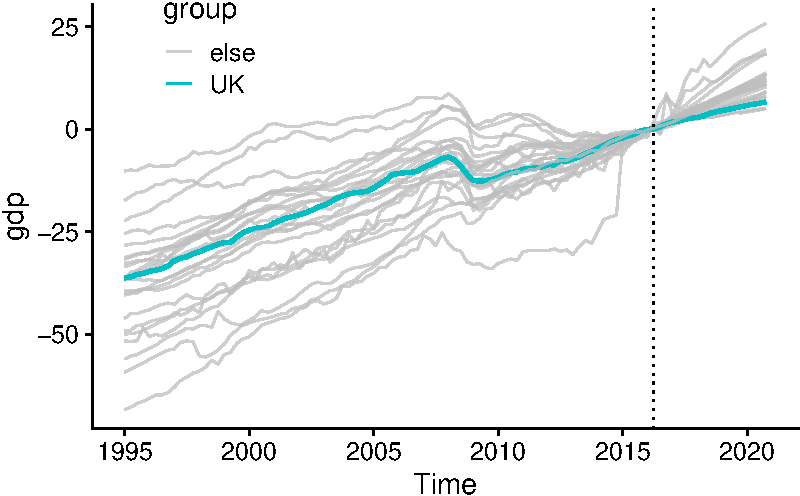
\includegraphics{SyntheticControl_files/figure-pdf/fig-bipv-1.pdf}

}

\caption{\label{fig-bipv}BIP relativ zu 2016}

\end{figure}%

Abbildung~\ref{fig-bipv} zeigt, dass das BIP von Großbritannien zwar
auch nach dem Brexit-Referendum (gepunktete Linie) gewachsen ist, jedoch
vergleichsweise schwach. Eine Analyse mit SCM kann statistische Evidenz
für den mutmaßlich negativen Effekt des Referendums auf das Wachstum in
den Folgeperioden liefern.

Wir laden nun das Paket \texttt{Synth} und bereiten die Daten für die
Analyse vor.

\begin{Shaded}
\begin{Highlighting}[]
\CommentTok{\# R{-}Paket \textquotesingle{}Synth\textquotesingle{} laden}
\FunctionTok{library}\NormalTok{(Synth)}

\CommentTok{\# Daten für die Optimierung vorbereiten}
\NormalTok{dataprep\_out }\OtherTok{\textless{}{-}} \FunctionTok{dataprep}\NormalTok{(}
  \AttributeTok{foo =}\NormalTok{ brexit, }
  \AttributeTok{predictors =} \FunctionTok{c}\NormalTok{(}
    \StringTok{"ConGDP"}\NormalTok{, }\StringTok{"InvGDP"}\NormalTok{, }
    \StringTok{"ExpGDP"}\NormalTok{, }\StringTok{"ImpGDP"}\NormalTok{, }
    \StringTok{"LPG"}\NormalTok{, }\StringTok{"EmpSha"}
\NormalTok{  ), }
  \AttributeTok{dependent =} \StringTok{"gdp"}\NormalTok{, }
  \AttributeTok{unit.variable =} \StringTok{"ID"}\NormalTok{,}
  \AttributeTok{time.variable =} \StringTok{"Time"}\NormalTok{, }
  \AttributeTok{treatment.identifier =} \DecValTok{23}\NormalTok{, }
  \AttributeTok{controls.identifier =}\NormalTok{ (brexit}\SpecialCharTok{$}\NormalTok{ID }\SpecialCharTok{\%\textgreater{}\%} \FunctionTok{unique}\NormalTok{())[}\SpecialCharTok{{-}}\DecValTok{23}\NormalTok{], }
  \AttributeTok{time.predictors.prior =} \FunctionTok{seq}\NormalTok{(}\DecValTok{1995}\NormalTok{, }\FloatTok{2016.25}\NormalTok{, .}\DecValTok{25}\NormalTok{),}
  \AttributeTok{time.optimize.ssr =} \FunctionTok{seq}\NormalTok{(}\DecValTok{1995}\NormalTok{, }\FloatTok{2016.25}\NormalTok{, .}\DecValTok{25}\NormalTok{),}
  \AttributeTok{unit.names.variable =} \StringTok{"Country"}
\NormalTok{)}
\end{Highlighting}
\end{Shaded}

Anhand der vorbereiteten Daten \texttt{dataprep\_out} wird nun die
Bestimmung der Gewichte mit \texttt{Synth::synth()} durchgeführt.

\begin{Shaded}
\begin{Highlighting}[]
\CommentTok{\# Gewichte per Optimierung bestimmen}
\NormalTok{synth\_out }\OtherTok{\textless{}{-}} \FunctionTok{synth}\NormalTok{(dataprep\_out)}
\end{Highlighting}
\end{Shaded}

\begin{verbatim}

X1, X0, Z1, Z0 all come directly from dataprep object.


**************** 
 searching for synthetic control unit  
 

**************** 
**************** 
**************** 

MSPE (LOSS V): 0.6083746 

solution.v:
 0.1488472 0.08840361 0.1480946 0.153318 0.1815462 0.2797904 

solution.w:
 1.42199e-05 4.00616e-05 8.47284e-05 0.00014488 4.45754e-05 4.84009e-05 0.001608051 4.77577e-05 0.06654494 2.07094e-05 0.1446237 1.188e-05 2.377e-06 0.04837474 1.33542e-05 0.0001405933 4.61625e-05 0.0001592545 1.49993e-05 4.14211e-05 3.78112e-05 0.0002273924 0.737708 
\end{verbatim}

\texttt{Synth::synth()} gibt Infos über den Optimierungsprozess und
dessen Ergebnisse automatisch in der Konsole aus. Wir können diese mit
\texttt{Synth::synth.tab()} leicht tabellarisch zusammenfassen und mit
\texttt{gt::gt()} darstellen.

\begin{Shaded}
\begin{Highlighting}[]
\CommentTok{\# Zusammenfassung der Ergebnisse}
\NormalTok{(}
\NormalTok{  tb }\OtherTok{\textless{}{-}} \FunctionTok{synth.tab}\NormalTok{(}
    \AttributeTok{synth.res =}\NormalTok{ synth\_out, }
    \AttributeTok{dataprep.res =}\NormalTok{ dataprep\_out}
\NormalTok{  )  }
\NormalTok{)}
\end{Highlighting}
\end{Shaded}

\begin{verbatim}
$tab.pred
       Treated Synthetic Sample Mean
ConGDP   0.655     0.635       0.534
InvGDP   0.168     0.202       0.226
ExpGDP   0.254     0.219       0.454
ImpGDP   0.256     0.232       0.423
LPG      0.003     0.003       0.003
EmpSha   0.634     0.625       0.611

$tab.v
       v.weights
ConGDP 0.149    
InvGDP 0.088    
ExpGDP 0.148    
ImpGDP 0.153    
LPG    0.182    
EmpSha 0.28     

$tab.w
   w.weights      unit.names unit.numbers
1      0.000       Australia            1
2      0.000         Austria            2
3      0.000         Belgium            3
4      0.000          Canada            4
5      0.000         Finland            5
6      0.000          France            6
7      0.002         Germany            7
8      0.000         Hungary            8
9      0.067         Iceland            9
10     0.000         Ireland           10
11     0.145           Italy           11
12     0.000           Japan           12
13     0.000           Korea           13
14     0.048      Luxembourg           14
15     0.000     Netherlands           15
16     0.000     New Zealand           16
17     0.000          Norway           17
18     0.000        Portugal           18
19     0.000 Slovak Republic           19
20     0.000           Spain           20
21     0.000          Sweden           21
22     0.000     Switzerland           22
24     0.738   United States           24

$tab.loss
       Loss W    Loss V
[1,] 0.135733 0.6083746
\end{verbatim}

Für die tabellarische Darstellung mit \texttt{gt::gt()} berücksichtigen
wir lediglich Volkswirtschaften mit Gewicht \textgreater{} .0001.

\begin{Shaded}
\begin{Highlighting}[]
\CommentTok{\# Darstellung mit gt()}
\NormalTok{tb}\SpecialCharTok{$}\NormalTok{tab.w }\SpecialCharTok{\%\textgreater{}\%} 
  \CommentTok{\# Berücksichtige nur Länder mit relevanten Gewichten}
  \FunctionTok{filter}\NormalTok{(w.weights }\SpecialCharTok{\textgreater{}}\NormalTok{ .}\DecValTok{0001}\NormalTok{) }\SpecialCharTok{\%\textgreater{}\%} 
  \FunctionTok{arrange}\NormalTok{(}\FunctionTok{desc}\NormalTok{(w.weights)) }\SpecialCharTok{\%\textgreater{}\%} 
\NormalTok{  gt}\SpecialCharTok{::}\FunctionTok{gt}\NormalTok{() }\SpecialCharTok{\%\textgreater{}\%}
\NormalTok{  tabopts}
\end{Highlighting}
\end{Shaded}

\begin{longtable}{rlr}

\caption{\label{tbl-brexitcw}Gewichte für den synthetischen
UK-Doppelgänger}

\tabularnewline

\toprule
w.weights & unit.names & unit.numbers \\ 
\midrule\addlinespace[2.5pt]
$0.738$ & United States & $24$ \\ 
$0.145$ & Italy & $11$ \\ 
$0.067$ & Iceland & $9$ \\ 
$0.048$ & Luxembourg & $14$ \\ 
$0.002$ & Germany & $7$ \\ 
\bottomrule

\end{longtable}

Der synthetische UK-Doppelgänger kann nun gemäß der Vorschrift
\eqref{eq:dgkonst} konstruiert werden. Wir erzeugen hierzu ein
\texttt{tibble}-Objekt mit den entsprechenden ID-Variablen.

\begin{Shaded}
\begin{Highlighting}[]
\CommentTok{\# Doppelgänger konstruieren}
\NormalTok{doppelganger }\OtherTok{\textless{}{-}} \FunctionTok{left\_join}\NormalTok{(}
  \AttributeTok{x =}\NormalTok{ brexit, }
  \AttributeTok{y =}\NormalTok{ tb}\SpecialCharTok{$}\NormalTok{tab.w, }
  \AttributeTok{by =} \FunctionTok{c}\NormalTok{(}\StringTok{"Country"} \OtherTok{=} \StringTok{"unit.names"}\NormalTok{)}
\NormalTok{) }\SpecialCharTok{\%\textgreater{}\%} 
  \FunctionTok{select}\NormalTok{(Time, Year, Country, gdp, w.weights) }\SpecialCharTok{\%\textgreater{}\%}
  \FunctionTok{group\_by}\NormalTok{(Time, Year) }\SpecialCharTok{\%\textgreater{}\%}
  \FunctionTok{summarise}\NormalTok{(}
    \AttributeTok{gdp =} \FunctionTok{sum}\NormalTok{(gdp }\SpecialCharTok{*}\NormalTok{ w.weights, }\AttributeTok{na.rm =}\NormalTok{ T)}
\NormalTok{  ) }\SpecialCharTok{\%\textgreater{}\%}
  \FunctionTok{mutate}\NormalTok{(}\AttributeTok{type =} \StringTok{"Doppelgaenger"}\NormalTok{) }\SpecialCharTok{\%\textgreater{}\%}
  \FunctionTok{ungroup}\NormalTok{()}

\FunctionTok{glimpse}\NormalTok{(doppelganger)}
\end{Highlighting}
\end{Shaded}

\begin{verbatim}
Rows: 104
Columns: 4
$ Time <dbl> 1995.00, 1995.25, 1995.50, 1995.75, 1996.00, 1996.25, 1996.50, 19~
$ Year <dbl> 1995, 1995, 1995, 1995, 1996, 1996, 1996, 1996, 1997, 1997, 1997,~
$ gdp  <dbl> -36.87991, -36.70512, -36.32948, -35.72637, -35.34392, -34.57688,~
$ type <chr> "Doppelgaenger", "Doppelgaenger", "Doppelgaenger", "Doppelgaenger~
\end{verbatim}

Für die nachfolgenden Schritte der Analyse führen wir das beobachtete
GDP für Großbritannien mit dem syntethischen GDP des Doppelgängers
zusammen.

\begin{Shaded}
\begin{Highlighting}[]
\CommentTok{\# tibble mit UK{-}GDP erstellen}
\NormalTok{UK }\OtherTok{\textless{}{-}}\NormalTok{ brexit }\SpecialCharTok{\%\textgreater{}\%} 
  \FunctionTok{filter}\NormalTok{(Country }\SpecialCharTok{==} \StringTok{"United Kingdom"}\NormalTok{) }\SpecialCharTok{\%\textgreater{}\%} 
  \FunctionTok{select}\NormalTok{(Time, Year, gdp) }\SpecialCharTok{\%\textgreater{}\%}
  \FunctionTok{mutate}\NormalTok{(}\AttributeTok{type =} \StringTok{"UK"}\NormalTok{)}

\CommentTok{\# UK und Doppelgänger zusammenführen}
\NormalTok{the\_gdps }\OtherTok{\textless{}{-}} \FunctionTok{bind\_rows}\NormalTok{(}
\NormalTok{  doppelganger, UK}
\NormalTok{)}
\end{Highlighting}
\end{Shaded}

Für einen Vergleich von UK- und Doppelgänger-BIP folgen wir Born u.~a.
(2019) und berechnen die Differenz der BIP über den gesamten Zeitraum,
die so genannte \emph{Doppelgänger-Gap}.

\begin{Shaded}
\begin{Highlighting}[]
\CommentTok{\# UK{-}Doppelgänger{-}Gap berechnen}
\NormalTok{gdp\_gap }\OtherTok{\textless{}{-}}\NormalTok{ the\_gdps }\SpecialCharTok{\%\textgreater{}\%} 
  \FunctionTok{pivot\_wider}\NormalTok{(}
    \AttributeTok{values\_from =}\NormalTok{ gdp, }
    \AttributeTok{names\_from =} \StringTok{"type"}
\NormalTok{  ) }\SpecialCharTok{\%\textgreater{}\%}
  \FunctionTok{mutate}\NormalTok{(}\AttributeTok{gdp\_gap =}\NormalTok{ UK }\SpecialCharTok{{-}}\NormalTok{ Doppelgaenger)}
\end{Highlighting}
\end{Shaded}

Als ein Maß für die Unsicherheit bei der Schätzung des GDPs für den
Doppelgänger berechnen Born u.~a. (2019) die Standardabweichung der
Doppelgänger-Gap für den Zeitraum \emph{vor} dem Brexit-Referendum.

\begin{Shaded}
\begin{Highlighting}[]
\CommentTok{\# Standardabweichung der Gap vor dem Brexit{-}Vote}
\NormalTok{sd\_gap }\OtherTok{\textless{}{-}}\NormalTok{ gdp\_gap }\SpecialCharTok{\%\textgreater{}\%}
  \FunctionTok{filter}\NormalTok{(Time }\SpecialCharTok{\textless{}} \FloatTok{2016.25}\NormalTok{) }\SpecialCharTok{\%\textgreater{}\%} 
  \FunctionTok{summarise}\NormalTok{(}
    \AttributeTok{sd =} \FunctionTok{sd}\NormalTok{(gdp\_gap)}
\NormalTok{  ) }\SpecialCharTok{\%\textgreater{}\%} 
  \FunctionTok{pull}\NormalTok{(sd)}
\end{Highlighting}
\end{Shaded}

Wir nutzen nun \texttt{ggplot2::ggplot()}, um den syntetischen
Doppelgänger und das BIP für Großbritannien über den gesamten Zeitraum
darzustellen. Für die Darstellung von Unsicherheit bei der Konstruktion
des Doppelgängers unterlegen wir die Doppelgänger-Zeitreihe mit einer
Schattierung in der Breite der geschätzten Standardabweichung von 0.78
für die Periode vor dem Referendum.

\begin{Shaded}
\begin{Highlighting}[]
\NormalTok{(}
\NormalTok{  p\_gdp }\OtherTok{\textless{}{-}} \FunctionTok{ggplot}\NormalTok{() }\SpecialCharTok{+}
    \CommentTok{\# 1{-}SD{-}Band um das Doppelgänger{-}GDP}
    \FunctionTok{geom\_ribbon}\NormalTok{(}
      \AttributeTok{data =}\NormalTok{ the\_gdps }\SpecialCharTok{\%\textgreater{}\%} 
        \FunctionTok{filter}\NormalTok{(type }\SpecialCharTok{==} \StringTok{"Doppelgaenger"}\NormalTok{), }
      \AttributeTok{mapping =} \FunctionTok{aes}\NormalTok{(}
        \AttributeTok{x =}\NormalTok{ Time, }
        \AttributeTok{ymin =}\NormalTok{ gdp }\SpecialCharTok{{-}}\NormalTok{ sd\_gap, }
        \AttributeTok{ymax =}\NormalTok{ gdp }\SpecialCharTok{+}\NormalTok{ sd\_gap}
\NormalTok{      ), }
      \AttributeTok{fill =} \FunctionTok{alpha}\NormalTok{(}\StringTok{"red"}\NormalTok{, }\AttributeTok{alpha =}\NormalTok{ .}\DecValTok{2}\NormalTok{), }
      \AttributeTok{color =} \StringTok{"white"}
\NormalTok{    ) }\SpecialCharTok{+}
    \CommentTok{\# UK{-} und Doppelgänger{-}GDP}
    \FunctionTok{geom\_line}\NormalTok{(}
      \AttributeTok{data =}\NormalTok{ the\_gdps, }
      \AttributeTok{mapping =} \FunctionTok{aes}\NormalTok{(}
        \AttributeTok{x =}\NormalTok{ Time, }
        \AttributeTok{y =}\NormalTok{ gdp, }
        \AttributeTok{col =}\NormalTok{ type}
\NormalTok{      ),}
      \AttributeTok{lwd =} \DecValTok{1}
\NormalTok{    ) }\SpecialCharTok{+}
    \CommentTok{\# Brexit{-}Referendum}
    \FunctionTok{geom\_vline}\NormalTok{(}
      \AttributeTok{xintercept =} \FloatTok{2016.25}\NormalTok{, }
      \AttributeTok{lty =} \StringTok{"dotted"}
\NormalTok{    ) }\SpecialCharTok{+}
    \FunctionTok{scale\_color\_discrete}\NormalTok{(}\AttributeTok{name =} \StringTok{""}\NormalTok{) }\SpecialCharTok{+}
    \CommentTok{\# Legende hinzufügen}
\NormalTok{    cowplot}\SpecialCharTok{::}\FunctionTok{theme\_cowplot}\NormalTok{() }\SpecialCharTok{+}
    \FunctionTok{theme}\NormalTok{(}\AttributeTok{legend.position =} \FunctionTok{c}\NormalTok{(.}\DecValTok{025}\NormalTok{, .}\DecValTok{9}\NormalTok{))  }
\NormalTok{)}
\end{Highlighting}
\end{Shaded}

\begin{figure}[t]

\centering{

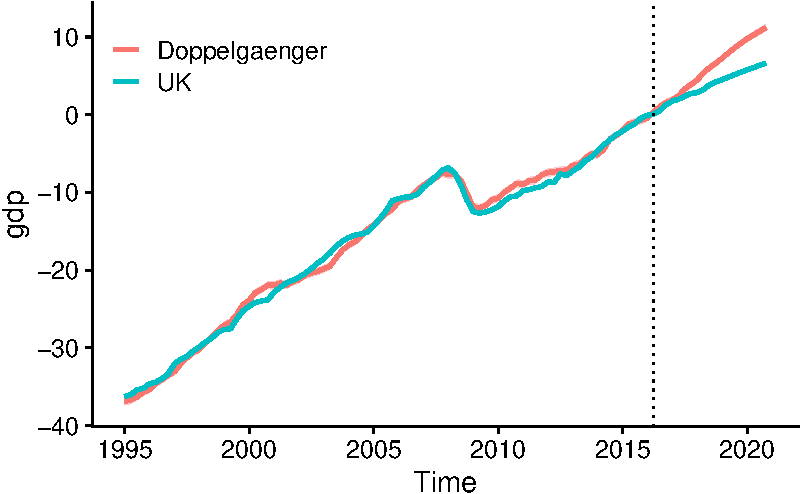
\includegraphics{SyntheticControl_files/figure-pdf/fig-ukuksdg-1.pdf}

}

\caption{\label{fig-ukuksdg}UK-BIP und synthetischer Doppelgänger}

\end{figure}%

Abbildung~\ref{fig-ukuksdg} zeigt, dass der synthetische Doppelgänger
über weite Teile der Vorperiode eine gute Anpassung an das beobachtete
BIP von Großbritannien aufweist, insbesondere für den Zeitraum
unmittelbar vor dem Brexit-Referendum. Nach dem Referendum zeigt sich
bereits nach wenigen Quartalen eine deutliche Abweichung zwischen der
geschätzten und der beobachteten Trajektorie. Eine Beschränkung der in
\texttt{p\_gdp} verwendeten Datenpunkte auf einen Bereich nahe des
Referendums bestärkt diese Schlussfolgerung.

\begin{Shaded}
\begin{Highlighting}[]
\CommentTok{\# Close{-}up im Bereich des Referendums}
\NormalTok{p\_gdp }\SpecialCharTok{+}
  \FunctionTok{scale\_x\_continuous}\NormalTok{(}
    \AttributeTok{limits =} \FunctionTok{c}\NormalTok{(}\DecValTok{2015}\NormalTok{, }\DecValTok{2021}\NormalTok{), }
    \AttributeTok{expand =} \FunctionTok{c}\NormalTok{(}\DecValTok{0}\NormalTok{, .}\DecValTok{1}\NormalTok{)}
\NormalTok{    ) }\SpecialCharTok{+}
  \FunctionTok{scale\_y\_continuous}\NormalTok{(}\AttributeTok{limits =} \FunctionTok{c}\NormalTok{(}\SpecialCharTok{{-}}\DecValTok{4}\NormalTok{, }\DecValTok{12}\NormalTok{))}
\end{Highlighting}
\end{Shaded}

\begin{figure}[t]

\centering{

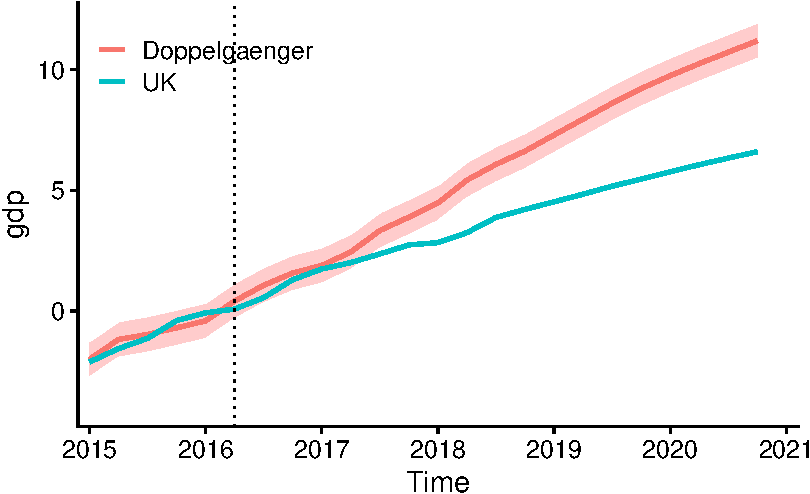
\includegraphics{SyntheticControl_files/figure-pdf/fig-ukuksdgclose-1.pdf}

}

\caption{\label{fig-ukuksdgclose}UK-BIP und synthetischer Doppelgänger
-- Close-Up}

\end{figure}%

In Abbildung~\ref{fig-ukuksdg} ist eine ab Mitte 2017 außerhalb des
Standardabweichungsbereichs verlaufende Divergenz der Zeitreihen zu
erkennen. Diese stellen wir nachfolgend anhand der Doppelgänger-Gap mit
\texttt{ggplot2::ggplot()} dar.

\begin{Shaded}
\begin{Highlighting}[]
\CommentTok{\# BIP{-}Doppelgänger{-}Gap}
\FunctionTok{ggplot}\NormalTok{(}\AttributeTok{data =}\NormalTok{ gdp\_gap) }\SpecialCharTok{+}
  \FunctionTok{geom\_hline}\NormalTok{(}\AttributeTok{yintercept =} \DecValTok{0}\NormalTok{) }\SpecialCharTok{+}
  \FunctionTok{geom\_line}\NormalTok{(}
    \AttributeTok{mapping =} \FunctionTok{aes}\NormalTok{(}\AttributeTok{x =}\NormalTok{ Time, }\AttributeTok{y =}\NormalTok{ gdp\_gap),}
    \AttributeTok{lwd =} \DecValTok{1}
\NormalTok{  ) }\SpecialCharTok{+} 
  \FunctionTok{geom\_ribbon}\NormalTok{(}
    \AttributeTok{mapping =} \FunctionTok{aes}\NormalTok{(}
      \AttributeTok{x =}\NormalTok{ Time, }
      \AttributeTok{ymin =}\NormalTok{ gdp\_gap }\SpecialCharTok{{-}}\NormalTok{ sd\_gap, }
      \AttributeTok{ymax =}\NormalTok{ gdp\_gap }\SpecialCharTok{+}\NormalTok{ sd\_gap}
\NormalTok{    ), }
    \AttributeTok{fill =} \FunctionTok{alpha}\NormalTok{(}\StringTok{"darkgray"}\NormalTok{, }\AttributeTok{alpha =}\NormalTok{ .}\DecValTok{2}\NormalTok{), }
    \AttributeTok{color =} \StringTok{"white"}
\NormalTok{  ) }\SpecialCharTok{+}
  \CommentTok{\# Referendum}
  \FunctionTok{geom\_vline}\NormalTok{(}
    \AttributeTok{xintercept =} \FloatTok{2016.25}\NormalTok{,}
    \AttributeTok{lty =} \StringTok{"dotted"}
\NormalTok{  ) }\SpecialCharTok{+}
  \FunctionTok{scale\_x\_continuous}\NormalTok{(}
    \AttributeTok{expand =} \FunctionTok{c}\NormalTok{(}\DecValTok{0}\NormalTok{, .}\DecValTok{1}\NormalTok{), }
    \AttributeTok{limits =} \FunctionTok{c}\NormalTok{(}\DecValTok{2015}\NormalTok{, }\DecValTok{2021}\NormalTok{)}
\NormalTok{  ) }\SpecialCharTok{+}
  \FunctionTok{scale\_y\_continuous}\NormalTok{(}\AttributeTok{limits =} \FunctionTok{c}\NormalTok{(}\SpecialCharTok{{-}}\DecValTok{6}\NormalTok{, }\FloatTok{1.5}\NormalTok{)) }\SpecialCharTok{+}
\NormalTok{  cowplot}\SpecialCharTok{::}\FunctionTok{theme\_cowplot}\NormalTok{()}
\end{Highlighting}
\end{Shaded}

\begin{figure}[t]

\centering{

\includegraphics{SyntheticControl_files/figure-pdf/fig-ukdggap-1.pdf}

}

\caption{\label{fig-ukdggap}UK-BIP und synthetischer Doppelgänger --
Doppelgänger-Gap}

\end{figure}%

Die in Abbildung~\ref{fig-ukdggap} gezeigte Doppelgänger-Gap stimmt gut
mit dem von Born u.~a. (2019) geschätzten verlorenen Wachstums des BIP
relativ zu 2016 um bis zu 2.5\% bis Ende des Jahres 2018 überein.

Als weiteres Maß für den Effekt des Referendums im Folgezeitraum können
wir die mittlere Doppelgänger-Gap für sämtliche Beobachtungsperioden
nach dem Brexit-Referendum schnell bestimmen.

\begin{Shaded}
\begin{Highlighting}[]
\CommentTok{\# Mittlerer Unterschied nach dem Brexit{-}Referendum}
\NormalTok{gdp\_gap }\SpecialCharTok{\%\textgreater{}\%} 
  \FunctionTok{filter}\NormalTok{(Time }\SpecialCharTok{\textgreater{}} \FloatTok{2016.25}\NormalTok{) }\SpecialCharTok{\%\textgreater{}\%} 
  \FunctionTok{pull}\NormalTok{(gdp\_gap) }\SpecialCharTok{\%\textgreater{}\%} 
  \FunctionTok{mean}\NormalTok{()}
\end{Highlighting}
\end{Shaded}

\begin{verbatim}
[1] -2.343273
\end{verbatim}

\subsection{Placebo-Tests: Grafische
Inferenz}\label{placebo-tests-grafische-inferenz}

Auch für SCM sind Placebo-Tests ein hilfreiches Instrument zur
Überprüfung der Gültigkeit von Studienergebnissen. Eine gründliche
Placebo-Analyse kann festzustellen, ob der beobachtete Effekt
tatsächlich auf die Intervention zurückzuführen ist und nicht auf
unberücksichtigte (möglicherweise unbeobachtbare) Faktoren.

Ein Ansatz ist hierfür ist es, den synthetische-Doppelgänger für
\emph{fiktive Interventionszeitpunkte} vor dem tatsächlichen
Behandlungszeitpunkt zu konstruieren, und die entsprechenden
Trajektorien mit dem ursprünglichen Doppelgänger zu vergleichen. So kann
die Validität der ursprünglichen Doppelgänger-Trajektorie im Hinblick
auf mögliche anderweitige Ereignisse vor der Intervention geprüft
werden: Doppelgänger-Trajektorien für fiktive, frühere Interventionen
sollten sich nicht systematisch von der andhand von Daten bis zur
tatsächlichen Intervention berechneten Trajektorie unterscheiden.

Wir definieren hierzu eine Funktion \texttt{placebo()}, die einen
syntethischen Doppelgänger des BIP Großbritanniens mit Gewichten auf
Basis eines vorgegebenen Interventionszeitpunktes (\texttt{treat})
zurückgibt. Abgesehen vom früheren Interventionszeitpunkt (und der damit
einhergehenden verkleinerten Stichprobe) erfolgt die Berechnung der
Gewichte mit derselben Spezifikation wie zuvor.

\begin{Shaded}
\begin{Highlighting}[]
\CommentTok{\# Funktion für Placebo{-}Doppelgänger:}
\CommentTok{\# Fiktive frühere Intervention}
\NormalTok{placebo }\OtherTok{\textless{}{-}} \ControlFlowTok{function}\NormalTok{(treat) \{}
  
  \CommentTok{\# Datenvorbereitung für fiktives Datum \textquotesingle{}treat\textquotesingle{}}
\NormalTok{  dataprep\_out }\OtherTok{\textless{}{-}} \FunctionTok{dataprep}\NormalTok{(}
    \AttributeTok{foo =}\NormalTok{ brexit, }
    \AttributeTok{predictors =} \FunctionTok{c}\NormalTok{(}
      \StringTok{"ConGDP"}\NormalTok{, }\StringTok{"InvGDP"}\NormalTok{,}
      \StringTok{"ExpGDP"}\NormalTok{, }\StringTok{"ImpGDP"}\NormalTok{,}
      \StringTok{"LPG"}\NormalTok{, }\StringTok{"EmpSha"}
\NormalTok{    ), }
    \AttributeTok{dependent =} \StringTok{"gdp"}\NormalTok{, }
    \AttributeTok{unit.variable =} \StringTok{"ID"}\NormalTok{,}
    \AttributeTok{time.variable =} \StringTok{"Time"}\NormalTok{, }
    \AttributeTok{treatment.identifier =} \DecValTok{23}\NormalTok{, }
    \AttributeTok{controls.identifier =}\NormalTok{ (brexit}\SpecialCharTok{$}\NormalTok{ID }\SpecialCharTok{\%\textgreater{}\%} \FunctionTok{unique}\NormalTok{())[}\SpecialCharTok{{-}}\DecValTok{23}\NormalTok{], }
    \AttributeTok{time.predictors.prior =} \FunctionTok{seq}\NormalTok{(}\DecValTok{1995}\NormalTok{, treat, .}\DecValTok{25}\NormalTok{),}
    \AttributeTok{time.optimize.ssr =} \FunctionTok{seq}\NormalTok{(}\DecValTok{1995}\NormalTok{, treat, .}\DecValTok{25}\NormalTok{),}
    \AttributeTok{unit.names.variable =} \StringTok{"Country"}
\NormalTok{    )}
  
  \CommentTok{\# Doppelgänger bestimmen}
\NormalTok{  synth\_out }\OtherTok{\textless{}{-}} \FunctionTok{quietly}\NormalTok{(synth)(dataprep\_out)}\SpecialCharTok{$}\NormalTok{result}
  
  \CommentTok{\# Ergebnisse auslesen}
\NormalTok{  tb }\OtherTok{\textless{}{-}} \FunctionTok{synth.tab}\NormalTok{(}
    \AttributeTok{synth.res =}\NormalTok{ synth\_out, }
    \AttributeTok{dataprep.res =}\NormalTok{ dataprep\_out}
\NormalTok{    )}
  
  \FunctionTok{return}\NormalTok{(}
    
    \CommentTok{\# Doppelgänger konstruieren }
    \FunctionTok{left\_join}\NormalTok{(}
      \AttributeTok{x =}\NormalTok{ brexit, }
      \AttributeTok{y =}\NormalTok{ tb}\SpecialCharTok{$}\NormalTok{tab.w, }
      \AttributeTok{by =} \FunctionTok{c}\NormalTok{(}\StringTok{"Country"} \OtherTok{=} \StringTok{"unit.names"}\NormalTok{)}
\NormalTok{    ) }\SpecialCharTok{\%\textgreater{}\%} 
      \FunctionTok{select}\NormalTok{(Time, Country, gdp, w.weights) }\SpecialCharTok{\%\textgreater{}\%}
      \FunctionTok{group\_by}\NormalTok{(Time) }\SpecialCharTok{\%\textgreater{}\%}
      \FunctionTok{summarise}\NormalTok{(}
        \AttributeTok{gdp =} \FunctionTok{sum}\NormalTok{(gdp }\SpecialCharTok{*}\NormalTok{ w.weights, }\AttributeTok{na.rm =}\NormalTok{ T)}
\NormalTok{      ) }\SpecialCharTok{\%\textgreater{}\%}
      \FunctionTok{mutate}\NormalTok{(}\AttributeTok{type =} \FunctionTok{paste0}\NormalTok{(}\StringTok{"Placebo"}\NormalTok{, treat))  }
\NormalTok{    )}
  
\NormalTok{\}}
\end{Highlighting}
\end{Shaded}

Wie in Born u.~a. (2019) berechnen wir nun 12 Placebo-Doppelgänger des
BIP von Großbritannien für fiktive Zeitpunkte eines Referendums über
sämtliche Quartale im Zeitraum 2010-Q1 bis 2016-Q1. Dies ist komfortabel
durch Iteration von \texttt{placebo()} über diese Zeitpunkte mit
\texttt{purrr::map\_dfr()} umsetzbar.

\begin{Shaded}
\begin{Highlighting}[]
\CommentTok{\# Iteration über fiktive frühere Referenden}
\NormalTok{placebos\_tbl }\OtherTok{\textless{}{-}} \FunctionTok{map\_dfr}\NormalTok{(}
  \AttributeTok{.x =} \FunctionTok{seq}\NormalTok{(}\DecValTok{2010}\NormalTok{, }\DecValTok{2016}\NormalTok{, .}\DecValTok{25}\NormalTok{), }
  \AttributeTok{.f =}\NormalTok{  \textbackslash{}(x) }\FunctionTok{placebo}\NormalTok{(x) }
\NormalTok{)}
\end{Highlighting}
\end{Shaded}

\texttt{placebos\_tbl} ist ein \texttt{tibble}-Objekt im tidy-Format.
Wir können die Placebo-Doppelgänger sowie den ursprünglich berechneten
Doppelgänger und das tatsächliche BIP also ähnlich wie in
Abbildung~\ref{fig-ukuksdg} mit \texttt{ggplot2::ggplot()} darstellen.

\begin{Shaded}
\begin{Highlighting}[]
\CommentTok{\# Vergleich mit Placebo{-}Doppelgänger}
\NormalTok{(}
\NormalTok{  p\_UKDG }\OtherTok{\textless{}{-}} \FunctionTok{ggplot}\NormalTok{(}
    \AttributeTok{data =}\NormalTok{ placebos\_tbl,}
    \AttributeTok{mapping =} \FunctionTok{aes}\NormalTok{(}
      \AttributeTok{x =}\NormalTok{ Time, }
      \AttributeTok{y =}\NormalTok{ gdp, }
      \AttributeTok{group =}\NormalTok{ type}
\NormalTok{    )}
\NormalTok{  ) }\SpecialCharTok{+}
    \CommentTok{\# Placebos (mit jitter)}
    \FunctionTok{geom\_line}\NormalTok{(}
      \AttributeTok{lwd =}\NormalTok{ .}\DecValTok{25}\NormalTok{, }
      \AttributeTok{col =} \StringTok{"gray80"}\NormalTok{,}
      \AttributeTok{position =} \FunctionTok{position\_jitter}\NormalTok{(}\AttributeTok{height =}\NormalTok{ .}\DecValTok{25}\NormalTok{)}
\NormalTok{    ) }\SpecialCharTok{+}
    \CommentTok{\# Ursprünglicher Doppelgänger}
    \FunctionTok{geom\_line}\NormalTok{(}
      \AttributeTok{data =}\NormalTok{ the\_gdps }\SpecialCharTok{\%\textgreater{}\%} 
        \FunctionTok{filter}\NormalTok{(type }\SpecialCharTok{==} \StringTok{"Doppelgaenger"}\NormalTok{), }
      \AttributeTok{mapping =} \FunctionTok{aes}\NormalTok{(}\AttributeTok{col =}\NormalTok{ type), }
      \AttributeTok{lwd =} \DecValTok{1}
\NormalTok{    ) }\SpecialCharTok{+}
    \CommentTok{\# Beobachtetes BIP}
    \FunctionTok{geom\_line}\NormalTok{(}
      \AttributeTok{data =}\NormalTok{ the\_gdps }\SpecialCharTok{\%\textgreater{}\%} 
        \FunctionTok{filter}\NormalTok{(type }\SpecialCharTok{==} \StringTok{"UK"}\NormalTok{), }
      \AttributeTok{mapping =} \FunctionTok{aes}\NormalTok{(}\AttributeTok{col =}\NormalTok{ type), }
      \AttributeTok{lwd =} \DecValTok{1}
\NormalTok{    ) }\SpecialCharTok{+}
    \CommentTok{\# Intikator für Referendum}
    \FunctionTok{geom\_vline}\NormalTok{(}\AttributeTok{xintercept =} \FloatTok{2016.25}\NormalTok{, }\AttributeTok{lty =} \StringTok{"dotted"}\NormalTok{) }\SpecialCharTok{+}
    \CommentTok{\# Formatierung}
\NormalTok{    cowplot}\SpecialCharTok{::}\FunctionTok{theme\_cowplot}\NormalTok{() }\SpecialCharTok{+}
    \FunctionTok{theme}\NormalTok{(}\AttributeTok{legend.position =} \FunctionTok{c}\NormalTok{(.}\DecValTok{05}\NormalTok{, .}\DecValTok{9}\NormalTok{))}
\NormalTok{)}
\end{Highlighting}
\end{Shaded}

\begin{figure}[t]

\centering{

\includegraphics{SyntheticControl_files/figure-pdf/fig-pdgukbip-1.pdf}

}

\caption{\label{fig-pdgukbip}Placebo-Doppelgänger}

\end{figure}%

\begin{Shaded}
\begin{Highlighting}[]
\CommentTok{\# Close{-}up bei Referendum}
\NormalTok{p\_UKDG }\SpecialCharTok{+}
      \FunctionTok{scale\_x\_continuous}\NormalTok{(}
      \AttributeTok{limits =} \FunctionTok{c}\NormalTok{(}\DecValTok{2015}\NormalTok{, }\DecValTok{2021}\NormalTok{), }\AttributeTok{expand =} \FunctionTok{c}\NormalTok{(}\DecValTok{0}\NormalTok{, .}\DecValTok{05}\NormalTok{)}
\NormalTok{    ) }\SpecialCharTok{+}
      \FunctionTok{scale\_y\_continuous}\NormalTok{(}
      \AttributeTok{limits =} \FunctionTok{c}\NormalTok{(}\SpecialCharTok{{-}}\DecValTok{3}\NormalTok{, }\DecValTok{13}\NormalTok{),  }\AttributeTok{expand =} \FunctionTok{c}\NormalTok{(}\DecValTok{0}\NormalTok{, }\DecValTok{0}\NormalTok{)}
\NormalTok{    )}
\end{Highlighting}
\end{Shaded}

\begin{figure}[t]

\centering{

\includegraphics{SyntheticControl_files/figure-pdf/fig-pdgukbipcu-1.pdf}

}

\caption{\label{fig-pdgukbipcu}Placebo-Doppelgänger -- Close-Up}

\end{figure}%

Beachte, dass \texttt{position\ =\ position\_jitter(height\ =\ .25)}
eine zufällige, kleine Verschiebung (jitter) der Trajektorien der
Placebo-Doppelgänger für eine bessere Unterscheidbarkeit bewirkt.
Abbildung~\ref{fig-pdgukbip} und Abbildung~\ref{fig-pdgukbipcu} zeigen,
dass sich die Placebo-Pfade für fiktive frühere Referenden (grau) nicht
systematisch vom ursprünglich berechneten synthetischen Doppelgänger
(rot) unterscheiden. Insbesondere finden wir keinen Rückgang der
synthetischen BIP relativ zum beobachteten BIP für Großbritannien
\emph{vor} dem Referendum. Deutliche Abweichungen vom tatsächlichen BIP
ergeben sich erst jenseits der tatsächlichen Referendums. Diese
Placebo-Analyse bekräftigt also die Validität der Konstruktion des
``Benchmark-Doppelgängers'' für die Periode bis 2016-Q2 und die
Schätzung des kausalen Effekts des Referendums anhand der entsprechenden
Doppelgänger-Gap.

Ein weiterer Placebo-Test in Born u.~a. (2019) ist ein Vergleich der
Doppelgänger-Gap Großbritanniens mit Doppelgänger-Gaps für fiktive
Referenden in 2016-Q2 in Ländern mit wesentlichem Einfluss bei der
Konstruktion des synthetischen Doppelgängers für Großbritannien: Die
Schätzung des kausalen Effekts des Referendums auf das BIP in
Großbritannien ist glaubwürdig, wenn lediglich die Doppelgänger-Gap für
Großbritannien durch das Referendum beeinflusst wird, \emph{nicht} aber
die Doppelgänger-Gaps für Länder in der Kontrollgruppe.

Für diese grafische Placebo-Analyse modifizieren wir die Funktion
\texttt{placebo()} entsprechend. \texttt{placebo\_gap()} berechnet die
Doppelgänger-Gap für das mit \texttt{treat} identifizierte Land. Das
\texttt{if}-Statement zu Beginn stellt sicher, dass Großbritannien
\emph{nicht} als Kontroll-Einheit für die Placebo-Gaps verwendet wird.

\begin{Shaded}
\begin{Highlighting}[]
\CommentTok{\# Funktion für Placebo{-}Gaps}
\NormalTok{placebo\_gap }\OtherTok{\textless{}{-}} \ControlFlowTok{function}\NormalTok{(treat) \{}
  
  \CommentTok{\# Kontrollgruppe definieren}
  \ControlFlowTok{if}\NormalTok{(treat }\SpecialCharTok{!=} \DecValTok{23}\NormalTok{) \{}
\NormalTok{    controls }\OtherTok{\textless{}{-}}\NormalTok{ (}\DecValTok{1}\SpecialCharTok{:}\DecValTok{24}\NormalTok{)[}\SpecialCharTok{{-}}\FunctionTok{c}\NormalTok{(}\DecValTok{23}\NormalTok{, treat)]}
\NormalTok{  \} }\ControlFlowTok{else}\NormalTok{ \{}
\NormalTok{    controls }\OtherTok{\textless{}{-}}\NormalTok{ (}\DecValTok{1}\SpecialCharTok{:}\DecValTok{24}\NormalTok{)[}\SpecialCharTok{{-}}\DecValTok{23}\NormalTok{]}
\NormalTok{  \}}
  
  \CommentTok{\# Daten vorbereiten}
\NormalTok{  dataprep\_out }\OtherTok{\textless{}{-}} \FunctionTok{dataprep}\NormalTok{(}
    \AttributeTok{foo =}\NormalTok{ brexit, }
    \AttributeTok{predictors =} \FunctionTok{c}\NormalTok{(}
      \StringTok{"ConGDP"}\NormalTok{, }\StringTok{"InvGDP"}\NormalTok{,}
      \StringTok{"ExpGDP"}\NormalTok{, }\StringTok{"ImpGDP"}\NormalTok{,}
      \StringTok{"LPG"}\NormalTok{, }\StringTok{"EmpSha"}
\NormalTok{    ), }
    \AttributeTok{dependent =} \StringTok{"gdp"}\NormalTok{, }
    \AttributeTok{unit.variable =} \StringTok{"ID"}\NormalTok{,}
    \AttributeTok{time.variable =} \StringTok{"Time"}\NormalTok{, }
    \AttributeTok{treatment.identifier =}\NormalTok{ treat, }
    \AttributeTok{controls.identifier =}\NormalTok{ controls, }
    \AttributeTok{time.predictors.prior =} \FunctionTok{seq}\NormalTok{(}\DecValTok{1995}\NormalTok{, }\FloatTok{2016.25}\NormalTok{, .}\DecValTok{25}\NormalTok{),}
    \AttributeTok{time.optimize.ssr =} \FunctionTok{seq}\NormalTok{(}\DecValTok{1995}\NormalTok{, }\FloatTok{2016.25}\NormalTok{, .}\DecValTok{25}\NormalTok{),}
    \AttributeTok{unit.names.variable =} \StringTok{"Country"}
\NormalTok{  )}
  
  \CommentTok{\# Gewichte bestimmen}
\NormalTok{  synth\_out }\OtherTok{\textless{}{-}} \FunctionTok{quietly}\NormalTok{(synth)(dataprep\_out)}\SpecialCharTok{$}\NormalTok{result}
  
  \CommentTok{\# Ergebnisse zusammenfassen}
\NormalTok{  tb }\OtherTok{\textless{}{-}} \FunctionTok{synth.tab}\NormalTok{(}
    \AttributeTok{synth.res =}\NormalTok{ synth\_out, }
    \AttributeTok{dataprep.res =}\NormalTok{ dataprep\_out}
\NormalTok{  )}
  
  \CommentTok{\# Doppelgänger bestimmen}
\NormalTok{  doppel }\OtherTok{\textless{}{-}} \FunctionTok{left\_join}\NormalTok{(}
    \AttributeTok{x =}\NormalTok{ brexit, }
    \AttributeTok{y =}\NormalTok{ tb}\SpecialCharTok{$}\NormalTok{tab.w, }
    \AttributeTok{by =} \FunctionTok{c}\NormalTok{(}\StringTok{"Country"} \OtherTok{=} \StringTok{"unit.names"}\NormalTok{)}
\NormalTok{  ) }\SpecialCharTok{\%\textgreater{}\%} 
    \FunctionTok{select}\NormalTok{(Time, gdp, Country, w.weights) }\SpecialCharTok{\%\textgreater{}\%}
    \FunctionTok{group\_by}\NormalTok{(Time) }\SpecialCharTok{\%\textgreater{}\%}
    \FunctionTok{summarise}\NormalTok{(}
      \AttributeTok{gdp\_synth =} \FunctionTok{sum}\NormalTok{(gdp }\SpecialCharTok{*}\NormalTok{ w.weights, }\AttributeTok{na.rm =}\NormalTok{ T), }
\NormalTok{    )}
  
  \CommentTok{\# Beobachtetes BIP auslesen}
\NormalTok{  gdp }\OtherTok{\textless{}{-}}\NormalTok{ brexit }\SpecialCharTok{\%\textgreater{}\%} \FunctionTok{filter}\NormalTok{(ID }\SpecialCharTok{==}\NormalTok{ treat) }\SpecialCharTok{\%\textgreater{}\%} \FunctionTok{pull}\NormalTok{(gdp)}
  
  \FunctionTok{return}\NormalTok{(}
    
    \CommentTok{\# Doppelgänger{-}Gap berechnen}
\NormalTok{    doppel }\SpecialCharTok{\%\textgreater{}\%} 
      \FunctionTok{mutate}\NormalTok{(}
        \AttributeTok{ID =}\NormalTok{ treat,}
        \AttributeTok{gdp =}\NormalTok{ gdp,}
        \AttributeTok{gdp\_gap =}\NormalTok{ gdp }\SpecialCharTok{{-}}\NormalTok{ gdp\_synth}
\NormalTok{      )}
    
\NormalTok{  )}
  
\NormalTok{\}}
\end{Highlighting}
\end{Shaded}

Für die Berechnung der Placebo-Gaps iterieren wir über die Indizes der
in Tabelle~\ref{tbl-brexitcw} gelisteten Volkswirtschaften der
Kontrollgruppe für Großbritannien.

\begin{Shaded}
\begin{Highlighting}[]
\CommentTok{\# Indizes für "Donor Countries" und UK}
\NormalTok{donors\_and\_UK }\OtherTok{\textless{}{-}}\NormalTok{ brexit }\SpecialCharTok{\%\textgreater{}\%} 
  \FunctionTok{select}\NormalTok{(ID, Country) }\SpecialCharTok{\%\textgreater{}\%} 
  \FunctionTok{distinct}\NormalTok{() }\SpecialCharTok{\%\textgreater{}\%}
  \FunctionTok{filter}\NormalTok{(}
\NormalTok{    Country }\SpecialCharTok{\%in\%} 
      \FunctionTok{c}\NormalTok{(}
        \StringTok{"United States"}\NormalTok{, }\StringTok{"Italy"}\NormalTok{, }\StringTok{"Iceland"}\NormalTok{, }
        \StringTok{"Luxembourg"}\NormalTok{, }\StringTok{"Germany"}\NormalTok{, }\StringTok{"United Kingdom"}
\NormalTok{      )}
\NormalTok{  ) }\SpecialCharTok{\%\textgreater{}\%}
  \FunctionTok{pull}\NormalTok{(ID)}
\end{Highlighting}
\end{Shaded}

\begin{Shaded}
\begin{Highlighting}[]
\CommentTok{\# Placebo{-}Doppelgänger{-}Gaps berechnen}
\NormalTok{placebo\_gaps\_tbl }\OtherTok{\textless{}{-}} \FunctionTok{map\_dfr}\NormalTok{(}
  \AttributeTok{.x =}\NormalTok{ donors\_and\_UK, }
  \AttributeTok{.f =}\NormalTok{  \textbackslash{}(x) }\FunctionTok{placebo\_gap}\NormalTok{(x) }
\NormalTok{)}
\end{Highlighting}
\end{Shaded}

Für die grafische Darstellung ergänzen wir die Variable \texttt{Country}
zur Unterscheidung der Doppelgänger-Gaps für Großbritannien und die
Kontroll-Länder.

\begin{Shaded}
\begin{Highlighting}[]
\CommentTok{\# ID{-}Variable für UK und Kontroll{-}Länder}
\NormalTok{placebo\_gaps\_tbl }\OtherTok{\textless{}{-}}\NormalTok{ placebo\_gaps\_tbl }\SpecialCharTok{\%\textgreater{}\%}
  \FunctionTok{mutate}\NormalTok{(}
    \AttributeTok{Country =} \FunctionTok{ifelse}\NormalTok{(ID }\SpecialCharTok{==} \DecValTok{23}\NormalTok{, }\StringTok{"UK"}\NormalTok{, }\StringTok{"else"}\NormalTok{)}
\NormalTok{  )}
\end{Highlighting}
\end{Shaded}

Um die Vergleichbarkeit der Doppelgänger-Gaps zu gewährleisten,
standardisieren Born u.~a. (2019) die Schätzungen der Gaps anhand der
jeweiligen Mittelwerte für das Jahr 2015 und der Standardabweichungen im
Zeitraum vor dem Brexit-Referendum. Wir berechnen diese Statistiken
zunächst.

\begin{Shaded}
\begin{Highlighting}[]
\CommentTok{\# Mittelwerte für 2015}
\NormalTok{means }\OtherTok{\textless{}{-}}\NormalTok{ placebo\_gaps\_tbl }\SpecialCharTok{\%\textgreater{}\%} 
  \FunctionTok{group\_by}\NormalTok{(ID) }\SpecialCharTok{\%\textgreater{}\%} 
  \FunctionTok{filter}\NormalTok{(}\FunctionTok{between}\NormalTok{(Time, }\DecValTok{2015}\NormalTok{, }\FloatTok{2015.75}\NormalTok{)) }\SpecialCharTok{\%\textgreater{}\%} 
  \FunctionTok{summarise}\NormalTok{(}
    \AttributeTok{mean2015 =} \FunctionTok{mean}\NormalTok{(gdp\_gap)}
\NormalTok{  )}

\CommentTok{\# Standardabweichungen vor Referendum}
\NormalTok{sds }\OtherTok{\textless{}{-}}\NormalTok{ placebo\_gaps\_tbl }\SpecialCharTok{\%\textgreater{}\%} 
  \FunctionTok{group\_by}\NormalTok{(ID) }\SpecialCharTok{\%\textgreater{}\%} 
  \FunctionTok{filter}\NormalTok{(Time }\SpecialCharTok{\textless{}} \FloatTok{2016.25}\NormalTok{) }\SpecialCharTok{\%\textgreater{}\%} 
  \FunctionTok{summarise}\NormalTok{(}
    \AttributeTok{thesd =} \FunctionTok{sd}\NormalTok{(gdp\_gap)}
\NormalTok{  )}
\end{Highlighting}
\end{Shaded}

Mit \texttt{dplyr::left\_join()} führen wir diese Statistiken mit
\texttt{placebo\_gaps\_tbl} zusammen und berechnen die standardisierten
Doppelgänger-Gaps.

\begin{Shaded}
\begin{Highlighting}[]
\CommentTok{\# Join + Standardisierung}
\NormalTok{placebo\_gaps\_std }\OtherTok{\textless{}{-}} 
  \FunctionTok{left\_join}\NormalTok{(placebo\_gaps\_tbl, means) }\SpecialCharTok{\%\textgreater{}\%} 
  \FunctionTok{left\_join}\NormalTok{(sds) }\SpecialCharTok{\%\textgreater{}\%}
  \FunctionTok{mutate}\NormalTok{(}\AttributeTok{gdp\_gap\_std =}\NormalTok{ (gdp\_gap }\SpecialCharTok{{-}}\NormalTok{ mean2015)}\SpecialCharTok{/}\NormalTok{thesd)}
\end{Highlighting}
\end{Shaded}

Analog zum Code für Abbildung~\ref{fig-ukdggap} plotten wir die
Placebo-Gap-Zeitreihen mit \texttt{ggplot2::ggplot()}.

\begin{Shaded}
\begin{Highlighting}[]
\CommentTok{\# Placebo{-}Gaps mit UK{-}Gap vergleichen}
\FunctionTok{ggplot}\NormalTok{(}
  \AttributeTok{data =}\NormalTok{ placebo\_gaps\_std,}
  \AttributeTok{mapping =} \FunctionTok{aes}\NormalTok{(}
    \AttributeTok{x =}\NormalTok{ Time, }
    \AttributeTok{y =}\NormalTok{ gdp\_gap\_std,}
    \AttributeTok{group =}\NormalTok{ ID,}
    \AttributeTok{lwd =}\NormalTok{ Country,}
    \AttributeTok{color =}\NormalTok{ Country}
\NormalTok{  )}
\NormalTok{) }\SpecialCharTok{+}
  \CommentTok{\# Hilfslinie bei Differenz = 0}
  \FunctionTok{geom\_hline}\NormalTok{(}\AttributeTok{yintercept =} \DecValTok{0}\NormalTok{) }\SpecialCharTok{+}
  \CommentTok{\# Gaps}
  \FunctionTok{geom\_line}\NormalTok{() }\SpecialCharTok{+}
  \CommentTok{\# Referendum}
  \FunctionTok{geom\_vline}\NormalTok{(}\AttributeTok{xintercept =} \FloatTok{2016.25}\NormalTok{, }\AttributeTok{lty =} \StringTok{"dotted"}\NormalTok{) }\SpecialCharTok{+}
  \CommentTok{\# Formatierung}
  \FunctionTok{scale\_color\_manual}\NormalTok{(}
    \AttributeTok{values =} \FunctionTok{c}\NormalTok{(}\StringTok{"UK"} \OtherTok{=} \StringTok{"steelblue"}\NormalTok{, }\StringTok{"else"} \OtherTok{=} \FunctionTok{alpha}\NormalTok{(}\StringTok{"darkgray"}\NormalTok{, .}\DecValTok{5}\NormalTok{))}
\NormalTok{  ) }\SpecialCharTok{+}
  \FunctionTok{scale\_linewidth\_manual}\NormalTok{(}
    \AttributeTok{values =} \FunctionTok{c}\NormalTok{(}\StringTok{"UK"} \OtherTok{=} \DecValTok{1}\NormalTok{, }\StringTok{"else"} \OtherTok{=}\NormalTok{ .}\DecValTok{5}\NormalTok{)}
\NormalTok{  ) }\SpecialCharTok{+}
  \FunctionTok{scale\_x\_continuous}\NormalTok{(}
    \AttributeTok{limits =} \FunctionTok{c}\NormalTok{(}\DecValTok{2015}\NormalTok{, }\DecValTok{2021}\NormalTok{), }\AttributeTok{expand =} \FunctionTok{c}\NormalTok{(}\DecValTok{0}\NormalTok{, .}\DecValTok{05}\NormalTok{)}
\NormalTok{  ) }\SpecialCharTok{+}
  \FunctionTok{theme\_cowplot}\NormalTok{() }\SpecialCharTok{+}
  \FunctionTok{theme}\NormalTok{(}\AttributeTok{legend.position =} \FunctionTok{c}\NormalTok{(.}\DecValTok{05}\NormalTok{, .}\DecValTok{9}\NormalTok{))}
\end{Highlighting}
\end{Shaded}

\begin{figure}[t]

\centering{

\includegraphics{SyntheticControl_files/figure-pdf/fig-pdgukg-1.pdf}

}

\caption{\label{fig-pdgukg}Placebo- und UK-Doppelgänger-Gaps}

\end{figure}%

Abbildung~\ref{fig-pdgukg} zeigt die standardisierten
Placebo-Doppelgänger-Gaps für ein fiktives Referendum zum Zeitpunkt
2016-Q2 in den 5 Kontroll-Volkswirtschaften, die für Konstruktion des
BIP-Doppelgängers von Großbrittannien relevant sind (grau). Der
Vergleich mit der standardisierten Doppelgänger-Gap für Großbritannien
(blau). Der Verlauf der Placebo-Gaps zeigt an, dass keine Abweichungen
mit negativem Trend von der Referenzlinie bei 0 (kein Unterschied
zwischen beobachtetem und syntetischem BIP) nach dem Referendum
vorliegen. Damit liefert die Grafik keine Hinweise auf einen Effekt
fiktiver Interventionen in den Kontroll-Ländern. Für Großbritannien
jedoch ist, ähnlich wie in Abbildung~\ref{fig-ukdggap}, ein negativer
Trend nach dem Referendum deutlich erkennbar.

\subsection{Statistische Inferenz}\label{statistische-inferenz}

Die bisherigen Placebo-Tests liefern lediglich grafische Evidenz für die
Signifikanz des negativen Effekts des Brexit-Referendums auf die
Britische Volkswirtschaft. Methoden für statistische Inferenz für SCM
sind Gegenstand aktueller Forschung. Born u.~a. (2019) verwenden den
End-Of-Sample Instability Test (\(S\)) von Andrews (2003). Dieses
Verfahren kann für einen Test auf einen Strukturbruch gegen Ende einer
Zeitreihe verwendet werden. In der vorliegende Studie wird der Test
angewendet, um zu überprüfen, ob die Verteilung der Doppelgänger-Gap
Großbritanniens für die letzen \(m\) Perioden jenseits des Referendums
signifikant verschieden ist von Verteilung vorheriger Perioden.

Wir zeigen nachfolgend, wie diese Analyse in R mit der Funktion
\texttt{CPAT::Andrews.test()} aus dem Paket \texttt{CPAT} durchgeführt
werden kann. Wir testen zunächst auf eine signifikante Diskrepanz der
Doppelgänger-Gap in Form eines Sturkturbruchs ab 2017 und fassen die
Ergebnisse tabellarisch mit \texttt{broom::tidy()} und \texttt{gt::gt()}
zusammen.

\begin{Shaded}
\begin{Highlighting}[]
\FunctionTok{library}\NormalTok{(CPAT)}

\CommentTok{\# Andrews\textquotesingle{} (2003) Test für 2017 durchführen}
\FunctionTok{Andrews.test}\NormalTok{(}
  \AttributeTok{x =}\NormalTok{ gdp\_gap}\SpecialCharTok{$}\NormalTok{gdp\_gap, }
  \AttributeTok{M =} \FunctionTok{which}\NormalTok{(gdp\_gap}\SpecialCharTok{$}\NormalTok{Time }\SpecialCharTok{==} \DecValTok{2017}\NormalTok{)}
\NormalTok{) }\SpecialCharTok{\%\textgreater{}\%} 
\NormalTok{  broom}\SpecialCharTok{::}\FunctionTok{tidy}\NormalTok{() }\SpecialCharTok{\%\textgreater{}\%} 
\NormalTok{  gt}\SpecialCharTok{::}\FunctionTok{gt}\NormalTok{() }\SpecialCharTok{\%\textgreater{}\%}
\NormalTok{  tabopts}
\end{Highlighting}
\end{Shaded}

\begin{longtable}{rrl}

\caption{\label{tbl-growthpdssek}Andrews' (1993) End-of-Sample
Instability Test}

\tabularnewline

\toprule
statistic & p.value & method \\ 
\midrule\addlinespace[2.5pt]
$14.196$ & $0.693$ & Andrews' Test for Structural Change \\ 
\bottomrule

\end{longtable}

Gem. des großen \(p\)-Werts kann die Nullhypothese (keine strukturelle
Veränderung ab 2017) nicht abgelehnt werden. Wir führen den Test nun für
sämtliche Zeitpunkte ab 2017 durch und plotten die \(p\)-Werte nebst
gepunkteten roten Hilfslinien für die gängigen Signifikanzniveaus (10\%,
5\%, 1\%).

\begin{Shaded}
\begin{Highlighting}[]
\CommentTok{\# Andrews\textquotesingle{} (1993) test für }
\CommentTok{\# Post{-}Referendumsperioden}
\NormalTok{pvals\_andrews }\OtherTok{\textless{}{-}} \FunctionTok{map}\NormalTok{(}\FunctionTok{seq}\NormalTok{(}\DecValTok{2017}\NormalTok{, }\FloatTok{2020.5}\NormalTok{, .}\DecValTok{25}\NormalTok{), \textbackslash{}(time) \{}
  \FunctionTok{tibble}\NormalTok{(}
    \AttributeTok{Time =}\NormalTok{ time,}
    \AttributeTok{gap =}\NormalTok{ gdp\_gap }\SpecialCharTok{\%\textgreater{}\%} \FunctionTok{filter}\NormalTok{(Time }\SpecialCharTok{==}\NormalTok{ time) }\SpecialCharTok{\%\textgreater{}\%} \FunctionTok{pull}\NormalTok{(gdp\_gap),}
    \AttributeTok{pvalue =}\NormalTok{ CPAT}\SpecialCharTok{::}\FunctionTok{Andrews.test}\NormalTok{(}
      \AttributeTok{x =}\NormalTok{ gdp\_gap}\SpecialCharTok{$}\NormalTok{gdp\_gap, }
      \AttributeTok{M =} \FunctionTok{which}\NormalTok{(gdp\_gap}\SpecialCharTok{$}\NormalTok{Time }\SpecialCharTok{==}\NormalTok{ time)}
\NormalTok{    )}\SpecialCharTok{$}\NormalTok{p.value}
\NormalTok{  )}
\NormalTok{\}) }\SpecialCharTok{\%\textgreater{}\%} 
  \FunctionTok{bind\_rows}\NormalTok{()}
\end{Highlighting}
\end{Shaded}

\begin{Shaded}
\begin{Highlighting}[]
\CommentTok{\# p{-}Werte für Post{-}Interventionsperioden}
\NormalTok{pvals\_andrews }\SpecialCharTok{\%\textgreater{}\%}
  \FunctionTok{ggplot}\NormalTok{(}\AttributeTok{mapping =} \FunctionTok{aes}\NormalTok{(}\AttributeTok{x =}\NormalTok{ Time, }\AttributeTok{y =}\NormalTok{ pvalue)) }\SpecialCharTok{+} 
  \FunctionTok{geom\_hline}\NormalTok{(}
    \AttributeTok{yintercept =} \FunctionTok{c}\NormalTok{(.}\DecValTok{1}\NormalTok{,.}\DecValTok{05}\NormalTok{, .}\DecValTok{01}\NormalTok{), }
    \AttributeTok{lty =} \StringTok{"dotted"}\NormalTok{, }
    \AttributeTok{col =} \StringTok{"red"}
\NormalTok{  ) }\SpecialCharTok{+}
  \FunctionTok{geom\_line}\NormalTok{() }\SpecialCharTok{+}
  \FunctionTok{scale\_x\_continuous}\NormalTok{(}\AttributeTok{expand =} \FunctionTok{c}\NormalTok{(}\DecValTok{0}\NormalTok{, }\DecValTok{0}\NormalTok{)) }\SpecialCharTok{+}
\NormalTok{  cowplot}\SpecialCharTok{::}\FunctionTok{theme\_cowplot}\NormalTok{()}
\end{Highlighting}
\end{Shaded}

\begin{figure}[t]

\centering{

\includegraphics{SyntheticControl_files/figure-pdf/fig-andrewspvals-1.pdf}

}

\caption{\label{fig-andrewspvals}P-Werte für Andrews' (2003) Test}

\end{figure}%

Der Verlauf der \(p\)-Werte zeigt deutlich, dass es für Zeitpunkte
jenseits von 2018-Q3 Evidenz für eine strukturelle Veränderung der
Doppelgänger-Gap für Großbrittannien gibt. Diese Ergebnisse untermauern
die Signifikanz der in Born u.~a. (2019) mit SCM gefundenen negativen
Effekte des Brexit-Votums auf die Britische Volkswirtschaft weiter.

\bookmarksetup{startatroot}

\chapter*{Literatur}\label{literatur}
\addcontentsline{toc}{chapter}{Literatur}

\markboth{Literatur}{Literatur}

\phantomsection\label{refs}
\begin{CSLReferences}{1}{0}
\bibitem[\citeproctext]{ref-Abadieetal2014}
Abadie, Alberto, Alexis Diamond, und Jens Hainmueller. 2014.
{„Comparative Politics and the Synthetic Control Method: COMPARATIVE
POLITICS AND THE SYNTHETIC CONTROL METHOD``}. \emph{American Journal of
Political Science} 59 (2): 495--510.
\url{https://doi.org/10.1111/ajps.12116}.

\bibitem[\citeproctext]{ref-AbadieImbens2008}
Abadie, Alberto, und Guido W. Imbens. 2008. {„On the Failure of the
Bootstrap for Matching Estimators.``} \emph{Econometrica. Journal of the
Econometric Society} 76 (6): 1537--57.
\url{https://doi.org/10.3982/ECTA6474}.

\bibitem[\citeproctext]{ref-AbadieSpiess2022}
Abadie, Alberto, und Jann Spiess. 2022. {„Robust Post-Matching
Inference.``} \emph{Journal of the American Statistical Association} 117
(538): 983--95. \url{https://doi.org/10.1080/01621459.2020.1840383}.

\bibitem[\citeproctext]{ref-Abadieetal2010}
Abadie, Alexis Diamond, Alberto, und Jens Hainmueller. 2010. {„Synthetic
Control Methods for Comparative Case Stud- ies: Estimating the Effect of
California's Tobacco Control Program.``} \emph{Journal of the American
Statistical Association} 105 (490): 493--505.
\url{https://doi.org/10.1198/jasa.2009.ap08746}.

\bibitem[\citeproctext]{ref-Adireksombat2010}
Adireksombat, Kampon. 2010. {„The Effects of the 1993 Earned Income Tax
Credit Expansion on the Labor Supply of Unmarried Women``}. \emph{Public
Finance Review} 38 (1): 11--40.
https://doi.org/\url{https://doi.org/10.1177/1091142109358626}.

\bibitem[\citeproctext]{ref-Andrews2003}
Andrews, D. W. K. 2003. {„End-of-Sample Instability Tests``}.
\emph{Econometrica} 71 (6): 1661--94.
\url{https://doi.org/10.1111/1468-0262.00466}.

\bibitem[\citeproctext]{ref-Austin2011}
Austin, P. 2011. {„An Introduction to Propensity Score Methods for
Reducing the Effects of Confounding in Observational Studies``}.
\emph{Multivariate Behavioral Research} 46 (3): 399--424.
\url{https://doi.org/10.1080/00273171.2011.568786}.

\bibitem[\citeproctext]{ref-AustinSmall2014}
Austin, Peter C., und Dylan S. Small. 2014. {„The use of bootstrapping
when using propensity-score matching without replacement: A simulation
study.``} \emph{Statistics in Medicine} 33 (24): 4306--19.
\url{https://doi.org/10.1002/sim.6276}.

\bibitem[\citeproctext]{ref-AustinStuart2017}
Austin, Peter C., und Elizabeth A. Stuart. 2017. {„Estimating the Effect
of Treatment on Binary Outcomes Using Full Matching on the Propensity
Score.``} \emph{Statistical Methods in Medical Research} 26 (6):
2505--25. \url{https://doi.org/10.1177/0962280215601134}.

\bibitem[\citeproctext]{ref-BarroLee2013}
Barro, Robert J., und Jong Wha Lee. 2013. {„A new data set of
educational attainment in the world, 1950--2010``}. \emph{Journal of
Development Economics} 104: 184--98.
https://doi.org/\url{https://doi.org/10.1016/j.jdeveco.2012.10.001}.

\bibitem[\citeproctext]{ref-BastenBetz2013}
Basten, Christoph, und Frank Betz. 2013. {„Beyond work ethic: Religion,
individual, and political preferences``}. \emph{American Economic
Journal: Economic Policy} 5 (3): 67--91.

\bibitem[\citeproctext]{ref-Bellonietal2012}
Belloni, Alexandre, Daniel Chen, Victor Chernozhukov, und Christian
Hansen. 2012. {„Sparse models and methods for optimal instruments with
an application to eminent domain``}. \emph{Econometrica} 80 (6):
2369--429.

\bibitem[\citeproctext]{ref-BelloniChernozhukov2013}
Belloni, Alexandre, und Victor Chernozhukov. 2013. {„Least squares after
model selection in high-dimensional sparse models``}. \emph{Bernoulli},
521--47.

\bibitem[\citeproctext]{ref-Bellonietal2014}
Belloni, Alexandre, Victor Chernozhukov, und Christian Hansen. 2014.
{„High-dimensional methods and inference on structural and treatment
effects``}. \emph{Journal of Economic Perspectives} 28 (2): 29--50.

\bibitem[\citeproctext]{ref-Bodoryetal2020}
Bodory, Hugo, Lorenzo Camponovo, Martin Huber, und Michael Lechner.
2020. {„The Finite Sample Performance of Inference Methods for
Propensity Score Matching and Weighting Estimators.``} \emph{Journal of
Business \& Economic Statistics}.
\url{https://doi.org/10.2139/ssrn.2731969}.

\bibitem[\citeproctext]{ref-Bornetal2019}
Born, Benjamin, Gernot J Müller, Moritz Schularick, und Petr Sedláček.
2019. {„The Costs of Economic Nationalism: Evidence from the Brexit
Experiment*``}. \emph{The Economic Journal} 129 (623): 2722--44.
\url{https://doi.org/10.1093/ej/uez020}.

\bibitem[\citeproctext]{ref-CallawaySantAnna2021}
Callaway, Brantly, und Pedro H. C. Sant'Anna. 2021.
{„Difference-in-Differences with Multiple Time Periods.``} \emph{Journal
of Econometrics} 225 (2): 200--230.
\url{https://doi.org/10.1016/j.jeconom.2020.12.001}.

\bibitem[\citeproctext]{ref-CJM2020}
Cattaneo, Matias D, Michael Jansson, und Xinwei Ma. 2020. {„Simple local
polynomial density estimators``}. \emph{Journal of the American
Statistical Association} 115 (531): 1449--55.

\bibitem[\citeproctext]{ref-CortezSilva2008}
Cortez, Paulo, und Alice Maria Gonçalves Silva. 2008. {„Using data
mining to predict secondary school student performance``}.

\bibitem[\citeproctext]{ref-DiTellaSchargrodsky2004}
Di Tella, Rafael, und Ernesto Schargrodsky. 2004. {„Do Police Reduce
Crime? Estimates Using the Allocation of Police Forces After a Terrorist
Attack``}. \emph{American Economic Review} 94 (1): 115--33.
\url{https://doi.org/10.1257/000282804322970733}.

\bibitem[\citeproctext]{ref-Efronetal2004}
Efron, Bradley, Trevor Hastie, Iain Johnstone, und Robert Tibshirani.
2004. {„Least angle regression``}.

\bibitem[\citeproctext]{ref-EissaLiebman1996}
Eissa, N., und J. B. Liebman. 1996. {„Labor Supply Response to the
Earned Income Tax Credit``}. \emph{The Quarterly Journal of Economics}
111 (2): 605--37. \url{https://doi.org/10.2307/2946689}.

\bibitem[\citeproctext]{ref-FearonLaitin2003}
Fearon, James D., und David D. Laitin. 2003. {„Ethnicity, Insurgency,
and Civil War.``} \emph{American Political Science Review} 97 (01):
75--90. \url{https://doi.org/10.1017/s0003055403000534}.

\bibitem[\citeproctext]{ref-GelmanImbens2019}
Gelman, Andrew, und Guido Imbens. 2019. {„Why high-order polynomials
should not be used in regression discontinuity designs``}. \emph{Journal
of Business \& Economic Statistics} 37 (3): 447--56.

\bibitem[\citeproctext]{ref-GoodmanBacon2021}
Goodman-Bacon, Andrew. 2021. {„Difference-in-Differences with Variation
in Treatment Timing.``} \emph{Journal of Econometrics} 225 (2): 254--77.
\url{https://doi.org/10.1016/j.jeconom.2021.03.014}.

\bibitem[\citeproctext]{ref-Hahnetal2018}
Hahn, P Richard, Carlos M Carvalho, David Puelz, und Jingyu He. 2018.
{„Regularization and confounding in linear regression for treatment
effect estimation``}.

\bibitem[\citeproctext]{ref-Hainmueller2012}
Hainmueller, Jens. 2012. {„Entropy Balancing for Causal Effects: A
Multivariate Reweighting Method to Produce Balanced Samples in
Observational Studies``}. \emph{Political Analysis} 20 (1): 25--46.
\url{https://doi.org/10.1093/pan/mpr025}.

\bibitem[\citeproctext]{ref-Hajek1971}
Hájek, J. 1971. {„Comment on {‚An essay on the logical foundations of
survey sampling`} by Basu, D``}. \emph{Foundations of Statistical
Inference} 236.

\bibitem[\citeproctext]{ref-HillReiter2006}
Hill, Jennifer, und Jerome P. Reiter. 2006. {„Interval estimation for
treatment effects using propensity score matching. Statistics in
Medicine``}. \emph{Statistics in Medicine} 25 (13): 2230--56.
\url{https://doi.org/10.1002/sim.2277}.

\bibitem[\citeproctext]{ref-Hiranoetal2003}
Hirano, Keisuke, Guido Imbens, und Geert Ridder. 2003. {„Efficient
Estimation of Average Treatment Effects Using the Estimated Propensity
Score.``} \emph{Econometrica} 71 (4): 1161--89.
\url{https://doi.org/10.1111/1468-0262.00442}.

\bibitem[\citeproctext]{ref-HoerlKennard1970}
Hoerl, Arthur E, und Robert W Kennard. 1970. {„{Ridge regression: Biased
estimation for nonorthogonal problems}``}. \emph{Technometrics} 12 (1):
55--67.

\bibitem[\citeproctext]{ref-AbadieImbens2016}
Imbens. 2016. {„Matching on the Estimated Propensity Score.``}
\emph{Econometrica} 84 (2): 781--807.
\url{https://doi.org/10.3982/ecta11293}.

\bibitem[\citeproctext]{ref-ImbensLemieux2008}
Imbens, G. W., und Thomas Lemieux. 2008. {„Regression discontinuity
designs: A guide to practice``}. \emph{Journal of econometrics} 142 (2):
615--35.

\bibitem[\citeproctext]{ref-ImbensKalyanaraman2012}
Imbens, Guido, und Karthik Kalyanaraman. 2012. {„Optimal bandwidth
choice for the regression discontinuity estimator``}. \emph{The Review
of economic studies} 79 (3): 933--59.

\bibitem[\citeproctext]{ref-Lee2008}
Lee, David S. 2008. {„Randomized experiments from non-random selection
in US House elections``}. \emph{Journal of Econometrics} 142 (2):
675--97.

\bibitem[\citeproctext]{ref-Love2004}
Love, Thomas. 2004. {„Graphical display of covariate balance``}.
Presentation.

\bibitem[\citeproctext]{ref-McCrary2008}
McCrary, Justin. 2008. {„Manipulation of the running variable in the
regression discontinuity design: A density test``}. \emph{Journal of
Econometrics} 142 (2): 698--714.

\bibitem[\citeproctext]{ref-Migueletal2004}
Miguel, Edward, Shanker Satyanath, und Ernest Sergenti. 2004. {„Economic
Shocks and Civil Conflict: An Instrumental Variables Approach``}.
\emph{Journal of Political Economy} 112 (4): 725--53.
\url{https://doi.org/10.1086/421174}.

\bibitem[\citeproctext]{ref-RosenbaumRubin1983}
Rosenbaum, Paul R., und Donald R. Rubin. 1983. {„The central role of the
propensity score in observational studies for causal effects``}.
\emph{Biometrika} 70 (1): 170--84.
\url{https://doi.org/10.1017/cbo9780511810725.016}.

\bibitem[\citeproctext]{ref-Tibshirani1996}
Tibshirani, Robert. 1996. {„Regression shrinkage and selection via the
lasso``}. \emph{Journal of the Royal Statistical Society Series B:
Statistical Methodology} 58 (1): 267--88.

\bibitem[\citeproctext]{ref-Weber2004}
Weber, Max. 2004. \emph{Die protestantische Ethik und der Geist des
Kapitalismus}. Bd. 1614. CH Beck.

\bibitem[\citeproctext]{ref-Wooldrige2010}
Wooldridge, Jeffrey. 2010. \emph{Econometric Analysis of Cross Section
and Panel Data}. Second edition. Cambridge, Massachusetts: MIT.

\end{CSLReferences}



\end{document}
